\appchapter[Appendix C]{Mean Ratings Across the U.S.}
\label{ap:C}

Figures \ref{fig:bp1} and \ref{fig:bp2} illustrates the arithmetic mean ratings of the 100 audio stimuli by raters from each state. The darker the color the higher the mean ratings (i.e., more accented). For example, raters from Nevada judged the same 100 stimuli as being more accented than did raters from Illinois.

  \figSpace
\begin{figure}[h]
    \centering
    % Created by tikzDevice version 0.12.3 on 2019-12-01 21:20:58
% !TEX encoding = UTF-8 Unicode
\begin{tikzpicture}[x=1pt,y=1pt]
\definecolor{fillColor}{RGB}{255,255,255}
\path[use as bounding box,fill=fillColor,fill opacity=0.00] (0,0) rectangle (397.48,252.94);
\begin{scope}
\path[clip] (  0.00,  0.00) rectangle (397.48,252.94);
\definecolor{drawColor}{RGB}{255,255,255}

\path[draw=drawColor,line width= 0.6pt,line join=round,line cap=round] (  0.00,  0.00) rectangle (397.48,252.94);
\end{scope}
\begin{scope}
\path[clip] (  5.50,  5.50) rectangle (302.87,247.44);

\path[] (  5.50,  5.50) rectangle (302.87,247.44);
\definecolor{drawColor}{RGB}{255,255,255}
\definecolor{fillColor}{RGB}{96,96,96}

\path[draw=drawColor,line width= 0.6pt,line join=round,line cap=round,fill=fillColor] ( 68.62,106.18) --
	( 68.60,106.96) --
	( 68.79,107.12) --
	( 68.94,107.64) --
	( 68.88,108.16) --
	( 68.82,108.57) --
	( 68.77,109.25) --
	( 68.68,109.72) --
	( 68.48,110.13) --
	( 68.51,110.55) --
	( 68.48,110.91) --
	( 68.45,111.53) --
	( 68.40,112.05) --
	( 68.31,112.47) --
	( 68.31,113.20) --
	( 68.37,114.03) --
	( 68.26,114.29) --
	( 68.14,114.70) --
	( 68.14,115.22) --
	( 68.03,115.64) --
	( 68.14,116.05) --
	( 68.31,116.16) --
	( 68.60,116.37) --
	( 69.02,116.47) --
	( 69.36,116.31) --
	( 69.81,116.31) --
	( 70.15,116.11) --
	( 70.24,115.48) --
	( 70.46,115.33) --
	( 70.78,115.27) --
	( 71.09,115.43) --
	( 71.20,115.95) --
	( 71.37,116.31) --
	( 71.51,116.99) --
	( 71.54,122.71) --
	( 71.57,124.11) --
	( 72.64,124.11) --
	( 74.06,124.16) --
	( 75.33,124.16) --
	( 76.69,124.16) --
	( 77.17,124.11) --
	( 78.05,124.16) --
	( 78.98,124.11) --
	( 79.60,124.11) --
	( 80.62,124.11) --
	( 81.90,124.16) --
	( 83.20,124.16) --
	( 84.56,124.16) --
	( 85.01,124.16) --
	( 85.35,124.11) --
	( 85.97,124.11) --
	( 87.36,124.16) --
	( 87.78,124.11) --
	( 88.15,124.11) --
	( 88.83,124.11) --
	( 90.02,124.16) --
	( 91.09,124.16) --
	( 91.49,124.16) --
	( 91.86,124.11) --
	( 92.93,124.11) --
	( 94.43,124.11) --
	( 95.73,124.11) --
	( 96.27,124.11) --
	( 96.24,115.07) --
	( 96.22,105.56) --
	( 96.22,102.13) --
	( 96.19, 94.91) --
	( 96.22, 89.71) --
	( 96.19, 85.87) --
	( 96.19, 82.64) --
	( 96.19, 72.93) --
	( 95.31, 72.93) --
	( 93.39, 72.87) --
	( 91.55, 72.93) --
	( 89.79, 72.93) --
	( 89.17, 72.93) --
	( 88.41, 72.93) --
	( 86.65, 72.87) --
	( 86.00, 72.98) --
	( 85.12, 73.50) --
	( 84.67, 73.76) --
	( 83.48, 74.43) --
	( 81.47, 75.63) --
	( 80.03, 76.46) --
	( 78.36, 77.34) --
	( 77.06, 78.12) --
	( 75.78, 78.85) --
	( 74.99, 79.32) --
	( 74.40, 79.68) --
	( 73.04, 80.51) --
	( 71.60, 81.29) --
	( 70.21, 82.07) --
	( 68.31, 83.16) --
	( 67.78, 83.47) --
	( 67.83, 84.05) --
	( 67.97, 84.88) --
	( 68.14, 85.45) --
	( 68.37, 85.55) --
	( 68.54, 85.50) --
	( 68.85, 85.50) --
	( 69.05, 85.71) --
	( 69.19, 86.28) --
	( 69.42, 86.75) --
	( 69.42, 87.27) --
	( 69.39, 87.84) --
	( 69.11, 88.26) --
	( 68.51, 88.36) --
	( 68.31, 88.62) --
	( 68.26, 89.09) --
	( 68.37, 90.28) --
	( 68.11, 90.70) --
	( 68.23, 91.11) --
	( 68.17, 91.53) --
	( 68.37, 91.79) --
	( 68.57, 92.00) --
	( 68.62, 92.26) --
	( 68.77, 92.41) --
	( 68.71, 92.67) --
	( 68.96, 92.83) --
	( 69.02, 93.09) --
	( 69.16, 93.61) --
	( 69.11, 94.18) --
	( 69.19, 94.49) --
	( 69.11, 94.96) --
	( 69.11, 96.26) --
	( 69.22, 96.62) --
	( 69.53, 96.93) --
	( 69.44, 97.09) --
	( 69.56, 97.30) --
	( 69.70, 97.66) --
	( 69.81, 97.97) --
	( 70.29, 98.34) --
	( 70.63, 98.75) --
	( 70.83, 99.17) --
	( 71.11, 99.32) --
	( 71.09, 99.63) --
	( 70.94,100.00) --
	( 70.35,100.78) --
	( 69.93,101.19) --
	( 69.78,102.28) --
	( 69.70,102.49) --
	( 69.56,103.38) --
	( 68.94,104.26) --
	( 69.05,104.52) --
	( 69.08,104.62) --
	( 68.96,104.78) --
	( 68.77,104.99) --
	( 68.65,105.66) --
	( 68.62,106.18) --
	cycle;
\definecolor{fillColor}{RGB}{63,63,63}

\path[draw=drawColor,line width= 0.6pt,line join=round,line cap=round,fill=fillColor] (170.30, 88.20) --
	(170.30, 90.59) --
	(170.27, 93.09) --
	(170.16, 93.19) --
	(170.10, 93.30) --
	(169.96, 93.24) --
	(169.82, 93.19) --
	(169.79, 93.19) --
	(169.62, 93.40) --
	(169.54, 93.45) --
	(169.45, 93.40) --
	(169.42, 93.30) --
	(169.37, 93.09) --
	(169.25, 93.19) --
	(169.17, 93.19) --
	(169.08, 93.09) --
	(169.03, 93.04) --
	(168.74, 93.09) --
	(168.58, 93.04) --
	(168.55, 93.09) --
	(168.46, 93.30) --
	(168.32, 93.30) --
	(168.26, 93.45) --
	(168.21, 93.61) --
	(168.18, 93.82) --
	(168.09, 93.92) --
	(168.12, 94.02) --
	(168.12, 96.62) --
	(168.15, 98.86) --
	(168.18,101.77) --
	(168.24,103.74) --
	(168.29,105.87) --
	(168.38,109.61) --
	(168.35,110.03) --
	(168.18,111.95) --
	(168.07,112.94) --
	(167.78,116.11) --
	(167.73,116.68) --
	(167.47,119.69) --
	(170.13,119.64) --
	(170.16,119.59) --
	(171.09,119.64) --
	(171.18,119.59) --
	(172.54,119.64) --
	(172.57,119.59) --
	(173.84,119.64) --
	(173.90,119.59) --
	(173.98,119.64) --
	(174.01,119.59) --
	(176.24,119.64) --
	(176.27,119.64) --
	(176.61,119.64) --
	(176.64,119.64) --
	(177.72,119.64) --
	(179.64,119.59) --
	(179.78,119.59) --
	(182.05,119.64) --
	(183.06,119.59) --
	(183.09,119.59) --
	(183.29,119.59) --
	(183.32,119.64) --
	(184.65,119.64) --
	(186.40,119.64) --
	(187.48,119.69) --
	(189.20,119.69) --
	(189.46,119.64) --
	(189.63,119.38) --
	(189.69,118.76) --
	(189.80,118.70) --
	(189.97,118.60) --
	(189.97,118.24) --
	(189.86,117.67) --
	(189.71,117.56) --
	(189.63,117.04) --
	(189.37,116.89) --
	(189.37,116.68) --
	(189.01,116.26) --
	(188.44,115.12) --
	(188.41,115.12) --
	(188.84,115.07) --
	(190.45,115.07) --
	(190.48,115.12) --
	(191.33,115.12) --
	(191.53,115.12) --
	(191.70,115.12) --
	(191.72,114.96) --
	(191.86,114.81) --
	(192.01,114.60) --
	(192.03,114.39) --
	(191.98,114.29) --
	(191.75,114.24) --
	(191.61,114.18) --
	(191.61,113.98) --
	(191.64,113.77) --
	(191.64,113.56) --
	(191.58,113.46) --
	(191.38,113.30) --
	(191.30,113.20) --
	(191.30,113.04) --
	(191.16,112.94) --
	(190.76,112.78) --
	(190.62,112.68) --
	(190.59,112.42) --
	(190.62,112.26) --
	(190.73,112.05) --
	(190.93,112.05) --
	(190.99,111.95) --
	(190.96,111.85) --
	(190.82,111.43) --
	(190.79,111.22) --
	(190.76,111.01) --
	(190.76,110.86) --
	(190.73,110.75) --
	(190.51,110.70) --
	(190.39,110.70) --
	(190.34,110.49) --
	(190.25,109.97) --
	(190.17,109.82) --
	(190.08,109.72) --
	(189.97,109.77) --
	(189.91,109.87) --
	(189.88,110.29) --
	(189.83,110.34) --
	(189.71,110.29) --
	(189.69,110.08) --
	(189.63,109.97) --
	(189.52,109.87) --
	(189.40,109.77) --
	(189.37,109.61) --
	(189.37,109.51) --
	(189.49,109.35) --
	(189.57,109.35) --
	(189.77,109.61) --
	(189.80,109.35) --
	(189.86,109.30) --
	(189.83,109.14) --
	(189.83,108.78) --
	(189.88,108.31) --
	(189.97,108.00) --
	(190.03,107.79) --
	(189.97,107.64) --
	(189.94,107.48) --
	(190.00,107.27) --
	(189.88,107.01) --
	(189.80,106.81) --
	(189.71,106.75) --
	(189.57,106.75) --
	(189.43,106.81) --
	(189.35,106.75) --
	(189.29,106.55) --
	(189.23,106.39) --
	(189.04,106.34) --
	(188.98,106.34) --
	(188.89,106.23) --
	(188.92,105.97) --
	(189.01,105.66) --
	(189.06,105.51) --
	(189.09,105.40) --
	(189.04,105.30) --
	(188.89,105.04) --
	(188.75,104.88) --
	(188.58,104.73) --
	(188.27,104.57) --
	(188.21,104.47) --
	(188.19,104.31) --
	(188.19,104.10) --
	(188.10,103.95) --
	(188.04,103.79) --
	(187.96,103.79) --
	(187.73,103.84) --
	(187.68,103.84) --
	(187.62,103.58) --
	(187.68,103.58) --
	(187.93,103.43) --
	(187.99,103.27) --
	(188.02,103.06) --
	(188.02,102.91) --
	(187.93,102.91) --
	(187.87,103.01) --
	(187.68,103.17) --
	(187.56,103.06) --
	(187.48,102.75) --
	(187.51,102.54) --
	(187.68,102.23) --
	(187.68,102.02) --
	(187.65,101.97) --
	(187.54,101.71) --
	(187.48,101.61) --
	(187.51,100.99) --
	(187.45,100.78) --
	(187.31,100.57) --
	(187.08,100.47) --
	(186.97,100.41) --
	(186.77,100.47) --
	(186.66,100.41) --
	(186.60,100.21) --
	(186.63, 99.95) --
	(186.74, 99.74) --
	(186.66, 99.63) --
	(186.52, 99.63) --
	(186.37, 99.58) --
	(186.26, 99.32) --
	(186.18, 99.17) --
	(186.06, 99.12) --
	(185.87, 99.17) --
	(185.81, 99.06) --
	(185.81, 98.86) --
	(185.89, 98.80) --
	(186.21, 98.70) --
	(186.26, 98.60) --
	(186.21, 98.34) --
	(186.04, 98.34) --
	(185.75, 98.49) --
	(185.55, 98.49) --
	(185.47, 98.34) --
	(185.64, 98.08) --
	(185.72, 97.92) --
	(185.72, 97.61) --
	(185.64, 97.30) --
	(185.55, 97.14) --
	(185.47, 96.93) --
	(185.44, 96.78) --
	(185.33, 96.78) --
	(185.16, 97.09) --
	(185.07, 97.09) --
	(185.02, 97.04) --
	(185.02, 96.78) --
	(185.10, 96.57) --
	(185.13, 96.26) --
	(185.07, 96.10) --
	(185.04, 95.89) --
	(185.10, 95.48) --
	(185.04, 95.22) --
	(184.90, 95.06) --
	(184.71, 94.85) --
	(184.68, 94.59) --
	(184.71, 94.54) --
	(184.99, 94.44) --
	(185.04, 94.18) --
	(184.99, 94.13) --
	(184.82, 94.07) --
	(184.68, 94.13) --
	(184.45, 94.44) --
	(184.37, 94.49) --
	(184.28, 94.33) --
	(184.34, 94.13) --
	(184.37, 93.97) --
	(184.51, 93.66) --
	(184.56, 93.50) --
	(184.54, 93.35) --
	(184.31, 93.24) --
	(184.20, 93.09) --
	(184.22, 92.83) --
	(184.31, 92.67) --
	(184.34, 92.57) --
	(184.25, 92.36) --
	(184.22, 92.15) --
	(184.25, 92.00) --
	(184.34, 92.00) --
	(184.45, 92.20) --
	(184.54, 92.36) --
	(184.65, 92.41) --
	(184.71, 92.31) --
	(184.71, 92.15) --
	(184.56, 92.00) --
	(184.45, 91.74) --
	(184.45, 91.53) --
	(184.48, 91.42) --
	(184.56, 91.42) --
	(184.68, 91.53) --
	(184.82, 91.84) --
	(184.90, 91.89) --
	(184.99, 91.89) --
	(185.02, 91.74) --
	(184.90, 91.48) --
	(184.73, 91.27) --
	(184.56, 91.11) --
	(184.54, 90.96) --
	(184.59, 90.80) --
	(184.76, 90.18) --
	(184.82, 90.13) --
	(184.88, 90.18) --
	(184.93, 90.39) --
	(185.02, 90.44) --
	(185.10, 90.49) --
	(185.13, 90.39) --
	(185.16, 90.18) --
	(185.07, 89.97) --
	(185.02, 89.81) --
	(184.99, 89.61) --
	(184.93, 89.40) --
	(184.73, 89.19) --
	(184.54, 89.19) --
	(184.48, 89.09) --
	(184.45, 88.93) --
	(184.68, 88.57) --
	(184.71, 88.41) --
	(184.65, 88.26) --
	(184.45, 87.89) --
	(184.42, 87.84) --
	(183.94, 87.89) --
	(183.18, 87.89) --
	(183.06, 87.89) --
	(180.12, 87.89) --
	(180.01, 87.89) --
	(176.84, 88.00) --
	(175.54, 88.05) --
	(174.32, 88.05) --
	(173.07, 88.05) --
	(172.90, 88.05) --
	(171.38, 88.10) --
	(170.30, 88.20) --
	cycle;
\definecolor{fillColor}{RGB}{109,109,109}

\path[draw=drawColor,line width= 0.6pt,line join=round,line cap=round,fill=fillColor] ( 42.11,169.57) --
	( 42.11,162.25) --
	( 42.11,148.63) --
	( 42.17,146.30) --
	( 42.11,145.15) --
	( 42.11,143.75) --
	( 42.11,143.33) --
	( 42.11,142.87) --
	( 42.17,142.19) --
	( 42.79,141.46) --
	( 44.26,139.54) --
	( 45.45,138.03) --
	( 46.38,136.84) --
	( 49.95,132.16) --
	( 52.78,128.47) --
	( 56.06,124.00) --
	( 62.40,115.12) --
	( 63.50,113.56) --
	( 68.62,106.18) --
	( 68.65,105.66) --
	( 68.77,104.99) --
	( 68.96,104.78) --
	( 69.08,104.62) --
	( 69.05,104.52) --
	( 68.94,104.26) --
	( 69.56,103.38) --
	( 69.70,102.49) --
	( 69.78,102.28) --
	( 69.93,101.19) --
	( 70.35,100.78) --
	( 70.94,100.00) --
	( 71.09, 99.63) --
	( 71.11, 99.32) --
	( 70.83, 99.17) --
	( 70.63, 98.75) --
	( 70.29, 98.34) --
	( 69.81, 97.97) --
	( 69.70, 97.66) --
	( 69.56, 97.30) --
	( 69.44, 97.09) --
	( 69.53, 96.93) --
	( 69.22, 96.62) --
	( 69.11, 96.26) --
	( 69.11, 94.96) --
	( 69.19, 94.49) --
	( 69.11, 94.18) --
	( 69.16, 93.61) --
	( 69.02, 93.09) --
	( 68.96, 92.83) --
	( 68.71, 92.67) --
	( 68.77, 92.41) --
	( 68.62, 92.26) --
	( 68.57, 92.00) --
	( 68.37, 91.79) --
	( 68.17, 91.53) --
	( 68.23, 91.11) --
	( 68.11, 90.70) --
	( 68.37, 90.28) --
	( 68.26, 89.09) --
	( 68.31, 88.62) --
	( 68.51, 88.36) --
	( 69.11, 88.26) --
	( 69.39, 87.84) --
	( 69.42, 87.27) --
	( 69.42, 86.75) --
	( 69.19, 86.28) --
	( 69.05, 85.71) --
	( 68.85, 85.50) --
	( 68.54, 85.50) --
	( 68.37, 85.55) --
	( 68.14, 85.45) --
	( 61.38, 84.46) --
	( 56.40, 83.68) --
	( 56.40, 84.20) --
	( 56.40, 84.41) --
	( 56.34, 84.62) --
	( 56.17, 84.83) --
	( 56.14, 84.98) --
	( 56.20, 85.03) --
	( 56.46, 84.62) --
	( 56.54, 84.51) --
	( 56.54, 84.72) --
	( 56.48, 85.03) --
	( 56.34, 85.19) --
	( 56.23, 85.35) --
	( 56.17, 85.45) --
	( 56.06, 85.45) --
	( 55.97, 85.19) --
	( 55.92, 85.14) --
	( 55.83, 85.24) --
	( 55.81, 85.61) --
	( 55.92, 85.76) --
	( 55.95, 85.92) --
	( 55.92, 86.02) --
	( 55.83, 86.12) --
	( 55.72, 86.28) --
	( 55.69, 86.54) --
	( 55.81, 86.75) --
	( 55.83, 87.11) --
	( 55.75, 87.79) --
	( 55.72, 88.15) --
	( 55.55, 88.83) --
	( 55.38, 89.24) --
	( 55.21, 89.81) --
	( 54.96, 90.28) --
	( 54.81, 90.70) --
	( 54.62, 90.96) --
	( 54.36, 91.27) --
	( 54.16, 91.53) --
	( 54.08, 91.79) --
	( 53.77, 92.05) --
	( 53.60, 92.26) --
	( 53.43, 92.46) --
	( 53.29, 92.78) --
	( 53.06, 93.19) --
	( 52.83, 93.50) --
	( 52.66, 93.61) --
	( 52.55, 93.61) --
	( 52.35, 93.87) --
	( 51.98, 94.44) --
	( 51.73, 94.70) --
	( 51.62, 94.80) --
	( 51.56, 94.91) --
	( 51.33, 95.01) --
	( 51.16, 95.06) --
	( 50.99, 94.91) --
	( 50.85, 94.91) --
	( 50.85, 94.70) --
	( 50.80, 94.54) --
	( 50.63, 94.54) --
	( 50.51, 94.65) --
	( 50.40, 94.70) --
	( 50.20, 94.80) --
	( 50.09, 94.96) --
	( 50.09, 95.17) --
	( 50.17, 95.37) --
	( 50.20, 95.63) --
	( 50.09, 96.15) --
	( 49.83, 96.78) --
	( 49.78, 97.04) --
	( 49.64, 97.19) --
	( 49.38, 97.30) --
	( 48.76, 97.40) --
	( 48.42, 97.30) --
	( 48.19, 97.24) --
	( 48.02, 97.30) --
	( 47.43, 97.56) --
	( 47.34, 97.66) --
	( 47.12, 97.76) --
	( 46.95, 98.02) --
	( 46.81, 98.02) --
	( 46.58, 97.97) --
	( 46.30, 98.34) --
	( 46.10, 99.01) --
	( 45.96, 99.37) --
	( 45.90, 99.58) --
	( 45.45, 99.84) --
	( 45.14,100.26) --
	( 44.91,100.62) --
	( 44.66,100.73) --
	( 44.43,100.88) --
	( 44.20,100.93) --
	( 43.78,100.73) --
	( 43.50,100.83) --
	( 43.24,100.88) --
	( 42.93,100.83) --
	( 42.70,100.93) --
	( 42.39,101.14) --
	( 42.17,101.19) --
	( 41.83,101.19) --
	( 41.51,101.25) --
	( 40.78,101.19) --
	( 40.16,101.14) --
	( 40.01,101.25) --
	( 39.84,101.61) --
	( 39.67,101.97) --
	( 39.34,102.13) --
	( 39.14,102.23) --
	( 39.08,102.65) --
	( 39.25,103.17) --
	( 39.25,103.69) --
	( 39.11,104.05) --
	( 39.14,104.42) --
	( 39.31,104.78) --
	( 39.17,105.09) --
	( 39.11,105.25) --
	( 39.02,105.45) --
	( 39.08,105.66) --
	( 39.08,106.13) --
	( 39.17,106.49) --
	( 39.19,107.17) --
	( 39.08,107.53) --
	( 38.91,107.69) --
	( 38.74,107.74) --
	( 38.71,107.58) --
	( 38.60,107.58) --
	( 38.37,107.90) --
	( 38.12,108.10) --
	( 37.92,108.57) --
	( 37.92,108.83) --
	( 38.06,109.14) --
	( 38.12,109.14) --
	( 38.20,109.04) --
	( 38.26,109.09) --
	( 38.12,109.66) --
	( 37.98,110.03) --
	( 37.95,110.23) --
	( 37.75,110.23) --
	( 37.35,110.29) --
	( 37.18,110.60) --
	( 36.84,111.22) --
	( 36.59,111.74) --
	( 36.39,111.90) --
	( 36.14,112.21) --
	( 35.97,112.42) --
	( 35.85,112.78) --
	( 35.85,113.14) --
	( 35.68,113.25) --
	( 35.54,113.56) --
	( 35.35,113.82) --
	( 35.18,114.03) --
	( 35.01,114.34) --
	( 34.89,114.91) --
	( 34.75,115.27) --
	( 34.55,115.48) --
	( 34.38,115.95) --
	( 34.13,116.57) --
	( 33.90,116.83) --
	( 33.76,117.09) --
	( 33.59,117.15) --
	( 33.34,117.35) --
	( 33.11,117.72) --
	( 32.94,117.98) --
	( 32.94,118.24) --
	( 32.94,118.55) --
	( 32.80,119.28) --
	( 32.77,119.59) --
	( 32.60,119.85) --
	( 32.60,119.95) --
	( 32.71,120.00) --
	( 32.66,120.32) --
	( 32.60,120.37) --
	( 32.69,120.73) --
	( 32.80,120.89) --
	( 33.00,120.83) --
	( 33.08,120.78) --
	( 33.28,121.04) --
	( 33.39,121.61) --
	( 33.45,122.13) --
	( 33.42,122.71) --
	( 33.39,122.81) --
	( 33.42,123.07) --
	( 33.25,123.33) --
	( 33.08,123.69) --
	( 32.83,123.90) --
	( 32.71,124.00) --
	( 32.63,123.85) --
	( 32.49,123.85) --
	( 32.40,123.95) --
	( 32.20,123.85) --
	( 32.09,123.85) --
	( 31.75,124.00) --
	( 31.47,124.32) --
	( 31.21,124.63) --
	( 31.10,124.99) --
	( 30.99,125.15) --
	( 30.82,125.25) --
	( 30.76,125.46) --
	( 30.68,125.56) --
	( 30.59,125.87) --
	( 30.42,126.13) --
	( 30.34,126.50) --
	( 30.36,126.97) --
	( 30.42,127.38) --
	( 30.39,127.85) --
	( 30.28,127.95) --
	( 30.19,128.21) --
	( 30.19,128.58) --
	( 30.14,128.73) --
	( 29.94,128.84) --
	( 29.86,129.15) --
	( 29.86,129.36) --
	( 29.86,129.72) --
	( 30.00,129.88) --
	( 30.00,130.03) --
	( 29.94,130.24) --
	( 30.00,130.50) --
	( 29.94,130.66) --
	( 29.88,131.07) --
	( 29.88,131.28) --
	( 30.00,131.33) --
	( 30.05,131.33) --
	( 30.22,131.54) --
	( 30.28,131.43) --
	( 30.36,131.43) --
	( 30.56,131.43) --
	( 30.56,131.28) --
	( 30.59,131.07) --
	( 30.68,130.81) --
	( 30.56,130.76) --
	( 30.48,130.66) --
	( 30.48,130.50) --
	( 30.53,130.29) --
	( 30.62,130.14) --
	( 30.59,129.93) --
	( 30.56,129.72) --
	( 30.73,129.62) --
	( 31.02,129.51) --
	( 31.19,129.36) --
	( 31.30,129.15) --
	( 31.50,128.99) --
	( 31.69,128.89) --
	( 31.81,128.73) --
	( 31.86,128.68) --
	( 31.95,128.52) --
	( 32.03,128.42) --
	( 32.23,128.32) --
	( 32.40,128.32) --
	( 32.52,128.47) --
	( 32.49,128.47) --
	( 32.49,128.63) --
	( 32.26,128.73) --
	( 32.03,128.94) --
	( 31.89,129.10) --
	( 31.81,129.51) --
	( 31.69,130.03) --
	( 31.55,130.50) --
	( 31.33,130.81) --
	( 31.07,131.07) --
	( 30.90,131.33) --
	( 30.93,131.69) --
	( 30.90,131.85) --
	( 30.90,132.06) --
	( 30.90,132.32) --
	( 30.76,132.47) --
	( 30.62,132.58) --
	( 30.48,132.63) --
	( 30.39,132.89) --
	( 30.45,132.94) --
	( 30.53,133.15) --
	( 30.59,133.36) --
	( 30.59,133.46) --
	( 30.82,133.46) --
	( 30.96,133.46) --
	( 31.04,133.67) --
	( 31.19,133.77) --
	( 31.10,133.77) --
	( 31.50,133.72) --
	( 31.64,133.67) --
	( 31.58,133.82) --
	( 31.38,133.93) --
	( 31.19,134.08) --
	( 31.02,134.24) --
	( 31.02,134.50) --
	( 30.85,134.60) --
	( 30.73,134.50) --
	( 30.53,134.66) --
	( 30.42,134.81) --
	( 30.31,134.86) --
	( 30.19,134.71) --
	( 30.17,134.50) --
	( 30.08,134.45) --
	( 29.94,134.50) --
	( 29.80,134.50) --
	( 29.88,134.34) --
	( 29.97,134.34) --
	( 29.94,133.93) --
	( 29.88,133.72) --
	( 29.88,133.46) --
	( 29.94,133.41) --
	( 30.08,133.31) --
	( 30.14,133.25) --
	( 30.14,133.10) --
	( 30.00,133.05) --
	( 29.97,132.89) --
	( 30.00,132.73) --
	( 30.05,132.58) --
	( 30.17,132.42) --
	( 30.25,132.32) --
	( 30.25,132.16) --
	( 30.19,132.11) --
	( 30.08,132.27) --
	( 30.00,132.32) --
	( 29.94,132.27) --
	( 30.00,132.06) --
	( 30.02,131.85) --
	( 30.00,131.75) --
	( 29.86,131.80) --
	( 29.77,131.85) --
	( 29.63,132.01) --
	( 29.54,132.16) --
	( 29.32,132.27) --
	( 29.20,132.47) --
	( 29.12,132.58) --
	( 29.06,132.58) --
	( 29.01,132.47) --
	( 28.95,132.58) --
	( 28.72,132.79) --
	( 28.53,132.94) --
	( 28.41,133.20) --
	( 28.16,133.46) --
	( 27.93,133.57) --
	( 27.90,133.67) --
	( 27.87,133.88) --
	( 27.70,133.72) --
	( 27.65,133.41) --
	( 27.59,133.31) --
	( 27.48,133.25) --
	( 27.39,133.41) --
	( 27.42,133.72) --
	( 27.56,134.24) --
	( 27.62,134.50) --
	( 27.59,134.92) --
	( 27.51,135.23) --
	( 27.62,135.28) --
	( 27.73,135.02) --
	( 27.87,134.92) --
	( 27.93,135.02) --
	( 27.87,135.38) --
	( 27.68,135.70) --
	( 27.59,135.96) --
	( 27.48,136.06) --
	( 27.34,136.22) --
	( 27.17,136.22) --
	( 27.05,136.68) --
	( 26.88,137.25) --
	( 26.63,137.72) --
	( 26.29,137.93) --
	( 25.98,138.14) --
	( 25.72,138.61) --
	( 25.55,139.18) --
	( 25.30,139.70) --
	( 25.07,139.85) --
	( 24.96,140.06) --
	( 24.87,140.27) --
	( 24.68,140.53) --
	( 24.51,140.74) --
	( 24.42,141.05) --
	( 24.14,141.26) --
	( 23.91,141.67) --
	( 23.77,141.93) --
	( 23.83,142.24) --
	( 23.94,142.66) --
	( 24.00,142.97) --
	( 23.71,143.75) --
	( 23.43,144.79) --
	( 23.35,145.41) --
	( 23.32,146.24) --
	( 23.43,146.82) --
	( 23.57,147.39) --
	( 23.54,147.91) --
	( 23.57,148.32) --
	( 23.49,148.63) --
	( 23.35,149.10) --
	( 23.35,149.62) --
	( 23.09,150.09) --
	( 22.87,150.19) --
	( 22.81,150.61) --
	( 22.64,150.92) --
	( 22.50,151.13) --
	( 22.38,151.44) --
	( 22.24,151.65) --
	( 22.16,151.80) --
	( 22.02,152.17) --
	( 21.99,152.48) --
	( 21.76,152.69) --
	( 21.62,152.84) --
	( 21.39,153.15) --
	( 21.14,153.52) --
	( 20.88,153.73) --
	( 20.66,154.04) --
	( 20.63,154.25) --
	( 20.74,154.71) --
	( 20.69,155.13) --
	( 20.49,155.44) --
	( 20.52,156.06) --
	( 20.74,157.00) --
	( 20.97,157.73) --
	( 21.34,158.71) --
	( 21.62,159.60) --
	( 21.82,160.27) --
	( 21.93,160.79) --
	( 21.76,161.31) --
	( 21.62,161.83) --
	( 21.68,162.09) --
	( 21.73,162.35) --
	( 21.93,162.14) --
	( 21.99,162.35) --
	( 21.93,162.97) --
	( 22.10,163.55) --
	( 22.16,164.12) --
	( 22.19,164.53) --
	( 22.19,164.64) --
	( 22.10,165.05) --
	( 22.04,165.21) --
	( 22.02,165.42) --
	( 22.19,165.42) --
	( 22.10,165.73) --
	( 21.90,166.09) --
	( 21.85,166.61) --
	( 21.73,166.98) --
	( 21.62,167.34) --
	( 21.45,167.50) --
	( 21.28,167.76) --
	( 21.22,168.12) --
	( 21.28,168.53) --
	( 21.39,168.95) --
	( 21.45,169.26) --
	( 21.48,169.52) --
	( 23.15,169.57) --
	( 24.62,169.57) --
	( 26.15,169.57) --
	( 30.76,169.57) --
	( 34.86,169.57) --
	( 37.75,169.68) --
	( 42.11,169.57) --
	cycle;
\definecolor{fillColor}{RGB}{65,65,65}

\path[draw=drawColor,line width= 0.6pt,line join=round,line cap=round,fill=fillColor] (130.77,151.44) --
	(130.74,151.39) --
	(130.77,147.54) --
	(130.77,147.44) --
	(130.77,143.49) --
	(130.77,142.76) --
	(130.80,139.49) --
	(130.80,138.76) --
	(130.80,135.54) --
	(130.82,130.81) --
	(130.82,130.03) --
	(130.80,127.64) --
	(130.80,124.16) --
	(130.43,124.00) --
	(129.66,124.00) --
	(128.65,124.00) --
	(127.34,124.00) --
	(126.66,124.00) --
	(126.07,124.16) --
	(125.67,124.11) --
	(125.28,124.00) --
	(124.17,124.00) --
	(122.96,124.00) --
	(121.77,124.00) --
	(121.09,124.00) --
	(120.61,124.00) --
	(119.19,124.00) --
	(117.21,124.00) --
	(115.71,124.00) --
	(115.03,124.00) --
	(114.30,124.00) --
	(113.25,124.00) --
	(112.66,124.00) --
	(111.24,124.00) --
	(108.95,124.00) --
	(108.33,124.00) --
	(106.80,124.00) --
	(104.99,124.11) --
	(104.17,124.00) --
	(104.08,124.11) --
	(103.63,124.11) --
	(101.82,124.11) --
	(100.06,124.11) --
	( 99.47,124.11) --
	( 98.99,124.16) --
	( 98.00,124.11) --
	( 96.87,124.11) --
	( 96.27,124.11) --
	( 96.22,129.88) --
	( 96.24,132.01) --
	( 96.22,134.60) --
	( 96.19,137.83) --
	( 96.19,145.57) --
	( 96.16,146.82) --
	( 96.19,148.22) --
	( 96.19,153.36) --
	( 96.19,157.31) --
	( 96.22,160.38) --
	( 96.19,160.32) --
	(101.79,160.58) --
	(104.82,160.58) --
	(107.05,160.53) --
	(109.66,160.48) --
	(110.28,160.48) --
	(110.25,160.53) --
	(114.81,160.48) --
	(116.51,160.53) --
	(120.86,160.48) --
	(123.27,160.48) --
	(124.26,160.48) --
	(127.80,160.48) --
	(127.99,160.48) --
	(130.74,160.43) --
	(130.74,158.14) --
	(130.71,157.73) --
	(130.74,157.62) --
	(130.71,155.34) --
	(130.71,154.51) --
	(130.77,151.44) --
	cycle;
\definecolor{fillColor}{RGB}{72,72,72}

\path[draw=drawColor,line width= 0.6pt,line join=round,line cap=round,fill=fillColor] (271.81,169.94) --
	(274.07,169.89) --
	(274.21,169.89) --
	(275.18,169.83) --
	(275.18,169.57) --
	(275.46,169.52) --
	(275.52,169.83) --
	(276.48,169.78) --
	(276.73,169.83) --
	(278.57,169.83) --
	(278.71,169.78) --
	(280.18,169.83) --
	(280.27,169.57) --
	(280.30,166.98) --
	(280.30,166.25) --
	(280.30,165.88) --
	(280.30,164.59) --
	(280.27,164.33) --
	(280.16,164.33) --
	(280.02,164.22) --
	(279.99,164.07) --
	(279.96,163.96) --
	(279.99,163.55) --
	(279.31,163.44) --
	(279.19,163.29) --
	(278.97,163.23) --
	(278.80,163.29) --
	(278.69,163.29) --
	(278.60,163.18) --
	(278.49,163.18) --
	(278.37,163.29) --
	(278.23,163.29) --
	(278.18,163.13) --
	(278.03,163.13) --
	(277.84,162.97) --
	(277.72,162.92) --
	(277.61,162.97) --
	(277.44,163.39) --
	(277.33,163.23) --
	(277.33,163.13) --
	(277.36,162.97) --
	(277.30,162.87) --
	(277.21,162.77) --
	(276.99,162.92) --
	(276.85,162.87) --
	(276.59,162.77) --
	(276.34,162.77) --
	(276.11,162.87) --
	(276.00,162.87) --
	(275.86,162.87) --
	(275.74,162.77) --
	(275.60,162.77) --
	(275.35,162.77) --
	(275.15,162.77) --
	(274.92,162.72) --
	(274.78,162.66) --
	(274.69,163.13) --
	(274.53,163.13) --
	(274.41,162.77) --
	(274.33,162.51) --
	(274.16,162.25) --
	(273.93,162.20) --
	(273.79,162.09) --
	(273.73,161.99) --
	(273.70,161.83) --
	(273.65,161.73) --
	(273.53,161.73) --
	(273.36,161.88) --
	(273.22,161.88) --
	(273.08,161.73) --
	(272.97,161.52) --
	(272.88,161.47) --
	(272.49,161.52) --
	(272.35,161.52) --
	(272.29,161.47) --
	(272.18,161.21) --
	(272.06,161.05) --
	(271.89,160.84) --
	(271.75,160.84) --
	(271.72,160.69) --
	(271.50,160.58) --
	(271.16,160.53) --
	(270.96,160.64) --
	(270.70,161.42) --
	(271.61,162.20) --
	(271.81,162.40) --
	(271.50,163.18) --
	(271.53,163.75) --
	(271.58,165.26) --
	(271.64,166.56) --
	(271.81,169.94) --
	cycle;
\definecolor{fillColor}{gray}{0.40}

\path[draw=drawColor,line width= 0.6pt,line join=round,line cap=round,fill=fillColor] (214.93, 69.71) --
	(215.01, 69.39) --
	(215.13, 69.03) --
	(215.27, 68.82) --
	(215.30, 68.72) --
	(215.27, 68.46) --
	(215.30, 67.78) --
	(215.47, 67.42) --
	(215.61, 67.26) --
	(215.66, 67.16) --
	(218.10, 66.90) --
	(218.41, 66.90) --
	(219.51, 66.80) --
	(219.88, 66.74) --
	(221.13, 66.64) --
	(221.95, 66.54) --
	(222.99, 66.38) --
	(223.47, 66.38) --
	(224.27, 66.28) --
	(226.33, 66.02) --
	(226.84, 65.96) --
	(227.55, 65.86) --
	(228.77, 65.76) --
	(228.71, 65.55) --
	(228.62, 65.44) --
	(228.68, 65.29) --
	(228.77, 65.13) --
	(228.79, 64.92) --
	(228.79, 64.25) --
	(228.94, 64.04) --
	(229.02, 63.94) --
	(229.22, 63.94) --
	(229.39, 63.89) --
	(229.59, 63.94) --
	(229.59, 64.15) --
	(229.64, 64.67) --
	(229.67, 65.34) --
	(229.70, 65.70) --
	(229.67, 65.96) --
	(229.59, 66.28) --
	(229.56, 67.06) --
	(229.56, 67.32) --
	(229.59, 67.47) --
	(229.70, 67.63) --
	(229.70, 67.83) --
	(229.76, 67.89) --
	(229.90, 67.83) --
	(229.95, 67.89) --
	(230.01, 67.99) --
	(230.10, 68.15) --
	(230.18, 68.15) --
	(230.35, 68.20) --
	(230.44, 67.99) --
	(230.63, 67.83) --
	(230.80, 67.83) --
	(230.95, 67.63) --
	(231.06, 67.68) --
	(231.14, 67.57) --
	(231.34, 67.32) --
	(231.45, 67.42) --
	(231.54, 67.42) --
	(231.62, 67.26) --
	(231.79, 67.21) --
	(232.02, 67.16) --
	(232.11, 66.90) --
	(232.16, 66.90) --
	(232.25, 66.80) --
	(232.28, 66.74) --
	(232.39, 66.80) --
	(232.47, 66.85) --
	(232.53, 66.85) --
	(232.53, 66.74) --
	(232.47, 66.48) --
	(232.45, 66.28) --
	(232.42, 66.07) --
	(232.50, 65.81) --
	(232.50, 65.70) --
	(232.53, 65.50) --
	(232.53, 65.34) --
	(232.59, 65.08) --
	(232.61, 64.82) --
	(232.59, 64.41) --
	(232.50, 64.20) --
	(232.53, 64.04) --
	(232.59, 63.99) --
	(232.67, 64.04) --
	(232.78, 64.20) --
	(232.84, 64.15) --
	(232.93, 63.57) --
	(232.95, 62.90) --
	(233.01, 62.38) --
	(233.12, 61.55) --
	(233.32, 60.35) --
	(233.38, 59.94) --
	(233.32, 59.57) --
	(233.44, 59.42) --
	(233.52, 59.16) --
	(233.52, 58.74) --
	(233.55, 58.17) --
	(233.61, 57.96) --
	(233.72, 57.86) --
	(233.78, 57.70) --
	(233.78, 57.44) --
	(233.97, 56.61) --
	(234.23, 55.52) --
	(234.34, 55.05) --
	(234.34, 54.84) --
	(234.79, 53.44) --
	(234.91, 53.08) --
	(234.96, 52.66) --
	(234.96, 52.14) --
	(235.02, 52.09) --
	(235.11, 52.09) --
	(235.22, 51.99) --
	(235.25, 51.73) --
	(235.25, 51.31) --
	(235.47, 50.64) --
	(235.81, 49.86) --
	(235.95, 49.44) --
	(235.93, 49.28) --
	(235.84, 49.28) --
	(235.61, 49.65) --
	(235.53, 49.65) --
	(235.50, 49.54) --
	(235.67, 48.45) --
	(235.84, 47.36) --
	(236.15, 45.60) --
	(236.52, 44.04) --
	(236.77, 43.15) --
	(237.11, 41.85) --
	(237.34, 41.18) --
	(237.51, 40.66) --
	(237.65, 39.98) --
	(237.82, 39.36) --
	(237.94, 39.00) --
	(238.05, 38.42) --
	(238.08, 38.06) --
	(238.08, 37.70) --
	(238.16, 37.39) --
	(238.36, 36.66) --
	(238.50, 36.14) --
	(238.64, 35.77) --
	(238.73, 35.26) --
	(238.67, 35.00) --
	(238.67, 34.84) --
	(238.81, 34.74) --
	(238.95, 34.68) --
	(239.04, 34.53) --
	(239.12, 34.16) --
	(239.24, 33.59) --
	(239.29, 33.07) --
	(239.35, 32.66) --
	(239.43, 31.93) --
	(239.46, 31.31) --
	(239.49, 30.58) --
	(239.46, 29.90) --
	(239.41, 29.07) --
	(239.32, 28.03) --
	(239.27, 27.25) --
	(239.27, 26.94) --
	(239.21, 25.90) --
	(239.15, 25.49) --
	(239.10, 25.23) --
	(239.07, 24.86) --
	(239.07, 24.45) --
	(239.04, 24.03) --
	(239.01, 23.51) --
	(239.07, 23.04) --
	(239.07, 22.73) --
	(239.07, 22.52) --
	(239.04, 22.42) --
	(238.98, 22.37) --
	(238.90, 22.42) --
	(238.87, 22.58) --
	(238.87, 22.78) --
	(238.90, 23.10) --
	(238.84, 23.10) --
	(238.78, 23.04) --
	(238.73, 22.89) --
	(238.70, 22.47) --
	(238.67, 22.16) --
	(238.61, 22.01) --
	(238.44, 21.85) --
	(238.39, 21.64) --
	(238.33, 21.12) --
	(238.22, 21.02) --
	(238.16, 20.91) --
	(238.10, 20.76) --
	(238.10, 20.45) --
	(238.10, 20.29) --
	(238.05, 20.08) --
	(237.96, 19.82) --
	(237.94, 19.51) --
	(237.99, 19.15) --
	(238.08, 18.89) --
	(238.08, 18.68) --
	(238.05, 18.52) --
	(237.79, 18.32) --
	(237.77, 18.06) --
	(237.71, 17.95) --
	(237.60, 17.80) --
	(237.54, 17.48) --
	(237.51, 17.33) --
	(237.37, 17.43) --
	(237.28, 17.38) --
	(237.23, 17.17) --
	(237.14, 17.17) --
	(236.94, 17.43) --
	(236.80, 17.48) --
	(236.75, 17.43) --
	(236.77, 17.17) --
	(236.69, 17.07) --
	(236.58, 17.07) --
	(236.35, 16.97) --
	(236.18, 16.76) --
	(235.78, 16.76) --
	(235.61, 16.91) --
	(235.50, 16.97) --
	(235.27, 16.97) --
	(235.02, 16.65) --
	(234.94, 16.60) --
	(234.79, 16.55) --
	(234.54, 16.60) --
	(234.34, 16.50) --
	(234.23, 16.55) --
	(234.11, 16.76) --
	(233.94, 17.17) --
	(233.89, 17.48) --
	(233.86, 17.74) --
	(233.89, 18.06) --
	(233.94, 18.21) --
	(234.06, 18.26) --
	(234.17, 18.21) --
	(234.26, 18.06) --
	(234.37, 17.80) --
	(234.51, 17.54) --
	(234.65, 17.43) --
	(234.79, 17.33) --
	(234.96, 17.43) --
	(235.08, 17.54) --
	(235.13, 17.64) --
	(235.11, 17.85) --
	(235.13, 18.00) --
	(235.16, 18.16) --
	(235.16, 18.26) --
	(235.11, 18.32) --
	(234.94, 18.26) --
	(234.85, 18.26) --
	(234.82, 18.32) --
	(234.77, 18.52) --
	(234.68, 18.58) --
	(234.65, 18.58) --
	(234.45, 18.78) --
	(234.40, 18.78) --
	(234.26, 18.73) --
	(234.20, 18.78) --
	(234.00, 18.94) --
	(233.92, 19.15) --
	(233.89, 19.62) --
	(233.80, 19.77) --
	(233.69, 19.98) --
	(233.66, 20.08) --
	(233.72, 20.29) --
	(233.69, 20.39) --
	(233.55, 20.50) --
	(233.52, 20.65) --
	(233.35, 21.28) --
	(233.21, 21.54) --
	(233.12, 21.69) --
	(232.98, 22.27) --
	(232.87, 22.58) --
	(232.73, 22.84) --
	(232.47, 23.15) --
	(232.28, 23.30) --
	(232.16, 23.36) --
	(232.08, 23.56) --
	(231.96, 23.56) --
	(231.91, 23.46) --
	(231.74, 23.62) --
	(231.62, 23.56) --
	(231.54, 23.62) --
	(231.43, 23.67) --
	(231.34, 23.62) --
	(231.26, 23.62) --
	(231.20, 23.67) --
	(231.06, 23.82) --
	(230.89, 24.40) --
	(230.69, 25.59) --
	(230.58, 26.53) --
	(230.55, 27.05) --
	(230.55, 27.36) --
	(230.55, 27.77) --
	(230.55, 27.98) --
	(230.44, 28.14) --
	(230.44, 28.29) --
	(230.44, 28.50) --
	(230.38, 28.50) --
	(230.24, 28.40) --
	(230.15, 28.45) --
	(229.98, 28.81) --
	(229.87, 28.81) --
	(229.79, 29.02) --
	(229.79, 29.12) --
	(229.90, 29.28) --
	(229.87, 29.38) --
	(229.73, 29.38) --
	(229.59, 29.38) --
	(229.53, 29.49) --
	(229.50, 29.70) --
	(229.50, 30.06) --
	(229.45, 30.27) --
	(229.36, 30.42) --
	(229.33, 30.63) --
	(229.36, 31.05) --
	(229.42, 31.31) --
	(229.50, 31.62) --
	(229.45, 32.19) --
	(229.36, 32.45) --
	(229.28, 32.66) --
	(229.30, 32.76) --
	(229.36, 32.87) --
	(229.59, 32.97) --
	(229.64, 33.07) --
	(229.64, 33.23) --
	(229.59, 33.28) --
	(229.45, 33.18) --
	(229.33, 33.12) --
	(229.25, 33.12) --
	(229.19, 33.12) --
	(229.08, 33.12) --
	(228.99, 33.07) --
	(228.65, 33.44) --
	(228.57, 33.49) --
	(228.54, 33.44) --
	(228.54, 33.23) --
	(228.62, 33.07) --
	(228.96, 32.40) --
	(229.02, 32.14) --
	(229.02, 31.83) --
	(228.96, 31.77) --
	(228.82, 31.83) --
	(228.77, 31.88) --
	(228.65, 31.88) --
	(228.60, 31.83) --
	(228.51, 32.03) --
	(228.43, 31.98) --
	(228.37, 32.14) --
	(228.17, 32.50) --
	(228.12, 32.92) --
	(228.03, 33.02) --
	(227.92, 33.18) --
	(227.80, 33.44) --
	(227.72, 33.75) --
	(227.52, 34.16) --
	(227.46, 34.37) --
	(227.46, 34.53) --
	(227.49, 34.84) --
	(227.44, 35.10) --
	(227.27, 35.52) --
	(227.12, 36.19) --
	(227.04, 36.61) --
	(227.04, 36.97) --
	(227.01, 37.18) --
	(226.84, 37.39) --
	(226.73, 37.54) --
	(226.50, 37.65) --
	(226.47, 37.75) --
	(226.53, 38.11) --
	(226.56, 38.27) --
	(226.59, 38.27) --
	(226.70, 38.27) --
	(226.93, 38.22) --
	(226.96, 38.32) --
	(226.93, 38.68) --
	(226.90, 38.74) --
	(226.87, 38.84) --
	(226.90, 38.94) --
	(227.01, 39.10) --
	(227.04, 39.31) --
	(227.04, 39.41) --
	(227.07, 39.52) --
	(227.15, 39.57) --
	(227.27, 39.67) --
	(227.35, 39.83) --
	(227.46, 39.93) --
	(227.49, 40.04) --
	(227.46, 40.24) --
	(227.46, 40.35) --
	(227.52, 40.45) --
	(227.69, 40.56) --
	(227.92, 41.13) --
	(227.89, 41.28) --
	(227.86, 41.39) --
	(227.80, 41.49) --
	(227.78, 41.75) --
	(227.80, 42.01) --
	(227.69, 42.06) --
	(227.66, 42.17) --
	(227.61, 42.17) --
	(227.55, 42.11) --
	(227.52, 41.91) --
	(227.44, 41.70) --
	(227.46, 41.33) --
	(227.44, 41.18) --
	(227.38, 41.07) --
	(227.29, 41.13) --
	(227.24, 41.18) --
	(227.15, 41.39) --
	(227.15, 41.59) --
	(227.15, 41.91) --
	(227.15, 42.17) --
	(227.04, 42.32) --
	(226.84, 42.43) --
	(226.76, 42.58) --
	(226.67, 42.69) --
	(226.59, 42.63) --
	(226.56, 42.63) --
	(226.47, 42.74) --
	(226.45, 42.89) --
	(226.39, 42.95) --
	(226.36, 42.89) --
	(226.33, 42.53) --
	(226.33, 42.32) --
	(226.28, 42.22) --
	(226.22, 42.17) --
	(226.22, 41.96) --
	(226.28, 41.91) --
	(226.50, 41.80) --
	(226.59, 41.54) --
	(226.70, 41.49) --
	(226.73, 41.39) --
	(226.67, 41.28) --
	(226.67, 41.23) --
	(226.70, 41.02) --
	(226.70, 40.76) --
	(226.67, 40.61) --
	(226.67, 40.50) --
	(226.67, 40.24) --
	(226.64, 40.04) --
	(226.56, 39.98) --
	(226.45, 39.98) --
	(226.39, 40.09) --
	(226.36, 40.19) --
	(226.28, 40.24) --
	(226.19, 40.30) --
	(226.11, 40.40) --
	(226.08, 40.50) --
	(226.02, 41.02) --
	(225.99, 41.13) --
	(225.94, 41.18) --
	(225.85, 41.18) --
	(225.82, 41.02) --
	(225.77, 41.02) --
	(225.74, 41.07) --
	(225.65, 41.33) --
	(225.63, 41.65) --
	(225.63, 41.85) --
	(225.71, 42.17) --
	(225.85, 42.63) --
	(225.94, 43.00) --
	(225.94, 43.36) --
	(225.94, 43.67) --
	(225.88, 44.09) --
	(225.88, 44.24) --
	(225.99, 44.45) --
	(226.16, 44.97) --
	(226.19, 45.02) --
	(226.22, 45.28) --
	(226.22, 45.65) --
	(226.28, 45.91) --
	(226.33, 46.12) --
	(226.36, 46.32) --
	(226.45, 46.53) --
	(226.47, 46.69) --
	(226.42, 46.84) --
	(226.47, 47.21) --
	(226.53, 47.31) --
	(226.56, 47.52) --
	(226.56, 47.83) --
	(226.50, 48.14) --
	(226.50, 48.35) --
	(226.53, 48.51) --
	(226.59, 48.61) --
	(226.67, 48.87) --
	(226.67, 49.02) --
	(226.59, 49.23) --
	(226.59, 49.39) --
	(226.64, 49.54) --
	(226.64, 49.65) --
	(226.64, 49.80) --
	(226.53, 49.86) --
	(226.45, 49.91) --
	(226.39, 50.01) --
	(226.39, 50.12) --
	(226.39, 50.17) --
	(226.42, 50.32) --
	(226.47, 50.38) --
	(226.59, 50.38) --
	(226.67, 50.38) --
	(226.73, 50.48) --
	(226.76, 50.58) --
	(226.70, 50.69) --
	(226.59, 50.90) --
	(226.39, 51.05) --
	(226.30, 51.21) --
	(226.25, 51.31) --
	(226.25, 51.57) --
	(226.19, 51.67) --
	(226.13, 51.88) --
	(226.16, 52.09) --
	(226.16, 52.19) --
	(226.13, 52.25) --
	(226.08, 52.35) --
	(225.91, 52.40) --
	(225.85, 52.45) --
	(225.82, 52.66) --
	(225.85, 52.87) --
	(225.88, 52.97) --
	(225.82, 53.13) --
	(225.63, 53.18) --
	(225.46, 53.18) --
	(225.00, 53.29) --
	(224.83, 53.29) --
	(224.66, 53.39) --
	(224.55, 53.49) --
	(224.52, 53.65) --
	(224.52, 53.81) --
	(224.55, 53.96) --
	(224.44, 54.22) --
	(224.30, 54.27) --
	(224.18, 54.27) --
	(224.13, 54.38) --
	(224.07, 54.64) --
	(224.07, 54.90) --
	(223.96, 55.21) --
	(223.84, 55.42) --
	(223.73, 55.57) --
	(223.64, 55.62) --
	(223.56, 55.62) --
	(223.50, 55.62) --
	(223.42, 55.57) --
	(223.36, 55.73) --
	(223.33, 55.88) --
	(223.25, 56.09) --
	(223.16, 56.14) --
	(223.05, 56.25) --
	(222.97, 56.35) --
	(222.91, 56.46) --
	(222.94, 56.82) --
	(222.91, 56.97) --
	(222.85, 57.29) --
	(222.85, 57.70) --
	(222.65, 57.81) --
	(222.48, 57.91) --
	(222.46, 58.17) --
	(222.37, 58.22) --
	(222.29, 58.17) --
	(222.17, 58.22) --
	(222.09, 58.53) --
	(221.95, 58.64) --
	(221.92, 58.79) --
	(221.92, 58.95) --
	(222.00, 59.05) --
	(222.03, 59.16) --
	(221.95, 59.31) --
	(221.80, 59.42) --
	(221.64, 59.73) --
	(221.44, 60.09) --
	(221.21, 60.30) --
	(221.04, 60.56) --
	(220.87, 60.56) --
	(220.79, 60.61) --
	(220.22, 61.39) --
	(220.02, 61.60) --
	(219.80, 61.70) --
	(219.57, 61.65) --
	(219.43, 61.60) --
	(219.29, 61.50) --
	(219.17, 61.50) --
	(219.06, 61.55) --
	(218.89, 61.70) --
	(218.81, 61.70) --
	(218.72, 61.70) --
	(218.58, 61.70) --
	(218.58, 61.44) --
	(218.55, 61.34) --
	(218.44, 61.34) --
	(218.27, 61.34) --
	(218.18, 61.29) --
	(218.01, 61.03) --
	(218.01, 60.87) --
	(218.13, 60.61) --
	(218.13, 60.56) --
	(217.96, 60.56) --
	(217.87, 60.56) --
	(217.81, 60.51) --
	(217.93, 60.40) --
	(218.10, 60.30) --
	(218.21, 60.20) --
	(218.24, 60.04) --
	(218.18, 59.94) --
	(218.13, 59.83) --
	(218.10, 59.83) --
	(217.90, 59.88) --
	(217.79, 60.04) --
	(217.70, 60.09) --
	(217.64, 60.09) --
	(217.56, 60.04) --
	(217.48, 59.94) --
	(217.36, 59.99) --
	(217.31, 59.99) --
	(217.16, 59.94) --
	(216.85, 59.57) --
	(216.40, 59.26) --
	(215.95, 58.85) --
	(215.72, 58.64) --
	(215.58, 58.48) --
	(215.52, 58.48) --
	(215.49, 58.53) --
	(215.52, 58.79) --
	(215.58, 58.90) --
	(215.49, 59.00) --
	(215.41, 59.00) --
	(215.27, 58.95) --
	(215.27, 58.74) --
	(215.18, 58.64) --
	(215.07, 58.64) --
	(215.01, 58.53) --
	(214.96, 58.33) --
	(214.90, 58.27) --
	(214.70, 58.27) --
	(214.39, 58.33) --
	(214.16, 58.33) --
	(214.05, 58.33) --
	(213.94, 58.17) --
	(213.82, 58.01) --
	(213.71, 58.01) --
	(213.54, 58.01) --
	(213.43, 58.01) --
	(213.32, 57.91) --
	(213.20, 57.81) --
	(213.12, 57.81) --
	(213.03, 57.86) --
	(212.86, 58.27) --
	(212.81, 58.69) --
	(212.75, 59.00) --
	(212.78, 59.26) --
	(212.78, 59.47) --
	(212.83, 59.57) --
	(212.89, 59.73) --
	(212.98, 59.78) --
	(213.00, 59.78) --
	(213.00, 59.05) --
	(212.98, 58.74) --
	(213.00, 58.38) --
	(213.12, 58.12) --
	(213.20, 58.01) --
	(213.29, 58.17) --
	(213.37, 58.48) --
	(213.40, 58.85) --
	(213.37, 59.26) --
	(213.26, 59.57) --
	(213.15, 59.78) --
	(213.06, 60.09) --
	(213.06, 60.25) --
	(212.98, 60.35) --
	(212.78, 60.40) --
	(212.61, 60.51) --
	(212.49, 60.61) --
	(212.41, 60.72) --
	(212.41, 60.98) --
	(211.62, 61.70) --
	(211.59, 61.86) --
	(211.59, 61.96) --
	(211.67, 61.96) --
	(211.87, 61.86) --
	(212.44, 61.34) --
	(212.52, 61.34) --
	(212.55, 61.44) --
	(212.47, 61.60) --
	(212.41, 62.02) --
	(212.30, 62.07) --
	(212.21, 62.07) --
	(212.07, 61.96) --
	(211.96, 62.02) --
	(211.76, 62.22) --
	(211.65, 62.22) --
	(211.53, 62.33) --
	(211.39, 62.59) --
	(211.53, 62.74) --
	(211.53, 62.95) --
	(211.62, 63.05) --
	(211.62, 63.16) --
	(211.56, 63.16) --
	(211.45, 63.11) --
	(211.39, 63.11) --
	(211.33, 63.21) --
	(211.28, 63.52) --
	(211.16, 63.63) --
	(211.02, 63.63) --
	(210.94, 63.42) --
	(210.82, 63.37) --
	(210.71, 63.16) --
	(210.71, 63.00) --
	(210.80, 62.90) --
	(210.91, 62.90) --
	(211.05, 63.11) --
	(211.14, 63.11) --
	(211.14, 62.95) --
	(211.16, 62.85) --
	(211.28, 62.85) --
	(211.28, 62.74) --
	(211.28, 62.53) --
	(211.31, 62.07) --
	(211.28, 62.02) --
	(211.16, 62.07) --
	(210.68, 62.69) --
	(210.32, 63.05) --
	(210.12, 63.26) --
	(209.89, 63.47) --
	(209.30, 63.78) --
	(208.76, 64.09) --
	(208.39, 64.25) --
	(208.08, 64.30) --
	(207.91, 64.41) --
	(207.71, 64.46) --
	(207.63, 64.46) --
	(207.54, 64.56) --
	(207.54, 64.72) --
	(207.57, 64.72) --
	(207.71, 64.72) --
	(207.94, 64.67) --
	(208.08, 64.72) --
	(208.22, 64.61) --
	(208.33, 64.67) --
	(208.42, 64.77) --
	(208.48, 64.77) --
	(208.56, 64.72) --
	(208.65, 64.72) --
	(208.84, 64.72) --
	(209.04, 64.61) --
	(209.24, 64.51) --
	(209.35, 64.56) --
	(209.38, 64.61) --
	(209.38, 64.77) --
	(209.27, 64.98) --
	(209.10, 65.18) --
	(208.90, 65.34) --
	(208.84, 65.34) --
	(208.79, 65.34) --
	(208.65, 65.24) --
	(208.59, 65.18) --
	(208.42, 65.24) --
	(208.28, 65.29) --
	(208.08, 65.13) --
	(207.97, 65.13) --
	(207.88, 65.13) --
	(207.83, 65.24) --
	(207.77, 65.34) --
	(207.74, 65.50) --
	(207.68, 65.50) --
	(207.57, 65.50) --
	(207.54, 65.34) --
	(207.57, 65.24) --
	(207.54, 65.08) --
	(207.46, 65.03) --
	(207.32, 65.08) --
	(207.26, 65.03) --
	(207.17, 64.82) --
	(207.06, 64.82) --
	(206.98, 64.72) --
	(206.72, 64.72) --
	(206.33, 64.72) --
	(206.10, 64.72) --
	(205.73, 64.61) --
	(205.36, 64.56) --
	(205.00, 64.41) --
	(204.74, 64.30) --
	(204.54, 64.25) --
	(204.43, 64.15) --
	(204.32, 64.15) --
	(204.23, 64.15) --
	(204.20, 64.20) --
	(204.20, 64.25) --
	(204.26, 64.30) --
	(204.34, 64.46) --
	(204.51, 64.51) --
	(204.74, 64.61) --
	(204.85, 64.61) --
	(205.02, 64.72) --
	(205.19, 64.98) --
	(205.25, 65.03) --
	(205.25, 65.18) --
	(205.22, 65.29) --
	(205.11, 65.34) --
	(205.05, 65.50) --
	(205.05, 65.65) --
	(205.05, 65.86) --
	(205.02, 65.96) --
	(204.97, 65.96) --
	(204.88, 65.76) --
	(204.77, 65.34) --
	(204.74, 65.13) --
	(204.68, 65.08) --
	(204.60, 65.08) --
	(204.51, 65.13) --
	(204.51, 65.29) --
	(204.54, 65.55) --
	(204.49, 65.65) --
	(204.40, 65.76) --
	(204.29, 65.96) --
	(204.20, 66.02) --
	(204.12, 66.02) --
	(204.15, 65.81) --
	(204.20, 65.65) --
	(204.26, 65.34) --
	(204.23, 65.08) --
	(204.15, 64.82) --
	(204.03, 64.67) --
	(203.84, 64.51) --
	(203.67, 64.30) --
	(203.61, 64.30) --
	(203.58, 64.15) --
	(203.55, 64.04) --
	(203.47, 64.04) --
	(203.24, 63.99) --
	(203.18, 63.94) --
	(203.13, 63.78) --
	(203.10, 63.73) --
	(202.96, 63.68) --
	(202.70, 63.52) --
	(202.62, 63.52) --
	(202.59, 63.63) --
	(202.59, 63.68) --
	(202.82, 63.89) --
	(202.84, 63.94) --
	(202.84, 64.20) --
	(202.90, 64.30) --
	(202.96, 64.46) --
	(202.96, 64.51) --
	(203.04, 64.56) --
	(203.13, 64.56) --
	(203.18, 64.72) --
	(203.16, 64.82) --
	(202.93, 65.13) --
	(202.84, 65.29) --
	(202.82, 65.44) --
	(202.84, 65.60) --
	(202.99, 65.96) --
	(203.10, 66.28) --
	(203.10, 66.54) --
	(203.04, 66.80) --
	(202.90, 67.00) --
	(202.84, 67.11) --
	(202.70, 67.21) --
	(202.42, 67.68) --
	(202.11, 68.30) --
	(202.00, 68.46) --
	(201.97, 68.61) --
	(202.00, 68.82) --
	(202.11, 69.13) --
	(202.14, 69.34) --
	(202.14, 69.81) --
	(204.23, 69.81) --
	(206.13, 69.81) --
	(206.58, 69.81) --
	(208.14, 69.81) --
	(209.07, 69.81) --
	(209.83, 69.81) --
	(212.44, 69.81) --
	(212.55, 69.81) --
	(214.93, 69.71) --
	cycle;
\definecolor{fillColor}{gray}{0.51}

\path[draw=drawColor,line width= 0.6pt,line join=round,line cap=round,fill=fillColor] (235.30, 79.16) --
	(235.50, 79.06) --
	(235.53, 78.95) --
	(235.50, 78.75) --
	(235.33, 78.54) --
	(235.11, 78.43) --
	(234.99, 78.38) --
	(234.94, 78.28) --
	(234.96, 78.12) --
	(235.02, 77.92) --
	(234.82, 77.71) --
	(234.71, 77.66) --
	(234.57, 77.76) --
	(234.28, 77.81) --
	(234.23, 77.71) --
	(234.20, 77.55) --
	(234.31, 77.50) --
	(234.34, 77.29) --
	(234.40, 77.29) --
	(234.57, 77.24) --
	(234.57, 77.14) --
	(234.54, 77.03) --
	(234.40, 76.88) --
	(234.34, 76.77) --
	(234.23, 76.46) --
	(234.14, 76.36) --
	(234.06, 76.51) --
	(233.89, 76.56) --
	(233.78, 76.36) --
	(233.86, 76.30) --
	(233.86, 75.94) --
	(233.92, 75.84) --
	(234.09, 75.99) --
	(234.11, 75.94) --
	(234.11, 75.68) --
	(234.09, 75.32) --
	(234.00, 75.01) --
	(233.94, 74.80) --
	(233.80, 74.95) --
	(233.75, 75.01) --
	(233.63, 74.90) --
	(233.52, 74.80) --
	(233.41, 74.80) --
	(233.35, 74.64) --
	(233.35, 74.49) --
	(233.41, 74.43) --
	(233.49, 74.43) --
	(233.55, 74.54) --
	(233.72, 74.59) --
	(233.78, 74.59) --
	(233.80, 74.49) --
	(233.80, 74.38) --
	(233.75, 74.17) --
	(233.63, 73.97) --
	(233.55, 73.45) --
	(233.52, 73.34) --
	(233.32, 73.50) --
	(233.27, 73.45) --
	(233.18, 73.39) --
	(233.15, 73.19) --
	(233.15, 72.93) --
	(233.15, 72.77) --
	(233.07, 72.67) --
	(232.76, 72.82) --
	(232.64, 72.82) --
	(232.59, 72.67) --
	(232.56, 72.67) --
	(232.67, 72.51) --
	(232.78, 72.15) --
	(232.78, 72.10) --
	(232.73, 71.99) --
	(232.64, 71.84) --
	(232.59, 71.63) --
	(232.56, 71.58) --
	(232.59, 71.06) --
	(232.59, 70.95) --
	(232.53, 70.90) --
	(232.42, 70.90) --
	(232.25, 71.21) --
	(232.19, 71.37) --
	(232.13, 71.42) --
	(232.08, 71.37) --
	(232.13, 71.21) --
	(232.16, 71.11) --
	(232.11, 70.90) --
	(232.16, 70.80) --
	(232.28, 70.69) --
	(232.36, 70.59) --
	(232.39, 70.28) --
	(232.45, 70.02) --
	(232.59, 70.17) --
	(232.61, 70.33) --
	(232.67, 70.69) --
	(232.73, 70.74) --
	(232.76, 70.69) --
	(232.78, 70.54) --
	(232.78, 70.33) --
	(232.76, 70.07) --
	(232.67, 69.91) --
	(232.59, 69.91) --
	(232.50, 69.81) --
	(232.42, 69.71) --
	(232.30, 69.71) --
	(232.25, 69.65) --
	(232.25, 69.50) --
	(232.30, 69.39) --
	(232.42, 69.45) --
	(232.50, 69.45) --
	(232.56, 69.39) --
	(232.53, 69.24) --
	(232.39, 69.03) --
	(232.30, 68.82) --
	(232.28, 68.67) --
	(232.28, 68.46) --
	(232.22, 68.30) --
	(232.19, 68.15) --
	(232.19, 67.99) --
	(232.36, 67.73) --
	(232.36, 67.57) --
	(232.25, 67.26) --
	(232.02, 67.16) --
	(231.79, 67.21) --
	(231.62, 67.26) --
	(231.54, 67.42) --
	(231.45, 67.42) --
	(231.34, 67.32) --
	(231.14, 67.57) --
	(231.06, 67.68) --
	(230.95, 67.63) --
	(230.80, 67.83) --
	(230.63, 67.83) --
	(230.44, 67.99) --
	(230.35, 68.20) --
	(230.18, 68.15) --
	(230.10, 68.15) --
	(230.01, 67.99) --
	(229.95, 67.89) --
	(229.90, 67.83) --
	(229.76, 67.89) --
	(229.70, 67.83) --
	(229.70, 67.63) --
	(229.59, 67.47) --
	(229.56, 67.32) --
	(229.56, 67.06) --
	(229.59, 66.28) --
	(229.67, 65.96) --
	(229.70, 65.70) --
	(229.67, 65.34) --
	(229.64, 64.67) --
	(229.59, 64.15) --
	(229.59, 63.94) --
	(229.39, 63.89) --
	(229.22, 63.94) --
	(229.02, 63.94) --
	(228.94, 64.04) --
	(228.79, 64.25) --
	(228.79, 64.92) --
	(228.77, 65.13) --
	(228.68, 65.29) --
	(228.62, 65.44) --
	(228.71, 65.55) --
	(228.77, 65.76) --
	(227.55, 65.86) --
	(226.84, 65.96) --
	(226.33, 66.02) --
	(224.27, 66.28) --
	(223.47, 66.38) --
	(222.99, 66.38) --
	(221.95, 66.54) --
	(221.13, 66.64) --
	(219.88, 66.74) --
	(219.51, 66.80) --
	(218.41, 66.90) --
	(218.10, 66.90) --
	(215.66, 67.16) --
	(215.61, 67.26) --
	(215.47, 67.42) --
	(215.30, 67.78) --
	(215.27, 68.46) --
	(215.30, 68.72) --
	(215.27, 68.82) --
	(215.13, 69.03) --
	(215.01, 69.39) --
	(214.93, 69.71) --
	(214.93, 69.76) --
	(214.84, 70.07) --
	(214.84, 70.43) --
	(214.82, 70.59) --
	(214.79, 70.74) --
	(214.56, 71.00) --
	(214.45, 71.32) --
	(214.45, 71.47) --
	(214.39, 72.04) --
	(214.39, 72.30) --
	(214.50, 72.46) --
	(214.53, 72.82) --
	(214.53, 73.45) --
	(214.59, 73.76) --
	(214.59, 74.07) --
	(214.70, 74.49) --
	(214.70, 74.80) --
	(214.62, 75.32) --
	(214.42, 75.94) --
	(214.36, 76.36) --
	(214.33, 76.77) --
	(214.33, 76.88) --
	(214.31, 77.60) --
	(214.48, 78.23) --
	(214.62, 78.43) --
	(214.70, 78.75) --
	(214.70, 79.06) --
	(214.70, 79.37) --
	(214.70, 79.58) --
	(214.70, 79.73) --
	(214.70, 79.89) --
	(214.76, 80.25) --
	(215.04, 80.46) --
	(215.15, 80.62) --
	(215.24, 80.88) --
	(215.35, 80.93) --
	(215.49, 81.08) --
	(215.38, 81.34) --
	(215.13, 81.60) --
	(214.98, 81.86) --
	(215.10, 82.23) --
	(215.13, 82.64) --
	(215.04, 83.06) --
	(215.07, 83.32) --
	(214.96, 83.58) --
	(214.76, 83.84) --
	(214.67, 84.31) --
	(214.50, 84.57) --
	(214.50, 84.93) --
	(214.39, 85.45) --
	(214.36, 85.61) --
	(214.36, 85.76) --
	(214.28, 85.97) --
	(214.16, 86.44) --
	(214.05, 86.59) --
	(214.05, 86.70) --
	(213.82, 88.83) --
	(213.80, 88.93) --
	(213.54, 91.79) --
	(213.46, 92.36) --
	(213.29, 93.87) --
	(213.06, 96.10) --
	(213.00, 96.57) --
	(212.89, 97.66) --
	(212.69, 99.32) --
	(212.41,102.23) --
	(212.32,102.54) --
	(212.10,104.57) --
	(211.99,105.82) --
	(212.75,105.82) --
	(213.20,105.82) --
	(213.65,105.82) --
	(215.04,105.82) --
	(215.86,105.87) --
	(216.12,105.87) --
	(216.82,105.87) --
	(218.32,105.87) --
	(218.35,105.97) --
	(218.35,105.92) --
	(219.23,105.82) --
	(219.85,105.82) --
	(220.19,105.82) --
	(222.00,105.92) --
	(222.34,105.92) --
	(224.21,105.97) --
	(224.35,105.92) --
	(224.24,105.66) --
	(224.18,105.45) --
	(223.98,105.25) --
	(223.36,104.31) --
	(223.28,104.10) --
	(223.13,103.69) --
	(223.08,103.53) --
	(223.08,103.32) --
	(223.16,103.06) --
	(223.33,102.96) --
	(223.53,102.54) --
	(223.67,102.54) --
	(223.87,102.49) --
	(223.98,102.39) --
	(224.10,102.23) --
	(224.35,101.71) --
	(224.58,101.45) --
	(224.86,101.35) --
	(225.09,101.30) --
	(225.37,101.25) --
	(225.51,101.14) --
	(225.60,100.88) --
	(225.68,100.31) --
	(225.77,100.10) --
	(225.94, 99.69) --
	(226.11, 99.27) --
	(226.16, 98.86) --
	(226.19, 98.65) --
	(226.25, 98.44) --
	(226.42, 98.18) --
	(226.53, 98.02) --
	(226.67, 97.66) --
	(226.76, 97.50) --
	(226.84, 97.40) --
	(226.90, 97.14) --
	(227.04, 96.57) --
	(227.10, 96.47) --
	(227.32, 96.15) --
	(227.41, 95.95) --
	(227.52, 95.84) --
	(227.78, 95.69) --
	(228.00, 95.43) --
	(228.31, 95.01) --
	(228.40, 94.91) --
	(228.51, 94.70) --
	(228.60, 94.49) --
	(228.74, 94.13) --
	(228.82, 93.76) --
	(228.96, 93.45) --
	(229.05, 93.30) --
	(229.25, 93.24) --
	(229.36, 93.19) --
	(229.62, 92.83) --
	(229.81, 92.57) --
	(229.90, 92.36) --
	(230.18, 92.05) --
	(230.18, 91.94) --
	(230.15, 91.79) --
	(230.10, 91.53) --
	(230.12, 91.37) --
	(230.10, 91.17) --
	(230.15, 90.96) --
	(230.46, 90.75) --
	(230.58, 90.33) --
	(230.55, 90.13) --
	(230.58, 89.97) --
	(230.75, 89.81) --
	(230.89, 89.87) --
	(231.00, 89.71) --
	(230.95, 89.45) --
	(231.00, 89.29) --
	(231.12, 89.03) --
	(231.40, 88.83) --
	(231.65, 88.67) --
	(232.02, 88.26) --
	(232.25, 88.05) --
	(232.36, 87.84) --
	(232.30, 87.27) --
	(232.42, 87.11) --
	(232.50, 86.85) --
	(232.53, 86.54) --
	(232.67, 86.44) --
	(232.70, 85.87) --
	(232.73, 85.50) --
	(232.67, 85.35) --
	(232.67, 85.19) --
	(232.76, 84.93) --
	(232.76, 84.72) --
	(232.73, 84.57) --
	(232.81, 84.31) --
	(232.98, 84.05) --
	(233.10, 83.99) --
	(233.32, 83.84) --
	(233.78, 83.16) --
	(233.80, 83.01) --
	(233.86, 82.64) --
	(233.97, 82.23) --
	(234.09, 81.92) --
	(234.14, 81.71) --
	(234.11, 81.50) --
	(234.06, 80.88) --
	(233.97, 80.46) --
	(234.00, 80.25) --
	(234.09, 79.99) --
	(234.14, 79.84) --
	(234.31, 79.68) --
	(234.51, 79.63) --
	(234.77, 79.58) --
	(234.94, 79.42) --
	(235.13, 79.27) --
	(235.30, 79.16) --
	cycle;
\definecolor{fillColor}{gray}{0.70}

\path[draw=drawColor,line width= 0.6pt,line join=round,line cap=round,fill=fillColor] (187.14,174.09) --
	(188.24,174.09) --
	(190.73,174.04) --
	(191.07,174.09) --
	(193.31,174.04) --
	(193.39,174.04) --
	(195.54,173.99) --
	(196.36,174.04) --
	(196.73,174.04) --
	(198.68,174.04) --
	(199.19,174.09) --
	(201.18,174.04) --
	(201.18,173.78) --
	(201.18,173.42) --
	(201.12,172.85) --
	(201.03,172.43) --
	(201.03,172.02) --
	(201.09,171.60) --
	(201.23,171.24) --
	(201.32,170.92) --
	(201.46,170.61) --
	(201.80,170.09) --
	(201.85,169.89) --
	(201.97,169.47) --
	(202.02,168.95) --
	(202.14,168.17) --
	(202.25,167.50) --
	(202.39,167.24) --
	(202.51,167.13) --
	(202.53,164.64) --
	(202.53,163.08) --
	(202.53,161.94) --
	(202.51,160.58) --
	(202.53,157.99) --
	(202.51,155.70) --
	(202.51,155.65) --
	(202.51,152.69) --
	(202.48,150.14) --
	(202.51,147.80) --
	(202.48,146.56) --
	(202.48,145.52) --
	(202.25,145.31) --
	(202.11,145.05) --
	(202.14,144.84) --
	(202.14,144.68) --
	(202.19,144.53) --
	(202.19,144.32) --
	(202.11,144.01) --
	(202.00,143.85) --
	(201.80,143.59) --
	(201.88,143.39) --
	(202.19,143.02) --
	(202.28,142.87) --
	(202.31,142.29) --
	(202.51,142.03) --
	(202.53,141.83) --
	(202.48,141.46) --
	(202.42,140.94) --
	(202.56,140.48) --
	(202.67,139.90) --
	(202.56,139.59) --
	(202.42,139.44) --
	(202.19,139.28) --
	(202.02,138.97) --
	(202.00,138.61) --
	(201.85,138.35) --
	(201.80,138.14) --
	(201.77,137.83) --
	(201.54,137.57) --
	(201.43,137.46) --
	(201.46,137.20) --
	(201.40,136.94) --
	(201.20,136.58) --
	(201.09,136.32) --
	(201.03,135.96) --
	(201.01,135.85) --
	(200.81,135.90) --
	(200.69,135.70) --
	(200.58,135.85) --
	(200.47,135.90) --
	(200.47,135.54) --
	(200.33,135.38) --
	(200.21,135.33) --
	(200.24,135.02) --
	(200.35,134.81) --
	(200.52,134.76) --
	(200.58,134.66) --
	(200.47,134.40) --
	(200.35,133.98) --
	(200.01,133.62) --
	(200.07,133.36) --
	(200.01,132.73) --
	(200.01,132.42) --
	(199.79,132.37) --
	(199.68,132.32) --
	(199.73,132.16) --
	(199.93,131.95) --
	(199.79,131.69) --
	(199.96,131.59) --
	(200.07,131.33) --
	(199.96,131.07) --
	(199.70,130.76) --
	(199.48,130.50) --
	(199.39,130.24) --
	(199.39,129.88) --
	(199.56,129.46) --
	(199.68,129.10) --
	(199.79,128.73) --
	(199.76,128.63) --
	(199.62,128.52) --
	(199.28,128.47) --
	(198.88,128.32) --
	(198.49,128.11) --
	(198.35,128.06) --
	(198.20,128.06) --
	(197.98,128.01) --
	(197.86,127.85) --
	(197.81,127.64) --
	(197.78,127.17) --
	(197.67,126.91) --
	(197.64,126.65) --
	(197.69,126.45) --
	(197.95,125.98) --
	(197.98,125.67) --
	(197.95,125.36) --
	(197.86,124.94) --
	(197.72,124.89) --
	(197.47,124.94) --
	(197.30,125.04) --
	(197.02,125.36) --
	(196.56,125.56) --
	(196.48,125.67) --
	(196.17,125.93) --
	(195.97,126.13) --
	(195.57,126.29) --
	(195.37,126.34) --
	(195.18,126.29) --
	(194.95,126.13) --
	(194.78,125.87) --
	(194.69,125.46) --
	(194.52,125.25) --
	(194.36,124.78) --
	(194.30,124.52) --
	(194.38,124.16) --
	(194.27,124.42) --
	(194.04,124.78) --
	(193.93,124.99) --
	(193.82,124.94) --
	(193.85,124.68) --
	(193.96,124.37) --
	(193.87,124.21) --
	(193.76,124.21) --
	(193.62,124.32) --
	(193.51,124.52) --
	(193.34,124.89) --
	(193.31,125.20) --
	(193.25,125.46) --
	(193.05,125.77) --
	(193.00,126.13) --
	(192.94,126.50) --
	(192.77,126.60) --
	(192.71,126.76) --
	(192.74,127.02) --
	(192.91,127.17) --
	(193.11,127.43) --
	(193.17,127.59) --
	(193.05,128.11) --
	(192.74,128.99) --
	(192.69,129.25) --
	(192.69,129.41) --
	(192.77,130.03) --
	(192.71,130.24) --
	(192.54,130.40) --
	(192.06,130.92) --
	(192.01,131.17) --
	(191.92,131.43) --
	(191.70,131.59) --
	(191.10,132.21) --
	(190.79,132.11) --
	(190.65,132.27) --
	(190.39,132.47) --
	(190.39,132.63) --
	(190.59,132.79) --
	(190.62,132.94) --
	(190.53,132.94) --
	(190.31,132.94) --
	(189.71,133.46) --
	(189.52,133.88) --
	(189.35,133.93) --
	(189.29,133.98) --
	(189.06,134.29) --
	(188.81,134.76) --
	(188.47,135.18) --
	(188.44,135.44) --
	(188.36,136.22) --
	(188.50,136.68) --
	(188.61,136.89) --
	(188.81,137.10) --
	(189.01,137.77) --
	(189.09,138.14) --
	(189.32,138.50) --
	(189.40,138.81) --
	(189.40,139.12) --
	(189.35,139.44) --
	(189.37,139.90) --
	(189.43,140.22) --
	(189.60,140.27) --
	(189.71,140.48) --
	(189.71,140.74) --
	(189.60,141.00) --
	(189.37,141.26) --
	(189.12,141.57) --
	(188.98,141.62) --
	(188.75,141.62) --
	(188.47,141.77) --
	(188.30,141.83) --
	(188.07,141.93) --
	(187.87,141.62) --
	(187.62,141.26) --
	(187.51,141.10) --
	(187.34,141.00) --
	(187.17,141.20) --
	(187.00,141.52) --
	(186.97,141.72) --
	(186.86,142.24) --
	(186.77,142.76) --
	(186.86,143.28) --
	(186.74,143.59) --
	(186.71,143.91) --
	(186.74,144.27) --
	(186.63,144.42) --
	(186.54,144.68) --
	(186.29,145.10) --
	(185.89,145.62) --
	(185.70,145.93) --
	(185.47,146.04) --
	(185.19,146.30) --
	(185.04,146.40) --
	(184.85,146.92) --
	(184.56,147.44) --
	(184.45,147.70) --
	(183.97,148.48) --
	(183.71,148.74) --
	(183.63,148.95) --
	(183.57,149.15) --
	(183.49,149.52) --
	(183.15,150.04) --
	(183.12,150.30) --
	(183.18,150.61) --
	(183.29,150.82) --
	(183.06,151.44) --
	(182.98,151.70) --
	(182.89,152.79) --
	(182.92,153.26) --
	(182.95,153.62) --
	(183.06,153.88) --
	(183.21,154.51) --
	(183.32,154.77) --
	(183.35,154.82) --
	(183.46,154.92) --
	(183.43,155.18) --
	(183.43,155.39) --
	(183.52,155.86) --
	(183.32,156.38) --
	(183.32,156.48) --
	(183.52,156.69) --
	(183.63,156.90) --
	(183.86,157.00) --
	(184.05,157.00) --
	(184.45,157.10) --
	(184.65,157.31) --
	(184.82,157.52) --
	(184.82,157.78) --
	(184.88,158.19) --
	(184.93,158.82) --
	(185.16,159.29) --
	(185.50,159.81) --
	(185.61,160.12) --
	(185.64,161.05) --
	(185.61,161.16) --
	(185.58,161.47) --
	(185.44,161.83) --
	(185.27,162.04) --
	(185.10,162.25) --
	(184.93,162.51) --
	(184.93,162.87) --
	(185.04,163.23) --
	(185.07,163.39) --
	(185.04,163.55) --
	(185.19,164.12) --
	(185.30,164.33) --
	(185.44,164.33) --
	(185.72,164.33) --
	(185.98,164.48) --
	(186.18,164.53) --
	(186.49,164.59) --
	(186.77,164.59) --
	(187.08,164.64) --
	(187.31,164.95) --
	(187.62,165.16) --
	(188.04,165.31) --
	(188.27,165.52) --
	(188.55,165.83) --
	(188.61,166.04) --
	(188.70,166.72) --
	(188.72,166.98) --
	(188.81,167.29) --
	(188.98,167.50) --
	(189.12,167.60) --
	(189.37,167.86) --
	(189.43,168.02) --
	(189.52,168.53) --
	(189.52,168.90) --
	(189.57,169.16) --
	(189.63,169.57) --
	(189.57,169.83) --
	(189.52,170.41) --
	(189.43,170.72) --
	(189.09,171.08) --
	(188.70,171.34) --
	(188.47,171.55) --
	(188.30,171.76) --
	(188.24,172.17) --
	(188.24,172.54) --
	(188.07,172.85) --
	(187.93,173.00) --
	(187.14,173.78) --
	(187.11,174.09) --
	(187.14,174.09) --
	cycle;
\definecolor{fillColor}{gray}{0.63}

\path[draw=drawColor,line width= 0.6pt,line join=round,line cap=round,fill=fillColor] (200.07,131.33) --
	(199.96,131.59) --
	(199.79,131.69) --
	(199.93,131.95) --
	(199.73,132.16) --
	(199.68,132.32) --
	(199.79,132.37) --
	(200.01,132.42) --
	(200.01,132.73) --
	(200.07,133.36) --
	(200.01,133.62) --
	(200.35,133.98) --
	(200.47,134.40) --
	(200.58,134.66) --
	(200.52,134.76) --
	(200.35,134.81) --
	(200.24,135.02) --
	(200.21,135.33) --
	(200.33,135.38) --
	(200.47,135.54) --
	(200.47,135.90) --
	(200.58,135.85) --
	(200.69,135.70) --
	(200.81,135.90) --
	(201.01,135.85) --
	(201.03,135.96) --
	(201.09,136.32) --
	(201.20,136.58) --
	(201.40,136.94) --
	(201.46,137.20) --
	(201.43,137.46) --
	(201.54,137.57) --
	(201.77,137.83) --
	(201.80,138.14) --
	(201.85,138.35) --
	(202.00,138.61) --
	(202.02,138.97) --
	(202.19,139.28) --
	(202.42,139.44) --
	(202.56,139.59) --
	(202.67,139.90) --
	(202.56,140.48) --
	(202.42,140.94) --
	(202.48,141.46) --
	(202.53,141.83) --
	(202.51,142.03) --
	(202.31,142.29) --
	(202.28,142.87) --
	(202.19,143.02) --
	(201.88,143.39) --
	(201.80,143.59) --
	(202.00,143.85) --
	(202.11,144.01) --
	(202.19,144.32) --
	(202.19,144.53) --
	(202.14,144.68) --
	(202.14,144.84) --
	(202.11,145.05) --
	(202.25,145.31) --
	(202.48,145.52) --
	(202.48,146.56) --
	(202.51,147.80) --
	(202.48,150.14) --
	(202.51,152.69) --
	(202.51,155.65) --
	(202.51,155.70) --
	(202.53,157.99) --
	(202.51,160.58) --
	(202.53,161.94) --
	(202.53,163.08) --
	(202.53,164.64) --
	(202.51,167.13) --
	(202.70,166.92) --
	(202.82,166.66) --
	(202.99,166.40) --
	(203.16,166.25) --
	(203.41,166.14) --
	(203.61,166.14) --
	(204.03,166.14) --
	(204.23,166.25) --
	(204.74,166.46) --
	(205.11,166.66) --
	(205.48,166.92) --
	(205.76,167.18) --
	(206.01,167.39) --
	(207.49,167.39) --
	(208.90,167.39) --
	(209.78,167.39) --
	(211.28,167.39) --
	(211.73,167.44) --
	(213.54,167.50) --
	(213.97,167.50) --
	(215.83,167.50) --
	(215.98,167.50) --
	(216.00,166.87) --
	(216.00,165.31) --
	(216.00,164.33) --
	(215.98,162.97) --
	(215.98,162.77) --
	(215.98,160.38) --
	(215.95,159.81) --
	(215.92,158.04) --
	(215.95,156.48) --
	(215.92,154.56) --
	(215.92,154.19) --
	(215.89,151.49) --
	(215.89,150.71) --
	(215.89,148.95) --
	(215.89,147.49) --
	(215.89,147.07) --
	(215.89,145.10) --
	(215.89,143.33) --
	(215.64,143.02) --
	(215.52,142.71) --
	(215.55,142.55) --
	(215.69,142.35) --
	(215.72,142.14) --
	(215.72,141.93) --
	(215.58,141.67) --
	(215.64,141.46) --
	(215.89,141.31) --
	(216.00,141.15) --
	(215.95,141.05) --
	(215.83,141.00) --
	(215.83,140.79) --
	(215.95,140.48) --
	(215.92,140.37) --
	(215.86,140.27) --
	(215.47,140.27) --
	(215.01,140.27) --
	(214.82,140.11) --
	(214.70,140.01) --
	(214.25,139.54) --
	(214.11,139.44) --
	(214.02,139.54) --
	(213.85,139.59) --
	(213.68,139.90) --
	(213.57,139.96) --
	(213.34,139.96) --
	(213.26,139.90) --
	(213.09,139.85) --
	(212.89,139.75) --
	(212.75,139.38) --
	(212.75,139.07) --
	(212.83,138.50) --
	(212.89,138.14) --
	(212.78,137.98) --
	(212.66,137.83) --
	(212.47,137.41) --
	(212.10,137.31) --
	(211.96,137.10) --
	(211.90,136.84) --
	(211.84,136.58) --
	(211.76,136.16) --
	(211.36,135.70) --
	(211.16,135.85) --
	(211.02,135.80) --
	(210.85,135.54) --
	(210.77,135.18) --
	(210.60,134.86) --
	(210.49,134.50) --
	(210.49,134.14) --
	(210.49,133.93) --
	(210.40,133.57) --
	(210.26,133.31) --
	(210.12,133.36) --
	(209.95,133.31) --
	(209.83,133.15) --
	(209.75,133.10) --
	(209.55,133.36) --
	(209.35,133.36) --
	(209.10,133.46) --
	(208.90,133.62) --
	(208.76,133.77) --
	(208.70,134.08) --
	(208.70,134.50) --
	(208.62,134.76) --
	(208.59,134.97) --
	(208.48,135.02) --
	(208.42,135.02) --
	(208.22,134.97) --
	(208.16,134.76) --
	(208.25,134.60) --
	(208.45,134.45) --
	(208.16,134.29) --
	(207.83,134.45) --
	(207.74,134.40) --
	(207.71,134.24) --
	(207.85,133.88) --
	(207.83,133.67) --
	(207.66,133.67) --
	(207.54,133.62) --
	(207.43,133.25) --
	(207.51,132.84) --
	(207.43,132.63) --
	(207.15,132.63) --
	(207.09,132.06) --
	(206.95,131.85) --
	(206.83,132.01) --
	(206.83,132.21) --
	(206.83,132.47) --
	(206.69,132.47) --
	(206.55,132.37) --
	(206.44,132.42) --
	(206.16,133.05) --
	(206.10,133.15) --
	(205.87,133.10) --
	(205.67,132.84) --
	(205.48,132.79) --
	(205.22,132.63) --
	(205.08,132.47) --
	(205.00,132.37) --
	(204.83,131.85) --
	(204.71,131.33) --
	(204.63,131.33) --
	(204.51,131.33) --
	(204.43,131.64) --
	(204.32,131.75) --
	(203.98,131.85) --
	(203.64,132.27) --
	(203.58,132.37) --
	(203.44,132.42) --
	(203.24,132.58) --
	(202.96,132.63) --
	(202.87,132.68) --
	(202.79,132.58) --
	(202.70,132.53) --
	(202.51,132.53) --
	(202.39,132.63) --
	(202.28,132.89) --
	(202.14,132.89) --
	(202.11,132.58) --
	(202.17,132.32) --
	(202.17,132.11) --
	(202.11,131.85) --
	(201.97,131.69) --
	(201.85,131.69) --
	(201.74,131.80) --
	(201.77,132.16) --
	(201.66,132.37) --
	(201.54,132.37) --
	(201.20,132.21) --
	(201.09,132.21) --
	(200.98,132.32) --
	(200.81,132.53) --
	(200.69,132.53) --
	(200.61,132.37) --
	(200.58,132.21) --
	(200.58,132.01) --
	(200.64,131.85) --
	(200.67,131.69) --
	(200.64,131.43) --
	(200.58,131.33) --
	(200.47,131.33) --
	(200.41,131.28) --
	(200.18,131.33) --
	(200.07,131.33) --
	cycle;
\definecolor{fillColor}{RGB}{105,105,105}

\path[draw=drawColor,line width= 0.6pt,line join=round,line cap=round,fill=fillColor] (184.25,183.08) --
	(184.25,182.67) --
	(184.37,182.46) --
	(184.54,182.30) --
	(184.62,181.84) --
	(185.02,181.27) --
	(185.07,180.95) --
	(185.02,180.75) --
	(184.68,180.07) --
	(184.51,179.71) --
	(184.48,179.29) --
	(184.51,179.34) --
	(184.62,178.51) --
	(184.73,177.84) --
	(184.93,177.42) --
	(185.02,176.64) --
	(185.07,176.33) --
	(185.33,176.12) --
	(185.58,175.86) --
	(185.87,175.76) --
	(185.98,175.65) --
	(186.26,175.55) --
	(186.60,175.34) --
	(186.86,175.03) --
	(187.03,174.67) --
	(187.05,174.41) --
	(187.14,174.09) --
	(187.11,174.09) --
	(187.14,173.78) --
	(187.93,173.00) --
	(188.07,172.85) --
	(188.24,172.54) --
	(188.24,172.17) --
	(188.30,171.76) --
	(188.47,171.55) --
	(188.70,171.34) --
	(189.09,171.08) --
	(189.43,170.72) --
	(189.52,170.41) --
	(189.57,169.83) --
	(189.63,169.57) --
	(189.57,169.16) --
	(189.52,168.90) --
	(189.52,168.53) --
	(189.43,168.02) --
	(189.37,167.86) --
	(189.12,167.60) --
	(188.98,167.50) --
	(188.81,167.29) --
	(188.72,166.98) --
	(188.70,166.72) --
	(188.61,166.04) --
	(188.55,165.83) --
	(188.27,165.52) --
	(188.04,165.31) --
	(187.62,165.16) --
	(187.31,164.95) --
	(187.08,164.64) --
	(186.77,164.59) --
	(186.49,164.59) --
	(186.18,164.53) --
	(185.98,164.48) --
	(185.72,164.33) --
	(185.44,164.33) --
	(185.30,164.33) --
	(185.19,164.12) --
	(185.04,163.55) --
	(185.07,163.39) --
	(185.04,163.23) --
	(184.93,162.87) --
	(184.93,162.51) --
	(185.10,162.25) --
	(185.27,162.04) --
	(185.44,161.83) --
	(185.58,161.47) --
	(185.61,161.16) --
	(185.64,161.05) --
	(185.61,160.12) --
	(185.50,159.81) --
	(185.16,159.29) --
	(184.93,158.82) --
	(184.88,158.19) --
	(184.82,157.78) --
	(184.82,157.52) --
	(184.65,157.31) --
	(184.45,157.10) --
	(184.05,157.00) --
	(183.86,157.00) --
	(183.63,156.90) --
	(183.52,156.69) --
	(183.32,156.48) --
	(183.32,156.38) --
	(183.52,155.86) --
	(183.43,155.39) --
	(183.43,155.18) --
	(183.46,154.92) --
	(183.35,154.82) --
	(183.32,154.77) --
	(182.95,155.13) --
	(182.78,155.65) --
	(182.47,155.96) --
	(182.33,156.48) --
	(182.07,156.48) --
	(181.90,156.95) --
	(180.74,156.95) --
	(179.58,156.95) --
	(178.73,156.90) --
	(177.32,156.84) --
	(177.04,156.84) --
	(175.00,156.84) --
	(173.64,156.79) --
	(172.68,156.79) --
	(171.66,156.79) --
	(170.47,156.79) --
	(169.37,156.74) --
	(168.18,156.74) --
	(167.41,156.74) --
	(166.03,156.79) --
	(164.61,156.84) --
	(163.76,156.84) --
	(161.90,156.90) --
	(161.84,156.84) --
	(161.81,157.16) --
	(161.70,157.36) --
	(161.50,157.62) --
	(161.36,157.88) --
	(161.30,158.14) --
	(161.33,158.30) --
	(161.44,158.71) --
	(161.39,159.08) --
	(161.53,159.60) --
	(161.53,159.81) --
	(161.56,159.96) --
	(161.47,160.17) --
	(161.30,160.69) --
	(161.30,160.84) --
	(161.30,161.10) --
	(161.39,161.31) --
	(161.30,161.62) --
	(161.25,161.88) --
	(161.22,162.04) --
	(161.16,162.40) --
	(161.16,162.77) --
	(161.27,163.08) --
	(161.30,163.23) --
	(161.27,163.29) --
	(161.16,163.39) --
	(161.05,163.49) --
	(161.02,163.60) --
	(161.05,163.70) --
	(161.05,163.91) --
	(161.02,164.22) --
	(160.99,164.43) --
	(160.93,164.59) --
	(160.68,164.85) --
	(160.65,165.00) --
	(160.59,165.26) --
	(160.45,165.26) --
	(160.26,165.42) --
	(160.28,165.57) --
	(160.43,165.88) --
	(160.43,166.04) --
	(160.34,166.04) --
	(160.20,166.04) --
	(160.06,166.20) --
	(160.06,166.46) --
	(160.09,166.92) --
	(160.23,167.24) --
	(160.17,167.50) --
	(160.20,167.91) --
	(160.03,168.22) --
	(159.86,168.74) --
	(159.92,169.00) --
	(159.92,169.21) --
	(159.86,169.37) --
	(159.77,169.52) --
	(159.58,169.52) --
	(159.55,169.78) --
	(159.38,169.99) --
	(159.29,170.09) --
	(159.21,170.56) --
	(159.01,170.82) --
	(158.98,170.92) --
	(158.98,171.08) --
	(159.10,171.29) --
	(159.10,171.39) --
	(158.95,171.70) --
	(158.98,171.76) --
	(158.95,171.91) --
	(158.67,172.48) --
	(158.64,172.69) --
	(158.67,172.95) --
	(158.73,173.11) --
	(158.76,173.26) --
	(158.76,173.47) --
	(158.73,173.68) --
	(158.53,173.78) --
	(158.50,173.78) --
	(158.36,174.09) --
	(158.36,174.30) --
	(158.36,174.46) --
	(158.33,174.67) --
	(157.91,175.55) --
	(157.79,175.71) --
	(157.68,175.86) --
	(157.68,176.17) --
	(157.74,176.54) --
	(157.91,176.90) --
	(158.10,177.42) --
	(158.10,177.68) --
	(158.10,177.89) --
	(158.22,178.04) --
	(158.22,178.41) --
	(158.22,178.67) --
	(158.13,178.82) --
	(158.47,179.03) --
	(158.50,179.29) --
	(158.53,179.50) --
	(158.53,179.65) --
	(158.50,179.91) --
	(158.44,180.17) --
	(158.42,180.38) --
	(158.36,180.54) --
	(158.22,180.59) --
	(158.05,180.59) --
	(157.93,180.69) --
	(157.91,180.90) --
	(157.85,181.11) --
	(157.93,181.27) --
	(158.05,181.37) --
	(158.13,181.63) --
	(158.16,181.99) --
	(158.02,182.15) --
	(157.85,182.41) --
	(157.74,182.67) --
	(157.79,183.08) --
	(158.56,183.03) --
	(160.45,183.08) --
	(161.36,183.14) --
	(163.31,183.14) --
	(163.68,183.14) --
	(166.03,183.14) --
	(166.28,183.14) --
	(168.32,183.14) --
	(169.25,183.14) --
	(170.67,183.19) --
	(172.31,183.19) --
	(173.05,183.19) --
	(175.20,183.19) --
	(175.37,183.19) --
	(177.72,183.19) --
	(178.17,183.14) --
	(180.04,183.14) --
	(181.79,183.19) --
	(182.38,183.19) --
	(184.25,183.08) --
	cycle;
\definecolor{fillColor}{gray}{0.65}

\path[draw=drawColor,line width= 0.6pt,line join=round,line cap=round,fill=fillColor] (167.41,124.37) --
	(165.58,124.26) --
	(165.18,124.26) --
	(163.54,124.26) --
	(163.00,124.32) --
	(161.64,124.26) --
	(160.79,124.26) --
	(160.62,124.21) --
	(158.05,124.16) --
	(157.00,124.11) --
	(154.88,124.11) --
	(153.44,124.16) --
	(151.74,124.11) --
	(150.24,124.11) --
	(149.05,124.11) --
	(148.12,124.16) --
	(145.79,124.16) --
	(143.50,124.11) --
	(143.13,124.11) --
	(140.87,124.11) --
	(140.50,124.16) --
	(137.84,124.16) --
	(136.29,124.16) --
	(135.64,124.16) --
	(133.23,124.16) --
	(130.97,124.11) --
	(130.80,124.16) --
	(130.80,127.64) --
	(130.82,130.03) --
	(130.82,130.81) --
	(130.80,135.54) --
	(130.80,138.76) --
	(130.80,139.49) --
	(130.77,142.76) --
	(130.77,143.49) --
	(130.77,147.44) --
	(130.77,147.54) --
	(130.74,151.39) --
	(130.77,151.44) --
	(133.97,151.39) --
	(134.42,151.44) --
	(137.16,151.44) --
	(137.31,151.39) --
	(140.02,151.39) --
	(142.74,151.39) --
	(142.74,151.34) --
	(145.03,151.34) --
	(145.51,151.39) --
	(147.27,151.39) --
	(148.26,151.39) --
	(149.42,151.39) --
	(151.06,151.44) --
	(151.71,151.39) --
	(153.89,151.39) --
	(156.21,151.39) --
	(156.66,151.39) --
	(158.42,151.39) --
	(159.49,151.34) --
	(160.57,151.39) --
	(161.67,151.39) --
	(163.88,151.49) --
	(163.96,151.54) --
	(164.13,151.44) --
	(164.39,151.08) --
	(164.50,150.82) --
	(164.73,150.56) --
	(164.98,150.19) --
	(165.38,150.30) --
	(165.49,150.50) --
	(165.60,150.56) --
	(165.72,150.71) --
	(165.86,150.19) --
	(166.14,150.14) --
	(166.17,149.83) --
	(166.14,149.52) --
	(165.97,149.41) --
	(166.25,149.15) --
	(166.06,149.10) --
	(165.72,149.10) --
	(165.72,148.74) --
	(165.43,148.37) --
	(165.32,148.06) --
	(165.24,147.75) --
	(165.07,147.33) --
	(165.07,147.18) --
	(165.29,146.87) --
	(165.69,146.50) --
	(165.83,146.14) --
	(165.92,145.93) --
	(166.14,145.78) --
	(166.14,145.31) --
	(166.31,144.79) --
	(166.54,144.22) --
	(166.76,144.06) --
	(166.93,143.91) --
	(167.19,144.06) --
	(167.39,143.80) --
	(167.56,143.70) --
	(167.67,143.70) --
	(167.61,143.54) --
	(167.53,142.76) --
	(167.50,140.89) --
	(167.53,139.90) --
	(167.50,137.57) --
	(167.53,136.79) --
	(167.47,133.77) --
	(167.47,133.62) --
	(167.44,130.29) --
	(167.44,130.08) --
	(167.44,127.54) --
	(167.41,127.28) --
	(167.41,124.73) --
	(167.41,124.37) --
	cycle;
\definecolor{fillColor}{gray}{0.30}

\path[draw=drawColor,line width= 0.6pt,line join=round,line cap=round,fill=fillColor] (227.01,137.10) --
	(226.98,137.20) --
	(226.96,137.10) --
	(226.93,136.47) --
	(226.96,136.27) --
	(227.01,135.96) --
	(227.04,135.75) --
	(226.98,135.54) --
	(226.93,135.38) --
	(226.93,135.18) --
	(226.96,134.92) --
	(226.87,134.81) --
	(226.79,134.71) --
	(226.76,134.60) --
	(226.79,134.40) --
	(227.10,133.88) --
	(227.46,133.15) --
	(227.52,132.94) --
	(227.49,132.84) --
	(227.44,132.63) --
	(227.44,132.53) --
	(227.52,132.37) --
	(227.61,132.32) --
	(227.72,132.27) --
	(227.80,131.85) --
	(227.86,131.54) --
	(228.06,131.28) --
	(228.26,131.07) --
	(228.29,130.92) --
	(228.29,130.66) --
	(228.37,130.40) --
	(228.57,130.08) --
	(228.77,129.77) --
	(228.88,129.98) --
	(228.96,129.98) --
	(228.99,129.72) --
	(229.05,129.56) --
	(229.16,129.51) --
	(229.16,129.41) --
	(229.13,129.25) --
	(229.22,129.15) --
	(229.39,129.10) --
	(229.50,129.04) --
	(229.73,129.10) --
	(229.98,129.04) --
	(229.02,127.69) --
	(228.62,127.33) --
	(228.37,126.91) --
	(228.23,126.65) --
	(228.06,126.55) --
	(227.80,126.45) --
	(227.44,126.24) --
	(227.15,126.08) --
	(227.10,125.93) --
	(226.42,125.36) --
	(226.30,125.25) --
	(226.30,125.04) --
	(226.30,124.52) --
	(226.16,124.52) --
	(226.11,124.37) --
	(226.08,124.32) --
	(225.85,124.21) --
	(225.71,124.16) --
	(225.60,123.95) --
	(225.60,123.80) --
	(225.63,123.59) --
	(225.57,123.38) --
	(225.54,123.22) --
	(225.46,123.17) --
	(225.09,122.91) --
	(224.89,122.86) --
	(224.69,122.81) --
	(224.49,122.65) --
	(224.35,121.93) --
	(224.30,121.87) --
	(224.18,121.82) --
	(223.93,121.77) --
	(222.97,121.20) --
	(222.68,121.09) --
	(222.46,121.04) --
	(222.12,120.83) --
	(221.83,120.68) --
	(221.69,120.52) --
	(221.61,120.47) --
	(221.52,120.37) --
	(221.15,120.37) --
	(219.82,120.37) --
	(218.89,120.37) --
	(216.37,120.63) --
	(216.06,120.63) --
	(215.18,120.73) --
	(213.60,120.78) --
	(213.54,120.78) --
	(212.78,120.73) --
	(211.28,120.73) --
	(210.23,120.83) --
	(209.13,120.89) --
	(208.16,120.99) --
	(207.83,121.04) --
	(207.60,120.99) --
	(207.43,120.83) --
	(207.29,120.83) --
	(207.12,120.99) --
	(206.75,120.99) --
	(206.30,120.89) --
	(204.80,120.89) --
	(204.54,120.89) --
	(203.52,120.89) --
	(201.94,120.83) --
	(201.77,120.89) --
	(201.01,120.89) --
	(201.01,121.04) --
	(200.92,121.09) --
	(200.47,121.15) --
	(199.87,121.20) --
	(199.93,120.83) --
	(199.99,120.47) --
	(199.99,120.16) --
	(199.96,119.69) --
	(199.87,119.64) --
	(197.81,119.69) --
	(197.61,119.64) --
	(196.17,119.69) --
	(196.00,119.64) --
	(193.59,119.64) --
	(193.25,119.64) --
	(193.28,119.59) --
	(193.25,119.64) --
	(193.62,120.89) --
	(193.79,120.68) --
	(194.02,120.32) --
	(194.16,120.21) --
	(194.30,120.26) --
	(194.41,120.37) --
	(194.41,120.78) --
	(194.44,120.99) --
	(194.50,121.20) --
	(194.52,121.20) --
	(194.61,121.51) --
	(194.69,121.82) --
	(194.72,121.82) --
	(194.69,122.08) --
	(194.69,122.24) --
	(194.58,122.39) --
	(194.52,122.45) --
	(194.55,122.71) --
	(194.81,123.17) --
	(194.81,123.48) --
	(194.81,123.85) --
	(194.84,123.85) --
	(194.72,124.00) --
	(194.58,124.11) --
	(194.38,124.16) --
	(194.30,124.52) --
	(194.36,124.78) --
	(194.52,125.25) --
	(194.69,125.46) --
	(194.78,125.87) --
	(194.95,126.13) --
	(195.18,126.29) --
	(195.37,126.34) --
	(195.57,126.29) --
	(195.97,126.13) --
	(196.17,125.93) --
	(196.48,125.67) --
	(196.56,125.56) --
	(197.02,125.36) --
	(197.30,125.04) --
	(197.47,124.94) --
	(197.72,124.89) --
	(197.86,124.94) --
	(197.95,125.36) --
	(197.98,125.67) --
	(197.95,125.98) --
	(197.69,126.45) --
	(197.64,126.65) --
	(197.67,126.91) --
	(197.78,127.17) --
	(197.81,127.64) --
	(197.86,127.85) --
	(197.98,128.01) --
	(198.20,128.06) --
	(198.35,128.06) --
	(198.49,128.11) --
	(198.88,128.32) --
	(199.28,128.47) --
	(199.62,128.52) --
	(199.76,128.63) --
	(199.79,128.73) --
	(199.68,129.10) --
	(199.56,129.46) --
	(199.39,129.88) --
	(199.39,130.24) --
	(199.48,130.50) --
	(199.70,130.76) --
	(199.96,131.07) --
	(200.07,131.33) --
	(200.18,131.33) --
	(200.41,131.28) --
	(200.47,131.33) --
	(200.58,131.33) --
	(200.64,131.43) --
	(200.67,131.69) --
	(200.64,131.85) --
	(200.58,132.01) --
	(200.58,132.21) --
	(200.61,132.37) --
	(200.69,132.53) --
	(200.81,132.53) --
	(200.98,132.32) --
	(201.09,132.21) --
	(201.20,132.21) --
	(201.54,132.37) --
	(201.66,132.37) --
	(201.77,132.16) --
	(201.74,131.80) --
	(201.85,131.69) --
	(201.97,131.69) --
	(202.11,131.85) --
	(202.17,132.11) --
	(202.17,132.32) --
	(202.11,132.58) --
	(202.14,132.89) --
	(202.28,132.89) --
	(202.39,132.63) --
	(202.51,132.53) --
	(202.70,132.53) --
	(202.79,132.58) --
	(202.87,132.68) --
	(202.96,132.63) --
	(203.24,132.58) --
	(203.44,132.42) --
	(203.58,132.37) --
	(203.64,132.27) --
	(203.98,131.85) --
	(204.32,131.75) --
	(204.43,131.64) --
	(204.51,131.33) --
	(204.63,131.33) --
	(204.71,131.33) --
	(204.83,131.85) --
	(205.00,132.37) --
	(205.08,132.47) --
	(205.22,132.63) --
	(205.48,132.79) --
	(205.67,132.84) --
	(205.87,133.10) --
	(206.10,133.15) --
	(206.16,133.05) --
	(206.44,132.42) --
	(206.55,132.37) --
	(206.69,132.47) --
	(206.83,132.47) --
	(206.83,132.21) --
	(206.83,132.01) --
	(206.95,131.85) --
	(207.09,132.06) --
	(207.15,132.63) --
	(207.43,132.63) --
	(207.51,132.84) --
	(207.43,133.25) --
	(207.54,133.62) --
	(207.66,133.67) --
	(207.83,133.67) --
	(207.85,133.88) --
	(207.71,134.24) --
	(207.74,134.40) --
	(207.83,134.45) --
	(208.16,134.29) --
	(208.45,134.45) --
	(208.25,134.60) --
	(208.16,134.76) --
	(208.22,134.97) --
	(208.42,135.02) --
	(208.48,135.02) --
	(208.59,134.97) --
	(208.62,134.76) --
	(208.70,134.50) --
	(208.70,134.08) --
	(208.76,133.77) --
	(208.90,133.62) --
	(209.10,133.46) --
	(209.35,133.36) --
	(209.55,133.36) --
	(209.75,133.10) --
	(209.83,133.15) --
	(209.95,133.31) --
	(210.12,133.36) --
	(210.26,133.31) --
	(210.40,133.57) --
	(210.49,133.93) --
	(210.49,134.14) --
	(210.49,134.50) --
	(210.60,134.86) --
	(210.77,135.18) --
	(210.85,135.54) --
	(211.02,135.80) --
	(211.16,135.85) --
	(211.36,135.70) --
	(211.76,136.16) --
	(211.84,136.58) --
	(211.90,136.84) --
	(211.96,137.10) --
	(212.10,137.31) --
	(212.47,137.41) --
	(212.66,137.83) --
	(212.78,137.98) --
	(212.89,138.14) --
	(212.83,138.50) --
	(212.75,139.07) --
	(212.75,139.38) --
	(212.89,139.75) --
	(213.09,139.85) --
	(213.26,139.90) --
	(213.34,139.96) --
	(213.57,139.96) --
	(213.68,139.90) --
	(213.85,139.59) --
	(214.02,139.54) --
	(214.11,139.44) --
	(214.25,139.54) --
	(214.70,140.01) --
	(214.82,140.11) --
	(215.01,140.27) --
	(215.47,140.27) --
	(215.86,140.27) --
	(215.92,140.37) --
	(215.95,140.48) --
	(215.83,140.79) --
	(215.83,141.00) --
	(215.95,141.05) --
	(216.00,141.15) --
	(215.89,141.31) --
	(215.64,141.46) --
	(215.58,141.67) --
	(215.72,141.93) --
	(215.72,142.14) --
	(215.69,142.35) --
	(215.55,142.55) --
	(215.52,142.71) --
	(215.64,143.02) --
	(215.89,143.33) --
	(216.09,143.49) --
	(216.26,143.49) --
	(216.43,143.28) --
	(216.65,143.13) --
	(216.85,143.02) --
	(217.14,143.07) --
	(217.42,143.23) --
	(217.59,143.39) --
	(217.70,143.39) --
	(217.81,143.28) --
	(217.87,143.02) --
	(218.01,142.87) --
	(218.24,142.66) --
	(218.41,142.50) --
	(218.47,142.29) --
	(218.55,142.03) --
	(218.69,141.67) --
	(218.81,141.31) --
	(218.81,141.10) --
	(218.81,140.79) --
	(219.17,140.58) --
	(219.51,140.42) --
	(219.68,140.42) --
	(220.11,140.48) --
	(220.31,140.27) --
	(220.42,140.22) --
	(220.59,140.11) --
	(220.76,139.75) --
	(221.10,139.33) --
	(221.38,139.23) --
	(221.58,139.12) --
	(221.69,139.23) --
	(221.83,139.54) --
	(222.29,139.70) --
	(222.68,139.49) --
	(223.05,139.33) --
	(223.30,139.02) --
	(223.45,138.87) --
	(223.64,139.02) --
	(223.90,139.07) --
	(224.21,139.02) --
	(224.38,139.44) --
	(224.80,139.75) --
	(225.26,140.11) --
	(225.43,140.06) --
	(225.54,139.54) --
	(225.63,139.28) --
	(225.65,138.81) --
	(225.88,138.61) --
	(226.36,138.35) --
	(226.67,137.93) --
	(226.79,137.62) --
	(226.93,137.31) --
	(226.98,137.20) --
	(227.01,137.10) --
	cycle;
\definecolor{fillColor}{RGB}{57,57,57}

\path[draw=drawColor,line width= 0.6pt,line join=round,line cap=round,fill=fillColor] (170.30, 88.20) --
	(171.38, 88.10) --
	(172.90, 88.05) --
	(173.07, 88.05) --
	(174.32, 88.05) --
	(175.54, 88.05) --
	(176.84, 88.00) --
	(180.01, 87.89) --
	(180.12, 87.89) --
	(183.06, 87.89) --
	(183.18, 87.89) --
	(183.94, 87.89) --
	(184.42, 87.84) --
	(184.34, 87.68) --
	(184.31, 87.22) --
	(184.37, 87.06) --
	(184.48, 86.96) --
	(184.65, 87.11) --
	(184.73, 87.37) --
	(184.82, 87.48) --
	(184.99, 87.32) --
	(184.93, 87.16) --
	(184.85, 86.85) --
	(184.62, 86.28) --
	(184.59, 86.02) --
	(184.65, 85.76) --
	(184.79, 85.61) --
	(185.02, 85.61) --
	(185.02, 85.50) --
	(185.02, 85.24) --
	(184.90, 85.19) --
	(184.71, 85.03) --
	(184.65, 84.88) --
	(184.65, 84.36) --
	(184.73, 84.31) --
	(184.88, 84.46) --
	(185.10, 84.57) --
	(185.24, 84.51) --
	(185.27, 84.41) --
	(185.24, 84.20) --
	(185.07, 83.99) --
	(185.04, 83.89) --
	(185.19, 83.68) --
	(185.36, 83.42) --
	(185.33, 83.27) --
	(185.24, 83.16) --
	(184.90, 83.63) --
	(184.79, 83.58) --
	(184.79, 83.37) --
	(184.88, 83.11) --
	(185.02, 83.01) --
	(185.19, 82.96) --
	(185.24, 82.85) --
	(185.27, 82.28) --
	(185.50, 82.02) --
	(185.75, 81.92) --
	(185.81, 81.81) --
	(185.72, 81.55) --
	(185.61, 81.29) --
	(185.55, 80.88) --
	(185.44, 80.82) --
	(184.88, 80.77) --
	(184.79, 80.77) --
	(184.68, 80.77) --
	(184.54, 80.72) --
	(184.51, 80.31) --
	(184.54, 80.15) --
	(184.76, 79.99) --
	(184.88, 79.94) --
	(185.24, 80.31) --
	(185.30, 80.57) --
	(185.44, 80.51) --
	(185.58, 80.36) --
	(185.50, 80.15) --
	(185.36, 79.99) --
	(185.27, 79.79) --
	(185.16, 79.58) --
	(185.04, 79.47) --
	(184.82, 79.47) --
	(184.73, 79.47) --
	(184.73, 79.37) --
	(184.82, 79.21) --
	(184.90, 78.95) --
	(184.82, 78.85) --
	(184.59, 78.69) --
	(184.45, 78.28) --
	(184.34, 78.07) --
	(184.22, 77.86) --
	(184.20, 77.71) --
	(184.22, 77.55) --
	(184.25, 77.40) --
	(184.03, 77.40) --
	(183.86, 77.50) --
	(183.74, 77.40) --
	(183.66, 77.34) --
	(183.63, 76.98) --
	(183.74, 76.88) --
	(183.97, 76.77) --
	(184.05, 76.62) --
	(183.80, 76.51) --
	(183.57, 76.51) --
	(183.46, 76.30) --
	(183.38, 76.04) --
	(183.40, 75.73) --
	(183.35, 75.47) --
	(183.04, 75.58) --
	(182.95, 75.47) --
	(182.89, 75.32) --
	(182.95, 75.21) --
	(183.23, 75.21) --
	(183.32, 75.06) --
	(183.32, 74.90) --
	(183.23, 74.80) --
	(182.89, 74.59) --
	(182.84, 74.12) --
	(182.95, 73.81) --
	(183.06, 73.60) --
	(183.04, 73.34) --
	(182.87, 73.39) --
	(182.67, 73.55) --
	(182.61, 73.34) --
	(182.61, 73.08) --
	(182.78, 72.77) --
	(182.75, 72.30) --
	(182.58, 72.15) --
	(182.36, 72.15) --
	(182.24, 72.15) --
	(182.27, 71.94) --
	(182.38, 71.58) --
	(182.36, 71.32) --
	(182.33, 71.06) --
	(182.36, 70.90) --
	(182.47, 70.59) --
	(182.55, 70.33) --
	(182.30, 69.91) --
	(182.27, 69.81) --
	(182.36, 69.71) --
	(184.45, 69.71) --
	(185.07, 69.71) --
	(186.09, 69.71) --
	(187.51, 69.71) --
	(187.54, 69.71) --
	(188.58, 69.71) --
	(188.98, 69.76) --
	(191.10, 69.76) --
	(191.53, 69.76) --
	(191.64, 69.55) --
	(191.67, 69.39) --
	(191.47, 68.67) --
	(191.38, 68.09) --
	(191.27, 67.73) --
	(191.19, 67.37) --
	(191.13, 67.06) --
	(191.13, 66.74) --
	(191.27, 66.59) --
	(191.36, 65.70) --
	(191.44, 65.55) --
	(191.78, 65.03) --
	(191.86, 64.77) --
	(191.89, 64.56) --
	(191.95, 64.41) --
	(191.98, 64.04) --
	(192.12, 63.78) --
	(192.09, 63.37) --
	(192.12, 63.26) --
	(192.23, 62.85) --
	(192.26, 62.69) --
	(192.40, 62.48) --
	(192.54, 62.33) --
	(192.29, 62.33) --
	(192.03, 62.43) --
	(191.75, 62.53) --
	(191.41, 62.69) --
	(191.21, 62.90) --
	(191.04, 62.90) --
	(190.85, 63.16) --
	(190.76, 63.21) --
	(190.62, 63.21) --
	(190.42, 63.16) --
	(190.34, 63.21) --
	(190.31, 63.47) --
	(190.28, 63.63) --
	(190.17, 63.73) --
	(190.08, 63.78) --
	(189.94, 64.09) --
	(189.88, 64.09) --
	(189.71, 64.15) --
	(189.49, 64.30) --
	(189.29, 64.30) --
	(189.09, 64.25) --
	(188.98, 64.04) --
	(188.84, 63.73) --
	(188.75, 63.63) --
	(188.64, 63.57) --
	(188.61, 63.52) --
	(188.58, 63.37) --
	(188.58, 63.16) --
	(188.47, 63.00) --
	(188.33, 62.74) --
	(188.21, 62.59) --
	(188.16, 62.33) --
	(188.16, 62.12) --
	(188.21, 61.96) --
	(188.24, 61.70) --
	(188.36, 61.60) --
	(188.53, 61.44) --
	(188.84, 61.39) --
	(189.01, 61.29) --
	(189.60, 61.13) --
	(189.71, 61.13) --
	(189.86, 61.13) --
	(190.03, 61.13) --
	(190.20, 61.18) --
	(190.39, 61.29) --
	(190.53, 61.50) --
	(190.70, 61.70) --
	(190.73, 61.86) --
	(190.79, 62.12) --
	(190.87, 62.22) --
	(190.96, 62.22) --
	(191.04, 62.12) --
	(191.07, 61.86) --
	(191.19, 61.81) --
	(191.30, 61.81) --
	(191.36, 61.81) --
	(191.44, 62.07) --
	(191.47, 62.22) --
	(191.58, 62.22) --
	(191.61, 62.22) --
	(191.58, 61.96) --
	(191.58, 61.86) --
	(191.64, 61.81) --
	(191.72, 62.07) --
	(191.86, 62.17) --
	(191.95, 62.22) --
	(192.03, 62.17) --
	(192.03, 62.07) --
	(191.89, 61.86) --
	(191.86, 61.65) --
	(191.86, 61.60) --
	(191.78, 61.55) --
	(191.70, 61.44) --
	(191.70, 61.29) --
	(191.72, 61.13) --
	(191.61, 61.13) --
	(191.41, 61.29) --
	(191.27, 61.24) --
	(191.16, 61.13) --
	(191.07, 60.77) --
	(191.04, 60.56) --
	(191.10, 60.40) --
	(191.19, 60.30) --
	(191.41, 60.20) --
	(191.58, 60.09) --
	(191.70, 59.94) --
	(191.84, 59.57) --
	(192.03, 59.57) --
	(192.15, 59.68) --
	(192.29, 59.88) --
	(192.35, 60.25) --
	(192.35, 60.56) --
	(192.43, 60.87) --
	(192.57, 61.08) --
	(192.74, 61.18) --
	(192.77, 61.44) --
	(192.86, 61.44) --
	(193.00, 61.34) --
	(193.28, 61.29) --
	(193.48, 61.29) --
	(193.62, 61.39) --
	(194.07, 62.12) --
	(194.19, 62.22) --
	(194.27, 62.17) --
	(194.30, 62.12) --
	(194.16, 61.81) --
	(194.13, 61.65) --
	(194.16, 61.55) --
	(194.36, 61.50) --
	(194.38, 61.39) --
	(194.27, 61.18) --
	(194.16, 60.92) --
	(194.16, 60.72) --
	(194.21, 60.51) --
	(194.19, 60.25) --
	(194.38, 60.20) --
	(194.44, 60.09) --
	(194.38, 59.88) --
	(194.21, 59.78) --
	(193.99, 59.68) --
	(193.85, 59.57) --
	(193.76, 59.37) --
	(193.76, 59.05) --
	(193.68, 58.95) --
	(193.34, 58.95) --
	(193.25, 58.90) --
	(193.08, 58.48) --
	(193.05, 58.27) --
	(193.08, 57.96) --
	(193.00, 57.86) --
	(192.91, 57.81) --
	(192.69, 57.86) --
	(192.57, 57.75) --
	(192.54, 57.49) --
	(192.46, 57.44) --
	(192.29, 57.39) --
	(192.20, 57.29) --
	(192.18, 57.13) --
	(192.26, 56.82) --
	(192.26, 56.56) --
	(192.32, 56.35) --
	(192.43, 56.20) --
	(192.52, 55.88) --
	(192.66, 55.73) --
	(192.60, 55.42) --
	(192.69, 55.26) --
	(192.88, 55.31) --
	(193.03, 55.31) --
	(193.11, 55.21) --
	(193.19, 55.21) --
	(193.34, 55.16) --
	(193.59, 54.84) --
	(193.59, 54.64) --
	(193.56, 54.43) --
	(193.59, 54.32) --
	(193.65, 54.32) --
	(193.93, 54.43) --
	(194.02, 54.22) --
	(194.13, 54.32) --
	(194.16, 54.38) --
	(194.21, 54.32) --
	(194.24, 54.01) --
	(194.38, 54.01) --
	(194.47, 53.65) --
	(194.69, 53.60) --
	(194.89, 53.60) --
	(195.06, 53.60) --
	(195.12, 53.44) --
	(195.09, 53.29) --
	(194.89, 53.18) --
	(195.03, 52.92) --
	(195.06, 52.77) --
	(194.92, 52.51) --
	(194.84, 52.51) --
	(194.69, 52.66) --
	(194.55, 52.66) --
	(194.47, 52.61) --
	(194.41, 52.25) --
	(194.44, 52.09) --
	(194.50, 51.83) --
	(194.44, 51.73) --
	(194.36, 51.73) --
	(194.21, 51.93) --
	(194.07, 52.51) --
	(193.99, 52.51) --
	(193.87, 52.45) --
	(193.62, 51.73) --
	(193.51, 51.57) --
	(193.39, 51.42) --
	(193.28, 51.42) --
	(193.22, 51.57) --
	(193.25, 51.73) --
	(193.39, 51.93) --
	(193.51, 52.09) --
	(193.56, 52.25) --
	(193.59, 52.61) --
	(193.48, 52.77) --
	(193.34, 52.87) --
	(193.22, 53.08) --
	(193.05, 53.18) --
	(193.03, 53.44) --
	(192.88, 53.81) --
	(192.80, 54.01) --
	(192.71, 54.01) --
	(192.63, 53.81) --
	(192.49, 53.91) --
	(192.35, 54.07) --
	(192.15, 54.12) --
	(192.06, 54.22) --
	(191.98, 54.69) --
	(191.89, 54.58) --
	(191.84, 54.53) --
	(191.47, 54.58) --
	(191.19, 54.69) --
	(191.10, 55.00) --
	(191.07, 55.68) --
	(191.04, 55.78) --
	(190.99, 55.83) --
	(190.82, 55.78) --
	(190.65, 55.94) --
	(190.48, 55.94) --
	(190.34, 55.94) --
	(190.14, 56.20) --
	(190.05, 55.94) --
	(190.14, 55.83) --
	(190.17, 55.57) --
	(190.05, 55.42) --
	(190.05, 55.26) --
	(190.14, 55.05) --
	(190.17, 54.84) --
	(190.00, 54.74) --
	(189.94, 54.58) --
	(189.94, 54.38) --
	(189.97, 54.22) --
	(190.20, 53.91) --
	(190.22, 53.81) --
	(190.20, 53.75) --
	(189.91, 53.29) --
	(189.77, 53.18) --
	(189.43, 52.66) --
	(189.18, 52.51) --
	(189.09, 52.51) --
	(189.01, 53.29) --
	(188.92, 53.49) --
	(188.78, 53.65) --
	(188.70, 54.22) --
	(188.61, 54.38) --
	(188.50, 54.27) --
	(188.33, 53.81) --
	(188.24, 53.55) --
	(188.19, 53.49) --
	(187.99, 53.60) --
	(187.96, 54.12) --
	(187.85, 54.38) --
	(187.62, 54.43) --
	(187.56, 54.43) --
	(187.45, 54.58) --
	(187.39, 54.48) --
	(187.45, 54.32) --
	(187.42, 54.12) --
	(187.48, 54.01) --
	(187.51, 53.81) --
	(187.48, 53.81) --
	(187.22, 53.65) --
	(187.03, 53.39) --
	(186.97, 53.23) --
	(186.94, 52.87) --
	(186.74, 52.87) --
	(186.57, 52.77) --
	(186.29, 52.56) --
	(186.09, 52.71) --
	(185.75, 53.18) --
	(185.58, 53.44) --
	(185.44, 53.49) --
	(185.19, 53.49) --
	(185.10, 53.60) --
	(185.02, 53.60) --
	(184.82, 53.65) --
	(184.73, 53.96) --
	(184.73, 54.32) --
	(184.68, 54.79) --
	(184.59, 55.00) --
	(184.54, 55.16) --
	(184.37, 55.21) --
	(184.28, 55.31) --
	(184.25, 55.57) --
	(184.20, 55.68) --
	(184.00, 55.73) --
	(183.94, 55.88) --
	(183.94, 56.14) --
	(183.77, 56.14) --
	(183.66, 56.20) --
	(183.49, 56.40) --
	(183.40, 56.40) --
	(183.29, 56.46) --
	(183.21, 56.56) --
	(183.18, 56.72) --
	(183.09, 56.72) --
	(182.72, 56.46) --
	(182.64, 56.56) --
	(182.67, 56.66) --
	(182.72, 56.87) --
	(182.72, 57.08) --
	(182.61, 57.39) --
	(182.55, 57.49) --
	(182.38, 57.49) --
	(182.24, 57.44) --
	(182.16, 57.44) --
	(182.10, 57.49) --
	(182.16, 57.75) --
	(182.22, 57.96) --
	(182.22, 58.12) --
	(182.24, 58.27) --
	(182.33, 58.43) --
	(182.41, 58.48) --
	(182.41, 58.53) --
	(182.33, 58.64) --
	(182.16, 58.64) --
	(181.85, 58.53) --
	(181.59, 58.53) --
	(181.31, 58.43) --
	(181.14, 58.33) --
	(181.05, 58.33) --
	(181.03, 58.43) --
	(181.03, 58.53) --
	(181.03, 58.85) --
	(181.17, 59.00) --
	(181.17, 59.16) --
	(181.14, 59.31) --
	(181.03, 59.31) --
	(180.91, 59.26) --
	(180.74, 59.21) --
	(180.60, 59.31) --
	(180.52, 59.31) --
	(180.46, 59.21) --
	(180.46, 59.00) --
	(180.35, 58.85) --
	(179.92, 58.53) --
	(179.75, 58.33) --
	(179.70, 58.38) --
	(179.72, 58.53) --
	(179.70, 58.64) --
	(179.44, 58.53) --
	(179.39, 58.43) --
	(179.47, 58.17) --
	(179.58, 58.01) --
	(179.75, 58.01) --
	(179.81, 58.01) --
	(179.78, 57.91) --
	(179.78, 57.70) --
	(179.81, 57.49) --
	(179.95, 57.44) --
	(180.09, 57.44) --
	(180.21, 57.39) --
	(180.21, 57.34) --
	(180.09, 57.23) --
	(180.06, 57.08) --
	(179.39, 56.97) --
	(179.22, 56.87) --
	(178.99, 56.66) --
	(178.79, 56.72) --
	(178.54, 56.77) --
	(178.08, 56.87) --
	(177.40, 56.97) --
	(177.15, 57.13) --
	(176.47, 57.60) --
	(175.96, 57.96) --
	(175.59, 58.38) --
	(175.37, 58.48) --
	(175.14, 58.53) --
	(175.03, 58.74) --
	(174.94, 58.79) --
	(174.74, 58.90) --
	(174.49, 58.95) --
	(174.29, 58.90) --
	(174.01, 58.85) --
	(173.78, 58.95) --
	(173.67, 58.85) --
	(173.05, 58.85) --
	(172.71, 58.79) --
	(172.48, 58.79) --
	(172.23, 58.74) --
	(172.00, 58.64) --
	(171.74, 58.53) --
	(171.52, 58.38) --
	(171.32, 58.27) --
	(171.12, 58.64) --
	(171.01, 58.64) --
	(170.90, 58.85) --
	(170.90, 59.05) --
	(171.01, 59.31) --
	(171.24, 59.57) --
	(171.38, 59.99) --
	(171.52, 60.30) --
	(171.55, 60.46) --
	(171.72, 60.82) --
	(171.83, 61.03) --
	(171.97, 61.29) --
	(171.91, 61.50) --
	(172.03, 61.91) --
	(172.11, 62.48) --
	(172.08, 62.69) --
	(172.14, 62.90) --
	(171.97, 63.21) --
	(171.80, 63.57) --
	(171.74, 63.68) --
	(171.77, 64.30) --
	(171.89, 64.46) --
	(171.89, 64.67) --
	(171.94, 64.82) --
	(171.89, 65.24) --
	(171.83, 65.60) --
	(171.89, 65.96) --
	(171.94, 66.12) --
	(172.03, 66.22) --
	(172.03, 66.38) --
	(172.03, 66.59) --
	(172.20, 66.90) --
	(172.28, 67.26) --
	(172.54, 67.99) --
	(172.62, 68.25) --
	(172.65, 68.41) --
	(172.71, 68.67) --
	(172.65, 68.82) --
	(172.71, 68.98) --
	(172.79, 69.13) --
	(172.79, 69.29) --
	(172.73, 69.45) --
	(172.68, 69.55) --
	(172.62, 69.71) --
	(172.71, 69.86) --
	(172.79, 69.97) --
	(172.85, 70.17) --
	(172.79, 70.33) --
	(172.71, 70.69) --
	(172.76, 71.06) --
	(172.79, 71.58) --
	(172.65, 71.52) --
	(172.48, 71.73) --
	(172.48, 71.94) --
	(172.40, 72.15) --
	(172.28, 72.36) --
	(172.14, 72.46) --
	(172.06, 72.56) --
	(172.03, 72.67) --
	(172.11, 72.82) --
	(172.20, 73.08) --
	(172.23, 73.19) --
	(172.03, 73.55) --
	(171.94, 73.91) --
	(171.77, 74.07) --
	(171.83, 74.33) --
	(171.89, 74.43) --
	(171.80, 74.54) --
	(171.66, 74.54) --
	(171.55, 74.64) --
	(171.43, 75.01) --
	(171.32, 75.16) --
	(171.35, 75.32) --
	(171.40, 75.42) --
	(171.43, 75.52) --
	(171.35, 75.63) --
	(171.35, 75.84) --
	(171.40, 75.94) --
	(171.49, 76.04) --
	(171.55, 76.20) --
	(171.46, 76.36) --
	(171.38, 76.62) --
	(171.38, 76.88) --
	(171.32, 77.03) --
	(171.18, 77.24) --
	(171.18, 77.50) --
	(171.01, 77.81) --
	(170.75, 78.23) --
	(170.50, 78.69) --
	(170.27, 78.95) --
	(170.30, 80.72) --
	(170.30, 82.49) --
	(170.30, 85.24) --
	(170.30, 86.96) --
	(170.30, 88.20) --
	cycle;
\definecolor{fillColor}{RGB}{83,83,83}

\path[draw=drawColor,line width= 0.6pt,line join=round,line cap=round,fill=fillColor] (250.98,145.26) --
	(250.78,145.52) --
	(250.81,145.83) --
	(250.81,145.93) --
	(250.75,146.04) --
	(250.64,146.14) --
	(250.61,146.30) --
	(250.64,146.56) --
	(250.70,146.66) --
	(250.67,146.82) --
	(250.61,146.82) --
	(250.47,146.82) --
	(250.39,146.87) --
	(250.30,147.02) --
	(250.24,147.23) --
	(250.27,147.28) --
	(250.39,147.49) --
	(250.41,147.59) --
	(250.30,147.80) --
	(250.22,147.85) --
	(250.10,147.85) --
	(250.05,147.70) --
	(249.93,147.70) --
	(249.82,147.75) --
	(249.54,147.75) --
	(249.37,147.91) --
	(249.03,148.32) --
	(248.91,148.43) --
	(248.63,148.48) --
	(248.46,148.37) --
	(248.38,148.22) --
	(248.32,148.06) --
	(248.21,147.96) --
	(248.09,147.96) --
	(247.98,148.01) --
	(247.84,148.06) --
	(247.61,147.85) --
	(247.47,147.96) --
	(247.42,147.96) --
	(247.36,147.85) --
	(247.39,147.70) --
	(247.44,147.59) --
	(247.39,147.49) --
	(247.30,147.44) --
	(247.30,147.28) --
	(247.22,147.18) --
	(247.22,147.07) --
	(247.19,147.02) --
	(247.10,146.92) --
	(246.88,147.02) --
	(246.57,147.07) --
	(246.37,147.18) --
	(246.11,147.28) --
	(245.92,147.49) --
	(245.83,147.59) --
	(245.89,147.85) --
	(245.89,148.01) --
	(245.80,148.06) --
	(245.75,148.01) --
	(245.60,147.85) --
	(245.55,147.59) --
	(245.52,147.39) --
	(245.41,147.33) --
	(245.29,147.18) --
	(245.07,146.76) --
	(244.84,146.35) --
	(244.73,146.30) --
	(244.56,146.40) --
	(244.39,146.56) --
	(244.33,146.56) --
	(244.19,146.56) --
	(244.13,146.45) --
	(244.02,146.19) --
	(243.93,146.04) --
	(243.57,145.72) --
	(243.40,145.57) --
	(243.31,145.41) --
	(243.23,145.26) --
	(243.14,145.15) --
	(243.00,145.10) --
	(242.83,144.94) --
	(242.66,144.74) --
	(242.38,144.37) --
	(242.21,144.17) --
	(242.18,148.84) --
	(242.66,148.95) --
	(245.07,148.89) --
	(245.63,148.89) --
	(247.70,148.89) --
	(247.95,148.84) --
	(249.11,148.84) --
	(252.20,148.89) --
	(252.31,148.89) --
	(253.39,148.89) --
	(254.49,148.89) --
	(255.54,148.89) --
	(256.64,148.89) --
	(258.28,148.89) --
	(258.93,148.89) --
	(260.43,148.89) --
	(260.55,145.62) --
	(260.57,144.94) --
	(260.60,144.42) --
	(260.66,143.49) --
	(260.77,140.74) --
	(260.83,139.12) --
	(260.91,138.29) --
	(260.97,137.41) --
	(262.67,137.36) --
	(264.11,137.36) --
	(264.11,137.10) --
	(264.03,136.89) --
	(263.94,136.73) --
	(263.94,136.53) --
	(263.97,136.22) --
	(263.94,136.06) --
	(263.88,135.80) --
	(263.63,135.02) --
	(263.55,134.34) --
	(263.40,133.88) --
	(263.32,133.46) --
	(263.04,133.57) --
	(263.18,133.82) --
	(263.26,134.14) --
	(263.29,134.29) --
	(263.35,134.60) --
	(263.46,135.02) --
	(263.46,135.23) --
	(263.40,135.33) --
	(263.29,135.38) --
	(263.21,135.33) --
	(263.18,135.18) --
	(263.06,134.92) --
	(263.01,134.60) --
	(262.98,134.24) --
	(262.92,134.19) --
	(262.75,134.08) --
	(262.61,133.46) --
	(261.34,133.20) --
	(261.22,132.89) --
	(261.14,132.89) --
	(260.97,132.89) --
	(260.80,132.94) --
	(260.74,132.73) --
	(260.57,132.84) --
	(260.49,132.84) --
	(260.40,132.79) --
	(260.32,132.53) --
	(260.23,132.47) --
	(260.15,132.53) --
	(260.15,132.79) --
	(260.12,132.84) --
	(259.98,132.89) --
	(260.01,133.15) --
	(260.06,133.31) --
	(260.18,133.36) --
	(260.38,133.46) --
	(260.57,133.72) --
	(260.57,133.82) --
	(260.55,133.88) --
	(260.18,133.77) --
	(260.09,133.82) --
	(260.04,133.88) --
	(260.18,134.24) --
	(260.46,134.34) --
	(260.55,134.45) --
	(260.52,134.50) --
	(260.43,134.60) --
	(260.32,134.60) --
	(260.09,134.45) --
	(259.98,134.50) --
	(259.75,134.40) --
	(259.72,134.45) --
	(259.72,134.50) --
	(259.78,134.81) --
	(259.89,135.02) --
	(260.15,135.12) --
	(260.23,135.28) --
	(260.23,135.38) --
	(260.15,135.44) --
	(260.04,135.33) --
	(259.89,135.38) --
	(259.89,135.54) --
	(259.95,135.85) --
	(259.98,136.06) --
	(259.95,136.22) --
	(259.89,136.16) --
	(259.81,136.06) --
	(259.75,135.85) --
	(259.75,135.49) --
	(259.67,135.38) --
	(259.61,135.44) --
	(259.41,135.85) --
	(259.41,135.96) --
	(259.53,136.16) --
	(259.47,136.27) --
	(259.41,136.27) --
	(259.27,136.06) --
	(259.24,135.96) --
	(259.24,135.80) --
	(259.22,135.64) --
	(259.22,135.44) --
	(259.19,135.33) --
	(259.10,135.38) --
	(258.99,135.54) --
	(258.82,135.75) --
	(258.71,135.90) --
	(258.65,136.16) --
	(258.51,136.37) --
	(258.42,136.47) --
	(258.23,136.47) --
	(258.14,136.53) --
	(257.94,137.20) --
	(257.94,137.36) --
	(258.17,137.62) --
	(258.23,137.98) --
	(258.51,137.98) --
	(258.59,138.03) --
	(258.59,138.09) --
	(258.39,138.29) --
	(258.28,138.29) --
	(258.14,138.14) --
	(258.06,138.40) --
	(258.06,138.61) --
	(258.14,138.81) --
	(258.23,138.87) --
	(258.39,138.81) --
	(258.62,138.81) --
	(258.79,138.66) --
	(258.93,138.45) --
	(259.16,138.40) --
	(259.19,138.45) --
	(259.16,138.66) --
	(259.05,138.81) --
	(258.85,138.92) --
	(258.71,139.12) --
	(258.71,139.28) --
	(258.79,139.38) --
	(258.88,139.75) --
	(258.88,139.85) --
	(258.79,139.85) --
	(258.62,139.70) --
	(258.54,139.49) --
	(258.45,139.44) --
	(258.37,139.44) --
	(258.31,139.75) --
	(258.23,139.85) --
	(258.08,139.85) --
	(257.97,139.90) --
	(257.91,139.90) --
	(257.77,139.85) --
	(257.77,140.01) --
	(257.89,140.27) --
	(257.94,140.63) --
	(258.06,140.79) --
	(258.11,140.79) --
	(258.20,140.79) --
	(258.37,140.42) --
	(258.45,140.27) --
	(258.54,140.27) --
	(258.59,140.53) --
	(258.54,140.74) --
	(258.62,140.94) --
	(258.51,141.10) --
	(258.42,141.15) --
	(258.45,141.57) --
	(258.37,141.72) --
	(258.39,141.83) --
	(258.42,141.98) --
	(258.62,142.09) --
	(258.65,142.19) --
	(258.68,142.29) --
	(258.59,142.50) --
	(258.62,142.66) --
	(258.73,142.97) --
	(258.82,143.02) --
	(258.88,143.13) --
	(258.88,143.28) --
	(258.73,143.39) --
	(258.68,143.39) --
	(258.45,143.23) --
	(258.42,142.97) --
	(258.37,142.87) --
	(258.31,142.87) --
	(258.28,143.33) --
	(258.14,143.59) --
	(258.14,143.75) --
	(258.25,144.22) --
	(258.45,144.68) --
	(258.62,144.89) --
	(258.62,145.05) --
	(258.62,145.20) --
	(258.82,145.15) --
	(258.88,145.26) --
	(258.90,145.31) --
	(258.85,145.46) --
	(258.93,145.57) --
	(259.44,145.46) --
	(259.56,145.52) --
	(259.64,145.57) --
	(259.64,145.72) --
	(259.36,145.83) --
	(259.41,146.14) --
	(259.61,146.24) --
	(259.72,146.45) --
	(259.92,146.40) --
	(259.95,146.40) --
	(259.98,146.45) --
	(259.92,146.56) --
	(259.95,146.76) --
	(260.06,146.92) --
	(260.04,146.97) --
	(259.84,147.02) --
	(259.56,146.66) --
	(259.47,146.56) --
	(259.44,146.71) --
	(259.53,146.97) --
	(259.61,147.33) --
	(259.61,147.54) --
	(259.44,147.39) --
	(259.30,147.28) --
	(259.19,147.44) --
	(259.10,147.39) --
	(259.02,147.28) --
	(258.90,146.97) --
	(258.79,146.87) --
	(258.76,146.76) --
	(258.88,146.50) --
	(258.90,146.35) --
	(258.88,146.14) --
	(258.76,145.93) --
	(258.65,145.88) --
	(258.51,145.93) --
	(258.42,145.93) --
	(258.42,145.67) --
	(258.39,145.57) --
	(258.28,145.52) --
	(258.20,145.67) --
	(258.14,145.72) --
	(258.08,145.67) --
	(258.08,145.57) --
	(258.11,145.31) --
	(258.08,145.26) --
	(258.06,145.20) --
	(257.94,145.26) --
	(257.91,145.31) --
	(257.89,145.62) --
	(257.80,145.67) --
	(257.72,145.62) --
	(257.66,145.57) --
	(257.63,145.41) --
	(257.66,145.26) --
	(257.72,145.10) --
	(257.55,145.15) --
	(257.46,145.15) --
	(257.40,145.10) --
	(257.40,144.94) --
	(257.49,144.79) --
	(257.46,144.63) --
	(257.38,144.63) --
	(257.23,144.68) --
	(257.18,144.63) --
	(257.29,144.32) --
	(257.29,144.22) --
	(257.21,144.17) --
	(257.01,144.32) --
	(256.90,144.32) --
	(256.78,144.58) --
	(256.70,144.68) --
	(256.56,144.74) --
	(256.47,144.74) --
	(256.41,144.68) --
	(256.39,144.58) --
	(256.47,144.53) --
	(256.56,144.42) --
	(256.56,144.22) --
	(256.78,144.11) --
	(256.84,143.70) --
	(257.01,143.59) --
	(257.06,143.39) --
	(257.26,143.33) --
	(257.35,143.18) --
	(257.32,142.97) --
	(257.23,142.87) --
	(256.98,143.13) --
	(256.92,143.02) --
	(256.98,142.81) --
	(257.09,142.61) --
	(257.29,142.55) --
	(257.35,142.50) --
	(257.35,142.19) --
	(257.26,142.09) --
	(257.06,142.19) --
	(257.01,142.24) --
	(256.92,142.19) --
	(257.09,141.83) --
	(257.15,141.57) --
	(257.12,141.41) --
	(257.06,141.41) --
	(256.90,141.67) --
	(256.84,141.67) --
	(256.75,141.57) --
	(256.81,141.41) --
	(256.81,141.26) --
	(256.73,141.05) --
	(256.64,140.94) --
	(256.64,140.79) --
	(256.90,140.79) --
	(256.92,140.74) --
	(256.90,140.48) --
	(256.78,140.42) --
	(256.70,140.27) --
	(256.61,140.11) --
	(256.64,140.01) --
	(256.73,139.85) --
	(256.75,139.70) --
	(256.78,139.54) --
	(256.78,139.28) --
	(256.75,138.87) --
	(256.84,138.71) --
	(256.78,138.40) --
	(256.78,138.14) --
	(256.90,137.88) --
	(256.98,137.57) --
	(257.15,137.20) --
	(257.38,136.84) --
	(257.52,136.58) --
	(257.52,136.47) --
	(257.46,136.16) --
	(257.35,136.16) --
	(257.21,136.22) --
	(257.09,136.32) --
	(257.06,136.58) --
	(256.78,136.94) --
	(256.70,137.10) --
	(256.58,137.10) --
	(256.44,137.20) --
	(256.36,137.36) --
	(256.30,137.57) --
	(256.19,137.62) --
	(256.10,137.62) --
	(256.10,137.51) --
	(256.07,137.36) --
	(256.19,137.10) --
	(256.67,136.53) --
	(256.84,136.32) --
	(256.95,136.01) --
	(257.06,135.90) --
	(257.21,135.90) --
	(257.38,135.96) --
	(257.49,135.90) --
	(257.55,135.80) --
	(257.55,135.70) --
	(257.46,135.54) --
	(257.46,135.33) --
	(257.49,135.02) --
	(257.63,134.76) --
	(257.77,134.50) --
	(257.77,134.40) --
	(257.72,134.24) --
	(257.77,133.98) --
	(257.80,133.82) --
	(257.77,133.67) --
	(257.74,133.67) --
	(257.60,133.72) --
	(257.55,133.93) --
	(257.49,134.19) --
	(257.32,134.24) --
	(257.26,134.50) --
	(257.29,134.81) --
	(257.29,134.92) --
	(257.18,135.02) --
	(257.12,135.02) --
	(257.06,134.66) --
	(257.06,134.50) --
	(256.98,134.50) --
	(256.90,134.66) --
	(256.73,134.50) --
	(256.64,134.66) --
	(256.64,134.86) --
	(256.50,135.02) --
	(256.39,135.12) --
	(256.22,135.18) --
	(256.13,135.23) --
	(256.10,135.38) --
	(255.85,135.64) --
	(255.79,135.64) --
	(255.73,135.33) --
	(255.65,135.23) --
	(255.54,135.23) --
	(255.48,135.49) --
	(255.37,135.75) --
	(255.34,136.01) --
	(255.23,136.32) --
	(255.20,136.37) --
	(255.11,136.32) --
	(255.11,136.27) --
	(255.11,136.06) --
	(255.20,135.80) --
	(255.20,135.64) --
	(255.11,135.54) --
	(255.00,135.70) --
	(254.89,135.75) --
	(254.86,136.06) --
	(254.63,136.27) --
	(254.63,136.68) --
	(254.46,137.25) --
	(254.38,137.31) --
	(254.29,137.31) --
	(254.24,137.10) --
	(254.18,136.99) --
	(254.09,136.89) --
	(254.15,136.68) --
	(253.95,136.47) --
	(253.78,136.47) --
	(253.41,136.22) --
	(253.27,136.16) --
	(253.19,136.16) --
	(253.10,136.32) --
	(252.96,136.58) --
	(252.91,136.89) --
	(252.91,137.10) --
	(252.91,137.51) --
	(252.96,137.77) --
	(253.07,138.03) --
	(253.13,138.14) --
	(253.22,138.50) --
	(253.30,138.66) --
	(253.39,138.71) --
	(253.64,138.87) --
	(253.75,139.02) --
	(253.78,139.28) --
	(253.84,139.38) --
	(254.07,139.54) --
	(254.12,139.59) --
	(254.24,139.75) --
	(254.24,139.90) --
	(254.21,140.27) --
	(254.26,140.53) --
	(254.86,141.31) --
	(254.43,142.03) --
	(254.21,142.24) --
	(253.84,141.77) --
	(253.61,141.98) --
	(253.41,142.03) --
	(253.27,142.14) --
	(253.22,142.29) --
	(253.10,142.61) --
	(252.79,142.81) --
	(252.40,142.87) --
	(252.14,143.13) --
	(251.94,143.33) --
	(251.83,143.54) --
	(251.83,143.70) --
	(251.89,143.85) --
	(252.03,144.06) --
	(252.20,144.27) --
	(252.23,144.37) --
	(252.17,144.53) --
	(252.06,144.58) --
	(251.89,144.74) --
	(251.77,144.79) --
	(251.49,145.10) --
	(251.35,145.10) --
	(251.12,145.20) --
	(250.98,145.26) --
	cycle;
\definecolor{fillColor}{RGB}{114,114,114}

\path[draw=drawColor,line width= 0.6pt,line join=round,line cap=round,fill=fillColor] (286.86,164.07) --
	(286.84,163.96) --
	(286.84,163.81) --
	(286.78,163.65) --
	(286.58,163.65) --
	(286.30,163.55) --
	(286.04,163.55) --
	(285.73,163.55) --
	(285.59,163.49) --
	(285.45,163.49) --
	(285.42,163.39) --
	(285.25,163.23) --
	(285.14,163.18) --
	(285.05,163.23) --
	(285.00,163.39) --
	(285.00,163.55) --
	(285.02,163.65) --
	(285.11,163.60) --
	(285.25,163.55) --
	(285.42,163.81) --
	(285.65,164.33) --
	(285.93,164.69) --
	(286.04,164.74) --
	(286.07,164.69) --
	(286.04,164.48) --
	(286.07,164.48) --
	(286.16,164.48) --
	(286.30,164.53) --
	(286.38,164.43) --
	(286.38,164.07) --
	(286.47,163.96) --
	(286.64,163.96) --
	(286.69,164.07) --
	(286.78,164.22) --
	(286.84,164.22) --
	(286.86,164.07) --
	cycle;

\path[draw=drawColor,line width= 0.6pt,line join=round,line cap=round,fill=fillColor] (271.81,169.94) --
	(271.78,170.35) --
	(271.92,171.08) --
	(272.20,172.43) --
	(272.40,173.63) --
	(272.54,174.15) --
	(272.71,174.93) --
	(272.91,175.86) --
	(272.88,176.22) --
	(274.13,176.17) --
	(274.64,176.17) --
	(276.87,176.12) --
	(277.81,176.07) --
	(279.53,175.97) --
	(279.70,175.97) --
	(280.47,175.86) --
	(282.45,175.81) --
	(282.62,175.81) --
	(282.76,175.97) --
	(282.84,176.07) --
	(282.99,176.12) --
	(283.07,176.12) --
	(283.18,176.17) --
	(283.18,176.38) --
	(283.18,176.64) --
	(283.27,176.80) --
	(283.44,176.85) --
	(283.72,176.80) --
	(283.81,176.85) --
	(283.95,177.26) --
	(284.09,177.37) --
	(284.60,177.42) --
	(284.71,177.42) --
	(284.94,177.26) --
	(284.91,176.90) --
	(284.85,176.85) --
	(284.85,176.69) --
	(284.97,176.38) --
	(285.05,176.02) --
	(285.02,175.81) --
	(285.22,175.71) --
	(285.28,175.65) --
	(285.28,175.34) --
	(285.53,175.29) --
	(285.62,175.13) --
	(285.65,174.82) --
	(285.56,174.67) --
	(285.34,174.56) --
	(284.91,174.51) --
	(284.77,174.41) --
	(284.71,174.25) --
	(284.74,174.15) --
	(284.85,174.04) --
	(284.85,173.99) --
	(284.80,173.78) --
	(284.46,173.63) --
	(284.29,173.57) --
	(284.18,173.42) --
	(284.15,173.26) --
	(284.12,173.11) --
	(284.15,172.90) --
	(284.03,172.95) --
	(283.92,172.90) --
	(283.92,172.74) --
	(283.92,172.64) --
	(283.95,172.54) --
	(283.92,172.33) --
	(283.95,172.22) --
	(283.98,172.02) --
	(284.03,171.86) --
	(284.20,171.65) --
	(284.34,171.55) --
	(284.51,171.60) --
	(284.57,171.70) --
	(284.60,171.81) --
	(284.66,172.12) --
	(284.77,171.91) --
	(284.91,171.76) --
	(285.19,171.65) --
	(285.48,171.34) --
	(285.51,171.13) --
	(285.48,170.87) --
	(285.53,170.72) --
	(285.82,170.51) --
	(285.90,170.35) --
	(285.93,169.83) --
	(286.04,169.73) --
	(286.04,169.57) --
	(286.01,169.57) --
	(285.90,169.57) --
	(285.87,169.73) --
	(285.76,169.78) --
	(285.70,169.78) --
	(285.62,169.47) --
	(285.67,169.26) --
	(285.82,169.05) --
	(285.90,169.00) --
	(286.10,169.00) --
	(286.30,168.90) --
	(286.35,168.64) --
	(286.38,167.91) --
	(286.44,167.65) --
	(286.55,167.50) --
	(286.72,167.29) --
	(287.06,167.08) --
	(287.43,166.98) --
	(287.83,167.13) --
	(288.22,167.34) --
	(288.65,167.50) --
	(288.84,167.65) --
	(288.96,167.91) --
	(288.99,168.12) --
	(288.96,168.69) --
	(288.84,168.79) --
	(288.67,168.74) --
	(288.65,168.85) --
	(288.65,169.16) --
	(288.67,169.47) --
	(288.56,169.68) --
	(288.42,169.83) --
	(288.28,169.94) --
	(288.19,169.94) --
	(288.11,169.83) --
	(288.02,169.73) --
	(287.94,169.78) --
	(287.85,169.94) --
	(287.85,170.09) --
	(287.94,170.25) --
	(288.05,170.30) --
	(288.28,170.25) --
	(288.48,170.09) --
	(288.67,169.99) --
	(288.93,169.57) --
	(289.10,169.16) --
	(289.35,168.17) --
	(289.33,167.96) --
	(289.27,167.91) --
	(289.21,167.76) --
	(289.35,167.65) --
	(289.35,167.39) --
	(289.30,167.18) --
	(289.24,166.98) --
	(289.30,166.56) --
	(289.35,166.25) --
	(289.27,165.83) --
	(289.18,165.73) --
	(289.13,165.78) --
	(289.10,166.25) --
	(289.01,166.35) --
	(288.84,166.46) --
	(288.62,166.40) --
	(288.45,166.35) --
	(288.31,166.40) --
	(288.17,166.46) --
	(288.05,166.35) --
	(287.85,166.14) --
	(287.71,166.25) --
	(287.43,166.14) --
	(287.34,166.09) --
	(287.17,166.14) --
	(286.98,166.09) --
	(286.92,166.04) --
	(286.81,165.68) --
	(286.67,165.42) --
	(285.82,165.37) --
	(285.82,165.78) --
	(285.90,166.14) --
	(285.87,166.66) --
	(285.99,166.87) --
	(286.01,166.98) --
	(285.90,167.08) --
	(285.76,167.13) --
	(285.65,167.18) --
	(285.51,167.13) --
	(285.42,166.92) --
	(285.28,166.46) --
	(285.19,166.30) --
	(285.05,166.14) --
	(284.94,166.04) --
	(284.88,165.83) --
	(284.77,165.83) --
	(284.68,165.94) --
	(284.57,165.94) --
	(284.34,165.68) --
	(284.34,165.52) --
	(284.37,165.26) --
	(284.34,165.21) --
	(284.18,165.26) --
	(284.18,165.11) --
	(284.12,165.00) --
	(283.84,164.95) --
	(283.75,165.37) --
	(283.61,165.31) --
	(283.47,166.35) --
	(283.38,166.66) --
	(283.35,166.92) --
	(283.33,167.18) --
	(283.16,167.24) --
	(282.84,167.29) --
	(282.56,167.44) --
	(282.48,167.65) --
	(282.45,167.81) --
	(282.42,168.69) --
	(282.28,168.69) --
	(282.25,169.37) --
	(282.22,169.73) --
	(281.71,169.73) --
	(280.27,169.57) --
	(280.18,169.83) --
	(278.71,169.78) --
	(278.57,169.83) --
	(276.73,169.83) --
	(276.48,169.78) --
	(275.52,169.83) --
	(275.46,169.52) --
	(275.18,169.57) --
	(275.18,169.83) --
	(274.21,169.89) --
	(274.07,169.89) --
	(271.81,169.94) --
	cycle;

\path[draw=drawColor,line width= 0.6pt,line join=round,line cap=round,fill=fillColor] (288.79,162.92) --
	(288.90,162.97) --
	(288.99,163.13) --
	(289.01,163.29) --
	(288.87,163.29) --
	(288.84,163.39) --
	(288.93,163.60) --
	(288.84,163.81) --
	(288.87,163.91) --
	(288.96,163.91) --
	(289.01,163.81) --
	(289.13,163.55) --
	(289.16,163.29) --
	(289.16,163.23) --
	(289.24,163.03) --
	(289.33,162.92) --
	(289.33,162.77) --
	(289.21,162.72) --
	(288.99,162.61) --
	(288.84,162.61) --
	(288.62,162.72) --
	(288.33,162.77) --
	(288.19,162.77) --
	(288.05,162.92) --
	(288.05,162.97) --
	(288.19,163.03) --
	(288.33,163.08) --
	(288.45,163.08) --
	(288.65,162.92) --
	(288.79,162.92) --
	cycle;
\definecolor{fillColor}{RGB}{55,55,55}

\path[draw=drawColor,line width= 0.6pt,line join=round,line cap=round,fill=fillColor] (188.27,210.83) --
	(188.44,210.88) --
	(188.75,211.14) --
	(188.92,211.35) --
	(189.32,211.51) --
	(189.63,211.61) --
	(189.94,211.71) --
	(190.20,211.92) --
	(190.53,212.23) --
	(190.79,212.49) --
	(190.93,212.70) --
	(191.10,212.96) --
	(191.36,213.22) --
	(191.61,213.27) --
	(191.92,213.32) --
	(192.23,213.27) --
	(192.43,213.27) --
	(192.69,213.48) --
	(192.91,213.48) --
	(193.14,213.43) --
	(193.34,213.48) --
	(193.62,213.58) --
	(194.04,213.90) --
	(194.24,214.10) --
	(194.38,214.47) --
	(194.50,214.62) --
	(194.64,214.68) --
	(194.84,214.68) --
	(195.09,214.83) --
	(195.32,214.83) --
	(195.57,214.94) --
	(195.60,214.99) --
	(195.69,215.25) --
	(195.74,215.61) --
	(195.94,215.72) --
	(196.11,215.82) --
	(196.22,216.13) --
	(196.42,216.23) --
	(196.56,216.23) --
	(196.76,216.60) --
	(196.99,216.86) --
	(197.10,216.81) --
	(197.35,216.86) --
	(197.50,216.96) --
	(197.67,217.17) --
	(197.81,217.48) --
	(198.06,218.00) --
	(198.26,218.26) --
	(198.49,218.42) --
	(198.85,218.57) --
	(199.17,218.83) --
	(199.51,218.99) --
	(199.79,219.04) --
	(200.18,219.04) --
	(200.47,219.09) --
	(200.67,219.14) --
	(200.92,219.04) --
	(201.01,219.20) --
	(201.43,218.99) --
	(201.57,218.62) --
	(201.57,218.52) --
	(201.46,218.42) --
	(201.34,218.42) --
	(201.32,218.47) --
	(201.23,218.37) --
	(200.75,218.31) --
	(200.44,218.26) --
	(200.41,218.11) --
	(200.47,217.95) --
	(200.41,217.79) --
	(199.87,217.27) --
	(199.53,216.91) --
	(199.34,216.81) --
	(199.17,216.65) --
	(199.05,216.44) --
	(199.05,216.23) --
	(199.00,216.18) --
	(199.00,215.97) --
	(198.74,215.66) --
	(198.54,215.61) --
	(198.43,215.51) --
	(198.46,215.25) --
	(198.35,214.78) --
	(198.26,214.68) --
	(198.15,214.68) --
	(198.12,214.78) --
	(198.01,214.78) --
	(198.06,214.47) --
	(198.06,214.36) --
	(198.12,214.31) --
	(198.01,214.00) --
	(198.01,213.58) --
	(197.92,213.32) --
	(197.95,213.07) --
	(197.86,212.70) --
	(197.92,212.55) --
	(198.06,212.81) --
	(198.20,213.07) --
	(198.37,213.27) --
	(198.37,213.58) --
	(198.63,213.74) --
	(198.91,214.00) --
	(199.19,214.31) --
	(199.36,214.47) --
	(199.48,214.47) --
	(199.51,214.31) --
	(199.39,214.10) --
	(199.25,214.00) --
	(199.02,213.58) --
	(198.88,213.38) --
	(198.94,213.27) --
	(199.02,213.27) --
	(199.17,213.58) --
	(199.31,213.79) --
	(199.39,213.90) --
	(199.70,213.95) --
	(199.96,214.00) --
	(200.04,213.95) --
	(200.44,213.95) --
	(200.58,213.95) --
	(200.98,213.74) --
	(201.12,213.79) --
	(201.23,213.58) --
	(201.43,213.58) --
	(201.57,213.43) --
	(201.57,213.27) --
	(201.74,213.32) --
	(201.85,213.32) --
	(201.91,213.07) --
	(202.19,212.96) --
	(202.25,212.81) --
	(202.25,212.49) --
	(202.28,212.34) --
	(202.48,212.13) --
	(202.62,211.77) --
	(202.70,211.51) --
	(202.90,211.51) --
	(202.93,211.40) --
	(202.93,211.19) --
	(203.13,211.09) --
	(203.24,210.93) --
	(203.18,210.78) --
	(203.18,210.62) --
	(203.27,210.42) --
	(203.33,210.31) --
	(203.52,210.31) --
	(203.58,210.31) --
	(203.86,210.26) --
	(204.06,210.26) --
	(204.26,210.31) --
	(204.34,210.42) --
	(204.49,210.42) --
	(204.60,210.42) --
	(204.83,210.52) --
	(205.02,210.62) --
	(205.25,210.42) --
	(205.34,210.21) --
	(205.36,210.16) --
	(205.53,209.90) --
	(205.79,209.79) --
	(205.99,209.90) --
	(206.24,210.05) --
	(206.47,210.05) --
	(206.69,209.84) --
	(206.78,209.58) --
	(206.83,209.48) --
	(207.06,209.69) --
	(207.12,209.90) --
	(207.37,210.21) --
	(207.57,210.31) --
	(207.71,210.67) --
	(207.85,210.73) --
	(208.02,210.73) --
	(208.31,210.99) --
	(208.79,211.40) --
	(209.13,211.71) --
	(209.38,211.82) --
	(209.55,211.71) --
	(209.66,211.71) --
	(209.95,211.87) --
	(210.23,211.87) --
	(210.37,211.87) --
	(210.46,212.03) --
	(210.71,211.97) --
	(210.94,211.92) --
	(211.19,211.87) --
	(211.56,211.97) --
	(211.90,212.03) --
	(212.21,211.92) --
	(212.47,211.87) --
	(212.83,211.97) --
	(213.26,212.23) --
	(213.51,212.39) --
	(213.82,212.55) --
	(214.05,212.55) --
	(214.33,212.65) --
	(214.45,212.55) --
	(214.79,212.55) --
	(215.04,212.70) --
	(215.18,212.75) --
	(215.27,212.70) --
	(215.15,212.44) --
	(215.01,212.18) --
	(214.93,211.92) --
	(214.84,211.51) --
	(214.87,211.25) --
	(214.87,210.67) --
	(214.84,210.47) --
	(214.87,210.21) --
	(215.07,210.00) --
	(215.27,210.05) --
	(215.47,209.84) --
	(215.83,209.79) --
	(215.92,209.74) --
	(216.03,209.69) --
	(216.23,209.74) --
	(216.37,209.79) --
	(216.46,209.90) --
	(216.57,210.05) --
	(216.68,210.05) --
	(216.99,209.90) --
	(217.02,209.64) --
	(217.11,209.53) --
	(217.25,209.53) --
	(217.39,209.58) --
	(217.62,209.69) --
	(217.81,209.79) --
	(217.98,209.90) --
	(218.15,209.90) --
	(218.32,209.90) --
	(218.55,209.79) --
	(218.66,209.48) --
	(218.83,209.06) --
	(218.81,208.54) --
	(218.95,207.92) --
	(218.86,207.77) --
	(218.75,207.56) --
	(218.72,207.45) --
	(218.83,207.30) --
	(219.03,207.25) --
	(219.26,207.25) --
	(219.40,207.09) --
	(219.65,206.78) --
	(219.68,206.67) --
	(219.71,206.41) --
	(219.82,206.21) --
	(219.91,206.10) --
	(220.11,205.95) --
	(220.25,205.89) --
	(220.39,205.74) --
	(220.39,205.53) --
	(220.28,205.48) --
	(220.11,205.43) --
	(219.97,205.48) --
	(219.82,205.43) --
	(219.74,205.37) --
	(219.63,205.43) --
	(219.54,205.53) --
	(219.46,205.63) --
	(219.26,205.58) --
	(219.09,205.53) --
	(218.95,205.53) --
	(218.66,205.63) --
	(218.44,205.74) --
	(218.32,205.69) --
	(218.21,205.63) --
	(218.10,205.69) --
	(217.93,205.74) --
	(217.79,205.74) --
	(217.73,205.69) --
	(217.62,205.69) --
	(217.53,205.58) --
	(217.39,205.63) --
	(217.31,205.95) --
	(216.97,205.95) --
	(216.74,206.10) --
	(216.57,206.00) --
	(216.63,205.69) --
	(216.43,205.48) --
	(216.43,205.32) --
	(216.46,205.12) --
	(216.40,204.96) --
	(216.46,204.60) --
	(216.37,204.44) --
	(216.23,204.49) --
	(216.09,204.60) --
	(215.92,204.70) --
	(215.86,204.86) --
	(215.86,205.06) --
	(215.64,205.17) --
	(215.47,205.22) --
	(215.35,205.53) --
	(215.10,205.89) --
	(214.82,206.00) --
	(214.48,206.15) --
	(214.14,206.21) --
	(213.99,206.26) --
	(213.71,206.36) --
	(213.46,206.52) --
	(213.26,206.52) --
	(213.06,206.57) --
	(212.86,206.47) --
	(212.55,206.57) --
	(212.24,206.21) --
	(211.96,205.74) --
	(211.76,205.58) --
	(211.59,205.48) --
	(211.28,205.53) --
	(210.99,205.58) --
	(210.80,205.48) --
	(210.68,205.48) --
	(210.60,205.43) --
	(210.46,205.22) --
	(210.03,205.43) --
	(209.55,205.48) --
	(209.21,205.43) --
	(208.79,205.22) --
	(208.73,205.06) --
	(208.56,204.96) --
	(208.53,204.70) --
	(208.48,204.60) --
	(208.48,204.34) --
	(208.42,204.08) --
	(208.31,203.87) --
	(208.08,203.82) --
	(207.97,203.76) --
	(207.74,203.56) --
	(207.57,203.45) --
	(207.51,203.19) --
	(207.26,203.09) --
	(207.20,202.83) --
	(207.03,202.72) --
	(207.06,202.47) --
	(207.00,202.31) --
	(206.89,202.31) --
	(206.81,202.41) --
	(206.52,202.67) --
	(206.52,202.78) --
	(206.52,202.98) --
	(206.75,203.09) --
	(206.86,203.66) --
	(207.15,203.82) --
	(207.20,204.18) --
	(207.40,204.54) --
	(207.40,204.70) --
	(207.34,204.86) --
	(207.26,204.91) --
	(207.09,204.86) --
	(206.89,204.34) --
	(206.72,204.39) --
	(206.58,204.39) --
	(206.30,204.60) --
	(206.21,204.54) --
	(206.21,204.02) --
	(206.01,203.66) --
	(205.84,203.30) --
	(205.56,203.19) --
	(205.25,203.04) --
	(205.28,203.30) --
	(205.28,203.50) --
	(205.25,203.82) --
	(205.22,204.23) --
	(205.45,204.91) --
	(205.42,205.01) --
	(205.31,205.01) --
	(205.08,204.65) --
	(205.00,204.34) --
	(204.74,203.92) --
	(204.80,203.56) --
	(204.77,203.35) --
	(204.71,203.19) --
	(204.51,203.09) --
	(204.20,202.57) --
	(203.98,202.05) --
	(203.86,201.69) --
	(203.67,201.17) --
	(203.30,200.13) --
	(203.04,199.45) --
	(202.59,198.67) --
	(202.25,198.20) --
	(202.14,197.84) --
	(202.19,197.58) --
	(202.02,197.68) --
	(201.83,197.79) --
	(201.66,198.10) --
	(201.43,198.36) --
	(201.43,198.57) --
	(201.49,198.88) --
	(201.68,199.40) --
	(201.80,199.87) --
	(201.68,200.13) --
	(201.46,199.97) --
	(201.01,199.87) --
	(200.86,199.87) --
	(200.69,200.13) --
	(200.81,200.39) --
	(200.92,200.80) --
	(201.06,201.17) --
	(201.03,201.53) --
	(201.01,201.79) --
	(201.12,202.00) --
	(201.15,202.26) --
	(201.09,202.47) --
	(201.01,202.67) --
	(201.12,202.83) --
	(201.15,202.93) --
	(201.01,203.24) --
	(200.67,203.56) --
	(200.30,203.71) --
	(200.16,203.87) --
	(200.07,203.87) --
	(199.90,203.82) --
	(199.76,203.87) --
	(199.59,203.97) --
	(199.48,204.18) --
	(199.48,204.39) --
	(199.65,204.54) --
	(199.70,204.70) --
	(199.56,204.91) --
	(199.56,205.06) --
	(199.53,205.12) --
	(199.39,205.22) --
	(199.28,205.37) --
	(198.91,205.43) --
	(198.49,205.48) --
	(198.32,205.63) --
	(198.15,205.69) --
	(197.86,205.74) --
	(197.50,205.95) --
	(197.16,205.89) --
	(197.02,205.74) --
	(196.90,205.74) --
	(196.76,205.84) --
	(196.51,206.00) --
	(196.17,206.05) --
	(195.94,206.10) --
	(195.57,206.47) --
	(195.29,206.67) --
	(195.06,206.88) --
	(194.92,206.93) --
	(194.72,207.04) --
	(193.56,207.30) --
	(191.86,208.02) --
	(190.87,208.34) --
	(190.70,208.34) --
	(189.86,208.70) --
	(189.71,208.80) --
	(189.66,208.86) --
	(189.63,209.32) --
	(189.46,209.84) --
	(189.32,210.16) --
	(189.23,210.31) --
	(189.12,210.36) --
	(188.84,210.42) --
	(188.75,210.42) --
	(188.70,210.57) --
	(188.64,210.67) --
	(188.44,210.62) --
	(188.30,210.67) --
	(188.27,210.83) --
	cycle;

\path[draw=drawColor,line width= 0.6pt,line join=round,line cap=round,fill=fillColor] (222.68,167.24) --
	(221.07,167.13) --
	(220.50,167.13) --
	(218.13,166.98) --
	(217.96,166.98) --
	(216.00,166.87) --
	(215.98,167.50) --
	(215.83,167.50) --
	(213.97,167.50) --
	(213.54,167.50) --
	(211.73,167.44) --
	(211.28,167.39) --
	(209.78,167.39) --
	(208.90,167.39) --
	(207.49,167.39) --
	(206.01,167.39) --
	(206.27,167.65) --
	(206.44,168.02) --
	(206.69,168.12) --
	(206.92,168.38) --
	(207.06,168.64) --
	(207.15,168.90) --
	(207.20,169.42) --
	(207.43,169.94) --
	(207.85,170.92) --
	(208.14,171.55) --
	(208.28,171.70) --
	(208.50,172.22) --
	(208.67,172.85) --
	(208.76,173.26) --
	(208.84,173.78) --
	(208.96,174.41) --
	(208.99,174.77) --
	(208.96,175.29) --
	(208.99,175.34) --
	(209.16,175.24) --
	(209.24,175.45) --
	(209.21,175.60) --
	(209.04,175.81) --
	(209.10,176.22) --
	(209.13,176.48) --
	(209.13,176.74) --
	(209.04,177.21) --
	(209.04,177.99) --
	(209.01,178.20) --
	(208.96,178.98) --
	(208.87,179.65) --
	(208.82,179.91) --
	(208.53,180.69) --
	(208.28,181.42) --
	(207.85,182.51) --
	(207.91,182.77) --
	(207.91,183.08) --
	(207.85,183.40) --
	(207.68,183.86) --
	(207.54,184.23) --
	(207.51,184.54) --
	(207.60,184.75) --
	(207.88,185.27) --
	(207.94,185.47) --
	(208.00,185.99) --
	(207.94,186.46) --
	(207.91,187.14) --
	(207.57,187.92) --
	(207.60,188.18) --
	(207.66,188.33) --
	(207.88,188.44) --
	(208.00,188.70) --
	(208.05,188.85) --
	(208.25,189.22) --
	(208.39,189.63) --
	(208.50,190.31) --
	(208.82,190.93) --
	(208.90,191.40) --
	(208.90,192.07) --
	(208.99,192.38) --
	(209.01,192.80) --
	(209.01,193.06) --
	(208.90,193.53) --
	(208.90,193.79) --
	(208.99,193.94) --
	(209.10,194.10) --
	(209.35,194.20) --
	(209.58,194.36) --
	(209.72,194.57) --
	(209.83,194.72) --
	(209.81,195.19) --
	(209.78,195.66) --
	(209.81,195.76) --
	(209.89,195.87) --
	(210.09,195.87) --
	(210.17,195.92) --
	(210.34,196.13) --
	(210.37,196.28) --
	(210.49,196.44) --
	(210.77,196.28) --
	(210.91,196.28) --
	(211.16,196.44) --
	(211.31,197.06) --
	(211.67,197.48) --
	(211.87,198.10) --
	(212.04,198.20) --
	(212.24,198.57) --
	(212.41,198.62) --
	(212.41,198.26) --
	(212.41,198.10) --
	(212.13,197.89) --
	(212.13,197.74) --
	(212.24,197.32) --
	(212.24,197.06) --
	(212.04,196.75) --
	(212.01,196.59) --
	(212.10,196.28) --
	(211.99,195.92) --
	(211.93,195.40) --
	(211.90,194.93) --
	(211.96,194.83) --
	(212.04,194.72) --
	(212.10,194.83) --
	(212.21,195.24) --
	(212.32,195.66) --
	(212.41,196.28) --
	(212.47,196.54) --
	(212.58,196.70) --
	(212.69,196.65) --
	(212.66,196.44) --
	(212.64,196.18) --
	(212.64,195.61) --
	(212.52,195.35) --
	(212.41,195.19) --
	(212.30,194.88) --
	(212.30,194.72) --
	(212.32,194.57) --
	(212.47,194.62) --
	(212.64,194.72) --
	(212.78,195.14) --
	(212.95,195.50) --
	(213.06,196.02) --
	(213.17,196.80) --
	(213.23,197.27) --
	(213.17,197.84) --
	(213.15,198.62) --
	(213.15,198.88) --
	(213.29,199.30) --
	(213.54,199.45) --
	(213.68,199.45) --
	(213.80,199.56) --
	(213.85,199.82) --
	(214.11,199.97) --
	(214.28,200.13) --
	(214.50,200.18) --
	(214.82,200.13) --
	(215.10,200.13) --
	(215.27,200.13) --
	(215.35,200.28) --
	(215.35,200.39) --
	(215.10,200.49) --
	(214.90,200.75) --
	(214.70,200.91) --
	(214.62,201.11) --
	(214.53,201.43) --
	(214.53,201.79) --
	(214.53,202.05) --
	(214.67,202.26) --
	(214.84,202.52) --
	(215.07,202.72) --
	(215.27,202.93) --
	(215.30,202.98) --
	(215.30,203.19) --
	(215.15,203.45) --
	(215.15,203.56) --
	(215.35,203.56) --
	(215.61,203.50) --
	(215.86,203.45) --
	(216.00,203.50) --
	(216.15,203.66) --
	(216.17,203.82) --
	(216.26,203.87) --
	(216.29,203.87) --
	(216.46,203.82) --
	(216.71,203.56) --
	(217.16,203.24) --
	(217.62,202.78) --
	(217.87,202.67) --
	(218.13,202.57) --
	(218.44,202.67) --
	(218.58,202.57) --
	(218.72,202.57) --
	(218.89,202.41) --
	(219.09,202.26) --
	(219.26,201.95) --
	(219.37,201.53) --
	(219.43,201.37) --
	(219.54,201.22) --
	(219.74,201.27) --
	(220.02,201.27) --
	(220.25,201.27) --
	(220.45,201.11) --
	(221.01,200.59) --
	(221.35,200.44) --
	(221.55,200.33) --
	(221.80,200.13) --
	(222.31,199.97) --
	(222.43,199.92) --
	(222.57,199.66) --
	(222.85,199.40) --
	(222.91,199.19) --
	(222.88,198.88) --
	(222.88,198.62) --
	(222.97,198.41) --
	(223.16,198.20) --
	(223.33,197.89) --
	(223.33,197.53) --
	(223.56,197.17) --
	(223.56,197.06) --
	(223.45,197.06) --
	(223.02,197.27) --
	(222.80,197.32) --
	(222.74,197.11) --
	(222.65,196.91) --
	(222.65,196.54) --
	(222.74,196.18) --
	(222.91,195.76) --
	(223.08,195.50) --
	(223.25,195.24) --
	(223.36,194.93) --
	(223.39,194.67) --
	(223.47,194.20) --
	(223.50,193.94) --
	(223.39,193.63) --
	(223.39,192.96) --
	(223.33,192.49) --
	(223.30,192.33) --
	(223.28,191.97) --
	(223.25,191.24) --
	(223.22,190.93) --
	(223.16,190.77) --
	(223.05,190.51) --
	(222.88,190.46) --
	(222.80,190.15) --
	(222.68,189.99) --
	(222.46,190.10) --
	(222.31,189.99) --
	(222.17,189.63) --
	(222.12,189.37) --
	(222.12,189.11) --
	(222.03,188.59) --
	(221.97,188.28) --
	(221.92,188.18) --
	(221.64,188.12) --
	(221.55,187.92) --
	(221.52,187.71) --
	(221.38,187.66) --
	(221.18,187.71) --
	(220.98,187.60) --
	(220.70,187.60) --
	(220.50,187.29) --
	(220.42,187.03) --
	(220.39,186.82) --
	(220.36,186.46) --
	(220.25,185.99) --
	(220.14,185.58) --
	(220.36,185.11) --
	(220.36,184.90) --
	(220.50,184.64) --
	(220.64,184.38) --
	(220.96,184.33) --
	(221.21,184.28) --
	(221.32,184.12) --
	(221.32,183.86) --
	(221.47,183.86) --
	(221.61,183.97) --
	(221.78,184.33) --
	(222.00,184.64) --
	(222.14,184.95) --
	(222.26,185.06) --
	(222.40,185.01) --
	(222.48,185.06) --
	(222.60,185.27) --
	(222.65,185.42) --
	(222.85,186.05) --
	(223.08,186.36) --
	(223.22,186.82) --
	(223.47,187.24) --
	(223.73,187.50) --
	(224.04,187.60) --
	(224.52,187.81) --
	(224.63,188.02) --
	(224.86,188.18) --
	(224.97,188.23) --
	(225.17,188.23) --
	(225.31,188.23) --
	(225.54,188.02) --
	(225.85,187.86) --
	(226.11,187.71) --
	(226.28,187.40) --
	(226.36,187.24) --
	(226.42,186.82) --
	(226.59,186.57) --
	(226.79,185.94) --
	(226.84,185.32) --
	(226.87,184.80) --
	(226.84,184.33) --
	(226.87,183.71) --
	(226.98,183.19) --
	(227.10,182.82) --
	(227.21,182.25) --
	(227.21,181.73) --
	(227.24,181.11) --
	(227.27,180.43) --
	(227.35,180.28) --
	(227.38,180.17) --
	(227.41,179.55) --
	(227.58,178.93) --
	(227.63,178.62) --
	(227.49,178.20) --
	(227.35,177.89) --
	(227.27,177.52) --
	(227.24,176.85) --
	(227.24,176.28) --
	(227.21,175.60) --
	(227.04,175.08) --
	(226.81,174.72) --
	(226.73,174.61) --
	(226.70,174.72) --
	(226.56,174.82) --
	(226.45,174.98) --
	(226.50,175.13) --
	(226.64,175.29) --
	(226.64,175.50) --
	(226.47,175.71) --
	(226.36,175.76) --
	(226.25,175.65) --
	(225.99,175.55) --
	(225.79,175.34) --
	(225.79,175.19) --
	(225.88,175.03) --
	(225.88,174.82) --
	(225.82,174.72) --
	(225.57,174.41) --
	(225.54,174.15) --
	(225.54,173.89) --
	(225.54,173.68) --
	(225.54,173.52) --
	(225.43,173.16) --
	(225.26,172.90) --
	(225.06,172.74) --
	(224.75,172.59) --
	(224.52,172.43) --
	(224.35,172.22) --
	(224.18,171.76) --
	(224.18,171.44) --
	(224.15,171.18) --
	(224.04,170.87) --
	(224.01,170.61) --
	(224.04,170.09) --
	(224.07,169.94) --
	(224.01,169.78) --
	(223.93,169.68) --
	(223.81,169.57) --
	(223.73,169.31) --
	(223.62,169.21) --
	(223.36,169.05) --
	(223.22,168.74) --
	(223.11,168.53) --
	(222.99,168.38) --
	(222.85,168.12) --
	(222.74,167.76) --
	(222.71,167.50) --
	(222.68,167.24) --
	cycle;
\definecolor{fillColor}{RGB}{129,129,129}

\path[draw=drawColor,line width= 0.6pt,line join=round,line cap=round,fill=fillColor] (158.56,183.03) --
	(158.56,186.31) --
	(158.56,189.47) --
	(158.53,192.59) --
	(158.53,193.42) --
	(158.53,195.03) --
	(158.53,196.49) --
	(158.53,199.09) --
	(158.53,199.35) --
	(158.50,199.56) --
	(158.50,199.66) --
	(158.42,199.92) --
	(158.13,200.13) --
	(157.82,200.39) --
	(157.28,200.75) --
	(157.11,201.22) --
	(156.83,201.74) --
	(156.66,202.00) --
	(156.55,202.05) --
	(156.52,202.41) --
	(156.55,202.57) --
	(156.60,202.78) --
	(156.83,202.93) --
	(157.45,203.61) --
	(157.74,204.13) --
	(157.85,204.39) --
	(157.91,204.65) --
	(157.93,204.96) --
	(157.91,205.22) --
	(157.88,205.53) --
	(157.88,205.74) --
	(157.96,206.05) --
	(157.96,206.26) --
	(158.02,206.57) --
	(157.93,206.88) --
	(157.82,207.19) --
	(157.82,208.02) --
	(157.77,208.70) --
	(157.60,209.01) --
	(157.34,209.38) --
	(157.17,209.84) --
	(157.11,210.16) --
	(157.03,210.93) --
	(156.83,211.51) --
	(156.80,211.82) --
	(156.83,212.18) --
	(156.86,213.01) --
	(156.89,213.69) --
	(156.94,214.10) --
	(156.60,214.83) --
	(156.63,215.14) --
	(156.66,215.30) --
	(156.66,215.61) --
	(156.63,215.92) --
	(156.63,216.18) --
	(156.60,216.70) --
	(156.58,217.01) --
	(156.55,217.33) --
	(156.58,217.74) --
	(156.60,218.11) --
	(156.60,218.37) --
	(156.55,218.78) --
	(156.55,219.30) --
	(156.55,219.35) --
	(156.52,219.66) --
	(156.49,219.87) --
	(156.49,220.13) --
	(156.43,220.34) --
	(156.38,220.65) --
	(156.32,220.91) --
	(156.18,221.33) --
	(156.07,221.79) --
	(155.95,222.16) --
	(155.78,222.63) --
	(155.64,222.83) --
	(155.56,223.25) --
	(155.50,223.56) --
	(155.44,223.87) --
	(155.42,224.24) --
	(155.36,224.44) --
	(155.08,225.12) --
	(155.02,225.43) --
	(155.05,225.64) --
	(155.05,226.00) --
	(155.05,226.42) --
	(155.05,226.83) --
	(154.99,227.25) --
	(155.05,227.61) --
	(155.05,228.03) --
	(155.05,228.55) --
	(155.02,228.86) --
	(154.96,229.07) --
	(154.96,229.17) --
	(155.05,229.43) --
	(155.19,229.64) --
	(155.27,229.90) --
	(155.19,230.21) --
	(155.10,230.52) --
	(155.02,230.68) --
	(154.85,231.25) --
	(154.82,231.77) --
	(154.79,232.03) --
	(154.62,232.39) --
	(154.62,232.97) --
	(158.84,232.97) --
	(164.16,232.97) --
	(164.84,233.02) --
	(164.87,236.45) --
	(165.09,236.34) --
	(165.35,236.29) --
	(165.52,236.24) --
	(165.69,236.34) --
	(165.94,236.40) --
	(166.08,236.29) --
	(166.20,236.14) --
	(166.40,236.08) --
	(166.59,236.03) --
	(166.62,235.67) --
	(166.65,235.15) --
	(166.79,234.52) --
	(166.93,234.01) --
	(166.99,233.49) --
	(167.10,232.81) --
	(167.22,232.34) --
	(167.22,231.98) --
	(167.22,231.62) --
	(167.16,231.30) --
	(167.19,231.04) --
	(167.25,230.84) --
	(167.56,230.58) --
	(167.98,230.37) --
	(168.38,230.16) --
	(168.58,230.26) --
	(168.72,230.32) --
	(168.91,230.32) --
	(169.11,230.26) --
	(169.31,230.16) --
	(169.40,229.80) --
	(169.79,229.80) --
	(171.32,229.69) --
	(171.49,229.54) --
	(171.60,229.33) --
	(171.57,228.76) --
	(171.69,228.50) --
	(173.27,228.97) --
	(173.33,229.28) --
	(173.47,229.38) --
	(174.18,229.69) --
	(174.32,229.74) --
	(174.57,229.74) --
	(175.14,229.59) --
	(175.45,229.59) --
	(175.71,229.64) --
	(175.88,229.54) --
	(176.07,229.33) --
	(176.47,229.12) --
	(176.78,228.97) --
	(177.04,228.97) --
	(177.21,228.97) --
	(177.38,228.97) --
	(177.40,228.50) --
	(177.12,228.39) --
	(177.04,228.24) --
	(177.04,228.03) --
	(177.32,228.03) --
	(177.60,228.03) --
	(177.80,227.98) --
	(177.94,227.98) --
	(178.22,227.61) --
	(178.17,227.25) --
	(178.20,226.99) --
	(178.37,226.52) --
	(178.62,226.00) --
	(179.05,226.21) --
	(179.02,226.78) --
	(179.07,226.99) --
	(179.16,227.09) --
	(179.39,227.15) --
	(179.67,227.15) --
	(180.01,227.20) --
	(180.09,227.20) --
	(180.21,227.15) --
	(180.35,226.99) --
	(180.38,226.94) --
	(180.49,226.78) --
	(180.46,226.47) --
	(180.55,226.16) --
	(180.72,226.11) --
	(180.89,226.11) --
	(181.03,226.06) --
	(181.20,225.85) --
	(181.56,225.74) --
	(181.65,225.80) --
	(181.79,225.74) --
	(181.90,225.64) --
	(181.93,225.43) --
	(181.96,225.12) --
	(182.05,224.96) --
	(182.30,224.86) --
	(182.58,224.86) --
	(182.64,224.55) --
	(182.81,224.50) --
	(182.95,224.55) --
	(183.12,224.60) --
	(183.35,224.44) --
	(183.88,224.60) --
	(184.25,224.81) --
	(184.56,225.17) --
	(185.02,225.59) --
	(185.30,225.69) --
	(185.41,225.85) --
	(185.61,226.06) --
	(185.84,226.16) --
	(185.98,226.21) --
	(186.18,226.21) --
	(186.21,226.11) --
	(186.29,225.64) --
	(186.54,225.43) --
	(186.57,225.17) --
	(186.60,224.96) --
	(186.74,224.86) --
	(186.94,224.91) --
	(187.22,225.02) --
	(187.39,225.07) --
	(187.54,225.07) --
	(187.87,224.86) --
	(188.21,224.91) --
	(188.78,224.96) --
	(189.18,224.91) --
	(189.46,225.02) --
	(189.74,224.96) --
	(190.00,224.91) --
	(190.17,224.70) --
	(190.34,224.50) --
	(190.51,224.29) --
	(190.73,224.08) --
	(191.07,223.87) --
	(191.36,224.03) --
	(191.53,224.13) --
	(191.86,224.08) --
	(192.49,224.03) --
	(192.91,223.98) --
	(192.35,223.72) --
	(191.98,223.30) --
	(191.44,222.89) --
	(191.10,222.73) --
	(190.53,222.42) --
	(189.80,222.00) --
	(189.26,221.79) --
	(188.55,221.53) --
	(187.87,221.17) --
	(186.83,220.34) --
	(186.43,220.13) --
	(186.15,219.72) --
	(185.64,219.25) --
	(185.36,218.94) --
	(185.02,218.47) --
	(184.68,218.00) --
	(183.94,216.91) --
	(183.40,216.18) --
	(182.72,215.61) --
	(182.33,215.20) --
	(181.71,214.57) --
	(181.48,214.36) --
	(181.25,214.05) --
	(180.86,213.69) --
	(180.43,213.32) --
	(180.06,213.07) --
	(179.81,212.70) --
	(179.64,212.49) --
	(179.44,212.23) --
	(179.33,211.82) --
	(179.07,211.77) --
	(178.93,211.71) --
	(178.99,209.58) --
	(178.99,207.14) --
	(178.93,206.41) --
	(178.79,206.26) --
	(178.65,206.00) --
	(178.28,206.00) --
	(178.14,205.69) --
	(177.77,205.58) --
	(177.57,205.32) --
	(177.04,204.96) --
	(176.81,204.80) --
	(176.70,204.54) --
	(176.58,204.34) --
	(176.56,203.82) --
	(176.44,203.56) --
	(176.24,203.35) --
	(176.05,203.09) --
	(175.96,202.52) --
	(175.88,202.31) --
	(175.93,202.00) --
	(176.58,201.84) --
	(176.78,201.43) --
	(177.06,200.85) --
	(177.12,200.59) --
	(177.04,200.39) --
	(176.84,200.07) --
	(176.73,199.71) --
	(176.67,199.40) --
	(176.56,199.30) --
	(176.64,198.67) --
	(176.53,198.52) --
	(176.58,197.89) --
	(176.47,197.37) --
	(176.53,197.11) --
	(176.67,196.28) --
	(176.58,195.92) --
	(176.67,195.50) --
	(176.50,195.14) --
	(176.47,194.46) --
	(176.78,194.10) --
	(177.09,193.89) --
	(177.32,193.53) --
	(177.52,193.11) --
	(177.80,192.90) --
	(178.28,192.85) --
	(178.65,192.64) --
	(178.76,192.54) --
	(178.85,192.38) --
	(178.96,192.02) --
	(179.19,191.76) --
	(179.95,191.50) --
	(179.92,191.45) --
	(180.35,191.24) --
	(180.72,190.93) --
	(180.89,190.62) --
	(181.03,190.15) --
	(181.11,189.73) --
	(181.25,189.37) --
	(181.37,189.22) --
	(181.79,188.90) --
	(182.07,188.54) --
	(182.38,188.23) --
	(182.67,187.92) --
	(182.92,187.76) --
	(183.21,187.55) --
	(183.40,187.40) --
	(183.60,186.98) --
	(183.86,186.67) --
	(183.94,186.31) --
	(184.08,186.20) --
	(184.17,185.84) --
	(184.17,185.68) --
	(184.11,185.16) --
	(184.03,184.80) --
	(184.20,184.28) --
	(184.14,183.97) --
	(184.08,183.60) --
	(184.25,183.19) --
	(184.28,183.19) --
	(184.25,183.08) --
	(182.38,183.19) --
	(181.79,183.19) --
	(180.04,183.14) --
	(178.17,183.14) --
	(177.72,183.19) --
	(175.37,183.19) --
	(175.20,183.19) --
	(173.05,183.19) --
	(172.31,183.19) --
	(170.67,183.19) --
	(169.25,183.14) --
	(168.32,183.14) --
	(166.28,183.14) --
	(166.03,183.14) --
	(163.68,183.14) --
	(163.31,183.14) --
	(161.36,183.14) --
	(160.45,183.08) --
	(158.56,183.03) --
	cycle;
\definecolor{fillColor}{RGB}{95,95,95}

\path[draw=drawColor,line width= 0.6pt,line join=round,line cap=round,fill=fillColor] (161.90,156.90) --
	(163.76,156.84) --
	(164.61,156.84) --
	(166.03,156.79) --
	(167.41,156.74) --
	(168.18,156.74) --
	(169.37,156.74) --
	(170.47,156.79) --
	(171.66,156.79) --
	(172.68,156.79) --
	(173.64,156.79) --
	(175.00,156.84) --
	(177.04,156.84) --
	(177.32,156.84) --
	(178.73,156.90) --
	(179.58,156.95) --
	(180.74,156.95) --
	(181.90,156.95) --
	(182.07,156.48) --
	(182.33,156.48) --
	(182.47,155.96) --
	(182.78,155.65) --
	(182.95,155.13) --
	(183.32,154.77) --
	(183.21,154.51) --
	(183.06,153.88) --
	(182.95,153.62) --
	(182.92,153.26) --
	(182.89,152.79) --
	(182.98,151.70) --
	(183.06,151.44) --
	(183.29,150.82) --
	(183.18,150.61) --
	(183.12,150.30) --
	(183.15,150.04) --
	(183.49,149.52) --
	(183.57,149.15) --
	(183.63,148.95) --
	(183.71,148.74) --
	(183.97,148.48) --
	(184.45,147.70) --
	(184.56,147.44) --
	(184.85,146.92) --
	(185.04,146.40) --
	(185.19,146.30) --
	(185.47,146.04) --
	(185.70,145.93) --
	(185.89,145.62) --
	(186.29,145.10) --
	(186.54,144.68) --
	(186.63,144.42) --
	(186.74,144.27) --
	(186.71,143.91) --
	(186.74,143.59) --
	(186.86,143.28) --
	(186.77,142.76) --
	(186.86,142.24) --
	(186.97,141.72) --
	(187.00,141.52) --
	(187.17,141.20) --
	(187.34,141.00) --
	(187.51,141.10) --
	(187.62,141.26) --
	(187.87,141.62) --
	(188.07,141.93) --
	(188.30,141.83) --
	(188.47,141.77) --
	(188.75,141.62) --
	(188.98,141.62) --
	(189.12,141.57) --
	(189.37,141.26) --
	(189.60,141.00) --
	(189.71,140.74) --
	(189.71,140.48) --
	(189.60,140.27) --
	(189.43,140.22) --
	(189.37,139.90) --
	(189.35,139.44) --
	(189.40,139.12) --
	(189.40,138.81) --
	(189.32,138.50) --
	(189.09,138.14) --
	(189.01,137.77) --
	(188.81,137.10) --
	(188.61,136.89) --
	(188.50,136.68) --
	(188.36,136.22) --
	(188.44,135.44) --
	(188.47,135.18) --
	(188.81,134.76) --
	(189.06,134.29) --
	(189.29,133.98) --
	(189.35,133.93) --
	(189.52,133.88) --
	(189.71,133.46) --
	(190.31,132.94) --
	(190.53,132.94) --
	(190.62,132.94) --
	(190.59,132.79) --
	(190.39,132.63) --
	(190.39,132.47) --
	(190.65,132.27) --
	(190.79,132.11) --
	(191.10,132.21) --
	(191.70,131.59) --
	(191.92,131.43) --
	(192.01,131.17) --
	(192.06,130.92) --
	(192.54,130.40) --
	(192.71,130.24) --
	(192.77,130.03) --
	(192.69,129.41) --
	(192.69,129.25) --
	(192.74,128.99) --
	(193.05,128.11) --
	(193.17,127.59) --
	(193.11,127.43) --
	(192.91,127.17) --
	(192.74,127.02) --
	(192.71,126.76) --
	(192.77,126.60) --
	(192.94,126.50) --
	(193.00,126.13) --
	(193.05,125.77) --
	(193.25,125.46) --
	(193.31,125.20) --
	(193.34,124.89) --
	(193.51,124.52) --
	(193.62,124.32) --
	(193.76,124.21) --
	(193.87,124.21) --
	(193.96,124.37) --
	(193.85,124.68) --
	(193.82,124.94) --
	(193.93,124.99) --
	(194.04,124.78) --
	(194.27,124.42) --
	(194.38,124.16) --
	(194.58,124.11) --
	(194.72,124.00) --
	(194.84,123.85) --
	(194.81,123.85) --
	(194.81,123.48) --
	(194.81,123.17) --
	(194.55,122.71) --
	(194.52,122.45) --
	(194.58,122.39) --
	(194.69,122.24) --
	(194.69,122.08) --
	(194.72,121.82) --
	(194.69,121.82) --
	(194.61,121.51) --
	(194.52,121.20) --
	(194.50,121.20) --
	(194.44,120.99) --
	(194.41,120.78) --
	(194.41,120.37) --
	(194.30,120.26) --
	(194.16,120.21) --
	(194.02,120.32) --
	(193.79,120.68) --
	(193.62,120.89) --
	(193.25,119.64) --
	(193.11,119.38) --
	(193.03,119.22) --
	(192.88,119.38) --
	(192.94,119.95) --
	(192.88,120.21) --
	(192.69,120.37) --
	(192.54,120.32) --
	(192.49,120.06) --
	(192.60,119.95) --
	(192.71,119.80) --
	(192.71,119.64) --
	(192.57,119.48) --
	(192.54,119.07) --
	(192.74,118.60) --
	(192.69,118.44) --
	(192.60,118.34) --
	(192.46,118.39) --
	(192.35,118.24) --
	(192.26,118.18) --
	(192.23,118.03) --
	(192.52,117.61) --
	(192.52,117.46) --
	(192.43,117.30) --
	(192.23,117.41) --
	(191.98,117.46) --
	(191.86,117.20) --
	(191.92,117.04) --
	(192.23,116.78) --
	(192.29,116.63) --
	(192.26,116.37) --
	(192.15,115.95) --
	(192.03,115.64) --
	(191.86,115.64) --
	(191.75,115.38) --
	(191.70,115.12) --
	(191.53,115.12) --
	(191.33,115.12) --
	(190.48,115.12) --
	(190.45,115.07) --
	(188.84,115.07) --
	(188.41,115.12) --
	(188.44,115.12) --
	(189.01,116.26) --
	(189.37,116.68) --
	(189.37,116.89) --
	(189.63,117.04) --
	(189.71,117.56) --
	(189.86,117.67) --
	(189.97,118.24) --
	(189.97,118.60) --
	(189.80,118.70) --
	(189.69,118.76) --
	(189.63,119.38) --
	(189.46,119.64) --
	(189.20,119.69) --
	(187.48,119.69) --
	(186.40,119.64) --
	(184.65,119.64) --
	(183.32,119.64) --
	(183.29,119.59) --
	(183.09,119.59) --
	(183.06,119.59) --
	(182.05,119.64) --
	(179.78,119.59) --
	(179.64,119.59) --
	(177.72,119.64) --
	(176.64,119.64) --
	(176.61,119.64) --
	(176.27,119.64) --
	(176.24,119.64) --
	(174.01,119.59) --
	(173.98,119.64) --
	(173.90,119.59) --
	(173.84,119.64) --
	(172.57,119.59) --
	(172.54,119.64) --
	(171.18,119.59) --
	(171.09,119.64) --
	(170.16,119.59) --
	(170.13,119.64) --
	(167.47,119.69) --
	(167.41,121.30) --
	(167.44,122.19) --
	(167.41,124.26) --
	(167.41,124.37) --
	(167.41,124.73) --
	(167.41,127.28) --
	(167.44,127.54) --
	(167.44,130.08) --
	(167.44,130.29) --
	(167.47,133.62) --
	(167.47,133.77) --
	(167.53,136.79) --
	(167.50,137.57) --
	(167.53,139.90) --
	(167.50,140.89) --
	(167.53,142.76) --
	(167.61,143.54) --
	(167.67,143.70) --
	(167.56,143.70) --
	(167.39,143.80) --
	(167.19,144.06) --
	(166.93,143.91) --
	(166.76,144.06) --
	(166.54,144.22) --
	(166.31,144.79) --
	(166.14,145.31) --
	(166.14,145.78) --
	(165.92,145.93) --
	(165.83,146.14) --
	(165.69,146.50) --
	(165.29,146.87) --
	(165.07,147.18) --
	(165.07,147.33) --
	(165.24,147.75) --
	(165.32,148.06) --
	(165.43,148.37) --
	(165.72,148.74) --
	(165.72,149.10) --
	(166.06,149.10) --
	(166.25,149.15) --
	(165.97,149.41) --
	(166.14,149.52) --
	(166.17,149.83) --
	(166.14,150.14) --
	(165.86,150.19) --
	(165.72,150.71) --
	(165.60,150.56) --
	(165.49,150.50) --
	(165.38,150.30) --
	(164.98,150.19) --
	(164.73,150.56) --
	(164.50,150.82) --
	(164.39,151.08) --
	(164.13,151.44) --
	(163.96,151.54) --
	(163.93,151.54) --
	(163.62,152.06) --
	(163.68,152.48) --
	(163.57,153.00) --
	(163.31,153.26) --
	(163.23,153.73) --
	(162.97,153.83) --
	(162.83,154.14) --
	(162.49,154.30) --
	(162.55,154.82) --
	(162.43,155.34) --
	(162.21,155.91) --
	(162.07,156.17) --
	(161.90,156.43) --
	(161.84,156.74) --
	(161.90,156.90) --
	cycle;
\definecolor{fillColor}{gray}{0.10}

\path[draw=drawColor,line width= 0.6pt,line join=round,line cap=round,fill=fillColor] ( 71.57,124.11) --
	( 71.54,122.71) --
	( 71.51,116.99) --
	( 71.37,116.31) --
	( 71.20,115.95) --
	( 71.09,115.43) --
	( 70.78,115.27) --
	( 70.46,115.33) --
	( 70.24,115.48) --
	( 70.15,116.11) --
	( 69.81,116.31) --
	( 69.36,116.31) --
	( 69.02,116.47) --
	( 68.60,116.37) --
	( 68.31,116.16) --
	( 68.14,116.05) --
	( 68.03,115.64) --
	( 68.14,115.22) --
	( 68.14,114.70) --
	( 68.26,114.29) --
	( 68.37,114.03) --
	( 68.31,113.20) --
	( 68.31,112.47) --
	( 68.40,112.05) --
	( 68.45,111.53) --
	( 68.48,110.91) --
	( 68.51,110.55) --
	( 68.48,110.13) --
	( 68.68,109.72) --
	( 68.77,109.25) --
	( 68.82,108.57) --
	( 68.88,108.16) --
	( 68.94,107.64) --
	( 68.79,107.12) --
	( 68.60,106.96) --
	( 68.62,106.18) --
	( 63.50,113.56) --
	( 62.40,115.12) --
	( 56.06,124.00) --
	( 52.78,128.47) --
	( 49.95,132.16) --
	( 46.38,136.84) --
	( 45.45,138.03) --
	( 44.26,139.54) --
	( 42.79,141.46) --
	( 42.17,142.19) --
	( 42.11,142.87) --
	( 42.11,143.33) --
	( 42.11,143.75) --
	( 42.11,145.15) --
	( 42.17,146.30) --
	( 42.11,148.63) --
	( 42.11,162.25) --
	( 42.11,169.57) --
	( 45.25,169.57) --
	( 45.56,169.57) --
	( 51.02,169.57) --
	( 56.82,169.57) --
	( 66.53,169.57) --
	( 70.27,169.57) --
	( 71.54,169.52) --
	( 71.57,160.48) --
	( 71.57,152.53) --
	( 71.60,150.45) --
	( 71.57,147.18) --
	( 71.54,139.28) --
	( 71.54,138.55) --
	( 71.57,134.50) --
	( 71.54,129.67) --
	( 71.57,124.11) --
	cycle;
\definecolor{fillColor}{RGB}{121,121,121}

\path[draw=drawColor,line width= 0.6pt,line join=round,line cap=round,fill=fillColor] (276.87,176.12) --
	(276.73,176.38) --
	(276.59,176.69) --
	(276.48,177.37) --
	(276.59,177.73) --
	(276.62,178.04) --
	(276.73,178.25) --
	(276.87,178.46) --
	(276.96,178.77) --
	(276.90,179.03) --
	(276.96,179.24) --
	(277.04,179.55) --
	(277.02,179.81) --
	(276.99,180.59) --
	(277.04,181.01) --
	(277.16,181.47) --
	(277.19,182.41) --
	(277.33,183.55) --
	(277.36,183.71) --
	(277.50,183.97) --
	(277.64,184.23) --
	(277.69,184.33) --
	(277.72,184.75) --
	(277.81,184.95) --
	(278.03,185.32) --
	(278.15,185.58) --
	(278.26,185.84) --
	(278.32,186.05) --
	(278.32,186.36) --
	(278.57,186.98) --
	(278.66,187.24) --
	(278.71,187.50) --
	(278.69,187.66) --
	(278.77,187.92) --
	(278.91,188.23) --
	(279.00,188.38) --
	(279.02,188.90) --
	(278.97,189.11) --
	(279.05,189.47) --
	(279.08,189.99) --
	(279.17,190.25) --
	(279.25,190.46) --
	(279.42,190.62) --
	(279.87,190.67) --
	(280.02,190.72) --
	(280.16,190.88) --
	(280.33,191.14) --
	(280.44,191.24) --
	(280.72,191.45) --
	(280.95,191.71) --
	(281.18,192.12) --
	(281.23,192.28) --
	(281.29,192.64) --
	(281.37,192.90) --
	(281.43,193.06) --
	(281.35,193.42) --
	(281.06,194.41) --
	(281.23,194.88) --
	(281.54,195.71) --
	(281.54,196.02) --
	(281.46,196.54) --
	(281.51,196.70) --
	(281.66,196.80) --
	(281.74,197.17) --
	(281.77,197.32) --
	(282.00,197.89) --
	(282.17,198.52) --
	(282.14,198.67) --
	(282.02,198.93) --
	(282.17,199.04) --
	(282.34,199.09) --
	(282.59,199.40) --
	(282.73,199.45) --
	(282.84,199.45) --
	(283.01,199.19) --
	(283.21,199.14) --
	(283.41,199.24) --
	(283.58,199.45) --
	(283.78,199.56) --
	(284.06,190.31) --
	(284.29,185.73) --
	(284.29,183.92) --
	(284.34,183.66) --
	(284.34,183.19) --
	(284.32,182.98) --
	(284.29,182.46) --
	(284.32,182.10) --
	(284.49,181.63) --
	(284.85,181.06) --
	(285.00,180.85) --
	(285.05,180.75) --
	(285.05,180.38) --
	(285.02,180.02) --
	(285.08,179.76) --
	(285.14,179.65) --
	(285.28,179.50) --
	(285.45,179.34) --
	(285.36,179.03) --
	(285.42,178.93) --
	(285.48,178.77) --
	(285.48,178.62) --
	(285.28,178.30) --
	(284.94,177.26) --
	(284.71,177.42) --
	(284.60,177.42) --
	(284.09,177.37) --
	(283.95,177.26) --
	(283.81,176.85) --
	(283.72,176.80) --
	(283.44,176.85) --
	(283.27,176.80) --
	(283.18,176.64) --
	(283.18,176.38) --
	(283.18,176.17) --
	(283.07,176.12) --
	(282.99,176.12) --
	(282.84,176.07) --
	(282.76,175.97) --
	(282.62,175.81) --
	(282.45,175.81) --
	(280.47,175.86) --
	(279.70,175.97) --
	(279.53,175.97) --
	(277.81,176.07) --
	(276.87,176.12) --
	cycle;
\definecolor{fillColor}{gray}{0.34}

\path[draw=drawColor,line width= 0.6pt,line join=round,line cap=round,fill=fillColor] (265.75,163.75) --
	(267.48,162.25) --
	(268.16,161.73) --
	(268.38,161.57) --
	(269.83,160.38) --
	(269.77,159.60) --
	(269.74,159.55) --
	(269.63,159.44) --
	(269.46,159.03) --
	(269.32,158.82) --
	(269.26,158.66) --
	(269.18,158.40) --
	(269.06,158.19) --
	(268.95,157.62) --
	(268.87,157.36) --
	(268.61,157.31) --
	(268.50,157.26) --
	(268.44,157.26) --
	(268.33,157.00) --
	(268.24,156.90) --
	(268.19,156.64) --
	(268.13,156.38) --
	(268.04,156.17) --
	(267.90,156.06) --
	(267.87,155.96) --
	(267.96,155.75) --
	(268.04,155.60) --
	(268.30,155.44) --
	(268.33,155.39) --
	(268.38,155.28) --
	(268.64,155.28) --
	(268.89,155.28) --
	(269.01,155.18) --
	(269.29,155.02) --
	(269.23,155.44) --
	(269.29,155.60) --
	(269.37,155.44) --
	(269.46,155.28) --
	(269.54,154.92) --
	(269.54,154.40) --
	(269.54,154.09) --
	(269.54,153.78) --
	(269.46,153.36) --
	(269.32,152.79) --
	(269.29,152.32) --
	(269.23,151.65) --
	(269.18,150.92) --
	(269.09,150.56) --
	(269.06,149.88) --
	(268.98,149.47) --
	(268.89,149.36) --
	(268.87,149.47) --
	(268.89,149.78) --
	(268.98,150.50) --
	(268.98,151.02) --
	(268.98,151.54) --
	(268.89,151.65) --
	(268.72,151.08) --
	(268.75,150.87) --
	(268.78,150.66) --
	(268.70,149.98) --
	(268.58,149.67) --
	(268.47,149.47) --
	(268.47,149.00) --
	(268.47,148.63) --
	(268.33,148.27) --
	(268.21,148.06) --
	(268.13,147.85) --
	(267.82,147.49) --
	(267.79,147.39) --
	(267.76,147.07) --
	(267.65,147.07) --
	(267.54,147.23) --
	(267.42,147.23) --
	(267.39,147.18) --
	(267.37,146.97) --
	(267.39,146.87) --
	(267.48,146.45) --
	(267.37,146.14) --
	(267.25,145.88) --
	(267.05,145.72) --
	(266.86,145.52) --
	(266.60,144.94) --
	(266.46,144.84) --
	(266.32,144.58) --
	(266.06,144.11) --
	(265.84,143.70) --
	(265.67,143.23) --
	(265.53,142.71) --
	(265.47,142.35) --
	(265.36,142.09) --
	(265.19,141.83) --
	(265.02,141.67) --
	(264.79,141.62) --
	(264.65,141.67) --
	(264.59,141.77) --
	(264.62,142.09) --
	(264.71,142.35) --
	(264.88,142.81) --
	(264.93,143.07) --
	(264.96,143.39) --
	(264.96,143.59) --
	(264.79,143.80) --
	(264.59,143.85) --
	(264.48,143.85) --
	(264.39,144.01) --
	(264.34,144.11) --
	(264.17,144.11) --
	(264.05,144.17) --
	(263.97,144.17) --
	(263.88,144.06) --
	(263.80,143.91) --
	(263.66,144.01) --
	(263.60,144.17) --
	(263.55,144.42) --
	(263.35,144.58) --
	(263.26,144.74) --
	(263.21,144.89) --
	(263.06,144.94) --
	(262.92,144.94) --
	(262.78,145.31) --
	(262.61,145.41) --
	(262.44,145.57) --
	(262.30,145.93) --
	(262.10,146.14) --
	(261.85,146.66) --
	(261.85,146.87) --
	(261.88,147.07) --
	(261.90,147.28) --
	(261.90,147.44) --
	(261.79,147.59) --
	(261.68,147.80) --
	(261.73,148.06) --
	(261.82,148.43) --
	(261.79,148.43) --
	(262.22,149.41) --
	(262.30,149.62) --
	(262.36,149.57) --
	(262.58,149.78) --
	(262.72,149.93) --
	(263.01,149.98) --
	(263.21,150.04) --
	(263.38,150.09) --
	(263.57,150.19) --
	(263.66,150.30) --
	(263.74,150.50) --
	(263.80,150.71) --
	(263.83,150.97) --
	(264.03,151.23) --
	(264.17,151.34) --
	(264.54,151.86) --
	(264.82,152.12) --
	(265.07,152.22) --
	(265.21,152.32) --
	(265.36,152.53) --
	(265.55,152.58) --
	(265.72,152.69) --
	(265.70,152.84) --
	(265.47,153.47) --
	(265.30,153.57) --
	(265.21,153.78) --
	(265.10,153.99) --
	(265.02,154.14) --
	(264.90,154.30) --
	(264.79,154.40) --
	(264.73,154.61) --
	(264.56,155.02) --
	(264.34,155.13) --
	(264.17,155.23) --
	(264.08,155.39) --
	(264.05,155.70) --
	(264.05,156.38) --
	(263.97,156.48) --
	(263.80,156.58) --
	(263.69,156.58) --
	(263.55,156.58) --
	(263.40,156.74) --
	(263.38,156.95) --
	(263.40,157.21) --
	(263.49,157.52) --
	(263.43,157.73) --
	(263.49,158.19) --
	(263.55,158.40) --
	(263.74,158.45) --
	(263.83,158.56) --
	(263.91,159.03) --
	(264.05,159.23) --
	(264.05,159.49) --
	(263.94,159.75) --
	(263.83,159.91) --
	(263.77,160.07) --
	(263.74,160.27) --
	(263.80,160.43) --
	(264.05,160.69) --
	(264.31,160.90) --
	(264.48,161.16) --
	(264.51,161.36) --
	(264.62,161.52) --
	(264.76,161.68) --
	(264.93,162.20) --
	(265.05,162.51) --
	(265.13,162.87) --
	(265.33,163.23) --
	(265.53,163.49) --
	(265.75,163.75) --
	cycle;
\definecolor{fillColor}{gray}{0.27}

\path[draw=drawColor,line width= 0.6pt,line join=round,line cap=round,fill=fillColor] (126.07,124.16) --
	(126.10,119.43) --
	(125.87,119.43) --
	(125.87,115.48) --
	(125.87,112.62) --
	(125.87,111.53) --
	(125.87,107.58) --
	(125.87,105.45) --
	(125.87,103.58) --
	(125.84, 99.79) --
	(125.84, 99.63) --
	(125.82, 95.32) --
	(125.79, 92.88) --
	(125.79, 91.37) --
	(125.76, 87.37) --
	(125.73, 83.42) --
	(125.73, 79.47) --
	(125.73, 78.75) --
	(124.32, 78.75) --
	(122.56, 78.75) --
	(121.34, 78.75) --
	(121.09, 78.75) --
	(116.99, 78.75) --
	(116.65, 78.69) --
	(111.30, 78.75) --
	(109.37, 78.69) --
	(109.01, 78.75) --
	(108.19, 78.75) --
	(108.07, 78.64) --
	(108.13, 78.33) --
	(108.10, 77.92) --
	(108.13, 77.60) --
	(108.33, 77.19) --
	(108.58, 76.82) --
	(104.79, 76.88) --
	(100.32, 76.88) --
	(100.29, 75.84) --
	(100.26, 72.93) --
	( 98.90, 72.87) --
	( 96.95, 72.87) --
	( 96.19, 72.93) --
	( 96.19, 82.64) --
	( 96.19, 85.87) --
	( 96.22, 89.71) --
	( 96.19, 94.91) --
	( 96.22,102.13) --
	( 96.22,105.56) --
	( 96.24,115.07) --
	( 96.27,124.11) --
	( 96.87,124.11) --
	( 98.00,124.11) --
	( 98.99,124.16) --
	( 99.47,124.11) --
	(100.06,124.11) --
	(101.82,124.11) --
	(103.63,124.11) --
	(104.08,124.11) --
	(104.17,124.00) --
	(104.99,124.11) --
	(106.80,124.00) --
	(108.33,124.00) --
	(108.95,124.00) --
	(111.24,124.00) --
	(112.66,124.00) --
	(113.25,124.00) --
	(114.30,124.00) --
	(115.03,124.00) --
	(115.71,124.00) --
	(117.21,124.00) --
	(119.19,124.00) --
	(120.61,124.00) --
	(121.09,124.00) --
	(121.77,124.00) --
	(122.96,124.00) --
	(124.17,124.00) --
	(125.28,124.00) --
	(125.67,124.11) --
	(126.07,124.16) --
	cycle;
\definecolor{fillColor}{RGB}{108,108,108}

\path[draw=drawColor,line width= 0.6pt,line join=round,line cap=round,fill=fillColor] (269.69,158.66) --
	(269.66,158.51) --
	(269.57,158.40) --
	(269.52,158.19) --
	(269.49,158.04) --
	(269.46,157.93) --
	(269.32,157.83) --
	(269.23,157.78) --
	(269.21,157.88) --
	(269.32,158.30) --
	(269.46,158.56) --
	(269.57,158.92) --
	(269.66,158.97) --
	(269.69,158.92) --
	(269.66,158.82) --
	(269.69,158.66) --
	cycle;

\path[draw=drawColor,line width= 0.6pt,line join=round,line cap=round,fill=fillColor] (240.85,171.86) --
	(241.19,172.17) --
	(241.93,172.74) --
	(242.49,173.37) --
	(242.63,173.57) --
	(242.75,173.78) --
	(242.92,173.94) --
	(243.06,173.99) --
	(243.23,174.15) --
	(243.59,174.41) --
	(243.85,174.56) --
	(244.02,174.72) --
	(244.13,174.98) --
	(244.36,175.45) --
	(244.42,175.76) --
	(244.53,175.97) --
	(244.67,176.02) --
	(245.09,176.22) --
	(245.26,176.38) --
	(245.35,176.85) --
	(245.21,177.26) --
	(245.12,177.68) --
	(245.12,178.04) --
	(245.04,178.20) --
	(244.90,178.25) --
	(244.76,178.10) --
	(244.73,178.30) --
	(244.56,178.51) --
	(244.56,178.77) --
	(244.59,179.03) --
	(244.50,179.29) --
	(244.36,179.39) --
	(244.36,179.55) --
	(244.44,179.76) --
	(244.56,179.91) --
	(244.56,180.33) --
	(244.56,180.80) --
	(244.59,181.11) --
	(244.78,181.21) --
	(245.41,181.37) --
	(246.25,181.63) --
	(246.99,181.84) --
	(247.30,181.84) --
	(247.53,181.84) --
	(248.26,181.84) --
	(248.55,181.89) --
	(248.66,181.84) --
	(249.11,181.89) --
	(249.54,181.84) --
	(249.88,181.78) --
	(250.50,181.63) --
	(250.78,181.58) --
	(251.12,181.21) --
	(251.38,180.90) --
	(251.57,180.80) --
	(251.77,180.80) --
	(251.86,180.59) --
	(251.97,180.80) --
	(252.11,180.95) --
	(252.45,181.11) --
	(252.68,181.11) --
	(252.96,181.21) --
	(253.47,181.21) --
	(254.07,181.11) --
	(254.49,181.11) --
	(254.63,180.85) --
	(254.80,181.06) --
	(254.83,181.21) --
	(254.94,181.27) --
	(255.31,181.27) --
	(255.42,181.37) --
	(255.76,181.63) --
	(255.90,181.52) --
	(255.96,181.52) --
	(256.07,181.89) --
	(256.19,182.10) --
	(256.30,182.25) --
	(256.41,182.36) --
	(256.61,182.62) --
	(256.90,182.62) --
	(256.95,182.67) --
	(257.01,182.88) --
	(257.06,183.08) --
	(257.23,183.29) --
	(257.46,183.29) --
	(257.74,183.19) --
	(258.06,183.19) --
	(258.17,183.40) --
	(258.31,183.66) --
	(258.34,183.92) --
	(258.37,184.38) --
	(258.39,184.75) --
	(258.28,185.16) --
	(258.25,185.53) --
	(258.06,185.94) --
	(257.94,186.15) --
	(257.97,186.36) --
	(258.08,186.51) --
	(258.17,186.51) --
	(258.31,186.36) --
	(258.42,186.36) --
	(258.65,186.77) --
	(258.68,187.14) --
	(258.39,187.40) --
	(258.71,187.76) --
	(258.65,187.81) --
	(258.51,187.86) --
	(258.42,188.02) --
	(258.34,188.12) --
	(258.23,188.07) --
	(258.17,187.92) --
	(258.14,187.86) --
	(258.28,187.71) --
	(258.25,187.40) --
	(258.14,187.24) --
	(258.06,187.29) --
	(257.97,187.34) --
	(257.94,187.66) --
	(257.86,188.12) --
	(257.60,188.38) --
	(257.63,188.64) --
	(257.74,188.80) --
	(257.91,188.96) --
	(258.68,189.47) --
	(259.24,189.94) --
	(259.56,190.31) --
	(259.81,190.67) --
	(260.32,191.19) --
	(260.38,191.40) --
	(260.49,191.71) --
	(260.55,191.97) --
	(260.49,192.12) --
	(260.69,192.54) --
	(261.20,193.11) --
	(262.02,194.15) --
	(262.98,195.40) --
	(263.32,195.61) --
	(263.94,196.07) --
	(264.22,196.23) --
	(264.37,196.44) --
	(264.68,196.59) --
	(264.90,196.65) --
	(265.19,196.80) --
	(265.33,196.80) --
	(265.67,196.65) --
	(265.75,196.65) --
	(266.23,196.70) --
	(266.83,196.65) --
	(267.42,196.65) --
	(268.30,196.70) --
	(269.18,196.70) --
	(272.49,196.80) --
	(272.52,196.39) --
	(272.57,196.18) --
	(272.35,195.50) --
	(272.35,195.19) --
	(272.46,194.93) --
	(272.49,194.72) --
	(272.40,193.84) --
	(272.37,193.16) --
	(272.43,192.80) --
	(272.43,192.59) --
	(272.54,192.28) --
	(272.63,191.92) --
	(272.69,191.45) --
	(272.66,190.93) --
	(272.66,190.41) --
	(272.66,190.10) --
	(272.57,189.73) --
	(272.32,189.37) --
	(272.23,189.16) --
	(272.20,188.85) --
	(272.03,188.23) --
	(272.18,187.71) --
	(272.18,187.34) --
	(272.23,187.03) --
	(272.32,186.67) --
	(272.35,186.31) --
	(272.35,185.94) --
	(272.43,185.73) --
	(272.46,185.58) --
	(272.43,185.32) --
	(272.37,185.11) --
	(272.29,184.80) --
	(272.15,184.49) --
	(272.18,183.81) --
	(272.29,183.71) --
	(272.37,183.92) --
	(272.46,184.12) --
	(272.57,184.23) --
	(272.69,184.17) --
	(272.77,184.07) --
	(272.86,183.86) --
	(272.91,183.71) --
	(272.97,183.60) --
	(273.00,183.50) --
	(272.97,182.98) --
	(273.00,182.67) --
	(273.00,182.04) --
	(272.94,181.42) --
	(272.88,180.28) --
	(272.91,180.02) --
	(272.94,179.55) --
	(272.91,179.24) --
	(272.88,178.51) --
	(272.88,178.04) --
	(272.88,177.63) --
	(272.91,177.11) --
	(272.88,176.90) --
	(272.88,176.64) --
	(272.88,176.22) --
	(272.91,175.86) --
	(272.71,174.93) --
	(272.54,174.15) --
	(272.40,173.63) --
	(272.20,172.43) --
	(271.92,171.08) --
	(271.78,170.35) --
	(271.81,169.94) --
	(271.64,166.56) --
	(271.58,165.26) --
	(271.53,163.75) --
	(271.50,163.18) --
	(271.81,162.40) --
	(271.61,162.20) --
	(270.70,161.42) --
	(270.96,160.64) --
	(270.87,160.17) --
	(270.82,160.01) --
	(270.70,159.86) --
	(270.59,159.65) --
	(270.51,159.49) --
	(270.28,159.39) --
	(270.20,159.23) --
	(270.22,159.13) --
	(270.22,158.82) --
	(270.25,158.71) --
	(269.80,159.03) --
	(269.80,158.71) --
	(269.86,158.66) --
	(269.74,159.55) --
	(269.77,159.60) --
	(269.83,160.38) --
	(268.38,161.57) --
	(268.16,161.73) --
	(267.48,162.25) --
	(265.75,163.75) --
	(265.70,163.96) --
	(265.61,164.17) --
	(265.55,164.33) --
	(265.24,164.33) --
	(265.10,164.33) --
	(264.90,164.53) --
	(264.71,164.69) --
	(264.51,164.79) --
	(264.39,164.95) --
	(264.34,165.16) --
	(264.20,165.62) --
	(264.08,165.83) --
	(264.05,165.94) --
	(264.08,166.87) --
	(264.14,167.13) --
	(264.03,167.29) --
	(263.83,167.50) --
	(263.83,167.81) --
	(263.77,167.96) --
	(263.63,168.12) --
	(263.52,168.17) --
	(263.26,168.22) --
	(263.18,168.27) --
	(263.06,168.43) --
	(262.98,168.95) --
	(262.84,169.16) --
	(262.64,169.52) --
	(262.41,169.52) --
	(262.05,169.52) --
	(258.93,169.52) --
	(258.73,169.52) --
	(256.67,169.52) --
	(254.83,169.47) --
	(254.66,169.47) --
	(251.49,169.52) --
	(250.75,169.52) --
	(248.55,169.47) --
	(248.04,169.52) --
	(245.01,169.52) --
	(244.33,169.52) --
	(241.59,169.52) --
	(240.91,169.52) --
	(240.85,171.86) --
	cycle;

\path[draw=drawColor,line width= 0.6pt,line join=round,line cap=round,fill=fillColor] (267.96,155.75) --
	(268.33,157.05) --
	(268.87,157.36) --
	(269.04,156.90) --
	(268.92,156.69) --
	(268.70,156.38) --
	(268.53,156.17) --
	(268.41,155.96) --
	(268.19,155.80) --
	(267.96,155.75) --
	(267.87,155.96) --
	(267.90,156.06) --
	(268.04,156.17) --
	(268.13,156.38) --
	(268.19,156.64) --
	(268.24,156.90) --
	(268.33,157.00) --
	(268.44,157.26) --
	(268.50,157.26) --
	(268.61,157.31) --
	(267.96,155.75) --
	cycle;

\path[draw=drawColor,line width= 0.6pt,line join=round,line cap=round,fill=fillColor] (276.76,159.49) --
	(276.96,159.60) --
	(277.04,159.86) --
	(277.16,159.91) --
	(277.24,160.07) --
	(277.27,160.27) --
	(277.36,160.43) --
	(277.50,160.43) --
	(277.55,160.64) --
	(277.67,160.43) --
	(277.81,160.43) --
	(277.89,160.53) --
	(278.01,160.69) --
	(278.15,160.58) --
	(278.23,160.64) --
	(278.32,160.79) --
	(278.40,160.79) --
	(278.49,160.53) --
	(278.71,160.48) --
	(279.00,160.58) --
	(279.17,160.79) --
	(279.31,160.95) --
	(279.56,161.10) --
	(279.76,161.10) --
	(279.82,161.05) --
	(279.79,160.84) --
	(279.70,160.69) --
	(279.08,160.32) --
	(278.63,160.01) --
	(278.01,159.65) --
	(277.50,159.13) --
	(276.48,158.66) --
	(275.15,157.78) --
	(274.02,157.21) --
	(273.45,156.95) --
	(273.25,156.95) --
	(273.17,157.00) --
	(273.20,157.16) --
	(273.42,157.21) --
	(273.59,157.21) --
	(274.53,157.78) --
	(275.43,158.30) --
	(275.88,158.51) --
	(275.97,158.61) --
	(275.97,158.71) --
	(275.86,158.77) --
	(275.43,158.56) --
	(275.23,158.51) --
	(275.09,158.40) --
	(274.84,158.19) --
	(274.38,158.04) --
	(274.19,158.04) --
	(274.04,158.04) --
	(273.85,157.88) --
	(273.68,157.88) --
	(273.51,157.93) --
	(273.48,157.78) --
	(273.36,157.67) --
	(273.03,157.73) --
	(272.94,157.52) --
	(272.80,157.52) --
	(272.54,157.52) --
	(272.46,157.36) --
	(272.29,157.26) --
	(271.98,157.16) --
	(271.81,157.21) --
	(271.61,157.10) --
	(271.04,156.90) --
	(270.87,156.90) --
	(270.73,156.58) --
	(270.48,156.48) --
	(270.25,156.48) --
	(270.05,156.38) --
	(269.91,156.32) --
	(269.77,156.38) --
	(269.83,156.48) --
	(270.00,156.58) --
	(270.20,156.69) --
	(270.37,156.74) --
	(270.42,156.90) --
	(270.42,157.00) --
	(270.34,157.16) --
	(270.17,157.10) --
	(270.00,157.10) --
	(269.86,157.00) --
	(269.71,156.90) --
	(269.60,156.64) --
	(269.54,156.48) --
	(269.32,156.64) --
	(269.32,156.84) --
	(269.29,157.00) --
	(269.23,157.21) --
	(269.21,157.36) --
	(269.26,157.47) --
	(269.37,157.52) --
	(269.49,157.67) --
	(269.60,157.88) --
	(269.77,158.35) --
	(269.88,158.30) --
	(270.00,158.19) --
	(270.08,158.25) --
	(270.17,158.40) --
	(270.25,158.61) --
	(270.28,158.45) --
	(270.45,158.35) --
	(270.51,158.40) --
	(270.54,158.61) --
	(270.65,158.61) --
	(270.70,158.66) --
	(270.70,158.92) --
	(270.79,159.03) --
	(270.90,158.97) --
	(270.99,158.77) --
	(271.02,158.82) --
	(271.02,158.92) --
	(270.99,159.08) --
	(271.16,159.34) --
	(271.50,159.60) --
	(271.64,159.55) --
	(271.75,159.29) --
	(271.89,159.44) --
	(271.84,159.65) --
	(271.89,159.81) --
	(271.98,159.86) --
	(272.20,159.60) --
	(272.35,159.60) --
	(272.43,159.81) --
	(272.54,159.81) --
	(273.11,159.60) --
	(273.28,159.65) --
	(273.42,159.75) --
	(273.45,160.07) --
	(273.62,160.17) --
	(273.82,160.01) --
	(274.44,160.01) --
	(275.18,160.12) --
	(275.74,160.17) --
	(276.08,160.32) --
	(276.36,160.53) --
	(276.73,160.95) --
	(277.13,161.42) --
	(277.52,161.73) --
	(277.69,161.83) --
	(277.92,161.73) --
	(277.89,161.62) --
	(277.78,161.52) --
	(277.52,161.57) --
	(277.44,161.31) --
	(277.27,161.16) --
	(277.13,161.05) --
	(277.16,160.69) --
	(276.99,160.64) --
	(276.87,160.38) --
	(276.73,160.27) --
	(276.59,160.27) --
	(276.51,160.17) --
	(276.42,159.96) --
	(276.31,159.86) --
	(276.08,159.81) --
	(276.08,159.65) --
	(276.17,159.60) --
	(276.39,159.60) --
	(276.53,159.49) --
	(276.56,159.29) --
	(276.48,159.08) --
	(276.70,159.08) --
	(276.90,159.23) --
	(276.76,159.49) --
	cycle;
\definecolor{fillColor}{gray}{0.46}

\path[draw=drawColor,line width= 0.6pt,line join=round,line cap=round,fill=fillColor] (259.98,120.11) --
	(260.15,120.11) --
	(260.23,119.69) --
	(260.32,119.17) --
	(260.38,118.60) --
	(260.55,117.72) --
	(260.72,116.94) --
	(260.80,116.47) --
	(260.91,116.16) --
	(261.03,115.64) --
	(261.17,115.27) --
	(261.48,114.60) --
	(261.54,114.24) --
	(261.59,113.98) --
	(261.68,113.72) --
	(261.73,113.46) --
	(261.73,113.30) --
	(261.68,113.20) --
	(261.62,113.25) --
	(261.56,113.30) --
	(261.48,113.66) --
	(261.45,113.87) --
	(261.39,114.08) --
	(261.25,114.50) --
	(261.11,114.81) --
	(261.00,115.02) --
	(261.00,115.27) --
	(260.94,115.33) --
	(260.69,115.53) --
	(260.60,116.05) --
	(260.60,116.57) --
	(260.35,117.61) --
	(260.23,118.50) --
	(260.15,118.86) --
	(260.12,119.28) --
	(260.04,119.59) --
	(259.98,120.11) --
	cycle;

\path[draw=drawColor,line width= 0.6pt,line join=round,line cap=round,fill=fillColor] (246.82, 95.74) --
	(246.42, 96.47) --
	(244.36, 99.69) --
	(242.43,102.49) --
	(242.43,102.54) --
	(241.30,104.21) --
	(241.22,104.26) --
	(240.14,104.26) --
	(238.10,104.31) --
	(237.03,104.31) --
	(235.84,104.36) --
	(235.87,105.35) --
	(235.44,106.23) --
	(235.22,106.75) --
	(235.05,107.07) --
	(234.57,106.55) --
	(234.48,106.75) --
	(234.48,106.91) --
	(234.54,107.01) --
	(234.62,107.22) --
	(234.65,107.48) --
	(233.15,107.58) --
	(232.95,107.58) --
	(230.95,107.74) --
	(230.46,107.74) --
	(229.90,107.79) --
	(228.74,107.79) --
	(228.45,107.79) --
	(228.26,107.74) --
	(228.03,107.79) --
	(227.95,107.79) --
	(227.83,107.90) --
	(227.80,107.90) --
	(227.63,107.58) --
	(227.46,107.69) --
	(227.35,107.58) --
	(226.90,107.27) --
	(226.64,107.17) --
	(226.50,107.17) --
	(226.39,107.22) --
	(226.36,107.07) --
	(226.36,106.91) --
	(226.11,106.70) --
	(226.02,106.65) --
	(225.94,106.75) --
	(225.85,106.75) --
	(225.54,106.60) --
	(224.95,106.23) --
	(224.86,106.18) --
	(224.35,105.92) --
	(224.21,105.97) --
	(222.34,105.92) --
	(222.00,105.92) --
	(220.19,105.82) --
	(219.85,105.82) --
	(219.23,105.82) --
	(218.35,105.92) --
	(218.35,105.97) --
	(218.49,108.00) --
	(218.52,108.16) --
	(218.75,108.42) --
	(218.86,108.31) --
	(218.92,108.21) --
	(219.09,108.16) --
	(219.31,108.21) --
	(219.48,108.31) --
	(219.68,108.57) --
	(219.82,108.68) --
	(219.85,108.83) --
	(219.82,109.04) --
	(219.88,109.20) --
	(219.88,109.35) --
	(219.88,109.72) --
	(220.02,109.87) --
	(220.19,110.18) --
	(220.45,110.49) --
	(220.73,110.81) --
	(220.98,110.91) --
	(221.24,111.12) --
	(221.52,111.22) --
	(221.64,111.22) --
	(221.95,111.17) --
	(222.34,111.07) --
	(222.46,111.17) --
	(222.65,111.43) --
	(222.77,111.64) --
	(222.91,111.69) --
	(223.05,111.85) --
	(223.13,111.95) --
	(223.28,112.05) --
	(223.42,112.05) --
	(223.50,112.16) --
	(223.62,112.37) --
	(223.79,112.57) --
	(224.07,112.78) --
	(224.35,112.99) --
	(224.61,113.14) --
	(224.78,113.14) --
	(224.89,113.14) --
	(225.06,113.30) --
	(225.17,113.40) --
	(225.31,113.77) --
	(225.40,113.92) --
	(225.31,114.08) --
	(225.29,114.39) --
	(225.43,114.50) --
	(225.54,114.60) --
	(225.74,114.44) --
	(225.85,114.55) --
	(225.94,114.70) --
	(225.94,114.91) --
	(226.11,115.12) --
	(226.56,115.64) --
	(226.67,115.64) --
	(226.81,115.38) --
	(226.76,115.12) --
	(226.76,114.91) --
	(226.81,114.81) --
	(226.96,114.76) --
	(227.12,114.76) --
	(227.32,114.86) --
	(227.44,115.02) --
	(227.63,115.22) --
	(227.80,115.48) --
	(227.83,115.64) --
	(227.92,115.85) --
	(228.12,116.11) --
	(228.26,116.16) --
	(228.45,116.16) --
	(228.57,116.16) --
	(228.74,116.31) --
	(228.96,116.37) --
	(229.08,116.26) --
	(229.16,116.11) --
	(229.25,116.05) --
	(229.42,116.00) --
	(229.59,116.16) --
	(229.76,116.31) --
	(229.93,116.99) --
	(230.15,117.41) --
	(230.18,117.46) --
	(230.46,118.03) --
	(230.66,118.24) --
	(230.80,118.24) --
	(231.03,118.18) --
	(231.23,118.18) --
	(231.23,118.39) --
	(231.20,118.55) --
	(231.09,118.76) --
	(231.20,119.07) --
	(231.31,119.38) --
	(231.28,119.64) --
	(231.26,119.85) --
	(231.28,120.11) --
	(231.43,120.37) --
	(231.57,120.47) --
	(232.95,120.32) --
	(235.33,120.16) --
	(235.59,120.16) --
	(236.75,120.16) --
	(237.51,120.11) --
	(239.24,120.06) --
	(239.55,120.06) --
	(241.13,120.06) --
	(242.24,120.00) --
	(243.57,120.00) --
	(244.02,119.95) --
	(245.63,119.95) --
	(246.06,120.00) --
	(247.39,119.95) --
	(248.01,119.95) --
	(249.37,119.95) --
	(250.10,119.95) --
	(250.75,120.00) --
	(252.85,120.00) --
	(253.75,120.00) --
	(254.91,120.06) --
	(256.84,120.06) --
	(257.04,120.06) --
	(257.77,120.06) --
	(258.90,120.11) --
	(259.22,120.11) --
	(259.24,120.00) --
	(259.30,119.85) --
	(259.24,119.80) --
	(259.16,119.85) --
	(259.07,119.80) --
	(259.05,119.69) --
	(259.07,119.59) --
	(259.16,119.54) --
	(259.22,119.48) --
	(259.33,119.48) --
	(259.36,119.28) --
	(259.41,119.17) --
	(259.53,119.12) --
	(259.61,119.02) --
	(259.53,118.86) --
	(259.56,118.65) --
	(259.64,118.60) --
	(259.75,118.76) --
	(259.78,118.86) --
	(259.84,118.86) --
	(259.92,118.70) --
	(259.92,118.50) --
	(259.98,117.98) --
	(260.04,117.51) --
	(260.21,117.09) --
	(260.32,116.94) --
	(260.26,116.78) --
	(260.32,116.47) --
	(260.32,116.26) --
	(260.40,116.05) --
	(260.43,115.95) --
	(260.40,115.85) --
	(260.23,115.95) --
	(260.15,116.26) --
	(260.06,116.63) --
	(259.98,116.78) --
	(259.89,116.89) --
	(259.92,117.15) --
	(259.75,117.30) --
	(259.72,117.67) --
	(259.64,117.72) --
	(259.53,117.72) --
	(259.53,117.51) --
	(259.61,117.35) --
	(259.61,117.20) --
	(259.56,116.99) --
	(259.64,116.83) --
	(259.75,116.68) --
	(259.78,116.63) --
	(259.75,116.57) --
	(259.53,116.68) --
	(259.19,117.20) --
	(259.02,117.30) --
	(258.93,117.51) --
	(258.82,117.72) --
	(258.65,117.72) --
	(258.62,117.72) --
	(258.54,117.61) --
	(258.62,117.51) --
	(258.73,117.35) --
	(258.82,117.20) --
	(258.79,116.99) --
	(259.02,116.83) --
	(259.16,116.68) --
	(259.19,116.52) --
	(259.16,116.37) --
	(258.99,116.37) --
	(258.79,116.37) --
	(258.73,116.31) --
	(258.65,116.16) --
	(258.59,116.26) --
	(258.39,116.57) --
	(258.25,116.83) --
	(258.14,116.89) --
	(258.08,116.83) --
	(258.11,116.68) --
	(258.23,116.57) --
	(258.23,116.47) --
	(258.25,116.26) --
	(258.34,116.16) --
	(258.37,116.05) --
	(258.31,116.00) --
	(258.17,116.05) --
	(257.83,116.37) --
	(257.66,116.52) --
	(257.55,116.57) --
	(257.49,116.52) --
	(257.49,116.31) --
	(257.69,116.16) --
	(257.77,116.05) --
	(257.77,115.95) --
	(257.72,115.90) --
	(257.57,115.85) --
	(257.32,115.90) --
	(257.21,115.85) --
	(257.26,115.64) --
	(257.29,115.53) --
	(257.23,115.33) --
	(257.09,115.22) --
	(256.90,115.12) --
	(256.61,115.27) --
	(256.41,115.48) --
	(256.33,115.43) --
	(256.19,115.43) --
	(256.10,115.59) --
	(256.07,115.79) --
	(256.10,116.05) --
	(255.99,116.37) --
	(255.96,116.68) --
	(255.99,117.04) --
	(256.13,117.20) --
	(256.19,117.51) --
	(256.19,117.72) --
	(256.10,117.82) --
	(256.02,117.98) --
	(255.93,118.13) --
	(255.85,118.18) --
	(255.76,118.13) --
	(255.76,118.08) --
	(255.76,117.92) --
	(255.88,117.72) --
	(255.93,117.56) --
	(255.96,117.41) --
	(255.90,117.20) --
	(255.85,117.09) --
	(255.76,116.99) --
	(255.76,116.83) --
	(255.76,116.57) --
	(255.82,115.85) --
	(255.93,115.38) --
	(256.05,115.12) --
	(256.07,115.02) --
	(256.05,114.91) --
	(255.90,114.81) --
	(255.85,114.55) --
	(255.85,114.44) --
	(255.88,114.34) --
	(256.10,114.34) --
	(256.73,114.55) --
	(256.95,114.55) --
	(257.15,114.60) --
	(257.26,114.81) --
	(257.40,114.86) --
	(257.49,114.86) --
	(257.55,114.76) --
	(257.55,114.60) --
	(257.55,114.44) --
	(257.60,114.39) --
	(257.74,114.39) --
	(257.91,114.44) --
	(257.97,114.50) --
	(258.06,114.70) --
	(258.31,114.86) --
	(258.73,114.91) --
	(259.07,114.91) --
	(259.27,114.81) --
	(259.33,114.70) --
	(259.19,114.55) --
	(259.36,114.44) --
	(259.30,114.03) --
	(259.16,113.98) --
	(259.07,113.92) --
	(259.07,113.82) --
	(259.19,113.72) --
	(259.22,113.30) --
	(259.22,113.20) --
	(259.05,113.14) --
	(258.99,113.04) --
	(258.99,112.94) --
	(259.16,112.83) --
	(259.22,112.78) --
	(259.19,112.62) --
	(259.24,112.31) --
	(259.19,112.16) --
	(258.93,112.31) --
	(258.73,112.37) --
	(258.79,112.26) --
	(258.90,112.11) --
	(259.07,111.95) --
	(259.30,111.90) --
	(259.36,111.95) --
	(259.36,112.05) --
	(259.41,112.47) --
	(259.53,112.73) --
	(259.53,113.09) --
	(259.58,113.40) --
	(259.56,113.87) --
	(259.58,114.03) --
	(259.67,114.18) --
	(259.78,114.24) --
	(260.04,114.18) --
	(260.01,114.44) --
	(260.06,114.50) --
	(260.18,114.55) --
	(260.21,114.76) --
	(260.60,114.34) --
	(260.63,114.03) --
	(260.77,113.56) --
	(260.89,113.46) --
	(260.91,113.35) --
	(260.89,113.04) --
	(260.80,112.73) --
	(260.89,112.37) --
	(260.89,112.31) --
	(260.72,112.37) --
	(260.66,112.37) --
	(260.63,112.21) --
	(260.74,111.79) --
	(260.77,111.64) --
	(260.74,111.43) --
	(260.46,111.17) --
	(260.32,111.12) --
	(260.23,111.33) --
	(260.12,111.53) --
	(260.06,111.43) --
	(259.95,111.17) --
	(259.92,110.86) --
	(259.72,110.86) --
	(259.67,110.75) --
	(259.61,110.29) --
	(259.53,110.18) --
	(259.44,109.87) --
	(259.36,109.87) --
	(259.30,110.03) --
	(259.19,110.13) --
	(259.16,110.08) --
	(259.16,109.77) --
	(259.16,109.46) --
	(259.07,109.35) --
	(258.96,109.35) --
	(258.82,109.20) --
	(258.73,109.04) --
	(258.45,109.14) --
	(258.31,109.35) --
	(258.20,109.35) --
	(258.14,109.14) --
	(258.03,109.25) --
	(257.89,109.56) --
	(257.80,109.66) --
	(257.74,109.56) --
	(257.74,109.25) --
	(257.66,109.20) --
	(257.60,109.25) --
	(257.52,109.51) --
	(257.60,109.87) --
	(257.49,110.03) --
	(257.46,110.03) --
	(257.40,109.77) --
	(257.23,109.72) --
	(257.12,109.51) --
	(256.90,109.51) --
	(256.78,110.18) --
	(256.75,110.39) --
	(256.81,110.49) --
	(257.15,110.60) --
	(257.15,110.81) --
	(257.26,111.01) --
	(257.09,111.17) --
	(257.01,111.17) --
	(257.01,111.07) --
	(257.01,110.86) --
	(256.92,110.75) --
	(256.75,110.86) --
	(256.56,110.75) --
	(256.33,111.01) --
	(256.19,111.01) --
	(256.13,110.86) --
	(256.19,110.75) --
	(256.33,110.60) --
	(256.50,110.39) --
	(256.41,110.23) --
	(256.53,109.87) --
	(256.50,109.72) --
	(256.41,109.56) --
	(256.33,109.56) --
	(256.13,109.82) --
	(256.05,109.87) --
	(255.96,109.87) --
	(255.76,109.87) --
	(255.54,110.03) --
	(255.51,110.13) --
	(255.54,110.34) --
	(255.48,110.39) --
	(255.42,110.39) --
	(255.31,110.18) --
	(255.25,110.13) --
	(255.20,110.18) --
	(254.52,110.60) --
	(254.43,110.55) --
	(254.40,110.39) --
	(254.40,110.34) --
	(254.63,110.18) --
	(254.63,110.03) --
	(254.66,109.97) --
	(254.86,110.03) --
	(254.97,109.87) --
	(255.06,109.77) --
	(255.17,109.77) --
	(255.28,109.77) --
	(255.40,109.66) --
	(255.40,109.46) --
	(255.42,109.35) --
	(255.57,109.46) --
	(255.73,109.46) --
	(255.76,109.35) --
	(255.76,109.30) --
	(255.68,109.14) --
	(255.68,109.04) --
	(255.76,108.99) --
	(256.05,109.14) --
	(256.19,109.09) --
	(256.24,109.04) --
	(256.24,108.78) --
	(256.33,108.68) --
	(256.36,108.68) --
	(256.44,108.99) --
	(256.56,108.99) --
	(256.67,108.94) --
	(256.78,108.83) --
	(256.95,108.83) --
	(257.01,108.83) --
	(257.09,108.73) --
	(257.06,108.52) --
	(257.04,108.21) --
	(256.98,108.16) --
	(256.81,108.21) --
	(256.73,108.21) --
	(256.90,107.95) --
	(256.90,107.79) --
	(256.84,107.74) --
	(256.58,107.90) --
	(256.47,107.69) --
	(256.33,107.69) --
	(256.30,107.58) --
	(256.33,107.48) --
	(256.50,107.38) --
	(256.64,107.43) --
	(256.73,107.48) --
	(256.81,107.43) --
	(256.84,107.27) --
	(256.70,107.12) --
	(256.67,107.01) --
	(256.56,106.91) --
	(256.44,106.81) --
	(256.33,106.44) --
	(256.24,106.39) --
	(256.10,106.39) --
	(255.99,106.23) --
	(255.93,106.03) --
	(255.76,106.03) --
	(255.59,105.82) --
	(255.45,105.82) --
	(255.20,106.18) --
	(255.08,106.23) --
	(254.94,106.34) --
	(254.86,106.65) --
	(254.77,106.70) --
	(254.63,106.70) --
	(254.60,106.86) --
	(254.35,107.22) --
	(254.24,107.43) --
	(254.18,107.43) --
	(254.15,107.27) --
	(254.18,107.07) --
	(254.15,106.96) --
	(254.09,106.86) --
	(254.32,106.65) --
	(254.66,106.13) --
	(254.77,105.87) --
	(254.86,105.66) --
	(255.06,105.61) --
	(255.23,105.40) --
	(255.37,105.40) --
	(255.51,105.35) --
	(255.59,105.25) --
	(255.68,105.14) --
	(255.79,105.25) --
	(255.88,105.40) --
	(255.96,105.56) --
	(256.10,105.61) --
	(256.16,105.61) --
	(256.19,105.40) --
	(256.16,105.14) --
	(256.33,105.14) --
	(256.36,105.35) --
	(256.30,105.61) --
	(256.24,105.66) --
	(256.33,105.82) --
	(256.44,105.82) --
	(256.56,105.56) --
	(256.61,105.35) --
	(256.73,105.30) --
	(256.78,105.35) --
	(256.75,105.51) --
	(256.64,105.77) --
	(256.67,106.03) --
	(256.81,106.03) --
	(256.92,105.92) --
	(257.06,105.87) --
	(257.06,106.03) --
	(257.09,106.23) --
	(257.18,106.34) --
	(257.15,106.55) --
	(257.23,106.60) --
	(257.35,106.49) --
	(257.38,106.34) --
	(257.32,106.13) --
	(257.46,105.97) --
	(257.40,105.82) --
	(257.26,105.66) --
	(257.23,105.56) --
	(257.26,105.51) --
	(257.38,105.56) --
	(257.49,105.61) --
	(257.52,105.51) --
	(257.57,105.45) --
	(257.63,105.45) --
	(257.63,105.66) --
	(257.74,105.82) --
	(257.74,106.13) --
	(257.86,106.18) --
	(257.94,106.03) --
	(258.06,105.82) --
	(258.06,105.51) --
	(257.94,105.45) --
	(257.83,105.40) --
	(257.86,105.25) --
	(257.91,105.14) --
	(257.80,105.09) --
	(257.66,104.88) --
	(257.49,104.88) --
	(257.46,104.62) --
	(257.46,104.57) --
	(257.23,104.47) --
	(257.26,104.31) --
	(257.26,104.21) --
	(257.04,104.00) --
	(257.01,103.69) --
	(256.92,103.53) --
	(256.75,103.48) --
	(256.58,103.58) --
	(256.61,103.90) --
	(256.64,104.05) --
	(256.56,104.10) --
	(256.44,104.10) --
	(256.39,103.69) --
	(256.39,103.58) --
	(256.33,103.58) --
	(256.16,103.79) --
	(256.19,104.10) --
	(256.13,104.21) --
	(255.88,104.10) --
	(255.76,103.84) --
	(255.99,103.79) --
	(256.05,103.69) --
	(255.99,103.58) --
	(255.93,103.48) --
	(255.37,103.58) --
	(255.06,103.53) --
	(254.35,103.22) --
	(254.18,103.06) --
	(254.12,103.17) --
	(254.12,103.32) --
	(254.04,103.53) --
	(253.98,103.95) --
	(253.90,103.95) --
	(253.78,103.95) --
	(253.78,103.84) --
	(253.84,103.58) --
	(253.92,103.48) --
	(253.90,103.38) --
	(253.81,103.17) --
	(253.84,102.96) --
	(253.81,102.80) --
	(253.81,102.70) --
	(253.70,102.65) --
	(253.58,102.65) --
	(253.50,102.54) --
	(253.50,102.39) --
	(253.33,102.23) --
	(253.13,102.02) --
	(253.05,102.02) --
	(252.93,102.02) --
	(252.74,102.28) --
	(252.68,102.44) --
	(252.74,102.54) --
	(252.91,102.75) --
	(252.74,103.01) --
	(252.79,103.17) --
	(252.76,103.27) --
	(252.62,103.38) --
	(252.54,103.48) --
	(252.51,103.79) --
	(252.42,103.79) --
	(252.37,103.74) --
	(252.42,103.22) --
	(252.48,103.06) --
	(252.54,103.06) --
	(252.65,102.91) --
	(252.65,102.75) --
	(252.62,102.65) --
	(252.45,102.54) --
	(252.42,102.39) --
	(252.42,102.23) --
	(252.48,102.02) --
	(252.68,101.97) --
	(252.76,101.92) --
	(252.79,101.77) --
	(252.76,101.66) --
	(252.51,101.45) --
	(252.08,101.25) --
	(251.91,101.09) --
	(251.83,100.88) --
	(251.55,100.57) --
	(251.07, 99.95) --
	(250.87, 99.63) --
	(250.81, 99.58) --
	(250.70, 99.32) --
	(250.50, 98.70) --
	(250.33, 98.18) --
	(250.22, 97.71) --
	(250.19, 97.30) --
	(250.13, 96.98) --
	(250.10, 96.72) --
	(250.08, 96.62) --
	(250.05, 96.62) --
	(249.96, 96.72) --
	(249.96, 96.88) --
	(250.05, 97.50) --
	(249.99, 97.66) --
	(249.88, 97.71) --
	(249.82, 97.14) --
	(249.76, 96.78) --
	(249.62, 96.47) --
	(249.48, 96.26) --
	(249.42, 96.10) --
	(249.34, 96.00) --
	(249.17, 96.05) --
	(248.94, 96.05) --
	(248.69, 96.10) --
	(248.55, 96.26) --
	(248.32, 96.15) --
	(248.01, 96.05) --
	(247.87, 96.10) --
	(247.84, 96.26) --
	(247.78, 96.26) --
	(247.64, 96.10) --
	(247.47, 95.95) --
	(247.27, 95.74) --
	(247.08, 95.69) --
	(246.82, 95.74) --
	cycle;

\path[draw=drawColor,line width= 0.6pt,line join=round,line cap=round,fill=fillColor] (259.44,120.11) --
	(259.75,120.11) --
	(259.81,120.06) --
	(259.87,119.85) --
	(259.89,119.69) --
	(259.89,119.54) --
	(259.75,119.54) --
	(259.61,119.59) --
	(259.58,119.64) --
	(259.58,119.85) --
	(259.53,120.11) --
	(259.44,120.11) --
	cycle;
\definecolor{fillColor}{gray}{0.53}

\path[draw=drawColor,line width= 0.6pt,line join=round,line cap=round,fill=fillColor] (237.14,157.21) --
	(236.94,157.16) --
	(236.63,157.10) --
	(236.44,156.95) --
	(236.41,156.84) --
	(236.38,156.69) --
	(236.63,155.91) --
	(236.69,155.60) --
	(236.61,155.28) --
	(236.61,155.08) --
	(236.61,154.82) --
	(236.66,154.40) --
	(236.66,154.19) --
	(236.58,153.88) --
	(236.44,153.57) --
	(236.29,153.15) --
	(236.21,152.84) --
	(235.98,152.01) --
	(236.01,151.75) --
	(236.01,151.70) --
	(235.93,151.13) --
	(235.90,150.82) --
	(235.70,150.71) --
	(235.67,150.56) --
	(235.73,150.35) --
	(235.61,150.09) --
	(235.61,149.78) --
	(235.47,149.36) --
	(235.56,148.95) --
	(235.56,148.84) --
	(235.44,148.63) --
	(235.33,148.06) --
	(235.16,147.91) --
	(234.82,147.70) --
	(234.62,147.33) --
	(234.23,146.66) --
	(234.09,146.50) --
	(233.94,146.35) --
	(233.61,145.93) --
	(233.29,145.78) --
	(232.95,145.57) --
	(232.84,145.62) --
	(232.76,145.88) --
	(232.53,146.04) --
	(232.39,145.98) --
	(232.02,145.52) --
	(231.96,145.20) --
	(231.85,144.84) --
	(231.48,144.89) --
	(231.34,144.79) --
	(231.28,144.42) --
	(231.14,144.32) --
	(231.06,144.01) --
	(231.03,143.33) --
	(230.95,143.13) --
	(230.69,143.07) --
	(230.69,142.81) --
	(230.92,142.50) --
	(230.89,142.14) --
	(230.95,141.77) --
	(230.69,141.83) --
	(230.58,141.83) --
	(230.46,141.41) --
	(230.32,141.31) --
	(230.21,141.31) --
	(230.15,141.31) --
	(230.24,141.62) --
	(230.27,141.93) --
	(230.15,142.19) --
	(229.87,142.35) --
	(229.67,142.55) --
	(229.42,142.29) --
	(229.25,142.03) --
	(229.13,141.52) --
	(229.08,140.94) --
	(228.74,140.58) --
	(228.74,140.27) --
	(228.82,139.85) --
	(228.82,139.38) --
	(228.85,138.81) --
	(228.77,138.71) --
	(228.45,138.66) --
	(228.40,138.55) --
	(228.20,137.46) --
	(227.38,137.10) --
	(227.01,137.10) --
	(226.98,137.20) --
	(226.93,137.31) --
	(226.79,137.62) --
	(226.67,137.93) --
	(226.36,138.35) --
	(225.88,138.61) --
	(225.65,138.81) --
	(225.63,139.28) --
	(225.54,139.54) --
	(225.43,140.06) --
	(225.26,140.11) --
	(224.80,139.75) --
	(224.38,139.44) --
	(224.21,139.02) --
	(223.90,139.07) --
	(223.64,139.02) --
	(223.45,138.87) --
	(223.30,139.02) --
	(223.05,139.33) --
	(222.68,139.49) --
	(222.29,139.70) --
	(221.83,139.54) --
	(221.69,139.23) --
	(221.58,139.12) --
	(221.38,139.23) --
	(221.10,139.33) --
	(220.76,139.75) --
	(220.59,140.11) --
	(220.42,140.22) --
	(220.31,140.27) --
	(220.11,140.48) --
	(219.68,140.42) --
	(219.51,140.42) --
	(219.17,140.58) --
	(218.81,140.79) --
	(218.81,141.10) --
	(218.81,141.31) --
	(218.69,141.67) --
	(218.55,142.03) --
	(218.47,142.29) --
	(218.41,142.50) --
	(218.24,142.66) --
	(218.01,142.87) --
	(217.87,143.02) --
	(217.81,143.28) --
	(217.70,143.39) --
	(217.59,143.39) --
	(217.42,143.23) --
	(217.14,143.07) --
	(216.85,143.02) --
	(216.65,143.13) --
	(216.43,143.28) --
	(216.26,143.49) --
	(216.09,143.49) --
	(215.89,143.33) --
	(215.89,145.10) --
	(215.89,147.07) --
	(215.89,147.49) --
	(215.89,148.95) --
	(215.89,150.71) --
	(215.89,151.49) --
	(215.92,154.19) --
	(215.92,154.56) --
	(215.95,156.48) --
	(215.92,158.04) --
	(215.95,159.81) --
	(215.98,160.38) --
	(215.98,162.77) --
	(215.98,162.97) --
	(216.00,164.33) --
	(216.00,165.31) --
	(216.00,166.87) --
	(217.96,166.98) --
	(218.13,166.98) --
	(220.50,167.13) --
	(221.07,167.13) --
	(222.68,167.24) --
	(222.57,166.98) --
	(222.43,166.46) --
	(222.57,166.61) --
	(222.74,166.72) --
	(222.94,166.77) --
	(223.08,166.77) --
	(223.16,166.92) --
	(223.28,166.92) --
	(223.47,166.66) --
	(223.64,166.40) --
	(223.84,166.30) --
	(224.07,166.20) --
	(224.27,166.14) --
	(224.52,165.94) --
	(224.72,165.68) --
	(224.97,165.42) --
	(225.17,165.31) --
	(225.46,165.31) --
	(225.60,165.42) --
	(225.63,165.83) --
	(225.85,165.83) --
	(225.88,165.68) --
	(225.94,165.42) --
	(226.22,165.42) --
	(226.28,165.37) --
	(226.22,165.21) --
	(226.08,165.11) --
	(225.14,164.90) --
	(225.00,164.69) --
	(224.97,164.59) --
	(225.17,164.33) --
	(225.34,164.43) --
	(225.54,164.33) --
	(225.74,164.69) --
	(225.96,164.74) --
	(226.16,164.74) --
	(226.28,164.74) --
	(226.39,164.85) --
	(226.50,164.85) --
	(226.67,164.48) --
	(227.35,164.01) --
	(227.52,164.01) --
	(227.97,164.33) --
	(228.09,164.33) --
	(228.40,164.43) --
	(228.96,164.69) --
	(229.53,165.05) --
	(230.01,165.00) --
	(230.41,164.90) --
	(230.55,164.90) --
	(230.92,164.95) --
	(231.09,165.05) --
	(231.45,165.21) --
	(231.99,165.88) --
	(232.39,166.25) --
	(232.98,166.98) --
	(233.10,167.34) --
	(233.41,167.44) --
	(233.97,167.65) --
	(234.26,168.02) --
	(234.57,168.22) --
	(234.74,168.22) --
	(235.08,168.33) --
	(235.61,168.53) --
	(236.07,168.85) --
	(236.52,169.05) --
	(237.06,169.21) --
	(237.09,168.02) --
	(237.09,164.95) --
	(237.11,164.79) --
	(237.11,161.62) --
	(237.14,161.57) --
	(237.17,159.60) --
	(237.17,159.13) --
	(237.14,157.21) --
	cycle;
\definecolor{fillColor}{RGB}{160,160,160}

\path[draw=drawColor,line width= 0.6pt,line join=round,line cap=round,fill=fillColor] (130.80,124.16) --
	(130.97,124.11) --
	(133.23,124.16) --
	(135.64,124.16) --
	(136.29,124.16) --
	(137.84,124.16) --
	(140.50,124.16) --
	(140.87,124.11) --
	(143.13,124.11) --
	(143.50,124.11) --
	(145.79,124.16) --
	(148.12,124.16) --
	(149.05,124.11) --
	(150.24,124.11) --
	(151.74,124.11) --
	(153.44,124.16) --
	(154.88,124.11) --
	(157.00,124.11) --
	(158.05,124.16) --
	(160.62,124.21) --
	(160.79,124.26) --
	(161.64,124.26) --
	(163.00,124.32) --
	(163.54,124.26) --
	(165.18,124.26) --
	(165.58,124.26) --
	(167.41,124.37) --
	(167.41,124.26) --
	(167.44,122.19) --
	(167.41,121.30) --
	(167.47,119.69) --
	(167.73,116.68) --
	(167.78,116.11) --
	(168.07,112.94) --
	(168.18,111.95) --
	(168.35,110.03) --
	(168.38,109.61) --
	(168.29,105.87) --
	(168.24,103.74) --
	(168.18,101.77) --
	(168.15, 98.86) --
	(168.12, 96.62) --
	(168.12, 94.02) --
	(168.09, 93.92) --
	(167.84, 93.87) --
	(167.70, 94.13) --
	(167.47, 94.28) --
	(167.36, 94.18) --
	(167.27, 94.18) --
	(167.27, 94.44) --
	(167.19, 94.49) --
	(167.10, 94.39) --
	(167.02, 94.54) --
	(166.93, 94.49) --
	(166.85, 94.65) --
	(166.68, 94.70) --
	(166.62, 94.91) --
	(166.45, 94.91) --
	(166.28, 94.91) --
	(166.11, 95.06) --
	(165.83, 95.58) --
	(165.77, 95.84) --
	(165.66, 95.95) --
	(165.46, 95.89) --
	(165.26, 96.00) --
	(165.15, 96.21) --
	(165.07, 96.41) --
	(164.90, 96.62) --
	(164.81, 96.72) --
	(164.42, 96.78) --
	(164.30, 96.57) --
	(164.22, 96.15) --
	(164.13, 96.10) --
	(164.02, 96.15) --
	(163.79, 96.05) --
	(163.62, 95.89) --
	(163.45, 95.95) --
	(163.23, 96.05) --
	(163.00, 96.00) --
	(162.89, 96.15) --
	(162.83, 96.52) --
	(162.72, 96.57) --
	(162.55, 96.57) --
	(162.35, 96.26) --
	(162.15, 96.10) --
	(162.01, 96.21) --
	(161.92, 96.10) --
	(161.76, 96.15) --
	(161.70, 96.00) --
	(161.73, 95.74) --
	(161.53, 95.74) --
	(161.36, 95.74) --
	(161.08, 95.74) --
	(160.85, 95.74) --
	(160.76, 95.48) --
	(160.68, 95.58) --
	(160.34, 95.63) --
	(160.11, 95.43) --
	(159.92, 95.32) --
	(159.75, 94.85) --
	(159.63, 94.70) --
	(159.52, 94.70) --
	(159.38, 94.70) --
	(159.24, 94.65) --
	(159.12, 94.59) --
	(159.01, 94.18) --
	(158.87, 94.18) --
	(158.76, 94.44) --
	(158.59, 94.65) --
	(158.42, 94.85) --
	(158.30, 94.80) --
	(158.13, 94.80) --
	(158.08, 95.01) --
	(157.99, 95.22) --
	(157.60, 95.32) --
	(157.54, 95.53) --
	(157.65, 95.58) --
	(157.77, 95.74) --
	(157.74, 95.95) --
	(157.65, 95.89) --
	(157.54, 95.89) --
	(157.51, 96.10) --
	(157.37, 96.15) --
	(157.26, 95.89) --
	(157.14, 95.43) --
	(157.03, 95.32) --
	(156.89, 95.43) --
	(156.72, 95.69) --
	(156.52, 95.69) --
	(156.41, 95.53) --
	(156.32, 95.63) --
	(156.27, 96.47) --
	(156.15, 96.62) --
	(156.01, 96.52) --
	(155.78, 96.52) --
	(155.84, 95.89) --
	(155.56, 95.43) --
	(155.44, 95.53) --
	(155.30, 95.63) --
	(155.19, 95.58) --
	(155.19, 95.37) --
	(155.33, 95.22) --
	(155.25, 95.11) --
	(155.25, 94.70) --
	(155.19, 94.44) --
	(155.05, 94.33) --
	(154.91, 94.39) --
	(154.77, 94.70) --
	(154.68, 95.06) --
	(154.79, 95.32) --
	(154.88, 95.53) --
	(154.82, 95.74) --
	(154.71, 96.05) --
	(154.57, 96.15) --
	(154.45, 96.05) --
	(154.37, 95.69) --
	(154.23, 95.69) --
	(154.11, 95.74) --
	(153.80, 95.11) --
	(153.63, 95.22) --
	(153.49, 95.43) --
	(153.44, 95.84) --
	(153.32, 96.15) --
	(153.18, 96.15) --
	(153.04, 96.26) --
	(152.95, 96.05) --
	(152.84, 96.10) --
	(152.78, 96.41) --
	(152.67, 96.72) --
	(152.50, 96.78) --
	(152.30, 96.78) --
	(152.19, 96.72) --
	(152.11, 96.52) --
	(151.96, 96.41) --
	(151.88, 96.26) --
	(151.77, 96.00) --
	(151.62, 95.69) --
	(151.48, 95.48) --
	(151.37, 95.48) --
	(151.26, 95.58) --
	(151.03, 95.74) --
	(150.92, 96.15) --
	(150.92, 96.21) --
	(150.97, 96.52) --
	(151.06, 96.78) --
	(150.97, 96.88) --
	(150.80, 97.04) --
	(150.58, 96.93) --
	(150.44, 97.04) --
	(150.32, 97.30) --
	(150.29, 97.71) --
	(150.38, 98.02) --
	(150.35, 98.18) --
	(150.24, 98.28) --
	(150.15, 98.34) --
	(150.01, 98.13) --
	(149.90, 98.02) --
	(149.76, 98.02) --
	(149.42, 98.08) --
	(149.19, 98.34) --
	(149.05, 98.44) --
	(148.91, 98.34) --
	(148.85, 98.23) --
	(148.77, 97.71) --
	(148.71, 97.71) --
	(148.60, 97.56) --
	(148.40, 97.50) --
	(148.28, 97.61) --
	(148.14, 97.82) --
	(148.06, 98.23) --
	(147.95, 98.34) --
	(147.80, 98.54) --
	(147.69, 98.34) --
	(147.55, 98.34) --
	(147.38, 98.34) --
	(147.24, 98.18) --
	(147.10, 98.13) --
	(147.01, 98.28) --
	(146.84, 98.34) --
	(146.67, 98.34) --
	(146.45, 98.44) --
	(146.25, 98.60) --
	(146.11, 98.86) --
	(145.94, 98.96) --
	(145.79, 98.86) --
	(145.65, 98.80) --
	(145.40, 98.80) --
	(145.06, 98.86) --
	(144.92, 98.96) --
	(144.86, 99.17) --
	(144.92, 99.74) --
	(144.92,100.05) --
	(144.80,100.05) --
	(144.69,100.26) --
	(144.55,100.57) --
	(144.41,100.67) --
	(144.29,100.78) --
	(144.21,100.99) --
	(144.10,101.09) --
	(144.01,100.99) --
	(143.96,100.93) --
	(143.93,100.57) --
	(143.84,100.36) --
	(143.73,100.36) --
	(143.53,100.67) --
	(143.39,100.73) --
	(143.08,100.73) --
	(143.02,100.67) --
	(142.94,100.36) --
	(142.85,100.31) --
	(142.60,100.41) --
	(142.46,100.36) --
	(142.31,100.47) --
	(142.12,100.88) --
	(141.86,101.25) --
	(141.80,101.51) --
	(141.66,101.66) --
	(141.47,101.92) --
	(141.32,102.02) --
	(141.18,102.02) --
	(140.98,102.02) --
	(140.93,102.02) --
	(140.90,103.74) --
	(140.90,106.29) --
	(140.87,107.64) --
	(140.90,109.77) --
	(140.87,111.59) --
	(140.90,113.98) --
	(140.90,115.48) --
	(140.90,119.54) --
	(138.24,119.54) --
	(136.26,119.54) --
	(135.61,119.48) --
	(132.89,119.54) --
	(130.97,119.54) --
	(130.26,119.54) --
	(126.10,119.43) --
	(126.07,124.16) --
	(126.66,124.00) --
	(127.34,124.00) --
	(128.65,124.00) --
	(129.66,124.00) --
	(130.43,124.00) --
	(130.80,124.16) --
	cycle;
\definecolor{fillColor}{gray}{0.38}

\path[draw=drawColor,line width= 0.6pt,line join=round,line cap=round,fill=fillColor] ( 57.30,205.74) --
	( 57.47,205.48) --
	( 57.73,205.01) --
	( 57.90,204.70) --
	( 58.07,204.44) --
	( 58.21,204.02) --
	( 58.44,204.28) --
	( 58.66,203.92) --
	( 59.03,203.82) --
	( 59.20,203.61) --
	( 59.31,203.04) --
	( 59.57,202.57) --
	( 59.60,202.26) --
	( 59.20,201.27) --
	( 59.14,200.91) --
	( 58.61,199.56) --
	( 58.58,199.14) --
	( 58.52,198.83) --
	( 58.35,198.26) --
	( 58.21,197.74) --
	( 58.07,197.48) --
	( 57.98,197.32) --
	( 57.73,196.91) --
	( 57.70,196.65) --
	( 57.84,196.59) --
	( 57.79,196.23) --
	( 57.67,195.66) --
	( 57.53,195.24) --
	( 57.36,195.03) --
	( 57.25,194.72) --
	( 56.99,194.62) --
	( 56.77,194.41) --
	( 56.57,193.79) --
	( 56.26,192.64) --
	( 55.95,192.12) --
	( 55.92,191.61) --
	( 55.81,191.19) --
	( 55.86,190.88) --
	( 55.95,190.67) --
	( 55.95,190.41) --
	( 55.95,190.20) --
	( 56.17,189.99) --
	( 56.48,190.10) --
	( 56.71,189.73) --
	( 56.94,189.94) --
	( 57.19,189.63) --
	( 57.36,189.42) --
	( 57.42,188.96) --
	( 57.33,188.75) --
	( 57.16,188.44) --
	( 57.16,188.12) --
	( 57.28,187.71) --
	( 57.19,187.24) --
	( 57.05,186.57) --
	( 56.82,185.73) --
	( 56.82,184.75) --
	( 56.82,169.57) --
	( 51.02,169.57) --
	( 45.56,169.57) --
	( 45.25,169.57) --
	( 42.11,169.57) --
	( 37.75,169.68) --
	( 34.86,169.57) --
	( 30.76,169.57) --
	( 26.15,169.57) --
	( 24.62,169.57) --
	( 23.15,169.57) --
	( 21.48,169.52) --
	( 21.45,169.78) --
	( 21.14,170.09) --
	( 20.91,170.41) --
	( 20.74,170.98) --
	( 20.63,171.65) --
	( 20.52,171.86) --
	( 20.54,172.22) --
	( 20.43,172.59) --
	( 20.49,172.95) --
	( 20.43,173.52) --
	( 20.49,173.99) --
	( 20.69,174.61) --
	( 20.54,175.19) --
	( 20.52,175.45) --
	( 20.32,175.81) --
	( 20.26,176.17) --
	( 20.04,176.38) --
	( 19.98,176.80) --
	( 19.75,177.16) --
	( 20.06,177.89) --
	( 20.18,178.15) --
	( 20.29,178.51) --
	( 20.43,179.55) --
	( 20.71,181.01) --
	( 20.63,181.42) --
	( 20.69,181.63) --
	( 20.97,181.99) --
	( 21.31,183.08) --
	( 21.51,184.02) --
	( 21.56,184.33) --
	( 21.56,184.59) --
	( 21.68,184.75) --
	( 21.62,185.01) --
	( 21.71,185.99) --
	( 21.73,186.25) --
	( 21.82,186.98) --
	( 21.88,188.44) --
	( 21.96,189.11) --
	( 22.04,189.73) --
	( 22.10,189.99) --
	( 22.16,190.46) --
	( 22.16,191.19) --
	( 22.27,191.55) --
	( 22.19,192.28) --
	( 22.24,192.90) --
	( 22.30,193.53) --
	( 22.21,193.89) --
	( 22.33,194.20) --
	( 22.27,194.72) --
	( 22.33,195.14) --
	( 22.44,195.97) --
	( 22.53,196.44) --
	( 22.50,196.75) --
	( 22.50,197.01) --
	( 22.53,197.32) --
	( 22.75,198.36) --
	( 22.70,198.62) --
	( 22.81,199.40) --
	( 22.70,199.97) --
	( 22.89,200.49) --
	( 22.70,201.11) --
	( 22.81,201.27) --
	( 23.15,201.01) --
	( 23.15,201.37) --
	( 22.87,202.05) --
	( 22.84,202.36) --
	( 22.95,202.83) --
	( 22.78,203.40) --
	( 22.75,203.61) --
	( 22.70,204.08) --
	( 22.78,204.70) --
	( 22.70,205.06) --
	( 22.61,205.43) --
	( 22.84,205.74) --
	( 22.95,206.10) --
	( 22.95,206.57) --
	( 22.84,206.99) --
	( 22.75,207.40) --
	( 22.53,207.71) --
	( 22.64,207.82) --
	( 22.87,207.77) --
	( 23.21,207.30) --
	( 23.52,207.09) --
	( 23.63,207.14) --
	( 23.57,207.30) --
	( 23.37,207.56) --
	( 23.57,207.61) --
	( 23.83,207.66) --
	( 24.00,207.30) --
	( 24.28,207.30) --
	( 24.62,207.56) --
	( 24.79,207.82) --
	( 25.02,207.82) --
	( 25.19,207.82) --
	( 25.21,207.45) --
	( 25.36,207.30) --
	( 25.50,207.04) --
	( 25.70,206.99) --
	( 25.95,207.04) --
	( 26.15,207.14) --
	( 26.23,207.19) --
	( 26.46,207.30) --
	( 26.74,207.30) --
	( 27.34,206.78) --
	( 27.76,206.41) --
	( 28.07,205.58) --
	( 28.27,205.17) --
	( 28.36,204.65) --
	( 28.36,204.34) --
	( 28.36,204.13) --
	( 28.41,203.87) --
	( 28.47,203.66) --
	( 28.41,203.35) --
	( 28.41,203.09) --
	( 28.41,202.88) --
	( 28.50,202.52) --
	( 28.67,202.26) --
	( 29.15,202.05) --
	( 29.88,201.89) --
	( 30.39,201.74) --
	( 30.68,201.53) --
	( 30.99,201.63) --
	( 32.60,202.52) --
	( 32.77,202.78) --
	( 33.05,202.98) --
	( 33.36,202.98) --
	( 33.87,202.98) --
	( 34.38,203.09) --
	( 34.61,203.09) --
	( 35.09,202.98) --
	( 35.37,202.98) --
	( 35.60,202.93) --
	( 35.88,202.78) --
	( 36.17,202.57) --
	( 36.39,202.15) --
	( 36.56,202.21) --
	( 36.93,202.57) --
	( 37.38,202.52) --
	( 37.67,202.52) --
	( 38.91,203.30) --
	( 39.14,203.40) --
	( 39.39,203.30) --
	( 39.62,203.09) --
	( 39.93,202.93) --
	( 41.09,203.35) --
	( 41.43,203.71) --
	( 41.83,203.87) --
	( 42.11,203.97) --
	( 42.79,204.28) --
	( 42.96,204.28) --
	( 43.64,204.44) --
	( 43.86,204.65) --
	( 44.15,205.01) --
	( 44.37,205.01) --
	( 44.63,204.86) --
	( 44.97,204.96) --
	( 45.16,205.01) --
	( 45.50,205.17) --
	( 45.84,205.12) --
	( 46.21,205.06) --
	( 46.75,205.43) --
	( 47.06,205.69) --
	( 47.29,205.74) --
	( 52.04,205.84) --
	( 52.10,205.74) --
	( 53.91,205.84) --
	( 54.62,205.84) --
	( 57.30,205.74) --
	cycle;
\definecolor{fillColor}{gray}{0.42}

\path[draw=drawColor,line width= 0.6pt,line join=round,line cap=round,fill=fillColor] (240.85,171.86) --
	(240.91,169.52) --
	(241.59,169.52) --
	(244.33,169.52) --
	(245.01,169.52) --
	(248.04,169.52) --
	(248.55,169.47) --
	(250.75,169.52) --
	(251.49,169.52) --
	(254.66,169.47) --
	(254.83,169.47) --
	(256.67,169.52) --
	(258.73,169.52) --
	(258.93,169.52) --
	(262.05,169.52) --
	(262.41,169.52) --
	(262.64,169.52) --
	(262.84,169.16) --
	(262.98,168.95) --
	(263.06,168.43) --
	(263.18,168.27) --
	(263.26,168.22) --
	(263.52,168.17) --
	(263.63,168.12) --
	(263.77,167.96) --
	(263.83,167.81) --
	(263.83,167.50) --
	(264.03,167.29) --
	(264.14,167.13) --
	(264.08,166.87) --
	(264.05,165.94) --
	(264.08,165.83) --
	(264.20,165.62) --
	(264.34,165.16) --
	(264.39,164.95) --
	(264.51,164.79) --
	(264.71,164.69) --
	(264.90,164.53) --
	(265.10,164.33) --
	(265.24,164.33) --
	(265.55,164.33) --
	(265.61,164.17) --
	(265.70,163.96) --
	(265.75,163.75) --
	(265.53,163.49) --
	(265.33,163.23) --
	(265.13,162.87) --
	(265.05,162.51) --
	(264.93,162.20) --
	(264.76,161.68) --
	(264.62,161.52) --
	(264.51,161.36) --
	(264.48,161.16) --
	(264.31,160.90) --
	(264.05,160.69) --
	(263.80,160.43) --
	(263.74,160.27) --
	(263.77,160.07) --
	(263.83,159.91) --
	(263.94,159.75) --
	(264.05,159.49) --
	(264.05,159.23) --
	(263.91,159.03) --
	(263.83,158.56) --
	(263.74,158.45) --
	(263.55,158.40) --
	(263.49,158.19) --
	(263.43,157.73) --
	(263.49,157.52) --
	(263.40,157.21) --
	(263.38,156.95) --
	(263.40,156.74) --
	(263.55,156.58) --
	(263.69,156.58) --
	(263.80,156.58) --
	(263.97,156.48) --
	(264.05,156.38) --
	(264.05,155.70) --
	(264.08,155.39) --
	(264.17,155.23) --
	(264.34,155.13) --
	(264.56,155.02) --
	(264.73,154.61) --
	(264.79,154.40) --
	(264.90,154.30) --
	(265.02,154.14) --
	(265.10,153.99) --
	(265.21,153.78) --
	(265.30,153.57) --
	(265.47,153.47) --
	(265.70,152.84) --
	(265.72,152.69) --
	(265.55,152.58) --
	(265.36,152.53) --
	(265.21,152.32) --
	(265.07,152.22) --
	(264.82,152.12) --
	(264.54,151.86) --
	(264.17,151.34) --
	(264.03,151.23) --
	(263.83,150.97) --
	(263.80,150.71) --
	(263.74,150.50) --
	(263.66,150.30) --
	(263.57,150.19) --
	(263.38,150.09) --
	(263.21,150.04) --
	(263.01,149.98) --
	(262.72,149.93) --
	(262.58,149.78) --
	(262.36,149.57) --
	(262.22,149.78) --
	(262.05,149.88) --
	(261.79,149.98) --
	(261.62,149.93) --
	(261.34,149.88) --
	(261.22,149.83) --
	(261.03,149.67) --
	(260.91,149.52) --
	(260.77,149.36) --
	(260.72,149.15) --
	(260.63,148.89) --
	(260.43,148.89) --
	(258.93,148.89) --
	(258.28,148.89) --
	(256.64,148.89) --
	(255.54,148.89) --
	(254.49,148.89) --
	(253.39,148.89) --
	(252.31,148.89) --
	(252.20,148.89) --
	(249.11,148.84) --
	(247.95,148.84) --
	(247.70,148.89) --
	(245.63,148.89) --
	(245.07,148.89) --
	(242.66,148.95) --
	(242.18,148.84) --
	(240.91,148.89) --
	(240.26,148.89) --
	(237.68,148.84) --
	(237.14,148.84) --
	(237.14,150.92) --
	(237.11,151.49) --
	(237.14,152.84) --
	(237.11,155.02) --
	(237.14,155.70) --
	(237.14,157.21) --
	(237.17,159.13) --
	(237.17,159.60) --
	(237.14,161.57) --
	(237.11,161.62) --
	(237.11,164.79) --
	(237.09,164.95) --
	(237.09,168.02) --
	(237.06,169.21) --
	(237.40,169.37) --
	(237.57,169.47) --
	(237.96,169.68) --
	(238.50,170.09) --
	(238.56,170.30) --
	(238.76,170.41) --
	(238.90,170.61) --
	(239.07,170.92) --
	(239.21,170.98) --
	(239.27,170.98) --
	(239.27,170.87) --
	(239.12,170.61) --
	(239.29,170.61) --
	(239.80,171.13) --
	(240.37,171.55) --
	(240.85,171.86) --
	cycle;
\definecolor{fillColor}{gray}{0.61}

\path[draw=drawColor,line width= 0.6pt,line join=round,line cap=round,fill=fillColor] (224.35,105.92) --
	(224.86,106.18) --
	(224.95,106.23) --
	(225.54,106.60) --
	(225.85,106.75) --
	(225.94,106.75) --
	(226.02,106.65) --
	(226.11,106.70) --
	(226.36,106.91) --
	(226.36,107.07) --
	(226.39,107.22) --
	(226.50,107.17) --
	(226.64,107.17) --
	(226.90,107.27) --
	(227.35,107.58) --
	(227.46,107.69) --
	(227.63,107.58) --
	(227.80,107.90) --
	(227.83,107.90) --
	(227.95,107.79) --
	(228.03,107.79) --
	(228.26,107.74) --
	(228.45,107.79) --
	(228.74,107.79) --
	(229.90,107.79) --
	(230.46,107.74) --
	(230.95,107.74) --
	(232.95,107.58) --
	(233.15,107.58) --
	(234.65,107.48) --
	(234.62,107.22) --
	(234.54,107.01) --
	(234.48,106.91) --
	(234.48,106.75) --
	(234.57,106.55) --
	(235.05,107.07) --
	(235.22,106.75) --
	(235.44,106.23) --
	(235.87,105.35) --
	(235.84,104.36) --
	(237.03,104.31) --
	(238.10,104.31) --
	(240.14,104.26) --
	(241.22,104.26) --
	(241.30,104.21) --
	(242.43,102.54) --
	(242.43,102.49) --
	(244.36, 99.69) --
	(246.42, 96.47) --
	(246.82, 95.74) --
	(246.65, 95.58) --
	(246.40, 95.37) --
	(246.06, 95.11) --
	(245.75, 94.70) --
	(245.38, 94.33) --
	(245.09, 93.92) --
	(244.78, 93.40) --
	(244.64, 93.09) --
	(244.56, 92.88) --
	(244.36, 92.46) --
	(244.08, 91.89) --
	(243.99, 91.53) --
	(243.93, 91.27) --
	(243.76, 90.91) --
	(243.54, 90.75) --
	(243.45, 90.70) --
	(243.42, 90.80) --
	(243.45, 91.22) --
	(243.40, 91.32) --
	(243.37, 91.32) --
	(243.26, 91.22) --
	(243.23, 90.91) --
	(243.26, 90.70) --
	(243.31, 90.39) --
	(243.40, 90.28) --
	(243.57, 90.13) --
	(243.68, 89.97) --
	(243.71, 89.81) --
	(243.65, 89.45) --
	(243.59, 89.35) --
	(243.51, 89.40) --
	(243.42, 89.40) --
	(243.40, 89.35) --
	(243.42, 89.19) --
	(243.42, 89.09) --
	(243.31, 89.03) --
	(243.26, 88.93) --
	(243.09, 88.77) --
	(242.94, 88.77) --
	(242.86, 88.72) --
	(242.80, 88.52) --
	(242.75, 88.41) --
	(242.63, 88.41) --
	(242.52, 88.36) --
	(242.41, 88.10) --
	(242.29, 88.05) --
	(242.18, 88.10) --
	(242.09, 88.15) --
	(241.98, 88.10) --
	(241.73, 87.68) --
	(241.47, 87.37) --
	(241.42, 87.27) --
	(241.42, 87.11) --
	(241.50, 86.96) --
	(241.50, 86.90) --
	(241.30, 86.75) --
	(241.13, 86.59) --
	(240.96, 86.38) --
	(240.71, 85.92) --
	(240.57, 85.76) --
	(240.43, 85.76) --
	(240.37, 85.76) --
	(240.23, 86.28) --
	(240.14, 86.28) --
	(240.09, 86.23) --
	(240.09, 85.97) --
	(240.03, 85.87) --
	(239.97, 85.71) --
	(240.03, 85.61) --
	(240.17, 85.55) --
	(240.20, 85.45) --
	(240.17, 85.35) --
	(240.00, 85.19) --
	(239.86, 84.67) --
	(239.77, 84.62) --
	(239.60, 84.62) --
	(239.32, 84.46) --
	(239.10, 84.46) --
	(238.98, 84.20) --
	(238.81, 84.20) --
	(238.78, 84.20) --
	(238.64, 84.31) --
	(238.61, 84.20) --
	(238.64, 84.05) --
	(238.64, 83.94) --
	(238.61, 83.84) --
	(238.42, 83.63) --
	(238.30, 83.53) --
	(238.19, 83.37) --
	(237.99, 83.27) --
	(237.88, 83.47) --
	(237.77, 83.53) --
	(237.60, 83.42) --
	(237.48, 83.32) --
	(237.51, 83.37) --
	(237.11, 83.42) --
	(237.03, 83.37) --
	(237.00, 83.27) --
	(237.00, 83.11) --
	(237.09, 83.06) --
	(237.26, 82.96) --
	(237.34, 82.85) --
	(237.34, 82.75) --
	(237.31, 82.59) --
	(237.17, 82.49) --
	(237.06, 82.33) --
	(236.92, 81.92) --
	(236.77, 81.76) --
	(236.66, 81.60) --
	(236.58, 81.55) --
	(236.46, 81.60) --
	(236.35, 81.60) --
	(236.04, 82.12) --
	(235.93, 82.38) --
	(235.78, 82.85) --
	(235.73, 82.90) --
	(235.64, 82.85) --
	(235.61, 82.64) --
	(235.59, 82.33) --
	(235.64, 82.12) --
	(235.81, 81.81) --
	(235.87, 81.55) --
	(235.87, 81.34) --
	(235.81, 81.08) --
	(235.78, 80.98) --
	(235.84, 80.88) --
	(235.95, 80.98) --
	(236.07, 81.19) --
	(236.18, 81.24) --
	(236.29, 81.08) --
	(236.38, 81.03) --
	(236.38, 80.82) --
	(236.24, 80.51) --
	(236.07, 80.20) --
	(235.90, 79.99) --
	(235.78, 79.94) --
	(235.64, 80.10) --
	(235.59, 80.10) --
	(235.53, 79.99) --
	(235.50, 79.79) --
	(235.42, 79.68) --
	(235.33, 79.47) --
	(235.30, 79.16) --
	(235.13, 79.27) --
	(234.94, 79.42) --
	(234.77, 79.58) --
	(234.51, 79.63) --
	(234.31, 79.68) --
	(234.14, 79.84) --
	(234.09, 79.99) --
	(234.00, 80.25) --
	(233.97, 80.46) --
	(234.06, 80.88) --
	(234.11, 81.50) --
	(234.14, 81.71) --
	(234.09, 81.92) --
	(233.97, 82.23) --
	(233.86, 82.64) --
	(233.80, 83.01) --
	(233.78, 83.16) --
	(233.32, 83.84) --
	(233.10, 83.99) --
	(232.98, 84.05) --
	(232.81, 84.31) --
	(232.73, 84.57) --
	(232.76, 84.72) --
	(232.76, 84.93) --
	(232.67, 85.19) --
	(232.67, 85.35) --
	(232.73, 85.50) --
	(232.70, 85.87) --
	(232.67, 86.44) --
	(232.53, 86.54) --
	(232.50, 86.85) --
	(232.42, 87.11) --
	(232.30, 87.27) --
	(232.36, 87.84) --
	(232.25, 88.05) --
	(232.02, 88.26) --
	(231.65, 88.67) --
	(231.40, 88.83) --
	(231.12, 89.03) --
	(231.00, 89.29) --
	(230.95, 89.45) --
	(231.00, 89.71) --
	(230.89, 89.87) --
	(230.75, 89.81) --
	(230.58, 89.97) --
	(230.55, 90.13) --
	(230.58, 90.33) --
	(230.46, 90.75) --
	(230.15, 90.96) --
	(230.10, 91.17) --
	(230.12, 91.37) --
	(230.10, 91.53) --
	(230.15, 91.79) --
	(230.18, 91.94) --
	(230.18, 92.05) --
	(229.90, 92.36) --
	(229.81, 92.57) --
	(229.62, 92.83) --
	(229.36, 93.19) --
	(229.25, 93.24) --
	(229.05, 93.30) --
	(228.96, 93.45) --
	(228.82, 93.76) --
	(228.74, 94.13) --
	(228.60, 94.49) --
	(228.51, 94.70) --
	(228.40, 94.91) --
	(228.31, 95.01) --
	(228.00, 95.43) --
	(227.78, 95.69) --
	(227.52, 95.84) --
	(227.41, 95.95) --
	(227.32, 96.15) --
	(227.10, 96.47) --
	(227.04, 96.57) --
	(226.90, 97.14) --
	(226.84, 97.40) --
	(226.76, 97.50) --
	(226.67, 97.66) --
	(226.53, 98.02) --
	(226.42, 98.18) --
	(226.25, 98.44) --
	(226.19, 98.65) --
	(226.16, 98.86) --
	(226.11, 99.27) --
	(225.94, 99.69) --
	(225.77,100.10) --
	(225.68,100.31) --
	(225.60,100.88) --
	(225.51,101.14) --
	(225.37,101.25) --
	(225.09,101.30) --
	(224.86,101.35) --
	(224.58,101.45) --
	(224.35,101.71) --
	(224.10,102.23) --
	(223.98,102.39) --
	(223.87,102.49) --
	(223.67,102.54) --
	(223.53,102.54) --
	(223.33,102.96) --
	(223.16,103.06) --
	(223.08,103.32) --
	(223.08,103.53) --
	(223.13,103.69) --
	(223.28,104.10) --
	(223.36,104.31) --
	(223.98,105.25) --
	(224.18,105.45) --
	(224.24,105.66) --
	(224.35,105.92) --
	cycle;
\definecolor{fillColor}{RGB}{83,83,83}

\path[draw=drawColor,line width= 0.6pt,line join=round,line cap=round,fill=fillColor] (191.70,115.12) --
	(191.75,115.38) --
	(191.86,115.64) --
	(192.03,115.64) --
	(192.15,115.95) --
	(192.26,116.37) --
	(192.29,116.63) --
	(192.23,116.78) --
	(191.92,117.04) --
	(191.86,117.20) --
	(191.98,117.46) --
	(192.23,117.41) --
	(192.43,117.30) --
	(192.52,117.46) --
	(192.52,117.61) --
	(192.23,118.03) --
	(192.26,118.18) --
	(192.35,118.24) --
	(192.46,118.39) --
	(192.60,118.34) --
	(192.69,118.44) --
	(192.74,118.60) --
	(192.54,119.07) --
	(192.57,119.48) --
	(192.71,119.64) --
	(192.71,119.80) --
	(192.60,119.95) --
	(192.49,120.06) --
	(192.54,120.32) --
	(192.69,120.37) --
	(192.88,120.21) --
	(192.94,119.95) --
	(192.88,119.38) --
	(193.03,119.22) --
	(193.11,119.38) --
	(193.25,119.64) --
	(193.28,119.59) --
	(193.25,119.64) --
	(193.59,119.64) --
	(196.00,119.64) --
	(196.17,119.69) --
	(197.61,119.64) --
	(197.81,119.69) --
	(199.87,119.64) --
	(199.96,119.69) --
	(199.99,120.16) --
	(199.99,120.47) --
	(199.93,120.83) --
	(199.87,121.20) --
	(200.47,121.15) --
	(200.92,121.09) --
	(201.01,121.04) --
	(201.01,120.89) --
	(201.77,120.89) --
	(201.94,120.83) --
	(203.52,120.89) --
	(204.54,120.89) --
	(204.80,120.89) --
	(206.30,120.89) --
	(206.75,120.99) --
	(207.12,120.99) --
	(207.29,120.83) --
	(207.43,120.83) --
	(207.60,120.99) --
	(207.83,121.04) --
	(208.16,120.99) --
	(209.13,120.89) --
	(210.23,120.83) --
	(211.28,120.73) --
	(212.78,120.73) --
	(213.54,120.78) --
	(213.60,120.78) --
	(215.18,120.73) --
	(216.06,120.63) --
	(216.37,120.63) --
	(218.89,120.37) --
	(219.82,120.37) --
	(221.15,120.37) --
	(221.52,120.37) --
	(221.61,120.47) --
	(221.69,120.52) --
	(221.75,120.52) --
	(222.54,120.47) --
	(224.95,120.47) --
	(225.68,120.37) --
	(226.87,120.47) --
	(228.37,120.47) --
	(230.18,120.52) --
	(230.29,120.68) --
	(230.69,120.68) --
	(231.54,120.68) --
	(231.57,120.47) --
	(231.43,120.37) --
	(231.28,120.11) --
	(231.26,119.85) --
	(231.28,119.64) --
	(231.31,119.38) --
	(231.20,119.07) --
	(231.09,118.76) --
	(231.20,118.55) --
	(231.23,118.39) --
	(231.23,118.18) --
	(231.03,118.18) --
	(230.80,118.24) --
	(230.66,118.24) --
	(230.46,118.03) --
	(230.18,117.46) --
	(230.15,117.41) --
	(229.93,116.99) --
	(229.76,116.31) --
	(229.59,116.16) --
	(229.42,116.00) --
	(229.25,116.05) --
	(229.16,116.11) --
	(229.08,116.26) --
	(228.96,116.37) --
	(228.74,116.31) --
	(228.57,116.16) --
	(228.45,116.16) --
	(228.26,116.16) --
	(228.12,116.11) --
	(227.92,115.85) --
	(227.83,115.64) --
	(227.80,115.48) --
	(227.63,115.22) --
	(227.44,115.02) --
	(227.32,114.86) --
	(227.12,114.76) --
	(226.96,114.76) --
	(226.81,114.81) --
	(226.76,114.91) --
	(226.76,115.12) --
	(226.81,115.38) --
	(226.67,115.64) --
	(226.56,115.64) --
	(226.11,115.12) --
	(225.94,114.91) --
	(225.94,114.70) --
	(225.85,114.55) --
	(225.74,114.44) --
	(225.54,114.60) --
	(225.43,114.50) --
	(225.29,114.39) --
	(225.31,114.08) --
	(225.40,113.92) --
	(225.31,113.77) --
	(225.17,113.40) --
	(225.06,113.30) --
	(224.89,113.14) --
	(224.78,113.14) --
	(224.61,113.14) --
	(224.35,112.99) --
	(224.07,112.78) --
	(223.79,112.57) --
	(223.62,112.37) --
	(223.50,112.16) --
	(223.42,112.05) --
	(223.28,112.05) --
	(223.13,111.95) --
	(223.05,111.85) --
	(222.91,111.69) --
	(222.77,111.64) --
	(222.65,111.43) --
	(222.46,111.17) --
	(222.34,111.07) --
	(221.95,111.17) --
	(221.64,111.22) --
	(221.52,111.22) --
	(221.24,111.12) --
	(220.98,110.91) --
	(220.73,110.81) --
	(220.45,110.49) --
	(220.19,110.18) --
	(220.02,109.87) --
	(219.88,109.72) --
	(219.88,109.35) --
	(219.88,109.20) --
	(219.82,109.04) --
	(219.85,108.83) --
	(219.82,108.68) --
	(219.68,108.57) --
	(219.48,108.31) --
	(219.31,108.21) --
	(219.09,108.16) --
	(218.92,108.21) --
	(218.86,108.31) --
	(218.75,108.42) --
	(218.52,108.16) --
	(218.49,108.00) --
	(218.35,105.97) --
	(218.32,105.87) --
	(216.82,105.87) --
	(216.12,105.87) --
	(215.86,105.87) --
	(215.04,105.82) --
	(213.65,105.82) --
	(213.20,105.82) --
	(212.75,105.82) --
	(211.99,105.82) --
	(210.80,105.87) --
	(208.53,105.92) --
	(206.21,105.92) --
	(205.99,105.97) --
	(204.12,106.03) --
	(204.00,106.03) --
	(202.14,106.08) --
	(200.24,106.13) --
	(199.28,106.13) --
	(199.25,105.97) --
	(198.37,105.97) --
	(198.23,105.97) --
	(196.28,105.97) --
	(196.11,105.97) --
	(195.15,105.92) --
	(194.27,105.97) --
	(193.51,105.92) --
	(192.06,105.97) --
	(191.67,105.92) --
	(188.92,105.97) --
	(188.89,106.23) --
	(188.98,106.34) --
	(189.04,106.34) --
	(189.23,106.39) --
	(189.29,106.55) --
	(189.35,106.75) --
	(189.43,106.81) --
	(189.57,106.75) --
	(189.71,106.75) --
	(189.80,106.81) --
	(189.88,107.01) --
	(190.00,107.27) --
	(189.94,107.48) --
	(189.97,107.64) --
	(190.03,107.79) --
	(189.97,108.00) --
	(189.88,108.31) --
	(189.83,108.78) --
	(189.83,109.14) --
	(189.86,109.30) --
	(189.80,109.35) --
	(189.77,109.61) --
	(189.57,109.35) --
	(189.49,109.35) --
	(189.37,109.51) --
	(189.37,109.61) --
	(189.40,109.77) --
	(189.52,109.87) --
	(189.63,109.97) --
	(189.69,110.08) --
	(189.71,110.29) --
	(189.83,110.34) --
	(189.88,110.29) --
	(189.91,109.87) --
	(189.97,109.77) --
	(190.08,109.72) --
	(190.17,109.82) --
	(190.25,109.97) --
	(190.34,110.49) --
	(190.39,110.70) --
	(190.51,110.70) --
	(190.73,110.75) --
	(190.76,110.86) --
	(190.76,111.01) --
	(190.79,111.22) --
	(190.82,111.43) --
	(190.96,111.85) --
	(190.99,111.95) --
	(190.93,112.05) --
	(190.73,112.05) --
	(190.62,112.26) --
	(190.59,112.42) --
	(190.62,112.68) --
	(190.76,112.78) --
	(191.16,112.94) --
	(191.30,113.04) --
	(191.30,113.20) --
	(191.38,113.30) --
	(191.58,113.46) --
	(191.64,113.56) --
	(191.64,113.77) --
	(191.61,113.98) --
	(191.61,114.18) --
	(191.75,114.24) --
	(191.98,114.29) --
	(192.03,114.39) --
	(192.01,114.60) --
	(191.86,114.81) --
	(191.72,114.96) --
	(191.70,115.12) --
	cycle;
\definecolor{fillColor}{gray}{0.39}

\path[draw=drawColor,line width= 0.6pt,line join=round,line cap=round,fill=fillColor] (168.09, 93.92) --
	(168.18, 93.82) --
	(168.21, 93.61) --
	(168.26, 93.45) --
	(168.32, 93.30) --
	(168.46, 93.30) --
	(168.55, 93.09) --
	(168.58, 93.04) --
	(168.74, 93.09) --
	(169.03, 93.04) --
	(169.08, 93.09) --
	(169.17, 93.19) --
	(169.25, 93.19) --
	(169.37, 93.09) --
	(169.42, 93.30) --
	(169.45, 93.40) --
	(169.54, 93.45) --
	(169.62, 93.40) --
	(169.79, 93.19) --
	(169.82, 93.19) --
	(169.96, 93.24) --
	(170.10, 93.30) --
	(170.16, 93.19) --
	(170.27, 93.09) --
	(170.30, 90.59) --
	(170.30, 88.20) --
	(170.30, 86.96) --
	(170.30, 85.24) --
	(170.30, 82.49) --
	(170.30, 80.72) --
	(170.27, 78.95) --
	(170.50, 78.69) --
	(170.75, 78.23) --
	(171.01, 77.81) --
	(171.18, 77.50) --
	(171.18, 77.24) --
	(171.32, 77.03) --
	(171.38, 76.88) --
	(171.38, 76.62) --
	(171.46, 76.36) --
	(171.55, 76.20) --
	(171.49, 76.04) --
	(171.40, 75.94) --
	(171.35, 75.84) --
	(171.35, 75.63) --
	(171.43, 75.52) --
	(171.40, 75.42) --
	(171.35, 75.32) --
	(171.32, 75.16) --
	(171.43, 75.01) --
	(171.55, 74.64) --
	(171.66, 74.54) --
	(171.80, 74.54) --
	(171.89, 74.43) --
	(171.83, 74.33) --
	(171.77, 74.07) --
	(171.94, 73.91) --
	(172.03, 73.55) --
	(172.23, 73.19) --
	(172.20, 73.08) --
	(172.11, 72.82) --
	(172.03, 72.67) --
	(172.06, 72.56) --
	(172.14, 72.46) --
	(172.28, 72.36) --
	(172.40, 72.15) --
	(172.48, 71.94) --
	(172.48, 71.73) --
	(172.65, 71.52) --
	(172.79, 71.58) --
	(172.76, 71.06) --
	(172.71, 70.69) --
	(172.79, 70.33) --
	(172.85, 70.17) --
	(172.79, 69.97) --
	(172.71, 69.86) --
	(172.62, 69.71) --
	(172.68, 69.55) --
	(172.73, 69.45) --
	(172.79, 69.29) --
	(172.79, 69.13) --
	(172.71, 68.98) --
	(172.65, 68.82) --
	(172.71, 68.67) --
	(172.65, 68.41) --
	(172.62, 68.25) --
	(172.54, 67.99) --
	(172.28, 67.26) --
	(172.20, 66.90) --
	(172.03, 66.59) --
	(172.03, 66.38) --
	(172.03, 66.22) --
	(171.94, 66.12) --
	(171.89, 65.96) --
	(171.83, 65.60) --
	(171.89, 65.24) --
	(171.94, 64.82) --
	(171.89, 64.67) --
	(171.89, 64.46) --
	(171.77, 64.30) --
	(171.74, 63.68) --
	(171.80, 63.57) --
	(171.97, 63.21) --
	(172.14, 62.90) --
	(172.08, 62.69) --
	(172.11, 62.48) --
	(172.03, 61.91) --
	(171.91, 61.50) --
	(171.97, 61.29) --
	(171.83, 61.03) --
	(171.72, 60.82) --
	(171.55, 60.46) --
	(171.52, 60.30) --
	(171.38, 59.99) --
	(171.24, 59.57) --
	(171.01, 59.31) --
	(170.90, 59.05) --
	(170.90, 58.85) --
	(171.01, 58.64) --
	(171.12, 58.64) --
	(171.32, 58.27) --
	(171.18, 58.27) --
	(170.36, 58.01) --
	(170.22, 58.01) --
	(168.97, 57.13) --
	(168.77, 56.97) --
	(168.66, 56.92) --
	(168.43, 56.82) --
	(168.21, 56.66) --
	(167.92, 56.46) --
	(167.53, 56.14) --
	(167.19, 55.78) --
	(166.99, 55.42) --
	(166.85, 55.31) --
	(166.76, 55.21) --
	(166.68, 55.31) --
	(166.68, 55.42) --
	(166.76, 55.62) --
	(167.02, 55.88) --
	(167.19, 56.25) --
	(167.33, 56.25) --
	(167.41, 56.35) --
	(167.53, 56.56) --
	(167.61, 56.66) --
	(167.84, 56.66) --
	(167.95, 56.72) --
	(167.90, 56.97) --
	(167.75, 57.08) --
	(167.53, 56.92) --
	(167.16, 56.82) --
	(166.82, 56.66) --
	(166.71, 56.66) --
	(166.65, 56.77) --
	(166.68, 56.92) --
	(166.76, 57.23) --
	(166.93, 57.75) --
	(167.05, 58.69) --
	(167.13, 59.05) --
	(167.10, 59.21) --
	(167.05, 59.26) --
	(166.91, 59.00) --
	(166.65, 58.85) --
	(166.37, 58.53) --
	(166.20, 58.17) --
	(166.06, 57.86) --
	(165.97, 57.86) --
	(165.77, 58.12) --
	(165.63, 58.33) --
	(165.52, 58.38) --
	(165.60, 58.43) --
	(165.46, 58.33) --
	(165.43, 58.22) --
	(165.55, 58.01) --
	(165.55, 57.91) --
	(165.49, 57.65) --
	(165.60, 57.49) --
	(165.66, 57.29) --
	(165.58, 56.97) --
	(165.52, 56.87) --
	(165.52, 56.66) --
	(165.60, 56.56) --
	(165.77, 56.46) --
	(165.94, 56.35) --
	(165.94, 56.20) --
	(165.80, 56.04) --
	(165.80, 55.88) --
	(166.00, 55.83) --
	(166.06, 55.52) --
	(166.06, 55.16) --
	(166.03, 54.79) --
	(165.97, 54.64) --
	(165.83, 54.69) --
	(165.75, 54.74) --
	(165.38, 53.96) --
	(165.24, 53.65) --
	(165.01, 53.55) --
	(164.92, 53.60) --
	(164.84, 53.75) --
	(164.75, 53.70) --
	(164.75, 53.39) --
	(164.73, 53.08) --
	(164.58, 52.97) --
	(164.47, 52.77) --
	(164.47, 52.56) --
	(164.56, 52.45) --
	(164.78, 52.61) --
	(164.81, 52.51) --
	(164.61, 51.99) --
	(164.16, 51.47) --
	(163.85, 51.10) --
	(163.62, 50.90) --
	(162.89, 50.17) --
	(162.43, 49.65) --
	(161.92, 49.13) --
	(161.27, 48.56) --
	(160.65, 48.14) --
	(160.06, 47.57) --
	(159.29, 46.84) --
	(159.01, 46.43) --
	(158.87, 46.27) --
	(158.78, 46.43) --
	(158.81, 46.48) --
	(158.93, 46.84) --
	(159.15, 46.89) --
	(159.49, 47.31) --
	(160.11, 47.83) --
	(160.40, 48.09) --
	(160.59, 48.35) --
	(160.71, 48.56) --
	(161.16, 48.71) --
	(161.76, 49.28) --
	(161.87, 49.44) --
	(161.87, 49.65) --
	(161.76, 49.65) --
	(161.59, 49.65) --
	(161.36, 49.39) --
	(161.08, 49.28) --
	(160.71, 48.97) --
	(160.03, 48.30) --
	(159.77, 48.14) --
	(159.52, 47.88) --
	(159.41, 48.09) --
	(159.41, 48.25) --
	(159.72, 48.25) --
	(159.75, 48.35) --
	(159.69, 48.45) --
	(159.49, 48.40) --
	(159.49, 48.56) --
	(159.63, 49.28) --
	(159.63, 49.49) --
	(159.58, 49.49) --
	(159.46, 49.08) --
	(159.32, 48.87) --
	(159.29, 49.13) --
	(159.26, 49.28) --
	(159.21, 49.02) --
	(159.10, 48.61) --
	(158.90, 48.45) --
	(158.78, 48.61) --
	(158.67, 48.97) --
	(158.64, 49.28) --
	(158.50, 49.13) --
	(158.50, 48.87) --
	(158.70, 48.25) --
	(158.44, 48.04) --
	(158.27, 47.83) --
	(158.19, 47.93) --
	(158.27, 48.04) --
	(158.39, 48.19) --
	(158.33, 48.61) --
	(158.25, 48.25) --
	(158.13, 48.25) --
	(158.08, 48.45) --
	(157.99, 48.77) --
	(157.79, 48.61) --
	(157.74, 48.97) --
	(157.65, 49.13) --
	(157.45, 49.08) --
	(157.37, 49.13) --
	(157.43, 48.77) --
	(157.51, 48.30) --
	(157.43, 48.04) --
	(157.43, 47.88) --
	(157.51, 47.88) --
	(157.71, 47.93) --
	(157.82, 47.99) --
	(158.08, 47.67) --
	(158.13, 47.52) --
	(157.93, 47.36) --
	(157.79, 47.15) --
	(157.77, 47.00) --
	(157.93, 47.00) --
	(158.13, 47.15) --
	(158.36, 47.21) --
	(158.53, 46.74) --
	(158.33, 46.53) --
	(158.22, 46.37) --
	(158.13, 46.43) --
	(158.02, 46.22) --
	(157.62, 45.86) --
	(157.45, 45.70) --
	(157.28, 45.60) --
	(157.23, 45.65) --
	(157.14, 45.80) --
	(157.09, 46.37) --
	(157.03, 46.48) --
	(156.86, 46.58) --
	(156.75, 46.84) --
	(156.72, 47.05) --
	(156.60, 47.10) --
	(156.55, 47.00) --
	(156.58, 46.79) --
	(156.72, 46.58) --
	(156.75, 46.37) --
	(156.75, 46.22) --
	(156.66, 46.22) --
	(156.55, 46.43) --
	(156.43, 46.48) --
	(156.38, 46.32) --
	(156.46, 46.17) --
	(156.58, 45.91) --
	(156.69, 45.65) --
	(156.72, 45.39) --
	(156.66, 45.13) --
	(156.69, 44.87) --
	(156.60, 44.50) --
	(156.35, 44.30) --
	(156.18, 44.04) --
	(156.01, 43.88) --
	(156.01, 44.19) --
	(156.10, 44.71) --
	(156.12, 44.97) --
	(156.01, 45.02) --
	(155.78, 44.82) --
	(155.81, 44.66) --
	(155.87, 44.50) --
	(155.93, 44.30) --
	(155.87, 44.09) --
	(155.73, 43.93) --
	(155.56, 43.93) --
	(155.53, 44.09) --
	(155.56, 44.35) --
	(155.44, 44.50) --
	(155.36, 44.40) --
	(155.19, 44.24) --
	(155.13, 44.09) --
	(155.02, 44.04) --
	(154.94, 44.19) --
	(154.79, 44.24) --
	(154.68, 44.19) --
	(154.79, 43.98) --
	(154.79, 43.88) --
	(154.74, 43.67) --
	(154.51, 43.41) --
	(154.43, 43.41) --
	(154.48, 43.21) --
	(155.05, 41.54) --
	(154.77, 41.23) --
	(154.60, 41.07) --
	(154.51, 41.07) --
	(154.40, 41.33) --
	(154.28, 41.44) --
	(154.17, 41.44) --
	(153.97, 41.39) --
	(153.80, 41.54) --
	(153.72, 41.59) --
	(153.32, 41.44) --
	(153.21, 41.59) --
	(153.07, 41.59) --
	(152.93, 41.54) --
	(153.04, 41.28) --
	(153.18, 41.13) --
	(153.41, 41.02) --
	(153.55, 41.02) --
	(153.66, 41.18) --
	(153.75, 40.97) --
	(153.72, 40.87) --
	(153.69, 40.61) --
	(153.69, 40.35) --
	(153.83, 40.14) --
	(153.94, 39.93) --
	(153.94, 39.83) --
	(153.83, 39.62) --
	(153.77, 39.41) --
	(153.83, 39.31) --
	(153.92, 39.41) --
	(154.11, 39.78) --
	(154.20, 39.88) --
	(154.26, 39.72) --
	(154.28, 39.52) --
	(154.14, 39.20) --
	(154.03, 38.53) --
	(153.89, 37.75) --
	(153.75, 37.44) --
	(153.63, 36.87) --
	(153.44, 36.40) --
	(153.32, 36.29) --
	(153.18, 36.09) --
	(153.01, 36.14) --
	(152.93, 36.29) --
	(153.07, 36.35) --
	(153.18, 36.55) --
	(153.21, 36.87) --
	(153.21, 37.28) --
	(153.12, 37.33) --
	(153.07, 37.28) --
	(153.10, 37.02) --
	(152.98, 36.76) --
	(152.90, 36.55) --
	(152.67, 36.55) --
	(152.61, 36.50) --
	(152.70, 36.24) --
	(152.61, 36.19) --
	(152.50, 36.24) --
	(152.44, 36.55) --
	(152.28, 36.71) --
	(152.16, 37.02) --
	(151.88, 37.65) --
	(151.79, 37.70) --
	(151.77, 37.59) --
	(151.96, 37.23) --
	(151.96, 37.02) --
	(152.11, 36.76) --
	(152.11, 36.55) --
	(152.25, 36.35) --
	(152.30, 36.19) --
	(152.25, 36.09) --
	(151.99, 35.98) --
	(151.99, 35.88) --
	(152.16, 35.72) --
	(152.33, 35.67) --
	(152.53, 35.72) --
	(152.70, 35.77) --
	(152.81, 35.72) --
	(152.95, 35.57) --
	(153.10, 35.67) --
	(153.24, 35.77) --
	(153.38, 35.88) --
	(153.49, 35.77) --
	(153.49, 35.26) --
	(153.49, 34.84) --
	(153.41, 34.63) --
	(153.29, 34.53) --
	(153.24, 34.32) --
	(153.29, 34.06) --
	(153.32, 33.90) --
	(153.27, 33.70) --
	(153.04, 33.54) --
	(152.98, 33.38) --
	(152.93, 33.18) --
	(152.98, 32.81) --
	(152.93, 32.55) --
	(152.93, 32.14) --
	(153.07, 31.98) --
	(153.21, 31.72) --
	(153.29, 31.31) --
	(153.44, 30.32) --
	(153.49, 29.90) --
	(153.55, 29.38) --
	(153.49, 29.18) --
	(153.41, 28.81) --
	(153.49, 28.19) --
	(153.66, 28.14) --
	(153.80, 27.93) --
	(153.89, 27.67) --
	(153.89, 27.15) --
	(153.94, 26.99) --
	(154.06, 27.10) --
	(154.14, 26.99) --
	(154.09, 26.84) --
	(154.03, 26.47) --
	(154.23, 26.32) --
	(154.17, 25.90) --
	(154.17, 25.69) --
	(154.20, 25.49) --
	(154.34, 25.33) --
	(154.48, 25.43) --
	(154.60, 25.49) --
	(154.68, 25.33) --
	(154.62, 25.17) --
	(154.48, 25.02) --
	(154.43, 24.76) --
	(154.48, 24.40) --
	(154.65, 24.50) --
	(154.62, 24.66) --
	(154.71, 24.76) --
	(154.85, 24.50) --
	(154.82, 24.97) --
	(154.85, 25.12) --
	(154.96, 25.12) --
	(154.99, 24.92) --
	(154.91, 24.08) --
	(154.40, 24.08) --
	(154.28, 24.03) --
	(154.28, 23.88) --
	(154.26, 23.82) --
	(154.09, 23.82) --
	(153.94, 23.82) --
	(153.89, 23.82) --
	(153.92, 23.82) --
	(153.89, 23.82) --
	(153.77, 23.82) --
	(153.69, 23.82) --
	(153.63, 23.82) --
	(153.52, 23.82) --
	(153.38, 23.82) --
	(153.29, 23.82) --
	(153.15, 23.82) --
	(152.70, 24.19) --
	(152.53, 24.71) --
	(152.39, 24.76) --
	(152.25, 24.71) --
	(152.11, 24.71) --
	(151.94, 24.81) --
	(151.82, 24.76) --
	(151.74, 24.97) --
	(151.65, 24.86) --
	(151.57, 25.02) --
	(151.45, 25.02) --
	(151.00, 25.02) --
	(150.89, 24.92) --
	(150.83, 25.02) --
	(150.72, 25.02) --
	(150.52, 24.86) --
	(150.41, 24.86) --
	(150.27, 25.02) --
	(150.18, 24.97) --
	(150.01, 24.92) --
	(149.93, 25.02) --
	(149.84, 25.07) --
	(149.70, 25.07) --
	(149.39, 25.28) --
	(149.39, 25.49) --
	(149.33, 25.59) --
	(149.28, 25.59) --
	(149.22, 25.49) --
	(149.16, 25.49) --
	(149.08, 25.90) --
	(148.99, 25.90) --
	(148.88, 25.90) --
	(148.79, 25.95) --
	(148.77, 26.16) --
	(148.65, 26.16) --
	(148.57, 26.21) --
	(148.54, 26.42) --
	(148.48, 26.53) --
	(148.37, 26.42) --
	(148.28, 26.42) --
	(148.14, 26.63) --
	(148.03, 26.68) --
	(147.97, 26.58) --
	(147.92, 26.63) --
	(147.86, 26.73) --
	(147.69, 26.73) --
	(147.63, 26.58) --
	(147.49, 26.63) --
	(147.12, 27.20) --
	(147.10, 27.36) --
	(146.98, 27.46) --
	(146.81, 27.57) --
	(146.70, 27.72) --
	(146.53, 27.77) --
	(146.30, 27.72) --
	(146.19, 27.82) --
	(146.02, 27.88) --
	(145.91, 28.03) --
	(145.62, 28.14) --
	(145.51, 27.98) --
	(145.37, 28.08) --
	(145.34, 28.29) --
	(145.37, 28.76) --
	(145.09, 29.38) --
	(145.09, 29.70) --
	(144.97, 30.11) --
	(144.86, 30.37) --
	(144.83, 30.79) --
	(144.49, 32.09) --
	(144.29, 32.24) --
	(144.15, 32.66) --
	(143.98, 32.76) --
	(143.93, 32.92) --
	(143.87, 33.28) --
	(143.76, 33.49) --
	(143.62, 33.75) --
	(143.56, 34.01) --
	(143.64, 34.32) --
	(143.70, 34.58) --
	(143.67, 35.41) --
	(143.67, 35.62) --
	(143.42, 35.93) --
	(143.36, 36.14) --
	(143.19, 36.24) --
	(143.28, 36.55) --
	(143.36, 36.81) --
	(143.33, 37.18) --
	(143.36, 37.54) --
	(143.39, 38.01) --
	(143.22, 38.06) --
	(143.22, 38.42) --
	(143.16, 38.79) --
	(142.74, 39.26) --
	(142.63, 39.15) --
	(142.51, 39.41) --
	(142.31, 39.46) --
	(142.14, 39.78) --
	(141.97, 40.09) --
	(141.92, 40.35) --
	(141.78, 40.40) --
	(141.63, 40.56) --
	(141.55, 40.87) --
	(141.47, 41.33) --
	(141.27, 41.75) --
	(141.24, 42.06) --
	(141.15, 42.22) --
	(141.04, 42.22) --
	(140.93, 42.37) --
	(140.81, 42.84) --
	(140.64, 43.31) --
	(140.50, 43.67) --
	(140.25, 43.88) --
	(140.02, 44.09) --
	(139.94, 44.30) --
	(139.80, 44.56) --
	(139.57, 44.87) --
	(139.48, 45.13) --
	(139.43, 45.39) --
	(139.34, 45.54) --
	(139.31, 45.86) --
	(139.29, 46.17) --
	(139.23, 46.43) --
	(139.09, 46.63) --
	(139.06, 46.79) --
	(139.12, 47.00) --
	(139.09, 47.15) --
	(138.95, 47.26) --
	(138.83, 47.41) --
	(138.80, 47.67) --
	(138.83, 47.83) --
	(138.75, 47.88) --
	(138.66, 48.04) --
	(138.61, 48.35) --
	(138.41, 48.45) --
	(138.32, 48.71) --
	(138.32, 49.08) --
	(138.15, 49.80) --
	(138.04, 49.91) --
	(137.98, 50.27) --
	(138.01, 50.53) --
	(137.84, 50.58) --
	(137.73, 50.79) --
	(137.64, 51.21) --
	(137.53, 52.09) --
	(137.50, 52.25) --
	(137.39, 52.66) --
	(137.16, 52.97) --
	(137.02, 53.18) --
	(136.94, 53.60) --
	(136.94, 53.81) --
	(136.80, 53.91) --
	(136.63, 54.12) --
	(136.46, 54.38) --
	(136.17, 54.64) --
	(135.86, 54.90) --
	(135.72, 55.62) --
	(135.61, 55.68) --
	(135.47, 55.88) --
	(135.21, 55.94) --
	(134.98, 56.20) --
	(134.79, 56.20) --
	(134.73, 56.46) --
	(134.81, 56.61) --
	(134.84, 56.97) --
	(134.76, 57.13) --
	(134.67, 57.18) --
	(134.65, 56.97) --
	(134.59, 56.77) --
	(134.48, 56.72) --
	(134.42, 56.87) --
	(134.48, 57.23) --
	(134.48, 57.44) --
	(134.39, 57.34) --
	(134.25, 57.39) --
	(134.19, 57.49) --
	(134.05, 58.33) --
	(133.97, 58.33) --
	(133.82, 58.22) --
	(133.71, 58.27) --
	(133.68, 58.53) --
	(133.43, 58.48) --
	(133.31, 58.48) --
	(133.34, 58.69) --
	(133.26, 58.79) --
	(133.12, 58.64) --
	(132.95, 58.43) --
	(132.72, 58.43) --
	(132.38, 58.48) --
	(132.27, 58.53) --
	(132.04, 58.69) --
	(131.93, 58.69) --
	(131.36, 58.53) --
	(131.22, 58.90) --
	(130.80, 58.64) --
	(129.95, 59.21) --
	(129.69, 59.42) --
	(129.44, 59.47) --
	(129.24, 59.31) --
	(129.16, 58.53) --
	(129.07, 58.43) --
	(128.76, 58.48) --
	(128.56, 58.69) --
	(128.45, 58.43) --
	(128.33, 58.33) --
	(128.19, 58.48) --
	(127.97, 58.27) --
	(127.83, 58.27) --
	(127.71, 58.27) --
	(127.54, 57.60) --
	(127.37, 57.34) --
	(127.37, 56.97) --
	(127.26, 57.08) --
	(127.23, 56.82) --
	(127.17, 56.46) --
	(127.03, 56.35) --
	(127.03, 55.94) --
	(126.95, 55.68) --
	(126.95, 55.36) --
	(126.92, 54.90) --
	(126.69, 54.74) --
	(126.61, 54.27) --
	(126.58, 54.01) --
	(126.69, 53.55) --
	(126.55, 53.55) --
	(126.41, 53.29) --
	(126.16, 53.13) --
	(126.04, 53.08) --
	(125.93, 52.61) --
	(125.73, 52.40) --
	(125.59, 52.04) --
	(125.53, 51.52) --
	(125.45, 51.36) --
	(125.31, 51.47) --
	(125.14, 51.47) --
	(124.83, 51.36) --
	(124.68, 51.36) --
	(124.43, 51.93) --
	(124.37, 51.93) --
	(124.26, 51.73) --
	(124.17, 51.73) --
	(123.92, 52.09) --
	(123.78, 52.14) --
	(123.67, 52.71) --
	(123.41, 52.87) --
	(123.27, 52.97) --
	(122.93, 52.97) --
	(122.65, 53.08) --
	(122.45, 53.39) --
	(122.36, 53.55) --
	(122.19, 53.55) --
	(122.28, 53.81) --
	(122.17, 53.96) --
	(121.91, 54.07) --
	(121.57, 54.12) --
	(121.12, 54.27) --
	(120.78, 54.69) --
	(120.44, 55.05) --
	(120.24, 55.21) --
	(120.07, 55.68) --
	(119.99, 55.94) --
	(119.76, 56.20) --
	(119.45, 56.30) --
	(119.28, 56.40) --
	(119.02, 56.92) --
	(118.83, 56.97) --
	(118.63, 57.29) --
	(118.51, 57.49) --
	(118.32, 58.69) --
	(118.15, 58.79) --
	(118.01, 59.42) --
	(117.84, 59.83) --
	(117.72, 60.61) --
	(117.72, 61.39) --
	(117.78, 61.96) --
	(117.69, 62.59) --
	(117.52, 62.95) --
	(117.13, 63.94) --
	(116.96, 64.04) --
	(116.96, 64.30) --
	(116.87, 65.08) --
	(116.79, 65.65) --
	(116.51, 65.96) --
	(116.36, 66.22) --
	(116.25, 66.59) --
	(116.14, 66.69) --
	(115.88, 66.80) --
	(115.66, 67.16) --
	(115.40, 67.47) --
	(115.12, 67.73) --
	(114.81, 67.89) --
	(114.30, 68.35) --
	(113.87, 68.98) --
	(113.53, 69.45) --
	(113.36, 69.91) --
	(113.28, 70.33) --
	(112.83, 70.90) --
	(112.46, 71.11) --
	(112.26, 71.47) --
	(111.92, 72.15) --
	(111.67, 72.46) --
	(111.50, 72.87) --
	(111.30, 73.19) --
	(111.16, 73.19) --
	(110.87, 73.19) --
	(110.70, 73.45) --
	(110.48, 73.71) --
	(110.22, 73.91) --
	(110.11, 74.38) --
	(109.88, 74.80) --
	(109.74, 75.27) --
	(109.60, 75.84) --
	(109.35, 76.51) --
	(108.95, 76.46) --
	(108.75, 76.56) --
	(108.58, 76.82) --
	(108.33, 77.19) --
	(108.13, 77.60) --
	(108.10, 77.92) --
	(108.13, 78.33) --
	(108.07, 78.64) --
	(108.19, 78.75) --
	(109.01, 78.75) --
	(109.37, 78.69) --
	(111.30, 78.75) --
	(116.65, 78.69) --
	(116.99, 78.75) --
	(121.09, 78.75) --
	(121.34, 78.75) --
	(122.56, 78.75) --
	(124.32, 78.75) --
	(125.73, 78.75) --
	(125.73, 79.47) --
	(125.73, 83.42) --
	(125.76, 87.37) --
	(125.79, 91.37) --
	(125.79, 92.88) --
	(125.82, 95.32) --
	(125.84, 99.63) --
	(125.84, 99.79) --
	(125.87,103.58) --
	(125.87,105.45) --
	(125.87,107.58) --
	(125.87,111.53) --
	(125.87,112.62) --
	(125.87,115.48) --
	(125.87,119.43) --
	(126.10,119.43) --
	(130.26,119.54) --
	(130.97,119.54) --
	(132.89,119.54) --
	(135.61,119.48) --
	(136.26,119.54) --
	(138.24,119.54) --
	(140.90,119.54) --
	(140.90,115.48) --
	(140.90,113.98) --
	(140.87,111.59) --
	(140.90,109.77) --
	(140.87,107.64) --
	(140.90,106.29) --
	(140.90,103.74) --
	(140.93,102.02) --
	(140.98,102.02) --
	(141.18,102.02) --
	(141.32,102.02) --
	(141.47,101.92) --
	(141.66,101.66) --
	(141.80,101.51) --
	(141.86,101.25) --
	(142.12,100.88) --
	(142.31,100.47) --
	(142.46,100.36) --
	(142.60,100.41) --
	(142.85,100.31) --
	(142.94,100.36) --
	(143.02,100.67) --
	(143.08,100.73) --
	(143.39,100.73) --
	(143.53,100.67) --
	(143.73,100.36) --
	(143.84,100.36) --
	(143.93,100.57) --
	(143.96,100.93) --
	(144.01,100.99) --
	(144.10,101.09) --
	(144.21,100.99) --
	(144.29,100.78) --
	(144.41,100.67) --
	(144.55,100.57) --
	(144.69,100.26) --
	(144.80,100.05) --
	(144.92,100.05) --
	(144.92, 99.74) --
	(144.86, 99.17) --
	(144.92, 98.96) --
	(145.06, 98.86) --
	(145.40, 98.80) --
	(145.65, 98.80) --
	(145.79, 98.86) --
	(145.94, 98.96) --
	(146.11, 98.86) --
	(146.25, 98.60) --
	(146.45, 98.44) --
	(146.67, 98.34) --
	(146.84, 98.34) --
	(147.01, 98.28) --
	(147.10, 98.13) --
	(147.24, 98.18) --
	(147.38, 98.34) --
	(147.55, 98.34) --
	(147.69, 98.34) --
	(147.80, 98.54) --
	(147.95, 98.34) --
	(148.06, 98.23) --
	(148.14, 97.82) --
	(148.28, 97.61) --
	(148.40, 97.50) --
	(148.60, 97.56) --
	(148.71, 97.71) --
	(148.77, 97.71) --
	(148.85, 98.23) --
	(148.91, 98.34) --
	(149.05, 98.44) --
	(149.19, 98.34) --
	(149.42, 98.08) --
	(149.76, 98.02) --
	(149.90, 98.02) --
	(150.01, 98.13) --
	(150.15, 98.34) --
	(150.24, 98.28) --
	(150.35, 98.18) --
	(150.38, 98.02) --
	(150.29, 97.71) --
	(150.32, 97.30) --
	(150.44, 97.04) --
	(150.58, 96.93) --
	(150.80, 97.04) --
	(150.97, 96.88) --
	(151.06, 96.78) --
	(150.97, 96.52) --
	(150.92, 96.21) --
	(150.92, 96.15) --
	(151.03, 95.74) --
	(151.26, 95.58) --
	(151.37, 95.48) --
	(151.48, 95.48) --
	(151.62, 95.69) --
	(151.77, 96.00) --
	(151.88, 96.26) --
	(151.96, 96.41) --
	(152.11, 96.52) --
	(152.19, 96.72) --
	(152.30, 96.78) --
	(152.50, 96.78) --
	(152.67, 96.72) --
	(152.78, 96.41) --
	(152.84, 96.10) --
	(152.95, 96.05) --
	(153.04, 96.26) --
	(153.18, 96.15) --
	(153.32, 96.15) --
	(153.44, 95.84) --
	(153.49, 95.43) --
	(153.63, 95.22) --
	(153.80, 95.11) --
	(154.11, 95.74) --
	(154.23, 95.69) --
	(154.37, 95.69) --
	(154.45, 96.05) --
	(154.57, 96.15) --
	(154.71, 96.05) --
	(154.82, 95.74) --
	(154.88, 95.53) --
	(154.79, 95.32) --
	(154.68, 95.06) --
	(154.77, 94.70) --
	(154.91, 94.39) --
	(155.05, 94.33) --
	(155.19, 94.44) --
	(155.25, 94.70) --
	(155.25, 95.11) --
	(155.33, 95.22) --
	(155.19, 95.37) --
	(155.19, 95.58) --
	(155.30, 95.63) --
	(155.44, 95.53) --
	(155.56, 95.43) --
	(155.84, 95.89) --
	(155.78, 96.52) --
	(156.01, 96.52) --
	(156.15, 96.62) --
	(156.27, 96.47) --
	(156.32, 95.63) --
	(156.41, 95.53) --
	(156.52, 95.69) --
	(156.72, 95.69) --
	(156.89, 95.43) --
	(157.03, 95.32) --
	(157.14, 95.43) --
	(157.26, 95.89) --
	(157.37, 96.15) --
	(157.51, 96.10) --
	(157.54, 95.89) --
	(157.65, 95.89) --
	(157.74, 95.95) --
	(157.77, 95.74) --
	(157.65, 95.58) --
	(157.54, 95.53) --
	(157.60, 95.32) --
	(157.99, 95.22) --
	(158.08, 95.01) --
	(158.13, 94.80) --
	(158.30, 94.80) --
	(158.42, 94.85) --
	(158.59, 94.65) --
	(158.76, 94.44) --
	(158.87, 94.18) --
	(159.01, 94.18) --
	(159.12, 94.59) --
	(159.24, 94.65) --
	(159.38, 94.70) --
	(159.52, 94.70) --
	(159.63, 94.70) --
	(159.75, 94.85) --
	(159.92, 95.32) --
	(160.11, 95.43) --
	(160.34, 95.63) --
	(160.68, 95.58) --
	(160.76, 95.48) --
	(160.85, 95.74) --
	(161.08, 95.74) --
	(161.36, 95.74) --
	(161.53, 95.74) --
	(161.73, 95.74) --
	(161.70, 96.00) --
	(161.76, 96.15) --
	(161.92, 96.10) --
	(162.01, 96.21) --
	(162.15, 96.10) --
	(162.35, 96.26) --
	(162.55, 96.57) --
	(162.72, 96.57) --
	(162.83, 96.52) --
	(162.89, 96.15) --
	(163.00, 96.00) --
	(163.23, 96.05) --
	(163.45, 95.95) --
	(163.62, 95.89) --
	(163.79, 96.05) --
	(164.02, 96.15) --
	(164.13, 96.10) --
	(164.22, 96.15) --
	(164.30, 96.57) --
	(164.42, 96.78) --
	(164.81, 96.72) --
	(164.90, 96.62) --
	(165.07, 96.41) --
	(165.15, 96.21) --
	(165.26, 96.00) --
	(165.46, 95.89) --
	(165.66, 95.95) --
	(165.77, 95.84) --
	(165.83, 95.58) --
	(166.11, 95.06) --
	(166.28, 94.91) --
	(166.45, 94.91) --
	(166.62, 94.91) --
	(166.68, 94.70) --
	(166.85, 94.65) --
	(166.93, 94.49) --
	(167.02, 94.54) --
	(167.10, 94.39) --
	(167.19, 94.49) --
	(167.27, 94.44) --
	(167.27, 94.18) --
	(167.36, 94.18) --
	(167.47, 94.28) --
	(167.70, 94.13) --
	(167.84, 93.87) --
	(168.09, 93.92) --
	cycle;
\definecolor{fillColor}{gray}{0.49}

\path[draw=drawColor,line width= 0.6pt,line join=round,line cap=round,fill=fillColor] ( 27.22,229.07) --
	( 27.05,229.48) --
	( 26.86,229.43) --
	( 26.86,229.17) --
	( 26.74,229.02) --
	( 26.77,228.76) --
	( 26.88,228.45) --
	( 27.00,228.29) --
	( 27.11,228.24) --
	( 27.28,228.24) --
	( 27.51,227.87) --
	( 27.62,228.03) --
	( 27.48,228.39) --
	( 27.62,228.60) --
	( 27.48,228.76) --
	( 27.39,228.86) --
	( 27.22,229.07) --
	cycle;

\path[draw=drawColor,line width= 0.6pt,line join=round,line cap=round,fill=fillColor] ( 28.19,227.56) --
	( 28.33,227.61) --
	( 28.47,227.61) --
	( 28.53,227.87) --
	( 28.41,228.03) --
	( 28.30,228.03) --
	( 28.21,228.24) --
	( 28.21,228.65) --
	( 28.13,228.81) --
	( 28.02,228.60) --
	( 28.02,228.45) --
	( 27.87,228.39) --
	( 27.87,228.08) --
	( 27.96,227.93) --
	( 28.13,227.82) --
	( 28.10,227.67) --
	( 28.19,227.56) --
	cycle;

\path[draw=drawColor,line width= 0.6pt,line join=round,line cap=round,fill=fillColor] ( 28.47,229.43) --
	( 28.55,229.69) --
	( 28.72,229.85) --
	( 28.67,230.06) --
	( 28.47,230.11) --
	( 28.13,230.37) --
	( 27.90,230.42) --
	( 27.87,230.06) --
	( 27.68,229.95) --
	( 27.56,229.74) --
	( 27.59,229.33) --
	( 27.82,229.54) --
	( 27.99,229.28) --
	( 28.19,229.28) --
	( 28.04,229.69) --
	( 27.99,230.00) --
	( 28.19,229.95) --
	( 28.30,229.48) --
	( 28.47,229.43) --
	cycle;

\path[draw=drawColor,line width= 0.6pt,line join=round,line cap=round,fill=fillColor] ( 28.95,225.48) --
	( 28.75,225.85) --
	( 28.69,226.06) --
	( 28.95,226.73) --
	( 29.12,227.15) --
	( 29.20,227.30) --
	( 29.54,227.30) --
	( 29.54,227.04) --
	( 29.69,226.99) --
	( 29.83,226.89) --
	( 29.97,226.52) --
	( 29.74,226.42) --
	( 29.54,226.47) --
	( 29.43,226.32) --
	( 29.26,226.37) --
	( 29.26,226.11) --
	( 29.01,226.00) --
	( 28.95,225.85) --
	( 29.26,225.85) --
	( 29.60,225.54) --
	( 29.71,224.76) --
	( 29.83,224.18) --
	( 29.94,224.18) --
	( 29.94,224.65) --
	( 30.08,224.65) --
	( 30.28,224.39) --
	( 30.59,224.03) --
	( 30.73,223.77) --
	( 30.68,223.41) --
	( 30.68,223.25) --
	( 30.53,222.99) --
	( 30.31,223.15) --
	( 30.28,223.51) --
	( 30.22,223.72) --
	( 30.02,223.72) --
	( 29.88,223.56) --
	( 29.77,223.72) --
	( 29.80,223.87) --
	( 29.60,224.03) --
	( 29.49,224.34) --
	( 29.46,224.91) --
	( 29.43,225.28) --
	( 29.15,225.22) --
	( 28.95,225.48) --
	cycle;

\path[draw=drawColor,line width= 0.6pt,line join=round,line cap=round,fill=fillColor] ( 57.30,205.74) --
	( 54.62,205.84) --
	( 53.91,205.84) --
	( 52.10,205.74) --
	( 52.04,205.84) --
	( 47.29,205.74) --
	( 47.06,205.69) --
	( 46.75,205.43) --
	( 46.21,205.06) --
	( 45.84,205.12) --
	( 45.50,205.17) --
	( 45.16,205.01) --
	( 44.97,204.96) --
	( 44.63,204.86) --
	( 44.37,205.01) --
	( 44.15,205.01) --
	( 43.86,204.65) --
	( 43.64,204.44) --
	( 42.96,204.28) --
	( 42.79,204.28) --
	( 42.11,203.97) --
	( 41.83,203.87) --
	( 41.43,203.71) --
	( 41.09,203.35) --
	( 39.93,202.93) --
	( 39.62,203.09) --
	( 39.39,203.30) --
	( 39.14,203.40) --
	( 38.91,203.30) --
	( 37.67,202.52) --
	( 37.38,202.52) --
	( 36.93,202.57) --
	( 36.56,202.21) --
	( 36.39,202.15) --
	( 36.17,202.57) --
	( 35.88,202.78) --
	( 35.60,202.93) --
	( 35.37,202.98) --
	( 35.09,202.98) --
	( 34.61,203.09) --
	( 34.38,203.09) --
	( 33.87,202.98) --
	( 33.36,202.98) --
	( 33.05,202.98) --
	( 32.77,202.78) --
	( 32.60,202.52) --
	( 30.99,201.63) --
	( 30.68,201.53) --
	( 30.39,201.74) --
	( 29.88,201.89) --
	( 29.15,202.05) --
	( 28.67,202.26) --
	( 28.50,202.52) --
	( 28.41,202.88) --
	( 28.41,203.09) --
	( 28.41,203.35) --
	( 28.47,203.66) --
	( 28.41,203.87) --
	( 28.36,204.13) --
	( 28.36,204.34) --
	( 28.36,204.65) --
	( 28.27,205.17) --
	( 28.07,205.58) --
	( 27.76,206.41) --
	( 27.34,206.78) --
	( 26.74,207.30) --
	( 26.46,207.30) --
	( 26.23,207.19) --
	( 26.15,207.14) --
	( 25.95,207.04) --
	( 25.70,206.99) --
	( 25.50,207.04) --
	( 25.36,207.30) --
	( 25.21,207.45) --
	( 25.19,207.82) --
	( 25.36,207.61) --
	( 25.55,207.51) --
	( 25.61,207.82) --
	( 25.41,208.08) --
	( 25.10,208.18) --
	( 24.76,208.18) --
	( 24.42,208.23) --
	( 24.22,208.34) --
	( 24.05,208.54) --
	( 23.83,208.34) --
	( 23.57,208.34) --
	( 23.37,208.18) --
	( 23.12,208.13) --
	( 22.92,208.23) --
	( 22.78,208.54) --
	( 22.50,208.65) --
	( 22.36,208.44) --
	( 22.24,208.60) --
	( 22.30,209.12) --
	( 22.33,209.90) --
	( 22.27,210.57) --
	( 22.21,211.35) --
	( 22.30,211.51) --
	( 22.44,211.35) --
	( 22.53,210.93) --
	( 22.58,209.12) --
	( 22.89,209.22) --
	( 23.01,209.74) --
	( 22.98,210.26) --
	( 23.12,210.52) --
	( 22.75,211.45) --
	( 22.98,211.51) --
	( 23.06,211.92) --
	( 23.37,212.18) --
	( 23.12,212.55) --
	( 22.98,212.39) --
	( 22.87,212.34) --
	( 22.75,212.44) --
	( 22.61,212.18) --
	( 22.44,212.29) --
	( 22.24,212.23) --
	( 22.16,212.44) --
	( 22.16,212.91) --
	( 22.10,213.27) --
	( 21.96,213.79) --
	( 21.99,214.00) --
	( 22.16,213.95) --
	( 22.24,213.58) --
	( 22.44,213.43) --
	( 22.44,213.58) --
	( 22.41,213.90) --
	( 22.58,214.10) --
	( 23.04,214.26) --
	( 23.52,214.62) --
	( 23.09,214.83) --
	( 22.64,214.83) --
	( 22.55,215.04) --
	( 22.44,215.30) --
	( 22.16,215.25) --
	( 22.02,214.62) --
	( 21.93,214.52) --
	( 21.85,214.73) --
	( 21.85,215.51) --
	( 21.71,216.55) --
	( 21.62,217.17) --
	( 21.42,217.53) --
	( 21.17,217.85) --
	( 21.03,218.52) --
	( 20.88,219.25) --
	( 20.83,219.51) --
	( 20.88,219.72) --
	( 20.80,220.24) --
	( 20.54,221.27) --
	( 20.49,221.69) --
	( 20.26,221.95) --
	( 20.21,222.37) --
	( 20.04,222.47) --
	( 19.89,222.63) --
	( 19.58,222.99) --
	( 19.44,223.41) --
	( 19.24,223.77) --
	( 19.19,224.60) --
	( 19.02,225.33) --
	( 19.13,226.00) --
	( 19.24,226.52) --
	( 19.30,226.99) --
	( 19.10,227.09) --
	( 19.02,227.35) --
	( 19.24,227.46) --
	( 19.47,227.46) --
	( 19.92,227.25) --
	( 20.32,226.89) --
	( 20.74,226.63) --
	( 21.03,226.52) --
	( 21.28,226.32) --
	( 21.62,226.21) --
	( 21.99,226.00) --
	( 22.16,225.74) --
	( 22.81,225.48) --
	( 23.52,225.33) --
	( 24.20,225.48) --
	( 24.48,225.22) --
	( 24.82,225.12) --
	( 25.04,225.17) --
	( 25.47,225.07) --
	( 25.92,224.96) --
	( 26.18,225.02) --
	( 26.60,224.96) --
	( 26.80,225.22) --
	( 27.08,225.07) --
	( 27.31,224.76) --
	( 27.36,224.50) --
	( 27.51,224.24) --
	( 27.59,224.44) --
	( 27.62,224.70) --
	( 27.93,224.60) --
	( 27.93,224.29) --
	( 28.19,224.13) --
	( 28.07,223.82) --
	( 28.19,223.77) --
	( 28.47,224.13) --
	( 28.21,224.60) --
	( 28.30,224.96) --
	( 28.64,225.07) --
	( 28.72,224.81) --
	( 28.53,224.55) --
	( 28.61,224.08) --
	( 28.81,224.34) --
	( 28.95,224.08) --
	( 28.95,224.81) --
	( 29.15,224.60) --
	( 29.23,223.98) --
	( 29.06,223.41) --
	( 29.23,222.94) --
	( 29.29,222.73) --
	( 29.06,222.57) --
	( 29.03,222.26) --
	( 28.78,222.16) --
	( 28.75,221.85) --
	( 28.55,221.69) --
	( 28.61,222.16) --
	( 28.47,222.42) --
	( 28.47,222.11) --
	( 28.41,221.90) --
	( 28.19,222.21) --
	( 28.19,221.79) --
	( 28.24,221.48) --
	( 28.07,221.43) --
	( 27.96,220.96) --
	( 27.56,220.55) --
	( 27.42,220.44) --
	( 27.31,220.24) --
	( 27.22,219.92) --
	( 26.97,219.20) --
	( 26.86,218.57) --
	( 26.74,218.00) --
	( 26.94,217.90) --
	( 27.11,218.00) --
	( 27.31,217.95) --
	( 27.82,218.21) --
	( 27.99,218.37) --
	( 28.27,218.68) --
	( 28.04,218.73) --
	( 27.59,218.31) --
	( 27.34,218.26) --
	( 27.08,218.26) --
	( 27.03,218.47) --
	( 27.28,219.09) --
	( 27.34,219.25) --
	( 27.48,219.51) --
	( 27.62,219.82) --
	( 27.96,220.24) --
	( 28.21,220.60) --
	( 28.69,220.81) --
	( 28.95,221.64) --
	( 29.20,222.05) --
	( 29.37,222.42) --
	( 29.63,222.26) --
	( 29.63,222.63) --
	( 29.43,223.04) --
	( 29.43,223.35) --
	( 29.66,223.09) --
	( 29.88,222.89) --
	( 30.02,222.37) --
	( 29.97,222.11) --
	( 30.14,221.64) --
	( 29.94,221.48) --
	( 29.77,221.69) --
	( 29.66,221.33) --
	( 29.54,221.22) --
	( 29.32,221.53) --
	( 29.20,221.38) --
	( 29.32,221.17) --
	( 29.40,220.70) --
	( 29.49,220.44) --
	( 29.49,220.13) --
	( 29.35,220.08) --
	( 29.20,220.39) --
	( 29.03,220.44) --
	( 29.06,220.08) --
	( 29.18,219.92) --
	( 29.03,219.77) --
	( 29.06,219.61) --
	( 29.32,219.61) --
	( 29.54,219.77) --
	( 29.71,219.92) --
	( 29.88,219.61) --
	( 29.97,219.35) --
	( 29.88,218.88) --
	( 29.80,218.62) --
	( 29.77,218.42) --
	( 29.71,218.37) --
	( 29.66,217.95) --
	( 29.54,217.79) --
	( 29.63,217.43) --
	( 29.66,217.17) --
	( 29.60,217.17) --
	( 29.40,217.33) --
	( 29.15,217.43) --
	( 29.18,217.79) --
	( 29.35,218.11) --
	( 29.35,218.31) --
	( 29.01,218.00) --
	( 28.75,217.59) --
	( 28.72,217.33) --
	( 28.86,216.96) --
	( 28.78,216.75) --
	( 28.72,216.39) --
	( 28.55,216.44) --
	( 28.47,216.91) --
	( 28.50,217.38) --
	( 28.55,217.74) --
	( 28.55,217.90) --
	( 28.53,218.21) --
	( 28.41,218.26) --
	( 28.36,217.95) --
	( 28.30,217.64) --
	( 28.21,217.64) --
	( 27.90,217.38) --
	( 27.82,216.91) --
	( 27.76,216.75) --
	( 27.34,216.70) --
	( 27.42,216.96) --
	( 27.22,216.96) --
	( 27.11,216.49) --
	( 27.62,216.49) --
	( 27.53,216.34) --
	( 27.28,216.03) --
	( 27.28,215.72) --
	( 27.51,216.03) --
	( 27.70,216.23) --
	( 27.87,216.18) --
	( 27.68,215.82) --
	( 27.53,215.51) --
	( 27.70,215.51) --
	( 27.82,215.72) --
	( 27.87,215.72) --
	( 27.93,215.09) --
	( 28.10,215.09) --
	( 28.07,215.72) --
	( 28.07,215.97) --
	( 28.27,215.97) --
	( 28.41,215.77) --
	( 28.41,216.18) --
	( 28.58,216.13) --
	( 28.67,215.92) --
	( 28.72,215.72) --
	( 28.95,215.66) --
	( 29.12,215.66) --
	( 29.35,216.18) --
	( 29.54,216.49) --
	( 29.69,216.96) --
	( 29.86,217.22) --
	( 29.86,217.59) --
	( 29.97,217.48) --
	( 30.19,217.17) --
	( 30.45,217.07) --
	( 30.39,217.38) --
	( 30.34,217.64) --
	( 30.68,217.95) --
	( 30.87,218.11) --
	( 30.76,218.47) --
	( 30.76,218.78) --
	( 30.62,219.14) --
	( 30.48,219.72) --
	( 30.45,220.08) --
	( 30.73,220.13) --
	( 30.76,220.34) --
	( 30.56,220.55) --
	( 30.39,220.81) --
	( 30.56,220.96) --
	( 30.56,221.38) --
	( 30.59,221.74) --
	( 30.51,222.11) --
	( 30.73,222.52) --
	( 30.90,223.04) --
	( 30.99,223.51) --
	( 31.33,223.77) --
	( 31.33,223.98) --
	( 31.44,224.18) --
	( 31.10,224.18) --
	( 30.73,224.70) --
	( 30.68,225.43) --
	( 30.56,225.90) --
	( 30.59,226.26) --
	( 30.59,226.52) --
	( 30.48,226.68) --
	( 30.19,226.89) --
	( 30.05,227.15) --
	( 29.77,227.30) --
	( 29.71,227.72) --
	( 29.46,227.56) --
	( 29.23,227.67) --
	( 29.29,227.87) --
	( 29.09,228.24) --
	( 29.29,228.45) --
	( 29.54,228.34) --
	( 29.60,228.03) --
	( 29.77,228.13) --
	( 30.00,227.93) --
	( 30.08,227.93) --
	( 30.08,228.50) --
	( 30.05,228.86) --
	( 30.25,229.02) --
	( 30.28,229.28) --
	( 30.17,229.54) --
	( 30.05,229.69) --
	( 30.05,229.95) --
	( 30.08,230.16) --
	( 29.88,230.32) --
	( 30.08,230.47) --
	( 30.02,230.68) --
	( 29.77,230.89) --
	( 29.54,230.84) --
	( 29.35,230.42) --
	( 29.20,230.47) --
	( 29.23,230.84) --
	( 28.95,230.99) --
	( 28.95,231.51) --
	( 28.78,231.72) --
	( 28.58,231.87) --
	( 28.58,232.08) --
	( 28.78,232.19) --
	( 28.75,232.39) --
	( 28.50,232.45) --
	( 28.50,232.60) --
	( 28.58,232.71) --
	( 28.78,232.60) --
	( 28.75,232.86) --
	( 31.81,232.91) --
	( 35.12,232.97) --
	( 37.92,232.97) --
	( 41.46,232.97) --
	( 45.42,232.97) --
	( 47.85,233.02) --
	( 50.99,232.91) --
	( 54.84,233.02) --
	( 56.85,232.91) --
	( 56.82,231.51) --
	( 56.80,224.34) --
	( 56.80,223.61) --
	( 56.80,218.11) --
	( 56.80,217.12) --
	( 56.80,216.03) --
	( 56.82,210.62) --
	( 56.82,209.64) --
	( 56.80,209.27) --
	( 56.80,208.86) --
	( 57.14,208.28) --
	( 57.16,207.66) --
	( 57.33,207.30) --
	( 57.19,206.36) --
	( 57.30,205.74) --
	cycle;

\node[text=drawColor,anchor=base,inner sep=0pt, outer sep=0pt, scale=  0.88] at ( 83.50, 95.01) {AZ};

\node[text=drawColor,anchor=base,inner sep=0pt, outer sep=0pt, scale=  0.88] at (178.95, 99.67) {AR};

\node[text=drawColor,anchor=base,inner sep=0pt, outer sep=0pt, scale=  0.88] at ( 43.26,116.00) {CA};

\node[text=drawColor,anchor=base,inner sep=0pt, outer sep=0pt, scale=  0.88] at (113.69,135.44) {CO};

\node[text=drawColor,anchor=base,inner sep=0pt, outer sep=0pt, scale=  0.88] at (277.45,161.88) {CT};

\node[text=drawColor,anchor=base,inner sep=0pt, outer sep=0pt, scale=  0.88] at (231.38, 37.47) {FL};

\node[text=drawColor,anchor=base,inner sep=0pt, outer sep=0pt, scale=  0.88] at (223.04, 77.90) {GA};

\node[text=drawColor,anchor=base,inner sep=0pt, outer sep=0pt, scale=  0.88] at (193.38,147.88) {IL};

\node[text=drawColor,anchor=base,inner sep=0pt, outer sep=0pt, scale=  0.88] at (209.67,147.88) {IN};

\node[text=drawColor,anchor=base,inner sep=0pt, outer sep=0pt, scale=  0.88] at (173.66,164.99) {IA};

\node[text=drawColor,anchor=base,inner sep=0pt, outer sep=0pt, scale=  0.88] at (150.23,133.11) {KS};

\node[text=drawColor,anchor=base,inner sep=0pt, outer sep=0pt, scale=  0.88] at (216.15,123.78) {KY};

\node[text=drawColor,anchor=base,inner sep=0pt, outer sep=0pt, scale=  0.88] at (179.09, 62.35) {LA};

\node[text=drawColor,anchor=base,inner sep=0pt, outer sep=0pt, scale=  0.88] at (256.27,140.88) {MD};

\node[text=drawColor,anchor=base,inner sep=0pt, outer sep=0pt, scale=  0.88] at (281.29,168.88) {MA};

\node[text=drawColor,anchor=base,inner sep=0pt, outer sep=0pt, scale=  0.88] at (216.55,175.87) {MI};

\node[text=drawColor,anchor=base,inner sep=0pt, outer sep=0pt, scale=  0.88] at (167.57,205.42) {MN};

\node[text=drawColor,anchor=base,inner sep=0pt, outer sep=0pt, scale=  0.88] at (177.89,132.33) {MO};

\node[text=drawColor,anchor=base,inner sep=0pt, outer sep=0pt, scale=  0.88] at ( 57.69,139.33) {NV};

\node[text=drawColor,anchor=base,inner sep=0pt, outer sep=0pt, scale=  0.88] at (282.21,178.21) {NH};

\node[text=drawColor,anchor=base,inner sep=0pt, outer sep=0pt, scale=  0.88] at (268.18,147.10) {NJ};

\node[text=drawColor,anchor=base,inner sep=0pt, outer sep=0pt, scale=  0.88] at (111.57, 97.34) {NM};

\node[text=drawColor,anchor=base,inner sep=0pt, outer sep=0pt, scale=  0.88] at (263.68,175.87) {NY};

\node[text=drawColor,anchor=base,inner sep=0pt, outer sep=0pt, scale=  0.88] at (247.26,105.89) {NC};

\node[text=drawColor,anchor=base,inner sep=0pt, outer sep=0pt, scale=  0.88] at (226.88,149.44) {OH};

\node[text=drawColor,anchor=base,inner sep=0pt, outer sep=0pt, scale=  0.88] at (155.12,106.67) {OK};

\node[text=drawColor,anchor=base,inner sep=0pt, outer sep=0pt, scale=  0.88] at ( 41.80,182.87) {OR};

\node[text=drawColor,anchor=base,inner sep=0pt, outer sep=0pt, scale=  0.88] at (252.29,155.66) {PA};

\node[text=drawColor,anchor=base,inner sep=0pt, outer sep=0pt, scale=  0.88] at (237.20, 89.56) {SC};

\node[text=drawColor,anchor=base,inner sep=0pt, outer sep=0pt, scale=  0.88] at (207.81,108.23) {TN};

\node[text=drawColor,anchor=base,inner sep=0pt, outer sep=0pt, scale=  0.88] at (146.92, 69.35) {TX};

\node[text=drawColor,anchor=base,inner sep=0pt, outer sep=0pt, scale=  0.88] at ( 43.39,214.75) {WA};
\definecolor{drawColor}{gray}{0.20}

\path[draw=drawColor,line width= 0.6pt,line join=round,line cap=round] (  5.50,  5.50) rectangle (302.87,247.44);
\end{scope}
\begin{scope}
\path[clip] (  0.00,  0.00) rectangle (397.48,252.94);
\definecolor{fillColor}{RGB}{255,255,255}

\path[fill=fillColor] (313.87, 53.14) rectangle (391.98,199.80);
\end{scope}
\begin{scope}
\path[clip] (  0.00,  0.00) rectangle (397.48,252.94);
\node[inner sep=0pt,outer sep=0pt,anchor=south west,rotate=  0.00] at (319.37,  58.64) {
	\pgfimage[width= 24.09pt,height=120.45pt,interpolate=true]{figures/mean_exp1_ras1}};
\end{scope}
\begin{scope}
\path[clip] (  0.00,  0.00) rectangle (397.48,252.94);
\definecolor{drawColor}{RGB}{0,0,0}

\node[text=drawColor,anchor=base west,inner sep=0pt, outer sep=0pt, scale=  0.88] at (348.96, 71.65) {4.0};

\node[text=drawColor,anchor=base west,inner sep=0pt, outer sep=0pt, scale=  0.88] at (348.96, 94.90) {4.5};

\node[text=drawColor,anchor=base west,inner sep=0pt, outer sep=0pt, scale=  0.88] at (348.96,118.16) {5.0};

\node[text=drawColor,anchor=base west,inner sep=0pt, outer sep=0pt, scale=  0.88] at (348.96,141.42) {5.5};

\node[text=drawColor,anchor=base west,inner sep=0pt, outer sep=0pt, scale=  0.88] at (348.96,164.68) {6.0};
\end{scope}
\begin{scope}
\path[clip] (  0.00,  0.00) rectangle (397.48,252.94);
\definecolor{drawColor}{RGB}{0,0,0}

\node[text=drawColor,anchor=base west,inner sep=0pt, outer sep=0pt, scale=  1] at (319.37,185.66) {Mean Ratings};
\end{scope}
\begin{scope}
\path[clip] (  0.00,  0.00) rectangle (397.48,252.94);
\definecolor{drawColor}{RGB}{255,255,255}

\path[draw=drawColor,line width= 0.2pt,line join=round] (319.37, 74.68) -- (324.19, 74.68);

\path[draw=drawColor,line width= 0.2pt,line join=round] (319.37, 97.93) -- (324.19, 97.93);

\path[draw=drawColor,line width= 0.2pt,line join=round] (319.37,121.19) -- (324.19,121.19);

\path[draw=drawColor,line width= 0.2pt,line join=round] (319.37,144.45) -- (324.19,144.45);

\path[draw=drawColor,line width= 0.2pt,line join=round] (319.37,167.71) -- (324.19,167.71);

\path[draw=drawColor,line width= 0.2pt,line join=round] (338.64, 74.68) -- (343.46, 74.68);

\path[draw=drawColor,line width= 0.2pt,line join=round] (338.64, 97.93) -- (343.46, 97.93);

\path[draw=drawColor,line width= 0.2pt,line join=round] (338.64,121.19) -- (343.46,121.19);

\path[draw=drawColor,line width= 0.2pt,line join=round] (338.64,144.45) -- (343.46,144.45);

\path[draw=drawColor,line width= 0.2pt,line join=round] (338.64,167.71) -- (343.46,167.71);
\end{scope}
\end{tikzpicture}

	%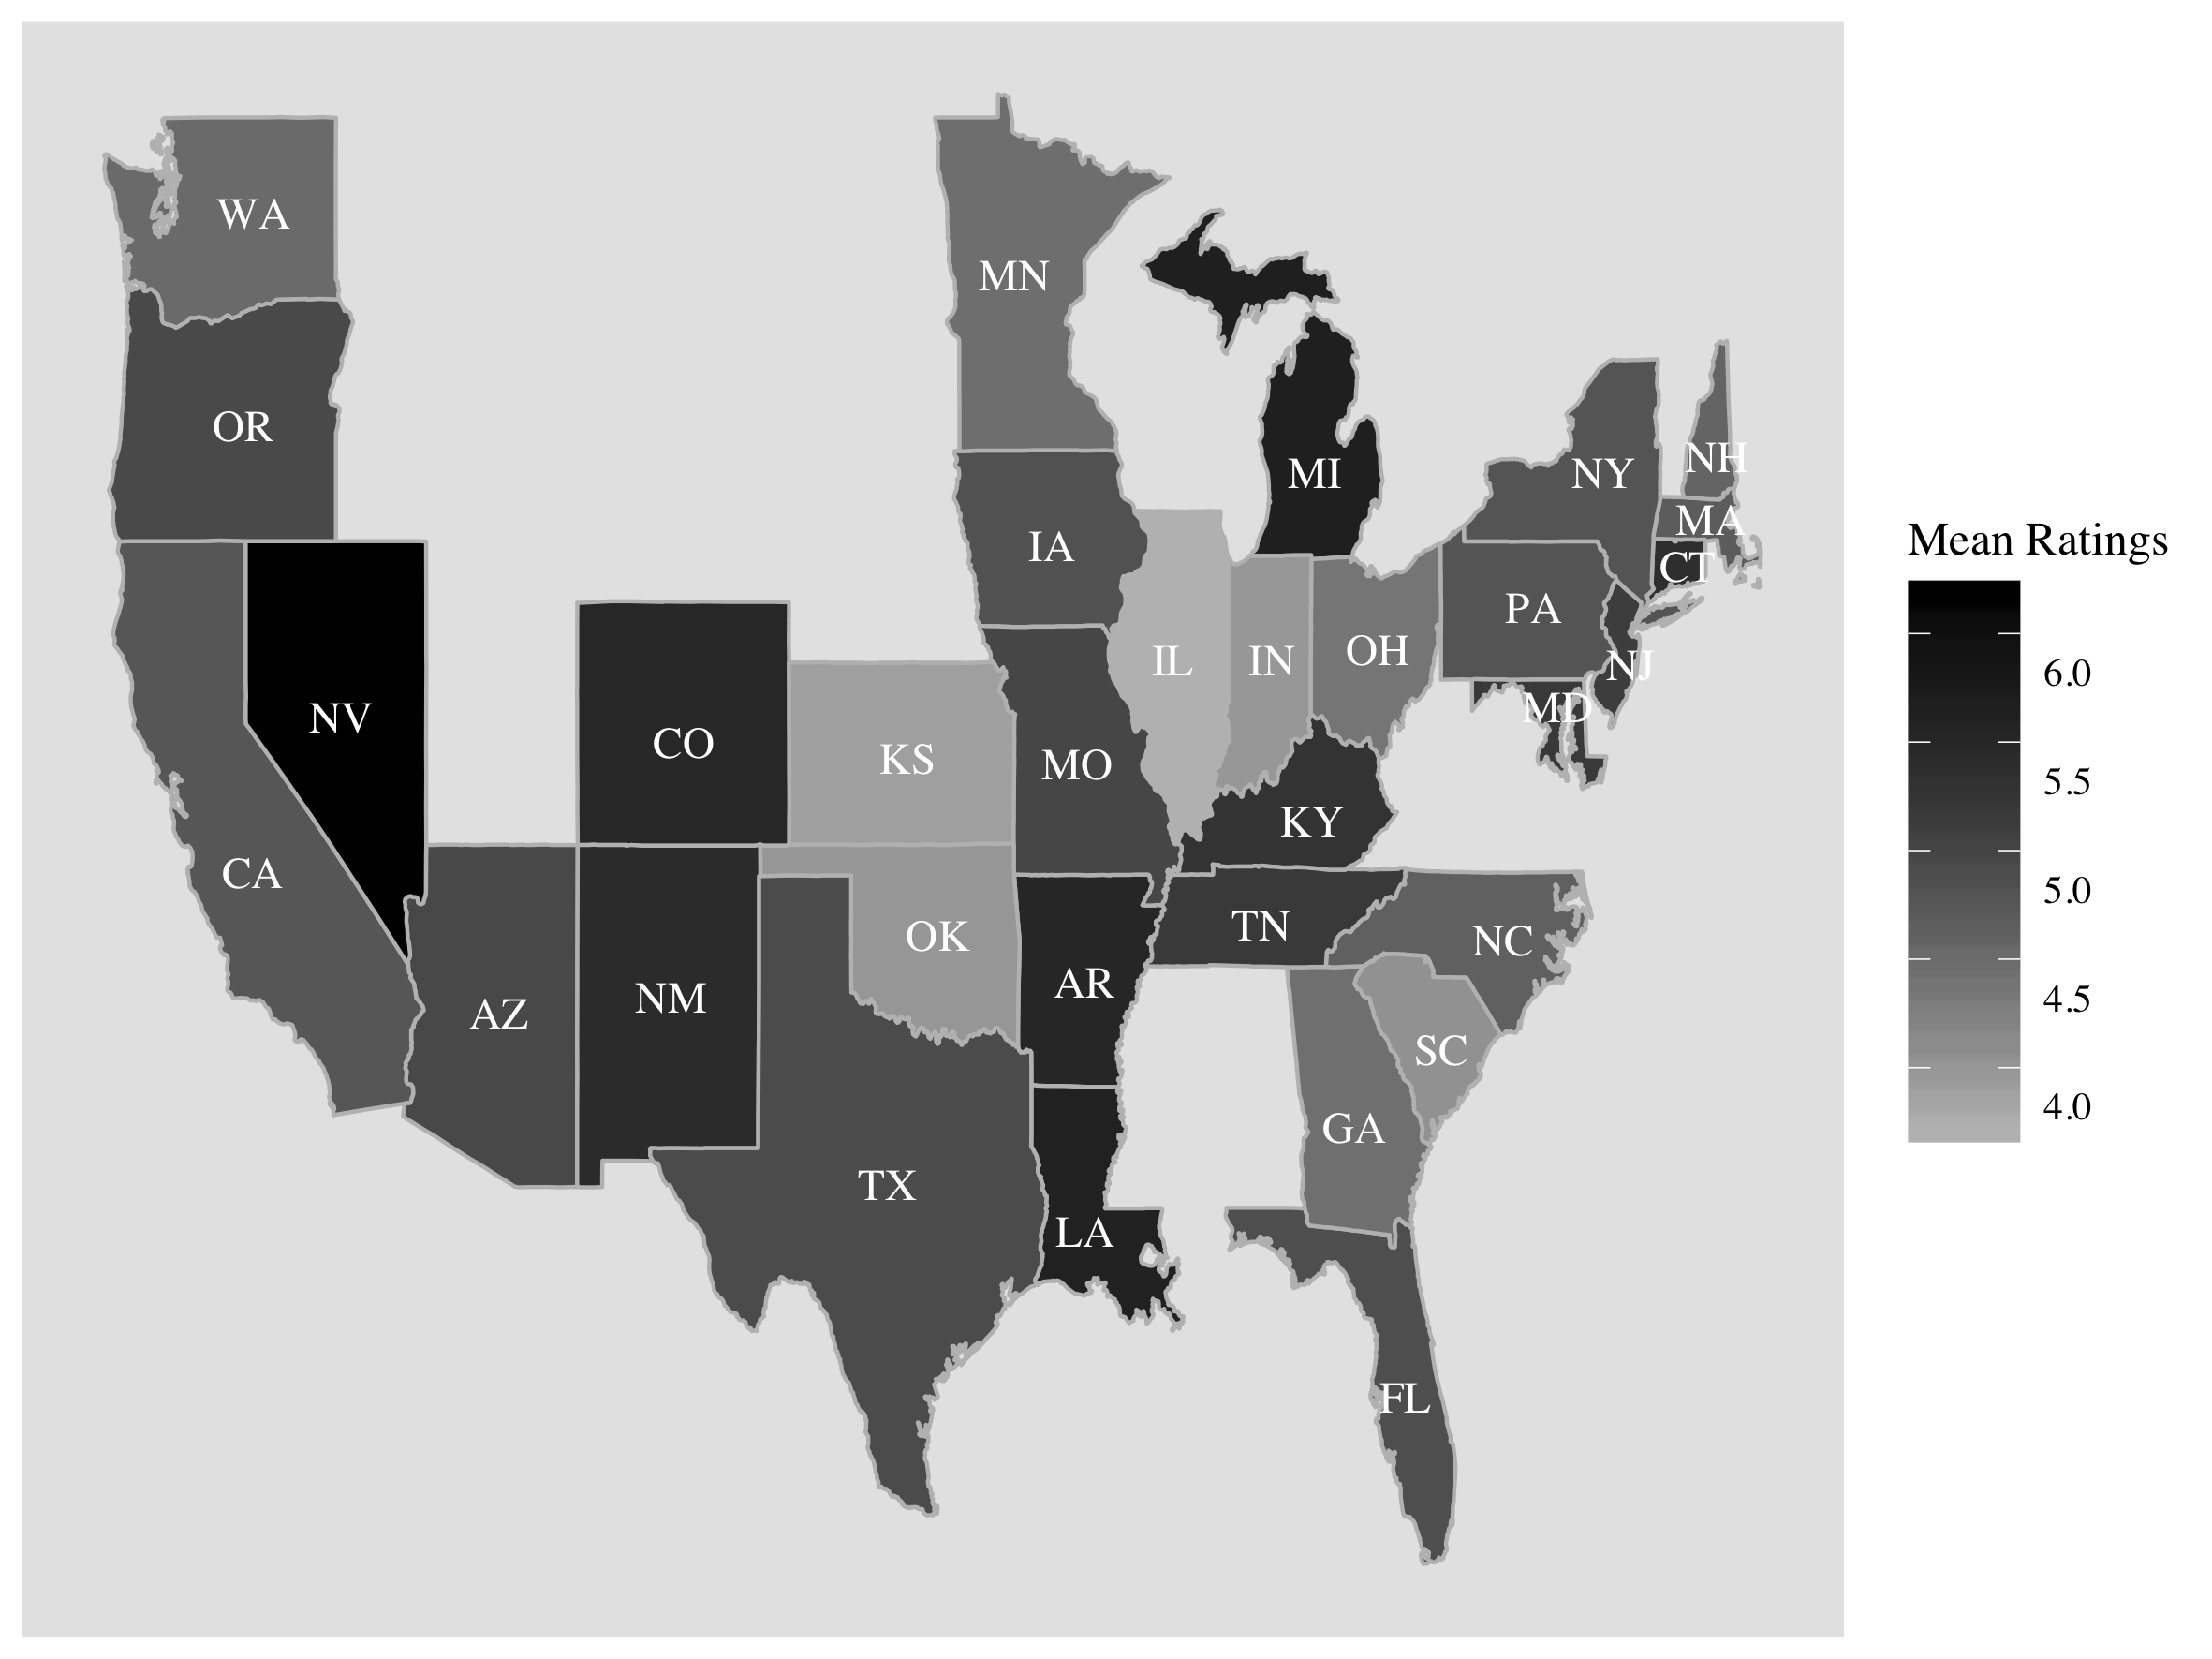
\includegraphics[width=0.8\textwidth]{figures/appendix/exp1.png}
    \caption{Mean Ratings by Birthplace (Experiment 1)}
    \label{fig:bp1}
  \figSpace
\end{figure}

  \figSpace
\begin{figure}[h]
    \centering
    % Created by tikzDevice version 0.12.3 on 2019-12-01 21:36:15
% !TEX encoding = UTF-8 Unicode
\begin{tikzpicture}[x=1pt,y=1pt]
\definecolor{fillColor}{RGB}{255,255,255}
\path[use as bounding box,fill=fillColor,fill opacity=0.00] (0,0) rectangle (397.48,252.94);
\begin{scope}
\path[clip] (  0.00,  0.00) rectangle (397.48,252.94);
\definecolor{drawColor}{RGB}{255,255,255}

\path[draw=drawColor,line width= 0.6pt,line join=round,line cap=round] (  0.00,  0.00) rectangle (397.48,252.94);
\end{scope}
\begin{scope}
\path[clip] (  5.50,  5.50) rectangle (302.87,247.44);

\path[] (  5.50,  5.50) rectangle (302.87,247.44);
\definecolor{drawColor}{RGB}{255,255,255}
\definecolor{fillColor}{RGB}{104,104,104}

\path[draw=drawColor,line width= 0.6pt,line join=round,line cap=round,fill=fillColor] (202.84, 64.20) --
	(202.73, 64.04) --
	(202.53, 64.04) --
	(202.51, 63.68) --
	(202.31, 63.63) --
	(202.22, 63.63) --
	(202.19, 63.47) --
	(202.19, 63.26) --
	(201.80, 63.16) --
	(201.12, 63.00) --
	(200.78, 62.90) --
	(200.58, 62.90) --
	(200.41, 62.90) --
	(200.16, 62.85) --
	(200.10, 62.95) --
	(200.13, 63.11) --
	(200.21, 63.16) --
	(200.41, 63.16) --
	(200.67, 63.21) --
	(201.03, 63.26) --
	(201.18, 63.26) --
	(201.18, 63.63) --
	(201.09, 63.78) --
	(200.98, 64.15) --
	(200.92, 64.30) --
	(200.81, 64.41) --
	(200.67, 64.51) --
	(200.55, 64.72) --
	(200.52, 65.13) --
	(200.47, 65.44) --
	(200.58, 65.76) --
	(200.61, 65.96) --
	(200.55, 66.28) --
	(200.58, 66.74) --
	(200.44, 67.00) --
	(200.24, 67.83) --
	(200.16, 67.89) --
	(200.10, 67.94) --
	(200.01, 67.83) --
	(199.96, 67.52) --
	(199.93, 67.26) --
	(199.93, 67.11) --
	(199.87, 66.90) --
	(199.85, 66.85) --
	(199.79, 66.38) --
	(199.79, 66.22) --
	(199.70, 66.17) --
	(199.65, 66.07) --
	(199.62, 65.96) --
	(199.65, 65.70) --
	(199.59, 65.03) --
	(199.59, 64.67) --
	(199.56, 64.20) --
	(199.53, 63.94) --
	(199.48, 63.78) --
	(199.39, 63.73) --
	(199.34, 63.73) --
	(199.25, 63.89) --
	(199.08, 64.09) --
	(199.02, 64.25) --
	(198.77, 64.30) --
	(198.63, 64.30) --
	(198.54, 64.30) --
	(198.46, 64.51) --
	(198.26, 64.41) --
	(198.18, 67.32) --
	(198.12, 69.71) --
	(198.06, 70.85) --
	(197.95, 73.65) --
	(197.89, 76.04) --
	(197.84, 77.81) --
	(198.06, 80.82) --
	(198.06, 81.60) --
	(198.26, 84.05) --
	(198.46, 87.16) --
	(198.52, 87.74) --
	(198.71, 90.44) --
	(198.83, 92.67) --
	(198.94, 94.54) --
	(199.17, 97.50) --
	(199.17, 97.66) --
	(199.28, 99.79) --
	(199.36,101.14) --
	(199.45,102.23) --
	(199.65,105.09) --
	(199.53,105.14) --
	(199.36,105.56) --
	(199.25,105.97) --
	(199.28,106.13) --
	(200.24,106.13) --
	(202.14,106.08) --
	(204.00,106.03) --
	(204.12,106.03) --
	(205.99,105.97) --
	(206.21,105.92) --
	(208.53,105.92) --
	(210.80,105.87) --
	(211.99,105.82) --
	(212.10,104.57) --
	(212.32,102.54) --
	(212.41,102.23) --
	(212.69, 99.32) --
	(212.89, 97.66) --
	(213.00, 96.57) --
	(213.06, 96.10) --
	(213.29, 93.87) --
	(213.46, 92.36) --
	(213.54, 91.79) --
	(213.80, 88.93) --
	(213.82, 88.83) --
	(214.05, 86.70) --
	(214.05, 86.59) --
	(214.16, 86.44) --
	(214.28, 85.97) --
	(214.36, 85.76) --
	(214.36, 85.61) --
	(214.39, 85.45) --
	(214.50, 84.93) --
	(214.50, 84.57) --
	(214.67, 84.31) --
	(214.76, 83.84) --
	(214.96, 83.58) --
	(215.07, 83.32) --
	(215.04, 83.06) --
	(215.13, 82.64) --
	(215.10, 82.23) --
	(214.98, 81.86) --
	(215.13, 81.60) --
	(215.38, 81.34) --
	(215.49, 81.08) --
	(215.35, 80.93) --
	(215.24, 80.88) --
	(215.15, 80.62) --
	(215.04, 80.46) --
	(214.76, 80.25) --
	(214.70, 79.89) --
	(214.70, 79.73) --
	(214.70, 79.58) --
	(214.70, 79.37) --
	(214.70, 79.06) --
	(214.70, 78.75) --
	(214.62, 78.43) --
	(214.48, 78.23) --
	(214.31, 77.60) --
	(214.33, 76.88) --
	(214.33, 76.77) --
	(214.36, 76.36) --
	(214.42, 75.94) --
	(214.62, 75.32) --
	(214.70, 74.80) --
	(214.70, 74.49) --
	(214.59, 74.07) --
	(214.59, 73.76) --
	(214.53, 73.45) --
	(214.53, 72.82) --
	(214.50, 72.46) --
	(214.39, 72.30) --
	(214.39, 72.04) --
	(214.45, 71.47) --
	(214.45, 71.32) --
	(214.56, 71.00) --
	(214.79, 70.74) --
	(214.82, 70.59) --
	(214.84, 70.43) --
	(214.84, 70.07) --
	(214.93, 69.76) --
	(214.93, 69.71) --
	(212.55, 69.81) --
	(212.44, 69.81) --
	(209.83, 69.81) --
	(209.07, 69.81) --
	(208.14, 69.81) --
	(206.58, 69.81) --
	(206.13, 69.81) --
	(204.23, 69.81) --
	(202.14, 69.81) --
	(202.14, 69.34) --
	(202.11, 69.13) --
	(202.00, 68.82) --
	(201.97, 68.61) --
	(202.00, 68.46) --
	(202.11, 68.30) --
	(202.42, 67.68) --
	(202.70, 67.21) --
	(202.84, 67.11) --
	(202.90, 67.00) --
	(203.04, 66.80) --
	(203.10, 66.54) --
	(203.10, 66.28) --
	(202.99, 65.96) --
	(202.84, 65.60) --
	(202.82, 65.44) --
	(202.84, 65.29) --
	(202.93, 65.13) --
	(203.16, 64.82) --
	(203.18, 64.72) --
	(203.13, 64.56) --
	(203.04, 64.56) --
	(202.96, 64.51) --
	(202.96, 64.46) --
	(202.90, 64.30) --
	(202.84, 64.20) --
	cycle;
\definecolor{fillColor}{RGB}{95,95,95}

\path[draw=drawColor,line width= 0.6pt,line join=round,line cap=round,fill=fillColor] ( 68.62,106.18) --
	( 68.60,106.96) --
	( 68.79,107.12) --
	( 68.94,107.64) --
	( 68.88,108.16) --
	( 68.82,108.57) --
	( 68.77,109.25) --
	( 68.68,109.72) --
	( 68.48,110.13) --
	( 68.51,110.55) --
	( 68.48,110.91) --
	( 68.45,111.53) --
	( 68.40,112.05) --
	( 68.31,112.47) --
	( 68.31,113.20) --
	( 68.37,114.03) --
	( 68.26,114.29) --
	( 68.14,114.70) --
	( 68.14,115.22) --
	( 68.03,115.64) --
	( 68.14,116.05) --
	( 68.31,116.16) --
	( 68.60,116.37) --
	( 69.02,116.47) --
	( 69.36,116.31) --
	( 69.81,116.31) --
	( 70.15,116.11) --
	( 70.24,115.48) --
	( 70.46,115.33) --
	( 70.78,115.27) --
	( 71.09,115.43) --
	( 71.20,115.95) --
	( 71.37,116.31) --
	( 71.51,116.99) --
	( 71.54,122.71) --
	( 71.57,124.11) --
	( 72.64,124.11) --
	( 74.06,124.16) --
	( 75.33,124.16) --
	( 76.69,124.16) --
	( 77.17,124.11) --
	( 78.05,124.16) --
	( 78.98,124.11) --
	( 79.60,124.11) --
	( 80.62,124.11) --
	( 81.90,124.16) --
	( 83.20,124.16) --
	( 84.56,124.16) --
	( 85.01,124.16) --
	( 85.35,124.11) --
	( 85.97,124.11) --
	( 87.36,124.16) --
	( 87.78,124.11) --
	( 88.15,124.11) --
	( 88.83,124.11) --
	( 90.02,124.16) --
	( 91.09,124.16) --
	( 91.49,124.16) --
	( 91.86,124.11) --
	( 92.93,124.11) --
	( 94.43,124.11) --
	( 95.73,124.11) --
	( 96.27,124.11) --
	( 96.24,115.07) --
	( 96.22,105.56) --
	( 96.22,102.13) --
	( 96.19, 94.91) --
	( 96.22, 89.71) --
	( 96.19, 85.87) --
	( 96.19, 82.64) --
	( 96.19, 72.93) --
	( 95.31, 72.93) --
	( 93.39, 72.87) --
	( 91.55, 72.93) --
	( 89.79, 72.93) --
	( 89.17, 72.93) --
	( 88.41, 72.93) --
	( 86.65, 72.87) --
	( 86.00, 72.98) --
	( 85.12, 73.50) --
	( 84.67, 73.76) --
	( 83.48, 74.43) --
	( 81.47, 75.63) --
	( 80.03, 76.46) --
	( 78.36, 77.34) --
	( 77.06, 78.12) --
	( 75.78, 78.85) --
	( 74.99, 79.32) --
	( 74.40, 79.68) --
	( 73.04, 80.51) --
	( 71.60, 81.29) --
	( 70.21, 82.07) --
	( 68.31, 83.16) --
	( 67.78, 83.47) --
	( 67.83, 84.05) --
	( 67.97, 84.88) --
	( 68.14, 85.45) --
	( 68.37, 85.55) --
	( 68.54, 85.50) --
	( 68.85, 85.50) --
	( 69.05, 85.71) --
	( 69.19, 86.28) --
	( 69.42, 86.75) --
	( 69.42, 87.27) --
	( 69.39, 87.84) --
	( 69.11, 88.26) --
	( 68.51, 88.36) --
	( 68.31, 88.62) --
	( 68.26, 89.09) --
	( 68.37, 90.28) --
	( 68.11, 90.70) --
	( 68.23, 91.11) --
	( 68.17, 91.53) --
	( 68.37, 91.79) --
	( 68.57, 92.00) --
	( 68.62, 92.26) --
	( 68.77, 92.41) --
	( 68.71, 92.67) --
	( 68.96, 92.83) --
	( 69.02, 93.09) --
	( 69.16, 93.61) --
	( 69.11, 94.18) --
	( 69.19, 94.49) --
	( 69.11, 94.96) --
	( 69.11, 96.26) --
	( 69.22, 96.62) --
	( 69.53, 96.93) --
	( 69.44, 97.09) --
	( 69.56, 97.30) --
	( 69.70, 97.66) --
	( 69.81, 97.97) --
	( 70.29, 98.34) --
	( 70.63, 98.75) --
	( 70.83, 99.17) --
	( 71.11, 99.32) --
	( 71.09, 99.63) --
	( 70.94,100.00) --
	( 70.35,100.78) --
	( 69.93,101.19) --
	( 69.78,102.28) --
	( 69.70,102.49) --
	( 69.56,103.38) --
	( 68.94,104.26) --
	( 69.05,104.52) --
	( 69.08,104.62) --
	( 68.96,104.78) --
	( 68.77,104.99) --
	( 68.65,105.66) --
	( 68.62,106.18) --
	cycle;
\definecolor{fillColor}{RGB}{78,78,78}

\path[draw=drawColor,line width= 0.6pt,line join=round,line cap=round,fill=fillColor] (170.30, 88.20) --
	(170.30, 90.59) --
	(170.27, 93.09) --
	(170.16, 93.19) --
	(170.10, 93.30) --
	(169.96, 93.24) --
	(169.82, 93.19) --
	(169.79, 93.19) --
	(169.62, 93.40) --
	(169.54, 93.45) --
	(169.45, 93.40) --
	(169.42, 93.30) --
	(169.37, 93.09) --
	(169.25, 93.19) --
	(169.17, 93.19) --
	(169.08, 93.09) --
	(169.03, 93.04) --
	(168.74, 93.09) --
	(168.58, 93.04) --
	(168.55, 93.09) --
	(168.46, 93.30) --
	(168.32, 93.30) --
	(168.26, 93.45) --
	(168.21, 93.61) --
	(168.18, 93.82) --
	(168.09, 93.92) --
	(168.12, 94.02) --
	(168.12, 96.62) --
	(168.15, 98.86) --
	(168.18,101.77) --
	(168.24,103.74) --
	(168.29,105.87) --
	(168.38,109.61) --
	(168.35,110.03) --
	(168.18,111.95) --
	(168.07,112.94) --
	(167.78,116.11) --
	(167.73,116.68) --
	(167.47,119.69) --
	(170.13,119.64) --
	(170.16,119.59) --
	(171.09,119.64) --
	(171.18,119.59) --
	(172.54,119.64) --
	(172.57,119.59) --
	(173.84,119.64) --
	(173.90,119.59) --
	(173.98,119.64) --
	(174.01,119.59) --
	(176.24,119.64) --
	(176.27,119.64) --
	(176.61,119.64) --
	(176.64,119.64) --
	(177.72,119.64) --
	(179.64,119.59) --
	(179.78,119.59) --
	(182.05,119.64) --
	(183.06,119.59) --
	(183.09,119.59) --
	(183.29,119.59) --
	(183.32,119.64) --
	(184.65,119.64) --
	(186.40,119.64) --
	(187.48,119.69) --
	(189.20,119.69) --
	(189.46,119.64) --
	(189.63,119.38) --
	(189.69,118.76) --
	(189.80,118.70) --
	(189.97,118.60) --
	(189.97,118.24) --
	(189.86,117.67) --
	(189.71,117.56) --
	(189.63,117.04) --
	(189.37,116.89) --
	(189.37,116.68) --
	(189.01,116.26) --
	(188.44,115.12) --
	(188.41,115.12) --
	(188.84,115.07) --
	(190.45,115.07) --
	(190.48,115.12) --
	(191.33,115.12) --
	(191.53,115.12) --
	(191.70,115.12) --
	(191.72,114.96) --
	(191.86,114.81) --
	(192.01,114.60) --
	(192.03,114.39) --
	(191.98,114.29) --
	(191.75,114.24) --
	(191.61,114.18) --
	(191.61,113.98) --
	(191.64,113.77) --
	(191.64,113.56) --
	(191.58,113.46) --
	(191.38,113.30) --
	(191.30,113.20) --
	(191.30,113.04) --
	(191.16,112.94) --
	(190.76,112.78) --
	(190.62,112.68) --
	(190.59,112.42) --
	(190.62,112.26) --
	(190.73,112.05) --
	(190.93,112.05) --
	(190.99,111.95) --
	(190.96,111.85) --
	(190.82,111.43) --
	(190.79,111.22) --
	(190.76,111.01) --
	(190.76,110.86) --
	(190.73,110.75) --
	(190.51,110.70) --
	(190.39,110.70) --
	(190.34,110.49) --
	(190.25,109.97) --
	(190.17,109.82) --
	(190.08,109.72) --
	(189.97,109.77) --
	(189.91,109.87) --
	(189.88,110.29) --
	(189.83,110.34) --
	(189.71,110.29) --
	(189.69,110.08) --
	(189.63,109.97) --
	(189.52,109.87) --
	(189.40,109.77) --
	(189.37,109.61) --
	(189.37,109.51) --
	(189.49,109.35) --
	(189.57,109.35) --
	(189.77,109.61) --
	(189.80,109.35) --
	(189.86,109.30) --
	(189.83,109.14) --
	(189.83,108.78) --
	(189.88,108.31) --
	(189.97,108.00) --
	(190.03,107.79) --
	(189.97,107.64) --
	(189.94,107.48) --
	(190.00,107.27) --
	(189.88,107.01) --
	(189.80,106.81) --
	(189.71,106.75) --
	(189.57,106.75) --
	(189.43,106.81) --
	(189.35,106.75) --
	(189.29,106.55) --
	(189.23,106.39) --
	(189.04,106.34) --
	(188.98,106.34) --
	(188.89,106.23) --
	(188.92,105.97) --
	(189.01,105.66) --
	(189.06,105.51) --
	(189.09,105.40) --
	(189.04,105.30) --
	(188.89,105.04) --
	(188.75,104.88) --
	(188.58,104.73) --
	(188.27,104.57) --
	(188.21,104.47) --
	(188.19,104.31) --
	(188.19,104.10) --
	(188.10,103.95) --
	(188.04,103.79) --
	(187.96,103.79) --
	(187.73,103.84) --
	(187.68,103.84) --
	(187.62,103.58) --
	(187.68,103.58) --
	(187.93,103.43) --
	(187.99,103.27) --
	(188.02,103.06) --
	(188.02,102.91) --
	(187.93,102.91) --
	(187.87,103.01) --
	(187.68,103.17) --
	(187.56,103.06) --
	(187.48,102.75) --
	(187.51,102.54) --
	(187.68,102.23) --
	(187.68,102.02) --
	(187.65,101.97) --
	(187.54,101.71) --
	(187.48,101.61) --
	(187.51,100.99) --
	(187.45,100.78) --
	(187.31,100.57) --
	(187.08,100.47) --
	(186.97,100.41) --
	(186.77,100.47) --
	(186.66,100.41) --
	(186.60,100.21) --
	(186.63, 99.95) --
	(186.74, 99.74) --
	(186.66, 99.63) --
	(186.52, 99.63) --
	(186.37, 99.58) --
	(186.26, 99.32) --
	(186.18, 99.17) --
	(186.06, 99.12) --
	(185.87, 99.17) --
	(185.81, 99.06) --
	(185.81, 98.86) --
	(185.89, 98.80) --
	(186.21, 98.70) --
	(186.26, 98.60) --
	(186.21, 98.34) --
	(186.04, 98.34) --
	(185.75, 98.49) --
	(185.55, 98.49) --
	(185.47, 98.34) --
	(185.64, 98.08) --
	(185.72, 97.92) --
	(185.72, 97.61) --
	(185.64, 97.30) --
	(185.55, 97.14) --
	(185.47, 96.93) --
	(185.44, 96.78) --
	(185.33, 96.78) --
	(185.16, 97.09) --
	(185.07, 97.09) --
	(185.02, 97.04) --
	(185.02, 96.78) --
	(185.10, 96.57) --
	(185.13, 96.26) --
	(185.07, 96.10) --
	(185.04, 95.89) --
	(185.10, 95.48) --
	(185.04, 95.22) --
	(184.90, 95.06) --
	(184.71, 94.85) --
	(184.68, 94.59) --
	(184.71, 94.54) --
	(184.99, 94.44) --
	(185.04, 94.18) --
	(184.99, 94.13) --
	(184.82, 94.07) --
	(184.68, 94.13) --
	(184.45, 94.44) --
	(184.37, 94.49) --
	(184.28, 94.33) --
	(184.34, 94.13) --
	(184.37, 93.97) --
	(184.51, 93.66) --
	(184.56, 93.50) --
	(184.54, 93.35) --
	(184.31, 93.24) --
	(184.20, 93.09) --
	(184.22, 92.83) --
	(184.31, 92.67) --
	(184.34, 92.57) --
	(184.25, 92.36) --
	(184.22, 92.15) --
	(184.25, 92.00) --
	(184.34, 92.00) --
	(184.45, 92.20) --
	(184.54, 92.36) --
	(184.65, 92.41) --
	(184.71, 92.31) --
	(184.71, 92.15) --
	(184.56, 92.00) --
	(184.45, 91.74) --
	(184.45, 91.53) --
	(184.48, 91.42) --
	(184.56, 91.42) --
	(184.68, 91.53) --
	(184.82, 91.84) --
	(184.90, 91.89) --
	(184.99, 91.89) --
	(185.02, 91.74) --
	(184.90, 91.48) --
	(184.73, 91.27) --
	(184.56, 91.11) --
	(184.54, 90.96) --
	(184.59, 90.80) --
	(184.76, 90.18) --
	(184.82, 90.13) --
	(184.88, 90.18) --
	(184.93, 90.39) --
	(185.02, 90.44) --
	(185.10, 90.49) --
	(185.13, 90.39) --
	(185.16, 90.18) --
	(185.07, 89.97) --
	(185.02, 89.81) --
	(184.99, 89.61) --
	(184.93, 89.40) --
	(184.73, 89.19) --
	(184.54, 89.19) --
	(184.48, 89.09) --
	(184.45, 88.93) --
	(184.68, 88.57) --
	(184.71, 88.41) --
	(184.65, 88.26) --
	(184.45, 87.89) --
	(184.42, 87.84) --
	(183.94, 87.89) --
	(183.18, 87.89) --
	(183.06, 87.89) --
	(180.12, 87.89) --
	(180.01, 87.89) --
	(176.84, 88.00) --
	(175.54, 88.05) --
	(174.32, 88.05) --
	(173.07, 88.05) --
	(172.90, 88.05) --
	(171.38, 88.10) --
	(170.30, 88.20) --
	cycle;
\definecolor{fillColor}{RGB}{113,113,113}

\path[draw=drawColor,line width= 0.6pt,line join=round,line cap=round,fill=fillColor] ( 42.11,169.57) --
	( 42.11,162.25) --
	( 42.11,148.63) --
	( 42.17,146.30) --
	( 42.11,145.15) --
	( 42.11,143.75) --
	( 42.11,143.33) --
	( 42.11,142.87) --
	( 42.17,142.19) --
	( 42.79,141.46) --
	( 44.26,139.54) --
	( 45.45,138.03) --
	( 46.38,136.84) --
	( 49.95,132.16) --
	( 52.78,128.47) --
	( 56.06,124.00) --
	( 62.40,115.12) --
	( 63.50,113.56) --
	( 68.62,106.18) --
	( 68.65,105.66) --
	( 68.77,104.99) --
	( 68.96,104.78) --
	( 69.08,104.62) --
	( 69.05,104.52) --
	( 68.94,104.26) --
	( 69.56,103.38) --
	( 69.70,102.49) --
	( 69.78,102.28) --
	( 69.93,101.19) --
	( 70.35,100.78) --
	( 70.94,100.00) --
	( 71.09, 99.63) --
	( 71.11, 99.32) --
	( 70.83, 99.17) --
	( 70.63, 98.75) --
	( 70.29, 98.34) --
	( 69.81, 97.97) --
	( 69.70, 97.66) --
	( 69.56, 97.30) --
	( 69.44, 97.09) --
	( 69.53, 96.93) --
	( 69.22, 96.62) --
	( 69.11, 96.26) --
	( 69.11, 94.96) --
	( 69.19, 94.49) --
	( 69.11, 94.18) --
	( 69.16, 93.61) --
	( 69.02, 93.09) --
	( 68.96, 92.83) --
	( 68.71, 92.67) --
	( 68.77, 92.41) --
	( 68.62, 92.26) --
	( 68.57, 92.00) --
	( 68.37, 91.79) --
	( 68.17, 91.53) --
	( 68.23, 91.11) --
	( 68.11, 90.70) --
	( 68.37, 90.28) --
	( 68.26, 89.09) --
	( 68.31, 88.62) --
	( 68.51, 88.36) --
	( 69.11, 88.26) --
	( 69.39, 87.84) --
	( 69.42, 87.27) --
	( 69.42, 86.75) --
	( 69.19, 86.28) --
	( 69.05, 85.71) --
	( 68.85, 85.50) --
	( 68.54, 85.50) --
	( 68.37, 85.55) --
	( 68.14, 85.45) --
	( 61.38, 84.46) --
	( 56.40, 83.68) --
	( 56.40, 84.20) --
	( 56.40, 84.41) --
	( 56.34, 84.62) --
	( 56.17, 84.83) --
	( 56.14, 84.98) --
	( 56.20, 85.03) --
	( 56.46, 84.62) --
	( 56.54, 84.51) --
	( 56.54, 84.72) --
	( 56.48, 85.03) --
	( 56.34, 85.19) --
	( 56.23, 85.35) --
	( 56.17, 85.45) --
	( 56.06, 85.45) --
	( 55.97, 85.19) --
	( 55.92, 85.14) --
	( 55.83, 85.24) --
	( 55.81, 85.61) --
	( 55.92, 85.76) --
	( 55.95, 85.92) --
	( 55.92, 86.02) --
	( 55.83, 86.12) --
	( 55.72, 86.28) --
	( 55.69, 86.54) --
	( 55.81, 86.75) --
	( 55.83, 87.11) --
	( 55.75, 87.79) --
	( 55.72, 88.15) --
	( 55.55, 88.83) --
	( 55.38, 89.24) --
	( 55.21, 89.81) --
	( 54.96, 90.28) --
	( 54.81, 90.70) --
	( 54.62, 90.96) --
	( 54.36, 91.27) --
	( 54.16, 91.53) --
	( 54.08, 91.79) --
	( 53.77, 92.05) --
	( 53.60, 92.26) --
	( 53.43, 92.46) --
	( 53.29, 92.78) --
	( 53.06, 93.19) --
	( 52.83, 93.50) --
	( 52.66, 93.61) --
	( 52.55, 93.61) --
	( 52.35, 93.87) --
	( 51.98, 94.44) --
	( 51.73, 94.70) --
	( 51.62, 94.80) --
	( 51.56, 94.91) --
	( 51.33, 95.01) --
	( 51.16, 95.06) --
	( 50.99, 94.91) --
	( 50.85, 94.91) --
	( 50.85, 94.70) --
	( 50.80, 94.54) --
	( 50.63, 94.54) --
	( 50.51, 94.65) --
	( 50.40, 94.70) --
	( 50.20, 94.80) --
	( 50.09, 94.96) --
	( 50.09, 95.17) --
	( 50.17, 95.37) --
	( 50.20, 95.63) --
	( 50.09, 96.15) --
	( 49.83, 96.78) --
	( 49.78, 97.04) --
	( 49.64, 97.19) --
	( 49.38, 97.30) --
	( 48.76, 97.40) --
	( 48.42, 97.30) --
	( 48.19, 97.24) --
	( 48.02, 97.30) --
	( 47.43, 97.56) --
	( 47.34, 97.66) --
	( 47.12, 97.76) --
	( 46.95, 98.02) --
	( 46.81, 98.02) --
	( 46.58, 97.97) --
	( 46.30, 98.34) --
	( 46.10, 99.01) --
	( 45.96, 99.37) --
	( 45.90, 99.58) --
	( 45.45, 99.84) --
	( 45.14,100.26) --
	( 44.91,100.62) --
	( 44.66,100.73) --
	( 44.43,100.88) --
	( 44.20,100.93) --
	( 43.78,100.73) --
	( 43.50,100.83) --
	( 43.24,100.88) --
	( 42.93,100.83) --
	( 42.70,100.93) --
	( 42.39,101.14) --
	( 42.17,101.19) --
	( 41.83,101.19) --
	( 41.51,101.25) --
	( 40.78,101.19) --
	( 40.16,101.14) --
	( 40.01,101.25) --
	( 39.84,101.61) --
	( 39.67,101.97) --
	( 39.34,102.13) --
	( 39.14,102.23) --
	( 39.08,102.65) --
	( 39.25,103.17) --
	( 39.25,103.69) --
	( 39.11,104.05) --
	( 39.14,104.42) --
	( 39.31,104.78) --
	( 39.17,105.09) --
	( 39.11,105.25) --
	( 39.02,105.45) --
	( 39.08,105.66) --
	( 39.08,106.13) --
	( 39.17,106.49) --
	( 39.19,107.17) --
	( 39.08,107.53) --
	( 38.91,107.69) --
	( 38.74,107.74) --
	( 38.71,107.58) --
	( 38.60,107.58) --
	( 38.37,107.90) --
	( 38.12,108.10) --
	( 37.92,108.57) --
	( 37.92,108.83) --
	( 38.06,109.14) --
	( 38.12,109.14) --
	( 38.20,109.04) --
	( 38.26,109.09) --
	( 38.12,109.66) --
	( 37.98,110.03) --
	( 37.95,110.23) --
	( 37.75,110.23) --
	( 37.35,110.29) --
	( 37.18,110.60) --
	( 36.84,111.22) --
	( 36.59,111.74) --
	( 36.39,111.90) --
	( 36.14,112.21) --
	( 35.97,112.42) --
	( 35.85,112.78) --
	( 35.85,113.14) --
	( 35.68,113.25) --
	( 35.54,113.56) --
	( 35.35,113.82) --
	( 35.18,114.03) --
	( 35.01,114.34) --
	( 34.89,114.91) --
	( 34.75,115.27) --
	( 34.55,115.48) --
	( 34.38,115.95) --
	( 34.13,116.57) --
	( 33.90,116.83) --
	( 33.76,117.09) --
	( 33.59,117.15) --
	( 33.34,117.35) --
	( 33.11,117.72) --
	( 32.94,117.98) --
	( 32.94,118.24) --
	( 32.94,118.55) --
	( 32.80,119.28) --
	( 32.77,119.59) --
	( 32.60,119.85) --
	( 32.60,119.95) --
	( 32.71,120.00) --
	( 32.66,120.32) --
	( 32.60,120.37) --
	( 32.69,120.73) --
	( 32.80,120.89) --
	( 33.00,120.83) --
	( 33.08,120.78) --
	( 33.28,121.04) --
	( 33.39,121.61) --
	( 33.45,122.13) --
	( 33.42,122.71) --
	( 33.39,122.81) --
	( 33.42,123.07) --
	( 33.25,123.33) --
	( 33.08,123.69) --
	( 32.83,123.90) --
	( 32.71,124.00) --
	( 32.63,123.85) --
	( 32.49,123.85) --
	( 32.40,123.95) --
	( 32.20,123.85) --
	( 32.09,123.85) --
	( 31.75,124.00) --
	( 31.47,124.32) --
	( 31.21,124.63) --
	( 31.10,124.99) --
	( 30.99,125.15) --
	( 30.82,125.25) --
	( 30.76,125.46) --
	( 30.68,125.56) --
	( 30.59,125.87) --
	( 30.42,126.13) --
	( 30.34,126.50) --
	( 30.36,126.97) --
	( 30.42,127.38) --
	( 30.39,127.85) --
	( 30.28,127.95) --
	( 30.19,128.21) --
	( 30.19,128.58) --
	( 30.14,128.73) --
	( 29.94,128.84) --
	( 29.86,129.15) --
	( 29.86,129.36) --
	( 29.86,129.72) --
	( 30.00,129.88) --
	( 30.00,130.03) --
	( 29.94,130.24) --
	( 30.00,130.50) --
	( 29.94,130.66) --
	( 29.88,131.07) --
	( 29.88,131.28) --
	( 30.00,131.33) --
	( 30.05,131.33) --
	( 30.22,131.54) --
	( 30.28,131.43) --
	( 30.36,131.43) --
	( 30.56,131.43) --
	( 30.56,131.28) --
	( 30.59,131.07) --
	( 30.68,130.81) --
	( 30.56,130.76) --
	( 30.48,130.66) --
	( 30.48,130.50) --
	( 30.53,130.29) --
	( 30.62,130.14) --
	( 30.59,129.93) --
	( 30.56,129.72) --
	( 30.73,129.62) --
	( 31.02,129.51) --
	( 31.19,129.36) --
	( 31.30,129.15) --
	( 31.50,128.99) --
	( 31.69,128.89) --
	( 31.81,128.73) --
	( 31.86,128.68) --
	( 31.95,128.52) --
	( 32.03,128.42) --
	( 32.23,128.32) --
	( 32.40,128.32) --
	( 32.52,128.47) --
	( 32.49,128.47) --
	( 32.49,128.63) --
	( 32.26,128.73) --
	( 32.03,128.94) --
	( 31.89,129.10) --
	( 31.81,129.51) --
	( 31.69,130.03) --
	( 31.55,130.50) --
	( 31.33,130.81) --
	( 31.07,131.07) --
	( 30.90,131.33) --
	( 30.93,131.69) --
	( 30.90,131.85) --
	( 30.90,132.06) --
	( 30.90,132.32) --
	( 30.76,132.47) --
	( 30.62,132.58) --
	( 30.48,132.63) --
	( 30.39,132.89) --
	( 30.45,132.94) --
	( 30.53,133.15) --
	( 30.59,133.36) --
	( 30.59,133.46) --
	( 30.82,133.46) --
	( 30.96,133.46) --
	( 31.04,133.67) --
	( 31.19,133.77) --
	( 31.10,133.77) --
	( 31.50,133.72) --
	( 31.64,133.67) --
	( 31.58,133.82) --
	( 31.38,133.93) --
	( 31.19,134.08) --
	( 31.02,134.24) --
	( 31.02,134.50) --
	( 30.85,134.60) --
	( 30.73,134.50) --
	( 30.53,134.66) --
	( 30.42,134.81) --
	( 30.31,134.86) --
	( 30.19,134.71) --
	( 30.17,134.50) --
	( 30.08,134.45) --
	( 29.94,134.50) --
	( 29.80,134.50) --
	( 29.88,134.34) --
	( 29.97,134.34) --
	( 29.94,133.93) --
	( 29.88,133.72) --
	( 29.88,133.46) --
	( 29.94,133.41) --
	( 30.08,133.31) --
	( 30.14,133.25) --
	( 30.14,133.10) --
	( 30.00,133.05) --
	( 29.97,132.89) --
	( 30.00,132.73) --
	( 30.05,132.58) --
	( 30.17,132.42) --
	( 30.25,132.32) --
	( 30.25,132.16) --
	( 30.19,132.11) --
	( 30.08,132.27) --
	( 30.00,132.32) --
	( 29.94,132.27) --
	( 30.00,132.06) --
	( 30.02,131.85) --
	( 30.00,131.75) --
	( 29.86,131.80) --
	( 29.77,131.85) --
	( 29.63,132.01) --
	( 29.54,132.16) --
	( 29.32,132.27) --
	( 29.20,132.47) --
	( 29.12,132.58) --
	( 29.06,132.58) --
	( 29.01,132.47) --
	( 28.95,132.58) --
	( 28.72,132.79) --
	( 28.53,132.94) --
	( 28.41,133.20) --
	( 28.16,133.46) --
	( 27.93,133.57) --
	( 27.90,133.67) --
	( 27.87,133.88) --
	( 27.70,133.72) --
	( 27.65,133.41) --
	( 27.59,133.31) --
	( 27.48,133.25) --
	( 27.39,133.41) --
	( 27.42,133.72) --
	( 27.56,134.24) --
	( 27.62,134.50) --
	( 27.59,134.92) --
	( 27.51,135.23) --
	( 27.62,135.28) --
	( 27.73,135.02) --
	( 27.87,134.92) --
	( 27.93,135.02) --
	( 27.87,135.38) --
	( 27.68,135.70) --
	( 27.59,135.96) --
	( 27.48,136.06) --
	( 27.34,136.22) --
	( 27.17,136.22) --
	( 27.05,136.68) --
	( 26.88,137.25) --
	( 26.63,137.72) --
	( 26.29,137.93) --
	( 25.98,138.14) --
	( 25.72,138.61) --
	( 25.55,139.18) --
	( 25.30,139.70) --
	( 25.07,139.85) --
	( 24.96,140.06) --
	( 24.87,140.27) --
	( 24.68,140.53) --
	( 24.51,140.74) --
	( 24.42,141.05) --
	( 24.14,141.26) --
	( 23.91,141.67) --
	( 23.77,141.93) --
	( 23.83,142.24) --
	( 23.94,142.66) --
	( 24.00,142.97) --
	( 23.71,143.75) --
	( 23.43,144.79) --
	( 23.35,145.41) --
	( 23.32,146.24) --
	( 23.43,146.82) --
	( 23.57,147.39) --
	( 23.54,147.91) --
	( 23.57,148.32) --
	( 23.49,148.63) --
	( 23.35,149.10) --
	( 23.35,149.62) --
	( 23.09,150.09) --
	( 22.87,150.19) --
	( 22.81,150.61) --
	( 22.64,150.92) --
	( 22.50,151.13) --
	( 22.38,151.44) --
	( 22.24,151.65) --
	( 22.16,151.80) --
	( 22.02,152.17) --
	( 21.99,152.48) --
	( 21.76,152.69) --
	( 21.62,152.84) --
	( 21.39,153.15) --
	( 21.14,153.52) --
	( 20.88,153.73) --
	( 20.66,154.04) --
	( 20.63,154.25) --
	( 20.74,154.71) --
	( 20.69,155.13) --
	( 20.49,155.44) --
	( 20.52,156.06) --
	( 20.74,157.00) --
	( 20.97,157.73) --
	( 21.34,158.71) --
	( 21.62,159.60) --
	( 21.82,160.27) --
	( 21.93,160.79) --
	( 21.76,161.31) --
	( 21.62,161.83) --
	( 21.68,162.09) --
	( 21.73,162.35) --
	( 21.93,162.14) --
	( 21.99,162.35) --
	( 21.93,162.97) --
	( 22.10,163.55) --
	( 22.16,164.12) --
	( 22.19,164.53) --
	( 22.19,164.64) --
	( 22.10,165.05) --
	( 22.04,165.21) --
	( 22.02,165.42) --
	( 22.19,165.42) --
	( 22.10,165.73) --
	( 21.90,166.09) --
	( 21.85,166.61) --
	( 21.73,166.98) --
	( 21.62,167.34) --
	( 21.45,167.50) --
	( 21.28,167.76) --
	( 21.22,168.12) --
	( 21.28,168.53) --
	( 21.39,168.95) --
	( 21.45,169.26) --
	( 21.48,169.52) --
	( 23.15,169.57) --
	( 24.62,169.57) --
	( 26.15,169.57) --
	( 30.76,169.57) --
	( 34.86,169.57) --
	( 37.75,169.68) --
	( 42.11,169.57) --
	cycle;
\definecolor{fillColor}{gray}{0.70}

\path[draw=drawColor,line width= 0.6pt,line join=round,line cap=round,fill=fillColor] (130.77,151.44) --
	(130.74,151.39) --
	(130.77,147.54) --
	(130.77,147.44) --
	(130.77,143.49) --
	(130.77,142.76) --
	(130.80,139.49) --
	(130.80,138.76) --
	(130.80,135.54) --
	(130.82,130.81) --
	(130.82,130.03) --
	(130.80,127.64) --
	(130.80,124.16) --
	(130.43,124.00) --
	(129.66,124.00) --
	(128.65,124.00) --
	(127.34,124.00) --
	(126.66,124.00) --
	(126.07,124.16) --
	(125.67,124.11) --
	(125.28,124.00) --
	(124.17,124.00) --
	(122.96,124.00) --
	(121.77,124.00) --
	(121.09,124.00) --
	(120.61,124.00) --
	(119.19,124.00) --
	(117.21,124.00) --
	(115.71,124.00) --
	(115.03,124.00) --
	(114.30,124.00) --
	(113.25,124.00) --
	(112.66,124.00) --
	(111.24,124.00) --
	(108.95,124.00) --
	(108.33,124.00) --
	(106.80,124.00) --
	(104.99,124.11) --
	(104.17,124.00) --
	(104.08,124.11) --
	(103.63,124.11) --
	(101.82,124.11) --
	(100.06,124.11) --
	( 99.47,124.11) --
	( 98.99,124.16) --
	( 98.00,124.11) --
	( 96.87,124.11) --
	( 96.27,124.11) --
	( 96.22,129.88) --
	( 96.24,132.01) --
	( 96.22,134.60) --
	( 96.19,137.83) --
	( 96.19,145.57) --
	( 96.16,146.82) --
	( 96.19,148.22) --
	( 96.19,153.36) --
	( 96.19,157.31) --
	( 96.22,160.38) --
	( 96.19,160.32) --
	(101.79,160.58) --
	(104.82,160.58) --
	(107.05,160.53) --
	(109.66,160.48) --
	(110.28,160.48) --
	(110.25,160.53) --
	(114.81,160.48) --
	(116.51,160.53) --
	(120.86,160.48) --
	(123.27,160.48) --
	(124.26,160.48) --
	(127.80,160.48) --
	(127.99,160.48) --
	(130.74,160.43) --
	(130.74,158.14) --
	(130.71,157.73) --
	(130.74,157.62) --
	(130.71,155.34) --
	(130.71,154.51) --
	(130.77,151.44) --
	cycle;
\definecolor{fillColor}{RGB}{85,85,85}

\path[draw=drawColor,line width= 0.6pt,line join=round,line cap=round,fill=fillColor] (271.81,169.94) --
	(274.07,169.89) --
	(274.21,169.89) --
	(275.18,169.83) --
	(275.18,169.57) --
	(275.46,169.52) --
	(275.52,169.83) --
	(276.48,169.78) --
	(276.73,169.83) --
	(278.57,169.83) --
	(278.71,169.78) --
	(280.18,169.83) --
	(280.27,169.57) --
	(280.30,166.98) --
	(280.30,166.25) --
	(280.30,165.88) --
	(280.30,164.59) --
	(280.27,164.33) --
	(280.16,164.33) --
	(280.02,164.22) --
	(279.99,164.07) --
	(279.96,163.96) --
	(279.99,163.55) --
	(279.31,163.44) --
	(279.19,163.29) --
	(278.97,163.23) --
	(278.80,163.29) --
	(278.69,163.29) --
	(278.60,163.18) --
	(278.49,163.18) --
	(278.37,163.29) --
	(278.23,163.29) --
	(278.18,163.13) --
	(278.03,163.13) --
	(277.84,162.97) --
	(277.72,162.92) --
	(277.61,162.97) --
	(277.44,163.39) --
	(277.33,163.23) --
	(277.33,163.13) --
	(277.36,162.97) --
	(277.30,162.87) --
	(277.21,162.77) --
	(276.99,162.92) --
	(276.85,162.87) --
	(276.59,162.77) --
	(276.34,162.77) --
	(276.11,162.87) --
	(276.00,162.87) --
	(275.86,162.87) --
	(275.74,162.77) --
	(275.60,162.77) --
	(275.35,162.77) --
	(275.15,162.77) --
	(274.92,162.72) --
	(274.78,162.66) --
	(274.69,163.13) --
	(274.53,163.13) --
	(274.41,162.77) --
	(274.33,162.51) --
	(274.16,162.25) --
	(273.93,162.20) --
	(273.79,162.09) --
	(273.73,161.99) --
	(273.70,161.83) --
	(273.65,161.73) --
	(273.53,161.73) --
	(273.36,161.88) --
	(273.22,161.88) --
	(273.08,161.73) --
	(272.97,161.52) --
	(272.88,161.47) --
	(272.49,161.52) --
	(272.35,161.52) --
	(272.29,161.47) --
	(272.18,161.21) --
	(272.06,161.05) --
	(271.89,160.84) --
	(271.75,160.84) --
	(271.72,160.69) --
	(271.50,160.58) --
	(271.16,160.53) --
	(270.96,160.64) --
	(270.70,161.42) --
	(271.61,162.20) --
	(271.81,162.40) --
	(271.50,163.18) --
	(271.53,163.75) --
	(271.58,165.26) --
	(271.64,166.56) --
	(271.81,169.94) --
	cycle;
\definecolor{fillColor}{gray}{0.40}

\path[draw=drawColor,line width= 0.6pt,line join=round,line cap=round,fill=fillColor] (214.93, 69.71) --
	(215.01, 69.39) --
	(215.13, 69.03) --
	(215.27, 68.82) --
	(215.30, 68.72) --
	(215.27, 68.46) --
	(215.30, 67.78) --
	(215.47, 67.42) --
	(215.61, 67.26) --
	(215.66, 67.16) --
	(218.10, 66.90) --
	(218.41, 66.90) --
	(219.51, 66.80) --
	(219.88, 66.74) --
	(221.13, 66.64) --
	(221.95, 66.54) --
	(222.99, 66.38) --
	(223.47, 66.38) --
	(224.27, 66.28) --
	(226.33, 66.02) --
	(226.84, 65.96) --
	(227.55, 65.86) --
	(228.77, 65.76) --
	(228.71, 65.55) --
	(228.62, 65.44) --
	(228.68, 65.29) --
	(228.77, 65.13) --
	(228.79, 64.92) --
	(228.79, 64.25) --
	(228.94, 64.04) --
	(229.02, 63.94) --
	(229.22, 63.94) --
	(229.39, 63.89) --
	(229.59, 63.94) --
	(229.59, 64.15) --
	(229.64, 64.67) --
	(229.67, 65.34) --
	(229.70, 65.70) --
	(229.67, 65.96) --
	(229.59, 66.28) --
	(229.56, 67.06) --
	(229.56, 67.32) --
	(229.59, 67.47) --
	(229.70, 67.63) --
	(229.70, 67.83) --
	(229.76, 67.89) --
	(229.90, 67.83) --
	(229.95, 67.89) --
	(230.01, 67.99) --
	(230.10, 68.15) --
	(230.18, 68.15) --
	(230.35, 68.20) --
	(230.44, 67.99) --
	(230.63, 67.83) --
	(230.80, 67.83) --
	(230.95, 67.63) --
	(231.06, 67.68) --
	(231.14, 67.57) --
	(231.34, 67.32) --
	(231.45, 67.42) --
	(231.54, 67.42) --
	(231.62, 67.26) --
	(231.79, 67.21) --
	(232.02, 67.16) --
	(232.11, 66.90) --
	(232.16, 66.90) --
	(232.25, 66.80) --
	(232.28, 66.74) --
	(232.39, 66.80) --
	(232.47, 66.85) --
	(232.53, 66.85) --
	(232.53, 66.74) --
	(232.47, 66.48) --
	(232.45, 66.28) --
	(232.42, 66.07) --
	(232.50, 65.81) --
	(232.50, 65.70) --
	(232.53, 65.50) --
	(232.53, 65.34) --
	(232.59, 65.08) --
	(232.61, 64.82) --
	(232.59, 64.41) --
	(232.50, 64.20) --
	(232.53, 64.04) --
	(232.59, 63.99) --
	(232.67, 64.04) --
	(232.78, 64.20) --
	(232.84, 64.15) --
	(232.93, 63.57) --
	(232.95, 62.90) --
	(233.01, 62.38) --
	(233.12, 61.55) --
	(233.32, 60.35) --
	(233.38, 59.94) --
	(233.32, 59.57) --
	(233.44, 59.42) --
	(233.52, 59.16) --
	(233.52, 58.74) --
	(233.55, 58.17) --
	(233.61, 57.96) --
	(233.72, 57.86) --
	(233.78, 57.70) --
	(233.78, 57.44) --
	(233.97, 56.61) --
	(234.23, 55.52) --
	(234.34, 55.05) --
	(234.34, 54.84) --
	(234.79, 53.44) --
	(234.91, 53.08) --
	(234.96, 52.66) --
	(234.96, 52.14) --
	(235.02, 52.09) --
	(235.11, 52.09) --
	(235.22, 51.99) --
	(235.25, 51.73) --
	(235.25, 51.31) --
	(235.47, 50.64) --
	(235.81, 49.86) --
	(235.95, 49.44) --
	(235.93, 49.28) --
	(235.84, 49.28) --
	(235.61, 49.65) --
	(235.53, 49.65) --
	(235.50, 49.54) --
	(235.67, 48.45) --
	(235.84, 47.36) --
	(236.15, 45.60) --
	(236.52, 44.04) --
	(236.77, 43.15) --
	(237.11, 41.85) --
	(237.34, 41.18) --
	(237.51, 40.66) --
	(237.65, 39.98) --
	(237.82, 39.36) --
	(237.94, 39.00) --
	(238.05, 38.42) --
	(238.08, 38.06) --
	(238.08, 37.70) --
	(238.16, 37.39) --
	(238.36, 36.66) --
	(238.50, 36.14) --
	(238.64, 35.77) --
	(238.73, 35.26) --
	(238.67, 35.00) --
	(238.67, 34.84) --
	(238.81, 34.74) --
	(238.95, 34.68) --
	(239.04, 34.53) --
	(239.12, 34.16) --
	(239.24, 33.59) --
	(239.29, 33.07) --
	(239.35, 32.66) --
	(239.43, 31.93) --
	(239.46, 31.31) --
	(239.49, 30.58) --
	(239.46, 29.90) --
	(239.41, 29.07) --
	(239.32, 28.03) --
	(239.27, 27.25) --
	(239.27, 26.94) --
	(239.21, 25.90) --
	(239.15, 25.49) --
	(239.10, 25.23) --
	(239.07, 24.86) --
	(239.07, 24.45) --
	(239.04, 24.03) --
	(239.01, 23.51) --
	(239.07, 23.04) --
	(239.07, 22.73) --
	(239.07, 22.52) --
	(239.04, 22.42) --
	(238.98, 22.37) --
	(238.90, 22.42) --
	(238.87, 22.58) --
	(238.87, 22.78) --
	(238.90, 23.10) --
	(238.84, 23.10) --
	(238.78, 23.04) --
	(238.73, 22.89) --
	(238.70, 22.47) --
	(238.67, 22.16) --
	(238.61, 22.01) --
	(238.44, 21.85) --
	(238.39, 21.64) --
	(238.33, 21.12) --
	(238.22, 21.02) --
	(238.16, 20.91) --
	(238.10, 20.76) --
	(238.10, 20.45) --
	(238.10, 20.29) --
	(238.05, 20.08) --
	(237.96, 19.82) --
	(237.94, 19.51) --
	(237.99, 19.15) --
	(238.08, 18.89) --
	(238.08, 18.68) --
	(238.05, 18.52) --
	(237.79, 18.32) --
	(237.77, 18.06) --
	(237.71, 17.95) --
	(237.60, 17.80) --
	(237.54, 17.48) --
	(237.51, 17.33) --
	(237.37, 17.43) --
	(237.28, 17.38) --
	(237.23, 17.17) --
	(237.14, 17.17) --
	(236.94, 17.43) --
	(236.80, 17.48) --
	(236.75, 17.43) --
	(236.77, 17.17) --
	(236.69, 17.07) --
	(236.58, 17.07) --
	(236.35, 16.97) --
	(236.18, 16.76) --
	(235.78, 16.76) --
	(235.61, 16.91) --
	(235.50, 16.97) --
	(235.27, 16.97) --
	(235.02, 16.65) --
	(234.94, 16.60) --
	(234.79, 16.55) --
	(234.54, 16.60) --
	(234.34, 16.50) --
	(234.23, 16.55) --
	(234.11, 16.76) --
	(233.94, 17.17) --
	(233.89, 17.48) --
	(233.86, 17.74) --
	(233.89, 18.06) --
	(233.94, 18.21) --
	(234.06, 18.26) --
	(234.17, 18.21) --
	(234.26, 18.06) --
	(234.37, 17.80) --
	(234.51, 17.54) --
	(234.65, 17.43) --
	(234.79, 17.33) --
	(234.96, 17.43) --
	(235.08, 17.54) --
	(235.13, 17.64) --
	(235.11, 17.85) --
	(235.13, 18.00) --
	(235.16, 18.16) --
	(235.16, 18.26) --
	(235.11, 18.32) --
	(234.94, 18.26) --
	(234.85, 18.26) --
	(234.82, 18.32) --
	(234.77, 18.52) --
	(234.68, 18.58) --
	(234.65, 18.58) --
	(234.45, 18.78) --
	(234.40, 18.78) --
	(234.26, 18.73) --
	(234.20, 18.78) --
	(234.00, 18.94) --
	(233.92, 19.15) --
	(233.89, 19.62) --
	(233.80, 19.77) --
	(233.69, 19.98) --
	(233.66, 20.08) --
	(233.72, 20.29) --
	(233.69, 20.39) --
	(233.55, 20.50) --
	(233.52, 20.65) --
	(233.35, 21.28) --
	(233.21, 21.54) --
	(233.12, 21.69) --
	(232.98, 22.27) --
	(232.87, 22.58) --
	(232.73, 22.84) --
	(232.47, 23.15) --
	(232.28, 23.30) --
	(232.16, 23.36) --
	(232.08, 23.56) --
	(231.96, 23.56) --
	(231.91, 23.46) --
	(231.74, 23.62) --
	(231.62, 23.56) --
	(231.54, 23.62) --
	(231.43, 23.67) --
	(231.34, 23.62) --
	(231.26, 23.62) --
	(231.20, 23.67) --
	(231.06, 23.82) --
	(230.89, 24.40) --
	(230.69, 25.59) --
	(230.58, 26.53) --
	(230.55, 27.05) --
	(230.55, 27.36) --
	(230.55, 27.77) --
	(230.55, 27.98) --
	(230.44, 28.14) --
	(230.44, 28.29) --
	(230.44, 28.50) --
	(230.38, 28.50) --
	(230.24, 28.40) --
	(230.15, 28.45) --
	(229.98, 28.81) --
	(229.87, 28.81) --
	(229.79, 29.02) --
	(229.79, 29.12) --
	(229.90, 29.28) --
	(229.87, 29.38) --
	(229.73, 29.38) --
	(229.59, 29.38) --
	(229.53, 29.49) --
	(229.50, 29.70) --
	(229.50, 30.06) --
	(229.45, 30.27) --
	(229.36, 30.42) --
	(229.33, 30.63) --
	(229.36, 31.05) --
	(229.42, 31.31) --
	(229.50, 31.62) --
	(229.45, 32.19) --
	(229.36, 32.45) --
	(229.28, 32.66) --
	(229.30, 32.76) --
	(229.36, 32.87) --
	(229.59, 32.97) --
	(229.64, 33.07) --
	(229.64, 33.23) --
	(229.59, 33.28) --
	(229.45, 33.18) --
	(229.33, 33.12) --
	(229.25, 33.12) --
	(229.19, 33.12) --
	(229.08, 33.12) --
	(228.99, 33.07) --
	(228.65, 33.44) --
	(228.57, 33.49) --
	(228.54, 33.44) --
	(228.54, 33.23) --
	(228.62, 33.07) --
	(228.96, 32.40) --
	(229.02, 32.14) --
	(229.02, 31.83) --
	(228.96, 31.77) --
	(228.82, 31.83) --
	(228.77, 31.88) --
	(228.65, 31.88) --
	(228.60, 31.83) --
	(228.51, 32.03) --
	(228.43, 31.98) --
	(228.37, 32.14) --
	(228.17, 32.50) --
	(228.12, 32.92) --
	(228.03, 33.02) --
	(227.92, 33.18) --
	(227.80, 33.44) --
	(227.72, 33.75) --
	(227.52, 34.16) --
	(227.46, 34.37) --
	(227.46, 34.53) --
	(227.49, 34.84) --
	(227.44, 35.10) --
	(227.27, 35.52) --
	(227.12, 36.19) --
	(227.04, 36.61) --
	(227.04, 36.97) --
	(227.01, 37.18) --
	(226.84, 37.39) --
	(226.73, 37.54) --
	(226.50, 37.65) --
	(226.47, 37.75) --
	(226.53, 38.11) --
	(226.56, 38.27) --
	(226.59, 38.27) --
	(226.70, 38.27) --
	(226.93, 38.22) --
	(226.96, 38.32) --
	(226.93, 38.68) --
	(226.90, 38.74) --
	(226.87, 38.84) --
	(226.90, 38.94) --
	(227.01, 39.10) --
	(227.04, 39.31) --
	(227.04, 39.41) --
	(227.07, 39.52) --
	(227.15, 39.57) --
	(227.27, 39.67) --
	(227.35, 39.83) --
	(227.46, 39.93) --
	(227.49, 40.04) --
	(227.46, 40.24) --
	(227.46, 40.35) --
	(227.52, 40.45) --
	(227.69, 40.56) --
	(227.92, 41.13) --
	(227.89, 41.28) --
	(227.86, 41.39) --
	(227.80, 41.49) --
	(227.78, 41.75) --
	(227.80, 42.01) --
	(227.69, 42.06) --
	(227.66, 42.17) --
	(227.61, 42.17) --
	(227.55, 42.11) --
	(227.52, 41.91) --
	(227.44, 41.70) --
	(227.46, 41.33) --
	(227.44, 41.18) --
	(227.38, 41.07) --
	(227.29, 41.13) --
	(227.24, 41.18) --
	(227.15, 41.39) --
	(227.15, 41.59) --
	(227.15, 41.91) --
	(227.15, 42.17) --
	(227.04, 42.32) --
	(226.84, 42.43) --
	(226.76, 42.58) --
	(226.67, 42.69) --
	(226.59, 42.63) --
	(226.56, 42.63) --
	(226.47, 42.74) --
	(226.45, 42.89) --
	(226.39, 42.95) --
	(226.36, 42.89) --
	(226.33, 42.53) --
	(226.33, 42.32) --
	(226.28, 42.22) --
	(226.22, 42.17) --
	(226.22, 41.96) --
	(226.28, 41.91) --
	(226.50, 41.80) --
	(226.59, 41.54) --
	(226.70, 41.49) --
	(226.73, 41.39) --
	(226.67, 41.28) --
	(226.67, 41.23) --
	(226.70, 41.02) --
	(226.70, 40.76) --
	(226.67, 40.61) --
	(226.67, 40.50) --
	(226.67, 40.24) --
	(226.64, 40.04) --
	(226.56, 39.98) --
	(226.45, 39.98) --
	(226.39, 40.09) --
	(226.36, 40.19) --
	(226.28, 40.24) --
	(226.19, 40.30) --
	(226.11, 40.40) --
	(226.08, 40.50) --
	(226.02, 41.02) --
	(225.99, 41.13) --
	(225.94, 41.18) --
	(225.85, 41.18) --
	(225.82, 41.02) --
	(225.77, 41.02) --
	(225.74, 41.07) --
	(225.65, 41.33) --
	(225.63, 41.65) --
	(225.63, 41.85) --
	(225.71, 42.17) --
	(225.85, 42.63) --
	(225.94, 43.00) --
	(225.94, 43.36) --
	(225.94, 43.67) --
	(225.88, 44.09) --
	(225.88, 44.24) --
	(225.99, 44.45) --
	(226.16, 44.97) --
	(226.19, 45.02) --
	(226.22, 45.28) --
	(226.22, 45.65) --
	(226.28, 45.91) --
	(226.33, 46.12) --
	(226.36, 46.32) --
	(226.45, 46.53) --
	(226.47, 46.69) --
	(226.42, 46.84) --
	(226.47, 47.21) --
	(226.53, 47.31) --
	(226.56, 47.52) --
	(226.56, 47.83) --
	(226.50, 48.14) --
	(226.50, 48.35) --
	(226.53, 48.51) --
	(226.59, 48.61) --
	(226.67, 48.87) --
	(226.67, 49.02) --
	(226.59, 49.23) --
	(226.59, 49.39) --
	(226.64, 49.54) --
	(226.64, 49.65) --
	(226.64, 49.80) --
	(226.53, 49.86) --
	(226.45, 49.91) --
	(226.39, 50.01) --
	(226.39, 50.12) --
	(226.39, 50.17) --
	(226.42, 50.32) --
	(226.47, 50.38) --
	(226.59, 50.38) --
	(226.67, 50.38) --
	(226.73, 50.48) --
	(226.76, 50.58) --
	(226.70, 50.69) --
	(226.59, 50.90) --
	(226.39, 51.05) --
	(226.30, 51.21) --
	(226.25, 51.31) --
	(226.25, 51.57) --
	(226.19, 51.67) --
	(226.13, 51.88) --
	(226.16, 52.09) --
	(226.16, 52.19) --
	(226.13, 52.25) --
	(226.08, 52.35) --
	(225.91, 52.40) --
	(225.85, 52.45) --
	(225.82, 52.66) --
	(225.85, 52.87) --
	(225.88, 52.97) --
	(225.82, 53.13) --
	(225.63, 53.18) --
	(225.46, 53.18) --
	(225.00, 53.29) --
	(224.83, 53.29) --
	(224.66, 53.39) --
	(224.55, 53.49) --
	(224.52, 53.65) --
	(224.52, 53.81) --
	(224.55, 53.96) --
	(224.44, 54.22) --
	(224.30, 54.27) --
	(224.18, 54.27) --
	(224.13, 54.38) --
	(224.07, 54.64) --
	(224.07, 54.90) --
	(223.96, 55.21) --
	(223.84, 55.42) --
	(223.73, 55.57) --
	(223.64, 55.62) --
	(223.56, 55.62) --
	(223.50, 55.62) --
	(223.42, 55.57) --
	(223.36, 55.73) --
	(223.33, 55.88) --
	(223.25, 56.09) --
	(223.16, 56.14) --
	(223.05, 56.25) --
	(222.97, 56.35) --
	(222.91, 56.46) --
	(222.94, 56.82) --
	(222.91, 56.97) --
	(222.85, 57.29) --
	(222.85, 57.70) --
	(222.65, 57.81) --
	(222.48, 57.91) --
	(222.46, 58.17) --
	(222.37, 58.22) --
	(222.29, 58.17) --
	(222.17, 58.22) --
	(222.09, 58.53) --
	(221.95, 58.64) --
	(221.92, 58.79) --
	(221.92, 58.95) --
	(222.00, 59.05) --
	(222.03, 59.16) --
	(221.95, 59.31) --
	(221.80, 59.42) --
	(221.64, 59.73) --
	(221.44, 60.09) --
	(221.21, 60.30) --
	(221.04, 60.56) --
	(220.87, 60.56) --
	(220.79, 60.61) --
	(220.22, 61.39) --
	(220.02, 61.60) --
	(219.80, 61.70) --
	(219.57, 61.65) --
	(219.43, 61.60) --
	(219.29, 61.50) --
	(219.17, 61.50) --
	(219.06, 61.55) --
	(218.89, 61.70) --
	(218.81, 61.70) --
	(218.72, 61.70) --
	(218.58, 61.70) --
	(218.58, 61.44) --
	(218.55, 61.34) --
	(218.44, 61.34) --
	(218.27, 61.34) --
	(218.18, 61.29) --
	(218.01, 61.03) --
	(218.01, 60.87) --
	(218.13, 60.61) --
	(218.13, 60.56) --
	(217.96, 60.56) --
	(217.87, 60.56) --
	(217.81, 60.51) --
	(217.93, 60.40) --
	(218.10, 60.30) --
	(218.21, 60.20) --
	(218.24, 60.04) --
	(218.18, 59.94) --
	(218.13, 59.83) --
	(218.10, 59.83) --
	(217.90, 59.88) --
	(217.79, 60.04) --
	(217.70, 60.09) --
	(217.64, 60.09) --
	(217.56, 60.04) --
	(217.48, 59.94) --
	(217.36, 59.99) --
	(217.31, 59.99) --
	(217.16, 59.94) --
	(216.85, 59.57) --
	(216.40, 59.26) --
	(215.95, 58.85) --
	(215.72, 58.64) --
	(215.58, 58.48) --
	(215.52, 58.48) --
	(215.49, 58.53) --
	(215.52, 58.79) --
	(215.58, 58.90) --
	(215.49, 59.00) --
	(215.41, 59.00) --
	(215.27, 58.95) --
	(215.27, 58.74) --
	(215.18, 58.64) --
	(215.07, 58.64) --
	(215.01, 58.53) --
	(214.96, 58.33) --
	(214.90, 58.27) --
	(214.70, 58.27) --
	(214.39, 58.33) --
	(214.16, 58.33) --
	(214.05, 58.33) --
	(213.94, 58.17) --
	(213.82, 58.01) --
	(213.71, 58.01) --
	(213.54, 58.01) --
	(213.43, 58.01) --
	(213.32, 57.91) --
	(213.20, 57.81) --
	(213.12, 57.81) --
	(213.03, 57.86) --
	(212.86, 58.27) --
	(212.81, 58.69) --
	(212.75, 59.00) --
	(212.78, 59.26) --
	(212.78, 59.47) --
	(212.83, 59.57) --
	(212.89, 59.73) --
	(212.98, 59.78) --
	(213.00, 59.78) --
	(213.00, 59.05) --
	(212.98, 58.74) --
	(213.00, 58.38) --
	(213.12, 58.12) --
	(213.20, 58.01) --
	(213.29, 58.17) --
	(213.37, 58.48) --
	(213.40, 58.85) --
	(213.37, 59.26) --
	(213.26, 59.57) --
	(213.15, 59.78) --
	(213.06, 60.09) --
	(213.06, 60.25) --
	(212.98, 60.35) --
	(212.78, 60.40) --
	(212.61, 60.51) --
	(212.49, 60.61) --
	(212.41, 60.72) --
	(212.41, 60.98) --
	(211.62, 61.70) --
	(211.59, 61.86) --
	(211.59, 61.96) --
	(211.67, 61.96) --
	(211.87, 61.86) --
	(212.44, 61.34) --
	(212.52, 61.34) --
	(212.55, 61.44) --
	(212.47, 61.60) --
	(212.41, 62.02) --
	(212.30, 62.07) --
	(212.21, 62.07) --
	(212.07, 61.96) --
	(211.96, 62.02) --
	(211.76, 62.22) --
	(211.65, 62.22) --
	(211.53, 62.33) --
	(211.39, 62.59) --
	(211.53, 62.74) --
	(211.53, 62.95) --
	(211.62, 63.05) --
	(211.62, 63.16) --
	(211.56, 63.16) --
	(211.45, 63.11) --
	(211.39, 63.11) --
	(211.33, 63.21) --
	(211.28, 63.52) --
	(211.16, 63.63) --
	(211.02, 63.63) --
	(210.94, 63.42) --
	(210.82, 63.37) --
	(210.71, 63.16) --
	(210.71, 63.00) --
	(210.80, 62.90) --
	(210.91, 62.90) --
	(211.05, 63.11) --
	(211.14, 63.11) --
	(211.14, 62.95) --
	(211.16, 62.85) --
	(211.28, 62.85) --
	(211.28, 62.74) --
	(211.28, 62.53) --
	(211.31, 62.07) --
	(211.28, 62.02) --
	(211.16, 62.07) --
	(210.68, 62.69) --
	(210.32, 63.05) --
	(210.12, 63.26) --
	(209.89, 63.47) --
	(209.30, 63.78) --
	(208.76, 64.09) --
	(208.39, 64.25) --
	(208.08, 64.30) --
	(207.91, 64.41) --
	(207.71, 64.46) --
	(207.63, 64.46) --
	(207.54, 64.56) --
	(207.54, 64.72) --
	(207.57, 64.72) --
	(207.71, 64.72) --
	(207.94, 64.67) --
	(208.08, 64.72) --
	(208.22, 64.61) --
	(208.33, 64.67) --
	(208.42, 64.77) --
	(208.48, 64.77) --
	(208.56, 64.72) --
	(208.65, 64.72) --
	(208.84, 64.72) --
	(209.04, 64.61) --
	(209.24, 64.51) --
	(209.35, 64.56) --
	(209.38, 64.61) --
	(209.38, 64.77) --
	(209.27, 64.98) --
	(209.10, 65.18) --
	(208.90, 65.34) --
	(208.84, 65.34) --
	(208.79, 65.34) --
	(208.65, 65.24) --
	(208.59, 65.18) --
	(208.42, 65.24) --
	(208.28, 65.29) --
	(208.08, 65.13) --
	(207.97, 65.13) --
	(207.88, 65.13) --
	(207.83, 65.24) --
	(207.77, 65.34) --
	(207.74, 65.50) --
	(207.68, 65.50) --
	(207.57, 65.50) --
	(207.54, 65.34) --
	(207.57, 65.24) --
	(207.54, 65.08) --
	(207.46, 65.03) --
	(207.32, 65.08) --
	(207.26, 65.03) --
	(207.17, 64.82) --
	(207.06, 64.82) --
	(206.98, 64.72) --
	(206.72, 64.72) --
	(206.33, 64.72) --
	(206.10, 64.72) --
	(205.73, 64.61) --
	(205.36, 64.56) --
	(205.00, 64.41) --
	(204.74, 64.30) --
	(204.54, 64.25) --
	(204.43, 64.15) --
	(204.32, 64.15) --
	(204.23, 64.15) --
	(204.20, 64.20) --
	(204.20, 64.25) --
	(204.26, 64.30) --
	(204.34, 64.46) --
	(204.51, 64.51) --
	(204.74, 64.61) --
	(204.85, 64.61) --
	(205.02, 64.72) --
	(205.19, 64.98) --
	(205.25, 65.03) --
	(205.25, 65.18) --
	(205.22, 65.29) --
	(205.11, 65.34) --
	(205.05, 65.50) --
	(205.05, 65.65) --
	(205.05, 65.86) --
	(205.02, 65.96) --
	(204.97, 65.96) --
	(204.88, 65.76) --
	(204.77, 65.34) --
	(204.74, 65.13) --
	(204.68, 65.08) --
	(204.60, 65.08) --
	(204.51, 65.13) --
	(204.51, 65.29) --
	(204.54, 65.55) --
	(204.49, 65.65) --
	(204.40, 65.76) --
	(204.29, 65.96) --
	(204.20, 66.02) --
	(204.12, 66.02) --
	(204.15, 65.81) --
	(204.20, 65.65) --
	(204.26, 65.34) --
	(204.23, 65.08) --
	(204.15, 64.82) --
	(204.03, 64.67) --
	(203.84, 64.51) --
	(203.67, 64.30) --
	(203.61, 64.30) --
	(203.58, 64.15) --
	(203.55, 64.04) --
	(203.47, 64.04) --
	(203.24, 63.99) --
	(203.18, 63.94) --
	(203.13, 63.78) --
	(203.10, 63.73) --
	(202.96, 63.68) --
	(202.70, 63.52) --
	(202.62, 63.52) --
	(202.59, 63.63) --
	(202.59, 63.68) --
	(202.82, 63.89) --
	(202.84, 63.94) --
	(202.84, 64.20) --
	(202.90, 64.30) --
	(202.96, 64.46) --
	(202.96, 64.51) --
	(203.04, 64.56) --
	(203.13, 64.56) --
	(203.18, 64.72) --
	(203.16, 64.82) --
	(202.93, 65.13) --
	(202.84, 65.29) --
	(202.82, 65.44) --
	(202.84, 65.60) --
	(202.99, 65.96) --
	(203.10, 66.28) --
	(203.10, 66.54) --
	(203.04, 66.80) --
	(202.90, 67.00) --
	(202.84, 67.11) --
	(202.70, 67.21) --
	(202.42, 67.68) --
	(202.11, 68.30) --
	(202.00, 68.46) --
	(201.97, 68.61) --
	(202.00, 68.82) --
	(202.11, 69.13) --
	(202.14, 69.34) --
	(202.14, 69.81) --
	(204.23, 69.81) --
	(206.13, 69.81) --
	(206.58, 69.81) --
	(208.14, 69.81) --
	(209.07, 69.81) --
	(209.83, 69.81) --
	(212.44, 69.81) --
	(212.55, 69.81) --
	(214.93, 69.71) --
	cycle;
\definecolor{fillColor}{RGB}{136,136,136}

\path[draw=drawColor,line width= 0.6pt,line join=round,line cap=round,fill=fillColor] (235.30, 79.16) --
	(235.50, 79.06) --
	(235.53, 78.95) --
	(235.50, 78.75) --
	(235.33, 78.54) --
	(235.11, 78.43) --
	(234.99, 78.38) --
	(234.94, 78.28) --
	(234.96, 78.12) --
	(235.02, 77.92) --
	(234.82, 77.71) --
	(234.71, 77.66) --
	(234.57, 77.76) --
	(234.28, 77.81) --
	(234.23, 77.71) --
	(234.20, 77.55) --
	(234.31, 77.50) --
	(234.34, 77.29) --
	(234.40, 77.29) --
	(234.57, 77.24) --
	(234.57, 77.14) --
	(234.54, 77.03) --
	(234.40, 76.88) --
	(234.34, 76.77) --
	(234.23, 76.46) --
	(234.14, 76.36) --
	(234.06, 76.51) --
	(233.89, 76.56) --
	(233.78, 76.36) --
	(233.86, 76.30) --
	(233.86, 75.94) --
	(233.92, 75.84) --
	(234.09, 75.99) --
	(234.11, 75.94) --
	(234.11, 75.68) --
	(234.09, 75.32) --
	(234.00, 75.01) --
	(233.94, 74.80) --
	(233.80, 74.95) --
	(233.75, 75.01) --
	(233.63, 74.90) --
	(233.52, 74.80) --
	(233.41, 74.80) --
	(233.35, 74.64) --
	(233.35, 74.49) --
	(233.41, 74.43) --
	(233.49, 74.43) --
	(233.55, 74.54) --
	(233.72, 74.59) --
	(233.78, 74.59) --
	(233.80, 74.49) --
	(233.80, 74.38) --
	(233.75, 74.17) --
	(233.63, 73.97) --
	(233.55, 73.45) --
	(233.52, 73.34) --
	(233.32, 73.50) --
	(233.27, 73.45) --
	(233.18, 73.39) --
	(233.15, 73.19) --
	(233.15, 72.93) --
	(233.15, 72.77) --
	(233.07, 72.67) --
	(232.76, 72.82) --
	(232.64, 72.82) --
	(232.59, 72.67) --
	(232.56, 72.67) --
	(232.67, 72.51) --
	(232.78, 72.15) --
	(232.78, 72.10) --
	(232.73, 71.99) --
	(232.64, 71.84) --
	(232.59, 71.63) --
	(232.56, 71.58) --
	(232.59, 71.06) --
	(232.59, 70.95) --
	(232.53, 70.90) --
	(232.42, 70.90) --
	(232.25, 71.21) --
	(232.19, 71.37) --
	(232.13, 71.42) --
	(232.08, 71.37) --
	(232.13, 71.21) --
	(232.16, 71.11) --
	(232.11, 70.90) --
	(232.16, 70.80) --
	(232.28, 70.69) --
	(232.36, 70.59) --
	(232.39, 70.28) --
	(232.45, 70.02) --
	(232.59, 70.17) --
	(232.61, 70.33) --
	(232.67, 70.69) --
	(232.73, 70.74) --
	(232.76, 70.69) --
	(232.78, 70.54) --
	(232.78, 70.33) --
	(232.76, 70.07) --
	(232.67, 69.91) --
	(232.59, 69.91) --
	(232.50, 69.81) --
	(232.42, 69.71) --
	(232.30, 69.71) --
	(232.25, 69.65) --
	(232.25, 69.50) --
	(232.30, 69.39) --
	(232.42, 69.45) --
	(232.50, 69.45) --
	(232.56, 69.39) --
	(232.53, 69.24) --
	(232.39, 69.03) --
	(232.30, 68.82) --
	(232.28, 68.67) --
	(232.28, 68.46) --
	(232.22, 68.30) --
	(232.19, 68.15) --
	(232.19, 67.99) --
	(232.36, 67.73) --
	(232.36, 67.57) --
	(232.25, 67.26) --
	(232.02, 67.16) --
	(231.79, 67.21) --
	(231.62, 67.26) --
	(231.54, 67.42) --
	(231.45, 67.42) --
	(231.34, 67.32) --
	(231.14, 67.57) --
	(231.06, 67.68) --
	(230.95, 67.63) --
	(230.80, 67.83) --
	(230.63, 67.83) --
	(230.44, 67.99) --
	(230.35, 68.20) --
	(230.18, 68.15) --
	(230.10, 68.15) --
	(230.01, 67.99) --
	(229.95, 67.89) --
	(229.90, 67.83) --
	(229.76, 67.89) --
	(229.70, 67.83) --
	(229.70, 67.63) --
	(229.59, 67.47) --
	(229.56, 67.32) --
	(229.56, 67.06) --
	(229.59, 66.28) --
	(229.67, 65.96) --
	(229.70, 65.70) --
	(229.67, 65.34) --
	(229.64, 64.67) --
	(229.59, 64.15) --
	(229.59, 63.94) --
	(229.39, 63.89) --
	(229.22, 63.94) --
	(229.02, 63.94) --
	(228.94, 64.04) --
	(228.79, 64.25) --
	(228.79, 64.92) --
	(228.77, 65.13) --
	(228.68, 65.29) --
	(228.62, 65.44) --
	(228.71, 65.55) --
	(228.77, 65.76) --
	(227.55, 65.86) --
	(226.84, 65.96) --
	(226.33, 66.02) --
	(224.27, 66.28) --
	(223.47, 66.38) --
	(222.99, 66.38) --
	(221.95, 66.54) --
	(221.13, 66.64) --
	(219.88, 66.74) --
	(219.51, 66.80) --
	(218.41, 66.90) --
	(218.10, 66.90) --
	(215.66, 67.16) --
	(215.61, 67.26) --
	(215.47, 67.42) --
	(215.30, 67.78) --
	(215.27, 68.46) --
	(215.30, 68.72) --
	(215.27, 68.82) --
	(215.13, 69.03) --
	(215.01, 69.39) --
	(214.93, 69.71) --
	(214.93, 69.76) --
	(214.84, 70.07) --
	(214.84, 70.43) --
	(214.82, 70.59) --
	(214.79, 70.74) --
	(214.56, 71.00) --
	(214.45, 71.32) --
	(214.45, 71.47) --
	(214.39, 72.04) --
	(214.39, 72.30) --
	(214.50, 72.46) --
	(214.53, 72.82) --
	(214.53, 73.45) --
	(214.59, 73.76) --
	(214.59, 74.07) --
	(214.70, 74.49) --
	(214.70, 74.80) --
	(214.62, 75.32) --
	(214.42, 75.94) --
	(214.36, 76.36) --
	(214.33, 76.77) --
	(214.33, 76.88) --
	(214.31, 77.60) --
	(214.48, 78.23) --
	(214.62, 78.43) --
	(214.70, 78.75) --
	(214.70, 79.06) --
	(214.70, 79.37) --
	(214.70, 79.58) --
	(214.70, 79.73) --
	(214.70, 79.89) --
	(214.76, 80.25) --
	(215.04, 80.46) --
	(215.15, 80.62) --
	(215.24, 80.88) --
	(215.35, 80.93) --
	(215.49, 81.08) --
	(215.38, 81.34) --
	(215.13, 81.60) --
	(214.98, 81.86) --
	(215.10, 82.23) --
	(215.13, 82.64) --
	(215.04, 83.06) --
	(215.07, 83.32) --
	(214.96, 83.58) --
	(214.76, 83.84) --
	(214.67, 84.31) --
	(214.50, 84.57) --
	(214.50, 84.93) --
	(214.39, 85.45) --
	(214.36, 85.61) --
	(214.36, 85.76) --
	(214.28, 85.97) --
	(214.16, 86.44) --
	(214.05, 86.59) --
	(214.05, 86.70) --
	(213.82, 88.83) --
	(213.80, 88.93) --
	(213.54, 91.79) --
	(213.46, 92.36) --
	(213.29, 93.87) --
	(213.06, 96.10) --
	(213.00, 96.57) --
	(212.89, 97.66) --
	(212.69, 99.32) --
	(212.41,102.23) --
	(212.32,102.54) --
	(212.10,104.57) --
	(211.99,105.82) --
	(212.75,105.82) --
	(213.20,105.82) --
	(213.65,105.82) --
	(215.04,105.82) --
	(215.86,105.87) --
	(216.12,105.87) --
	(216.82,105.87) --
	(218.32,105.87) --
	(218.35,105.97) --
	(218.35,105.92) --
	(219.23,105.82) --
	(219.85,105.82) --
	(220.19,105.82) --
	(222.00,105.92) --
	(222.34,105.92) --
	(224.21,105.97) --
	(224.35,105.92) --
	(224.24,105.66) --
	(224.18,105.45) --
	(223.98,105.25) --
	(223.36,104.31) --
	(223.28,104.10) --
	(223.13,103.69) --
	(223.08,103.53) --
	(223.08,103.32) --
	(223.16,103.06) --
	(223.33,102.96) --
	(223.53,102.54) --
	(223.67,102.54) --
	(223.87,102.49) --
	(223.98,102.39) --
	(224.10,102.23) --
	(224.35,101.71) --
	(224.58,101.45) --
	(224.86,101.35) --
	(225.09,101.30) --
	(225.37,101.25) --
	(225.51,101.14) --
	(225.60,100.88) --
	(225.68,100.31) --
	(225.77,100.10) --
	(225.94, 99.69) --
	(226.11, 99.27) --
	(226.16, 98.86) --
	(226.19, 98.65) --
	(226.25, 98.44) --
	(226.42, 98.18) --
	(226.53, 98.02) --
	(226.67, 97.66) --
	(226.76, 97.50) --
	(226.84, 97.40) --
	(226.90, 97.14) --
	(227.04, 96.57) --
	(227.10, 96.47) --
	(227.32, 96.15) --
	(227.41, 95.95) --
	(227.52, 95.84) --
	(227.78, 95.69) --
	(228.00, 95.43) --
	(228.31, 95.01) --
	(228.40, 94.91) --
	(228.51, 94.70) --
	(228.60, 94.49) --
	(228.74, 94.13) --
	(228.82, 93.76) --
	(228.96, 93.45) --
	(229.05, 93.30) --
	(229.25, 93.24) --
	(229.36, 93.19) --
	(229.62, 92.83) --
	(229.81, 92.57) --
	(229.90, 92.36) --
	(230.18, 92.05) --
	(230.18, 91.94) --
	(230.15, 91.79) --
	(230.10, 91.53) --
	(230.12, 91.37) --
	(230.10, 91.17) --
	(230.15, 90.96) --
	(230.46, 90.75) --
	(230.58, 90.33) --
	(230.55, 90.13) --
	(230.58, 89.97) --
	(230.75, 89.81) --
	(230.89, 89.87) --
	(231.00, 89.71) --
	(230.95, 89.45) --
	(231.00, 89.29) --
	(231.12, 89.03) --
	(231.40, 88.83) --
	(231.65, 88.67) --
	(232.02, 88.26) --
	(232.25, 88.05) --
	(232.36, 87.84) --
	(232.30, 87.27) --
	(232.42, 87.11) --
	(232.50, 86.85) --
	(232.53, 86.54) --
	(232.67, 86.44) --
	(232.70, 85.87) --
	(232.73, 85.50) --
	(232.67, 85.35) --
	(232.67, 85.19) --
	(232.76, 84.93) --
	(232.76, 84.72) --
	(232.73, 84.57) --
	(232.81, 84.31) --
	(232.98, 84.05) --
	(233.10, 83.99) --
	(233.32, 83.84) --
	(233.78, 83.16) --
	(233.80, 83.01) --
	(233.86, 82.64) --
	(233.97, 82.23) --
	(234.09, 81.92) --
	(234.14, 81.71) --
	(234.11, 81.50) --
	(234.06, 80.88) --
	(233.97, 80.46) --
	(234.00, 80.25) --
	(234.09, 79.99) --
	(234.14, 79.84) --
	(234.31, 79.68) --
	(234.51, 79.63) --
	(234.77, 79.58) --
	(234.94, 79.42) --
	(235.13, 79.27) --
	(235.30, 79.16) --
	cycle;
\definecolor{fillColor}{RGB}{172,172,172}

\path[draw=drawColor,line width= 0.6pt,line join=round,line cap=round,fill=fillColor] ( 56.82,169.57) --
	( 56.82,184.75) --
	( 56.82,185.73) --
	( 57.05,186.57) --
	( 57.19,187.24) --
	( 57.28,187.71) --
	( 57.16,188.12) --
	( 57.16,188.44) --
	( 57.33,188.75) --
	( 57.42,188.96) --
	( 57.36,189.42) --
	( 57.19,189.63) --
	( 56.94,189.94) --
	( 56.71,189.73) --
	( 56.48,190.10) --
	( 56.17,189.99) --
	( 55.95,190.20) --
	( 55.95,190.41) --
	( 55.95,190.67) --
	( 55.86,190.88) --
	( 55.81,191.19) --
	( 55.92,191.61) --
	( 55.95,192.12) --
	( 56.26,192.64) --
	( 56.57,193.79) --
	( 56.77,194.41) --
	( 56.99,194.62) --
	( 57.25,194.72) --
	( 57.36,195.03) --
	( 57.53,195.24) --
	( 57.67,195.66) --
	( 57.79,196.23) --
	( 57.84,196.59) --
	( 57.70,196.65) --
	( 57.73,196.91) --
	( 57.98,197.32) --
	( 58.07,197.48) --
	( 58.21,197.74) --
	( 58.35,198.26) --
	( 58.52,198.83) --
	( 58.58,199.14) --
	( 58.61,199.56) --
	( 59.14,200.91) --
	( 59.20,201.27) --
	( 59.60,202.26) --
	( 59.57,202.57) --
	( 59.31,203.04) --
	( 59.20,203.61) --
	( 59.03,203.82) --
	( 58.66,203.92) --
	( 58.44,204.28) --
	( 58.21,204.02) --
	( 58.07,204.44) --
	( 57.90,204.70) --
	( 57.73,205.01) --
	( 57.47,205.48) --
	( 57.30,205.74) --
	( 57.19,206.36) --
	( 57.33,207.30) --
	( 57.16,207.66) --
	( 57.14,208.28) --
	( 56.80,208.86) --
	( 56.80,209.27) --
	( 56.82,209.64) --
	( 56.82,210.62) --
	( 56.80,216.03) --
	( 56.80,217.12) --
	( 56.80,218.11) --
	( 56.80,223.61) --
	( 56.80,224.34) --
	( 56.82,231.51) --
	( 56.85,232.91) --
	( 57.56,232.91) --
	( 59.09,232.86) --
	( 60.84,232.91) --
	( 61.69,232.91) --
	( 61.69,228.34) --
	( 61.66,225.90) --
	( 61.69,223.87) --
	( 61.75,223.51) --
	( 62.31,222.47) --
	( 62.54,222.21) --
	( 62.68,221.69) --
	( 62.96,221.59) --
	( 63.19,221.07) --
	( 63.19,220.60) --
	( 63.42,220.34) --
	( 63.33,219.98) --
	( 63.19,219.77) --
	( 63.62,219.14) --
	( 63.59,218.99) --
	( 63.19,218.68) --
	( 64.01,218.11) --
	( 64.15,217.90) --
	( 64.38,217.43) --
	( 65.23,217.07) --
	( 65.37,216.65) --
	( 66.05,215.82) --
	( 66.50,214.94) --
	( 66.70,214.52) --
	( 67.07,214.21) --
	( 67.18,214.00) --
	( 67.18,213.48) --
	( 67.38,213.07) --
	( 67.61,212.96) --
	( 67.97,212.49) --
	( 67.89,212.03) --
	( 68.06,212.03) --
	( 68.48,212.44) --
	( 68.62,212.23) --
	( 68.65,211.87) --
	( 68.65,211.61) --
	( 68.88,211.45) --
	( 69.16,211.51) --
	( 69.53,211.51) --
	( 69.81,211.77) --
	( 70.10,211.77) --
	( 70.18,211.51) --
	( 70.07,210.88) --
	( 70.07,210.42) --
	( 69.81,210.26) --
	( 69.93,209.64) --
	( 69.61,208.23) --
	( 69.50,208.08) --
	( 69.61,207.66) --
	( 69.59,207.30) --
	( 69.28,207.19) --
	( 69.28,206.93) --
	( 69.53,206.62) --
	( 69.50,206.41) --
	( 69.30,206.10) --
	( 69.50,205.69) --
	( 69.76,205.53) --
	( 69.76,205.06) --
	( 69.93,204.65) --
	( 69.47,204.39) --
	( 69.16,204.08) --
	( 69.11,203.66) --
	( 69.22,203.35) --
	( 69.30,202.98) --
	( 69.33,202.67) --
	( 68.99,202.36) --
	( 69.11,201.79) --
	( 69.47,201.74) --
	( 69.56,201.48) --
	( 70.12,200.85) --
	( 70.46,201.01) --
	( 70.63,201.53) --
	( 70.97,201.53) --
	( 71.43,202.26) --
	( 71.82,203.09) --
	( 72.11,203.04) --
	( 72.36,202.52) --
	( 72.44,202.41) --
	( 72.73,202.26) --
	( 72.81,202.00) --
	( 72.67,201.63) --
	( 72.95,201.43) --
	( 73.01,201.17) --
	( 72.95,200.85) --
	( 73.15,199.92) --
	( 73.27,199.40) --
	( 73.89,197.89) --
	( 74.17,197.79) --
	( 74.51,197.22) --
	( 74.54,196.39) --
	( 74.28,196.13) --
	( 74.51,195.50) --
	( 74.79,195.14) --
	( 74.93,194.98) --
	( 74.96,194.72) --
	( 75.16,194.83) --
	( 75.59,195.09) --
	( 76.04,194.57) --
	( 76.43,193.42) --
	( 76.32,193.11) --
	( 76.63,192.33) --
	( 76.60,191.97) --
	( 76.89,191.45) --
	( 77.23,191.35) --
	( 77.48,190.98) --
	( 77.62,191.09) --
	( 77.59,191.45) --
	( 77.74,191.92) --
	( 78.10,192.23) --
	( 79.43,191.97) --
	( 79.66,191.71) --
	( 79.94,191.81) --
	( 79.97,192.49) --
	( 80.45,192.85) --
	( 80.79,192.44) --
	( 81.10,192.54) --
	( 81.36,192.49) --
	( 82.32,192.75) --
	( 82.60,192.38) --
	( 83.34,192.64) --
	( 83.51,192.75) --
	( 83.71,192.75) --
	( 84.22,192.59) --
	( 84.27,192.64) --
	( 84.05,193.27) --
	( 84.13,193.63) --
	( 84.22,193.84) --
	( 84.22,194.15) --
	( 84.25,194.20) --
	( 84.44,194.20) --
	( 84.58,194.41) --
	( 84.70,194.57) --
	( 84.92,194.36) --
	( 85.26,193.63) --
	( 85.46,193.42) --
	( 85.41,193.16) --
	( 85.49,192.96) --
	( 85.89,192.54) --
	( 85.97,192.23) --
	( 86.14,192.07) --
	( 86.31,192.07) --
	( 86.28,188.90) --
	( 86.31,187.50) --
	( 86.28,183.14) --
	( 86.34,181.21) --
	( 86.31,178.77) --
	( 86.31,174.20) --
	( 86.34,169.47) --
	( 84.16,169.47) --
	( 84.02,169.52) --
	( 81.10,169.52) --
	( 80.79,169.47) --
	( 76.63,169.47) --
	( 71.54,169.52) --
	( 70.27,169.57) --
	( 66.53,169.57) --
	( 56.82,169.57) --
	cycle;
\definecolor{fillColor}{RGB}{98,98,98}

\path[draw=drawColor,line width= 0.6pt,line join=round,line cap=round,fill=fillColor] (187.14,174.09) --
	(188.24,174.09) --
	(190.73,174.04) --
	(191.07,174.09) --
	(193.31,174.04) --
	(193.39,174.04) --
	(195.54,173.99) --
	(196.36,174.04) --
	(196.73,174.04) --
	(198.68,174.04) --
	(199.19,174.09) --
	(201.18,174.04) --
	(201.18,173.78) --
	(201.18,173.42) --
	(201.12,172.85) --
	(201.03,172.43) --
	(201.03,172.02) --
	(201.09,171.60) --
	(201.23,171.24) --
	(201.32,170.92) --
	(201.46,170.61) --
	(201.80,170.09) --
	(201.85,169.89) --
	(201.97,169.47) --
	(202.02,168.95) --
	(202.14,168.17) --
	(202.25,167.50) --
	(202.39,167.24) --
	(202.51,167.13) --
	(202.53,164.64) --
	(202.53,163.08) --
	(202.53,161.94) --
	(202.51,160.58) --
	(202.53,157.99) --
	(202.51,155.70) --
	(202.51,155.65) --
	(202.51,152.69) --
	(202.48,150.14) --
	(202.51,147.80) --
	(202.48,146.56) --
	(202.48,145.52) --
	(202.25,145.31) --
	(202.11,145.05) --
	(202.14,144.84) --
	(202.14,144.68) --
	(202.19,144.53) --
	(202.19,144.32) --
	(202.11,144.01) --
	(202.00,143.85) --
	(201.80,143.59) --
	(201.88,143.39) --
	(202.19,143.02) --
	(202.28,142.87) --
	(202.31,142.29) --
	(202.51,142.03) --
	(202.53,141.83) --
	(202.48,141.46) --
	(202.42,140.94) --
	(202.56,140.48) --
	(202.67,139.90) --
	(202.56,139.59) --
	(202.42,139.44) --
	(202.19,139.28) --
	(202.02,138.97) --
	(202.00,138.61) --
	(201.85,138.35) --
	(201.80,138.14) --
	(201.77,137.83) --
	(201.54,137.57) --
	(201.43,137.46) --
	(201.46,137.20) --
	(201.40,136.94) --
	(201.20,136.58) --
	(201.09,136.32) --
	(201.03,135.96) --
	(201.01,135.85) --
	(200.81,135.90) --
	(200.69,135.70) --
	(200.58,135.85) --
	(200.47,135.90) --
	(200.47,135.54) --
	(200.33,135.38) --
	(200.21,135.33) --
	(200.24,135.02) --
	(200.35,134.81) --
	(200.52,134.76) --
	(200.58,134.66) --
	(200.47,134.40) --
	(200.35,133.98) --
	(200.01,133.62) --
	(200.07,133.36) --
	(200.01,132.73) --
	(200.01,132.42) --
	(199.79,132.37) --
	(199.68,132.32) --
	(199.73,132.16) --
	(199.93,131.95) --
	(199.79,131.69) --
	(199.96,131.59) --
	(200.07,131.33) --
	(199.96,131.07) --
	(199.70,130.76) --
	(199.48,130.50) --
	(199.39,130.24) --
	(199.39,129.88) --
	(199.56,129.46) --
	(199.68,129.10) --
	(199.79,128.73) --
	(199.76,128.63) --
	(199.62,128.52) --
	(199.28,128.47) --
	(198.88,128.32) --
	(198.49,128.11) --
	(198.35,128.06) --
	(198.20,128.06) --
	(197.98,128.01) --
	(197.86,127.85) --
	(197.81,127.64) --
	(197.78,127.17) --
	(197.67,126.91) --
	(197.64,126.65) --
	(197.69,126.45) --
	(197.95,125.98) --
	(197.98,125.67) --
	(197.95,125.36) --
	(197.86,124.94) --
	(197.72,124.89) --
	(197.47,124.94) --
	(197.30,125.04) --
	(197.02,125.36) --
	(196.56,125.56) --
	(196.48,125.67) --
	(196.17,125.93) --
	(195.97,126.13) --
	(195.57,126.29) --
	(195.37,126.34) --
	(195.18,126.29) --
	(194.95,126.13) --
	(194.78,125.87) --
	(194.69,125.46) --
	(194.52,125.25) --
	(194.36,124.78) --
	(194.30,124.52) --
	(194.38,124.16) --
	(194.27,124.42) --
	(194.04,124.78) --
	(193.93,124.99) --
	(193.82,124.94) --
	(193.85,124.68) --
	(193.96,124.37) --
	(193.87,124.21) --
	(193.76,124.21) --
	(193.62,124.32) --
	(193.51,124.52) --
	(193.34,124.89) --
	(193.31,125.20) --
	(193.25,125.46) --
	(193.05,125.77) --
	(193.00,126.13) --
	(192.94,126.50) --
	(192.77,126.60) --
	(192.71,126.76) --
	(192.74,127.02) --
	(192.91,127.17) --
	(193.11,127.43) --
	(193.17,127.59) --
	(193.05,128.11) --
	(192.74,128.99) --
	(192.69,129.25) --
	(192.69,129.41) --
	(192.77,130.03) --
	(192.71,130.24) --
	(192.54,130.40) --
	(192.06,130.92) --
	(192.01,131.17) --
	(191.92,131.43) --
	(191.70,131.59) --
	(191.10,132.21) --
	(190.79,132.11) --
	(190.65,132.27) --
	(190.39,132.47) --
	(190.39,132.63) --
	(190.59,132.79) --
	(190.62,132.94) --
	(190.53,132.94) --
	(190.31,132.94) --
	(189.71,133.46) --
	(189.52,133.88) --
	(189.35,133.93) --
	(189.29,133.98) --
	(189.06,134.29) --
	(188.81,134.76) --
	(188.47,135.18) --
	(188.44,135.44) --
	(188.36,136.22) --
	(188.50,136.68) --
	(188.61,136.89) --
	(188.81,137.10) --
	(189.01,137.77) --
	(189.09,138.14) --
	(189.32,138.50) --
	(189.40,138.81) --
	(189.40,139.12) --
	(189.35,139.44) --
	(189.37,139.90) --
	(189.43,140.22) --
	(189.60,140.27) --
	(189.71,140.48) --
	(189.71,140.74) --
	(189.60,141.00) --
	(189.37,141.26) --
	(189.12,141.57) --
	(188.98,141.62) --
	(188.75,141.62) --
	(188.47,141.77) --
	(188.30,141.83) --
	(188.07,141.93) --
	(187.87,141.62) --
	(187.62,141.26) --
	(187.51,141.10) --
	(187.34,141.00) --
	(187.17,141.20) --
	(187.00,141.52) --
	(186.97,141.72) --
	(186.86,142.24) --
	(186.77,142.76) --
	(186.86,143.28) --
	(186.74,143.59) --
	(186.71,143.91) --
	(186.74,144.27) --
	(186.63,144.42) --
	(186.54,144.68) --
	(186.29,145.10) --
	(185.89,145.62) --
	(185.70,145.93) --
	(185.47,146.04) --
	(185.19,146.30) --
	(185.04,146.40) --
	(184.85,146.92) --
	(184.56,147.44) --
	(184.45,147.70) --
	(183.97,148.48) --
	(183.71,148.74) --
	(183.63,148.95) --
	(183.57,149.15) --
	(183.49,149.52) --
	(183.15,150.04) --
	(183.12,150.30) --
	(183.18,150.61) --
	(183.29,150.82) --
	(183.06,151.44) --
	(182.98,151.70) --
	(182.89,152.79) --
	(182.92,153.26) --
	(182.95,153.62) --
	(183.06,153.88) --
	(183.21,154.51) --
	(183.32,154.77) --
	(183.35,154.82) --
	(183.46,154.92) --
	(183.43,155.18) --
	(183.43,155.39) --
	(183.52,155.86) --
	(183.32,156.38) --
	(183.32,156.48) --
	(183.52,156.69) --
	(183.63,156.90) --
	(183.86,157.00) --
	(184.05,157.00) --
	(184.45,157.10) --
	(184.65,157.31) --
	(184.82,157.52) --
	(184.82,157.78) --
	(184.88,158.19) --
	(184.93,158.82) --
	(185.16,159.29) --
	(185.50,159.81) --
	(185.61,160.12) --
	(185.64,161.05) --
	(185.61,161.16) --
	(185.58,161.47) --
	(185.44,161.83) --
	(185.27,162.04) --
	(185.10,162.25) --
	(184.93,162.51) --
	(184.93,162.87) --
	(185.04,163.23) --
	(185.07,163.39) --
	(185.04,163.55) --
	(185.19,164.12) --
	(185.30,164.33) --
	(185.44,164.33) --
	(185.72,164.33) --
	(185.98,164.48) --
	(186.18,164.53) --
	(186.49,164.59) --
	(186.77,164.59) --
	(187.08,164.64) --
	(187.31,164.95) --
	(187.62,165.16) --
	(188.04,165.31) --
	(188.27,165.52) --
	(188.55,165.83) --
	(188.61,166.04) --
	(188.70,166.72) --
	(188.72,166.98) --
	(188.81,167.29) --
	(188.98,167.50) --
	(189.12,167.60) --
	(189.37,167.86) --
	(189.43,168.02) --
	(189.52,168.53) --
	(189.52,168.90) --
	(189.57,169.16) --
	(189.63,169.57) --
	(189.57,169.83) --
	(189.52,170.41) --
	(189.43,170.72) --
	(189.09,171.08) --
	(188.70,171.34) --
	(188.47,171.55) --
	(188.30,171.76) --
	(188.24,172.17) --
	(188.24,172.54) --
	(188.07,172.85) --
	(187.93,173.00) --
	(187.14,173.78) --
	(187.11,174.09) --
	(187.14,174.09) --
	cycle;
\definecolor{fillColor}{RGB}{146,146,146}

\path[draw=drawColor,line width= 0.6pt,line join=round,line cap=round,fill=fillColor] (200.07,131.33) --
	(199.96,131.59) --
	(199.79,131.69) --
	(199.93,131.95) --
	(199.73,132.16) --
	(199.68,132.32) --
	(199.79,132.37) --
	(200.01,132.42) --
	(200.01,132.73) --
	(200.07,133.36) --
	(200.01,133.62) --
	(200.35,133.98) --
	(200.47,134.40) --
	(200.58,134.66) --
	(200.52,134.76) --
	(200.35,134.81) --
	(200.24,135.02) --
	(200.21,135.33) --
	(200.33,135.38) --
	(200.47,135.54) --
	(200.47,135.90) --
	(200.58,135.85) --
	(200.69,135.70) --
	(200.81,135.90) --
	(201.01,135.85) --
	(201.03,135.96) --
	(201.09,136.32) --
	(201.20,136.58) --
	(201.40,136.94) --
	(201.46,137.20) --
	(201.43,137.46) --
	(201.54,137.57) --
	(201.77,137.83) --
	(201.80,138.14) --
	(201.85,138.35) --
	(202.00,138.61) --
	(202.02,138.97) --
	(202.19,139.28) --
	(202.42,139.44) --
	(202.56,139.59) --
	(202.67,139.90) --
	(202.56,140.48) --
	(202.42,140.94) --
	(202.48,141.46) --
	(202.53,141.83) --
	(202.51,142.03) --
	(202.31,142.29) --
	(202.28,142.87) --
	(202.19,143.02) --
	(201.88,143.39) --
	(201.80,143.59) --
	(202.00,143.85) --
	(202.11,144.01) --
	(202.19,144.32) --
	(202.19,144.53) --
	(202.14,144.68) --
	(202.14,144.84) --
	(202.11,145.05) --
	(202.25,145.31) --
	(202.48,145.52) --
	(202.48,146.56) --
	(202.51,147.80) --
	(202.48,150.14) --
	(202.51,152.69) --
	(202.51,155.65) --
	(202.51,155.70) --
	(202.53,157.99) --
	(202.51,160.58) --
	(202.53,161.94) --
	(202.53,163.08) --
	(202.53,164.64) --
	(202.51,167.13) --
	(202.70,166.92) --
	(202.82,166.66) --
	(202.99,166.40) --
	(203.16,166.25) --
	(203.41,166.14) --
	(203.61,166.14) --
	(204.03,166.14) --
	(204.23,166.25) --
	(204.74,166.46) --
	(205.11,166.66) --
	(205.48,166.92) --
	(205.76,167.18) --
	(206.01,167.39) --
	(207.49,167.39) --
	(208.90,167.39) --
	(209.78,167.39) --
	(211.28,167.39) --
	(211.73,167.44) --
	(213.54,167.50) --
	(213.97,167.50) --
	(215.83,167.50) --
	(215.98,167.50) --
	(216.00,166.87) --
	(216.00,165.31) --
	(216.00,164.33) --
	(215.98,162.97) --
	(215.98,162.77) --
	(215.98,160.38) --
	(215.95,159.81) --
	(215.92,158.04) --
	(215.95,156.48) --
	(215.92,154.56) --
	(215.92,154.19) --
	(215.89,151.49) --
	(215.89,150.71) --
	(215.89,148.95) --
	(215.89,147.49) --
	(215.89,147.07) --
	(215.89,145.10) --
	(215.89,143.33) --
	(215.64,143.02) --
	(215.52,142.71) --
	(215.55,142.55) --
	(215.69,142.35) --
	(215.72,142.14) --
	(215.72,141.93) --
	(215.58,141.67) --
	(215.64,141.46) --
	(215.89,141.31) --
	(216.00,141.15) --
	(215.95,141.05) --
	(215.83,141.00) --
	(215.83,140.79) --
	(215.95,140.48) --
	(215.92,140.37) --
	(215.86,140.27) --
	(215.47,140.27) --
	(215.01,140.27) --
	(214.82,140.11) --
	(214.70,140.01) --
	(214.25,139.54) --
	(214.11,139.44) --
	(214.02,139.54) --
	(213.85,139.59) --
	(213.68,139.90) --
	(213.57,139.96) --
	(213.34,139.96) --
	(213.26,139.90) --
	(213.09,139.85) --
	(212.89,139.75) --
	(212.75,139.38) --
	(212.75,139.07) --
	(212.83,138.50) --
	(212.89,138.14) --
	(212.78,137.98) --
	(212.66,137.83) --
	(212.47,137.41) --
	(212.10,137.31) --
	(211.96,137.10) --
	(211.90,136.84) --
	(211.84,136.58) --
	(211.76,136.16) --
	(211.36,135.70) --
	(211.16,135.85) --
	(211.02,135.80) --
	(210.85,135.54) --
	(210.77,135.18) --
	(210.60,134.86) --
	(210.49,134.50) --
	(210.49,134.14) --
	(210.49,133.93) --
	(210.40,133.57) --
	(210.26,133.31) --
	(210.12,133.36) --
	(209.95,133.31) --
	(209.83,133.15) --
	(209.75,133.10) --
	(209.55,133.36) --
	(209.35,133.36) --
	(209.10,133.46) --
	(208.90,133.62) --
	(208.76,133.77) --
	(208.70,134.08) --
	(208.70,134.50) --
	(208.62,134.76) --
	(208.59,134.97) --
	(208.48,135.02) --
	(208.42,135.02) --
	(208.22,134.97) --
	(208.16,134.76) --
	(208.25,134.60) --
	(208.45,134.45) --
	(208.16,134.29) --
	(207.83,134.45) --
	(207.74,134.40) --
	(207.71,134.24) --
	(207.85,133.88) --
	(207.83,133.67) --
	(207.66,133.67) --
	(207.54,133.62) --
	(207.43,133.25) --
	(207.51,132.84) --
	(207.43,132.63) --
	(207.15,132.63) --
	(207.09,132.06) --
	(206.95,131.85) --
	(206.83,132.01) --
	(206.83,132.21) --
	(206.83,132.47) --
	(206.69,132.47) --
	(206.55,132.37) --
	(206.44,132.42) --
	(206.16,133.05) --
	(206.10,133.15) --
	(205.87,133.10) --
	(205.67,132.84) --
	(205.48,132.79) --
	(205.22,132.63) --
	(205.08,132.47) --
	(205.00,132.37) --
	(204.83,131.85) --
	(204.71,131.33) --
	(204.63,131.33) --
	(204.51,131.33) --
	(204.43,131.64) --
	(204.32,131.75) --
	(203.98,131.85) --
	(203.64,132.27) --
	(203.58,132.37) --
	(203.44,132.42) --
	(203.24,132.58) --
	(202.96,132.63) --
	(202.87,132.68) --
	(202.79,132.58) --
	(202.70,132.53) --
	(202.51,132.53) --
	(202.39,132.63) --
	(202.28,132.89) --
	(202.14,132.89) --
	(202.11,132.58) --
	(202.17,132.32) --
	(202.17,132.11) --
	(202.11,131.85) --
	(201.97,131.69) --
	(201.85,131.69) --
	(201.74,131.80) --
	(201.77,132.16) --
	(201.66,132.37) --
	(201.54,132.37) --
	(201.20,132.21) --
	(201.09,132.21) --
	(200.98,132.32) --
	(200.81,132.53) --
	(200.69,132.53) --
	(200.61,132.37) --
	(200.58,132.21) --
	(200.58,132.01) --
	(200.64,131.85) --
	(200.67,131.69) --
	(200.64,131.43) --
	(200.58,131.33) --
	(200.47,131.33) --
	(200.41,131.28) --
	(200.18,131.33) --
	(200.07,131.33) --
	cycle;
\definecolor{fillColor}{gray}{0.56}

\path[draw=drawColor,line width= 0.6pt,line join=round,line cap=round,fill=fillColor] (184.25,183.08) --
	(184.25,182.67) --
	(184.37,182.46) --
	(184.54,182.30) --
	(184.62,181.84) --
	(185.02,181.27) --
	(185.07,180.95) --
	(185.02,180.75) --
	(184.68,180.07) --
	(184.51,179.71) --
	(184.48,179.29) --
	(184.51,179.34) --
	(184.62,178.51) --
	(184.73,177.84) --
	(184.93,177.42) --
	(185.02,176.64) --
	(185.07,176.33) --
	(185.33,176.12) --
	(185.58,175.86) --
	(185.87,175.76) --
	(185.98,175.65) --
	(186.26,175.55) --
	(186.60,175.34) --
	(186.86,175.03) --
	(187.03,174.67) --
	(187.05,174.41) --
	(187.14,174.09) --
	(187.11,174.09) --
	(187.14,173.78) --
	(187.93,173.00) --
	(188.07,172.85) --
	(188.24,172.54) --
	(188.24,172.17) --
	(188.30,171.76) --
	(188.47,171.55) --
	(188.70,171.34) --
	(189.09,171.08) --
	(189.43,170.72) --
	(189.52,170.41) --
	(189.57,169.83) --
	(189.63,169.57) --
	(189.57,169.16) --
	(189.52,168.90) --
	(189.52,168.53) --
	(189.43,168.02) --
	(189.37,167.86) --
	(189.12,167.60) --
	(188.98,167.50) --
	(188.81,167.29) --
	(188.72,166.98) --
	(188.70,166.72) --
	(188.61,166.04) --
	(188.55,165.83) --
	(188.27,165.52) --
	(188.04,165.31) --
	(187.62,165.16) --
	(187.31,164.95) --
	(187.08,164.64) --
	(186.77,164.59) --
	(186.49,164.59) --
	(186.18,164.53) --
	(185.98,164.48) --
	(185.72,164.33) --
	(185.44,164.33) --
	(185.30,164.33) --
	(185.19,164.12) --
	(185.04,163.55) --
	(185.07,163.39) --
	(185.04,163.23) --
	(184.93,162.87) --
	(184.93,162.51) --
	(185.10,162.25) --
	(185.27,162.04) --
	(185.44,161.83) --
	(185.58,161.47) --
	(185.61,161.16) --
	(185.64,161.05) --
	(185.61,160.12) --
	(185.50,159.81) --
	(185.16,159.29) --
	(184.93,158.82) --
	(184.88,158.19) --
	(184.82,157.78) --
	(184.82,157.52) --
	(184.65,157.31) --
	(184.45,157.10) --
	(184.05,157.00) --
	(183.86,157.00) --
	(183.63,156.90) --
	(183.52,156.69) --
	(183.32,156.48) --
	(183.32,156.38) --
	(183.52,155.86) --
	(183.43,155.39) --
	(183.43,155.18) --
	(183.46,154.92) --
	(183.35,154.82) --
	(183.32,154.77) --
	(182.95,155.13) --
	(182.78,155.65) --
	(182.47,155.96) --
	(182.33,156.48) --
	(182.07,156.48) --
	(181.90,156.95) --
	(180.74,156.95) --
	(179.58,156.95) --
	(178.73,156.90) --
	(177.32,156.84) --
	(177.04,156.84) --
	(175.00,156.84) --
	(173.64,156.79) --
	(172.68,156.79) --
	(171.66,156.79) --
	(170.47,156.79) --
	(169.37,156.74) --
	(168.18,156.74) --
	(167.41,156.74) --
	(166.03,156.79) --
	(164.61,156.84) --
	(163.76,156.84) --
	(161.90,156.90) --
	(161.84,156.84) --
	(161.81,157.16) --
	(161.70,157.36) --
	(161.50,157.62) --
	(161.36,157.88) --
	(161.30,158.14) --
	(161.33,158.30) --
	(161.44,158.71) --
	(161.39,159.08) --
	(161.53,159.60) --
	(161.53,159.81) --
	(161.56,159.96) --
	(161.47,160.17) --
	(161.30,160.69) --
	(161.30,160.84) --
	(161.30,161.10) --
	(161.39,161.31) --
	(161.30,161.62) --
	(161.25,161.88) --
	(161.22,162.04) --
	(161.16,162.40) --
	(161.16,162.77) --
	(161.27,163.08) --
	(161.30,163.23) --
	(161.27,163.29) --
	(161.16,163.39) --
	(161.05,163.49) --
	(161.02,163.60) --
	(161.05,163.70) --
	(161.05,163.91) --
	(161.02,164.22) --
	(160.99,164.43) --
	(160.93,164.59) --
	(160.68,164.85) --
	(160.65,165.00) --
	(160.59,165.26) --
	(160.45,165.26) --
	(160.26,165.42) --
	(160.28,165.57) --
	(160.43,165.88) --
	(160.43,166.04) --
	(160.34,166.04) --
	(160.20,166.04) --
	(160.06,166.20) --
	(160.06,166.46) --
	(160.09,166.92) --
	(160.23,167.24) --
	(160.17,167.50) --
	(160.20,167.91) --
	(160.03,168.22) --
	(159.86,168.74) --
	(159.92,169.00) --
	(159.92,169.21) --
	(159.86,169.37) --
	(159.77,169.52) --
	(159.58,169.52) --
	(159.55,169.78) --
	(159.38,169.99) --
	(159.29,170.09) --
	(159.21,170.56) --
	(159.01,170.82) --
	(158.98,170.92) --
	(158.98,171.08) --
	(159.10,171.29) --
	(159.10,171.39) --
	(158.95,171.70) --
	(158.98,171.76) --
	(158.95,171.91) --
	(158.67,172.48) --
	(158.64,172.69) --
	(158.67,172.95) --
	(158.73,173.11) --
	(158.76,173.26) --
	(158.76,173.47) --
	(158.73,173.68) --
	(158.53,173.78) --
	(158.50,173.78) --
	(158.36,174.09) --
	(158.36,174.30) --
	(158.36,174.46) --
	(158.33,174.67) --
	(157.91,175.55) --
	(157.79,175.71) --
	(157.68,175.86) --
	(157.68,176.17) --
	(157.74,176.54) --
	(157.91,176.90) --
	(158.10,177.42) --
	(158.10,177.68) --
	(158.10,177.89) --
	(158.22,178.04) --
	(158.22,178.41) --
	(158.22,178.67) --
	(158.13,178.82) --
	(158.47,179.03) --
	(158.50,179.29) --
	(158.53,179.50) --
	(158.53,179.65) --
	(158.50,179.91) --
	(158.44,180.17) --
	(158.42,180.38) --
	(158.36,180.54) --
	(158.22,180.59) --
	(158.05,180.59) --
	(157.93,180.69) --
	(157.91,180.90) --
	(157.85,181.11) --
	(157.93,181.27) --
	(158.05,181.37) --
	(158.13,181.63) --
	(158.16,181.99) --
	(158.02,182.15) --
	(157.85,182.41) --
	(157.74,182.67) --
	(157.79,183.08) --
	(158.56,183.03) --
	(160.45,183.08) --
	(161.36,183.14) --
	(163.31,183.14) --
	(163.68,183.14) --
	(166.03,183.14) --
	(166.28,183.14) --
	(168.32,183.14) --
	(169.25,183.14) --
	(170.67,183.19) --
	(172.31,183.19) --
	(173.05,183.19) --
	(175.20,183.19) --
	(175.37,183.19) --
	(177.72,183.19) --
	(178.17,183.14) --
	(180.04,183.14) --
	(181.79,183.19) --
	(182.38,183.19) --
	(184.25,183.08) --
	cycle;
\definecolor{fillColor}{RGB}{151,151,151}

\path[draw=drawColor,line width= 0.6pt,line join=round,line cap=round,fill=fillColor] (167.41,124.37) --
	(165.58,124.26) --
	(165.18,124.26) --
	(163.54,124.26) --
	(163.00,124.32) --
	(161.64,124.26) --
	(160.79,124.26) --
	(160.62,124.21) --
	(158.05,124.16) --
	(157.00,124.11) --
	(154.88,124.11) --
	(153.44,124.16) --
	(151.74,124.11) --
	(150.24,124.11) --
	(149.05,124.11) --
	(148.12,124.16) --
	(145.79,124.16) --
	(143.50,124.11) --
	(143.13,124.11) --
	(140.87,124.11) --
	(140.50,124.16) --
	(137.84,124.16) --
	(136.29,124.16) --
	(135.64,124.16) --
	(133.23,124.16) --
	(130.97,124.11) --
	(130.80,124.16) --
	(130.80,127.64) --
	(130.82,130.03) --
	(130.82,130.81) --
	(130.80,135.54) --
	(130.80,138.76) --
	(130.80,139.49) --
	(130.77,142.76) --
	(130.77,143.49) --
	(130.77,147.44) --
	(130.77,147.54) --
	(130.74,151.39) --
	(130.77,151.44) --
	(133.97,151.39) --
	(134.42,151.44) --
	(137.16,151.44) --
	(137.31,151.39) --
	(140.02,151.39) --
	(142.74,151.39) --
	(142.74,151.34) --
	(145.03,151.34) --
	(145.51,151.39) --
	(147.27,151.39) --
	(148.26,151.39) --
	(149.42,151.39) --
	(151.06,151.44) --
	(151.71,151.39) --
	(153.89,151.39) --
	(156.21,151.39) --
	(156.66,151.39) --
	(158.42,151.39) --
	(159.49,151.34) --
	(160.57,151.39) --
	(161.67,151.39) --
	(163.88,151.49) --
	(163.96,151.54) --
	(164.13,151.44) --
	(164.39,151.08) --
	(164.50,150.82) --
	(164.73,150.56) --
	(164.98,150.19) --
	(165.38,150.30) --
	(165.49,150.50) --
	(165.60,150.56) --
	(165.72,150.71) --
	(165.86,150.19) --
	(166.14,150.14) --
	(166.17,149.83) --
	(166.14,149.52) --
	(165.97,149.41) --
	(166.25,149.15) --
	(166.06,149.10) --
	(165.72,149.10) --
	(165.72,148.74) --
	(165.43,148.37) --
	(165.32,148.06) --
	(165.24,147.75) --
	(165.07,147.33) --
	(165.07,147.18) --
	(165.29,146.87) --
	(165.69,146.50) --
	(165.83,146.14) --
	(165.92,145.93) --
	(166.14,145.78) --
	(166.14,145.31) --
	(166.31,144.79) --
	(166.54,144.22) --
	(166.76,144.06) --
	(166.93,143.91) --
	(167.19,144.06) --
	(167.39,143.80) --
	(167.56,143.70) --
	(167.67,143.70) --
	(167.61,143.54) --
	(167.53,142.76) --
	(167.50,140.89) --
	(167.53,139.90) --
	(167.50,137.57) --
	(167.53,136.79) --
	(167.47,133.77) --
	(167.47,133.62) --
	(167.44,130.29) --
	(167.44,130.08) --
	(167.44,127.54) --
	(167.41,127.28) --
	(167.41,124.73) --
	(167.41,124.37) --
	cycle;
\definecolor{fillColor}{gray}{0.24}

\path[draw=drawColor,line width= 0.6pt,line join=round,line cap=round,fill=fillColor] (227.01,137.10) --
	(226.98,137.20) --
	(226.96,137.10) --
	(226.93,136.47) --
	(226.96,136.27) --
	(227.01,135.96) --
	(227.04,135.75) --
	(226.98,135.54) --
	(226.93,135.38) --
	(226.93,135.18) --
	(226.96,134.92) --
	(226.87,134.81) --
	(226.79,134.71) --
	(226.76,134.60) --
	(226.79,134.40) --
	(227.10,133.88) --
	(227.46,133.15) --
	(227.52,132.94) --
	(227.49,132.84) --
	(227.44,132.63) --
	(227.44,132.53) --
	(227.52,132.37) --
	(227.61,132.32) --
	(227.72,132.27) --
	(227.80,131.85) --
	(227.86,131.54) --
	(228.06,131.28) --
	(228.26,131.07) --
	(228.29,130.92) --
	(228.29,130.66) --
	(228.37,130.40) --
	(228.57,130.08) --
	(228.77,129.77) --
	(228.88,129.98) --
	(228.96,129.98) --
	(228.99,129.72) --
	(229.05,129.56) --
	(229.16,129.51) --
	(229.16,129.41) --
	(229.13,129.25) --
	(229.22,129.15) --
	(229.39,129.10) --
	(229.50,129.04) --
	(229.73,129.10) --
	(229.98,129.04) --
	(229.02,127.69) --
	(228.62,127.33) --
	(228.37,126.91) --
	(228.23,126.65) --
	(228.06,126.55) --
	(227.80,126.45) --
	(227.44,126.24) --
	(227.15,126.08) --
	(227.10,125.93) --
	(226.42,125.36) --
	(226.30,125.25) --
	(226.30,125.04) --
	(226.30,124.52) --
	(226.16,124.52) --
	(226.11,124.37) --
	(226.08,124.32) --
	(225.85,124.21) --
	(225.71,124.16) --
	(225.60,123.95) --
	(225.60,123.80) --
	(225.63,123.59) --
	(225.57,123.38) --
	(225.54,123.22) --
	(225.46,123.17) --
	(225.09,122.91) --
	(224.89,122.86) --
	(224.69,122.81) --
	(224.49,122.65) --
	(224.35,121.93) --
	(224.30,121.87) --
	(224.18,121.82) --
	(223.93,121.77) --
	(222.97,121.20) --
	(222.68,121.09) --
	(222.46,121.04) --
	(222.12,120.83) --
	(221.83,120.68) --
	(221.69,120.52) --
	(221.61,120.47) --
	(221.52,120.37) --
	(221.15,120.37) --
	(219.82,120.37) --
	(218.89,120.37) --
	(216.37,120.63) --
	(216.06,120.63) --
	(215.18,120.73) --
	(213.60,120.78) --
	(213.54,120.78) --
	(212.78,120.73) --
	(211.28,120.73) --
	(210.23,120.83) --
	(209.13,120.89) --
	(208.16,120.99) --
	(207.83,121.04) --
	(207.60,120.99) --
	(207.43,120.83) --
	(207.29,120.83) --
	(207.12,120.99) --
	(206.75,120.99) --
	(206.30,120.89) --
	(204.80,120.89) --
	(204.54,120.89) --
	(203.52,120.89) --
	(201.94,120.83) --
	(201.77,120.89) --
	(201.01,120.89) --
	(201.01,121.04) --
	(200.92,121.09) --
	(200.47,121.15) --
	(199.87,121.20) --
	(199.93,120.83) --
	(199.99,120.47) --
	(199.99,120.16) --
	(199.96,119.69) --
	(199.87,119.64) --
	(197.81,119.69) --
	(197.61,119.64) --
	(196.17,119.69) --
	(196.00,119.64) --
	(193.59,119.64) --
	(193.25,119.64) --
	(193.28,119.59) --
	(193.25,119.64) --
	(193.62,120.89) --
	(193.79,120.68) --
	(194.02,120.32) --
	(194.16,120.21) --
	(194.30,120.26) --
	(194.41,120.37) --
	(194.41,120.78) --
	(194.44,120.99) --
	(194.50,121.20) --
	(194.52,121.20) --
	(194.61,121.51) --
	(194.69,121.82) --
	(194.72,121.82) --
	(194.69,122.08) --
	(194.69,122.24) --
	(194.58,122.39) --
	(194.52,122.45) --
	(194.55,122.71) --
	(194.81,123.17) --
	(194.81,123.48) --
	(194.81,123.85) --
	(194.84,123.85) --
	(194.72,124.00) --
	(194.58,124.11) --
	(194.38,124.16) --
	(194.30,124.52) --
	(194.36,124.78) --
	(194.52,125.25) --
	(194.69,125.46) --
	(194.78,125.87) --
	(194.95,126.13) --
	(195.18,126.29) --
	(195.37,126.34) --
	(195.57,126.29) --
	(195.97,126.13) --
	(196.17,125.93) --
	(196.48,125.67) --
	(196.56,125.56) --
	(197.02,125.36) --
	(197.30,125.04) --
	(197.47,124.94) --
	(197.72,124.89) --
	(197.86,124.94) --
	(197.95,125.36) --
	(197.98,125.67) --
	(197.95,125.98) --
	(197.69,126.45) --
	(197.64,126.65) --
	(197.67,126.91) --
	(197.78,127.17) --
	(197.81,127.64) --
	(197.86,127.85) --
	(197.98,128.01) --
	(198.20,128.06) --
	(198.35,128.06) --
	(198.49,128.11) --
	(198.88,128.32) --
	(199.28,128.47) --
	(199.62,128.52) --
	(199.76,128.63) --
	(199.79,128.73) --
	(199.68,129.10) --
	(199.56,129.46) --
	(199.39,129.88) --
	(199.39,130.24) --
	(199.48,130.50) --
	(199.70,130.76) --
	(199.96,131.07) --
	(200.07,131.33) --
	(200.18,131.33) --
	(200.41,131.28) --
	(200.47,131.33) --
	(200.58,131.33) --
	(200.64,131.43) --
	(200.67,131.69) --
	(200.64,131.85) --
	(200.58,132.01) --
	(200.58,132.21) --
	(200.61,132.37) --
	(200.69,132.53) --
	(200.81,132.53) --
	(200.98,132.32) --
	(201.09,132.21) --
	(201.20,132.21) --
	(201.54,132.37) --
	(201.66,132.37) --
	(201.77,132.16) --
	(201.74,131.80) --
	(201.85,131.69) --
	(201.97,131.69) --
	(202.11,131.85) --
	(202.17,132.11) --
	(202.17,132.32) --
	(202.11,132.58) --
	(202.14,132.89) --
	(202.28,132.89) --
	(202.39,132.63) --
	(202.51,132.53) --
	(202.70,132.53) --
	(202.79,132.58) --
	(202.87,132.68) --
	(202.96,132.63) --
	(203.24,132.58) --
	(203.44,132.42) --
	(203.58,132.37) --
	(203.64,132.27) --
	(203.98,131.85) --
	(204.32,131.75) --
	(204.43,131.64) --
	(204.51,131.33) --
	(204.63,131.33) --
	(204.71,131.33) --
	(204.83,131.85) --
	(205.00,132.37) --
	(205.08,132.47) --
	(205.22,132.63) --
	(205.48,132.79) --
	(205.67,132.84) --
	(205.87,133.10) --
	(206.10,133.15) --
	(206.16,133.05) --
	(206.44,132.42) --
	(206.55,132.37) --
	(206.69,132.47) --
	(206.83,132.47) --
	(206.83,132.21) --
	(206.83,132.01) --
	(206.95,131.85) --
	(207.09,132.06) --
	(207.15,132.63) --
	(207.43,132.63) --
	(207.51,132.84) --
	(207.43,133.25) --
	(207.54,133.62) --
	(207.66,133.67) --
	(207.83,133.67) --
	(207.85,133.88) --
	(207.71,134.24) --
	(207.74,134.40) --
	(207.83,134.45) --
	(208.16,134.29) --
	(208.45,134.45) --
	(208.25,134.60) --
	(208.16,134.76) --
	(208.22,134.97) --
	(208.42,135.02) --
	(208.48,135.02) --
	(208.59,134.97) --
	(208.62,134.76) --
	(208.70,134.50) --
	(208.70,134.08) --
	(208.76,133.77) --
	(208.90,133.62) --
	(209.10,133.46) --
	(209.35,133.36) --
	(209.55,133.36) --
	(209.75,133.10) --
	(209.83,133.15) --
	(209.95,133.31) --
	(210.12,133.36) --
	(210.26,133.31) --
	(210.40,133.57) --
	(210.49,133.93) --
	(210.49,134.14) --
	(210.49,134.50) --
	(210.60,134.86) --
	(210.77,135.18) --
	(210.85,135.54) --
	(211.02,135.80) --
	(211.16,135.85) --
	(211.36,135.70) --
	(211.76,136.16) --
	(211.84,136.58) --
	(211.90,136.84) --
	(211.96,137.10) --
	(212.10,137.31) --
	(212.47,137.41) --
	(212.66,137.83) --
	(212.78,137.98) --
	(212.89,138.14) --
	(212.83,138.50) --
	(212.75,139.07) --
	(212.75,139.38) --
	(212.89,139.75) --
	(213.09,139.85) --
	(213.26,139.90) --
	(213.34,139.96) --
	(213.57,139.96) --
	(213.68,139.90) --
	(213.85,139.59) --
	(214.02,139.54) --
	(214.11,139.44) --
	(214.25,139.54) --
	(214.70,140.01) --
	(214.82,140.11) --
	(215.01,140.27) --
	(215.47,140.27) --
	(215.86,140.27) --
	(215.92,140.37) --
	(215.95,140.48) --
	(215.83,140.79) --
	(215.83,141.00) --
	(215.95,141.05) --
	(216.00,141.15) --
	(215.89,141.31) --
	(215.64,141.46) --
	(215.58,141.67) --
	(215.72,141.93) --
	(215.72,142.14) --
	(215.69,142.35) --
	(215.55,142.55) --
	(215.52,142.71) --
	(215.64,143.02) --
	(215.89,143.33) --
	(216.09,143.49) --
	(216.26,143.49) --
	(216.43,143.28) --
	(216.65,143.13) --
	(216.85,143.02) --
	(217.14,143.07) --
	(217.42,143.23) --
	(217.59,143.39) --
	(217.70,143.39) --
	(217.81,143.28) --
	(217.87,143.02) --
	(218.01,142.87) --
	(218.24,142.66) --
	(218.41,142.50) --
	(218.47,142.29) --
	(218.55,142.03) --
	(218.69,141.67) --
	(218.81,141.31) --
	(218.81,141.10) --
	(218.81,140.79) --
	(219.17,140.58) --
	(219.51,140.42) --
	(219.68,140.42) --
	(220.11,140.48) --
	(220.31,140.27) --
	(220.42,140.22) --
	(220.59,140.11) --
	(220.76,139.75) --
	(221.10,139.33) --
	(221.38,139.23) --
	(221.58,139.12) --
	(221.69,139.23) --
	(221.83,139.54) --
	(222.29,139.70) --
	(222.68,139.49) --
	(223.05,139.33) --
	(223.30,139.02) --
	(223.45,138.87) --
	(223.64,139.02) --
	(223.90,139.07) --
	(224.21,139.02) --
	(224.38,139.44) --
	(224.80,139.75) --
	(225.26,140.11) --
	(225.43,140.06) --
	(225.54,139.54) --
	(225.63,139.28) --
	(225.65,138.81) --
	(225.88,138.61) --
	(226.36,138.35) --
	(226.67,137.93) --
	(226.79,137.62) --
	(226.93,137.31) --
	(226.98,137.20) --
	(227.01,137.10) --
	cycle;
\definecolor{fillColor}{RGB}{73,73,73}

\path[draw=drawColor,line width= 0.6pt,line join=round,line cap=round,fill=fillColor] (170.30, 88.20) --
	(171.38, 88.10) --
	(172.90, 88.05) --
	(173.07, 88.05) --
	(174.32, 88.05) --
	(175.54, 88.05) --
	(176.84, 88.00) --
	(180.01, 87.89) --
	(180.12, 87.89) --
	(183.06, 87.89) --
	(183.18, 87.89) --
	(183.94, 87.89) --
	(184.42, 87.84) --
	(184.34, 87.68) --
	(184.31, 87.22) --
	(184.37, 87.06) --
	(184.48, 86.96) --
	(184.65, 87.11) --
	(184.73, 87.37) --
	(184.82, 87.48) --
	(184.99, 87.32) --
	(184.93, 87.16) --
	(184.85, 86.85) --
	(184.62, 86.28) --
	(184.59, 86.02) --
	(184.65, 85.76) --
	(184.79, 85.61) --
	(185.02, 85.61) --
	(185.02, 85.50) --
	(185.02, 85.24) --
	(184.90, 85.19) --
	(184.71, 85.03) --
	(184.65, 84.88) --
	(184.65, 84.36) --
	(184.73, 84.31) --
	(184.88, 84.46) --
	(185.10, 84.57) --
	(185.24, 84.51) --
	(185.27, 84.41) --
	(185.24, 84.20) --
	(185.07, 83.99) --
	(185.04, 83.89) --
	(185.19, 83.68) --
	(185.36, 83.42) --
	(185.33, 83.27) --
	(185.24, 83.16) --
	(184.90, 83.63) --
	(184.79, 83.58) --
	(184.79, 83.37) --
	(184.88, 83.11) --
	(185.02, 83.01) --
	(185.19, 82.96) --
	(185.24, 82.85) --
	(185.27, 82.28) --
	(185.50, 82.02) --
	(185.75, 81.92) --
	(185.81, 81.81) --
	(185.72, 81.55) --
	(185.61, 81.29) --
	(185.55, 80.88) --
	(185.44, 80.82) --
	(184.88, 80.77) --
	(184.79, 80.77) --
	(184.68, 80.77) --
	(184.54, 80.72) --
	(184.51, 80.31) --
	(184.54, 80.15) --
	(184.76, 79.99) --
	(184.88, 79.94) --
	(185.24, 80.31) --
	(185.30, 80.57) --
	(185.44, 80.51) --
	(185.58, 80.36) --
	(185.50, 80.15) --
	(185.36, 79.99) --
	(185.27, 79.79) --
	(185.16, 79.58) --
	(185.04, 79.47) --
	(184.82, 79.47) --
	(184.73, 79.47) --
	(184.73, 79.37) --
	(184.82, 79.21) --
	(184.90, 78.95) --
	(184.82, 78.85) --
	(184.59, 78.69) --
	(184.45, 78.28) --
	(184.34, 78.07) --
	(184.22, 77.86) --
	(184.20, 77.71) --
	(184.22, 77.55) --
	(184.25, 77.40) --
	(184.03, 77.40) --
	(183.86, 77.50) --
	(183.74, 77.40) --
	(183.66, 77.34) --
	(183.63, 76.98) --
	(183.74, 76.88) --
	(183.97, 76.77) --
	(184.05, 76.62) --
	(183.80, 76.51) --
	(183.57, 76.51) --
	(183.46, 76.30) --
	(183.38, 76.04) --
	(183.40, 75.73) --
	(183.35, 75.47) --
	(183.04, 75.58) --
	(182.95, 75.47) --
	(182.89, 75.32) --
	(182.95, 75.21) --
	(183.23, 75.21) --
	(183.32, 75.06) --
	(183.32, 74.90) --
	(183.23, 74.80) --
	(182.89, 74.59) --
	(182.84, 74.12) --
	(182.95, 73.81) --
	(183.06, 73.60) --
	(183.04, 73.34) --
	(182.87, 73.39) --
	(182.67, 73.55) --
	(182.61, 73.34) --
	(182.61, 73.08) --
	(182.78, 72.77) --
	(182.75, 72.30) --
	(182.58, 72.15) --
	(182.36, 72.15) --
	(182.24, 72.15) --
	(182.27, 71.94) --
	(182.38, 71.58) --
	(182.36, 71.32) --
	(182.33, 71.06) --
	(182.36, 70.90) --
	(182.47, 70.59) --
	(182.55, 70.33) --
	(182.30, 69.91) --
	(182.27, 69.81) --
	(182.36, 69.71) --
	(184.45, 69.71) --
	(185.07, 69.71) --
	(186.09, 69.71) --
	(187.51, 69.71) --
	(187.54, 69.71) --
	(188.58, 69.71) --
	(188.98, 69.76) --
	(191.10, 69.76) --
	(191.53, 69.76) --
	(191.64, 69.55) --
	(191.67, 69.39) --
	(191.47, 68.67) --
	(191.38, 68.09) --
	(191.27, 67.73) --
	(191.19, 67.37) --
	(191.13, 67.06) --
	(191.13, 66.74) --
	(191.27, 66.59) --
	(191.36, 65.70) --
	(191.44, 65.55) --
	(191.78, 65.03) --
	(191.86, 64.77) --
	(191.89, 64.56) --
	(191.95, 64.41) --
	(191.98, 64.04) --
	(192.12, 63.78) --
	(192.09, 63.37) --
	(192.12, 63.26) --
	(192.23, 62.85) --
	(192.26, 62.69) --
	(192.40, 62.48) --
	(192.54, 62.33) --
	(192.29, 62.33) --
	(192.03, 62.43) --
	(191.75, 62.53) --
	(191.41, 62.69) --
	(191.21, 62.90) --
	(191.04, 62.90) --
	(190.85, 63.16) --
	(190.76, 63.21) --
	(190.62, 63.21) --
	(190.42, 63.16) --
	(190.34, 63.21) --
	(190.31, 63.47) --
	(190.28, 63.63) --
	(190.17, 63.73) --
	(190.08, 63.78) --
	(189.94, 64.09) --
	(189.88, 64.09) --
	(189.71, 64.15) --
	(189.49, 64.30) --
	(189.29, 64.30) --
	(189.09, 64.25) --
	(188.98, 64.04) --
	(188.84, 63.73) --
	(188.75, 63.63) --
	(188.64, 63.57) --
	(188.61, 63.52) --
	(188.58, 63.37) --
	(188.58, 63.16) --
	(188.47, 63.00) --
	(188.33, 62.74) --
	(188.21, 62.59) --
	(188.16, 62.33) --
	(188.16, 62.12) --
	(188.21, 61.96) --
	(188.24, 61.70) --
	(188.36, 61.60) --
	(188.53, 61.44) --
	(188.84, 61.39) --
	(189.01, 61.29) --
	(189.60, 61.13) --
	(189.71, 61.13) --
	(189.86, 61.13) --
	(190.03, 61.13) --
	(190.20, 61.18) --
	(190.39, 61.29) --
	(190.53, 61.50) --
	(190.70, 61.70) --
	(190.73, 61.86) --
	(190.79, 62.12) --
	(190.87, 62.22) --
	(190.96, 62.22) --
	(191.04, 62.12) --
	(191.07, 61.86) --
	(191.19, 61.81) --
	(191.30, 61.81) --
	(191.36, 61.81) --
	(191.44, 62.07) --
	(191.47, 62.22) --
	(191.58, 62.22) --
	(191.61, 62.22) --
	(191.58, 61.96) --
	(191.58, 61.86) --
	(191.64, 61.81) --
	(191.72, 62.07) --
	(191.86, 62.17) --
	(191.95, 62.22) --
	(192.03, 62.17) --
	(192.03, 62.07) --
	(191.89, 61.86) --
	(191.86, 61.65) --
	(191.86, 61.60) --
	(191.78, 61.55) --
	(191.70, 61.44) --
	(191.70, 61.29) --
	(191.72, 61.13) --
	(191.61, 61.13) --
	(191.41, 61.29) --
	(191.27, 61.24) --
	(191.16, 61.13) --
	(191.07, 60.77) --
	(191.04, 60.56) --
	(191.10, 60.40) --
	(191.19, 60.30) --
	(191.41, 60.20) --
	(191.58, 60.09) --
	(191.70, 59.94) --
	(191.84, 59.57) --
	(192.03, 59.57) --
	(192.15, 59.68) --
	(192.29, 59.88) --
	(192.35, 60.25) --
	(192.35, 60.56) --
	(192.43, 60.87) --
	(192.57, 61.08) --
	(192.74, 61.18) --
	(192.77, 61.44) --
	(192.86, 61.44) --
	(193.00, 61.34) --
	(193.28, 61.29) --
	(193.48, 61.29) --
	(193.62, 61.39) --
	(194.07, 62.12) --
	(194.19, 62.22) --
	(194.27, 62.17) --
	(194.30, 62.12) --
	(194.16, 61.81) --
	(194.13, 61.65) --
	(194.16, 61.55) --
	(194.36, 61.50) --
	(194.38, 61.39) --
	(194.27, 61.18) --
	(194.16, 60.92) --
	(194.16, 60.72) --
	(194.21, 60.51) --
	(194.19, 60.25) --
	(194.38, 60.20) --
	(194.44, 60.09) --
	(194.38, 59.88) --
	(194.21, 59.78) --
	(193.99, 59.68) --
	(193.85, 59.57) --
	(193.76, 59.37) --
	(193.76, 59.05) --
	(193.68, 58.95) --
	(193.34, 58.95) --
	(193.25, 58.90) --
	(193.08, 58.48) --
	(193.05, 58.27) --
	(193.08, 57.96) --
	(193.00, 57.86) --
	(192.91, 57.81) --
	(192.69, 57.86) --
	(192.57, 57.75) --
	(192.54, 57.49) --
	(192.46, 57.44) --
	(192.29, 57.39) --
	(192.20, 57.29) --
	(192.18, 57.13) --
	(192.26, 56.82) --
	(192.26, 56.56) --
	(192.32, 56.35) --
	(192.43, 56.20) --
	(192.52, 55.88) --
	(192.66, 55.73) --
	(192.60, 55.42) --
	(192.69, 55.26) --
	(192.88, 55.31) --
	(193.03, 55.31) --
	(193.11, 55.21) --
	(193.19, 55.21) --
	(193.34, 55.16) --
	(193.59, 54.84) --
	(193.59, 54.64) --
	(193.56, 54.43) --
	(193.59, 54.32) --
	(193.65, 54.32) --
	(193.93, 54.43) --
	(194.02, 54.22) --
	(194.13, 54.32) --
	(194.16, 54.38) --
	(194.21, 54.32) --
	(194.24, 54.01) --
	(194.38, 54.01) --
	(194.47, 53.65) --
	(194.69, 53.60) --
	(194.89, 53.60) --
	(195.06, 53.60) --
	(195.12, 53.44) --
	(195.09, 53.29) --
	(194.89, 53.18) --
	(195.03, 52.92) --
	(195.06, 52.77) --
	(194.92, 52.51) --
	(194.84, 52.51) --
	(194.69, 52.66) --
	(194.55, 52.66) --
	(194.47, 52.61) --
	(194.41, 52.25) --
	(194.44, 52.09) --
	(194.50, 51.83) --
	(194.44, 51.73) --
	(194.36, 51.73) --
	(194.21, 51.93) --
	(194.07, 52.51) --
	(193.99, 52.51) --
	(193.87, 52.45) --
	(193.62, 51.73) --
	(193.51, 51.57) --
	(193.39, 51.42) --
	(193.28, 51.42) --
	(193.22, 51.57) --
	(193.25, 51.73) --
	(193.39, 51.93) --
	(193.51, 52.09) --
	(193.56, 52.25) --
	(193.59, 52.61) --
	(193.48, 52.77) --
	(193.34, 52.87) --
	(193.22, 53.08) --
	(193.05, 53.18) --
	(193.03, 53.44) --
	(192.88, 53.81) --
	(192.80, 54.01) --
	(192.71, 54.01) --
	(192.63, 53.81) --
	(192.49, 53.91) --
	(192.35, 54.07) --
	(192.15, 54.12) --
	(192.06, 54.22) --
	(191.98, 54.69) --
	(191.89, 54.58) --
	(191.84, 54.53) --
	(191.47, 54.58) --
	(191.19, 54.69) --
	(191.10, 55.00) --
	(191.07, 55.68) --
	(191.04, 55.78) --
	(190.99, 55.83) --
	(190.82, 55.78) --
	(190.65, 55.94) --
	(190.48, 55.94) --
	(190.34, 55.94) --
	(190.14, 56.20) --
	(190.05, 55.94) --
	(190.14, 55.83) --
	(190.17, 55.57) --
	(190.05, 55.42) --
	(190.05, 55.26) --
	(190.14, 55.05) --
	(190.17, 54.84) --
	(190.00, 54.74) --
	(189.94, 54.58) --
	(189.94, 54.38) --
	(189.97, 54.22) --
	(190.20, 53.91) --
	(190.22, 53.81) --
	(190.20, 53.75) --
	(189.91, 53.29) --
	(189.77, 53.18) --
	(189.43, 52.66) --
	(189.18, 52.51) --
	(189.09, 52.51) --
	(189.01, 53.29) --
	(188.92, 53.49) --
	(188.78, 53.65) --
	(188.70, 54.22) --
	(188.61, 54.38) --
	(188.50, 54.27) --
	(188.33, 53.81) --
	(188.24, 53.55) --
	(188.19, 53.49) --
	(187.99, 53.60) --
	(187.96, 54.12) --
	(187.85, 54.38) --
	(187.62, 54.43) --
	(187.56, 54.43) --
	(187.45, 54.58) --
	(187.39, 54.48) --
	(187.45, 54.32) --
	(187.42, 54.12) --
	(187.48, 54.01) --
	(187.51, 53.81) --
	(187.48, 53.81) --
	(187.22, 53.65) --
	(187.03, 53.39) --
	(186.97, 53.23) --
	(186.94, 52.87) --
	(186.74, 52.87) --
	(186.57, 52.77) --
	(186.29, 52.56) --
	(186.09, 52.71) --
	(185.75, 53.18) --
	(185.58, 53.44) --
	(185.44, 53.49) --
	(185.19, 53.49) --
	(185.10, 53.60) --
	(185.02, 53.60) --
	(184.82, 53.65) --
	(184.73, 53.96) --
	(184.73, 54.32) --
	(184.68, 54.79) --
	(184.59, 55.00) --
	(184.54, 55.16) --
	(184.37, 55.21) --
	(184.28, 55.31) --
	(184.25, 55.57) --
	(184.20, 55.68) --
	(184.00, 55.73) --
	(183.94, 55.88) --
	(183.94, 56.14) --
	(183.77, 56.14) --
	(183.66, 56.20) --
	(183.49, 56.40) --
	(183.40, 56.40) --
	(183.29, 56.46) --
	(183.21, 56.56) --
	(183.18, 56.72) --
	(183.09, 56.72) --
	(182.72, 56.46) --
	(182.64, 56.56) --
	(182.67, 56.66) --
	(182.72, 56.87) --
	(182.72, 57.08) --
	(182.61, 57.39) --
	(182.55, 57.49) --
	(182.38, 57.49) --
	(182.24, 57.44) --
	(182.16, 57.44) --
	(182.10, 57.49) --
	(182.16, 57.75) --
	(182.22, 57.96) --
	(182.22, 58.12) --
	(182.24, 58.27) --
	(182.33, 58.43) --
	(182.41, 58.48) --
	(182.41, 58.53) --
	(182.33, 58.64) --
	(182.16, 58.64) --
	(181.85, 58.53) --
	(181.59, 58.53) --
	(181.31, 58.43) --
	(181.14, 58.33) --
	(181.05, 58.33) --
	(181.03, 58.43) --
	(181.03, 58.53) --
	(181.03, 58.85) --
	(181.17, 59.00) --
	(181.17, 59.16) --
	(181.14, 59.31) --
	(181.03, 59.31) --
	(180.91, 59.26) --
	(180.74, 59.21) --
	(180.60, 59.31) --
	(180.52, 59.31) --
	(180.46, 59.21) --
	(180.46, 59.00) --
	(180.35, 58.85) --
	(179.92, 58.53) --
	(179.75, 58.33) --
	(179.70, 58.38) --
	(179.72, 58.53) --
	(179.70, 58.64) --
	(179.44, 58.53) --
	(179.39, 58.43) --
	(179.47, 58.17) --
	(179.58, 58.01) --
	(179.75, 58.01) --
	(179.81, 58.01) --
	(179.78, 57.91) --
	(179.78, 57.70) --
	(179.81, 57.49) --
	(179.95, 57.44) --
	(180.09, 57.44) --
	(180.21, 57.39) --
	(180.21, 57.34) --
	(180.09, 57.23) --
	(180.06, 57.08) --
	(179.39, 56.97) --
	(179.22, 56.87) --
	(178.99, 56.66) --
	(178.79, 56.72) --
	(178.54, 56.77) --
	(178.08, 56.87) --
	(177.40, 56.97) --
	(177.15, 57.13) --
	(176.47, 57.60) --
	(175.96, 57.96) --
	(175.59, 58.38) --
	(175.37, 58.48) --
	(175.14, 58.53) --
	(175.03, 58.74) --
	(174.94, 58.79) --
	(174.74, 58.90) --
	(174.49, 58.95) --
	(174.29, 58.90) --
	(174.01, 58.85) --
	(173.78, 58.95) --
	(173.67, 58.85) --
	(173.05, 58.85) --
	(172.71, 58.79) --
	(172.48, 58.79) --
	(172.23, 58.74) --
	(172.00, 58.64) --
	(171.74, 58.53) --
	(171.52, 58.38) --
	(171.32, 58.27) --
	(171.12, 58.64) --
	(171.01, 58.64) --
	(170.90, 58.85) --
	(170.90, 59.05) --
	(171.01, 59.31) --
	(171.24, 59.57) --
	(171.38, 59.99) --
	(171.52, 60.30) --
	(171.55, 60.46) --
	(171.72, 60.82) --
	(171.83, 61.03) --
	(171.97, 61.29) --
	(171.91, 61.50) --
	(172.03, 61.91) --
	(172.11, 62.48) --
	(172.08, 62.69) --
	(172.14, 62.90) --
	(171.97, 63.21) --
	(171.80, 63.57) --
	(171.74, 63.68) --
	(171.77, 64.30) --
	(171.89, 64.46) --
	(171.89, 64.67) --
	(171.94, 64.82) --
	(171.89, 65.24) --
	(171.83, 65.60) --
	(171.89, 65.96) --
	(171.94, 66.12) --
	(172.03, 66.22) --
	(172.03, 66.38) --
	(172.03, 66.59) --
	(172.20, 66.90) --
	(172.28, 67.26) --
	(172.54, 67.99) --
	(172.62, 68.25) --
	(172.65, 68.41) --
	(172.71, 68.67) --
	(172.65, 68.82) --
	(172.71, 68.98) --
	(172.79, 69.13) --
	(172.79, 69.29) --
	(172.73, 69.45) --
	(172.68, 69.55) --
	(172.62, 69.71) --
	(172.71, 69.86) --
	(172.79, 69.97) --
	(172.85, 70.17) --
	(172.79, 70.33) --
	(172.71, 70.69) --
	(172.76, 71.06) --
	(172.79, 71.58) --
	(172.65, 71.52) --
	(172.48, 71.73) --
	(172.48, 71.94) --
	(172.40, 72.15) --
	(172.28, 72.36) --
	(172.14, 72.46) --
	(172.06, 72.56) --
	(172.03, 72.67) --
	(172.11, 72.82) --
	(172.20, 73.08) --
	(172.23, 73.19) --
	(172.03, 73.55) --
	(171.94, 73.91) --
	(171.77, 74.07) --
	(171.83, 74.33) --
	(171.89, 74.43) --
	(171.80, 74.54) --
	(171.66, 74.54) --
	(171.55, 74.64) --
	(171.43, 75.01) --
	(171.32, 75.16) --
	(171.35, 75.32) --
	(171.40, 75.42) --
	(171.43, 75.52) --
	(171.35, 75.63) --
	(171.35, 75.84) --
	(171.40, 75.94) --
	(171.49, 76.04) --
	(171.55, 76.20) --
	(171.46, 76.36) --
	(171.38, 76.62) --
	(171.38, 76.88) --
	(171.32, 77.03) --
	(171.18, 77.24) --
	(171.18, 77.50) --
	(171.01, 77.81) --
	(170.75, 78.23) --
	(170.50, 78.69) --
	(170.27, 78.95) --
	(170.30, 80.72) --
	(170.30, 82.49) --
	(170.30, 85.24) --
	(170.30, 86.96) --
	(170.30, 88.20) --
	cycle;
\definecolor{fillColor}{RGB}{126,126,126}

\path[draw=drawColor,line width= 0.6pt,line join=round,line cap=round,fill=fillColor] (250.98,145.26) --
	(250.78,145.52) --
	(250.81,145.83) --
	(250.81,145.93) --
	(250.75,146.04) --
	(250.64,146.14) --
	(250.61,146.30) --
	(250.64,146.56) --
	(250.70,146.66) --
	(250.67,146.82) --
	(250.61,146.82) --
	(250.47,146.82) --
	(250.39,146.87) --
	(250.30,147.02) --
	(250.24,147.23) --
	(250.27,147.28) --
	(250.39,147.49) --
	(250.41,147.59) --
	(250.30,147.80) --
	(250.22,147.85) --
	(250.10,147.85) --
	(250.05,147.70) --
	(249.93,147.70) --
	(249.82,147.75) --
	(249.54,147.75) --
	(249.37,147.91) --
	(249.03,148.32) --
	(248.91,148.43) --
	(248.63,148.48) --
	(248.46,148.37) --
	(248.38,148.22) --
	(248.32,148.06) --
	(248.21,147.96) --
	(248.09,147.96) --
	(247.98,148.01) --
	(247.84,148.06) --
	(247.61,147.85) --
	(247.47,147.96) --
	(247.42,147.96) --
	(247.36,147.85) --
	(247.39,147.70) --
	(247.44,147.59) --
	(247.39,147.49) --
	(247.30,147.44) --
	(247.30,147.28) --
	(247.22,147.18) --
	(247.22,147.07) --
	(247.19,147.02) --
	(247.10,146.92) --
	(246.88,147.02) --
	(246.57,147.07) --
	(246.37,147.18) --
	(246.11,147.28) --
	(245.92,147.49) --
	(245.83,147.59) --
	(245.89,147.85) --
	(245.89,148.01) --
	(245.80,148.06) --
	(245.75,148.01) --
	(245.60,147.85) --
	(245.55,147.59) --
	(245.52,147.39) --
	(245.41,147.33) --
	(245.29,147.18) --
	(245.07,146.76) --
	(244.84,146.35) --
	(244.73,146.30) --
	(244.56,146.40) --
	(244.39,146.56) --
	(244.33,146.56) --
	(244.19,146.56) --
	(244.13,146.45) --
	(244.02,146.19) --
	(243.93,146.04) --
	(243.57,145.72) --
	(243.40,145.57) --
	(243.31,145.41) --
	(243.23,145.26) --
	(243.14,145.15) --
	(243.00,145.10) --
	(242.83,144.94) --
	(242.66,144.74) --
	(242.38,144.37) --
	(242.21,144.17) --
	(242.18,148.84) --
	(242.66,148.95) --
	(245.07,148.89) --
	(245.63,148.89) --
	(247.70,148.89) --
	(247.95,148.84) --
	(249.11,148.84) --
	(252.20,148.89) --
	(252.31,148.89) --
	(253.39,148.89) --
	(254.49,148.89) --
	(255.54,148.89) --
	(256.64,148.89) --
	(258.28,148.89) --
	(258.93,148.89) --
	(260.43,148.89) --
	(260.55,145.62) --
	(260.57,144.94) --
	(260.60,144.42) --
	(260.66,143.49) --
	(260.77,140.74) --
	(260.83,139.12) --
	(260.91,138.29) --
	(260.97,137.41) --
	(262.67,137.36) --
	(264.11,137.36) --
	(264.11,137.10) --
	(264.03,136.89) --
	(263.94,136.73) --
	(263.94,136.53) --
	(263.97,136.22) --
	(263.94,136.06) --
	(263.88,135.80) --
	(263.63,135.02) --
	(263.55,134.34) --
	(263.40,133.88) --
	(263.32,133.46) --
	(263.04,133.57) --
	(263.18,133.82) --
	(263.26,134.14) --
	(263.29,134.29) --
	(263.35,134.60) --
	(263.46,135.02) --
	(263.46,135.23) --
	(263.40,135.33) --
	(263.29,135.38) --
	(263.21,135.33) --
	(263.18,135.18) --
	(263.06,134.92) --
	(263.01,134.60) --
	(262.98,134.24) --
	(262.92,134.19) --
	(262.75,134.08) --
	(262.61,133.46) --
	(261.34,133.20) --
	(261.22,132.89) --
	(261.14,132.89) --
	(260.97,132.89) --
	(260.80,132.94) --
	(260.74,132.73) --
	(260.57,132.84) --
	(260.49,132.84) --
	(260.40,132.79) --
	(260.32,132.53) --
	(260.23,132.47) --
	(260.15,132.53) --
	(260.15,132.79) --
	(260.12,132.84) --
	(259.98,132.89) --
	(260.01,133.15) --
	(260.06,133.31) --
	(260.18,133.36) --
	(260.38,133.46) --
	(260.57,133.72) --
	(260.57,133.82) --
	(260.55,133.88) --
	(260.18,133.77) --
	(260.09,133.82) --
	(260.04,133.88) --
	(260.18,134.24) --
	(260.46,134.34) --
	(260.55,134.45) --
	(260.52,134.50) --
	(260.43,134.60) --
	(260.32,134.60) --
	(260.09,134.45) --
	(259.98,134.50) --
	(259.75,134.40) --
	(259.72,134.45) --
	(259.72,134.50) --
	(259.78,134.81) --
	(259.89,135.02) --
	(260.15,135.12) --
	(260.23,135.28) --
	(260.23,135.38) --
	(260.15,135.44) --
	(260.04,135.33) --
	(259.89,135.38) --
	(259.89,135.54) --
	(259.95,135.85) --
	(259.98,136.06) --
	(259.95,136.22) --
	(259.89,136.16) --
	(259.81,136.06) --
	(259.75,135.85) --
	(259.75,135.49) --
	(259.67,135.38) --
	(259.61,135.44) --
	(259.41,135.85) --
	(259.41,135.96) --
	(259.53,136.16) --
	(259.47,136.27) --
	(259.41,136.27) --
	(259.27,136.06) --
	(259.24,135.96) --
	(259.24,135.80) --
	(259.22,135.64) --
	(259.22,135.44) --
	(259.19,135.33) --
	(259.10,135.38) --
	(258.99,135.54) --
	(258.82,135.75) --
	(258.71,135.90) --
	(258.65,136.16) --
	(258.51,136.37) --
	(258.42,136.47) --
	(258.23,136.47) --
	(258.14,136.53) --
	(257.94,137.20) --
	(257.94,137.36) --
	(258.17,137.62) --
	(258.23,137.98) --
	(258.51,137.98) --
	(258.59,138.03) --
	(258.59,138.09) --
	(258.39,138.29) --
	(258.28,138.29) --
	(258.14,138.14) --
	(258.06,138.40) --
	(258.06,138.61) --
	(258.14,138.81) --
	(258.23,138.87) --
	(258.39,138.81) --
	(258.62,138.81) --
	(258.79,138.66) --
	(258.93,138.45) --
	(259.16,138.40) --
	(259.19,138.45) --
	(259.16,138.66) --
	(259.05,138.81) --
	(258.85,138.92) --
	(258.71,139.12) --
	(258.71,139.28) --
	(258.79,139.38) --
	(258.88,139.75) --
	(258.88,139.85) --
	(258.79,139.85) --
	(258.62,139.70) --
	(258.54,139.49) --
	(258.45,139.44) --
	(258.37,139.44) --
	(258.31,139.75) --
	(258.23,139.85) --
	(258.08,139.85) --
	(257.97,139.90) --
	(257.91,139.90) --
	(257.77,139.85) --
	(257.77,140.01) --
	(257.89,140.27) --
	(257.94,140.63) --
	(258.06,140.79) --
	(258.11,140.79) --
	(258.20,140.79) --
	(258.37,140.42) --
	(258.45,140.27) --
	(258.54,140.27) --
	(258.59,140.53) --
	(258.54,140.74) --
	(258.62,140.94) --
	(258.51,141.10) --
	(258.42,141.15) --
	(258.45,141.57) --
	(258.37,141.72) --
	(258.39,141.83) --
	(258.42,141.98) --
	(258.62,142.09) --
	(258.65,142.19) --
	(258.68,142.29) --
	(258.59,142.50) --
	(258.62,142.66) --
	(258.73,142.97) --
	(258.82,143.02) --
	(258.88,143.13) --
	(258.88,143.28) --
	(258.73,143.39) --
	(258.68,143.39) --
	(258.45,143.23) --
	(258.42,142.97) --
	(258.37,142.87) --
	(258.31,142.87) --
	(258.28,143.33) --
	(258.14,143.59) --
	(258.14,143.75) --
	(258.25,144.22) --
	(258.45,144.68) --
	(258.62,144.89) --
	(258.62,145.05) --
	(258.62,145.20) --
	(258.82,145.15) --
	(258.88,145.26) --
	(258.90,145.31) --
	(258.85,145.46) --
	(258.93,145.57) --
	(259.44,145.46) --
	(259.56,145.52) --
	(259.64,145.57) --
	(259.64,145.72) --
	(259.36,145.83) --
	(259.41,146.14) --
	(259.61,146.24) --
	(259.72,146.45) --
	(259.92,146.40) --
	(259.95,146.40) --
	(259.98,146.45) --
	(259.92,146.56) --
	(259.95,146.76) --
	(260.06,146.92) --
	(260.04,146.97) --
	(259.84,147.02) --
	(259.56,146.66) --
	(259.47,146.56) --
	(259.44,146.71) --
	(259.53,146.97) --
	(259.61,147.33) --
	(259.61,147.54) --
	(259.44,147.39) --
	(259.30,147.28) --
	(259.19,147.44) --
	(259.10,147.39) --
	(259.02,147.28) --
	(258.90,146.97) --
	(258.79,146.87) --
	(258.76,146.76) --
	(258.88,146.50) --
	(258.90,146.35) --
	(258.88,146.14) --
	(258.76,145.93) --
	(258.65,145.88) --
	(258.51,145.93) --
	(258.42,145.93) --
	(258.42,145.67) --
	(258.39,145.57) --
	(258.28,145.52) --
	(258.20,145.67) --
	(258.14,145.72) --
	(258.08,145.67) --
	(258.08,145.57) --
	(258.11,145.31) --
	(258.08,145.26) --
	(258.06,145.20) --
	(257.94,145.26) --
	(257.91,145.31) --
	(257.89,145.62) --
	(257.80,145.67) --
	(257.72,145.62) --
	(257.66,145.57) --
	(257.63,145.41) --
	(257.66,145.26) --
	(257.72,145.10) --
	(257.55,145.15) --
	(257.46,145.15) --
	(257.40,145.10) --
	(257.40,144.94) --
	(257.49,144.79) --
	(257.46,144.63) --
	(257.38,144.63) --
	(257.23,144.68) --
	(257.18,144.63) --
	(257.29,144.32) --
	(257.29,144.22) --
	(257.21,144.17) --
	(257.01,144.32) --
	(256.90,144.32) --
	(256.78,144.58) --
	(256.70,144.68) --
	(256.56,144.74) --
	(256.47,144.74) --
	(256.41,144.68) --
	(256.39,144.58) --
	(256.47,144.53) --
	(256.56,144.42) --
	(256.56,144.22) --
	(256.78,144.11) --
	(256.84,143.70) --
	(257.01,143.59) --
	(257.06,143.39) --
	(257.26,143.33) --
	(257.35,143.18) --
	(257.32,142.97) --
	(257.23,142.87) --
	(256.98,143.13) --
	(256.92,143.02) --
	(256.98,142.81) --
	(257.09,142.61) --
	(257.29,142.55) --
	(257.35,142.50) --
	(257.35,142.19) --
	(257.26,142.09) --
	(257.06,142.19) --
	(257.01,142.24) --
	(256.92,142.19) --
	(257.09,141.83) --
	(257.15,141.57) --
	(257.12,141.41) --
	(257.06,141.41) --
	(256.90,141.67) --
	(256.84,141.67) --
	(256.75,141.57) --
	(256.81,141.41) --
	(256.81,141.26) --
	(256.73,141.05) --
	(256.64,140.94) --
	(256.64,140.79) --
	(256.90,140.79) --
	(256.92,140.74) --
	(256.90,140.48) --
	(256.78,140.42) --
	(256.70,140.27) --
	(256.61,140.11) --
	(256.64,140.01) --
	(256.73,139.85) --
	(256.75,139.70) --
	(256.78,139.54) --
	(256.78,139.28) --
	(256.75,138.87) --
	(256.84,138.71) --
	(256.78,138.40) --
	(256.78,138.14) --
	(256.90,137.88) --
	(256.98,137.57) --
	(257.15,137.20) --
	(257.38,136.84) --
	(257.52,136.58) --
	(257.52,136.47) --
	(257.46,136.16) --
	(257.35,136.16) --
	(257.21,136.22) --
	(257.09,136.32) --
	(257.06,136.58) --
	(256.78,136.94) --
	(256.70,137.10) --
	(256.58,137.10) --
	(256.44,137.20) --
	(256.36,137.36) --
	(256.30,137.57) --
	(256.19,137.62) --
	(256.10,137.62) --
	(256.10,137.51) --
	(256.07,137.36) --
	(256.19,137.10) --
	(256.67,136.53) --
	(256.84,136.32) --
	(256.95,136.01) --
	(257.06,135.90) --
	(257.21,135.90) --
	(257.38,135.96) --
	(257.49,135.90) --
	(257.55,135.80) --
	(257.55,135.70) --
	(257.46,135.54) --
	(257.46,135.33) --
	(257.49,135.02) --
	(257.63,134.76) --
	(257.77,134.50) --
	(257.77,134.40) --
	(257.72,134.24) --
	(257.77,133.98) --
	(257.80,133.82) --
	(257.77,133.67) --
	(257.74,133.67) --
	(257.60,133.72) --
	(257.55,133.93) --
	(257.49,134.19) --
	(257.32,134.24) --
	(257.26,134.50) --
	(257.29,134.81) --
	(257.29,134.92) --
	(257.18,135.02) --
	(257.12,135.02) --
	(257.06,134.66) --
	(257.06,134.50) --
	(256.98,134.50) --
	(256.90,134.66) --
	(256.73,134.50) --
	(256.64,134.66) --
	(256.64,134.86) --
	(256.50,135.02) --
	(256.39,135.12) --
	(256.22,135.18) --
	(256.13,135.23) --
	(256.10,135.38) --
	(255.85,135.64) --
	(255.79,135.64) --
	(255.73,135.33) --
	(255.65,135.23) --
	(255.54,135.23) --
	(255.48,135.49) --
	(255.37,135.75) --
	(255.34,136.01) --
	(255.23,136.32) --
	(255.20,136.37) --
	(255.11,136.32) --
	(255.11,136.27) --
	(255.11,136.06) --
	(255.20,135.80) --
	(255.20,135.64) --
	(255.11,135.54) --
	(255.00,135.70) --
	(254.89,135.75) --
	(254.86,136.06) --
	(254.63,136.27) --
	(254.63,136.68) --
	(254.46,137.25) --
	(254.38,137.31) --
	(254.29,137.31) --
	(254.24,137.10) --
	(254.18,136.99) --
	(254.09,136.89) --
	(254.15,136.68) --
	(253.95,136.47) --
	(253.78,136.47) --
	(253.41,136.22) --
	(253.27,136.16) --
	(253.19,136.16) --
	(253.10,136.32) --
	(252.96,136.58) --
	(252.91,136.89) --
	(252.91,137.10) --
	(252.91,137.51) --
	(252.96,137.77) --
	(253.07,138.03) --
	(253.13,138.14) --
	(253.22,138.50) --
	(253.30,138.66) --
	(253.39,138.71) --
	(253.64,138.87) --
	(253.75,139.02) --
	(253.78,139.28) --
	(253.84,139.38) --
	(254.07,139.54) --
	(254.12,139.59) --
	(254.24,139.75) --
	(254.24,139.90) --
	(254.21,140.27) --
	(254.26,140.53) --
	(254.86,141.31) --
	(254.43,142.03) --
	(254.21,142.24) --
	(253.84,141.77) --
	(253.61,141.98) --
	(253.41,142.03) --
	(253.27,142.14) --
	(253.22,142.29) --
	(253.10,142.61) --
	(252.79,142.81) --
	(252.40,142.87) --
	(252.14,143.13) --
	(251.94,143.33) --
	(251.83,143.54) --
	(251.83,143.70) --
	(251.89,143.85) --
	(252.03,144.06) --
	(252.20,144.27) --
	(252.23,144.37) --
	(252.17,144.53) --
	(252.06,144.58) --
	(251.89,144.74) --
	(251.77,144.79) --
	(251.49,145.10) --
	(251.35,145.10) --
	(251.12,145.20) --
	(250.98,145.26) --
	cycle;
\definecolor{fillColor}{gray}{0.48}

\path[draw=drawColor,line width= 0.6pt,line join=round,line cap=round,fill=fillColor] (286.86,164.07) --
	(286.84,163.96) --
	(286.84,163.81) --
	(286.78,163.65) --
	(286.58,163.65) --
	(286.30,163.55) --
	(286.04,163.55) --
	(285.73,163.55) --
	(285.59,163.49) --
	(285.45,163.49) --
	(285.42,163.39) --
	(285.25,163.23) --
	(285.14,163.18) --
	(285.05,163.23) --
	(285.00,163.39) --
	(285.00,163.55) --
	(285.02,163.65) --
	(285.11,163.60) --
	(285.25,163.55) --
	(285.42,163.81) --
	(285.65,164.33) --
	(285.93,164.69) --
	(286.04,164.74) --
	(286.07,164.69) --
	(286.04,164.48) --
	(286.07,164.48) --
	(286.16,164.48) --
	(286.30,164.53) --
	(286.38,164.43) --
	(286.38,164.07) --
	(286.47,163.96) --
	(286.64,163.96) --
	(286.69,164.07) --
	(286.78,164.22) --
	(286.84,164.22) --
	(286.86,164.07) --
	cycle;

\path[draw=drawColor,line width= 0.6pt,line join=round,line cap=round,fill=fillColor] (271.81,169.94) --
	(271.78,170.35) --
	(271.92,171.08) --
	(272.20,172.43) --
	(272.40,173.63) --
	(272.54,174.15) --
	(272.71,174.93) --
	(272.91,175.86) --
	(272.88,176.22) --
	(274.13,176.17) --
	(274.64,176.17) --
	(276.87,176.12) --
	(277.81,176.07) --
	(279.53,175.97) --
	(279.70,175.97) --
	(280.47,175.86) --
	(282.45,175.81) --
	(282.62,175.81) --
	(282.76,175.97) --
	(282.84,176.07) --
	(282.99,176.12) --
	(283.07,176.12) --
	(283.18,176.17) --
	(283.18,176.38) --
	(283.18,176.64) --
	(283.27,176.80) --
	(283.44,176.85) --
	(283.72,176.80) --
	(283.81,176.85) --
	(283.95,177.26) --
	(284.09,177.37) --
	(284.60,177.42) --
	(284.71,177.42) --
	(284.94,177.26) --
	(284.91,176.90) --
	(284.85,176.85) --
	(284.85,176.69) --
	(284.97,176.38) --
	(285.05,176.02) --
	(285.02,175.81) --
	(285.22,175.71) --
	(285.28,175.65) --
	(285.28,175.34) --
	(285.53,175.29) --
	(285.62,175.13) --
	(285.65,174.82) --
	(285.56,174.67) --
	(285.34,174.56) --
	(284.91,174.51) --
	(284.77,174.41) --
	(284.71,174.25) --
	(284.74,174.15) --
	(284.85,174.04) --
	(284.85,173.99) --
	(284.80,173.78) --
	(284.46,173.63) --
	(284.29,173.57) --
	(284.18,173.42) --
	(284.15,173.26) --
	(284.12,173.11) --
	(284.15,172.90) --
	(284.03,172.95) --
	(283.92,172.90) --
	(283.92,172.74) --
	(283.92,172.64) --
	(283.95,172.54) --
	(283.92,172.33) --
	(283.95,172.22) --
	(283.98,172.02) --
	(284.03,171.86) --
	(284.20,171.65) --
	(284.34,171.55) --
	(284.51,171.60) --
	(284.57,171.70) --
	(284.60,171.81) --
	(284.66,172.12) --
	(284.77,171.91) --
	(284.91,171.76) --
	(285.19,171.65) --
	(285.48,171.34) --
	(285.51,171.13) --
	(285.48,170.87) --
	(285.53,170.72) --
	(285.82,170.51) --
	(285.90,170.35) --
	(285.93,169.83) --
	(286.04,169.73) --
	(286.04,169.57) --
	(286.01,169.57) --
	(285.90,169.57) --
	(285.87,169.73) --
	(285.76,169.78) --
	(285.70,169.78) --
	(285.62,169.47) --
	(285.67,169.26) --
	(285.82,169.05) --
	(285.90,169.00) --
	(286.10,169.00) --
	(286.30,168.90) --
	(286.35,168.64) --
	(286.38,167.91) --
	(286.44,167.65) --
	(286.55,167.50) --
	(286.72,167.29) --
	(287.06,167.08) --
	(287.43,166.98) --
	(287.83,167.13) --
	(288.22,167.34) --
	(288.65,167.50) --
	(288.84,167.65) --
	(288.96,167.91) --
	(288.99,168.12) --
	(288.96,168.69) --
	(288.84,168.79) --
	(288.67,168.74) --
	(288.65,168.85) --
	(288.65,169.16) --
	(288.67,169.47) --
	(288.56,169.68) --
	(288.42,169.83) --
	(288.28,169.94) --
	(288.19,169.94) --
	(288.11,169.83) --
	(288.02,169.73) --
	(287.94,169.78) --
	(287.85,169.94) --
	(287.85,170.09) --
	(287.94,170.25) --
	(288.05,170.30) --
	(288.28,170.25) --
	(288.48,170.09) --
	(288.67,169.99) --
	(288.93,169.57) --
	(289.10,169.16) --
	(289.35,168.17) --
	(289.33,167.96) --
	(289.27,167.91) --
	(289.21,167.76) --
	(289.35,167.65) --
	(289.35,167.39) --
	(289.30,167.18) --
	(289.24,166.98) --
	(289.30,166.56) --
	(289.35,166.25) --
	(289.27,165.83) --
	(289.18,165.73) --
	(289.13,165.78) --
	(289.10,166.25) --
	(289.01,166.35) --
	(288.84,166.46) --
	(288.62,166.40) --
	(288.45,166.35) --
	(288.31,166.40) --
	(288.17,166.46) --
	(288.05,166.35) --
	(287.85,166.14) --
	(287.71,166.25) --
	(287.43,166.14) --
	(287.34,166.09) --
	(287.17,166.14) --
	(286.98,166.09) --
	(286.92,166.04) --
	(286.81,165.68) --
	(286.67,165.42) --
	(285.82,165.37) --
	(285.82,165.78) --
	(285.90,166.14) --
	(285.87,166.66) --
	(285.99,166.87) --
	(286.01,166.98) --
	(285.90,167.08) --
	(285.76,167.13) --
	(285.65,167.18) --
	(285.51,167.13) --
	(285.42,166.92) --
	(285.28,166.46) --
	(285.19,166.30) --
	(285.05,166.14) --
	(284.94,166.04) --
	(284.88,165.83) --
	(284.77,165.83) --
	(284.68,165.94) --
	(284.57,165.94) --
	(284.34,165.68) --
	(284.34,165.52) --
	(284.37,165.26) --
	(284.34,165.21) --
	(284.18,165.26) --
	(284.18,165.11) --
	(284.12,165.00) --
	(283.84,164.95) --
	(283.75,165.37) --
	(283.61,165.31) --
	(283.47,166.35) --
	(283.38,166.66) --
	(283.35,166.92) --
	(283.33,167.18) --
	(283.16,167.24) --
	(282.84,167.29) --
	(282.56,167.44) --
	(282.48,167.65) --
	(282.45,167.81) --
	(282.42,168.69) --
	(282.28,168.69) --
	(282.25,169.37) --
	(282.22,169.73) --
	(281.71,169.73) --
	(280.27,169.57) --
	(280.18,169.83) --
	(278.71,169.78) --
	(278.57,169.83) --
	(276.73,169.83) --
	(276.48,169.78) --
	(275.52,169.83) --
	(275.46,169.52) --
	(275.18,169.57) --
	(275.18,169.83) --
	(274.21,169.89) --
	(274.07,169.89) --
	(271.81,169.94) --
	cycle;

\path[draw=drawColor,line width= 0.6pt,line join=round,line cap=round,fill=fillColor] (288.79,162.92) --
	(288.90,162.97) --
	(288.99,163.13) --
	(289.01,163.29) --
	(288.87,163.29) --
	(288.84,163.39) --
	(288.93,163.60) --
	(288.84,163.81) --
	(288.87,163.91) --
	(288.96,163.91) --
	(289.01,163.81) --
	(289.13,163.55) --
	(289.16,163.29) --
	(289.16,163.23) --
	(289.24,163.03) --
	(289.33,162.92) --
	(289.33,162.77) --
	(289.21,162.72) --
	(288.99,162.61) --
	(288.84,162.61) --
	(288.62,162.72) --
	(288.33,162.77) --
	(288.19,162.77) --
	(288.05,162.92) --
	(288.05,162.97) --
	(288.19,163.03) --
	(288.33,163.08) --
	(288.45,163.08) --
	(288.65,162.92) --
	(288.79,162.92) --
	cycle;
\definecolor{fillColor}{RGB}{90,90,90}

\path[draw=drawColor,line width= 0.6pt,line join=round,line cap=round,fill=fillColor] (188.27,210.83) --
	(188.44,210.88) --
	(188.75,211.14) --
	(188.92,211.35) --
	(189.32,211.51) --
	(189.63,211.61) --
	(189.94,211.71) --
	(190.20,211.92) --
	(190.53,212.23) --
	(190.79,212.49) --
	(190.93,212.70) --
	(191.10,212.96) --
	(191.36,213.22) --
	(191.61,213.27) --
	(191.92,213.32) --
	(192.23,213.27) --
	(192.43,213.27) --
	(192.69,213.48) --
	(192.91,213.48) --
	(193.14,213.43) --
	(193.34,213.48) --
	(193.62,213.58) --
	(194.04,213.90) --
	(194.24,214.10) --
	(194.38,214.47) --
	(194.50,214.62) --
	(194.64,214.68) --
	(194.84,214.68) --
	(195.09,214.83) --
	(195.32,214.83) --
	(195.57,214.94) --
	(195.60,214.99) --
	(195.69,215.25) --
	(195.74,215.61) --
	(195.94,215.72) --
	(196.11,215.82) --
	(196.22,216.13) --
	(196.42,216.23) --
	(196.56,216.23) --
	(196.76,216.60) --
	(196.99,216.86) --
	(197.10,216.81) --
	(197.35,216.86) --
	(197.50,216.96) --
	(197.67,217.17) --
	(197.81,217.48) --
	(198.06,218.00) --
	(198.26,218.26) --
	(198.49,218.42) --
	(198.85,218.57) --
	(199.17,218.83) --
	(199.51,218.99) --
	(199.79,219.04) --
	(200.18,219.04) --
	(200.47,219.09) --
	(200.67,219.14) --
	(200.92,219.04) --
	(201.01,219.20) --
	(201.43,218.99) --
	(201.57,218.62) --
	(201.57,218.52) --
	(201.46,218.42) --
	(201.34,218.42) --
	(201.32,218.47) --
	(201.23,218.37) --
	(200.75,218.31) --
	(200.44,218.26) --
	(200.41,218.11) --
	(200.47,217.95) --
	(200.41,217.79) --
	(199.87,217.27) --
	(199.53,216.91) --
	(199.34,216.81) --
	(199.17,216.65) --
	(199.05,216.44) --
	(199.05,216.23) --
	(199.00,216.18) --
	(199.00,215.97) --
	(198.74,215.66) --
	(198.54,215.61) --
	(198.43,215.51) --
	(198.46,215.25) --
	(198.35,214.78) --
	(198.26,214.68) --
	(198.15,214.68) --
	(198.12,214.78) --
	(198.01,214.78) --
	(198.06,214.47) --
	(198.06,214.36) --
	(198.12,214.31) --
	(198.01,214.00) --
	(198.01,213.58) --
	(197.92,213.32) --
	(197.95,213.07) --
	(197.86,212.70) --
	(197.92,212.55) --
	(198.06,212.81) --
	(198.20,213.07) --
	(198.37,213.27) --
	(198.37,213.58) --
	(198.63,213.74) --
	(198.91,214.00) --
	(199.19,214.31) --
	(199.36,214.47) --
	(199.48,214.47) --
	(199.51,214.31) --
	(199.39,214.10) --
	(199.25,214.00) --
	(199.02,213.58) --
	(198.88,213.38) --
	(198.94,213.27) --
	(199.02,213.27) --
	(199.17,213.58) --
	(199.31,213.79) --
	(199.39,213.90) --
	(199.70,213.95) --
	(199.96,214.00) --
	(200.04,213.95) --
	(200.44,213.95) --
	(200.58,213.95) --
	(200.98,213.74) --
	(201.12,213.79) --
	(201.23,213.58) --
	(201.43,213.58) --
	(201.57,213.43) --
	(201.57,213.27) --
	(201.74,213.32) --
	(201.85,213.32) --
	(201.91,213.07) --
	(202.19,212.96) --
	(202.25,212.81) --
	(202.25,212.49) --
	(202.28,212.34) --
	(202.48,212.13) --
	(202.62,211.77) --
	(202.70,211.51) --
	(202.90,211.51) --
	(202.93,211.40) --
	(202.93,211.19) --
	(203.13,211.09) --
	(203.24,210.93) --
	(203.18,210.78) --
	(203.18,210.62) --
	(203.27,210.42) --
	(203.33,210.31) --
	(203.52,210.31) --
	(203.58,210.31) --
	(203.86,210.26) --
	(204.06,210.26) --
	(204.26,210.31) --
	(204.34,210.42) --
	(204.49,210.42) --
	(204.60,210.42) --
	(204.83,210.52) --
	(205.02,210.62) --
	(205.25,210.42) --
	(205.34,210.21) --
	(205.36,210.16) --
	(205.53,209.90) --
	(205.79,209.79) --
	(205.99,209.90) --
	(206.24,210.05) --
	(206.47,210.05) --
	(206.69,209.84) --
	(206.78,209.58) --
	(206.83,209.48) --
	(207.06,209.69) --
	(207.12,209.90) --
	(207.37,210.21) --
	(207.57,210.31) --
	(207.71,210.67) --
	(207.85,210.73) --
	(208.02,210.73) --
	(208.31,210.99) --
	(208.79,211.40) --
	(209.13,211.71) --
	(209.38,211.82) --
	(209.55,211.71) --
	(209.66,211.71) --
	(209.95,211.87) --
	(210.23,211.87) --
	(210.37,211.87) --
	(210.46,212.03) --
	(210.71,211.97) --
	(210.94,211.92) --
	(211.19,211.87) --
	(211.56,211.97) --
	(211.90,212.03) --
	(212.21,211.92) --
	(212.47,211.87) --
	(212.83,211.97) --
	(213.26,212.23) --
	(213.51,212.39) --
	(213.82,212.55) --
	(214.05,212.55) --
	(214.33,212.65) --
	(214.45,212.55) --
	(214.79,212.55) --
	(215.04,212.70) --
	(215.18,212.75) --
	(215.27,212.70) --
	(215.15,212.44) --
	(215.01,212.18) --
	(214.93,211.92) --
	(214.84,211.51) --
	(214.87,211.25) --
	(214.87,210.67) --
	(214.84,210.47) --
	(214.87,210.21) --
	(215.07,210.00) --
	(215.27,210.05) --
	(215.47,209.84) --
	(215.83,209.79) --
	(215.92,209.74) --
	(216.03,209.69) --
	(216.23,209.74) --
	(216.37,209.79) --
	(216.46,209.90) --
	(216.57,210.05) --
	(216.68,210.05) --
	(216.99,209.90) --
	(217.02,209.64) --
	(217.11,209.53) --
	(217.25,209.53) --
	(217.39,209.58) --
	(217.62,209.69) --
	(217.81,209.79) --
	(217.98,209.90) --
	(218.15,209.90) --
	(218.32,209.90) --
	(218.55,209.79) --
	(218.66,209.48) --
	(218.83,209.06) --
	(218.81,208.54) --
	(218.95,207.92) --
	(218.86,207.77) --
	(218.75,207.56) --
	(218.72,207.45) --
	(218.83,207.30) --
	(219.03,207.25) --
	(219.26,207.25) --
	(219.40,207.09) --
	(219.65,206.78) --
	(219.68,206.67) --
	(219.71,206.41) --
	(219.82,206.21) --
	(219.91,206.10) --
	(220.11,205.95) --
	(220.25,205.89) --
	(220.39,205.74) --
	(220.39,205.53) --
	(220.28,205.48) --
	(220.11,205.43) --
	(219.97,205.48) --
	(219.82,205.43) --
	(219.74,205.37) --
	(219.63,205.43) --
	(219.54,205.53) --
	(219.46,205.63) --
	(219.26,205.58) --
	(219.09,205.53) --
	(218.95,205.53) --
	(218.66,205.63) --
	(218.44,205.74) --
	(218.32,205.69) --
	(218.21,205.63) --
	(218.10,205.69) --
	(217.93,205.74) --
	(217.79,205.74) --
	(217.73,205.69) --
	(217.62,205.69) --
	(217.53,205.58) --
	(217.39,205.63) --
	(217.31,205.95) --
	(216.97,205.95) --
	(216.74,206.10) --
	(216.57,206.00) --
	(216.63,205.69) --
	(216.43,205.48) --
	(216.43,205.32) --
	(216.46,205.12) --
	(216.40,204.96) --
	(216.46,204.60) --
	(216.37,204.44) --
	(216.23,204.49) --
	(216.09,204.60) --
	(215.92,204.70) --
	(215.86,204.86) --
	(215.86,205.06) --
	(215.64,205.17) --
	(215.47,205.22) --
	(215.35,205.53) --
	(215.10,205.89) --
	(214.82,206.00) --
	(214.48,206.15) --
	(214.14,206.21) --
	(213.99,206.26) --
	(213.71,206.36) --
	(213.46,206.52) --
	(213.26,206.52) --
	(213.06,206.57) --
	(212.86,206.47) --
	(212.55,206.57) --
	(212.24,206.21) --
	(211.96,205.74) --
	(211.76,205.58) --
	(211.59,205.48) --
	(211.28,205.53) --
	(210.99,205.58) --
	(210.80,205.48) --
	(210.68,205.48) --
	(210.60,205.43) --
	(210.46,205.22) --
	(210.03,205.43) --
	(209.55,205.48) --
	(209.21,205.43) --
	(208.79,205.22) --
	(208.73,205.06) --
	(208.56,204.96) --
	(208.53,204.70) --
	(208.48,204.60) --
	(208.48,204.34) --
	(208.42,204.08) --
	(208.31,203.87) --
	(208.08,203.82) --
	(207.97,203.76) --
	(207.74,203.56) --
	(207.57,203.45) --
	(207.51,203.19) --
	(207.26,203.09) --
	(207.20,202.83) --
	(207.03,202.72) --
	(207.06,202.47) --
	(207.00,202.31) --
	(206.89,202.31) --
	(206.81,202.41) --
	(206.52,202.67) --
	(206.52,202.78) --
	(206.52,202.98) --
	(206.75,203.09) --
	(206.86,203.66) --
	(207.15,203.82) --
	(207.20,204.18) --
	(207.40,204.54) --
	(207.40,204.70) --
	(207.34,204.86) --
	(207.26,204.91) --
	(207.09,204.86) --
	(206.89,204.34) --
	(206.72,204.39) --
	(206.58,204.39) --
	(206.30,204.60) --
	(206.21,204.54) --
	(206.21,204.02) --
	(206.01,203.66) --
	(205.84,203.30) --
	(205.56,203.19) --
	(205.25,203.04) --
	(205.28,203.30) --
	(205.28,203.50) --
	(205.25,203.82) --
	(205.22,204.23) --
	(205.45,204.91) --
	(205.42,205.01) --
	(205.31,205.01) --
	(205.08,204.65) --
	(205.00,204.34) --
	(204.74,203.92) --
	(204.80,203.56) --
	(204.77,203.35) --
	(204.71,203.19) --
	(204.51,203.09) --
	(204.20,202.57) --
	(203.98,202.05) --
	(203.86,201.69) --
	(203.67,201.17) --
	(203.30,200.13) --
	(203.04,199.45) --
	(202.59,198.67) --
	(202.25,198.20) --
	(202.14,197.84) --
	(202.19,197.58) --
	(202.02,197.68) --
	(201.83,197.79) --
	(201.66,198.10) --
	(201.43,198.36) --
	(201.43,198.57) --
	(201.49,198.88) --
	(201.68,199.40) --
	(201.80,199.87) --
	(201.68,200.13) --
	(201.46,199.97) --
	(201.01,199.87) --
	(200.86,199.87) --
	(200.69,200.13) --
	(200.81,200.39) --
	(200.92,200.80) --
	(201.06,201.17) --
	(201.03,201.53) --
	(201.01,201.79) --
	(201.12,202.00) --
	(201.15,202.26) --
	(201.09,202.47) --
	(201.01,202.67) --
	(201.12,202.83) --
	(201.15,202.93) --
	(201.01,203.24) --
	(200.67,203.56) --
	(200.30,203.71) --
	(200.16,203.87) --
	(200.07,203.87) --
	(199.90,203.82) --
	(199.76,203.87) --
	(199.59,203.97) --
	(199.48,204.18) --
	(199.48,204.39) --
	(199.65,204.54) --
	(199.70,204.70) --
	(199.56,204.91) --
	(199.56,205.06) --
	(199.53,205.12) --
	(199.39,205.22) --
	(199.28,205.37) --
	(198.91,205.43) --
	(198.49,205.48) --
	(198.32,205.63) --
	(198.15,205.69) --
	(197.86,205.74) --
	(197.50,205.95) --
	(197.16,205.89) --
	(197.02,205.74) --
	(196.90,205.74) --
	(196.76,205.84) --
	(196.51,206.00) --
	(196.17,206.05) --
	(195.94,206.10) --
	(195.57,206.47) --
	(195.29,206.67) --
	(195.06,206.88) --
	(194.92,206.93) --
	(194.72,207.04) --
	(193.56,207.30) --
	(191.86,208.02) --
	(190.87,208.34) --
	(190.70,208.34) --
	(189.86,208.70) --
	(189.71,208.80) --
	(189.66,208.86) --
	(189.63,209.32) --
	(189.46,209.84) --
	(189.32,210.16) --
	(189.23,210.31) --
	(189.12,210.36) --
	(188.84,210.42) --
	(188.75,210.42) --
	(188.70,210.57) --
	(188.64,210.67) --
	(188.44,210.62) --
	(188.30,210.67) --
	(188.27,210.83) --
	cycle;

\path[draw=drawColor,line width= 0.6pt,line join=round,line cap=round,fill=fillColor] (222.68,167.24) --
	(221.07,167.13) --
	(220.50,167.13) --
	(218.13,166.98) --
	(217.96,166.98) --
	(216.00,166.87) --
	(215.98,167.50) --
	(215.83,167.50) --
	(213.97,167.50) --
	(213.54,167.50) --
	(211.73,167.44) --
	(211.28,167.39) --
	(209.78,167.39) --
	(208.90,167.39) --
	(207.49,167.39) --
	(206.01,167.39) --
	(206.27,167.65) --
	(206.44,168.02) --
	(206.69,168.12) --
	(206.92,168.38) --
	(207.06,168.64) --
	(207.15,168.90) --
	(207.20,169.42) --
	(207.43,169.94) --
	(207.85,170.92) --
	(208.14,171.55) --
	(208.28,171.70) --
	(208.50,172.22) --
	(208.67,172.85) --
	(208.76,173.26) --
	(208.84,173.78) --
	(208.96,174.41) --
	(208.99,174.77) --
	(208.96,175.29) --
	(208.99,175.34) --
	(209.16,175.24) --
	(209.24,175.45) --
	(209.21,175.60) --
	(209.04,175.81) --
	(209.10,176.22) --
	(209.13,176.48) --
	(209.13,176.74) --
	(209.04,177.21) --
	(209.04,177.99) --
	(209.01,178.20) --
	(208.96,178.98) --
	(208.87,179.65) --
	(208.82,179.91) --
	(208.53,180.69) --
	(208.28,181.42) --
	(207.85,182.51) --
	(207.91,182.77) --
	(207.91,183.08) --
	(207.85,183.40) --
	(207.68,183.86) --
	(207.54,184.23) --
	(207.51,184.54) --
	(207.60,184.75) --
	(207.88,185.27) --
	(207.94,185.47) --
	(208.00,185.99) --
	(207.94,186.46) --
	(207.91,187.14) --
	(207.57,187.92) --
	(207.60,188.18) --
	(207.66,188.33) --
	(207.88,188.44) --
	(208.00,188.70) --
	(208.05,188.85) --
	(208.25,189.22) --
	(208.39,189.63) --
	(208.50,190.31) --
	(208.82,190.93) --
	(208.90,191.40) --
	(208.90,192.07) --
	(208.99,192.38) --
	(209.01,192.80) --
	(209.01,193.06) --
	(208.90,193.53) --
	(208.90,193.79) --
	(208.99,193.94) --
	(209.10,194.10) --
	(209.35,194.20) --
	(209.58,194.36) --
	(209.72,194.57) --
	(209.83,194.72) --
	(209.81,195.19) --
	(209.78,195.66) --
	(209.81,195.76) --
	(209.89,195.87) --
	(210.09,195.87) --
	(210.17,195.92) --
	(210.34,196.13) --
	(210.37,196.28) --
	(210.49,196.44) --
	(210.77,196.28) --
	(210.91,196.28) --
	(211.16,196.44) --
	(211.31,197.06) --
	(211.67,197.48) --
	(211.87,198.10) --
	(212.04,198.20) --
	(212.24,198.57) --
	(212.41,198.62) --
	(212.41,198.26) --
	(212.41,198.10) --
	(212.13,197.89) --
	(212.13,197.74) --
	(212.24,197.32) --
	(212.24,197.06) --
	(212.04,196.75) --
	(212.01,196.59) --
	(212.10,196.28) --
	(211.99,195.92) --
	(211.93,195.40) --
	(211.90,194.93) --
	(211.96,194.83) --
	(212.04,194.72) --
	(212.10,194.83) --
	(212.21,195.24) --
	(212.32,195.66) --
	(212.41,196.28) --
	(212.47,196.54) --
	(212.58,196.70) --
	(212.69,196.65) --
	(212.66,196.44) --
	(212.64,196.18) --
	(212.64,195.61) --
	(212.52,195.35) --
	(212.41,195.19) --
	(212.30,194.88) --
	(212.30,194.72) --
	(212.32,194.57) --
	(212.47,194.62) --
	(212.64,194.72) --
	(212.78,195.14) --
	(212.95,195.50) --
	(213.06,196.02) --
	(213.17,196.80) --
	(213.23,197.27) --
	(213.17,197.84) --
	(213.15,198.62) --
	(213.15,198.88) --
	(213.29,199.30) --
	(213.54,199.45) --
	(213.68,199.45) --
	(213.80,199.56) --
	(213.85,199.82) --
	(214.11,199.97) --
	(214.28,200.13) --
	(214.50,200.18) --
	(214.82,200.13) --
	(215.10,200.13) --
	(215.27,200.13) --
	(215.35,200.28) --
	(215.35,200.39) --
	(215.10,200.49) --
	(214.90,200.75) --
	(214.70,200.91) --
	(214.62,201.11) --
	(214.53,201.43) --
	(214.53,201.79) --
	(214.53,202.05) --
	(214.67,202.26) --
	(214.84,202.52) --
	(215.07,202.72) --
	(215.27,202.93) --
	(215.30,202.98) --
	(215.30,203.19) --
	(215.15,203.45) --
	(215.15,203.56) --
	(215.35,203.56) --
	(215.61,203.50) --
	(215.86,203.45) --
	(216.00,203.50) --
	(216.15,203.66) --
	(216.17,203.82) --
	(216.26,203.87) --
	(216.29,203.87) --
	(216.46,203.82) --
	(216.71,203.56) --
	(217.16,203.24) --
	(217.62,202.78) --
	(217.87,202.67) --
	(218.13,202.57) --
	(218.44,202.67) --
	(218.58,202.57) --
	(218.72,202.57) --
	(218.89,202.41) --
	(219.09,202.26) --
	(219.26,201.95) --
	(219.37,201.53) --
	(219.43,201.37) --
	(219.54,201.22) --
	(219.74,201.27) --
	(220.02,201.27) --
	(220.25,201.27) --
	(220.45,201.11) --
	(221.01,200.59) --
	(221.35,200.44) --
	(221.55,200.33) --
	(221.80,200.13) --
	(222.31,199.97) --
	(222.43,199.92) --
	(222.57,199.66) --
	(222.85,199.40) --
	(222.91,199.19) --
	(222.88,198.88) --
	(222.88,198.62) --
	(222.97,198.41) --
	(223.16,198.20) --
	(223.33,197.89) --
	(223.33,197.53) --
	(223.56,197.17) --
	(223.56,197.06) --
	(223.45,197.06) --
	(223.02,197.27) --
	(222.80,197.32) --
	(222.74,197.11) --
	(222.65,196.91) --
	(222.65,196.54) --
	(222.74,196.18) --
	(222.91,195.76) --
	(223.08,195.50) --
	(223.25,195.24) --
	(223.36,194.93) --
	(223.39,194.67) --
	(223.47,194.20) --
	(223.50,193.94) --
	(223.39,193.63) --
	(223.39,192.96) --
	(223.33,192.49) --
	(223.30,192.33) --
	(223.28,191.97) --
	(223.25,191.24) --
	(223.22,190.93) --
	(223.16,190.77) --
	(223.05,190.51) --
	(222.88,190.46) --
	(222.80,190.15) --
	(222.68,189.99) --
	(222.46,190.10) --
	(222.31,189.99) --
	(222.17,189.63) --
	(222.12,189.37) --
	(222.12,189.11) --
	(222.03,188.59) --
	(221.97,188.28) --
	(221.92,188.18) --
	(221.64,188.12) --
	(221.55,187.92) --
	(221.52,187.71) --
	(221.38,187.66) --
	(221.18,187.71) --
	(220.98,187.60) --
	(220.70,187.60) --
	(220.50,187.29) --
	(220.42,187.03) --
	(220.39,186.82) --
	(220.36,186.46) --
	(220.25,185.99) --
	(220.14,185.58) --
	(220.36,185.11) --
	(220.36,184.90) --
	(220.50,184.64) --
	(220.64,184.38) --
	(220.96,184.33) --
	(221.21,184.28) --
	(221.32,184.12) --
	(221.32,183.86) --
	(221.47,183.86) --
	(221.61,183.97) --
	(221.78,184.33) --
	(222.00,184.64) --
	(222.14,184.95) --
	(222.26,185.06) --
	(222.40,185.01) --
	(222.48,185.06) --
	(222.60,185.27) --
	(222.65,185.42) --
	(222.85,186.05) --
	(223.08,186.36) --
	(223.22,186.82) --
	(223.47,187.24) --
	(223.73,187.50) --
	(224.04,187.60) --
	(224.52,187.81) --
	(224.63,188.02) --
	(224.86,188.18) --
	(224.97,188.23) --
	(225.17,188.23) --
	(225.31,188.23) --
	(225.54,188.02) --
	(225.85,187.86) --
	(226.11,187.71) --
	(226.28,187.40) --
	(226.36,187.24) --
	(226.42,186.82) --
	(226.59,186.57) --
	(226.79,185.94) --
	(226.84,185.32) --
	(226.87,184.80) --
	(226.84,184.33) --
	(226.87,183.71) --
	(226.98,183.19) --
	(227.10,182.82) --
	(227.21,182.25) --
	(227.21,181.73) --
	(227.24,181.11) --
	(227.27,180.43) --
	(227.35,180.28) --
	(227.38,180.17) --
	(227.41,179.55) --
	(227.58,178.93) --
	(227.63,178.62) --
	(227.49,178.20) --
	(227.35,177.89) --
	(227.27,177.52) --
	(227.24,176.85) --
	(227.24,176.28) --
	(227.21,175.60) --
	(227.04,175.08) --
	(226.81,174.72) --
	(226.73,174.61) --
	(226.70,174.72) --
	(226.56,174.82) --
	(226.45,174.98) --
	(226.50,175.13) --
	(226.64,175.29) --
	(226.64,175.50) --
	(226.47,175.71) --
	(226.36,175.76) --
	(226.25,175.65) --
	(225.99,175.55) --
	(225.79,175.34) --
	(225.79,175.19) --
	(225.88,175.03) --
	(225.88,174.82) --
	(225.82,174.72) --
	(225.57,174.41) --
	(225.54,174.15) --
	(225.54,173.89) --
	(225.54,173.68) --
	(225.54,173.52) --
	(225.43,173.16) --
	(225.26,172.90) --
	(225.06,172.74) --
	(224.75,172.59) --
	(224.52,172.43) --
	(224.35,172.22) --
	(224.18,171.76) --
	(224.18,171.44) --
	(224.15,171.18) --
	(224.04,170.87) --
	(224.01,170.61) --
	(224.04,170.09) --
	(224.07,169.94) --
	(224.01,169.78) --
	(223.93,169.68) --
	(223.81,169.57) --
	(223.73,169.31) --
	(223.62,169.21) --
	(223.36,169.05) --
	(223.22,168.74) --
	(223.11,168.53) --
	(222.99,168.38) --
	(222.85,168.12) --
	(222.74,167.76) --
	(222.71,167.50) --
	(222.68,167.24) --
	cycle;
\definecolor{fillColor}{gray}{0.46}

\path[draw=drawColor,line width= 0.6pt,line join=round,line cap=round,fill=fillColor] (158.56,183.03) --
	(158.56,186.31) --
	(158.56,189.47) --
	(158.53,192.59) --
	(158.53,193.42) --
	(158.53,195.03) --
	(158.53,196.49) --
	(158.53,199.09) --
	(158.53,199.35) --
	(158.50,199.56) --
	(158.50,199.66) --
	(158.42,199.92) --
	(158.13,200.13) --
	(157.82,200.39) --
	(157.28,200.75) --
	(157.11,201.22) --
	(156.83,201.74) --
	(156.66,202.00) --
	(156.55,202.05) --
	(156.52,202.41) --
	(156.55,202.57) --
	(156.60,202.78) --
	(156.83,202.93) --
	(157.45,203.61) --
	(157.74,204.13) --
	(157.85,204.39) --
	(157.91,204.65) --
	(157.93,204.96) --
	(157.91,205.22) --
	(157.88,205.53) --
	(157.88,205.74) --
	(157.96,206.05) --
	(157.96,206.26) --
	(158.02,206.57) --
	(157.93,206.88) --
	(157.82,207.19) --
	(157.82,208.02) --
	(157.77,208.70) --
	(157.60,209.01) --
	(157.34,209.38) --
	(157.17,209.84) --
	(157.11,210.16) --
	(157.03,210.93) --
	(156.83,211.51) --
	(156.80,211.82) --
	(156.83,212.18) --
	(156.86,213.01) --
	(156.89,213.69) --
	(156.94,214.10) --
	(156.60,214.83) --
	(156.63,215.14) --
	(156.66,215.30) --
	(156.66,215.61) --
	(156.63,215.92) --
	(156.63,216.18) --
	(156.60,216.70) --
	(156.58,217.01) --
	(156.55,217.33) --
	(156.58,217.74) --
	(156.60,218.11) --
	(156.60,218.37) --
	(156.55,218.78) --
	(156.55,219.30) --
	(156.55,219.35) --
	(156.52,219.66) --
	(156.49,219.87) --
	(156.49,220.13) --
	(156.43,220.34) --
	(156.38,220.65) --
	(156.32,220.91) --
	(156.18,221.33) --
	(156.07,221.79) --
	(155.95,222.16) --
	(155.78,222.63) --
	(155.64,222.83) --
	(155.56,223.25) --
	(155.50,223.56) --
	(155.44,223.87) --
	(155.42,224.24) --
	(155.36,224.44) --
	(155.08,225.12) --
	(155.02,225.43) --
	(155.05,225.64) --
	(155.05,226.00) --
	(155.05,226.42) --
	(155.05,226.83) --
	(154.99,227.25) --
	(155.05,227.61) --
	(155.05,228.03) --
	(155.05,228.55) --
	(155.02,228.86) --
	(154.96,229.07) --
	(154.96,229.17) --
	(155.05,229.43) --
	(155.19,229.64) --
	(155.27,229.90) --
	(155.19,230.21) --
	(155.10,230.52) --
	(155.02,230.68) --
	(154.85,231.25) --
	(154.82,231.77) --
	(154.79,232.03) --
	(154.62,232.39) --
	(154.62,232.97) --
	(158.84,232.97) --
	(164.16,232.97) --
	(164.84,233.02) --
	(164.87,236.45) --
	(165.09,236.34) --
	(165.35,236.29) --
	(165.52,236.24) --
	(165.69,236.34) --
	(165.94,236.40) --
	(166.08,236.29) --
	(166.20,236.14) --
	(166.40,236.08) --
	(166.59,236.03) --
	(166.62,235.67) --
	(166.65,235.15) --
	(166.79,234.52) --
	(166.93,234.01) --
	(166.99,233.49) --
	(167.10,232.81) --
	(167.22,232.34) --
	(167.22,231.98) --
	(167.22,231.62) --
	(167.16,231.30) --
	(167.19,231.04) --
	(167.25,230.84) --
	(167.56,230.58) --
	(167.98,230.37) --
	(168.38,230.16) --
	(168.58,230.26) --
	(168.72,230.32) --
	(168.91,230.32) --
	(169.11,230.26) --
	(169.31,230.16) --
	(169.40,229.80) --
	(169.79,229.80) --
	(171.32,229.69) --
	(171.49,229.54) --
	(171.60,229.33) --
	(171.57,228.76) --
	(171.69,228.50) --
	(173.27,228.97) --
	(173.33,229.28) --
	(173.47,229.38) --
	(174.18,229.69) --
	(174.32,229.74) --
	(174.57,229.74) --
	(175.14,229.59) --
	(175.45,229.59) --
	(175.71,229.64) --
	(175.88,229.54) --
	(176.07,229.33) --
	(176.47,229.12) --
	(176.78,228.97) --
	(177.04,228.97) --
	(177.21,228.97) --
	(177.38,228.97) --
	(177.40,228.50) --
	(177.12,228.39) --
	(177.04,228.24) --
	(177.04,228.03) --
	(177.32,228.03) --
	(177.60,228.03) --
	(177.80,227.98) --
	(177.94,227.98) --
	(178.22,227.61) --
	(178.17,227.25) --
	(178.20,226.99) --
	(178.37,226.52) --
	(178.62,226.00) --
	(179.05,226.21) --
	(179.02,226.78) --
	(179.07,226.99) --
	(179.16,227.09) --
	(179.39,227.15) --
	(179.67,227.15) --
	(180.01,227.20) --
	(180.09,227.20) --
	(180.21,227.15) --
	(180.35,226.99) --
	(180.38,226.94) --
	(180.49,226.78) --
	(180.46,226.47) --
	(180.55,226.16) --
	(180.72,226.11) --
	(180.89,226.11) --
	(181.03,226.06) --
	(181.20,225.85) --
	(181.56,225.74) --
	(181.65,225.80) --
	(181.79,225.74) --
	(181.90,225.64) --
	(181.93,225.43) --
	(181.96,225.12) --
	(182.05,224.96) --
	(182.30,224.86) --
	(182.58,224.86) --
	(182.64,224.55) --
	(182.81,224.50) --
	(182.95,224.55) --
	(183.12,224.60) --
	(183.35,224.44) --
	(183.88,224.60) --
	(184.25,224.81) --
	(184.56,225.17) --
	(185.02,225.59) --
	(185.30,225.69) --
	(185.41,225.85) --
	(185.61,226.06) --
	(185.84,226.16) --
	(185.98,226.21) --
	(186.18,226.21) --
	(186.21,226.11) --
	(186.29,225.64) --
	(186.54,225.43) --
	(186.57,225.17) --
	(186.60,224.96) --
	(186.74,224.86) --
	(186.94,224.91) --
	(187.22,225.02) --
	(187.39,225.07) --
	(187.54,225.07) --
	(187.87,224.86) --
	(188.21,224.91) --
	(188.78,224.96) --
	(189.18,224.91) --
	(189.46,225.02) --
	(189.74,224.96) --
	(190.00,224.91) --
	(190.17,224.70) --
	(190.34,224.50) --
	(190.51,224.29) --
	(190.73,224.08) --
	(191.07,223.87) --
	(191.36,224.03) --
	(191.53,224.13) --
	(191.86,224.08) --
	(192.49,224.03) --
	(192.91,223.98) --
	(192.35,223.72) --
	(191.98,223.30) --
	(191.44,222.89) --
	(191.10,222.73) --
	(190.53,222.42) --
	(189.80,222.00) --
	(189.26,221.79) --
	(188.55,221.53) --
	(187.87,221.17) --
	(186.83,220.34) --
	(186.43,220.13) --
	(186.15,219.72) --
	(185.64,219.25) --
	(185.36,218.94) --
	(185.02,218.47) --
	(184.68,218.00) --
	(183.94,216.91) --
	(183.40,216.18) --
	(182.72,215.61) --
	(182.33,215.20) --
	(181.71,214.57) --
	(181.48,214.36) --
	(181.25,214.05) --
	(180.86,213.69) --
	(180.43,213.32) --
	(180.06,213.07) --
	(179.81,212.70) --
	(179.64,212.49) --
	(179.44,212.23) --
	(179.33,211.82) --
	(179.07,211.77) --
	(178.93,211.71) --
	(178.99,209.58) --
	(178.99,207.14) --
	(178.93,206.41) --
	(178.79,206.26) --
	(178.65,206.00) --
	(178.28,206.00) --
	(178.14,205.69) --
	(177.77,205.58) --
	(177.57,205.32) --
	(177.04,204.96) --
	(176.81,204.80) --
	(176.70,204.54) --
	(176.58,204.34) --
	(176.56,203.82) --
	(176.44,203.56) --
	(176.24,203.35) --
	(176.05,203.09) --
	(175.96,202.52) --
	(175.88,202.31) --
	(175.93,202.00) --
	(176.58,201.84) --
	(176.78,201.43) --
	(177.06,200.85) --
	(177.12,200.59) --
	(177.04,200.39) --
	(176.84,200.07) --
	(176.73,199.71) --
	(176.67,199.40) --
	(176.56,199.30) --
	(176.64,198.67) --
	(176.53,198.52) --
	(176.58,197.89) --
	(176.47,197.37) --
	(176.53,197.11) --
	(176.67,196.28) --
	(176.58,195.92) --
	(176.67,195.50) --
	(176.50,195.14) --
	(176.47,194.46) --
	(176.78,194.10) --
	(177.09,193.89) --
	(177.32,193.53) --
	(177.52,193.11) --
	(177.80,192.90) --
	(178.28,192.85) --
	(178.65,192.64) --
	(178.76,192.54) --
	(178.85,192.38) --
	(178.96,192.02) --
	(179.19,191.76) --
	(179.95,191.50) --
	(179.92,191.45) --
	(180.35,191.24) --
	(180.72,190.93) --
	(180.89,190.62) --
	(181.03,190.15) --
	(181.11,189.73) --
	(181.25,189.37) --
	(181.37,189.22) --
	(181.79,188.90) --
	(182.07,188.54) --
	(182.38,188.23) --
	(182.67,187.92) --
	(182.92,187.76) --
	(183.21,187.55) --
	(183.40,187.40) --
	(183.60,186.98) --
	(183.86,186.67) --
	(183.94,186.31) --
	(184.08,186.20) --
	(184.17,185.84) --
	(184.17,185.68) --
	(184.11,185.16) --
	(184.03,184.80) --
	(184.20,184.28) --
	(184.14,183.97) --
	(184.08,183.60) --
	(184.25,183.19) --
	(184.28,183.19) --
	(184.25,183.08) --
	(182.38,183.19) --
	(181.79,183.19) --
	(180.04,183.14) --
	(178.17,183.14) --
	(177.72,183.19) --
	(175.37,183.19) --
	(175.20,183.19) --
	(173.05,183.19) --
	(172.31,183.19) --
	(170.67,183.19) --
	(169.25,183.14) --
	(168.32,183.14) --
	(166.28,183.14) --
	(166.03,183.14) --
	(163.68,183.14) --
	(163.31,183.14) --
	(161.36,183.14) --
	(160.45,183.08) --
	(158.56,183.03) --
	cycle;
\definecolor{fillColor}{RGB}{73,73,73}

\path[draw=drawColor,line width= 0.6pt,line join=round,line cap=round,fill=fillColor] (199.25,105.97) --
	(199.36,105.56) --
	(199.53,105.14) --
	(199.65,105.09) --
	(199.45,102.23) --
	(199.36,101.14) --
	(199.28, 99.79) --
	(199.17, 97.66) --
	(199.17, 97.50) --
	(198.94, 94.54) --
	(198.83, 92.67) --
	(198.71, 90.44) --
	(198.52, 87.74) --
	(198.46, 87.16) --
	(198.26, 84.05) --
	(198.06, 81.60) --
	(198.06, 80.82) --
	(197.84, 77.81) --
	(197.89, 76.04) --
	(197.95, 73.65) --
	(198.06, 70.85) --
	(198.12, 69.71) --
	(198.18, 67.32) --
	(198.26, 64.41) --
	(198.15, 64.30) --
	(198.18, 64.15) --
	(198.15, 64.04) --
	(197.95, 64.04) --
	(197.81, 63.89) --
	(197.67, 63.89) --
	(197.50, 63.94) --
	(197.38, 64.25) --
	(197.33, 64.46) --
	(197.24, 64.51) --
	(197.13, 64.41) --
	(196.99, 64.20) --
	(196.68, 64.04) --
	(196.45, 64.04) --
	(196.34, 64.09) --
	(196.25, 64.25) --
	(196.25, 64.46) --
	(196.17, 64.56) --
	(196.05, 64.61) --
	(195.94, 64.72) --
	(195.85, 64.82) --
	(195.77, 64.82) --
	(195.71, 64.72) --
	(195.83, 64.51) --
	(195.83, 64.41) --
	(195.74, 64.30) --
	(195.49, 64.41) --
	(195.26, 64.30) --
	(194.98, 64.30) --
	(194.36, 63.89) --
	(193.93, 63.63) --
	(193.85, 63.63) --
	(193.79, 63.73) --
	(193.76, 64.04) --
	(193.70, 64.09) --
	(193.59, 64.09) --
	(193.51, 64.04) --
	(193.48, 63.94) --
	(193.48, 63.78) --
	(193.56, 63.63) --
	(193.28, 63.37) --
	(193.19, 63.21) --
	(193.08, 62.90) --
	(193.05, 62.69) --
	(192.94, 62.59) --
	(192.77, 62.48) --
	(192.54, 62.33) --
	(192.40, 62.48) --
	(192.26, 62.69) --
	(192.23, 62.85) --
	(192.12, 63.26) --
	(192.09, 63.37) --
	(192.12, 63.78) --
	(191.98, 64.04) --
	(191.95, 64.41) --
	(191.89, 64.56) --
	(191.86, 64.77) --
	(191.78, 65.03) --
	(191.44, 65.55) --
	(191.36, 65.70) --
	(191.27, 66.59) --
	(191.13, 66.74) --
	(191.13, 67.06) --
	(191.19, 67.37) --
	(191.27, 67.73) --
	(191.38, 68.09) --
	(191.47, 68.67) --
	(191.67, 69.39) --
	(191.64, 69.55) --
	(191.53, 69.76) --
	(191.10, 69.76) --
	(188.98, 69.76) --
	(188.58, 69.71) --
	(187.54, 69.71) --
	(187.51, 69.71) --
	(186.09, 69.71) --
	(185.07, 69.71) --
	(184.45, 69.71) --
	(182.36, 69.71) --
	(182.27, 69.81) --
	(182.30, 69.91) --
	(182.55, 70.33) --
	(182.47, 70.59) --
	(182.36, 70.90) --
	(182.33, 71.06) --
	(182.36, 71.32) --
	(182.38, 71.58) --
	(182.27, 71.94) --
	(182.24, 72.15) --
	(182.36, 72.15) --
	(182.58, 72.15) --
	(182.75, 72.30) --
	(182.78, 72.77) --
	(182.61, 73.08) --
	(182.61, 73.34) --
	(182.67, 73.55) --
	(182.87, 73.39) --
	(183.04, 73.34) --
	(183.06, 73.60) --
	(182.95, 73.81) --
	(182.84, 74.12) --
	(182.89, 74.59) --
	(183.23, 74.80) --
	(183.32, 74.90) --
	(183.32, 75.06) --
	(183.23, 75.21) --
	(182.95, 75.21) --
	(182.89, 75.32) --
	(182.95, 75.47) --
	(183.04, 75.58) --
	(183.35, 75.47) --
	(183.40, 75.73) --
	(183.38, 76.04) --
	(183.46, 76.30) --
	(183.57, 76.51) --
	(183.80, 76.51) --
	(184.05, 76.62) --
	(183.97, 76.77) --
	(183.74, 76.88) --
	(183.63, 76.98) --
	(183.66, 77.34) --
	(183.74, 77.40) --
	(183.86, 77.50) --
	(184.03, 77.40) --
	(184.25, 77.40) --
	(184.22, 77.55) --
	(184.20, 77.71) --
	(184.22, 77.86) --
	(184.34, 78.07) --
	(184.45, 78.28) --
	(184.59, 78.69) --
	(184.82, 78.85) --
	(184.90, 78.95) --
	(184.82, 79.21) --
	(184.73, 79.37) --
	(184.73, 79.47) --
	(184.82, 79.47) --
	(185.04, 79.47) --
	(185.16, 79.58) --
	(185.27, 79.79) --
	(185.36, 79.99) --
	(185.50, 80.15) --
	(185.58, 80.36) --
	(185.44, 80.51) --
	(185.30, 80.57) --
	(185.24, 80.31) --
	(184.88, 79.94) --
	(184.76, 79.99) --
	(184.54, 80.15) --
	(184.51, 80.31) --
	(184.54, 80.72) --
	(184.68, 80.77) --
	(184.79, 80.77) --
	(184.88, 80.77) --
	(185.44, 80.82) --
	(185.55, 80.88) --
	(185.61, 81.29) --
	(185.72, 81.55) --
	(185.81, 81.81) --
	(185.75, 81.92) --
	(185.50, 82.02) --
	(185.27, 82.28) --
	(185.24, 82.85) --
	(185.19, 82.96) --
	(185.02, 83.01) --
	(184.88, 83.11) --
	(184.79, 83.37) --
	(184.79, 83.58) --
	(184.90, 83.63) --
	(185.24, 83.16) --
	(185.33, 83.27) --
	(185.36, 83.42) --
	(185.19, 83.68) --
	(185.04, 83.89) --
	(185.07, 83.99) --
	(185.24, 84.20) --
	(185.27, 84.41) --
	(185.24, 84.51) --
	(185.10, 84.57) --
	(184.88, 84.46) --
	(184.73, 84.31) --
	(184.65, 84.36) --
	(184.65, 84.88) --
	(184.71, 85.03) --
	(184.90, 85.19) --
	(185.02, 85.24) --
	(185.02, 85.50) --
	(185.02, 85.61) --
	(184.79, 85.61) --
	(184.65, 85.76) --
	(184.59, 86.02) --
	(184.62, 86.28) --
	(184.85, 86.85) --
	(184.93, 87.16) --
	(184.99, 87.32) --
	(184.82, 87.48) --
	(184.73, 87.37) --
	(184.65, 87.11) --
	(184.48, 86.96) --
	(184.37, 87.06) --
	(184.31, 87.22) --
	(184.34, 87.68) --
	(184.42, 87.84) --
	(184.45, 87.89) --
	(184.65, 88.26) --
	(184.71, 88.41) --
	(184.68, 88.57) --
	(184.45, 88.93) --
	(184.48, 89.09) --
	(184.54, 89.19) --
	(184.73, 89.19) --
	(184.93, 89.40) --
	(184.99, 89.61) --
	(185.02, 89.81) --
	(185.07, 89.97) --
	(185.16, 90.18) --
	(185.13, 90.39) --
	(185.10, 90.49) --
	(185.02, 90.44) --
	(184.93, 90.39) --
	(184.88, 90.18) --
	(184.82, 90.13) --
	(184.76, 90.18) --
	(184.59, 90.80) --
	(184.54, 90.96) --
	(184.56, 91.11) --
	(184.73, 91.27) --
	(184.90, 91.48) --
	(185.02, 91.74) --
	(184.99, 91.89) --
	(184.90, 91.89) --
	(184.82, 91.84) --
	(184.68, 91.53) --
	(184.56, 91.42) --
	(184.48, 91.42) --
	(184.45, 91.53) --
	(184.45, 91.74) --
	(184.56, 92.00) --
	(184.71, 92.15) --
	(184.71, 92.31) --
	(184.65, 92.41) --
	(184.54, 92.36) --
	(184.45, 92.20) --
	(184.34, 92.00) --
	(184.25, 92.00) --
	(184.22, 92.15) --
	(184.25, 92.36) --
	(184.34, 92.57) --
	(184.31, 92.67) --
	(184.22, 92.83) --
	(184.20, 93.09) --
	(184.31, 93.24) --
	(184.54, 93.35) --
	(184.56, 93.50) --
	(184.51, 93.66) --
	(184.37, 93.97) --
	(184.34, 94.13) --
	(184.28, 94.33) --
	(184.37, 94.49) --
	(184.45, 94.44) --
	(184.68, 94.13) --
	(184.82, 94.07) --
	(184.99, 94.13) --
	(185.04, 94.18) --
	(184.99, 94.44) --
	(184.71, 94.54) --
	(184.68, 94.59) --
	(184.71, 94.85) --
	(184.90, 95.06) --
	(185.04, 95.22) --
	(185.10, 95.48) --
	(185.04, 95.89) --
	(185.07, 96.10) --
	(185.13, 96.26) --
	(185.10, 96.57) --
	(185.02, 96.78) --
	(185.02, 97.04) --
	(185.07, 97.09) --
	(185.16, 97.09) --
	(185.33, 96.78) --
	(185.44, 96.78) --
	(185.47, 96.93) --
	(185.55, 97.14) --
	(185.64, 97.30) --
	(185.72, 97.61) --
	(185.72, 97.92) --
	(185.64, 98.08) --
	(185.47, 98.34) --
	(185.55, 98.49) --
	(185.75, 98.49) --
	(186.04, 98.34) --
	(186.21, 98.34) --
	(186.26, 98.60) --
	(186.21, 98.70) --
	(185.89, 98.80) --
	(185.81, 98.86) --
	(185.81, 99.06) --
	(185.87, 99.17) --
	(186.06, 99.12) --
	(186.18, 99.17) --
	(186.26, 99.32) --
	(186.37, 99.58) --
	(186.52, 99.63) --
	(186.66, 99.63) --
	(186.74, 99.74) --
	(186.63, 99.95) --
	(186.60,100.21) --
	(186.66,100.41) --
	(186.77,100.47) --
	(186.97,100.41) --
	(187.08,100.47) --
	(187.31,100.57) --
	(187.45,100.78) --
	(187.51,100.99) --
	(187.48,101.61) --
	(187.54,101.71) --
	(187.65,101.97) --
	(187.68,102.02) --
	(187.68,102.23) --
	(187.51,102.54) --
	(187.48,102.75) --
	(187.56,103.06) --
	(187.68,103.17) --
	(187.87,103.01) --
	(187.93,102.91) --
	(188.02,102.91) --
	(188.02,103.06) --
	(187.99,103.27) --
	(187.93,103.43) --
	(187.68,103.58) --
	(187.62,103.58) --
	(187.68,103.84) --
	(187.73,103.84) --
	(187.96,103.79) --
	(188.04,103.79) --
	(188.10,103.95) --
	(188.19,104.10) --
	(188.19,104.31) --
	(188.21,104.47) --
	(188.27,104.57) --
	(188.58,104.73) --
	(188.75,104.88) --
	(188.89,105.04) --
	(189.04,105.30) --
	(189.09,105.40) --
	(189.06,105.51) --
	(189.01,105.66) --
	(188.92,105.97) --
	(191.67,105.92) --
	(192.06,105.97) --
	(193.51,105.92) --
	(194.27,105.97) --
	(195.15,105.92) --
	(196.11,105.97) --
	(196.28,105.97) --
	(198.23,105.97) --
	(198.37,105.97) --
	(199.25,105.97) --
	cycle;
\definecolor{fillColor}{RGB}{105,105,105}

\path[draw=drawColor,line width= 0.6pt,line join=round,line cap=round,fill=fillColor] (161.90,156.90) --
	(163.76,156.84) --
	(164.61,156.84) --
	(166.03,156.79) --
	(167.41,156.74) --
	(168.18,156.74) --
	(169.37,156.74) --
	(170.47,156.79) --
	(171.66,156.79) --
	(172.68,156.79) --
	(173.64,156.79) --
	(175.00,156.84) --
	(177.04,156.84) --
	(177.32,156.84) --
	(178.73,156.90) --
	(179.58,156.95) --
	(180.74,156.95) --
	(181.90,156.95) --
	(182.07,156.48) --
	(182.33,156.48) --
	(182.47,155.96) --
	(182.78,155.65) --
	(182.95,155.13) --
	(183.32,154.77) --
	(183.21,154.51) --
	(183.06,153.88) --
	(182.95,153.62) --
	(182.92,153.26) --
	(182.89,152.79) --
	(182.98,151.70) --
	(183.06,151.44) --
	(183.29,150.82) --
	(183.18,150.61) --
	(183.12,150.30) --
	(183.15,150.04) --
	(183.49,149.52) --
	(183.57,149.15) --
	(183.63,148.95) --
	(183.71,148.74) --
	(183.97,148.48) --
	(184.45,147.70) --
	(184.56,147.44) --
	(184.85,146.92) --
	(185.04,146.40) --
	(185.19,146.30) --
	(185.47,146.04) --
	(185.70,145.93) --
	(185.89,145.62) --
	(186.29,145.10) --
	(186.54,144.68) --
	(186.63,144.42) --
	(186.74,144.27) --
	(186.71,143.91) --
	(186.74,143.59) --
	(186.86,143.28) --
	(186.77,142.76) --
	(186.86,142.24) --
	(186.97,141.72) --
	(187.00,141.52) --
	(187.17,141.20) --
	(187.34,141.00) --
	(187.51,141.10) --
	(187.62,141.26) --
	(187.87,141.62) --
	(188.07,141.93) --
	(188.30,141.83) --
	(188.47,141.77) --
	(188.75,141.62) --
	(188.98,141.62) --
	(189.12,141.57) --
	(189.37,141.26) --
	(189.60,141.00) --
	(189.71,140.74) --
	(189.71,140.48) --
	(189.60,140.27) --
	(189.43,140.22) --
	(189.37,139.90) --
	(189.35,139.44) --
	(189.40,139.12) --
	(189.40,138.81) --
	(189.32,138.50) --
	(189.09,138.14) --
	(189.01,137.77) --
	(188.81,137.10) --
	(188.61,136.89) --
	(188.50,136.68) --
	(188.36,136.22) --
	(188.44,135.44) --
	(188.47,135.18) --
	(188.81,134.76) --
	(189.06,134.29) --
	(189.29,133.98) --
	(189.35,133.93) --
	(189.52,133.88) --
	(189.71,133.46) --
	(190.31,132.94) --
	(190.53,132.94) --
	(190.62,132.94) --
	(190.59,132.79) --
	(190.39,132.63) --
	(190.39,132.47) --
	(190.65,132.27) --
	(190.79,132.11) --
	(191.10,132.21) --
	(191.70,131.59) --
	(191.92,131.43) --
	(192.01,131.17) --
	(192.06,130.92) --
	(192.54,130.40) --
	(192.71,130.24) --
	(192.77,130.03) --
	(192.69,129.41) --
	(192.69,129.25) --
	(192.74,128.99) --
	(193.05,128.11) --
	(193.17,127.59) --
	(193.11,127.43) --
	(192.91,127.17) --
	(192.74,127.02) --
	(192.71,126.76) --
	(192.77,126.60) --
	(192.94,126.50) --
	(193.00,126.13) --
	(193.05,125.77) --
	(193.25,125.46) --
	(193.31,125.20) --
	(193.34,124.89) --
	(193.51,124.52) --
	(193.62,124.32) --
	(193.76,124.21) --
	(193.87,124.21) --
	(193.96,124.37) --
	(193.85,124.68) --
	(193.82,124.94) --
	(193.93,124.99) --
	(194.04,124.78) --
	(194.27,124.42) --
	(194.38,124.16) --
	(194.58,124.11) --
	(194.72,124.00) --
	(194.84,123.85) --
	(194.81,123.85) --
	(194.81,123.48) --
	(194.81,123.17) --
	(194.55,122.71) --
	(194.52,122.45) --
	(194.58,122.39) --
	(194.69,122.24) --
	(194.69,122.08) --
	(194.72,121.82) --
	(194.69,121.82) --
	(194.61,121.51) --
	(194.52,121.20) --
	(194.50,121.20) --
	(194.44,120.99) --
	(194.41,120.78) --
	(194.41,120.37) --
	(194.30,120.26) --
	(194.16,120.21) --
	(194.02,120.32) --
	(193.79,120.68) --
	(193.62,120.89) --
	(193.25,119.64) --
	(193.11,119.38) --
	(193.03,119.22) --
	(192.88,119.38) --
	(192.94,119.95) --
	(192.88,120.21) --
	(192.69,120.37) --
	(192.54,120.32) --
	(192.49,120.06) --
	(192.60,119.95) --
	(192.71,119.80) --
	(192.71,119.64) --
	(192.57,119.48) --
	(192.54,119.07) --
	(192.74,118.60) --
	(192.69,118.44) --
	(192.60,118.34) --
	(192.46,118.39) --
	(192.35,118.24) --
	(192.26,118.18) --
	(192.23,118.03) --
	(192.52,117.61) --
	(192.52,117.46) --
	(192.43,117.30) --
	(192.23,117.41) --
	(191.98,117.46) --
	(191.86,117.20) --
	(191.92,117.04) --
	(192.23,116.78) --
	(192.29,116.63) --
	(192.26,116.37) --
	(192.15,115.95) --
	(192.03,115.64) --
	(191.86,115.64) --
	(191.75,115.38) --
	(191.70,115.12) --
	(191.53,115.12) --
	(191.33,115.12) --
	(190.48,115.12) --
	(190.45,115.07) --
	(188.84,115.07) --
	(188.41,115.12) --
	(188.44,115.12) --
	(189.01,116.26) --
	(189.37,116.68) --
	(189.37,116.89) --
	(189.63,117.04) --
	(189.71,117.56) --
	(189.86,117.67) --
	(189.97,118.24) --
	(189.97,118.60) --
	(189.80,118.70) --
	(189.69,118.76) --
	(189.63,119.38) --
	(189.46,119.64) --
	(189.20,119.69) --
	(187.48,119.69) --
	(186.40,119.64) --
	(184.65,119.64) --
	(183.32,119.64) --
	(183.29,119.59) --
	(183.09,119.59) --
	(183.06,119.59) --
	(182.05,119.64) --
	(179.78,119.59) --
	(179.64,119.59) --
	(177.72,119.64) --
	(176.64,119.64) --
	(176.61,119.64) --
	(176.27,119.64) --
	(176.24,119.64) --
	(174.01,119.59) --
	(173.98,119.64) --
	(173.90,119.59) --
	(173.84,119.64) --
	(172.57,119.59) --
	(172.54,119.64) --
	(171.18,119.59) --
	(171.09,119.64) --
	(170.16,119.59) --
	(170.13,119.64) --
	(167.47,119.69) --
	(167.41,121.30) --
	(167.44,122.19) --
	(167.41,124.26) --
	(167.41,124.37) --
	(167.41,124.73) --
	(167.41,127.28) --
	(167.44,127.54) --
	(167.44,130.08) --
	(167.44,130.29) --
	(167.47,133.62) --
	(167.47,133.77) --
	(167.53,136.79) --
	(167.50,137.57) --
	(167.53,139.90) --
	(167.50,140.89) --
	(167.53,142.76) --
	(167.61,143.54) --
	(167.67,143.70) --
	(167.56,143.70) --
	(167.39,143.80) --
	(167.19,144.06) --
	(166.93,143.91) --
	(166.76,144.06) --
	(166.54,144.22) --
	(166.31,144.79) --
	(166.14,145.31) --
	(166.14,145.78) --
	(165.92,145.93) --
	(165.83,146.14) --
	(165.69,146.50) --
	(165.29,146.87) --
	(165.07,147.18) --
	(165.07,147.33) --
	(165.24,147.75) --
	(165.32,148.06) --
	(165.43,148.37) --
	(165.72,148.74) --
	(165.72,149.10) --
	(166.06,149.10) --
	(166.25,149.15) --
	(165.97,149.41) --
	(166.14,149.52) --
	(166.17,149.83) --
	(166.14,150.14) --
	(165.86,150.19) --
	(165.72,150.71) --
	(165.60,150.56) --
	(165.49,150.50) --
	(165.38,150.30) --
	(164.98,150.19) --
	(164.73,150.56) --
	(164.50,150.82) --
	(164.39,151.08) --
	(164.13,151.44) --
	(163.96,151.54) --
	(163.93,151.54) --
	(163.62,152.06) --
	(163.68,152.48) --
	(163.57,153.00) --
	(163.31,153.26) --
	(163.23,153.73) --
	(162.97,153.83) --
	(162.83,154.14) --
	(162.49,154.30) --
	(162.55,154.82) --
	(162.43,155.34) --
	(162.21,155.91) --
	(162.07,156.17) --
	(161.90,156.43) --
	(161.84,156.74) --
	(161.90,156.90) --
	cycle;
\definecolor{fillColor}{gray}{0.10}

\path[draw=drawColor,line width= 0.6pt,line join=round,line cap=round,fill=fillColor] ( 71.57,124.11) --
	( 71.54,122.71) --
	( 71.51,116.99) --
	( 71.37,116.31) --
	( 71.20,115.95) --
	( 71.09,115.43) --
	( 70.78,115.27) --
	( 70.46,115.33) --
	( 70.24,115.48) --
	( 70.15,116.11) --
	( 69.81,116.31) --
	( 69.36,116.31) --
	( 69.02,116.47) --
	( 68.60,116.37) --
	( 68.31,116.16) --
	( 68.14,116.05) --
	( 68.03,115.64) --
	( 68.14,115.22) --
	( 68.14,114.70) --
	( 68.26,114.29) --
	( 68.37,114.03) --
	( 68.31,113.20) --
	( 68.31,112.47) --
	( 68.40,112.05) --
	( 68.45,111.53) --
	( 68.48,110.91) --
	( 68.51,110.55) --
	( 68.48,110.13) --
	( 68.68,109.72) --
	( 68.77,109.25) --
	( 68.82,108.57) --
	( 68.88,108.16) --
	( 68.94,107.64) --
	( 68.79,107.12) --
	( 68.60,106.96) --
	( 68.62,106.18) --
	( 63.50,113.56) --
	( 62.40,115.12) --
	( 56.06,124.00) --
	( 52.78,128.47) --
	( 49.95,132.16) --
	( 46.38,136.84) --
	( 45.45,138.03) --
	( 44.26,139.54) --
	( 42.79,141.46) --
	( 42.17,142.19) --
	( 42.11,142.87) --
	( 42.11,143.33) --
	( 42.11,143.75) --
	( 42.11,145.15) --
	( 42.17,146.30) --
	( 42.11,148.63) --
	( 42.11,162.25) --
	( 42.11,169.57) --
	( 45.25,169.57) --
	( 45.56,169.57) --
	( 51.02,169.57) --
	( 56.82,169.57) --
	( 66.53,169.57) --
	( 70.27,169.57) --
	( 71.54,169.52) --
	( 71.57,160.48) --
	( 71.57,152.53) --
	( 71.60,150.45) --
	( 71.57,147.18) --
	( 71.54,139.28) --
	( 71.54,138.55) --
	( 71.57,134.50) --
	( 71.54,129.67) --
	( 71.57,124.11) --
	cycle;
\definecolor{fillColor}{gray}{0.56}

\path[draw=drawColor,line width= 0.6pt,line join=round,line cap=round,fill=fillColor] (276.87,176.12) --
	(276.73,176.38) --
	(276.59,176.69) --
	(276.48,177.37) --
	(276.59,177.73) --
	(276.62,178.04) --
	(276.73,178.25) --
	(276.87,178.46) --
	(276.96,178.77) --
	(276.90,179.03) --
	(276.96,179.24) --
	(277.04,179.55) --
	(277.02,179.81) --
	(276.99,180.59) --
	(277.04,181.01) --
	(277.16,181.47) --
	(277.19,182.41) --
	(277.33,183.55) --
	(277.36,183.71) --
	(277.50,183.97) --
	(277.64,184.23) --
	(277.69,184.33) --
	(277.72,184.75) --
	(277.81,184.95) --
	(278.03,185.32) --
	(278.15,185.58) --
	(278.26,185.84) --
	(278.32,186.05) --
	(278.32,186.36) --
	(278.57,186.98) --
	(278.66,187.24) --
	(278.71,187.50) --
	(278.69,187.66) --
	(278.77,187.92) --
	(278.91,188.23) --
	(279.00,188.38) --
	(279.02,188.90) --
	(278.97,189.11) --
	(279.05,189.47) --
	(279.08,189.99) --
	(279.17,190.25) --
	(279.25,190.46) --
	(279.42,190.62) --
	(279.87,190.67) --
	(280.02,190.72) --
	(280.16,190.88) --
	(280.33,191.14) --
	(280.44,191.24) --
	(280.72,191.45) --
	(280.95,191.71) --
	(281.18,192.12) --
	(281.23,192.28) --
	(281.29,192.64) --
	(281.37,192.90) --
	(281.43,193.06) --
	(281.35,193.42) --
	(281.06,194.41) --
	(281.23,194.88) --
	(281.54,195.71) --
	(281.54,196.02) --
	(281.46,196.54) --
	(281.51,196.70) --
	(281.66,196.80) --
	(281.74,197.17) --
	(281.77,197.32) --
	(282.00,197.89) --
	(282.17,198.52) --
	(282.14,198.67) --
	(282.02,198.93) --
	(282.17,199.04) --
	(282.34,199.09) --
	(282.59,199.40) --
	(282.73,199.45) --
	(282.84,199.45) --
	(283.01,199.19) --
	(283.21,199.14) --
	(283.41,199.24) --
	(283.58,199.45) --
	(283.78,199.56) --
	(284.06,190.31) --
	(284.29,185.73) --
	(284.29,183.92) --
	(284.34,183.66) --
	(284.34,183.19) --
	(284.32,182.98) --
	(284.29,182.46) --
	(284.32,182.10) --
	(284.49,181.63) --
	(284.85,181.06) --
	(285.00,180.85) --
	(285.05,180.75) --
	(285.05,180.38) --
	(285.02,180.02) --
	(285.08,179.76) --
	(285.14,179.65) --
	(285.28,179.50) --
	(285.45,179.34) --
	(285.36,179.03) --
	(285.42,178.93) --
	(285.48,178.77) --
	(285.48,178.62) --
	(285.28,178.30) --
	(284.94,177.26) --
	(284.71,177.42) --
	(284.60,177.42) --
	(284.09,177.37) --
	(283.95,177.26) --
	(283.81,176.85) --
	(283.72,176.80) --
	(283.44,176.85) --
	(283.27,176.80) --
	(283.18,176.64) --
	(283.18,176.38) --
	(283.18,176.17) --
	(283.07,176.12) --
	(282.99,176.12) --
	(282.84,176.07) --
	(282.76,175.97) --
	(282.62,175.81) --
	(282.45,175.81) --
	(280.47,175.86) --
	(279.70,175.97) --
	(279.53,175.97) --
	(277.81,176.07) --
	(276.87,176.12) --
	cycle;
\definecolor{fillColor}{RGB}{78,78,78}

\path[draw=drawColor,line width= 0.6pt,line join=round,line cap=round,fill=fillColor] (265.75,163.75) --
	(267.48,162.25) --
	(268.16,161.73) --
	(268.38,161.57) --
	(269.83,160.38) --
	(269.77,159.60) --
	(269.74,159.55) --
	(269.63,159.44) --
	(269.46,159.03) --
	(269.32,158.82) --
	(269.26,158.66) --
	(269.18,158.40) --
	(269.06,158.19) --
	(268.95,157.62) --
	(268.87,157.36) --
	(268.61,157.31) --
	(268.50,157.26) --
	(268.44,157.26) --
	(268.33,157.00) --
	(268.24,156.90) --
	(268.19,156.64) --
	(268.13,156.38) --
	(268.04,156.17) --
	(267.90,156.06) --
	(267.87,155.96) --
	(267.96,155.75) --
	(268.04,155.60) --
	(268.30,155.44) --
	(268.33,155.39) --
	(268.38,155.28) --
	(268.64,155.28) --
	(268.89,155.28) --
	(269.01,155.18) --
	(269.29,155.02) --
	(269.23,155.44) --
	(269.29,155.60) --
	(269.37,155.44) --
	(269.46,155.28) --
	(269.54,154.92) --
	(269.54,154.40) --
	(269.54,154.09) --
	(269.54,153.78) --
	(269.46,153.36) --
	(269.32,152.79) --
	(269.29,152.32) --
	(269.23,151.65) --
	(269.18,150.92) --
	(269.09,150.56) --
	(269.06,149.88) --
	(268.98,149.47) --
	(268.89,149.36) --
	(268.87,149.47) --
	(268.89,149.78) --
	(268.98,150.50) --
	(268.98,151.02) --
	(268.98,151.54) --
	(268.89,151.65) --
	(268.72,151.08) --
	(268.75,150.87) --
	(268.78,150.66) --
	(268.70,149.98) --
	(268.58,149.67) --
	(268.47,149.47) --
	(268.47,149.00) --
	(268.47,148.63) --
	(268.33,148.27) --
	(268.21,148.06) --
	(268.13,147.85) --
	(267.82,147.49) --
	(267.79,147.39) --
	(267.76,147.07) --
	(267.65,147.07) --
	(267.54,147.23) --
	(267.42,147.23) --
	(267.39,147.18) --
	(267.37,146.97) --
	(267.39,146.87) --
	(267.48,146.45) --
	(267.37,146.14) --
	(267.25,145.88) --
	(267.05,145.72) --
	(266.86,145.52) --
	(266.60,144.94) --
	(266.46,144.84) --
	(266.32,144.58) --
	(266.06,144.11) --
	(265.84,143.70) --
	(265.67,143.23) --
	(265.53,142.71) --
	(265.47,142.35) --
	(265.36,142.09) --
	(265.19,141.83) --
	(265.02,141.67) --
	(264.79,141.62) --
	(264.65,141.67) --
	(264.59,141.77) --
	(264.62,142.09) --
	(264.71,142.35) --
	(264.88,142.81) --
	(264.93,143.07) --
	(264.96,143.39) --
	(264.96,143.59) --
	(264.79,143.80) --
	(264.59,143.85) --
	(264.48,143.85) --
	(264.39,144.01) --
	(264.34,144.11) --
	(264.17,144.11) --
	(264.05,144.17) --
	(263.97,144.17) --
	(263.88,144.06) --
	(263.80,143.91) --
	(263.66,144.01) --
	(263.60,144.17) --
	(263.55,144.42) --
	(263.35,144.58) --
	(263.26,144.74) --
	(263.21,144.89) --
	(263.06,144.94) --
	(262.92,144.94) --
	(262.78,145.31) --
	(262.61,145.41) --
	(262.44,145.57) --
	(262.30,145.93) --
	(262.10,146.14) --
	(261.85,146.66) --
	(261.85,146.87) --
	(261.88,147.07) --
	(261.90,147.28) --
	(261.90,147.44) --
	(261.79,147.59) --
	(261.68,147.80) --
	(261.73,148.06) --
	(261.82,148.43) --
	(261.79,148.43) --
	(262.22,149.41) --
	(262.30,149.62) --
	(262.36,149.57) --
	(262.58,149.78) --
	(262.72,149.93) --
	(263.01,149.98) --
	(263.21,150.04) --
	(263.38,150.09) --
	(263.57,150.19) --
	(263.66,150.30) --
	(263.74,150.50) --
	(263.80,150.71) --
	(263.83,150.97) --
	(264.03,151.23) --
	(264.17,151.34) --
	(264.54,151.86) --
	(264.82,152.12) --
	(265.07,152.22) --
	(265.21,152.32) --
	(265.36,152.53) --
	(265.55,152.58) --
	(265.72,152.69) --
	(265.70,152.84) --
	(265.47,153.47) --
	(265.30,153.57) --
	(265.21,153.78) --
	(265.10,153.99) --
	(265.02,154.14) --
	(264.90,154.30) --
	(264.79,154.40) --
	(264.73,154.61) --
	(264.56,155.02) --
	(264.34,155.13) --
	(264.17,155.23) --
	(264.08,155.39) --
	(264.05,155.70) --
	(264.05,156.38) --
	(263.97,156.48) --
	(263.80,156.58) --
	(263.69,156.58) --
	(263.55,156.58) --
	(263.40,156.74) --
	(263.38,156.95) --
	(263.40,157.21) --
	(263.49,157.52) --
	(263.43,157.73) --
	(263.49,158.19) --
	(263.55,158.40) --
	(263.74,158.45) --
	(263.83,158.56) --
	(263.91,159.03) --
	(264.05,159.23) --
	(264.05,159.49) --
	(263.94,159.75) --
	(263.83,159.91) --
	(263.77,160.07) --
	(263.74,160.27) --
	(263.80,160.43) --
	(264.05,160.69) --
	(264.31,160.90) --
	(264.48,161.16) --
	(264.51,161.36) --
	(264.62,161.52) --
	(264.76,161.68) --
	(264.93,162.20) --
	(265.05,162.51) --
	(265.13,162.87) --
	(265.33,163.23) --
	(265.53,163.49) --
	(265.75,163.75) --
	cycle;
\definecolor{fillColor}{RGB}{83,83,83}

\path[draw=drawColor,line width= 0.6pt,line join=round,line cap=round,fill=fillColor] (126.07,124.16) --
	(126.10,119.43) --
	(125.87,119.43) --
	(125.87,115.48) --
	(125.87,112.62) --
	(125.87,111.53) --
	(125.87,107.58) --
	(125.87,105.45) --
	(125.87,103.58) --
	(125.84, 99.79) --
	(125.84, 99.63) --
	(125.82, 95.32) --
	(125.79, 92.88) --
	(125.79, 91.37) --
	(125.76, 87.37) --
	(125.73, 83.42) --
	(125.73, 79.47) --
	(125.73, 78.75) --
	(124.32, 78.75) --
	(122.56, 78.75) --
	(121.34, 78.75) --
	(121.09, 78.75) --
	(116.99, 78.75) --
	(116.65, 78.69) --
	(111.30, 78.75) --
	(109.37, 78.69) --
	(109.01, 78.75) --
	(108.19, 78.75) --
	(108.07, 78.64) --
	(108.13, 78.33) --
	(108.10, 77.92) --
	(108.13, 77.60) --
	(108.33, 77.19) --
	(108.58, 76.82) --
	(104.79, 76.88) --
	(100.32, 76.88) --
	(100.29, 75.84) --
	(100.26, 72.93) --
	( 98.90, 72.87) --
	( 96.95, 72.87) --
	( 96.19, 72.93) --
	( 96.19, 82.64) --
	( 96.19, 85.87) --
	( 96.22, 89.71) --
	( 96.19, 94.91) --
	( 96.22,102.13) --
	( 96.22,105.56) --
	( 96.24,115.07) --
	( 96.27,124.11) --
	( 96.87,124.11) --
	( 98.00,124.11) --
	( 98.99,124.16) --
	( 99.47,124.11) --
	(100.06,124.11) --
	(101.82,124.11) --
	(103.63,124.11) --
	(104.08,124.11) --
	(104.17,124.00) --
	(104.99,124.11) --
	(106.80,124.00) --
	(108.33,124.00) --
	(108.95,124.00) --
	(111.24,124.00) --
	(112.66,124.00) --
	(113.25,124.00) --
	(114.30,124.00) --
	(115.03,124.00) --
	(115.71,124.00) --
	(117.21,124.00) --
	(119.19,124.00) --
	(120.61,124.00) --
	(121.09,124.00) --
	(121.77,124.00) --
	(122.96,124.00) --
	(124.17,124.00) --
	(125.28,124.00) --
	(125.67,124.11) --
	(126.07,124.16) --
	cycle;
\definecolor{fillColor}{RGB}{108,108,108}

\path[draw=drawColor,line width= 0.6pt,line join=round,line cap=round,fill=fillColor] (269.69,158.66) --
	(269.66,158.51) --
	(269.57,158.40) --
	(269.52,158.19) --
	(269.49,158.04) --
	(269.46,157.93) --
	(269.32,157.83) --
	(269.23,157.78) --
	(269.21,157.88) --
	(269.32,158.30) --
	(269.46,158.56) --
	(269.57,158.92) --
	(269.66,158.97) --
	(269.69,158.92) --
	(269.66,158.82) --
	(269.69,158.66) --
	cycle;

\path[draw=drawColor,line width= 0.6pt,line join=round,line cap=round,fill=fillColor] (240.85,171.86) --
	(241.19,172.17) --
	(241.93,172.74) --
	(242.49,173.37) --
	(242.63,173.57) --
	(242.75,173.78) --
	(242.92,173.94) --
	(243.06,173.99) --
	(243.23,174.15) --
	(243.59,174.41) --
	(243.85,174.56) --
	(244.02,174.72) --
	(244.13,174.98) --
	(244.36,175.45) --
	(244.42,175.76) --
	(244.53,175.97) --
	(244.67,176.02) --
	(245.09,176.22) --
	(245.26,176.38) --
	(245.35,176.85) --
	(245.21,177.26) --
	(245.12,177.68) --
	(245.12,178.04) --
	(245.04,178.20) --
	(244.90,178.25) --
	(244.76,178.10) --
	(244.73,178.30) --
	(244.56,178.51) --
	(244.56,178.77) --
	(244.59,179.03) --
	(244.50,179.29) --
	(244.36,179.39) --
	(244.36,179.55) --
	(244.44,179.76) --
	(244.56,179.91) --
	(244.56,180.33) --
	(244.56,180.80) --
	(244.59,181.11) --
	(244.78,181.21) --
	(245.41,181.37) --
	(246.25,181.63) --
	(246.99,181.84) --
	(247.30,181.84) --
	(247.53,181.84) --
	(248.26,181.84) --
	(248.55,181.89) --
	(248.66,181.84) --
	(249.11,181.89) --
	(249.54,181.84) --
	(249.88,181.78) --
	(250.50,181.63) --
	(250.78,181.58) --
	(251.12,181.21) --
	(251.38,180.90) --
	(251.57,180.80) --
	(251.77,180.80) --
	(251.86,180.59) --
	(251.97,180.80) --
	(252.11,180.95) --
	(252.45,181.11) --
	(252.68,181.11) --
	(252.96,181.21) --
	(253.47,181.21) --
	(254.07,181.11) --
	(254.49,181.11) --
	(254.63,180.85) --
	(254.80,181.06) --
	(254.83,181.21) --
	(254.94,181.27) --
	(255.31,181.27) --
	(255.42,181.37) --
	(255.76,181.63) --
	(255.90,181.52) --
	(255.96,181.52) --
	(256.07,181.89) --
	(256.19,182.10) --
	(256.30,182.25) --
	(256.41,182.36) --
	(256.61,182.62) --
	(256.90,182.62) --
	(256.95,182.67) --
	(257.01,182.88) --
	(257.06,183.08) --
	(257.23,183.29) --
	(257.46,183.29) --
	(257.74,183.19) --
	(258.06,183.19) --
	(258.17,183.40) --
	(258.31,183.66) --
	(258.34,183.92) --
	(258.37,184.38) --
	(258.39,184.75) --
	(258.28,185.16) --
	(258.25,185.53) --
	(258.06,185.94) --
	(257.94,186.15) --
	(257.97,186.36) --
	(258.08,186.51) --
	(258.17,186.51) --
	(258.31,186.36) --
	(258.42,186.36) --
	(258.65,186.77) --
	(258.68,187.14) --
	(258.39,187.40) --
	(258.71,187.76) --
	(258.65,187.81) --
	(258.51,187.86) --
	(258.42,188.02) --
	(258.34,188.12) --
	(258.23,188.07) --
	(258.17,187.92) --
	(258.14,187.86) --
	(258.28,187.71) --
	(258.25,187.40) --
	(258.14,187.24) --
	(258.06,187.29) --
	(257.97,187.34) --
	(257.94,187.66) --
	(257.86,188.12) --
	(257.60,188.38) --
	(257.63,188.64) --
	(257.74,188.80) --
	(257.91,188.96) --
	(258.68,189.47) --
	(259.24,189.94) --
	(259.56,190.31) --
	(259.81,190.67) --
	(260.32,191.19) --
	(260.38,191.40) --
	(260.49,191.71) --
	(260.55,191.97) --
	(260.49,192.12) --
	(260.69,192.54) --
	(261.20,193.11) --
	(262.02,194.15) --
	(262.98,195.40) --
	(263.32,195.61) --
	(263.94,196.07) --
	(264.22,196.23) --
	(264.37,196.44) --
	(264.68,196.59) --
	(264.90,196.65) --
	(265.19,196.80) --
	(265.33,196.80) --
	(265.67,196.65) --
	(265.75,196.65) --
	(266.23,196.70) --
	(266.83,196.65) --
	(267.42,196.65) --
	(268.30,196.70) --
	(269.18,196.70) --
	(272.49,196.80) --
	(272.52,196.39) --
	(272.57,196.18) --
	(272.35,195.50) --
	(272.35,195.19) --
	(272.46,194.93) --
	(272.49,194.72) --
	(272.40,193.84) --
	(272.37,193.16) --
	(272.43,192.80) --
	(272.43,192.59) --
	(272.54,192.28) --
	(272.63,191.92) --
	(272.69,191.45) --
	(272.66,190.93) --
	(272.66,190.41) --
	(272.66,190.10) --
	(272.57,189.73) --
	(272.32,189.37) --
	(272.23,189.16) --
	(272.20,188.85) --
	(272.03,188.23) --
	(272.18,187.71) --
	(272.18,187.34) --
	(272.23,187.03) --
	(272.32,186.67) --
	(272.35,186.31) --
	(272.35,185.94) --
	(272.43,185.73) --
	(272.46,185.58) --
	(272.43,185.32) --
	(272.37,185.11) --
	(272.29,184.80) --
	(272.15,184.49) --
	(272.18,183.81) --
	(272.29,183.71) --
	(272.37,183.92) --
	(272.46,184.12) --
	(272.57,184.23) --
	(272.69,184.17) --
	(272.77,184.07) --
	(272.86,183.86) --
	(272.91,183.71) --
	(272.97,183.60) --
	(273.00,183.50) --
	(272.97,182.98) --
	(273.00,182.67) --
	(273.00,182.04) --
	(272.94,181.42) --
	(272.88,180.28) --
	(272.91,180.02) --
	(272.94,179.55) --
	(272.91,179.24) --
	(272.88,178.51) --
	(272.88,178.04) --
	(272.88,177.63) --
	(272.91,177.11) --
	(272.88,176.90) --
	(272.88,176.64) --
	(272.88,176.22) --
	(272.91,175.86) --
	(272.71,174.93) --
	(272.54,174.15) --
	(272.40,173.63) --
	(272.20,172.43) --
	(271.92,171.08) --
	(271.78,170.35) --
	(271.81,169.94) --
	(271.64,166.56) --
	(271.58,165.26) --
	(271.53,163.75) --
	(271.50,163.18) --
	(271.81,162.40) --
	(271.61,162.20) --
	(270.70,161.42) --
	(270.96,160.64) --
	(270.87,160.17) --
	(270.82,160.01) --
	(270.70,159.86) --
	(270.59,159.65) --
	(270.51,159.49) --
	(270.28,159.39) --
	(270.20,159.23) --
	(270.22,159.13) --
	(270.22,158.82) --
	(270.25,158.71) --
	(269.80,159.03) --
	(269.80,158.71) --
	(269.86,158.66) --
	(269.74,159.55) --
	(269.77,159.60) --
	(269.83,160.38) --
	(268.38,161.57) --
	(268.16,161.73) --
	(267.48,162.25) --
	(265.75,163.75) --
	(265.70,163.96) --
	(265.61,164.17) --
	(265.55,164.33) --
	(265.24,164.33) --
	(265.10,164.33) --
	(264.90,164.53) --
	(264.71,164.69) --
	(264.51,164.79) --
	(264.39,164.95) --
	(264.34,165.16) --
	(264.20,165.62) --
	(264.08,165.83) --
	(264.05,165.94) --
	(264.08,166.87) --
	(264.14,167.13) --
	(264.03,167.29) --
	(263.83,167.50) --
	(263.83,167.81) --
	(263.77,167.96) --
	(263.63,168.12) --
	(263.52,168.17) --
	(263.26,168.22) --
	(263.18,168.27) --
	(263.06,168.43) --
	(262.98,168.95) --
	(262.84,169.16) --
	(262.64,169.52) --
	(262.41,169.52) --
	(262.05,169.52) --
	(258.93,169.52) --
	(258.73,169.52) --
	(256.67,169.52) --
	(254.83,169.47) --
	(254.66,169.47) --
	(251.49,169.52) --
	(250.75,169.52) --
	(248.55,169.47) --
	(248.04,169.52) --
	(245.01,169.52) --
	(244.33,169.52) --
	(241.59,169.52) --
	(240.91,169.52) --
	(240.85,171.86) --
	cycle;

\path[draw=drawColor,line width= 0.6pt,line join=round,line cap=round,fill=fillColor] (267.96,155.75) --
	(268.33,157.05) --
	(268.87,157.36) --
	(269.04,156.90) --
	(268.92,156.69) --
	(268.70,156.38) --
	(268.53,156.17) --
	(268.41,155.96) --
	(268.19,155.80) --
	(267.96,155.75) --
	(267.87,155.96) --
	(267.90,156.06) --
	(268.04,156.17) --
	(268.13,156.38) --
	(268.19,156.64) --
	(268.24,156.90) --
	(268.33,157.00) --
	(268.44,157.26) --
	(268.50,157.26) --
	(268.61,157.31) --
	(267.96,155.75) --
	cycle;

\path[draw=drawColor,line width= 0.6pt,line join=round,line cap=round,fill=fillColor] (276.76,159.49) --
	(276.96,159.60) --
	(277.04,159.86) --
	(277.16,159.91) --
	(277.24,160.07) --
	(277.27,160.27) --
	(277.36,160.43) --
	(277.50,160.43) --
	(277.55,160.64) --
	(277.67,160.43) --
	(277.81,160.43) --
	(277.89,160.53) --
	(278.01,160.69) --
	(278.15,160.58) --
	(278.23,160.64) --
	(278.32,160.79) --
	(278.40,160.79) --
	(278.49,160.53) --
	(278.71,160.48) --
	(279.00,160.58) --
	(279.17,160.79) --
	(279.31,160.95) --
	(279.56,161.10) --
	(279.76,161.10) --
	(279.82,161.05) --
	(279.79,160.84) --
	(279.70,160.69) --
	(279.08,160.32) --
	(278.63,160.01) --
	(278.01,159.65) --
	(277.50,159.13) --
	(276.48,158.66) --
	(275.15,157.78) --
	(274.02,157.21) --
	(273.45,156.95) --
	(273.25,156.95) --
	(273.17,157.00) --
	(273.20,157.16) --
	(273.42,157.21) --
	(273.59,157.21) --
	(274.53,157.78) --
	(275.43,158.30) --
	(275.88,158.51) --
	(275.97,158.61) --
	(275.97,158.71) --
	(275.86,158.77) --
	(275.43,158.56) --
	(275.23,158.51) --
	(275.09,158.40) --
	(274.84,158.19) --
	(274.38,158.04) --
	(274.19,158.04) --
	(274.04,158.04) --
	(273.85,157.88) --
	(273.68,157.88) --
	(273.51,157.93) --
	(273.48,157.78) --
	(273.36,157.67) --
	(273.03,157.73) --
	(272.94,157.52) --
	(272.80,157.52) --
	(272.54,157.52) --
	(272.46,157.36) --
	(272.29,157.26) --
	(271.98,157.16) --
	(271.81,157.21) --
	(271.61,157.10) --
	(271.04,156.90) --
	(270.87,156.90) --
	(270.73,156.58) --
	(270.48,156.48) --
	(270.25,156.48) --
	(270.05,156.38) --
	(269.91,156.32) --
	(269.77,156.38) --
	(269.83,156.48) --
	(270.00,156.58) --
	(270.20,156.69) --
	(270.37,156.74) --
	(270.42,156.90) --
	(270.42,157.00) --
	(270.34,157.16) --
	(270.17,157.10) --
	(270.00,157.10) --
	(269.86,157.00) --
	(269.71,156.90) --
	(269.60,156.64) --
	(269.54,156.48) --
	(269.32,156.64) --
	(269.32,156.84) --
	(269.29,157.00) --
	(269.23,157.21) --
	(269.21,157.36) --
	(269.26,157.47) --
	(269.37,157.52) --
	(269.49,157.67) --
	(269.60,157.88) --
	(269.77,158.35) --
	(269.88,158.30) --
	(270.00,158.19) --
	(270.08,158.25) --
	(270.17,158.40) --
	(270.25,158.61) --
	(270.28,158.45) --
	(270.45,158.35) --
	(270.51,158.40) --
	(270.54,158.61) --
	(270.65,158.61) --
	(270.70,158.66) --
	(270.70,158.92) --
	(270.79,159.03) --
	(270.90,158.97) --
	(270.99,158.77) --
	(271.02,158.82) --
	(271.02,158.92) --
	(270.99,159.08) --
	(271.16,159.34) --
	(271.50,159.60) --
	(271.64,159.55) --
	(271.75,159.29) --
	(271.89,159.44) --
	(271.84,159.65) --
	(271.89,159.81) --
	(271.98,159.86) --
	(272.20,159.60) --
	(272.35,159.60) --
	(272.43,159.81) --
	(272.54,159.81) --
	(273.11,159.60) --
	(273.28,159.65) --
	(273.42,159.75) --
	(273.45,160.07) --
	(273.62,160.17) --
	(273.82,160.01) --
	(274.44,160.01) --
	(275.18,160.12) --
	(275.74,160.17) --
	(276.08,160.32) --
	(276.36,160.53) --
	(276.73,160.95) --
	(277.13,161.42) --
	(277.52,161.73) --
	(277.69,161.83) --
	(277.92,161.73) --
	(277.89,161.62) --
	(277.78,161.52) --
	(277.52,161.57) --
	(277.44,161.31) --
	(277.27,161.16) --
	(277.13,161.05) --
	(277.16,160.69) --
	(276.99,160.64) --
	(276.87,160.38) --
	(276.73,160.27) --
	(276.59,160.27) --
	(276.51,160.17) --
	(276.42,159.96) --
	(276.31,159.86) --
	(276.08,159.81) --
	(276.08,159.65) --
	(276.17,159.60) --
	(276.39,159.60) --
	(276.53,159.49) --
	(276.56,159.29) --
	(276.48,159.08) --
	(276.70,159.08) --
	(276.90,159.23) --
	(276.76,159.49) --
	cycle;
\definecolor{fillColor}{RGB}{91,91,91}

\path[draw=drawColor,line width= 0.6pt,line join=round,line cap=round,fill=fillColor] (259.98,120.11) --
	(260.15,120.11) --
	(260.23,119.69) --
	(260.32,119.17) --
	(260.38,118.60) --
	(260.55,117.72) --
	(260.72,116.94) --
	(260.80,116.47) --
	(260.91,116.16) --
	(261.03,115.64) --
	(261.17,115.27) --
	(261.48,114.60) --
	(261.54,114.24) --
	(261.59,113.98) --
	(261.68,113.72) --
	(261.73,113.46) --
	(261.73,113.30) --
	(261.68,113.20) --
	(261.62,113.25) --
	(261.56,113.30) --
	(261.48,113.66) --
	(261.45,113.87) --
	(261.39,114.08) --
	(261.25,114.50) --
	(261.11,114.81) --
	(261.00,115.02) --
	(261.00,115.27) --
	(260.94,115.33) --
	(260.69,115.53) --
	(260.60,116.05) --
	(260.60,116.57) --
	(260.35,117.61) --
	(260.23,118.50) --
	(260.15,118.86) --
	(260.12,119.28) --
	(260.04,119.59) --
	(259.98,120.11) --
	cycle;

\path[draw=drawColor,line width= 0.6pt,line join=round,line cap=round,fill=fillColor] (246.82, 95.74) --
	(246.42, 96.47) --
	(244.36, 99.69) --
	(242.43,102.49) --
	(242.43,102.54) --
	(241.30,104.21) --
	(241.22,104.26) --
	(240.14,104.26) --
	(238.10,104.31) --
	(237.03,104.31) --
	(235.84,104.36) --
	(235.87,105.35) --
	(235.44,106.23) --
	(235.22,106.75) --
	(235.05,107.07) --
	(234.57,106.55) --
	(234.48,106.75) --
	(234.48,106.91) --
	(234.54,107.01) --
	(234.62,107.22) --
	(234.65,107.48) --
	(233.15,107.58) --
	(232.95,107.58) --
	(230.95,107.74) --
	(230.46,107.74) --
	(229.90,107.79) --
	(228.74,107.79) --
	(228.45,107.79) --
	(228.26,107.74) --
	(228.03,107.79) --
	(227.95,107.79) --
	(227.83,107.90) --
	(227.80,107.90) --
	(227.63,107.58) --
	(227.46,107.69) --
	(227.35,107.58) --
	(226.90,107.27) --
	(226.64,107.17) --
	(226.50,107.17) --
	(226.39,107.22) --
	(226.36,107.07) --
	(226.36,106.91) --
	(226.11,106.70) --
	(226.02,106.65) --
	(225.94,106.75) --
	(225.85,106.75) --
	(225.54,106.60) --
	(224.95,106.23) --
	(224.86,106.18) --
	(224.35,105.92) --
	(224.21,105.97) --
	(222.34,105.92) --
	(222.00,105.92) --
	(220.19,105.82) --
	(219.85,105.82) --
	(219.23,105.82) --
	(218.35,105.92) --
	(218.35,105.97) --
	(218.49,108.00) --
	(218.52,108.16) --
	(218.75,108.42) --
	(218.86,108.31) --
	(218.92,108.21) --
	(219.09,108.16) --
	(219.31,108.21) --
	(219.48,108.31) --
	(219.68,108.57) --
	(219.82,108.68) --
	(219.85,108.83) --
	(219.82,109.04) --
	(219.88,109.20) --
	(219.88,109.35) --
	(219.88,109.72) --
	(220.02,109.87) --
	(220.19,110.18) --
	(220.45,110.49) --
	(220.73,110.81) --
	(220.98,110.91) --
	(221.24,111.12) --
	(221.52,111.22) --
	(221.64,111.22) --
	(221.95,111.17) --
	(222.34,111.07) --
	(222.46,111.17) --
	(222.65,111.43) --
	(222.77,111.64) --
	(222.91,111.69) --
	(223.05,111.85) --
	(223.13,111.95) --
	(223.28,112.05) --
	(223.42,112.05) --
	(223.50,112.16) --
	(223.62,112.37) --
	(223.79,112.57) --
	(224.07,112.78) --
	(224.35,112.99) --
	(224.61,113.14) --
	(224.78,113.14) --
	(224.89,113.14) --
	(225.06,113.30) --
	(225.17,113.40) --
	(225.31,113.77) --
	(225.40,113.92) --
	(225.31,114.08) --
	(225.29,114.39) --
	(225.43,114.50) --
	(225.54,114.60) --
	(225.74,114.44) --
	(225.85,114.55) --
	(225.94,114.70) --
	(225.94,114.91) --
	(226.11,115.12) --
	(226.56,115.64) --
	(226.67,115.64) --
	(226.81,115.38) --
	(226.76,115.12) --
	(226.76,114.91) --
	(226.81,114.81) --
	(226.96,114.76) --
	(227.12,114.76) --
	(227.32,114.86) --
	(227.44,115.02) --
	(227.63,115.22) --
	(227.80,115.48) --
	(227.83,115.64) --
	(227.92,115.85) --
	(228.12,116.11) --
	(228.26,116.16) --
	(228.45,116.16) --
	(228.57,116.16) --
	(228.74,116.31) --
	(228.96,116.37) --
	(229.08,116.26) --
	(229.16,116.11) --
	(229.25,116.05) --
	(229.42,116.00) --
	(229.59,116.16) --
	(229.76,116.31) --
	(229.93,116.99) --
	(230.15,117.41) --
	(230.18,117.46) --
	(230.46,118.03) --
	(230.66,118.24) --
	(230.80,118.24) --
	(231.03,118.18) --
	(231.23,118.18) --
	(231.23,118.39) --
	(231.20,118.55) --
	(231.09,118.76) --
	(231.20,119.07) --
	(231.31,119.38) --
	(231.28,119.64) --
	(231.26,119.85) --
	(231.28,120.11) --
	(231.43,120.37) --
	(231.57,120.47) --
	(232.95,120.32) --
	(235.33,120.16) --
	(235.59,120.16) --
	(236.75,120.16) --
	(237.51,120.11) --
	(239.24,120.06) --
	(239.55,120.06) --
	(241.13,120.06) --
	(242.24,120.00) --
	(243.57,120.00) --
	(244.02,119.95) --
	(245.63,119.95) --
	(246.06,120.00) --
	(247.39,119.95) --
	(248.01,119.95) --
	(249.37,119.95) --
	(250.10,119.95) --
	(250.75,120.00) --
	(252.85,120.00) --
	(253.75,120.00) --
	(254.91,120.06) --
	(256.84,120.06) --
	(257.04,120.06) --
	(257.77,120.06) --
	(258.90,120.11) --
	(259.22,120.11) --
	(259.24,120.00) --
	(259.30,119.85) --
	(259.24,119.80) --
	(259.16,119.85) --
	(259.07,119.80) --
	(259.05,119.69) --
	(259.07,119.59) --
	(259.16,119.54) --
	(259.22,119.48) --
	(259.33,119.48) --
	(259.36,119.28) --
	(259.41,119.17) --
	(259.53,119.12) --
	(259.61,119.02) --
	(259.53,118.86) --
	(259.56,118.65) --
	(259.64,118.60) --
	(259.75,118.76) --
	(259.78,118.86) --
	(259.84,118.86) --
	(259.92,118.70) --
	(259.92,118.50) --
	(259.98,117.98) --
	(260.04,117.51) --
	(260.21,117.09) --
	(260.32,116.94) --
	(260.26,116.78) --
	(260.32,116.47) --
	(260.32,116.26) --
	(260.40,116.05) --
	(260.43,115.95) --
	(260.40,115.85) --
	(260.23,115.95) --
	(260.15,116.26) --
	(260.06,116.63) --
	(259.98,116.78) --
	(259.89,116.89) --
	(259.92,117.15) --
	(259.75,117.30) --
	(259.72,117.67) --
	(259.64,117.72) --
	(259.53,117.72) --
	(259.53,117.51) --
	(259.61,117.35) --
	(259.61,117.20) --
	(259.56,116.99) --
	(259.64,116.83) --
	(259.75,116.68) --
	(259.78,116.63) --
	(259.75,116.57) --
	(259.53,116.68) --
	(259.19,117.20) --
	(259.02,117.30) --
	(258.93,117.51) --
	(258.82,117.72) --
	(258.65,117.72) --
	(258.62,117.72) --
	(258.54,117.61) --
	(258.62,117.51) --
	(258.73,117.35) --
	(258.82,117.20) --
	(258.79,116.99) --
	(259.02,116.83) --
	(259.16,116.68) --
	(259.19,116.52) --
	(259.16,116.37) --
	(258.99,116.37) --
	(258.79,116.37) --
	(258.73,116.31) --
	(258.65,116.16) --
	(258.59,116.26) --
	(258.39,116.57) --
	(258.25,116.83) --
	(258.14,116.89) --
	(258.08,116.83) --
	(258.11,116.68) --
	(258.23,116.57) --
	(258.23,116.47) --
	(258.25,116.26) --
	(258.34,116.16) --
	(258.37,116.05) --
	(258.31,116.00) --
	(258.17,116.05) --
	(257.83,116.37) --
	(257.66,116.52) --
	(257.55,116.57) --
	(257.49,116.52) --
	(257.49,116.31) --
	(257.69,116.16) --
	(257.77,116.05) --
	(257.77,115.95) --
	(257.72,115.90) --
	(257.57,115.85) --
	(257.32,115.90) --
	(257.21,115.85) --
	(257.26,115.64) --
	(257.29,115.53) --
	(257.23,115.33) --
	(257.09,115.22) --
	(256.90,115.12) --
	(256.61,115.27) --
	(256.41,115.48) --
	(256.33,115.43) --
	(256.19,115.43) --
	(256.10,115.59) --
	(256.07,115.79) --
	(256.10,116.05) --
	(255.99,116.37) --
	(255.96,116.68) --
	(255.99,117.04) --
	(256.13,117.20) --
	(256.19,117.51) --
	(256.19,117.72) --
	(256.10,117.82) --
	(256.02,117.98) --
	(255.93,118.13) --
	(255.85,118.18) --
	(255.76,118.13) --
	(255.76,118.08) --
	(255.76,117.92) --
	(255.88,117.72) --
	(255.93,117.56) --
	(255.96,117.41) --
	(255.90,117.20) --
	(255.85,117.09) --
	(255.76,116.99) --
	(255.76,116.83) --
	(255.76,116.57) --
	(255.82,115.85) --
	(255.93,115.38) --
	(256.05,115.12) --
	(256.07,115.02) --
	(256.05,114.91) --
	(255.90,114.81) --
	(255.85,114.55) --
	(255.85,114.44) --
	(255.88,114.34) --
	(256.10,114.34) --
	(256.73,114.55) --
	(256.95,114.55) --
	(257.15,114.60) --
	(257.26,114.81) --
	(257.40,114.86) --
	(257.49,114.86) --
	(257.55,114.76) --
	(257.55,114.60) --
	(257.55,114.44) --
	(257.60,114.39) --
	(257.74,114.39) --
	(257.91,114.44) --
	(257.97,114.50) --
	(258.06,114.70) --
	(258.31,114.86) --
	(258.73,114.91) --
	(259.07,114.91) --
	(259.27,114.81) --
	(259.33,114.70) --
	(259.19,114.55) --
	(259.36,114.44) --
	(259.30,114.03) --
	(259.16,113.98) --
	(259.07,113.92) --
	(259.07,113.82) --
	(259.19,113.72) --
	(259.22,113.30) --
	(259.22,113.20) --
	(259.05,113.14) --
	(258.99,113.04) --
	(258.99,112.94) --
	(259.16,112.83) --
	(259.22,112.78) --
	(259.19,112.62) --
	(259.24,112.31) --
	(259.19,112.16) --
	(258.93,112.31) --
	(258.73,112.37) --
	(258.79,112.26) --
	(258.90,112.11) --
	(259.07,111.95) --
	(259.30,111.90) --
	(259.36,111.95) --
	(259.36,112.05) --
	(259.41,112.47) --
	(259.53,112.73) --
	(259.53,113.09) --
	(259.58,113.40) --
	(259.56,113.87) --
	(259.58,114.03) --
	(259.67,114.18) --
	(259.78,114.24) --
	(260.04,114.18) --
	(260.01,114.44) --
	(260.06,114.50) --
	(260.18,114.55) --
	(260.21,114.76) --
	(260.60,114.34) --
	(260.63,114.03) --
	(260.77,113.56) --
	(260.89,113.46) --
	(260.91,113.35) --
	(260.89,113.04) --
	(260.80,112.73) --
	(260.89,112.37) --
	(260.89,112.31) --
	(260.72,112.37) --
	(260.66,112.37) --
	(260.63,112.21) --
	(260.74,111.79) --
	(260.77,111.64) --
	(260.74,111.43) --
	(260.46,111.17) --
	(260.32,111.12) --
	(260.23,111.33) --
	(260.12,111.53) --
	(260.06,111.43) --
	(259.95,111.17) --
	(259.92,110.86) --
	(259.72,110.86) --
	(259.67,110.75) --
	(259.61,110.29) --
	(259.53,110.18) --
	(259.44,109.87) --
	(259.36,109.87) --
	(259.30,110.03) --
	(259.19,110.13) --
	(259.16,110.08) --
	(259.16,109.77) --
	(259.16,109.46) --
	(259.07,109.35) --
	(258.96,109.35) --
	(258.82,109.20) --
	(258.73,109.04) --
	(258.45,109.14) --
	(258.31,109.35) --
	(258.20,109.35) --
	(258.14,109.14) --
	(258.03,109.25) --
	(257.89,109.56) --
	(257.80,109.66) --
	(257.74,109.56) --
	(257.74,109.25) --
	(257.66,109.20) --
	(257.60,109.25) --
	(257.52,109.51) --
	(257.60,109.87) --
	(257.49,110.03) --
	(257.46,110.03) --
	(257.40,109.77) --
	(257.23,109.72) --
	(257.12,109.51) --
	(256.90,109.51) --
	(256.78,110.18) --
	(256.75,110.39) --
	(256.81,110.49) --
	(257.15,110.60) --
	(257.15,110.81) --
	(257.26,111.01) --
	(257.09,111.17) --
	(257.01,111.17) --
	(257.01,111.07) --
	(257.01,110.86) --
	(256.92,110.75) --
	(256.75,110.86) --
	(256.56,110.75) --
	(256.33,111.01) --
	(256.19,111.01) --
	(256.13,110.86) --
	(256.19,110.75) --
	(256.33,110.60) --
	(256.50,110.39) --
	(256.41,110.23) --
	(256.53,109.87) --
	(256.50,109.72) --
	(256.41,109.56) --
	(256.33,109.56) --
	(256.13,109.82) --
	(256.05,109.87) --
	(255.96,109.87) --
	(255.76,109.87) --
	(255.54,110.03) --
	(255.51,110.13) --
	(255.54,110.34) --
	(255.48,110.39) --
	(255.42,110.39) --
	(255.31,110.18) --
	(255.25,110.13) --
	(255.20,110.18) --
	(254.52,110.60) --
	(254.43,110.55) --
	(254.40,110.39) --
	(254.40,110.34) --
	(254.63,110.18) --
	(254.63,110.03) --
	(254.66,109.97) --
	(254.86,110.03) --
	(254.97,109.87) --
	(255.06,109.77) --
	(255.17,109.77) --
	(255.28,109.77) --
	(255.40,109.66) --
	(255.40,109.46) --
	(255.42,109.35) --
	(255.57,109.46) --
	(255.73,109.46) --
	(255.76,109.35) --
	(255.76,109.30) --
	(255.68,109.14) --
	(255.68,109.04) --
	(255.76,108.99) --
	(256.05,109.14) --
	(256.19,109.09) --
	(256.24,109.04) --
	(256.24,108.78) --
	(256.33,108.68) --
	(256.36,108.68) --
	(256.44,108.99) --
	(256.56,108.99) --
	(256.67,108.94) --
	(256.78,108.83) --
	(256.95,108.83) --
	(257.01,108.83) --
	(257.09,108.73) --
	(257.06,108.52) --
	(257.04,108.21) --
	(256.98,108.16) --
	(256.81,108.21) --
	(256.73,108.21) --
	(256.90,107.95) --
	(256.90,107.79) --
	(256.84,107.74) --
	(256.58,107.90) --
	(256.47,107.69) --
	(256.33,107.69) --
	(256.30,107.58) --
	(256.33,107.48) --
	(256.50,107.38) --
	(256.64,107.43) --
	(256.73,107.48) --
	(256.81,107.43) --
	(256.84,107.27) --
	(256.70,107.12) --
	(256.67,107.01) --
	(256.56,106.91) --
	(256.44,106.81) --
	(256.33,106.44) --
	(256.24,106.39) --
	(256.10,106.39) --
	(255.99,106.23) --
	(255.93,106.03) --
	(255.76,106.03) --
	(255.59,105.82) --
	(255.45,105.82) --
	(255.20,106.18) --
	(255.08,106.23) --
	(254.94,106.34) --
	(254.86,106.65) --
	(254.77,106.70) --
	(254.63,106.70) --
	(254.60,106.86) --
	(254.35,107.22) --
	(254.24,107.43) --
	(254.18,107.43) --
	(254.15,107.27) --
	(254.18,107.07) --
	(254.15,106.96) --
	(254.09,106.86) --
	(254.32,106.65) --
	(254.66,106.13) --
	(254.77,105.87) --
	(254.86,105.66) --
	(255.06,105.61) --
	(255.23,105.40) --
	(255.37,105.40) --
	(255.51,105.35) --
	(255.59,105.25) --
	(255.68,105.14) --
	(255.79,105.25) --
	(255.88,105.40) --
	(255.96,105.56) --
	(256.10,105.61) --
	(256.16,105.61) --
	(256.19,105.40) --
	(256.16,105.14) --
	(256.33,105.14) --
	(256.36,105.35) --
	(256.30,105.61) --
	(256.24,105.66) --
	(256.33,105.82) --
	(256.44,105.82) --
	(256.56,105.56) --
	(256.61,105.35) --
	(256.73,105.30) --
	(256.78,105.35) --
	(256.75,105.51) --
	(256.64,105.77) --
	(256.67,106.03) --
	(256.81,106.03) --
	(256.92,105.92) --
	(257.06,105.87) --
	(257.06,106.03) --
	(257.09,106.23) --
	(257.18,106.34) --
	(257.15,106.55) --
	(257.23,106.60) --
	(257.35,106.49) --
	(257.38,106.34) --
	(257.32,106.13) --
	(257.46,105.97) --
	(257.40,105.82) --
	(257.26,105.66) --
	(257.23,105.56) --
	(257.26,105.51) --
	(257.38,105.56) --
	(257.49,105.61) --
	(257.52,105.51) --
	(257.57,105.45) --
	(257.63,105.45) --
	(257.63,105.66) --
	(257.74,105.82) --
	(257.74,106.13) --
	(257.86,106.18) --
	(257.94,106.03) --
	(258.06,105.82) --
	(258.06,105.51) --
	(257.94,105.45) --
	(257.83,105.40) --
	(257.86,105.25) --
	(257.91,105.14) --
	(257.80,105.09) --
	(257.66,104.88) --
	(257.49,104.88) --
	(257.46,104.62) --
	(257.46,104.57) --
	(257.23,104.47) --
	(257.26,104.31) --
	(257.26,104.21) --
	(257.04,104.00) --
	(257.01,103.69) --
	(256.92,103.53) --
	(256.75,103.48) --
	(256.58,103.58) --
	(256.61,103.90) --
	(256.64,104.05) --
	(256.56,104.10) --
	(256.44,104.10) --
	(256.39,103.69) --
	(256.39,103.58) --
	(256.33,103.58) --
	(256.16,103.79) --
	(256.19,104.10) --
	(256.13,104.21) --
	(255.88,104.10) --
	(255.76,103.84) --
	(255.99,103.79) --
	(256.05,103.69) --
	(255.99,103.58) --
	(255.93,103.48) --
	(255.37,103.58) --
	(255.06,103.53) --
	(254.35,103.22) --
	(254.18,103.06) --
	(254.12,103.17) --
	(254.12,103.32) --
	(254.04,103.53) --
	(253.98,103.95) --
	(253.90,103.95) --
	(253.78,103.95) --
	(253.78,103.84) --
	(253.84,103.58) --
	(253.92,103.48) --
	(253.90,103.38) --
	(253.81,103.17) --
	(253.84,102.96) --
	(253.81,102.80) --
	(253.81,102.70) --
	(253.70,102.65) --
	(253.58,102.65) --
	(253.50,102.54) --
	(253.50,102.39) --
	(253.33,102.23) --
	(253.13,102.02) --
	(253.05,102.02) --
	(252.93,102.02) --
	(252.74,102.28) --
	(252.68,102.44) --
	(252.74,102.54) --
	(252.91,102.75) --
	(252.74,103.01) --
	(252.79,103.17) --
	(252.76,103.27) --
	(252.62,103.38) --
	(252.54,103.48) --
	(252.51,103.79) --
	(252.42,103.79) --
	(252.37,103.74) --
	(252.42,103.22) --
	(252.48,103.06) --
	(252.54,103.06) --
	(252.65,102.91) --
	(252.65,102.75) --
	(252.62,102.65) --
	(252.45,102.54) --
	(252.42,102.39) --
	(252.42,102.23) --
	(252.48,102.02) --
	(252.68,101.97) --
	(252.76,101.92) --
	(252.79,101.77) --
	(252.76,101.66) --
	(252.51,101.45) --
	(252.08,101.25) --
	(251.91,101.09) --
	(251.83,100.88) --
	(251.55,100.57) --
	(251.07, 99.95) --
	(250.87, 99.63) --
	(250.81, 99.58) --
	(250.70, 99.32) --
	(250.50, 98.70) --
	(250.33, 98.18) --
	(250.22, 97.71) --
	(250.19, 97.30) --
	(250.13, 96.98) --
	(250.10, 96.72) --
	(250.08, 96.62) --
	(250.05, 96.62) --
	(249.96, 96.72) --
	(249.96, 96.88) --
	(250.05, 97.50) --
	(249.99, 97.66) --
	(249.88, 97.71) --
	(249.82, 97.14) --
	(249.76, 96.78) --
	(249.62, 96.47) --
	(249.48, 96.26) --
	(249.42, 96.10) --
	(249.34, 96.00) --
	(249.17, 96.05) --
	(248.94, 96.05) --
	(248.69, 96.10) --
	(248.55, 96.26) --
	(248.32, 96.15) --
	(248.01, 96.05) --
	(247.87, 96.10) --
	(247.84, 96.26) --
	(247.78, 96.26) --
	(247.64, 96.10) --
	(247.47, 95.95) --
	(247.27, 95.74) --
	(247.08, 95.69) --
	(246.82, 95.74) --
	cycle;

\path[draw=drawColor,line width= 0.6pt,line join=round,line cap=round,fill=fillColor] (259.44,120.11) --
	(259.75,120.11) --
	(259.81,120.06) --
	(259.87,119.85) --
	(259.89,119.69) --
	(259.89,119.54) --
	(259.75,119.54) --
	(259.61,119.59) --
	(259.58,119.64) --
	(259.58,119.85) --
	(259.53,120.11) --
	(259.44,120.11) --
	cycle;
\definecolor{fillColor}{RGB}{126,126,126}

\path[draw=drawColor,line width= 0.6pt,line join=round,line cap=round,fill=fillColor] (237.14,157.21) --
	(236.94,157.16) --
	(236.63,157.10) --
	(236.44,156.95) --
	(236.41,156.84) --
	(236.38,156.69) --
	(236.63,155.91) --
	(236.69,155.60) --
	(236.61,155.28) --
	(236.61,155.08) --
	(236.61,154.82) --
	(236.66,154.40) --
	(236.66,154.19) --
	(236.58,153.88) --
	(236.44,153.57) --
	(236.29,153.15) --
	(236.21,152.84) --
	(235.98,152.01) --
	(236.01,151.75) --
	(236.01,151.70) --
	(235.93,151.13) --
	(235.90,150.82) --
	(235.70,150.71) --
	(235.67,150.56) --
	(235.73,150.35) --
	(235.61,150.09) --
	(235.61,149.78) --
	(235.47,149.36) --
	(235.56,148.95) --
	(235.56,148.84) --
	(235.44,148.63) --
	(235.33,148.06) --
	(235.16,147.91) --
	(234.82,147.70) --
	(234.62,147.33) --
	(234.23,146.66) --
	(234.09,146.50) --
	(233.94,146.35) --
	(233.61,145.93) --
	(233.29,145.78) --
	(232.95,145.57) --
	(232.84,145.62) --
	(232.76,145.88) --
	(232.53,146.04) --
	(232.39,145.98) --
	(232.02,145.52) --
	(231.96,145.20) --
	(231.85,144.84) --
	(231.48,144.89) --
	(231.34,144.79) --
	(231.28,144.42) --
	(231.14,144.32) --
	(231.06,144.01) --
	(231.03,143.33) --
	(230.95,143.13) --
	(230.69,143.07) --
	(230.69,142.81) --
	(230.92,142.50) --
	(230.89,142.14) --
	(230.95,141.77) --
	(230.69,141.83) --
	(230.58,141.83) --
	(230.46,141.41) --
	(230.32,141.31) --
	(230.21,141.31) --
	(230.15,141.31) --
	(230.24,141.62) --
	(230.27,141.93) --
	(230.15,142.19) --
	(229.87,142.35) --
	(229.67,142.55) --
	(229.42,142.29) --
	(229.25,142.03) --
	(229.13,141.52) --
	(229.08,140.94) --
	(228.74,140.58) --
	(228.74,140.27) --
	(228.82,139.85) --
	(228.82,139.38) --
	(228.85,138.81) --
	(228.77,138.71) --
	(228.45,138.66) --
	(228.40,138.55) --
	(228.20,137.46) --
	(227.38,137.10) --
	(227.01,137.10) --
	(226.98,137.20) --
	(226.93,137.31) --
	(226.79,137.62) --
	(226.67,137.93) --
	(226.36,138.35) --
	(225.88,138.61) --
	(225.65,138.81) --
	(225.63,139.28) --
	(225.54,139.54) --
	(225.43,140.06) --
	(225.26,140.11) --
	(224.80,139.75) --
	(224.38,139.44) --
	(224.21,139.02) --
	(223.90,139.07) --
	(223.64,139.02) --
	(223.45,138.87) --
	(223.30,139.02) --
	(223.05,139.33) --
	(222.68,139.49) --
	(222.29,139.70) --
	(221.83,139.54) --
	(221.69,139.23) --
	(221.58,139.12) --
	(221.38,139.23) --
	(221.10,139.33) --
	(220.76,139.75) --
	(220.59,140.11) --
	(220.42,140.22) --
	(220.31,140.27) --
	(220.11,140.48) --
	(219.68,140.42) --
	(219.51,140.42) --
	(219.17,140.58) --
	(218.81,140.79) --
	(218.81,141.10) --
	(218.81,141.31) --
	(218.69,141.67) --
	(218.55,142.03) --
	(218.47,142.29) --
	(218.41,142.50) --
	(218.24,142.66) --
	(218.01,142.87) --
	(217.87,143.02) --
	(217.81,143.28) --
	(217.70,143.39) --
	(217.59,143.39) --
	(217.42,143.23) --
	(217.14,143.07) --
	(216.85,143.02) --
	(216.65,143.13) --
	(216.43,143.28) --
	(216.26,143.49) --
	(216.09,143.49) --
	(215.89,143.33) --
	(215.89,145.10) --
	(215.89,147.07) --
	(215.89,147.49) --
	(215.89,148.95) --
	(215.89,150.71) --
	(215.89,151.49) --
	(215.92,154.19) --
	(215.92,154.56) --
	(215.95,156.48) --
	(215.92,158.04) --
	(215.95,159.81) --
	(215.98,160.38) --
	(215.98,162.77) --
	(215.98,162.97) --
	(216.00,164.33) --
	(216.00,165.31) --
	(216.00,166.87) --
	(217.96,166.98) --
	(218.13,166.98) --
	(220.50,167.13) --
	(221.07,167.13) --
	(222.68,167.24) --
	(222.57,166.98) --
	(222.43,166.46) --
	(222.57,166.61) --
	(222.74,166.72) --
	(222.94,166.77) --
	(223.08,166.77) --
	(223.16,166.92) --
	(223.28,166.92) --
	(223.47,166.66) --
	(223.64,166.40) --
	(223.84,166.30) --
	(224.07,166.20) --
	(224.27,166.14) --
	(224.52,165.94) --
	(224.72,165.68) --
	(224.97,165.42) --
	(225.17,165.31) --
	(225.46,165.31) --
	(225.60,165.42) --
	(225.63,165.83) --
	(225.85,165.83) --
	(225.88,165.68) --
	(225.94,165.42) --
	(226.22,165.42) --
	(226.28,165.37) --
	(226.22,165.21) --
	(226.08,165.11) --
	(225.14,164.90) --
	(225.00,164.69) --
	(224.97,164.59) --
	(225.17,164.33) --
	(225.34,164.43) --
	(225.54,164.33) --
	(225.74,164.69) --
	(225.96,164.74) --
	(226.16,164.74) --
	(226.28,164.74) --
	(226.39,164.85) --
	(226.50,164.85) --
	(226.67,164.48) --
	(227.35,164.01) --
	(227.52,164.01) --
	(227.97,164.33) --
	(228.09,164.33) --
	(228.40,164.43) --
	(228.96,164.69) --
	(229.53,165.05) --
	(230.01,165.00) --
	(230.41,164.90) --
	(230.55,164.90) --
	(230.92,164.95) --
	(231.09,165.05) --
	(231.45,165.21) --
	(231.99,165.88) --
	(232.39,166.25) --
	(232.98,166.98) --
	(233.10,167.34) --
	(233.41,167.44) --
	(233.97,167.65) --
	(234.26,168.02) --
	(234.57,168.22) --
	(234.74,168.22) --
	(235.08,168.33) --
	(235.61,168.53) --
	(236.07,168.85) --
	(236.52,169.05) --
	(237.06,169.21) --
	(237.09,168.02) --
	(237.09,164.95) --
	(237.11,164.79) --
	(237.11,161.62) --
	(237.14,161.57) --
	(237.17,159.60) --
	(237.17,159.13) --
	(237.14,157.21) --
	cycle;
\definecolor{fillColor}{gray}{0.58}

\path[draw=drawColor,line width= 0.6pt,line join=round,line cap=round,fill=fillColor] (130.80,124.16) --
	(130.97,124.11) --
	(133.23,124.16) --
	(135.64,124.16) --
	(136.29,124.16) --
	(137.84,124.16) --
	(140.50,124.16) --
	(140.87,124.11) --
	(143.13,124.11) --
	(143.50,124.11) --
	(145.79,124.16) --
	(148.12,124.16) --
	(149.05,124.11) --
	(150.24,124.11) --
	(151.74,124.11) --
	(153.44,124.16) --
	(154.88,124.11) --
	(157.00,124.11) --
	(158.05,124.16) --
	(160.62,124.21) --
	(160.79,124.26) --
	(161.64,124.26) --
	(163.00,124.32) --
	(163.54,124.26) --
	(165.18,124.26) --
	(165.58,124.26) --
	(167.41,124.37) --
	(167.41,124.26) --
	(167.44,122.19) --
	(167.41,121.30) --
	(167.47,119.69) --
	(167.73,116.68) --
	(167.78,116.11) --
	(168.07,112.94) --
	(168.18,111.95) --
	(168.35,110.03) --
	(168.38,109.61) --
	(168.29,105.87) --
	(168.24,103.74) --
	(168.18,101.77) --
	(168.15, 98.86) --
	(168.12, 96.62) --
	(168.12, 94.02) --
	(168.09, 93.92) --
	(167.84, 93.87) --
	(167.70, 94.13) --
	(167.47, 94.28) --
	(167.36, 94.18) --
	(167.27, 94.18) --
	(167.27, 94.44) --
	(167.19, 94.49) --
	(167.10, 94.39) --
	(167.02, 94.54) --
	(166.93, 94.49) --
	(166.85, 94.65) --
	(166.68, 94.70) --
	(166.62, 94.91) --
	(166.45, 94.91) --
	(166.28, 94.91) --
	(166.11, 95.06) --
	(165.83, 95.58) --
	(165.77, 95.84) --
	(165.66, 95.95) --
	(165.46, 95.89) --
	(165.26, 96.00) --
	(165.15, 96.21) --
	(165.07, 96.41) --
	(164.90, 96.62) --
	(164.81, 96.72) --
	(164.42, 96.78) --
	(164.30, 96.57) --
	(164.22, 96.15) --
	(164.13, 96.10) --
	(164.02, 96.15) --
	(163.79, 96.05) --
	(163.62, 95.89) --
	(163.45, 95.95) --
	(163.23, 96.05) --
	(163.00, 96.00) --
	(162.89, 96.15) --
	(162.83, 96.52) --
	(162.72, 96.57) --
	(162.55, 96.57) --
	(162.35, 96.26) --
	(162.15, 96.10) --
	(162.01, 96.21) --
	(161.92, 96.10) --
	(161.76, 96.15) --
	(161.70, 96.00) --
	(161.73, 95.74) --
	(161.53, 95.74) --
	(161.36, 95.74) --
	(161.08, 95.74) --
	(160.85, 95.74) --
	(160.76, 95.48) --
	(160.68, 95.58) --
	(160.34, 95.63) --
	(160.11, 95.43) --
	(159.92, 95.32) --
	(159.75, 94.85) --
	(159.63, 94.70) --
	(159.52, 94.70) --
	(159.38, 94.70) --
	(159.24, 94.65) --
	(159.12, 94.59) --
	(159.01, 94.18) --
	(158.87, 94.18) --
	(158.76, 94.44) --
	(158.59, 94.65) --
	(158.42, 94.85) --
	(158.30, 94.80) --
	(158.13, 94.80) --
	(158.08, 95.01) --
	(157.99, 95.22) --
	(157.60, 95.32) --
	(157.54, 95.53) --
	(157.65, 95.58) --
	(157.77, 95.74) --
	(157.74, 95.95) --
	(157.65, 95.89) --
	(157.54, 95.89) --
	(157.51, 96.10) --
	(157.37, 96.15) --
	(157.26, 95.89) --
	(157.14, 95.43) --
	(157.03, 95.32) --
	(156.89, 95.43) --
	(156.72, 95.69) --
	(156.52, 95.69) --
	(156.41, 95.53) --
	(156.32, 95.63) --
	(156.27, 96.47) --
	(156.15, 96.62) --
	(156.01, 96.52) --
	(155.78, 96.52) --
	(155.84, 95.89) --
	(155.56, 95.43) --
	(155.44, 95.53) --
	(155.30, 95.63) --
	(155.19, 95.58) --
	(155.19, 95.37) --
	(155.33, 95.22) --
	(155.25, 95.11) --
	(155.25, 94.70) --
	(155.19, 94.44) --
	(155.05, 94.33) --
	(154.91, 94.39) --
	(154.77, 94.70) --
	(154.68, 95.06) --
	(154.79, 95.32) --
	(154.88, 95.53) --
	(154.82, 95.74) --
	(154.71, 96.05) --
	(154.57, 96.15) --
	(154.45, 96.05) --
	(154.37, 95.69) --
	(154.23, 95.69) --
	(154.11, 95.74) --
	(153.80, 95.11) --
	(153.63, 95.22) --
	(153.49, 95.43) --
	(153.44, 95.84) --
	(153.32, 96.15) --
	(153.18, 96.15) --
	(153.04, 96.26) --
	(152.95, 96.05) --
	(152.84, 96.10) --
	(152.78, 96.41) --
	(152.67, 96.72) --
	(152.50, 96.78) --
	(152.30, 96.78) --
	(152.19, 96.72) --
	(152.11, 96.52) --
	(151.96, 96.41) --
	(151.88, 96.26) --
	(151.77, 96.00) --
	(151.62, 95.69) --
	(151.48, 95.48) --
	(151.37, 95.48) --
	(151.26, 95.58) --
	(151.03, 95.74) --
	(150.92, 96.15) --
	(150.92, 96.21) --
	(150.97, 96.52) --
	(151.06, 96.78) --
	(150.97, 96.88) --
	(150.80, 97.04) --
	(150.58, 96.93) --
	(150.44, 97.04) --
	(150.32, 97.30) --
	(150.29, 97.71) --
	(150.38, 98.02) --
	(150.35, 98.18) --
	(150.24, 98.28) --
	(150.15, 98.34) --
	(150.01, 98.13) --
	(149.90, 98.02) --
	(149.76, 98.02) --
	(149.42, 98.08) --
	(149.19, 98.34) --
	(149.05, 98.44) --
	(148.91, 98.34) --
	(148.85, 98.23) --
	(148.77, 97.71) --
	(148.71, 97.71) --
	(148.60, 97.56) --
	(148.40, 97.50) --
	(148.28, 97.61) --
	(148.14, 97.82) --
	(148.06, 98.23) --
	(147.95, 98.34) --
	(147.80, 98.54) --
	(147.69, 98.34) --
	(147.55, 98.34) --
	(147.38, 98.34) --
	(147.24, 98.18) --
	(147.10, 98.13) --
	(147.01, 98.28) --
	(146.84, 98.34) --
	(146.67, 98.34) --
	(146.45, 98.44) --
	(146.25, 98.60) --
	(146.11, 98.86) --
	(145.94, 98.96) --
	(145.79, 98.86) --
	(145.65, 98.80) --
	(145.40, 98.80) --
	(145.06, 98.86) --
	(144.92, 98.96) --
	(144.86, 99.17) --
	(144.92, 99.74) --
	(144.92,100.05) --
	(144.80,100.05) --
	(144.69,100.26) --
	(144.55,100.57) --
	(144.41,100.67) --
	(144.29,100.78) --
	(144.21,100.99) --
	(144.10,101.09) --
	(144.01,100.99) --
	(143.96,100.93) --
	(143.93,100.57) --
	(143.84,100.36) --
	(143.73,100.36) --
	(143.53,100.67) --
	(143.39,100.73) --
	(143.08,100.73) --
	(143.02,100.67) --
	(142.94,100.36) --
	(142.85,100.31) --
	(142.60,100.41) --
	(142.46,100.36) --
	(142.31,100.47) --
	(142.12,100.88) --
	(141.86,101.25) --
	(141.80,101.51) --
	(141.66,101.66) --
	(141.47,101.92) --
	(141.32,102.02) --
	(141.18,102.02) --
	(140.98,102.02) --
	(140.93,102.02) --
	(140.90,103.74) --
	(140.90,106.29) --
	(140.87,107.64) --
	(140.90,109.77) --
	(140.87,111.59) --
	(140.90,113.98) --
	(140.90,115.48) --
	(140.90,119.54) --
	(138.24,119.54) --
	(136.26,119.54) --
	(135.61,119.48) --
	(132.89,119.54) --
	(130.97,119.54) --
	(130.26,119.54) --
	(126.10,119.43) --
	(126.07,124.16) --
	(126.66,124.00) --
	(127.34,124.00) --
	(128.65,124.00) --
	(129.66,124.00) --
	(130.43,124.00) --
	(130.80,124.16) --
	cycle;
\definecolor{fillColor}{gray}{0.42}

\path[draw=drawColor,line width= 0.6pt,line join=round,line cap=round,fill=fillColor] ( 57.30,205.74) --
	( 57.47,205.48) --
	( 57.73,205.01) --
	( 57.90,204.70) --
	( 58.07,204.44) --
	( 58.21,204.02) --
	( 58.44,204.28) --
	( 58.66,203.92) --
	( 59.03,203.82) --
	( 59.20,203.61) --
	( 59.31,203.04) --
	( 59.57,202.57) --
	( 59.60,202.26) --
	( 59.20,201.27) --
	( 59.14,200.91) --
	( 58.61,199.56) --
	( 58.58,199.14) --
	( 58.52,198.83) --
	( 58.35,198.26) --
	( 58.21,197.74) --
	( 58.07,197.48) --
	( 57.98,197.32) --
	( 57.73,196.91) --
	( 57.70,196.65) --
	( 57.84,196.59) --
	( 57.79,196.23) --
	( 57.67,195.66) --
	( 57.53,195.24) --
	( 57.36,195.03) --
	( 57.25,194.72) --
	( 56.99,194.62) --
	( 56.77,194.41) --
	( 56.57,193.79) --
	( 56.26,192.64) --
	( 55.95,192.12) --
	( 55.92,191.61) --
	( 55.81,191.19) --
	( 55.86,190.88) --
	( 55.95,190.67) --
	( 55.95,190.41) --
	( 55.95,190.20) --
	( 56.17,189.99) --
	( 56.48,190.10) --
	( 56.71,189.73) --
	( 56.94,189.94) --
	( 57.19,189.63) --
	( 57.36,189.42) --
	( 57.42,188.96) --
	( 57.33,188.75) --
	( 57.16,188.44) --
	( 57.16,188.12) --
	( 57.28,187.71) --
	( 57.19,187.24) --
	( 57.05,186.57) --
	( 56.82,185.73) --
	( 56.82,184.75) --
	( 56.82,169.57) --
	( 51.02,169.57) --
	( 45.56,169.57) --
	( 45.25,169.57) --
	( 42.11,169.57) --
	( 37.75,169.68) --
	( 34.86,169.57) --
	( 30.76,169.57) --
	( 26.15,169.57) --
	( 24.62,169.57) --
	( 23.15,169.57) --
	( 21.48,169.52) --
	( 21.45,169.78) --
	( 21.14,170.09) --
	( 20.91,170.41) --
	( 20.74,170.98) --
	( 20.63,171.65) --
	( 20.52,171.86) --
	( 20.54,172.22) --
	( 20.43,172.59) --
	( 20.49,172.95) --
	( 20.43,173.52) --
	( 20.49,173.99) --
	( 20.69,174.61) --
	( 20.54,175.19) --
	( 20.52,175.45) --
	( 20.32,175.81) --
	( 20.26,176.17) --
	( 20.04,176.38) --
	( 19.98,176.80) --
	( 19.75,177.16) --
	( 20.06,177.89) --
	( 20.18,178.15) --
	( 20.29,178.51) --
	( 20.43,179.55) --
	( 20.71,181.01) --
	( 20.63,181.42) --
	( 20.69,181.63) --
	( 20.97,181.99) --
	( 21.31,183.08) --
	( 21.51,184.02) --
	( 21.56,184.33) --
	( 21.56,184.59) --
	( 21.68,184.75) --
	( 21.62,185.01) --
	( 21.71,185.99) --
	( 21.73,186.25) --
	( 21.82,186.98) --
	( 21.88,188.44) --
	( 21.96,189.11) --
	( 22.04,189.73) --
	( 22.10,189.99) --
	( 22.16,190.46) --
	( 22.16,191.19) --
	( 22.27,191.55) --
	( 22.19,192.28) --
	( 22.24,192.90) --
	( 22.30,193.53) --
	( 22.21,193.89) --
	( 22.33,194.20) --
	( 22.27,194.72) --
	( 22.33,195.14) --
	( 22.44,195.97) --
	( 22.53,196.44) --
	( 22.50,196.75) --
	( 22.50,197.01) --
	( 22.53,197.32) --
	( 22.75,198.36) --
	( 22.70,198.62) --
	( 22.81,199.40) --
	( 22.70,199.97) --
	( 22.89,200.49) --
	( 22.70,201.11) --
	( 22.81,201.27) --
	( 23.15,201.01) --
	( 23.15,201.37) --
	( 22.87,202.05) --
	( 22.84,202.36) --
	( 22.95,202.83) --
	( 22.78,203.40) --
	( 22.75,203.61) --
	( 22.70,204.08) --
	( 22.78,204.70) --
	( 22.70,205.06) --
	( 22.61,205.43) --
	( 22.84,205.74) --
	( 22.95,206.10) --
	( 22.95,206.57) --
	( 22.84,206.99) --
	( 22.75,207.40) --
	( 22.53,207.71) --
	( 22.64,207.82) --
	( 22.87,207.77) --
	( 23.21,207.30) --
	( 23.52,207.09) --
	( 23.63,207.14) --
	( 23.57,207.30) --
	( 23.37,207.56) --
	( 23.57,207.61) --
	( 23.83,207.66) --
	( 24.00,207.30) --
	( 24.28,207.30) --
	( 24.62,207.56) --
	( 24.79,207.82) --
	( 25.02,207.82) --
	( 25.19,207.82) --
	( 25.21,207.45) --
	( 25.36,207.30) --
	( 25.50,207.04) --
	( 25.70,206.99) --
	( 25.95,207.04) --
	( 26.15,207.14) --
	( 26.23,207.19) --
	( 26.46,207.30) --
	( 26.74,207.30) --
	( 27.34,206.78) --
	( 27.76,206.41) --
	( 28.07,205.58) --
	( 28.27,205.17) --
	( 28.36,204.65) --
	( 28.36,204.34) --
	( 28.36,204.13) --
	( 28.41,203.87) --
	( 28.47,203.66) --
	( 28.41,203.35) --
	( 28.41,203.09) --
	( 28.41,202.88) --
	( 28.50,202.52) --
	( 28.67,202.26) --
	( 29.15,202.05) --
	( 29.88,201.89) --
	( 30.39,201.74) --
	( 30.68,201.53) --
	( 30.99,201.63) --
	( 32.60,202.52) --
	( 32.77,202.78) --
	( 33.05,202.98) --
	( 33.36,202.98) --
	( 33.87,202.98) --
	( 34.38,203.09) --
	( 34.61,203.09) --
	( 35.09,202.98) --
	( 35.37,202.98) --
	( 35.60,202.93) --
	( 35.88,202.78) --
	( 36.17,202.57) --
	( 36.39,202.15) --
	( 36.56,202.21) --
	( 36.93,202.57) --
	( 37.38,202.52) --
	( 37.67,202.52) --
	( 38.91,203.30) --
	( 39.14,203.40) --
	( 39.39,203.30) --
	( 39.62,203.09) --
	( 39.93,202.93) --
	( 41.09,203.35) --
	( 41.43,203.71) --
	( 41.83,203.87) --
	( 42.11,203.97) --
	( 42.79,204.28) --
	( 42.96,204.28) --
	( 43.64,204.44) --
	( 43.86,204.65) --
	( 44.15,205.01) --
	( 44.37,205.01) --
	( 44.63,204.86) --
	( 44.97,204.96) --
	( 45.16,205.01) --
	( 45.50,205.17) --
	( 45.84,205.12) --
	( 46.21,205.06) --
	( 46.75,205.43) --
	( 47.06,205.69) --
	( 47.29,205.74) --
	( 52.04,205.84) --
	( 52.10,205.74) --
	( 53.91,205.84) --
	( 54.62,205.84) --
	( 57.30,205.74) --
	cycle;
\definecolor{fillColor}{gray}{0.48}

\path[draw=drawColor,line width= 0.6pt,line join=round,line cap=round,fill=fillColor] (240.85,171.86) --
	(240.91,169.52) --
	(241.59,169.52) --
	(244.33,169.52) --
	(245.01,169.52) --
	(248.04,169.52) --
	(248.55,169.47) --
	(250.75,169.52) --
	(251.49,169.52) --
	(254.66,169.47) --
	(254.83,169.47) --
	(256.67,169.52) --
	(258.73,169.52) --
	(258.93,169.52) --
	(262.05,169.52) --
	(262.41,169.52) --
	(262.64,169.52) --
	(262.84,169.16) --
	(262.98,168.95) --
	(263.06,168.43) --
	(263.18,168.27) --
	(263.26,168.22) --
	(263.52,168.17) --
	(263.63,168.12) --
	(263.77,167.96) --
	(263.83,167.81) --
	(263.83,167.50) --
	(264.03,167.29) --
	(264.14,167.13) --
	(264.08,166.87) --
	(264.05,165.94) --
	(264.08,165.83) --
	(264.20,165.62) --
	(264.34,165.16) --
	(264.39,164.95) --
	(264.51,164.79) --
	(264.71,164.69) --
	(264.90,164.53) --
	(265.10,164.33) --
	(265.24,164.33) --
	(265.55,164.33) --
	(265.61,164.17) --
	(265.70,163.96) --
	(265.75,163.75) --
	(265.53,163.49) --
	(265.33,163.23) --
	(265.13,162.87) --
	(265.05,162.51) --
	(264.93,162.20) --
	(264.76,161.68) --
	(264.62,161.52) --
	(264.51,161.36) --
	(264.48,161.16) --
	(264.31,160.90) --
	(264.05,160.69) --
	(263.80,160.43) --
	(263.74,160.27) --
	(263.77,160.07) --
	(263.83,159.91) --
	(263.94,159.75) --
	(264.05,159.49) --
	(264.05,159.23) --
	(263.91,159.03) --
	(263.83,158.56) --
	(263.74,158.45) --
	(263.55,158.40) --
	(263.49,158.19) --
	(263.43,157.73) --
	(263.49,157.52) --
	(263.40,157.21) --
	(263.38,156.95) --
	(263.40,156.74) --
	(263.55,156.58) --
	(263.69,156.58) --
	(263.80,156.58) --
	(263.97,156.48) --
	(264.05,156.38) --
	(264.05,155.70) --
	(264.08,155.39) --
	(264.17,155.23) --
	(264.34,155.13) --
	(264.56,155.02) --
	(264.73,154.61) --
	(264.79,154.40) --
	(264.90,154.30) --
	(265.02,154.14) --
	(265.10,153.99) --
	(265.21,153.78) --
	(265.30,153.57) --
	(265.47,153.47) --
	(265.70,152.84) --
	(265.72,152.69) --
	(265.55,152.58) --
	(265.36,152.53) --
	(265.21,152.32) --
	(265.07,152.22) --
	(264.82,152.12) --
	(264.54,151.86) --
	(264.17,151.34) --
	(264.03,151.23) --
	(263.83,150.97) --
	(263.80,150.71) --
	(263.74,150.50) --
	(263.66,150.30) --
	(263.57,150.19) --
	(263.38,150.09) --
	(263.21,150.04) --
	(263.01,149.98) --
	(262.72,149.93) --
	(262.58,149.78) --
	(262.36,149.57) --
	(262.22,149.78) --
	(262.05,149.88) --
	(261.79,149.98) --
	(261.62,149.93) --
	(261.34,149.88) --
	(261.22,149.83) --
	(261.03,149.67) --
	(260.91,149.52) --
	(260.77,149.36) --
	(260.72,149.15) --
	(260.63,148.89) --
	(260.43,148.89) --
	(258.93,148.89) --
	(258.28,148.89) --
	(256.64,148.89) --
	(255.54,148.89) --
	(254.49,148.89) --
	(253.39,148.89) --
	(252.31,148.89) --
	(252.20,148.89) --
	(249.11,148.84) --
	(247.95,148.84) --
	(247.70,148.89) --
	(245.63,148.89) --
	(245.07,148.89) --
	(242.66,148.95) --
	(242.18,148.84) --
	(240.91,148.89) --
	(240.26,148.89) --
	(237.68,148.84) --
	(237.14,148.84) --
	(237.14,150.92) --
	(237.11,151.49) --
	(237.14,152.84) --
	(237.11,155.02) --
	(237.14,155.70) --
	(237.14,157.21) --
	(237.17,159.13) --
	(237.17,159.60) --
	(237.14,161.57) --
	(237.11,161.62) --
	(237.11,164.79) --
	(237.09,164.95) --
	(237.09,168.02) --
	(237.06,169.21) --
	(237.40,169.37) --
	(237.57,169.47) --
	(237.96,169.68) --
	(238.50,170.09) --
	(238.56,170.30) --
	(238.76,170.41) --
	(238.90,170.61) --
	(239.07,170.92) --
	(239.21,170.98) --
	(239.27,170.98) --
	(239.27,170.87) --
	(239.12,170.61) --
	(239.29,170.61) --
	(239.80,171.13) --
	(240.37,171.55) --
	(240.85,171.86) --
	cycle;
\definecolor{fillColor}{gray}{0.38}

\path[draw=drawColor,line width= 0.6pt,line join=round,line cap=round,fill=fillColor] (279.99,163.55) --
	(279.96,163.96) --
	(279.99,164.07) --
	(280.02,164.22) --
	(280.16,164.33) --
	(280.27,164.33) --
	(280.30,164.59) --
	(280.30,165.88) --
	(280.30,166.25) --
	(280.30,166.98) --
	(280.27,169.57) --
	(281.71,169.73) --
	(282.22,169.73) --
	(282.25,169.37) --
	(282.28,168.69) --
	(282.42,168.69) --
	(282.45,167.81) --
	(282.48,167.65) --
	(282.56,167.44) --
	(282.84,167.29) --
	(283.16,167.24) --
	(283.33,167.18) --
	(283.35,166.92) --
	(283.38,166.66) --
	(283.47,166.35) --
	(283.61,165.31) --
	(283.58,165.00) --
	(283.35,164.79) --
	(283.21,164.64) --
	(283.16,165.05) --
	(283.07,165.11) --
	(282.99,165.00) --
	(283.01,164.64) --
	(282.99,164.43) --
	(282.87,164.33) --
	(282.70,164.33) --
	(282.56,164.33) --
	(282.45,164.64) --
	(282.59,165.16) --
	(282.62,165.68) --
	(282.59,166.09) --
	(282.45,166.35) --
	(282.34,166.35) --
	(282.22,166.35) --
	(282.14,166.20) --
	(282.08,165.88) --
	(281.91,165.62) --
	(281.94,165.52) --
	(282.05,164.95) --
	(282.02,164.74) --
	(281.85,164.43) --
	(281.83,164.33) --
	(281.83,164.07) --
	(281.80,163.81) --
	(281.71,163.81) --
	(281.66,163.96) --
	(281.68,164.27) --
	(281.49,164.12) --
	(281.43,163.91) --
	(280.95,163.65) --
	(280.44,163.49) --
	(280.30,163.39) --
	(280.21,163.29) --
	(280.10,163.18) --
	(279.90,163.23) --
	(279.99,163.55) --
	cycle;
\definecolor{fillColor}{gray}{0.44}

\path[draw=drawColor,line width= 0.6pt,line join=round,line cap=round,fill=fillColor] (224.35,105.92) --
	(224.86,106.18) --
	(224.95,106.23) --
	(225.54,106.60) --
	(225.85,106.75) --
	(225.94,106.75) --
	(226.02,106.65) --
	(226.11,106.70) --
	(226.36,106.91) --
	(226.36,107.07) --
	(226.39,107.22) --
	(226.50,107.17) --
	(226.64,107.17) --
	(226.90,107.27) --
	(227.35,107.58) --
	(227.46,107.69) --
	(227.63,107.58) --
	(227.80,107.90) --
	(227.83,107.90) --
	(227.95,107.79) --
	(228.03,107.79) --
	(228.26,107.74) --
	(228.45,107.79) --
	(228.74,107.79) --
	(229.90,107.79) --
	(230.46,107.74) --
	(230.95,107.74) --
	(232.95,107.58) --
	(233.15,107.58) --
	(234.65,107.48) --
	(234.62,107.22) --
	(234.54,107.01) --
	(234.48,106.91) --
	(234.48,106.75) --
	(234.57,106.55) --
	(235.05,107.07) --
	(235.22,106.75) --
	(235.44,106.23) --
	(235.87,105.35) --
	(235.84,104.36) --
	(237.03,104.31) --
	(238.10,104.31) --
	(240.14,104.26) --
	(241.22,104.26) --
	(241.30,104.21) --
	(242.43,102.54) --
	(242.43,102.49) --
	(244.36, 99.69) --
	(246.42, 96.47) --
	(246.82, 95.74) --
	(246.65, 95.58) --
	(246.40, 95.37) --
	(246.06, 95.11) --
	(245.75, 94.70) --
	(245.38, 94.33) --
	(245.09, 93.92) --
	(244.78, 93.40) --
	(244.64, 93.09) --
	(244.56, 92.88) --
	(244.36, 92.46) --
	(244.08, 91.89) --
	(243.99, 91.53) --
	(243.93, 91.27) --
	(243.76, 90.91) --
	(243.54, 90.75) --
	(243.45, 90.70) --
	(243.42, 90.80) --
	(243.45, 91.22) --
	(243.40, 91.32) --
	(243.37, 91.32) --
	(243.26, 91.22) --
	(243.23, 90.91) --
	(243.26, 90.70) --
	(243.31, 90.39) --
	(243.40, 90.28) --
	(243.57, 90.13) --
	(243.68, 89.97) --
	(243.71, 89.81) --
	(243.65, 89.45) --
	(243.59, 89.35) --
	(243.51, 89.40) --
	(243.42, 89.40) --
	(243.40, 89.35) --
	(243.42, 89.19) --
	(243.42, 89.09) --
	(243.31, 89.03) --
	(243.26, 88.93) --
	(243.09, 88.77) --
	(242.94, 88.77) --
	(242.86, 88.72) --
	(242.80, 88.52) --
	(242.75, 88.41) --
	(242.63, 88.41) --
	(242.52, 88.36) --
	(242.41, 88.10) --
	(242.29, 88.05) --
	(242.18, 88.10) --
	(242.09, 88.15) --
	(241.98, 88.10) --
	(241.73, 87.68) --
	(241.47, 87.37) --
	(241.42, 87.27) --
	(241.42, 87.11) --
	(241.50, 86.96) --
	(241.50, 86.90) --
	(241.30, 86.75) --
	(241.13, 86.59) --
	(240.96, 86.38) --
	(240.71, 85.92) --
	(240.57, 85.76) --
	(240.43, 85.76) --
	(240.37, 85.76) --
	(240.23, 86.28) --
	(240.14, 86.28) --
	(240.09, 86.23) --
	(240.09, 85.97) --
	(240.03, 85.87) --
	(239.97, 85.71) --
	(240.03, 85.61) --
	(240.17, 85.55) --
	(240.20, 85.45) --
	(240.17, 85.35) --
	(240.00, 85.19) --
	(239.86, 84.67) --
	(239.77, 84.62) --
	(239.60, 84.62) --
	(239.32, 84.46) --
	(239.10, 84.46) --
	(238.98, 84.20) --
	(238.81, 84.20) --
	(238.78, 84.20) --
	(238.64, 84.31) --
	(238.61, 84.20) --
	(238.64, 84.05) --
	(238.64, 83.94) --
	(238.61, 83.84) --
	(238.42, 83.63) --
	(238.30, 83.53) --
	(238.19, 83.37) --
	(237.99, 83.27) --
	(237.88, 83.47) --
	(237.77, 83.53) --
	(237.60, 83.42) --
	(237.48, 83.32) --
	(237.51, 83.37) --
	(237.11, 83.42) --
	(237.03, 83.37) --
	(237.00, 83.27) --
	(237.00, 83.11) --
	(237.09, 83.06) --
	(237.26, 82.96) --
	(237.34, 82.85) --
	(237.34, 82.75) --
	(237.31, 82.59) --
	(237.17, 82.49) --
	(237.06, 82.33) --
	(236.92, 81.92) --
	(236.77, 81.76) --
	(236.66, 81.60) --
	(236.58, 81.55) --
	(236.46, 81.60) --
	(236.35, 81.60) --
	(236.04, 82.12) --
	(235.93, 82.38) --
	(235.78, 82.85) --
	(235.73, 82.90) --
	(235.64, 82.85) --
	(235.61, 82.64) --
	(235.59, 82.33) --
	(235.64, 82.12) --
	(235.81, 81.81) --
	(235.87, 81.55) --
	(235.87, 81.34) --
	(235.81, 81.08) --
	(235.78, 80.98) --
	(235.84, 80.88) --
	(235.95, 80.98) --
	(236.07, 81.19) --
	(236.18, 81.24) --
	(236.29, 81.08) --
	(236.38, 81.03) --
	(236.38, 80.82) --
	(236.24, 80.51) --
	(236.07, 80.20) --
	(235.90, 79.99) --
	(235.78, 79.94) --
	(235.64, 80.10) --
	(235.59, 80.10) --
	(235.53, 79.99) --
	(235.50, 79.79) --
	(235.42, 79.68) --
	(235.33, 79.47) --
	(235.30, 79.16) --
	(235.13, 79.27) --
	(234.94, 79.42) --
	(234.77, 79.58) --
	(234.51, 79.63) --
	(234.31, 79.68) --
	(234.14, 79.84) --
	(234.09, 79.99) --
	(234.00, 80.25) --
	(233.97, 80.46) --
	(234.06, 80.88) --
	(234.11, 81.50) --
	(234.14, 81.71) --
	(234.09, 81.92) --
	(233.97, 82.23) --
	(233.86, 82.64) --
	(233.80, 83.01) --
	(233.78, 83.16) --
	(233.32, 83.84) --
	(233.10, 83.99) --
	(232.98, 84.05) --
	(232.81, 84.31) --
	(232.73, 84.57) --
	(232.76, 84.72) --
	(232.76, 84.93) --
	(232.67, 85.19) --
	(232.67, 85.35) --
	(232.73, 85.50) --
	(232.70, 85.87) --
	(232.67, 86.44) --
	(232.53, 86.54) --
	(232.50, 86.85) --
	(232.42, 87.11) --
	(232.30, 87.27) --
	(232.36, 87.84) --
	(232.25, 88.05) --
	(232.02, 88.26) --
	(231.65, 88.67) --
	(231.40, 88.83) --
	(231.12, 89.03) --
	(231.00, 89.29) --
	(230.95, 89.45) --
	(231.00, 89.71) --
	(230.89, 89.87) --
	(230.75, 89.81) --
	(230.58, 89.97) --
	(230.55, 90.13) --
	(230.58, 90.33) --
	(230.46, 90.75) --
	(230.15, 90.96) --
	(230.10, 91.17) --
	(230.12, 91.37) --
	(230.10, 91.53) --
	(230.15, 91.79) --
	(230.18, 91.94) --
	(230.18, 92.05) --
	(229.90, 92.36) --
	(229.81, 92.57) --
	(229.62, 92.83) --
	(229.36, 93.19) --
	(229.25, 93.24) --
	(229.05, 93.30) --
	(228.96, 93.45) --
	(228.82, 93.76) --
	(228.74, 94.13) --
	(228.60, 94.49) --
	(228.51, 94.70) --
	(228.40, 94.91) --
	(228.31, 95.01) --
	(228.00, 95.43) --
	(227.78, 95.69) --
	(227.52, 95.84) --
	(227.41, 95.95) --
	(227.32, 96.15) --
	(227.10, 96.47) --
	(227.04, 96.57) --
	(226.90, 97.14) --
	(226.84, 97.40) --
	(226.76, 97.50) --
	(226.67, 97.66) --
	(226.53, 98.02) --
	(226.42, 98.18) --
	(226.25, 98.44) --
	(226.19, 98.65) --
	(226.16, 98.86) --
	(226.11, 99.27) --
	(225.94, 99.69) --
	(225.77,100.10) --
	(225.68,100.31) --
	(225.60,100.88) --
	(225.51,101.14) --
	(225.37,101.25) --
	(225.09,101.30) --
	(224.86,101.35) --
	(224.58,101.45) --
	(224.35,101.71) --
	(224.10,102.23) --
	(223.98,102.39) --
	(223.87,102.49) --
	(223.67,102.54) --
	(223.53,102.54) --
	(223.33,102.96) --
	(223.16,103.06) --
	(223.08,103.32) --
	(223.08,103.53) --
	(223.13,103.69) --
	(223.28,104.10) --
	(223.36,104.31) --
	(223.98,105.25) --
	(224.18,105.45) --
	(224.24,105.66) --
	(224.35,105.92) --
	cycle;
\definecolor{fillColor}{RGB}{162,162,162}

\path[draw=drawColor,line width= 0.6pt,line join=round,line cap=round,fill=fillColor] (158.53,173.78) --
	(158.50,173.78) --
	(158.30,173.78) --
	(158.16,173.78) --
	(158.10,173.89) --
	(157.99,173.99) --
	(157.82,174.20) --
	(157.68,174.09) --
	(157.54,174.61) --
	(157.45,174.67) --
	(157.28,174.77) --
	(157.14,175.03) --
	(157.09,175.29) --
	(157.03,175.55) --
	(156.77,175.65) --
	(156.75,175.65) --
	(156.66,175.86) --
	(156.52,175.86) --
	(156.35,175.86) --
	(156.12,176.07) --
	(155.95,176.02) --
	(155.84,176.07) --
	(155.78,176.28) --
	(155.67,176.28) --
	(155.42,176.38) --
	(155.25,176.38) --
	(155.05,176.54) --
	(154.94,176.64) --
	(154.79,176.74) --
	(154.65,176.80) --
	(154.57,176.90) --
	(154.62,177.06) --
	(154.57,177.16) --
	(154.26,177.21) --
	(154.06,177.32) --
	(153.94,177.32) --
	(153.75,177.21) --
	(153.58,177.11) --
	(153.38,177.11) --
	(153.15,177.21) --
	(152.81,177.11) --
	(152.61,177.06) --
	(152.47,177.06) --
	(152.33,177.00) --
	(152.11,177.21) --
	(151.94,177.06) --
	(151.77,177.11) --
	(151.57,177.16) --
	(151.43,177.06) --
	(151.31,176.69) --
	(151.14,176.48) --
	(150.95,176.33) --
	(150.66,176.48) --
	(150.41,176.54) --
	(150.12,176.80) --
	(149.90,177.11) --
	(149.64,177.26) --
	(149.36,177.52) --
	(149.25,177.42) --
	(149.13,177.58) --
	(148.85,177.84) --
	(148.74,177.94) --
	(148.54,178.04) --
	(148.48,178.15) --
	(148.43,178.41) --
	(148.31,178.51) --
	(148.26,178.51) --
	(144.55,178.51) --
	(143.19,178.51) --
	(139.91,178.51) --
	(134.84,178.51) --
	(130.65,178.51) --
	(127.12,178.51) --
	(126.07,178.51) --
	(123.58,178.51) --
	(120.86,178.62) --
	(120.84,182.88) --
	(120.86,183.08) --
	(120.89,186.25) --
	(120.86,188.85) --
	(120.89,189.27) --
	(120.89,192.90) --
	(120.89,196.75) --
	(120.92,198.62) --
	(120.95,204.65) --
	(120.92,205.22) --
	(126.18,205.22) --
	(126.44,205.22) --
	(131.05,205.22) --
	(138.47,205.22) --
	(141.58,205.22) --
	(142.34,205.22) --
	(145.85,205.22) --
	(147.24,205.17) --
	(150.83,205.22) --
	(150.92,205.17) --
	(154.62,205.22) --
	(157.91,205.22) --
	(157.93,204.96) --
	(157.91,204.65) --
	(157.85,204.39) --
	(157.74,204.13) --
	(157.45,203.61) --
	(156.83,202.93) --
	(156.60,202.78) --
	(156.55,202.57) --
	(156.52,202.41) --
	(156.55,202.05) --
	(156.66,202.00) --
	(156.83,201.74) --
	(157.11,201.22) --
	(157.28,200.75) --
	(157.82,200.39) --
	(158.13,200.13) --
	(158.42,199.92) --
	(158.50,199.66) --
	(158.50,199.56) --
	(158.53,199.35) --
	(158.53,199.09) --
	(158.53,196.49) --
	(158.53,195.03) --
	(158.53,193.42) --
	(158.53,192.59) --
	(158.56,189.47) --
	(158.56,186.31) --
	(158.56,183.03) --
	(157.79,183.08) --
	(157.74,182.67) --
	(157.85,182.41) --
	(158.02,182.15) --
	(158.16,181.99) --
	(158.13,181.63) --
	(158.05,181.37) --
	(157.93,181.27) --
	(157.85,181.11) --
	(157.91,180.90) --
	(157.93,180.69) --
	(158.05,180.59) --
	(158.22,180.59) --
	(158.36,180.54) --
	(158.42,180.38) --
	(158.44,180.17) --
	(158.50,179.91) --
	(158.53,179.65) --
	(158.53,179.50) --
	(158.50,179.29) --
	(158.47,179.03) --
	(158.13,178.82) --
	(158.22,178.67) --
	(158.22,178.41) --
	(158.22,178.04) --
	(158.10,177.89) --
	(158.10,177.68) --
	(158.10,177.42) --
	(157.91,176.90) --
	(157.74,176.54) --
	(157.68,176.17) --
	(157.68,175.86) --
	(157.79,175.71) --
	(157.91,175.55) --
	(158.33,174.67) --
	(158.36,174.46) --
	(158.36,174.30) --
	(158.36,174.09) --
	(158.50,173.78) --
	(158.53,173.78) --
	cycle;
\definecolor{fillColor}{RGB}{95,95,95}

\path[draw=drawColor,line width= 0.6pt,line join=round,line cap=round,fill=fillColor] (191.70,115.12) --
	(191.75,115.38) --
	(191.86,115.64) --
	(192.03,115.64) --
	(192.15,115.95) --
	(192.26,116.37) --
	(192.29,116.63) --
	(192.23,116.78) --
	(191.92,117.04) --
	(191.86,117.20) --
	(191.98,117.46) --
	(192.23,117.41) --
	(192.43,117.30) --
	(192.52,117.46) --
	(192.52,117.61) --
	(192.23,118.03) --
	(192.26,118.18) --
	(192.35,118.24) --
	(192.46,118.39) --
	(192.60,118.34) --
	(192.69,118.44) --
	(192.74,118.60) --
	(192.54,119.07) --
	(192.57,119.48) --
	(192.71,119.64) --
	(192.71,119.80) --
	(192.60,119.95) --
	(192.49,120.06) --
	(192.54,120.32) --
	(192.69,120.37) --
	(192.88,120.21) --
	(192.94,119.95) --
	(192.88,119.38) --
	(193.03,119.22) --
	(193.11,119.38) --
	(193.25,119.64) --
	(193.28,119.59) --
	(193.25,119.64) --
	(193.59,119.64) --
	(196.00,119.64) --
	(196.17,119.69) --
	(197.61,119.64) --
	(197.81,119.69) --
	(199.87,119.64) --
	(199.96,119.69) --
	(199.99,120.16) --
	(199.99,120.47) --
	(199.93,120.83) --
	(199.87,121.20) --
	(200.47,121.15) --
	(200.92,121.09) --
	(201.01,121.04) --
	(201.01,120.89) --
	(201.77,120.89) --
	(201.94,120.83) --
	(203.52,120.89) --
	(204.54,120.89) --
	(204.80,120.89) --
	(206.30,120.89) --
	(206.75,120.99) --
	(207.12,120.99) --
	(207.29,120.83) --
	(207.43,120.83) --
	(207.60,120.99) --
	(207.83,121.04) --
	(208.16,120.99) --
	(209.13,120.89) --
	(210.23,120.83) --
	(211.28,120.73) --
	(212.78,120.73) --
	(213.54,120.78) --
	(213.60,120.78) --
	(215.18,120.73) --
	(216.06,120.63) --
	(216.37,120.63) --
	(218.89,120.37) --
	(219.82,120.37) --
	(221.15,120.37) --
	(221.52,120.37) --
	(221.61,120.47) --
	(221.69,120.52) --
	(221.75,120.52) --
	(222.54,120.47) --
	(224.95,120.47) --
	(225.68,120.37) --
	(226.87,120.47) --
	(228.37,120.47) --
	(230.18,120.52) --
	(230.29,120.68) --
	(230.69,120.68) --
	(231.54,120.68) --
	(231.57,120.47) --
	(231.43,120.37) --
	(231.28,120.11) --
	(231.26,119.85) --
	(231.28,119.64) --
	(231.31,119.38) --
	(231.20,119.07) --
	(231.09,118.76) --
	(231.20,118.55) --
	(231.23,118.39) --
	(231.23,118.18) --
	(231.03,118.18) --
	(230.80,118.24) --
	(230.66,118.24) --
	(230.46,118.03) --
	(230.18,117.46) --
	(230.15,117.41) --
	(229.93,116.99) --
	(229.76,116.31) --
	(229.59,116.16) --
	(229.42,116.00) --
	(229.25,116.05) --
	(229.16,116.11) --
	(229.08,116.26) --
	(228.96,116.37) --
	(228.74,116.31) --
	(228.57,116.16) --
	(228.45,116.16) --
	(228.26,116.16) --
	(228.12,116.11) --
	(227.92,115.85) --
	(227.83,115.64) --
	(227.80,115.48) --
	(227.63,115.22) --
	(227.44,115.02) --
	(227.32,114.86) --
	(227.12,114.76) --
	(226.96,114.76) --
	(226.81,114.81) --
	(226.76,114.91) --
	(226.76,115.12) --
	(226.81,115.38) --
	(226.67,115.64) --
	(226.56,115.64) --
	(226.11,115.12) --
	(225.94,114.91) --
	(225.94,114.70) --
	(225.85,114.55) --
	(225.74,114.44) --
	(225.54,114.60) --
	(225.43,114.50) --
	(225.29,114.39) --
	(225.31,114.08) --
	(225.40,113.92) --
	(225.31,113.77) --
	(225.17,113.40) --
	(225.06,113.30) --
	(224.89,113.14) --
	(224.78,113.14) --
	(224.61,113.14) --
	(224.35,112.99) --
	(224.07,112.78) --
	(223.79,112.57) --
	(223.62,112.37) --
	(223.50,112.16) --
	(223.42,112.05) --
	(223.28,112.05) --
	(223.13,111.95) --
	(223.05,111.85) --
	(222.91,111.69) --
	(222.77,111.64) --
	(222.65,111.43) --
	(222.46,111.17) --
	(222.34,111.07) --
	(221.95,111.17) --
	(221.64,111.22) --
	(221.52,111.22) --
	(221.24,111.12) --
	(220.98,110.91) --
	(220.73,110.81) --
	(220.45,110.49) --
	(220.19,110.18) --
	(220.02,109.87) --
	(219.88,109.72) --
	(219.88,109.35) --
	(219.88,109.20) --
	(219.82,109.04) --
	(219.85,108.83) --
	(219.82,108.68) --
	(219.68,108.57) --
	(219.48,108.31) --
	(219.31,108.21) --
	(219.09,108.16) --
	(218.92,108.21) --
	(218.86,108.31) --
	(218.75,108.42) --
	(218.52,108.16) --
	(218.49,108.00) --
	(218.35,105.97) --
	(218.32,105.87) --
	(216.82,105.87) --
	(216.12,105.87) --
	(215.86,105.87) --
	(215.04,105.82) --
	(213.65,105.82) --
	(213.20,105.82) --
	(212.75,105.82) --
	(211.99,105.82) --
	(210.80,105.87) --
	(208.53,105.92) --
	(206.21,105.92) --
	(205.99,105.97) --
	(204.12,106.03) --
	(204.00,106.03) --
	(202.14,106.08) --
	(200.24,106.13) --
	(199.28,106.13) --
	(199.25,105.97) --
	(198.37,105.97) --
	(198.23,105.97) --
	(196.28,105.97) --
	(196.11,105.97) --
	(195.15,105.92) --
	(194.27,105.97) --
	(193.51,105.92) --
	(192.06,105.97) --
	(191.67,105.92) --
	(188.92,105.97) --
	(188.89,106.23) --
	(188.98,106.34) --
	(189.04,106.34) --
	(189.23,106.39) --
	(189.29,106.55) --
	(189.35,106.75) --
	(189.43,106.81) --
	(189.57,106.75) --
	(189.71,106.75) --
	(189.80,106.81) --
	(189.88,107.01) --
	(190.00,107.27) --
	(189.94,107.48) --
	(189.97,107.64) --
	(190.03,107.79) --
	(189.97,108.00) --
	(189.88,108.31) --
	(189.83,108.78) --
	(189.83,109.14) --
	(189.86,109.30) --
	(189.80,109.35) --
	(189.77,109.61) --
	(189.57,109.35) --
	(189.49,109.35) --
	(189.37,109.51) --
	(189.37,109.61) --
	(189.40,109.77) --
	(189.52,109.87) --
	(189.63,109.97) --
	(189.69,110.08) --
	(189.71,110.29) --
	(189.83,110.34) --
	(189.88,110.29) --
	(189.91,109.87) --
	(189.97,109.77) --
	(190.08,109.72) --
	(190.17,109.82) --
	(190.25,109.97) --
	(190.34,110.49) --
	(190.39,110.70) --
	(190.51,110.70) --
	(190.73,110.75) --
	(190.76,110.86) --
	(190.76,111.01) --
	(190.79,111.22) --
	(190.82,111.43) --
	(190.96,111.85) --
	(190.99,111.95) --
	(190.93,112.05) --
	(190.73,112.05) --
	(190.62,112.26) --
	(190.59,112.42) --
	(190.62,112.68) --
	(190.76,112.78) --
	(191.16,112.94) --
	(191.30,113.04) --
	(191.30,113.20) --
	(191.38,113.30) --
	(191.58,113.46) --
	(191.64,113.56) --
	(191.64,113.77) --
	(191.61,113.98) --
	(191.61,114.18) --
	(191.75,114.24) --
	(191.98,114.29) --
	(192.03,114.39) --
	(192.01,114.60) --
	(191.86,114.81) --
	(191.72,114.96) --
	(191.70,115.12) --
	cycle;
\definecolor{fillColor}{gray}{0.31}

\path[draw=drawColor,line width= 0.6pt,line join=round,line cap=round,fill=fillColor] (168.09, 93.92) --
	(168.18, 93.82) --
	(168.21, 93.61) --
	(168.26, 93.45) --
	(168.32, 93.30) --
	(168.46, 93.30) --
	(168.55, 93.09) --
	(168.58, 93.04) --
	(168.74, 93.09) --
	(169.03, 93.04) --
	(169.08, 93.09) --
	(169.17, 93.19) --
	(169.25, 93.19) --
	(169.37, 93.09) --
	(169.42, 93.30) --
	(169.45, 93.40) --
	(169.54, 93.45) --
	(169.62, 93.40) --
	(169.79, 93.19) --
	(169.82, 93.19) --
	(169.96, 93.24) --
	(170.10, 93.30) --
	(170.16, 93.19) --
	(170.27, 93.09) --
	(170.30, 90.59) --
	(170.30, 88.20) --
	(170.30, 86.96) --
	(170.30, 85.24) --
	(170.30, 82.49) --
	(170.30, 80.72) --
	(170.27, 78.95) --
	(170.50, 78.69) --
	(170.75, 78.23) --
	(171.01, 77.81) --
	(171.18, 77.50) --
	(171.18, 77.24) --
	(171.32, 77.03) --
	(171.38, 76.88) --
	(171.38, 76.62) --
	(171.46, 76.36) --
	(171.55, 76.20) --
	(171.49, 76.04) --
	(171.40, 75.94) --
	(171.35, 75.84) --
	(171.35, 75.63) --
	(171.43, 75.52) --
	(171.40, 75.42) --
	(171.35, 75.32) --
	(171.32, 75.16) --
	(171.43, 75.01) --
	(171.55, 74.64) --
	(171.66, 74.54) --
	(171.80, 74.54) --
	(171.89, 74.43) --
	(171.83, 74.33) --
	(171.77, 74.07) --
	(171.94, 73.91) --
	(172.03, 73.55) --
	(172.23, 73.19) --
	(172.20, 73.08) --
	(172.11, 72.82) --
	(172.03, 72.67) --
	(172.06, 72.56) --
	(172.14, 72.46) --
	(172.28, 72.36) --
	(172.40, 72.15) --
	(172.48, 71.94) --
	(172.48, 71.73) --
	(172.65, 71.52) --
	(172.79, 71.58) --
	(172.76, 71.06) --
	(172.71, 70.69) --
	(172.79, 70.33) --
	(172.85, 70.17) --
	(172.79, 69.97) --
	(172.71, 69.86) --
	(172.62, 69.71) --
	(172.68, 69.55) --
	(172.73, 69.45) --
	(172.79, 69.29) --
	(172.79, 69.13) --
	(172.71, 68.98) --
	(172.65, 68.82) --
	(172.71, 68.67) --
	(172.65, 68.41) --
	(172.62, 68.25) --
	(172.54, 67.99) --
	(172.28, 67.26) --
	(172.20, 66.90) --
	(172.03, 66.59) --
	(172.03, 66.38) --
	(172.03, 66.22) --
	(171.94, 66.12) --
	(171.89, 65.96) --
	(171.83, 65.60) --
	(171.89, 65.24) --
	(171.94, 64.82) --
	(171.89, 64.67) --
	(171.89, 64.46) --
	(171.77, 64.30) --
	(171.74, 63.68) --
	(171.80, 63.57) --
	(171.97, 63.21) --
	(172.14, 62.90) --
	(172.08, 62.69) --
	(172.11, 62.48) --
	(172.03, 61.91) --
	(171.91, 61.50) --
	(171.97, 61.29) --
	(171.83, 61.03) --
	(171.72, 60.82) --
	(171.55, 60.46) --
	(171.52, 60.30) --
	(171.38, 59.99) --
	(171.24, 59.57) --
	(171.01, 59.31) --
	(170.90, 59.05) --
	(170.90, 58.85) --
	(171.01, 58.64) --
	(171.12, 58.64) --
	(171.32, 58.27) --
	(171.18, 58.27) --
	(170.36, 58.01) --
	(170.22, 58.01) --
	(168.97, 57.13) --
	(168.77, 56.97) --
	(168.66, 56.92) --
	(168.43, 56.82) --
	(168.21, 56.66) --
	(167.92, 56.46) --
	(167.53, 56.14) --
	(167.19, 55.78) --
	(166.99, 55.42) --
	(166.85, 55.31) --
	(166.76, 55.21) --
	(166.68, 55.31) --
	(166.68, 55.42) --
	(166.76, 55.62) --
	(167.02, 55.88) --
	(167.19, 56.25) --
	(167.33, 56.25) --
	(167.41, 56.35) --
	(167.53, 56.56) --
	(167.61, 56.66) --
	(167.84, 56.66) --
	(167.95, 56.72) --
	(167.90, 56.97) --
	(167.75, 57.08) --
	(167.53, 56.92) --
	(167.16, 56.82) --
	(166.82, 56.66) --
	(166.71, 56.66) --
	(166.65, 56.77) --
	(166.68, 56.92) --
	(166.76, 57.23) --
	(166.93, 57.75) --
	(167.05, 58.69) --
	(167.13, 59.05) --
	(167.10, 59.21) --
	(167.05, 59.26) --
	(166.91, 59.00) --
	(166.65, 58.85) --
	(166.37, 58.53) --
	(166.20, 58.17) --
	(166.06, 57.86) --
	(165.97, 57.86) --
	(165.77, 58.12) --
	(165.63, 58.33) --
	(165.52, 58.38) --
	(165.60, 58.43) --
	(165.46, 58.33) --
	(165.43, 58.22) --
	(165.55, 58.01) --
	(165.55, 57.91) --
	(165.49, 57.65) --
	(165.60, 57.49) --
	(165.66, 57.29) --
	(165.58, 56.97) --
	(165.52, 56.87) --
	(165.52, 56.66) --
	(165.60, 56.56) --
	(165.77, 56.46) --
	(165.94, 56.35) --
	(165.94, 56.20) --
	(165.80, 56.04) --
	(165.80, 55.88) --
	(166.00, 55.83) --
	(166.06, 55.52) --
	(166.06, 55.16) --
	(166.03, 54.79) --
	(165.97, 54.64) --
	(165.83, 54.69) --
	(165.75, 54.74) --
	(165.38, 53.96) --
	(165.24, 53.65) --
	(165.01, 53.55) --
	(164.92, 53.60) --
	(164.84, 53.75) --
	(164.75, 53.70) --
	(164.75, 53.39) --
	(164.73, 53.08) --
	(164.58, 52.97) --
	(164.47, 52.77) --
	(164.47, 52.56) --
	(164.56, 52.45) --
	(164.78, 52.61) --
	(164.81, 52.51) --
	(164.61, 51.99) --
	(164.16, 51.47) --
	(163.85, 51.10) --
	(163.62, 50.90) --
	(162.89, 50.17) --
	(162.43, 49.65) --
	(161.92, 49.13) --
	(161.27, 48.56) --
	(160.65, 48.14) --
	(160.06, 47.57) --
	(159.29, 46.84) --
	(159.01, 46.43) --
	(158.87, 46.27) --
	(158.78, 46.43) --
	(158.81, 46.48) --
	(158.93, 46.84) --
	(159.15, 46.89) --
	(159.49, 47.31) --
	(160.11, 47.83) --
	(160.40, 48.09) --
	(160.59, 48.35) --
	(160.71, 48.56) --
	(161.16, 48.71) --
	(161.76, 49.28) --
	(161.87, 49.44) --
	(161.87, 49.65) --
	(161.76, 49.65) --
	(161.59, 49.65) --
	(161.36, 49.39) --
	(161.08, 49.28) --
	(160.71, 48.97) --
	(160.03, 48.30) --
	(159.77, 48.14) --
	(159.52, 47.88) --
	(159.41, 48.09) --
	(159.41, 48.25) --
	(159.72, 48.25) --
	(159.75, 48.35) --
	(159.69, 48.45) --
	(159.49, 48.40) --
	(159.49, 48.56) --
	(159.63, 49.28) --
	(159.63, 49.49) --
	(159.58, 49.49) --
	(159.46, 49.08) --
	(159.32, 48.87) --
	(159.29, 49.13) --
	(159.26, 49.28) --
	(159.21, 49.02) --
	(159.10, 48.61) --
	(158.90, 48.45) --
	(158.78, 48.61) --
	(158.67, 48.97) --
	(158.64, 49.28) --
	(158.50, 49.13) --
	(158.50, 48.87) --
	(158.70, 48.25) --
	(158.44, 48.04) --
	(158.27, 47.83) --
	(158.19, 47.93) --
	(158.27, 48.04) --
	(158.39, 48.19) --
	(158.33, 48.61) --
	(158.25, 48.25) --
	(158.13, 48.25) --
	(158.08, 48.45) --
	(157.99, 48.77) --
	(157.79, 48.61) --
	(157.74, 48.97) --
	(157.65, 49.13) --
	(157.45, 49.08) --
	(157.37, 49.13) --
	(157.43, 48.77) --
	(157.51, 48.30) --
	(157.43, 48.04) --
	(157.43, 47.88) --
	(157.51, 47.88) --
	(157.71, 47.93) --
	(157.82, 47.99) --
	(158.08, 47.67) --
	(158.13, 47.52) --
	(157.93, 47.36) --
	(157.79, 47.15) --
	(157.77, 47.00) --
	(157.93, 47.00) --
	(158.13, 47.15) --
	(158.36, 47.21) --
	(158.53, 46.74) --
	(158.33, 46.53) --
	(158.22, 46.37) --
	(158.13, 46.43) --
	(158.02, 46.22) --
	(157.62, 45.86) --
	(157.45, 45.70) --
	(157.28, 45.60) --
	(157.23, 45.65) --
	(157.14, 45.80) --
	(157.09, 46.37) --
	(157.03, 46.48) --
	(156.86, 46.58) --
	(156.75, 46.84) --
	(156.72, 47.05) --
	(156.60, 47.10) --
	(156.55, 47.00) --
	(156.58, 46.79) --
	(156.72, 46.58) --
	(156.75, 46.37) --
	(156.75, 46.22) --
	(156.66, 46.22) --
	(156.55, 46.43) --
	(156.43, 46.48) --
	(156.38, 46.32) --
	(156.46, 46.17) --
	(156.58, 45.91) --
	(156.69, 45.65) --
	(156.72, 45.39) --
	(156.66, 45.13) --
	(156.69, 44.87) --
	(156.60, 44.50) --
	(156.35, 44.30) --
	(156.18, 44.04) --
	(156.01, 43.88) --
	(156.01, 44.19) --
	(156.10, 44.71) --
	(156.12, 44.97) --
	(156.01, 45.02) --
	(155.78, 44.82) --
	(155.81, 44.66) --
	(155.87, 44.50) --
	(155.93, 44.30) --
	(155.87, 44.09) --
	(155.73, 43.93) --
	(155.56, 43.93) --
	(155.53, 44.09) --
	(155.56, 44.35) --
	(155.44, 44.50) --
	(155.36, 44.40) --
	(155.19, 44.24) --
	(155.13, 44.09) --
	(155.02, 44.04) --
	(154.94, 44.19) --
	(154.79, 44.24) --
	(154.68, 44.19) --
	(154.79, 43.98) --
	(154.79, 43.88) --
	(154.74, 43.67) --
	(154.51, 43.41) --
	(154.43, 43.41) --
	(154.48, 43.21) --
	(155.05, 41.54) --
	(154.77, 41.23) --
	(154.60, 41.07) --
	(154.51, 41.07) --
	(154.40, 41.33) --
	(154.28, 41.44) --
	(154.17, 41.44) --
	(153.97, 41.39) --
	(153.80, 41.54) --
	(153.72, 41.59) --
	(153.32, 41.44) --
	(153.21, 41.59) --
	(153.07, 41.59) --
	(152.93, 41.54) --
	(153.04, 41.28) --
	(153.18, 41.13) --
	(153.41, 41.02) --
	(153.55, 41.02) --
	(153.66, 41.18) --
	(153.75, 40.97) --
	(153.72, 40.87) --
	(153.69, 40.61) --
	(153.69, 40.35) --
	(153.83, 40.14) --
	(153.94, 39.93) --
	(153.94, 39.83) --
	(153.83, 39.62) --
	(153.77, 39.41) --
	(153.83, 39.31) --
	(153.92, 39.41) --
	(154.11, 39.78) --
	(154.20, 39.88) --
	(154.26, 39.72) --
	(154.28, 39.52) --
	(154.14, 39.20) --
	(154.03, 38.53) --
	(153.89, 37.75) --
	(153.75, 37.44) --
	(153.63, 36.87) --
	(153.44, 36.40) --
	(153.32, 36.29) --
	(153.18, 36.09) --
	(153.01, 36.14) --
	(152.93, 36.29) --
	(153.07, 36.35) --
	(153.18, 36.55) --
	(153.21, 36.87) --
	(153.21, 37.28) --
	(153.12, 37.33) --
	(153.07, 37.28) --
	(153.10, 37.02) --
	(152.98, 36.76) --
	(152.90, 36.55) --
	(152.67, 36.55) --
	(152.61, 36.50) --
	(152.70, 36.24) --
	(152.61, 36.19) --
	(152.50, 36.24) --
	(152.44, 36.55) --
	(152.28, 36.71) --
	(152.16, 37.02) --
	(151.88, 37.65) --
	(151.79, 37.70) --
	(151.77, 37.59) --
	(151.96, 37.23) --
	(151.96, 37.02) --
	(152.11, 36.76) --
	(152.11, 36.55) --
	(152.25, 36.35) --
	(152.30, 36.19) --
	(152.25, 36.09) --
	(151.99, 35.98) --
	(151.99, 35.88) --
	(152.16, 35.72) --
	(152.33, 35.67) --
	(152.53, 35.72) --
	(152.70, 35.77) --
	(152.81, 35.72) --
	(152.95, 35.57) --
	(153.10, 35.67) --
	(153.24, 35.77) --
	(153.38, 35.88) --
	(153.49, 35.77) --
	(153.49, 35.26) --
	(153.49, 34.84) --
	(153.41, 34.63) --
	(153.29, 34.53) --
	(153.24, 34.32) --
	(153.29, 34.06) --
	(153.32, 33.90) --
	(153.27, 33.70) --
	(153.04, 33.54) --
	(152.98, 33.38) --
	(152.93, 33.18) --
	(152.98, 32.81) --
	(152.93, 32.55) --
	(152.93, 32.14) --
	(153.07, 31.98) --
	(153.21, 31.72) --
	(153.29, 31.31) --
	(153.44, 30.32) --
	(153.49, 29.90) --
	(153.55, 29.38) --
	(153.49, 29.18) --
	(153.41, 28.81) --
	(153.49, 28.19) --
	(153.66, 28.14) --
	(153.80, 27.93) --
	(153.89, 27.67) --
	(153.89, 27.15) --
	(153.94, 26.99) --
	(154.06, 27.10) --
	(154.14, 26.99) --
	(154.09, 26.84) --
	(154.03, 26.47) --
	(154.23, 26.32) --
	(154.17, 25.90) --
	(154.17, 25.69) --
	(154.20, 25.49) --
	(154.34, 25.33) --
	(154.48, 25.43) --
	(154.60, 25.49) --
	(154.68, 25.33) --
	(154.62, 25.17) --
	(154.48, 25.02) --
	(154.43, 24.76) --
	(154.48, 24.40) --
	(154.65, 24.50) --
	(154.62, 24.66) --
	(154.71, 24.76) --
	(154.85, 24.50) --
	(154.82, 24.97) --
	(154.85, 25.12) --
	(154.96, 25.12) --
	(154.99, 24.92) --
	(154.91, 24.08) --
	(154.40, 24.08) --
	(154.28, 24.03) --
	(154.28, 23.88) --
	(154.26, 23.82) --
	(154.09, 23.82) --
	(153.94, 23.82) --
	(153.89, 23.82) --
	(153.92, 23.82) --
	(153.89, 23.82) --
	(153.77, 23.82) --
	(153.69, 23.82) --
	(153.63, 23.82) --
	(153.52, 23.82) --
	(153.38, 23.82) --
	(153.29, 23.82) --
	(153.15, 23.82) --
	(152.70, 24.19) --
	(152.53, 24.71) --
	(152.39, 24.76) --
	(152.25, 24.71) --
	(152.11, 24.71) --
	(151.94, 24.81) --
	(151.82, 24.76) --
	(151.74, 24.97) --
	(151.65, 24.86) --
	(151.57, 25.02) --
	(151.45, 25.02) --
	(151.00, 25.02) --
	(150.89, 24.92) --
	(150.83, 25.02) --
	(150.72, 25.02) --
	(150.52, 24.86) --
	(150.41, 24.86) --
	(150.27, 25.02) --
	(150.18, 24.97) --
	(150.01, 24.92) --
	(149.93, 25.02) --
	(149.84, 25.07) --
	(149.70, 25.07) --
	(149.39, 25.28) --
	(149.39, 25.49) --
	(149.33, 25.59) --
	(149.28, 25.59) --
	(149.22, 25.49) --
	(149.16, 25.49) --
	(149.08, 25.90) --
	(148.99, 25.90) --
	(148.88, 25.90) --
	(148.79, 25.95) --
	(148.77, 26.16) --
	(148.65, 26.16) --
	(148.57, 26.21) --
	(148.54, 26.42) --
	(148.48, 26.53) --
	(148.37, 26.42) --
	(148.28, 26.42) --
	(148.14, 26.63) --
	(148.03, 26.68) --
	(147.97, 26.58) --
	(147.92, 26.63) --
	(147.86, 26.73) --
	(147.69, 26.73) --
	(147.63, 26.58) --
	(147.49, 26.63) --
	(147.12, 27.20) --
	(147.10, 27.36) --
	(146.98, 27.46) --
	(146.81, 27.57) --
	(146.70, 27.72) --
	(146.53, 27.77) --
	(146.30, 27.72) --
	(146.19, 27.82) --
	(146.02, 27.88) --
	(145.91, 28.03) --
	(145.62, 28.14) --
	(145.51, 27.98) --
	(145.37, 28.08) --
	(145.34, 28.29) --
	(145.37, 28.76) --
	(145.09, 29.38) --
	(145.09, 29.70) --
	(144.97, 30.11) --
	(144.86, 30.37) --
	(144.83, 30.79) --
	(144.49, 32.09) --
	(144.29, 32.24) --
	(144.15, 32.66) --
	(143.98, 32.76) --
	(143.93, 32.92) --
	(143.87, 33.28) --
	(143.76, 33.49) --
	(143.62, 33.75) --
	(143.56, 34.01) --
	(143.64, 34.32) --
	(143.70, 34.58) --
	(143.67, 35.41) --
	(143.67, 35.62) --
	(143.42, 35.93) --
	(143.36, 36.14) --
	(143.19, 36.24) --
	(143.28, 36.55) --
	(143.36, 36.81) --
	(143.33, 37.18) --
	(143.36, 37.54) --
	(143.39, 38.01) --
	(143.22, 38.06) --
	(143.22, 38.42) --
	(143.16, 38.79) --
	(142.74, 39.26) --
	(142.63, 39.15) --
	(142.51, 39.41) --
	(142.31, 39.46) --
	(142.14, 39.78) --
	(141.97, 40.09) --
	(141.92, 40.35) --
	(141.78, 40.40) --
	(141.63, 40.56) --
	(141.55, 40.87) --
	(141.47, 41.33) --
	(141.27, 41.75) --
	(141.24, 42.06) --
	(141.15, 42.22) --
	(141.04, 42.22) --
	(140.93, 42.37) --
	(140.81, 42.84) --
	(140.64, 43.31) --
	(140.50, 43.67) --
	(140.25, 43.88) --
	(140.02, 44.09) --
	(139.94, 44.30) --
	(139.80, 44.56) --
	(139.57, 44.87) --
	(139.48, 45.13) --
	(139.43, 45.39) --
	(139.34, 45.54) --
	(139.31, 45.86) --
	(139.29, 46.17) --
	(139.23, 46.43) --
	(139.09, 46.63) --
	(139.06, 46.79) --
	(139.12, 47.00) --
	(139.09, 47.15) --
	(138.95, 47.26) --
	(138.83, 47.41) --
	(138.80, 47.67) --
	(138.83, 47.83) --
	(138.75, 47.88) --
	(138.66, 48.04) --
	(138.61, 48.35) --
	(138.41, 48.45) --
	(138.32, 48.71) --
	(138.32, 49.08) --
	(138.15, 49.80) --
	(138.04, 49.91) --
	(137.98, 50.27) --
	(138.01, 50.53) --
	(137.84, 50.58) --
	(137.73, 50.79) --
	(137.64, 51.21) --
	(137.53, 52.09) --
	(137.50, 52.25) --
	(137.39, 52.66) --
	(137.16, 52.97) --
	(137.02, 53.18) --
	(136.94, 53.60) --
	(136.94, 53.81) --
	(136.80, 53.91) --
	(136.63, 54.12) --
	(136.46, 54.38) --
	(136.17, 54.64) --
	(135.86, 54.90) --
	(135.72, 55.62) --
	(135.61, 55.68) --
	(135.47, 55.88) --
	(135.21, 55.94) --
	(134.98, 56.20) --
	(134.79, 56.20) --
	(134.73, 56.46) --
	(134.81, 56.61) --
	(134.84, 56.97) --
	(134.76, 57.13) --
	(134.67, 57.18) --
	(134.65, 56.97) --
	(134.59, 56.77) --
	(134.48, 56.72) --
	(134.42, 56.87) --
	(134.48, 57.23) --
	(134.48, 57.44) --
	(134.39, 57.34) --
	(134.25, 57.39) --
	(134.19, 57.49) --
	(134.05, 58.33) --
	(133.97, 58.33) --
	(133.82, 58.22) --
	(133.71, 58.27) --
	(133.68, 58.53) --
	(133.43, 58.48) --
	(133.31, 58.48) --
	(133.34, 58.69) --
	(133.26, 58.79) --
	(133.12, 58.64) --
	(132.95, 58.43) --
	(132.72, 58.43) --
	(132.38, 58.48) --
	(132.27, 58.53) --
	(132.04, 58.69) --
	(131.93, 58.69) --
	(131.36, 58.53) --
	(131.22, 58.90) --
	(130.80, 58.64) --
	(129.95, 59.21) --
	(129.69, 59.42) --
	(129.44, 59.47) --
	(129.24, 59.31) --
	(129.16, 58.53) --
	(129.07, 58.43) --
	(128.76, 58.48) --
	(128.56, 58.69) --
	(128.45, 58.43) --
	(128.33, 58.33) --
	(128.19, 58.48) --
	(127.97, 58.27) --
	(127.83, 58.27) --
	(127.71, 58.27) --
	(127.54, 57.60) --
	(127.37, 57.34) --
	(127.37, 56.97) --
	(127.26, 57.08) --
	(127.23, 56.82) --
	(127.17, 56.46) --
	(127.03, 56.35) --
	(127.03, 55.94) --
	(126.95, 55.68) --
	(126.95, 55.36) --
	(126.92, 54.90) --
	(126.69, 54.74) --
	(126.61, 54.27) --
	(126.58, 54.01) --
	(126.69, 53.55) --
	(126.55, 53.55) --
	(126.41, 53.29) --
	(126.16, 53.13) --
	(126.04, 53.08) --
	(125.93, 52.61) --
	(125.73, 52.40) --
	(125.59, 52.04) --
	(125.53, 51.52) --
	(125.45, 51.36) --
	(125.31, 51.47) --
	(125.14, 51.47) --
	(124.83, 51.36) --
	(124.68, 51.36) --
	(124.43, 51.93) --
	(124.37, 51.93) --
	(124.26, 51.73) --
	(124.17, 51.73) --
	(123.92, 52.09) --
	(123.78, 52.14) --
	(123.67, 52.71) --
	(123.41, 52.87) --
	(123.27, 52.97) --
	(122.93, 52.97) --
	(122.65, 53.08) --
	(122.45, 53.39) --
	(122.36, 53.55) --
	(122.19, 53.55) --
	(122.28, 53.81) --
	(122.17, 53.96) --
	(121.91, 54.07) --
	(121.57, 54.12) --
	(121.12, 54.27) --
	(120.78, 54.69) --
	(120.44, 55.05) --
	(120.24, 55.21) --
	(120.07, 55.68) --
	(119.99, 55.94) --
	(119.76, 56.20) --
	(119.45, 56.30) --
	(119.28, 56.40) --
	(119.02, 56.92) --
	(118.83, 56.97) --
	(118.63, 57.29) --
	(118.51, 57.49) --
	(118.32, 58.69) --
	(118.15, 58.79) --
	(118.01, 59.42) --
	(117.84, 59.83) --
	(117.72, 60.61) --
	(117.72, 61.39) --
	(117.78, 61.96) --
	(117.69, 62.59) --
	(117.52, 62.95) --
	(117.13, 63.94) --
	(116.96, 64.04) --
	(116.96, 64.30) --
	(116.87, 65.08) --
	(116.79, 65.65) --
	(116.51, 65.96) --
	(116.36, 66.22) --
	(116.25, 66.59) --
	(116.14, 66.69) --
	(115.88, 66.80) --
	(115.66, 67.16) --
	(115.40, 67.47) --
	(115.12, 67.73) --
	(114.81, 67.89) --
	(114.30, 68.35) --
	(113.87, 68.98) --
	(113.53, 69.45) --
	(113.36, 69.91) --
	(113.28, 70.33) --
	(112.83, 70.90) --
	(112.46, 71.11) --
	(112.26, 71.47) --
	(111.92, 72.15) --
	(111.67, 72.46) --
	(111.50, 72.87) --
	(111.30, 73.19) --
	(111.16, 73.19) --
	(110.87, 73.19) --
	(110.70, 73.45) --
	(110.48, 73.71) --
	(110.22, 73.91) --
	(110.11, 74.38) --
	(109.88, 74.80) --
	(109.74, 75.27) --
	(109.60, 75.84) --
	(109.35, 76.51) --
	(108.95, 76.46) --
	(108.75, 76.56) --
	(108.58, 76.82) --
	(108.33, 77.19) --
	(108.13, 77.60) --
	(108.10, 77.92) --
	(108.13, 78.33) --
	(108.07, 78.64) --
	(108.19, 78.75) --
	(109.01, 78.75) --
	(109.37, 78.69) --
	(111.30, 78.75) --
	(116.65, 78.69) --
	(116.99, 78.75) --
	(121.09, 78.75) --
	(121.34, 78.75) --
	(122.56, 78.75) --
	(124.32, 78.75) --
	(125.73, 78.75) --
	(125.73, 79.47) --
	(125.73, 83.42) --
	(125.76, 87.37) --
	(125.79, 91.37) --
	(125.79, 92.88) --
	(125.82, 95.32) --
	(125.84, 99.63) --
	(125.84, 99.79) --
	(125.87,103.58) --
	(125.87,105.45) --
	(125.87,107.58) --
	(125.87,111.53) --
	(125.87,112.62) --
	(125.87,115.48) --
	(125.87,119.43) --
	(126.10,119.43) --
	(130.26,119.54) --
	(130.97,119.54) --
	(132.89,119.54) --
	(135.61,119.48) --
	(136.26,119.54) --
	(138.24,119.54) --
	(140.90,119.54) --
	(140.90,115.48) --
	(140.90,113.98) --
	(140.87,111.59) --
	(140.90,109.77) --
	(140.87,107.64) --
	(140.90,106.29) --
	(140.90,103.74) --
	(140.93,102.02) --
	(140.98,102.02) --
	(141.18,102.02) --
	(141.32,102.02) --
	(141.47,101.92) --
	(141.66,101.66) --
	(141.80,101.51) --
	(141.86,101.25) --
	(142.12,100.88) --
	(142.31,100.47) --
	(142.46,100.36) --
	(142.60,100.41) --
	(142.85,100.31) --
	(142.94,100.36) --
	(143.02,100.67) --
	(143.08,100.73) --
	(143.39,100.73) --
	(143.53,100.67) --
	(143.73,100.36) --
	(143.84,100.36) --
	(143.93,100.57) --
	(143.96,100.93) --
	(144.01,100.99) --
	(144.10,101.09) --
	(144.21,100.99) --
	(144.29,100.78) --
	(144.41,100.67) --
	(144.55,100.57) --
	(144.69,100.26) --
	(144.80,100.05) --
	(144.92,100.05) --
	(144.92, 99.74) --
	(144.86, 99.17) --
	(144.92, 98.96) --
	(145.06, 98.86) --
	(145.40, 98.80) --
	(145.65, 98.80) --
	(145.79, 98.86) --
	(145.94, 98.96) --
	(146.11, 98.86) --
	(146.25, 98.60) --
	(146.45, 98.44) --
	(146.67, 98.34) --
	(146.84, 98.34) --
	(147.01, 98.28) --
	(147.10, 98.13) --
	(147.24, 98.18) --
	(147.38, 98.34) --
	(147.55, 98.34) --
	(147.69, 98.34) --
	(147.80, 98.54) --
	(147.95, 98.34) --
	(148.06, 98.23) --
	(148.14, 97.82) --
	(148.28, 97.61) --
	(148.40, 97.50) --
	(148.60, 97.56) --
	(148.71, 97.71) --
	(148.77, 97.71) --
	(148.85, 98.23) --
	(148.91, 98.34) --
	(149.05, 98.44) --
	(149.19, 98.34) --
	(149.42, 98.08) --
	(149.76, 98.02) --
	(149.90, 98.02) --
	(150.01, 98.13) --
	(150.15, 98.34) --
	(150.24, 98.28) --
	(150.35, 98.18) --
	(150.38, 98.02) --
	(150.29, 97.71) --
	(150.32, 97.30) --
	(150.44, 97.04) --
	(150.58, 96.93) --
	(150.80, 97.04) --
	(150.97, 96.88) --
	(151.06, 96.78) --
	(150.97, 96.52) --
	(150.92, 96.21) --
	(150.92, 96.15) --
	(151.03, 95.74) --
	(151.26, 95.58) --
	(151.37, 95.48) --
	(151.48, 95.48) --
	(151.62, 95.69) --
	(151.77, 96.00) --
	(151.88, 96.26) --
	(151.96, 96.41) --
	(152.11, 96.52) --
	(152.19, 96.72) --
	(152.30, 96.78) --
	(152.50, 96.78) --
	(152.67, 96.72) --
	(152.78, 96.41) --
	(152.84, 96.10) --
	(152.95, 96.05) --
	(153.04, 96.26) --
	(153.18, 96.15) --
	(153.32, 96.15) --
	(153.44, 95.84) --
	(153.49, 95.43) --
	(153.63, 95.22) --
	(153.80, 95.11) --
	(154.11, 95.74) --
	(154.23, 95.69) --
	(154.37, 95.69) --
	(154.45, 96.05) --
	(154.57, 96.15) --
	(154.71, 96.05) --
	(154.82, 95.74) --
	(154.88, 95.53) --
	(154.79, 95.32) --
	(154.68, 95.06) --
	(154.77, 94.70) --
	(154.91, 94.39) --
	(155.05, 94.33) --
	(155.19, 94.44) --
	(155.25, 94.70) --
	(155.25, 95.11) --
	(155.33, 95.22) --
	(155.19, 95.37) --
	(155.19, 95.58) --
	(155.30, 95.63) --
	(155.44, 95.53) --
	(155.56, 95.43) --
	(155.84, 95.89) --
	(155.78, 96.52) --
	(156.01, 96.52) --
	(156.15, 96.62) --
	(156.27, 96.47) --
	(156.32, 95.63) --
	(156.41, 95.53) --
	(156.52, 95.69) --
	(156.72, 95.69) --
	(156.89, 95.43) --
	(157.03, 95.32) --
	(157.14, 95.43) --
	(157.26, 95.89) --
	(157.37, 96.15) --
	(157.51, 96.10) --
	(157.54, 95.89) --
	(157.65, 95.89) --
	(157.74, 95.95) --
	(157.77, 95.74) --
	(157.65, 95.58) --
	(157.54, 95.53) --
	(157.60, 95.32) --
	(157.99, 95.22) --
	(158.08, 95.01) --
	(158.13, 94.80) --
	(158.30, 94.80) --
	(158.42, 94.85) --
	(158.59, 94.65) --
	(158.76, 94.44) --
	(158.87, 94.18) --
	(159.01, 94.18) --
	(159.12, 94.59) --
	(159.24, 94.65) --
	(159.38, 94.70) --
	(159.52, 94.70) --
	(159.63, 94.70) --
	(159.75, 94.85) --
	(159.92, 95.32) --
	(160.11, 95.43) --
	(160.34, 95.63) --
	(160.68, 95.58) --
	(160.76, 95.48) --
	(160.85, 95.74) --
	(161.08, 95.74) --
	(161.36, 95.74) --
	(161.53, 95.74) --
	(161.73, 95.74) --
	(161.70, 96.00) --
	(161.76, 96.15) --
	(161.92, 96.10) --
	(162.01, 96.21) --
	(162.15, 96.10) --
	(162.35, 96.26) --
	(162.55, 96.57) --
	(162.72, 96.57) --
	(162.83, 96.52) --
	(162.89, 96.15) --
	(163.00, 96.00) --
	(163.23, 96.05) --
	(163.45, 95.95) --
	(163.62, 95.89) --
	(163.79, 96.05) --
	(164.02, 96.15) --
	(164.13, 96.10) --
	(164.22, 96.15) --
	(164.30, 96.57) --
	(164.42, 96.78) --
	(164.81, 96.72) --
	(164.90, 96.62) --
	(165.07, 96.41) --
	(165.15, 96.21) --
	(165.26, 96.00) --
	(165.46, 95.89) --
	(165.66, 95.95) --
	(165.77, 95.84) --
	(165.83, 95.58) --
	(166.11, 95.06) --
	(166.28, 94.91) --
	(166.45, 94.91) --
	(166.62, 94.91) --
	(166.68, 94.70) --
	(166.85, 94.65) --
	(166.93, 94.49) --
	(167.02, 94.54) --
	(167.10, 94.39) --
	(167.19, 94.49) --
	(167.27, 94.44) --
	(167.27, 94.18) --
	(167.36, 94.18) --
	(167.47, 94.28) --
	(167.70, 94.13) --
	(167.84, 93.87) --
	(168.09, 93.92) --
	cycle;
\definecolor{fillColor}{gray}{0.40}

\path[draw=drawColor,line width= 0.6pt,line join=round,line cap=round,fill=fillColor] (261.22,132.89) --
	(261.34,133.20) --
	(262.61,133.46) --
	(262.44,133.15) --
	(262.33,132.94) --
	(262.27,132.68) --
	(262.30,132.58) --
	(262.24,132.37) --
	(262.16,132.21) --
	(262.19,132.06) --
	(262.19,131.95) --
	(262.02,131.59) --
	(261.93,131.33) --
	(261.82,131.07) --
	(261.62,130.81) --
	(261.54,130.50) --
	(261.51,130.29) --
	(261.45,129.98) --
	(261.48,129.77) --
	(261.39,129.51) --
	(261.37,129.46) --
	(261.28,129.51) --
	(261.20,129.36) --
	(261.08,129.15) --
	(261.06,128.89) --
	(260.97,128.84) --
	(260.91,128.63) --
	(260.89,128.52) --
	(260.74,128.58) --
	(260.60,128.47) --
	(260.49,128.37) --
	(260.43,128.16) --
	(260.46,127.69) --
	(260.43,127.54) --
	(260.38,127.43) --
	(260.26,127.33) --
	(260.18,127.17) --
	(260.12,127.02) --
	(260.04,126.65) --
	(260.04,126.50) --
	(259.95,126.34) --
	(259.89,126.24) --
	(259.78,125.77) --
	(259.78,125.56) --
	(259.81,125.46) --
	(259.75,125.30) --
	(259.67,125.25) --
	(259.58,125.36) --
	(259.41,126.08) --
	(259.44,126.13) --
	(259.47,126.34) --
	(259.39,126.50) --
	(259.41,126.76) --
	(259.50,126.97) --
	(259.50,127.12) --
	(259.50,127.33) --
	(259.64,127.54) --
	(259.67,127.69) --
	(259.67,127.85) --
	(259.56,127.95) --
	(259.56,128.11) --
	(259.75,128.37) --
	(259.72,128.58) --
	(259.78,128.94) --
	(259.81,129.15) --
	(259.81,129.25) --
	(259.87,129.36) --
	(259.89,129.56) --
	(260.04,129.62) --
	(260.09,129.67) --
	(260.04,129.77) --
	(260.06,129.98) --
	(260.15,130.08) --
	(260.18,130.24) --
	(260.26,130.29) --
	(260.32,130.45) --
	(260.32,130.66) --
	(260.35,130.71) --
	(260.43,130.92) --
	(260.40,131.17) --
	(260.52,131.23) --
	(260.57,131.17) --
	(260.77,131.12) --
	(260.89,131.17) --
	(260.83,131.43) --
	(260.91,131.69) --
	(261.00,131.69) --
	(261.03,131.80) --
	(260.94,132.06) --
	(260.94,132.21) --
	(260.80,132.27) --
	(260.80,132.42) --
	(260.91,132.53) --
	(261.17,132.58) --
	(261.22,132.68) --
	(261.22,132.89) --
	cycle;

\path[draw=drawColor,line width= 0.6pt,line join=round,line cap=round,fill=fillColor] (263.04,133.57) --
	(263.32,133.46) --
	(263.18,133.15) --
	(262.89,132.68) --
	(262.84,132.58) --
	(262.75,132.06) --
	(262.72,131.85) --
	(262.61,131.85) --
	(262.58,132.01) --
	(262.58,132.32) --
	(262.61,132.58) --
	(262.67,132.73) --
	(262.84,133.10) --
	(262.95,133.25) --
	(263.04,133.57) --
	cycle;

\path[draw=drawColor,line width= 0.6pt,line join=round,line cap=round,fill=fillColor] (250.98,145.26) --
	(251.12,145.20) --
	(251.35,145.10) --
	(251.49,145.10) --
	(251.77,144.79) --
	(251.89,144.74) --
	(252.06,144.58) --
	(252.17,144.53) --
	(252.23,144.37) --
	(252.20,144.27) --
	(252.03,144.06) --
	(251.89,143.85) --
	(251.83,143.70) --
	(251.83,143.54) --
	(251.94,143.33) --
	(252.14,143.13) --
	(252.40,142.87) --
	(252.79,142.81) --
	(253.10,142.61) --
	(253.22,142.29) --
	(253.27,142.14) --
	(253.41,142.03) --
	(253.61,141.98) --
	(253.84,141.77) --
	(254.04,141.46) --
	(254.15,141.26) --
	(254.21,141.05) --
	(254.26,140.74) --
	(254.26,140.53) --
	(254.21,140.27) --
	(254.24,139.90) --
	(254.24,139.75) --
	(254.12,139.59) --
	(254.07,139.54) --
	(253.84,139.38) --
	(253.78,139.28) --
	(253.75,139.02) --
	(253.64,138.87) --
	(253.39,138.71) --
	(253.30,138.66) --
	(253.22,138.50) --
	(253.13,138.14) --
	(253.07,138.03) --
	(252.96,137.77) --
	(252.91,137.51) --
	(252.91,137.10) --
	(252.91,136.89) --
	(252.96,136.58) --
	(253.10,136.32) --
	(253.19,136.16) --
	(253.27,136.16) --
	(253.41,136.22) --
	(253.78,136.47) --
	(253.95,136.47) --
	(254.15,136.68) --
	(254.24,136.73) --
	(254.35,136.58) --
	(254.38,136.32) --
	(254.26,136.06) --
	(254.32,136.01) --
	(254.35,135.90) --
	(254.43,135.70) --
	(254.60,135.54) --
	(254.72,135.38) --
	(254.69,135.12) --
	(254.74,135.02) --
	(254.83,134.97) --
	(255.03,134.81) --
	(255.23,134.66) --
	(255.42,134.60) --
	(255.57,134.50) --
	(255.73,134.40) --
	(255.79,134.29) --
	(255.90,134.29) --
	(255.93,134.50) --
	(256.05,134.50) --
	(256.05,134.40) --
	(256.10,134.29) --
	(256.19,134.19) --
	(256.24,134.14) --
	(256.30,134.34) --
	(256.36,134.34) --
	(256.41,134.24) --
	(256.50,133.98) --
	(256.67,133.82) --
	(256.73,133.62) --
	(256.73,133.41) --
	(256.78,133.36) --
	(256.95,133.31) --
	(256.98,133.05) --
	(257.04,132.94) --
	(257.26,133.15) --
	(257.55,132.84) --
	(257.69,132.68) --
	(257.91,132.53) --
	(258.17,132.42) --
	(258.25,132.32) --
	(258.28,132.11) --
	(258.28,131.85) --
	(258.23,131.69) --
	(258.17,131.64) --
	(258.11,131.69) --
	(257.94,131.69) --
	(257.83,131.85) --
	(257.77,131.85) --
	(257.74,131.75) --
	(257.83,131.54) --
	(257.80,131.33) --
	(257.83,131.28) --
	(257.89,131.17) --
	(257.91,131.02) --
	(257.89,130.97) --
	(257.83,130.81) --
	(257.83,130.60) --
	(257.72,130.45) --
	(257.72,130.40) --
	(257.74,130.24) --
	(257.80,130.03) --
	(257.80,129.88) --
	(257.74,129.77) --
	(257.66,129.77) --
	(257.49,129.88) --
	(257.29,129.98) --
	(257.18,130.24) --
	(257.09,130.24) --
	(257.04,130.14) --
	(256.95,130.08) --
	(256.90,130.14) --
	(256.84,130.45) --
	(256.75,130.76) --
	(256.67,130.81) --
	(256.50,131.02) --
	(256.41,131.17) --
	(256.30,131.33) --
	(256.07,131.49) --
	(255.96,131.64) --
	(255.88,131.85) --
	(255.79,132.16) --
	(255.57,132.32) --
	(255.42,132.53) --
	(255.34,132.68) --
	(255.23,132.89) --
	(254.97,133.46) --
	(254.83,133.46) --
	(254.80,133.46) --
	(254.80,133.36) --
	(254.86,133.15) --
	(255.11,132.63) --
	(255.23,132.37) --
	(255.37,132.27) --
	(255.45,132.16) --
	(255.57,131.85) --
	(255.65,131.59) --
	(255.76,131.49) --
	(255.88,131.43) --
	(255.93,131.28) --
	(256.02,131.02) --
	(256.19,130.81) --
	(256.41,130.66) --
	(256.50,130.50) --
	(256.56,130.24) --
	(256.56,129.98) --
	(256.61,129.77) --
	(256.70,129.67) --
	(256.81,129.56) --
	(257.04,129.62) --
	(257.18,129.62) --
	(257.29,129.56) --
	(257.46,129.36) --
	(257.55,129.25) --
	(257.77,129.25) --
	(257.86,129.25) --
	(257.94,129.20) --
	(257.91,129.04) --
	(257.89,128.94) --
	(257.80,128.94) --
	(257.60,128.94) --
	(257.35,128.99) --
	(257.23,128.99) --
	(257.15,128.89) --
	(257.18,128.73) --
	(257.26,128.68) --
	(257.40,128.73) --
	(257.55,128.68) --
	(257.72,128.58) --
	(257.86,128.42) --
	(257.91,128.32) --
	(257.94,128.16) --
	(258.11,128.16) --
	(258.17,128.11) --
	(258.20,127.85) --
	(258.23,127.69) --
	(258.20,127.59) --
	(258.11,127.49) --
	(258.08,127.33) --
	(258.08,127.17) --
	(258.11,127.02) --
	(258.03,127.02) --
	(257.97,127.17) --
	(257.86,127.33) --
	(257.86,127.54) --
	(257.80,127.64) --
	(257.74,127.64) --
	(257.66,127.54) --
	(257.55,127.69) --
	(257.49,127.90) --
	(257.35,127.90) --
	(257.29,127.85) --
	(257.32,127.64) --
	(257.18,127.59) --
	(257.15,127.54) --
	(257.15,127.43) --
	(257.21,127.38) --
	(257.29,127.33) --
	(257.32,127.17) --
	(257.29,127.12) --
	(257.15,127.02) --
	(257.12,126.97) --
	(257.15,126.81) --
	(257.23,126.76) --
	(257.49,126.86) --
	(257.52,126.81) --
	(257.57,126.81) --
	(257.60,126.65) --
	(257.57,126.50) --
	(257.49,126.39) --
	(257.32,126.45) --
	(257.18,126.45) --
	(257.06,126.45) --
	(256.90,126.60) --
	(256.75,126.76) --
	(256.64,127.02) --
	(256.24,127.64) --
	(256.05,127.95) --
	(255.96,128.16) --
	(255.88,128.37) --
	(255.62,128.84) --
	(255.54,128.89) --
	(255.45,128.89) --
	(255.42,128.73) --
	(255.42,128.63) --
	(255.51,128.47) --
	(255.59,128.37) --
	(255.65,128.11) --
	(255.76,127.95) --
	(255.88,127.80) --
	(256.05,127.38) --
	(256.16,127.17) --
	(256.47,126.65) --
	(256.61,126.50) --
	(256.81,126.24) --
	(257.01,126.08) --
	(257.18,126.03) --
	(257.29,126.03) --
	(257.35,125.98) --
	(257.38,125.93) --
	(257.40,125.72) --
	(257.49,125.56) --
	(257.52,125.51) --
	(257.57,125.56) --
	(257.66,125.56) --
	(257.74,125.56) --
	(257.86,125.51) --
	(257.86,125.36) --
	(257.86,125.25) --
	(257.74,125.04) --
	(257.77,125.04) --
	(257.77,124.94) --
	(257.86,124.94) --
	(257.94,124.99) --
	(258.03,124.99) --
	(258.06,124.94) --
	(258.11,124.84) --
	(258.14,124.68) --
	(258.11,124.52) --
	(258.06,124.37) --
	(258.06,124.26) --
	(257.97,124.26) --
	(257.77,124.26) --
	(257.69,124.16) --
	(257.49,124.00) --
	(257.40,123.95) --
	(257.35,123.90) --
	(257.15,124.37) --
	(257.06,124.52) --
	(256.98,124.52) --
	(256.90,124.63) --
	(256.75,124.99) --
	(256.58,124.94) --
	(256.39,125.20) --
	(256.47,125.46) --
	(256.47,125.56) --
	(256.44,125.72) --
	(256.41,125.87) --
	(256.33,126.03) --
	(256.16,126.08) --
	(256.02,126.13) --
	(255.93,126.08) --
	(255.79,126.03) --
	(255.59,126.13) --
	(255.51,126.24) --
	(255.40,126.29) --
	(255.31,126.29) --
	(255.23,126.29) --
	(255.20,126.39) --
	(255.20,126.76) --
	(255.20,126.91) --
	(255.08,126.91) --
	(255.03,126.86) --
	(255.03,126.65) --
	(254.97,126.45) --
	(254.94,126.39) --
	(254.77,126.39) --
	(254.63,126.45) --
	(254.60,126.29) --
	(254.63,126.19) --
	(254.69,126.13) --
	(254.86,126.08) --
	(254.97,125.93) --
	(255.08,125.87) --
	(255.20,125.87) --
	(255.37,125.93) --
	(255.51,125.93) --
	(255.62,125.67) --
	(255.68,125.56) --
	(255.76,125.51) --
	(255.90,125.51) --
	(255.99,125.67) --
	(256.07,125.56) --
	(256.10,125.51) --
	(256.13,125.25) --
	(256.16,125.04) --
	(256.13,124.73) --
	(256.13,124.52) --
	(256.24,124.42) --
	(256.33,124.32) --
	(256.50,124.32) --
	(256.53,124.11) --
	(256.53,124.00) --
	(256.58,124.00) --
	(256.78,124.00) --
	(256.90,123.80) --
	(257.01,123.74) --
	(257.06,123.69) --
	(257.06,123.59) --
	(257.06,123.33) --
	(257.06,123.12) --
	(257.09,122.97) --
	(257.21,123.17) --
	(257.35,123.22) --
	(257.40,123.22) --
	(257.86,123.12) --
	(257.94,123.28) --
	(257.89,123.48) --
	(257.89,123.59) --
	(257.97,123.74) --
	(258.06,123.80) --
	(258.17,123.69) --
	(258.31,123.64) --
	(258.45,123.48) --
	(258.59,123.43) --
	(258.68,123.43) --
	(258.79,123.38) --
	(258.93,123.22) --
	(259.02,123.17) --
	(259.10,123.28) --
	(259.24,123.38) --
	(259.33,123.43) --
	(259.41,123.38) --
	(259.50,123.28) --
	(259.53,123.17) --
	(259.58,122.97) --
	(259.67,122.60) --
	(259.78,121.93) --
	(259.81,121.67) --
	(259.98,121.15) --
	(260.12,120.47) --
	(260.15,120.11) --
	(259.98,120.11) --
	(260.01,120.32) --
	(259.98,120.57) --
	(259.92,120.73) --
	(259.81,120.89) --
	(259.67,120.99) --
	(259.58,120.89) --
	(259.53,120.78) --
	(259.56,120.37) --
	(259.61,120.21) --
	(259.64,120.11) --
	(259.81,120.06) --
	(259.75,120.11) --
	(259.44,120.11) --
	(259.36,120.21) --
	(259.30,120.37) --
	(259.24,120.37) --
	(259.22,120.37) --
	(259.19,120.26) --
	(259.24,120.00) --
	(259.22,120.11) --
	(258.90,120.11) --
	(257.77,120.06) --
	(257.04,120.06) --
	(256.84,120.06) --
	(254.91,120.06) --
	(253.75,120.00) --
	(252.85,120.00) --
	(250.75,120.00) --
	(250.10,119.95) --
	(249.37,119.95) --
	(248.01,119.95) --
	(247.39,119.95) --
	(246.06,120.00) --
	(245.63,119.95) --
	(244.02,119.95) --
	(243.57,120.00) --
	(242.24,120.00) --
	(241.13,120.06) --
	(239.55,120.06) --
	(239.24,120.06) --
	(237.51,120.11) --
	(236.75,120.16) --
	(235.59,120.16) --
	(235.33,120.16) --
	(232.95,120.32) --
	(231.57,120.47) --
	(231.54,120.68) --
	(230.69,120.68) --
	(230.29,120.68) --
	(230.18,120.52) --
	(228.37,120.47) --
	(226.87,120.47) --
	(225.68,120.37) --
	(224.95,120.47) --
	(222.54,120.47) --
	(221.75,120.52) --
	(221.69,120.52) --
	(221.83,120.68) --
	(222.12,120.83) --
	(222.46,121.04) --
	(222.68,121.09) --
	(222.97,121.20) --
	(223.93,121.77) --
	(224.18,121.82) --
	(224.30,121.87) --
	(224.35,121.93) --
	(224.49,122.65) --
	(224.69,122.81) --
	(224.89,122.86) --
	(225.09,122.91) --
	(225.46,123.17) --
	(225.54,123.22) --
	(225.57,123.38) --
	(225.63,123.59) --
	(225.60,123.80) --
	(225.60,123.95) --
	(225.71,124.16) --
	(225.85,124.21) --
	(226.08,124.32) --
	(226.11,124.37) --
	(226.16,124.52) --
	(226.30,124.52) --
	(226.30,125.04) --
	(226.30,125.25) --
	(226.42,125.36) --
	(227.10,125.93) --
	(227.15,126.08) --
	(227.44,126.24) --
	(227.80,126.45) --
	(228.06,126.55) --
	(228.23,126.65) --
	(228.37,126.91) --
	(228.62,127.33) --
	(229.02,127.69) --
	(229.98,129.04) --
	(230.12,128.73) --
	(230.10,128.63) --
	(229.98,128.52) --
	(229.90,128.42) --
	(229.90,128.21) --
	(230.01,128.16) --
	(230.10,127.95) --
	(230.10,127.64) --
	(230.18,127.38) --
	(230.27,127.17) --
	(230.44,127.02) --
	(230.55,126.76) --
	(230.80,126.76) --
	(230.97,126.60) --
	(231.03,126.45) --
	(231.12,126.34) --
	(231.26,126.13) --
	(231.45,126.03) --
	(231.79,125.98) --
	(231.96,125.98) --
	(232.13,126.24) --
	(232.22,126.39) --
	(232.36,126.39) --
	(232.47,126.50) --
	(232.64,126.65) --
	(232.78,126.91) --
	(232.87,127.17) --
	(232.98,127.17) --
	(233.04,127.02) --
	(233.24,126.76) --
	(233.41,126.39) --
	(233.61,126.29) --
	(233.69,126.29) --
	(233.94,126.50) --
	(234.17,126.60) --
	(234.37,126.65) --
	(234.74,126.81) --
	(234.82,126.91) --
	(234.91,126.91) --
	(234.99,126.76) --
	(235.39,127.07) --
	(235.53,127.28) --
	(235.33,127.49) --
	(235.30,127.64) --
	(235.53,127.95) --
	(235.78,127.85) --
	(235.90,127.54) --
	(236.94,128.32) --
	(237.11,128.42) --
	(237.23,128.37) --
	(237.34,128.06) --
	(237.51,128.01) --
	(237.60,128.11) --
	(237.96,128.58) --
	(238.19,128.73) --
	(238.27,128.94) --
	(238.05,129.04) --
	(238.10,129.15) --
	(238.08,129.25) --
	(238.67,129.67) --
	(238.33,129.93) --
	(238.25,130.29) --
	(238.25,130.45) --
	(238.33,130.50) --
	(238.39,130.66) --
	(238.44,130.97) --
	(238.53,131.17) --
	(238.67,131.59) --
	(238.93,132.01) --
	(239.21,132.47) --
	(239.38,132.63) --
	(239.43,132.79) --
	(239.58,133.05) --
	(239.80,133.46) --
	(239.86,133.72) --
	(239.97,134.14) --
	(240.03,134.45) --
	(240.09,134.81) --
	(240.23,135.12) --
	(240.60,135.54) --
	(240.71,135.70) --
	(240.62,135.85) --
	(240.62,136.01) --
	(240.71,136.22) --
	(240.85,136.37) --
	(241.02,136.47) --
	(241.02,136.53) --
	(241.02,136.68) --
	(241.16,137.20) --
	(241.16,137.93) --
	(241.33,138.45) --
	(241.50,138.61) --
	(241.98,138.14) --
	(242.15,137.46) --
	(242.18,137.31) --
	(242.29,137.25) --
	(242.75,137.05) --
	(243.09,136.99) --
	(243.14,137.05) --
	(243.28,137.20) --
	(243.40,137.41) --
	(243.48,137.51) --
	(243.59,137.83) --
	(243.68,138.24) --
	(243.82,138.76) --
	(243.96,139.18) --
	(244.10,139.38) --
	(244.16,139.49) --
	(244.19,139.85) --
	(244.25,140.01) --
	(244.36,140.16) --
	(244.36,140.48) --
	(244.39,140.53) --
	(244.50,140.58) --
	(244.61,140.74) --
	(244.70,140.89) --
	(245.29,140.16) --
	(245.49,140.79) --
	(245.83,141.62) --
	(245.92,141.72) --
	(245.97,141.77) --
	(246.11,141.62) --
	(246.37,142.14) --
	(246.48,142.24) --
	(246.62,142.19) --
	(246.82,142.55) --
	(246.76,142.66) --
	(246.74,142.71) --
	(246.79,142.81) --
	(247.02,143.07) --
	(247.39,143.59) --
	(247.50,143.80) --
	(247.50,143.91) --
	(247.33,144.11) --
	(247.53,144.63) --
	(247.42,144.74) --
	(247.78,145.57) --
	(247.64,145.62) --
	(247.81,145.98) --
	(247.70,146.04) --
	(247.87,146.45) --
	(248.41,145.88) --
	(249.37,144.74) --
	(250.33,143.59) --
	(250.41,143.65) --
	(250.50,143.91) --
	(250.64,144.42) --
	(250.78,144.79) --
	(250.98,145.26) --
	cycle;
\definecolor{fillColor}{RGB}{95,95,95}

\path[draw=drawColor,line width= 0.6pt,line join=round,line cap=round,fill=fillColor] ( 27.22,229.07) --
	( 27.05,229.48) --
	( 26.86,229.43) --
	( 26.86,229.17) --
	( 26.74,229.02) --
	( 26.77,228.76) --
	( 26.88,228.45) --
	( 27.00,228.29) --
	( 27.11,228.24) --
	( 27.28,228.24) --
	( 27.51,227.87) --
	( 27.62,228.03) --
	( 27.48,228.39) --
	( 27.62,228.60) --
	( 27.48,228.76) --
	( 27.39,228.86) --
	( 27.22,229.07) --
	cycle;

\path[draw=drawColor,line width= 0.6pt,line join=round,line cap=round,fill=fillColor] ( 28.19,227.56) --
	( 28.33,227.61) --
	( 28.47,227.61) --
	( 28.53,227.87) --
	( 28.41,228.03) --
	( 28.30,228.03) --
	( 28.21,228.24) --
	( 28.21,228.65) --
	( 28.13,228.81) --
	( 28.02,228.60) --
	( 28.02,228.45) --
	( 27.87,228.39) --
	( 27.87,228.08) --
	( 27.96,227.93) --
	( 28.13,227.82) --
	( 28.10,227.67) --
	( 28.19,227.56) --
	cycle;

\path[draw=drawColor,line width= 0.6pt,line join=round,line cap=round,fill=fillColor] ( 28.47,229.43) --
	( 28.55,229.69) --
	( 28.72,229.85) --
	( 28.67,230.06) --
	( 28.47,230.11) --
	( 28.13,230.37) --
	( 27.90,230.42) --
	( 27.87,230.06) --
	( 27.68,229.95) --
	( 27.56,229.74) --
	( 27.59,229.33) --
	( 27.82,229.54) --
	( 27.99,229.28) --
	( 28.19,229.28) --
	( 28.04,229.69) --
	( 27.99,230.00) --
	( 28.19,229.95) --
	( 28.30,229.48) --
	( 28.47,229.43) --
	cycle;

\path[draw=drawColor,line width= 0.6pt,line join=round,line cap=round,fill=fillColor] ( 28.95,225.48) --
	( 28.75,225.85) --
	( 28.69,226.06) --
	( 28.95,226.73) --
	( 29.12,227.15) --
	( 29.20,227.30) --
	( 29.54,227.30) --
	( 29.54,227.04) --
	( 29.69,226.99) --
	( 29.83,226.89) --
	( 29.97,226.52) --
	( 29.74,226.42) --
	( 29.54,226.47) --
	( 29.43,226.32) --
	( 29.26,226.37) --
	( 29.26,226.11) --
	( 29.01,226.00) --
	( 28.95,225.85) --
	( 29.26,225.85) --
	( 29.60,225.54) --
	( 29.71,224.76) --
	( 29.83,224.18) --
	( 29.94,224.18) --
	( 29.94,224.65) --
	( 30.08,224.65) --
	( 30.28,224.39) --
	( 30.59,224.03) --
	( 30.73,223.77) --
	( 30.68,223.41) --
	( 30.68,223.25) --
	( 30.53,222.99) --
	( 30.31,223.15) --
	( 30.28,223.51) --
	( 30.22,223.72) --
	( 30.02,223.72) --
	( 29.88,223.56) --
	( 29.77,223.72) --
	( 29.80,223.87) --
	( 29.60,224.03) --
	( 29.49,224.34) --
	( 29.46,224.91) --
	( 29.43,225.28) --
	( 29.15,225.22) --
	( 28.95,225.48) --
	cycle;

\path[draw=drawColor,line width= 0.6pt,line join=round,line cap=round,fill=fillColor] ( 57.30,205.74) --
	( 54.62,205.84) --
	( 53.91,205.84) --
	( 52.10,205.74) --
	( 52.04,205.84) --
	( 47.29,205.74) --
	( 47.06,205.69) --
	( 46.75,205.43) --
	( 46.21,205.06) --
	( 45.84,205.12) --
	( 45.50,205.17) --
	( 45.16,205.01) --
	( 44.97,204.96) --
	( 44.63,204.86) --
	( 44.37,205.01) --
	( 44.15,205.01) --
	( 43.86,204.65) --
	( 43.64,204.44) --
	( 42.96,204.28) --
	( 42.79,204.28) --
	( 42.11,203.97) --
	( 41.83,203.87) --
	( 41.43,203.71) --
	( 41.09,203.35) --
	( 39.93,202.93) --
	( 39.62,203.09) --
	( 39.39,203.30) --
	( 39.14,203.40) --
	( 38.91,203.30) --
	( 37.67,202.52) --
	( 37.38,202.52) --
	( 36.93,202.57) --
	( 36.56,202.21) --
	( 36.39,202.15) --
	( 36.17,202.57) --
	( 35.88,202.78) --
	( 35.60,202.93) --
	( 35.37,202.98) --
	( 35.09,202.98) --
	( 34.61,203.09) --
	( 34.38,203.09) --
	( 33.87,202.98) --
	( 33.36,202.98) --
	( 33.05,202.98) --
	( 32.77,202.78) --
	( 32.60,202.52) --
	( 30.99,201.63) --
	( 30.68,201.53) --
	( 30.39,201.74) --
	( 29.88,201.89) --
	( 29.15,202.05) --
	( 28.67,202.26) --
	( 28.50,202.52) --
	( 28.41,202.88) --
	( 28.41,203.09) --
	( 28.41,203.35) --
	( 28.47,203.66) --
	( 28.41,203.87) --
	( 28.36,204.13) --
	( 28.36,204.34) --
	( 28.36,204.65) --
	( 28.27,205.17) --
	( 28.07,205.58) --
	( 27.76,206.41) --
	( 27.34,206.78) --
	( 26.74,207.30) --
	( 26.46,207.30) --
	( 26.23,207.19) --
	( 26.15,207.14) --
	( 25.95,207.04) --
	( 25.70,206.99) --
	( 25.50,207.04) --
	( 25.36,207.30) --
	( 25.21,207.45) --
	( 25.19,207.82) --
	( 25.36,207.61) --
	( 25.55,207.51) --
	( 25.61,207.82) --
	( 25.41,208.08) --
	( 25.10,208.18) --
	( 24.76,208.18) --
	( 24.42,208.23) --
	( 24.22,208.34) --
	( 24.05,208.54) --
	( 23.83,208.34) --
	( 23.57,208.34) --
	( 23.37,208.18) --
	( 23.12,208.13) --
	( 22.92,208.23) --
	( 22.78,208.54) --
	( 22.50,208.65) --
	( 22.36,208.44) --
	( 22.24,208.60) --
	( 22.30,209.12) --
	( 22.33,209.90) --
	( 22.27,210.57) --
	( 22.21,211.35) --
	( 22.30,211.51) --
	( 22.44,211.35) --
	( 22.53,210.93) --
	( 22.58,209.12) --
	( 22.89,209.22) --
	( 23.01,209.74) --
	( 22.98,210.26) --
	( 23.12,210.52) --
	( 22.75,211.45) --
	( 22.98,211.51) --
	( 23.06,211.92) --
	( 23.37,212.18) --
	( 23.12,212.55) --
	( 22.98,212.39) --
	( 22.87,212.34) --
	( 22.75,212.44) --
	( 22.61,212.18) --
	( 22.44,212.29) --
	( 22.24,212.23) --
	( 22.16,212.44) --
	( 22.16,212.91) --
	( 22.10,213.27) --
	( 21.96,213.79) --
	( 21.99,214.00) --
	( 22.16,213.95) --
	( 22.24,213.58) --
	( 22.44,213.43) --
	( 22.44,213.58) --
	( 22.41,213.90) --
	( 22.58,214.10) --
	( 23.04,214.26) --
	( 23.52,214.62) --
	( 23.09,214.83) --
	( 22.64,214.83) --
	( 22.55,215.04) --
	( 22.44,215.30) --
	( 22.16,215.25) --
	( 22.02,214.62) --
	( 21.93,214.52) --
	( 21.85,214.73) --
	( 21.85,215.51) --
	( 21.71,216.55) --
	( 21.62,217.17) --
	( 21.42,217.53) --
	( 21.17,217.85) --
	( 21.03,218.52) --
	( 20.88,219.25) --
	( 20.83,219.51) --
	( 20.88,219.72) --
	( 20.80,220.24) --
	( 20.54,221.27) --
	( 20.49,221.69) --
	( 20.26,221.95) --
	( 20.21,222.37) --
	( 20.04,222.47) --
	( 19.89,222.63) --
	( 19.58,222.99) --
	( 19.44,223.41) --
	( 19.24,223.77) --
	( 19.19,224.60) --
	( 19.02,225.33) --
	( 19.13,226.00) --
	( 19.24,226.52) --
	( 19.30,226.99) --
	( 19.10,227.09) --
	( 19.02,227.35) --
	( 19.24,227.46) --
	( 19.47,227.46) --
	( 19.92,227.25) --
	( 20.32,226.89) --
	( 20.74,226.63) --
	( 21.03,226.52) --
	( 21.28,226.32) --
	( 21.62,226.21) --
	( 21.99,226.00) --
	( 22.16,225.74) --
	( 22.81,225.48) --
	( 23.52,225.33) --
	( 24.20,225.48) --
	( 24.48,225.22) --
	( 24.82,225.12) --
	( 25.04,225.17) --
	( 25.47,225.07) --
	( 25.92,224.96) --
	( 26.18,225.02) --
	( 26.60,224.96) --
	( 26.80,225.22) --
	( 27.08,225.07) --
	( 27.31,224.76) --
	( 27.36,224.50) --
	( 27.51,224.24) --
	( 27.59,224.44) --
	( 27.62,224.70) --
	( 27.93,224.60) --
	( 27.93,224.29) --
	( 28.19,224.13) --
	( 28.07,223.82) --
	( 28.19,223.77) --
	( 28.47,224.13) --
	( 28.21,224.60) --
	( 28.30,224.96) --
	( 28.64,225.07) --
	( 28.72,224.81) --
	( 28.53,224.55) --
	( 28.61,224.08) --
	( 28.81,224.34) --
	( 28.95,224.08) --
	( 28.95,224.81) --
	( 29.15,224.60) --
	( 29.23,223.98) --
	( 29.06,223.41) --
	( 29.23,222.94) --
	( 29.29,222.73) --
	( 29.06,222.57) --
	( 29.03,222.26) --
	( 28.78,222.16) --
	( 28.75,221.85) --
	( 28.55,221.69) --
	( 28.61,222.16) --
	( 28.47,222.42) --
	( 28.47,222.11) --
	( 28.41,221.90) --
	( 28.19,222.21) --
	( 28.19,221.79) --
	( 28.24,221.48) --
	( 28.07,221.43) --
	( 27.96,220.96) --
	( 27.56,220.55) --
	( 27.42,220.44) --
	( 27.31,220.24) --
	( 27.22,219.92) --
	( 26.97,219.20) --
	( 26.86,218.57) --
	( 26.74,218.00) --
	( 26.94,217.90) --
	( 27.11,218.00) --
	( 27.31,217.95) --
	( 27.82,218.21) --
	( 27.99,218.37) --
	( 28.27,218.68) --
	( 28.04,218.73) --
	( 27.59,218.31) --
	( 27.34,218.26) --
	( 27.08,218.26) --
	( 27.03,218.47) --
	( 27.28,219.09) --
	( 27.34,219.25) --
	( 27.48,219.51) --
	( 27.62,219.82) --
	( 27.96,220.24) --
	( 28.21,220.60) --
	( 28.69,220.81) --
	( 28.95,221.64) --
	( 29.20,222.05) --
	( 29.37,222.42) --
	( 29.63,222.26) --
	( 29.63,222.63) --
	( 29.43,223.04) --
	( 29.43,223.35) --
	( 29.66,223.09) --
	( 29.88,222.89) --
	( 30.02,222.37) --
	( 29.97,222.11) --
	( 30.14,221.64) --
	( 29.94,221.48) --
	( 29.77,221.69) --
	( 29.66,221.33) --
	( 29.54,221.22) --
	( 29.32,221.53) --
	( 29.20,221.38) --
	( 29.32,221.17) --
	( 29.40,220.70) --
	( 29.49,220.44) --
	( 29.49,220.13) --
	( 29.35,220.08) --
	( 29.20,220.39) --
	( 29.03,220.44) --
	( 29.06,220.08) --
	( 29.18,219.92) --
	( 29.03,219.77) --
	( 29.06,219.61) --
	( 29.32,219.61) --
	( 29.54,219.77) --
	( 29.71,219.92) --
	( 29.88,219.61) --
	( 29.97,219.35) --
	( 29.88,218.88) --
	( 29.80,218.62) --
	( 29.77,218.42) --
	( 29.71,218.37) --
	( 29.66,217.95) --
	( 29.54,217.79) --
	( 29.63,217.43) --
	( 29.66,217.17) --
	( 29.60,217.17) --
	( 29.40,217.33) --
	( 29.15,217.43) --
	( 29.18,217.79) --
	( 29.35,218.11) --
	( 29.35,218.31) --
	( 29.01,218.00) --
	( 28.75,217.59) --
	( 28.72,217.33) --
	( 28.86,216.96) --
	( 28.78,216.75) --
	( 28.72,216.39) --
	( 28.55,216.44) --
	( 28.47,216.91) --
	( 28.50,217.38) --
	( 28.55,217.74) --
	( 28.55,217.90) --
	( 28.53,218.21) --
	( 28.41,218.26) --
	( 28.36,217.95) --
	( 28.30,217.64) --
	( 28.21,217.64) --
	( 27.90,217.38) --
	( 27.82,216.91) --
	( 27.76,216.75) --
	( 27.34,216.70) --
	( 27.42,216.96) --
	( 27.22,216.96) --
	( 27.11,216.49) --
	( 27.62,216.49) --
	( 27.53,216.34) --
	( 27.28,216.03) --
	( 27.28,215.72) --
	( 27.51,216.03) --
	( 27.70,216.23) --
	( 27.87,216.18) --
	( 27.68,215.82) --
	( 27.53,215.51) --
	( 27.70,215.51) --
	( 27.82,215.72) --
	( 27.87,215.72) --
	( 27.93,215.09) --
	( 28.10,215.09) --
	( 28.07,215.72) --
	( 28.07,215.97) --
	( 28.27,215.97) --
	( 28.41,215.77) --
	( 28.41,216.18) --
	( 28.58,216.13) --
	( 28.67,215.92) --
	( 28.72,215.72) --
	( 28.95,215.66) --
	( 29.12,215.66) --
	( 29.35,216.18) --
	( 29.54,216.49) --
	( 29.69,216.96) --
	( 29.86,217.22) --
	( 29.86,217.59) --
	( 29.97,217.48) --
	( 30.19,217.17) --
	( 30.45,217.07) --
	( 30.39,217.38) --
	( 30.34,217.64) --
	( 30.68,217.95) --
	( 30.87,218.11) --
	( 30.76,218.47) --
	( 30.76,218.78) --
	( 30.62,219.14) --
	( 30.48,219.72) --
	( 30.45,220.08) --
	( 30.73,220.13) --
	( 30.76,220.34) --
	( 30.56,220.55) --
	( 30.39,220.81) --
	( 30.56,220.96) --
	( 30.56,221.38) --
	( 30.59,221.74) --
	( 30.51,222.11) --
	( 30.73,222.52) --
	( 30.90,223.04) --
	( 30.99,223.51) --
	( 31.33,223.77) --
	( 31.33,223.98) --
	( 31.44,224.18) --
	( 31.10,224.18) --
	( 30.73,224.70) --
	( 30.68,225.43) --
	( 30.56,225.90) --
	( 30.59,226.26) --
	( 30.59,226.52) --
	( 30.48,226.68) --
	( 30.19,226.89) --
	( 30.05,227.15) --
	( 29.77,227.30) --
	( 29.71,227.72) --
	( 29.46,227.56) --
	( 29.23,227.67) --
	( 29.29,227.87) --
	( 29.09,228.24) --
	( 29.29,228.45) --
	( 29.54,228.34) --
	( 29.60,228.03) --
	( 29.77,228.13) --
	( 30.00,227.93) --
	( 30.08,227.93) --
	( 30.08,228.50) --
	( 30.05,228.86) --
	( 30.25,229.02) --
	( 30.28,229.28) --
	( 30.17,229.54) --
	( 30.05,229.69) --
	( 30.05,229.95) --
	( 30.08,230.16) --
	( 29.88,230.32) --
	( 30.08,230.47) --
	( 30.02,230.68) --
	( 29.77,230.89) --
	( 29.54,230.84) --
	( 29.35,230.42) --
	( 29.20,230.47) --
	( 29.23,230.84) --
	( 28.95,230.99) --
	( 28.95,231.51) --
	( 28.78,231.72) --
	( 28.58,231.87) --
	( 28.58,232.08) --
	( 28.78,232.19) --
	( 28.75,232.39) --
	( 28.50,232.45) --
	( 28.50,232.60) --
	( 28.58,232.71) --
	( 28.78,232.60) --
	( 28.75,232.86) --
	( 31.81,232.91) --
	( 35.12,232.97) --
	( 37.92,232.97) --
	( 41.46,232.97) --
	( 45.42,232.97) --
	( 47.85,233.02) --
	( 50.99,232.91) --
	( 54.84,233.02) --
	( 56.85,232.91) --
	( 56.82,231.51) --
	( 56.80,224.34) --
	( 56.80,223.61) --
	( 56.80,218.11) --
	( 56.80,217.12) --
	( 56.80,216.03) --
	( 56.82,210.62) --
	( 56.82,209.64) --
	( 56.80,209.27) --
	( 56.80,208.86) --
	( 57.14,208.28) --
	( 57.16,207.66) --
	( 57.33,207.30) --
	( 57.19,206.36) --
	( 57.30,205.74) --
	cycle;
\definecolor{fillColor}{gray}{0.55}

\path[draw=drawColor,line width= 0.6pt,line join=round,line cap=round,fill=fillColor] (242.18,148.84) --
	(242.21,144.17) --
	(242.38,144.37) --
	(242.66,144.74) --
	(242.83,144.94) --
	(243.00,145.10) --
	(243.14,145.15) --
	(243.23,145.26) --
	(243.31,145.41) --
	(243.40,145.57) --
	(243.57,145.72) --
	(243.93,146.04) --
	(244.02,146.19) --
	(244.13,146.45) --
	(244.19,146.56) --
	(244.33,146.56) --
	(244.39,146.56) --
	(244.56,146.40) --
	(244.73,146.30) --
	(244.84,146.35) --
	(245.07,146.76) --
	(245.29,147.18) --
	(245.41,147.33) --
	(245.52,147.39) --
	(245.55,147.59) --
	(245.60,147.85) --
	(245.75,148.01) --
	(245.80,148.06) --
	(245.89,148.01) --
	(245.89,147.85) --
	(245.83,147.59) --
	(245.92,147.49) --
	(246.11,147.28) --
	(246.37,147.18) --
	(246.57,147.07) --
	(246.88,147.02) --
	(247.10,146.92) --
	(247.19,147.02) --
	(247.22,147.07) --
	(247.22,147.18) --
	(247.30,147.28) --
	(247.30,147.44) --
	(247.39,147.49) --
	(247.44,147.59) --
	(247.39,147.70) --
	(247.36,147.85) --
	(247.42,147.96) --
	(247.47,147.96) --
	(247.61,147.85) --
	(247.84,148.06) --
	(247.98,148.01) --
	(248.09,147.96) --
	(248.21,147.96) --
	(248.32,148.06) --
	(248.38,148.22) --
	(248.46,148.37) --
	(248.63,148.48) --
	(248.91,148.43) --
	(249.03,148.32) --
	(249.37,147.91) --
	(249.54,147.75) --
	(249.82,147.75) --
	(249.93,147.70) --
	(250.05,147.70) --
	(250.10,147.85) --
	(250.22,147.85) --
	(250.30,147.80) --
	(250.41,147.59) --
	(250.39,147.49) --
	(250.27,147.28) --
	(250.24,147.23) --
	(250.30,147.02) --
	(250.39,146.87) --
	(250.47,146.82) --
	(250.61,146.82) --
	(250.67,146.82) --
	(250.70,146.66) --
	(250.64,146.56) --
	(250.61,146.30) --
	(250.64,146.14) --
	(250.75,146.04) --
	(250.81,145.93) --
	(250.81,145.83) --
	(250.78,145.52) --
	(250.98,145.26) --
	(250.78,144.79) --
	(250.64,144.42) --
	(250.50,143.91) --
	(250.41,143.65) --
	(250.33,143.59) --
	(249.37,144.74) --
	(248.41,145.88) --
	(247.87,146.45) --
	(247.70,146.04) --
	(247.81,145.98) --
	(247.64,145.62) --
	(247.78,145.57) --
	(247.42,144.74) --
	(247.53,144.63) --
	(247.33,144.11) --
	(247.50,143.91) --
	(247.50,143.80) --
	(247.39,143.59) --
	(247.02,143.07) --
	(246.79,142.81) --
	(246.74,142.71) --
	(246.76,142.66) --
	(246.82,142.55) --
	(246.62,142.19) --
	(246.48,142.24) --
	(246.37,142.14) --
	(246.11,141.62) --
	(245.97,141.77) --
	(245.92,141.72) --
	(245.83,141.62) --
	(245.49,140.79) --
	(245.29,140.16) --
	(244.70,140.89) --
	(244.61,140.74) --
	(244.50,140.58) --
	(244.39,140.53) --
	(244.36,140.48) --
	(244.36,140.16) --
	(244.25,140.01) --
	(244.19,139.85) --
	(244.16,139.49) --
	(244.10,139.38) --
	(243.96,139.18) --
	(243.82,138.76) --
	(243.68,138.24) --
	(243.59,137.83) --
	(243.48,137.51) --
	(243.40,137.41) --
	(243.28,137.20) --
	(243.14,137.05) --
	(243.09,136.99) --
	(242.75,137.05) --
	(242.29,137.25) --
	(242.18,137.31) --
	(242.15,137.46) --
	(241.98,138.14) --
	(241.50,138.61) --
	(241.33,138.45) --
	(241.16,137.93) --
	(241.16,137.20) --
	(241.02,136.68) --
	(241.02,136.53) --
	(241.02,136.47) --
	(240.85,136.37) --
	(240.71,136.22) --
	(240.62,136.01) --
	(240.62,135.85) --
	(240.71,135.70) --
	(240.60,135.54) --
	(240.23,135.12) --
	(240.09,134.81) --
	(240.03,134.45) --
	(239.97,134.14) --
	(239.86,133.72) --
	(239.80,133.46) --
	(239.58,133.05) --
	(239.43,132.79) --
	(239.38,132.63) --
	(239.21,132.47) --
	(238.93,132.01) --
	(238.67,131.59) --
	(238.53,131.17) --
	(238.44,130.97) --
	(238.39,130.66) --
	(238.33,130.50) --
	(238.25,130.45) --
	(238.25,130.29) --
	(238.33,129.93) --
	(238.67,129.67) --
	(238.08,129.25) --
	(238.10,129.15) --
	(238.05,129.04) --
	(238.27,128.94) --
	(238.19,128.73) --
	(237.96,128.58) --
	(237.60,128.11) --
	(237.51,128.01) --
	(237.34,128.06) --
	(237.23,128.37) --
	(237.11,128.42) --
	(236.94,128.32) --
	(235.90,127.54) --
	(235.78,127.85) --
	(235.53,127.95) --
	(235.30,127.64) --
	(235.33,127.49) --
	(235.53,127.28) --
	(235.39,127.07) --
	(234.99,126.76) --
	(234.91,126.91) --
	(234.82,126.91) --
	(234.74,126.81) --
	(234.37,126.65) --
	(234.17,126.60) --
	(233.94,126.50) --
	(233.69,126.29) --
	(233.61,126.29) --
	(233.41,126.39) --
	(233.24,126.76) --
	(233.04,127.02) --
	(232.98,127.17) --
	(232.87,127.17) --
	(232.78,126.91) --
	(232.64,126.65) --
	(232.47,126.50) --
	(232.36,126.39) --
	(232.22,126.39) --
	(232.13,126.24) --
	(231.96,125.98) --
	(231.79,125.98) --
	(231.45,126.03) --
	(231.26,126.13) --
	(231.12,126.34) --
	(231.03,126.45) --
	(230.97,126.60) --
	(230.80,126.76) --
	(230.55,126.76) --
	(230.44,127.02) --
	(230.27,127.17) --
	(230.18,127.38) --
	(230.10,127.64) --
	(230.10,127.95) --
	(230.01,128.16) --
	(229.90,128.21) --
	(229.90,128.42) --
	(229.98,128.52) --
	(230.10,128.63) --
	(230.12,128.73) --
	(229.98,129.04) --
	(229.73,129.10) --
	(229.50,129.04) --
	(229.39,129.10) --
	(229.22,129.15) --
	(229.13,129.25) --
	(229.16,129.41) --
	(229.16,129.51) --
	(229.05,129.56) --
	(228.99,129.72) --
	(228.96,129.98) --
	(228.88,129.98) --
	(228.77,129.77) --
	(228.57,130.08) --
	(228.37,130.40) --
	(228.29,130.66) --
	(228.29,130.92) --
	(228.26,131.07) --
	(228.06,131.28) --
	(227.86,131.54) --
	(227.80,131.85) --
	(227.72,132.27) --
	(227.61,132.32) --
	(227.52,132.37) --
	(227.44,132.53) --
	(227.44,132.63) --
	(227.49,132.84) --
	(227.52,132.94) --
	(227.46,133.15) --
	(227.10,133.88) --
	(226.79,134.40) --
	(226.76,134.60) --
	(226.79,134.71) --
	(226.87,134.81) --
	(226.96,134.92) --
	(226.93,135.18) --
	(226.93,135.38) --
	(226.98,135.54) --
	(227.04,135.75) --
	(227.01,135.96) --
	(226.96,136.27) --
	(226.93,136.47) --
	(226.96,137.10) --
	(226.98,137.20) --
	(227.01,137.10) --
	(227.38,137.10) --
	(228.20,137.46) --
	(228.40,138.55) --
	(228.45,138.66) --
	(228.77,138.71) --
	(228.85,138.81) --
	(228.82,139.38) --
	(228.82,139.85) --
	(228.74,140.27) --
	(228.74,140.58) --
	(229.08,140.94) --
	(229.13,141.52) --
	(229.25,142.03) --
	(229.42,142.29) --
	(229.67,142.55) --
	(229.87,142.35) --
	(230.15,142.19) --
	(230.27,141.93) --
	(230.24,141.62) --
	(230.15,141.31) --
	(230.21,141.31) --
	(230.32,141.31) --
	(230.46,141.41) --
	(230.58,141.83) --
	(230.69,141.83) --
	(230.95,141.77) --
	(230.89,142.14) --
	(230.92,142.50) --
	(230.69,142.81) --
	(230.69,143.07) --
	(230.95,143.13) --
	(231.03,143.33) --
	(231.06,144.01) --
	(231.14,144.32) --
	(231.28,144.42) --
	(231.34,144.79) --
	(231.48,144.89) --
	(231.85,144.84) --
	(231.96,145.20) --
	(232.02,145.52) --
	(232.39,145.98) --
	(232.53,146.04) --
	(232.76,145.88) --
	(232.84,145.62) --
	(232.95,145.57) --
	(233.29,145.78) --
	(233.61,145.93) --
	(233.94,146.35) --
	(234.09,146.50) --
	(234.23,146.66) --
	(234.62,147.33) --
	(234.82,147.70) --
	(235.16,147.91) --
	(235.33,148.06) --
	(235.44,148.63) --
	(235.56,148.84) --
	(235.56,148.95) --
	(235.47,149.36) --
	(235.61,149.78) --
	(235.61,150.09) --
	(235.73,150.35) --
	(235.67,150.56) --
	(235.70,150.71) --
	(235.90,150.82) --
	(235.93,151.13) --
	(236.01,151.70) --
	(236.01,151.75) --
	(235.98,152.01) --
	(236.21,152.84) --
	(236.29,153.15) --
	(236.44,153.57) --
	(236.58,153.88) --
	(236.66,154.19) --
	(236.66,154.40) --
	(236.61,154.82) --
	(236.61,155.08) --
	(236.61,155.28) --
	(236.69,155.60) --
	(236.63,155.91) --
	(236.38,156.69) --
	(236.41,156.84) --
	(236.44,156.95) --
	(236.63,157.10) --
	(236.94,157.16) --
	(237.14,157.21) --
	(237.14,155.70) --
	(237.11,155.02) --
	(237.14,152.84) --
	(237.11,151.49) --
	(237.14,150.92) --
	(237.14,148.84) --
	(237.68,148.84) --
	(240.26,148.89) --
	(240.91,148.89) --
	(242.18,148.84) --
	cycle;

\path[draw=drawColor,line width= 0.6pt,line join=round,line cap=round,fill=fillColor] (201.18,174.04) --
	(199.19,174.09) --
	(198.68,174.04) --
	(196.73,174.04) --
	(196.36,174.04) --
	(195.54,173.99) --
	(193.39,174.04) --
	(193.31,174.04) --
	(191.07,174.09) --
	(190.73,174.04) --
	(188.24,174.09) --
	(187.14,174.09) --
	(187.05,174.41) --
	(187.03,174.67) --
	(186.86,175.03) --
	(186.60,175.34) --
	(186.26,175.55) --
	(185.98,175.65) --
	(185.87,175.76) --
	(185.58,175.86) --
	(185.33,176.12) --
	(185.07,176.33) --
	(185.02,176.64) --
	(184.93,177.42) --
	(184.73,177.84) --
	(184.62,178.51) --
	(184.51,179.34) --
	(184.48,179.29) --
	(184.51,179.71) --
	(184.68,180.07) --
	(185.02,180.75) --
	(185.07,180.95) --
	(185.02,181.27) --
	(184.62,181.84) --
	(184.54,182.30) --
	(184.37,182.46) --
	(184.25,182.67) --
	(184.25,183.08) --
	(184.28,183.19) --
	(184.25,183.19) --
	(184.08,183.60) --
	(184.14,183.97) --
	(184.20,184.28) --
	(184.03,184.80) --
	(184.11,185.16) --
	(184.17,185.68) --
	(184.17,185.84) --
	(184.08,186.20) --
	(183.94,186.31) --
	(183.86,186.67) --
	(183.60,186.98) --
	(183.40,187.40) --
	(183.21,187.55) --
	(182.92,187.76) --
	(182.67,187.92) --
	(182.38,188.23) --
	(182.07,188.54) --
	(181.79,188.90) --
	(181.37,189.22) --
	(181.25,189.37) --
	(181.11,189.73) --
	(181.03,190.15) --
	(180.89,190.62) --
	(180.72,190.93) --
	(180.35,191.24) --
	(179.92,191.45) --
	(179.95,191.50) --
	(179.19,191.76) --
	(178.96,192.02) --
	(178.85,192.38) --
	(178.76,192.54) --
	(178.65,192.64) --
	(178.28,192.85) --
	(177.80,192.90) --
	(177.52,193.11) --
	(177.32,193.53) --
	(177.09,193.89) --
	(176.78,194.10) --
	(176.47,194.46) --
	(176.50,195.14) --
	(176.67,195.50) --
	(176.58,195.92) --
	(176.67,196.28) --
	(176.53,197.11) --
	(176.47,197.37) --
	(176.58,197.89) --
	(176.53,198.52) --
	(176.64,198.67) --
	(176.56,199.30) --
	(176.67,199.40) --
	(176.73,199.71) --
	(176.84,200.07) --
	(177.04,200.39) --
	(177.12,200.59) --
	(177.06,200.85) --
	(176.78,201.43) --
	(176.58,201.84) --
	(175.93,202.00) --
	(175.88,202.31) --
	(175.96,202.52) --
	(176.05,203.09) --
	(176.24,203.35) --
	(176.44,203.56) --
	(176.56,203.82) --
	(176.58,204.34) --
	(176.70,204.54) --
	(176.81,204.80) --
	(177.04,204.96) --
	(177.57,205.32) --
	(177.77,205.58) --
	(178.14,205.69) --
	(178.28,206.00) --
	(178.65,206.00) --
	(178.79,206.26) --
	(178.93,206.41) --
	(178.99,207.14) --
	(178.99,209.58) --
	(178.93,211.71) --
	(179.07,211.77) --
	(179.33,211.82) --
	(179.44,212.23) --
	(179.64,212.49) --
	(179.61,212.03) --
	(179.72,211.97) --
	(179.87,212.34) --
	(179.92,212.44) --
	(180.01,212.34) --
	(180.21,212.13) --
	(180.46,211.97) --
	(180.57,211.92) --
	(180.77,211.82) --
	(181.03,211.87) --
	(181.31,211.87) --
	(181.59,211.97) --
	(182.02,212.23) --
	(182.30,212.44) --
	(182.61,212.44) --
	(182.98,212.49) --
	(183.29,212.65) --
	(183.52,212.81) --
	(183.80,212.96) --
	(184.17,213.38) --
	(184.31,213.38) --
	(184.54,213.32) --
	(185.24,213.74) --
	(185.55,214.05) --
	(185.84,214.10) --
	(185.98,214.21) --
	(186.18,214.26) --
	(186.26,214.10) --
	(186.37,214.00) --
	(186.57,213.95) --
	(186.60,213.79) --
	(186.54,213.43) --
	(186.52,213.17) --
	(186.23,212.86) --
	(186.15,212.39) --
	(186.18,211.92) --
	(186.15,211.82) --
	(185.89,211.51) --
	(185.72,211.19) --
	(186.01,210.99) --
	(186.15,211.19) --
	(186.32,211.40) --
	(186.49,211.45) --
	(186.66,211.51) --
	(186.74,211.71) --
	(186.88,211.77) --
	(187.17,211.51) --
	(187.56,211.14) --
	(187.87,210.99) --
	(188.10,210.88) --
	(188.27,210.83) --
	(188.30,210.67) --
	(188.44,210.62) --
	(188.64,210.67) --
	(188.70,210.57) --
	(188.75,210.42) --
	(188.84,210.42) --
	(189.12,210.36) --
	(189.23,210.31) --
	(189.32,210.16) --
	(189.46,209.84) --
	(189.63,209.32) --
	(189.66,208.86) --
	(189.71,208.80) --
	(189.86,208.70) --
	(190.70,208.34) --
	(190.87,208.34) --
	(191.86,208.02) --
	(193.56,207.30) --
	(194.72,207.04) --
	(194.92,206.93) --
	(195.06,206.88) --
	(195.29,206.67) --
	(195.57,206.47) --
	(195.94,206.10) --
	(196.17,206.05) --
	(196.51,206.00) --
	(196.76,205.84) --
	(196.90,205.74) --
	(197.02,205.74) --
	(197.16,205.89) --
	(197.50,205.95) --
	(197.86,205.74) --
	(198.15,205.69) --
	(198.32,205.63) --
	(198.49,205.48) --
	(198.91,205.43) --
	(199.28,205.37) --
	(199.39,205.22) --
	(199.53,205.12) --
	(199.56,205.06) --
	(199.56,204.91) --
	(199.70,204.70) --
	(199.65,204.54) --
	(199.48,204.39) --
	(199.48,204.18) --
	(199.59,203.97) --
	(199.76,203.87) --
	(199.90,203.82) --
	(200.07,203.87) --
	(200.16,203.87) --
	(200.30,203.71) --
	(200.67,203.56) --
	(201.01,203.24) --
	(201.15,202.93) --
	(201.12,202.83) --
	(201.01,202.67) --
	(201.09,202.47) --
	(201.15,202.26) --
	(201.12,202.00) --
	(201.01,201.79) --
	(201.03,201.53) --
	(201.06,201.17) --
	(200.92,200.80) --
	(200.81,200.39) --
	(200.69,200.13) --
	(200.86,199.87) --
	(201.01,199.87) --
	(201.46,199.97) --
	(201.68,200.13) --
	(201.80,199.87) --
	(201.68,199.40) --
	(201.49,198.88) --
	(201.43,198.57) --
	(201.43,198.36) --
	(201.66,198.10) --
	(201.83,197.79) --
	(202.02,197.68) --
	(202.19,197.58) --
	(202.14,197.32) --
	(202.11,196.75) --
	(202.00,196.65) --
	(201.57,196.49) --
	(201.37,196.28) --
	(201.20,196.23) --
	(201.09,195.97) --
	(201.06,195.66) --
	(200.92,195.35) --
	(200.75,195.14) --
	(200.61,194.98) --
	(200.58,194.62) --
	(200.30,194.20) --
	(200.30,194.00) --
	(200.27,193.68) --
	(200.13,193.42) --
	(200.13,193.06) --
	(200.07,192.90) --
	(199.96,192.75) --
	(199.96,192.59) --
	(200.07,192.38) --
	(200.21,192.54) --
	(200.52,192.54) --
	(200.69,193.11) --
	(201.03,193.42) --
	(201.34,193.48) --
	(201.43,193.63) --
	(201.71,194.46) --
	(202.00,195.19) --
	(202.19,195.35) --
	(202.31,195.24) --
	(202.34,195.24) --
	(202.42,195.24) --
	(202.48,195.35) --
	(202.79,195.45) --
	(202.84,195.61) --
	(202.93,195.66) --
	(203.01,195.71) --
	(203.10,195.55) --
	(203.16,195.40) --
	(203.24,195.24) --
	(203.33,195.40) --
	(203.35,195.55) --
	(203.27,195.92) --
	(203.33,196.13) --
	(203.47,196.75) --
	(203.55,196.96) --
	(203.75,197.17) --
	(203.84,197.48) --
	(203.98,197.79) --
	(203.98,198.26) --
	(204.09,198.26) --
	(204.23,198.20) --
	(204.43,198.20) --
	(204.40,198.41) --
	(204.60,198.52) --
	(204.54,198.93) --
	(204.77,199.09) --
	(204.74,199.24) --
	(204.80,199.35) --
	(204.91,199.30) --
	(205.02,199.35) --
	(205.22,199.30) --
	(205.31,199.24) --
	(205.34,199.04) --
	(205.28,198.88) --
	(205.08,198.62) --
	(204.97,198.36) --
	(204.91,198.15) --
	(204.97,197.89) --
	(204.91,197.58) --
	(204.74,197.42) --
	(204.57,197.27) --
	(204.51,196.96) --
	(204.43,196.75) --
	(204.29,196.59) --
	(204.17,196.28) --
	(204.15,195.76) --
	(203.86,195.35) --
	(203.58,194.88) --
	(203.44,194.36) --
	(203.35,194.05) --
	(203.30,193.63) --
	(203.27,193.42) --
	(203.04,193.06) --
	(202.84,192.59) --
	(202.70,192.02) --
	(202.59,191.50) --
	(202.53,191.03) --
	(202.56,190.51) --
	(202.56,190.20) --
	(202.67,189.73) --
	(202.62,189.37) --
	(202.31,188.96) --
	(202.00,188.75) --
	(201.91,188.54) --
	(201.91,188.12) --
	(201.74,187.81) --
	(201.77,187.34) --
	(201.66,187.08) --
	(201.60,186.77) --
	(201.63,186.62) --
	(201.57,186.36) --
	(201.66,186.05) --
	(201.74,185.11) --
	(201.71,184.90) --
	(201.60,184.54) --
	(201.46,184.28) --
	(201.37,183.81) --
	(201.34,183.45) --
	(201.26,182.88) --
	(201.09,182.41) --
	(200.92,182.04) --
	(200.78,181.52) --
	(200.72,181.01) --
	(200.69,180.59) --
	(200.72,180.33) --
	(200.69,180.02) --
	(200.78,179.65) --
	(200.84,179.34) --
	(200.84,179.13) --
	(200.75,178.98) --
	(200.78,178.72) --
	(201.01,178.20) --
	(201.03,177.84) --
	(201.01,177.42) --
	(201.06,177.16) --
	(201.15,176.90) --
	(201.32,176.69) --
	(201.34,176.38) --
	(201.32,176.02) --
	(201.26,175.71) --
	(201.23,175.55) --
	(201.12,175.08) --
	(201.09,174.72) --
	(201.12,174.30) --
	(201.18,174.04) --
	cycle;

\node[text=drawColor,anchor=base,inner sep=0pt, outer sep=0pt, scale=  0.88] at (206.36, 80.23) {AL};

\node[text=drawColor,anchor=base,inner sep=0pt, outer sep=0pt, scale=  0.88] at ( 83.50, 95.01) {AZ};

\node[text=drawColor,anchor=base,inner sep=0pt, outer sep=0pt, scale=  0.88] at (178.95, 99.67) {AR};

\node[text=drawColor,anchor=base,inner sep=0pt, outer sep=0pt, scale=  0.88] at ( 43.26,116.00) {CA};

\node[text=drawColor,anchor=base,inner sep=0pt, outer sep=0pt, scale=  0.88] at (113.69,135.44) {CO};

\node[text=drawColor,anchor=base,inner sep=0pt, outer sep=0pt, scale=  0.88] at (277.45,161.88) {CT};

\node[text=drawColor,anchor=base,inner sep=0pt, outer sep=0pt, scale=  0.88] at (231.38, 37.47) {FL};

\node[text=drawColor,anchor=base,inner sep=0pt, outer sep=0pt, scale=  0.88] at (223.04, 77.90) {GA};

\node[text=drawColor,anchor=base,inner sep=0pt, outer sep=0pt, scale=  0.88] at ( 72.12,179.76) {ID};

\node[text=drawColor,anchor=base,inner sep=0pt, outer sep=0pt, scale=  0.88] at (193.38,147.88) {IL};

\node[text=drawColor,anchor=base,inner sep=0pt, outer sep=0pt, scale=  0.88] at (209.67,147.88) {IN};

\node[text=drawColor,anchor=base,inner sep=0pt, outer sep=0pt, scale=  0.88] at (173.66,164.99) {IA};

\node[text=drawColor,anchor=base,inner sep=0pt, outer sep=0pt, scale=  0.88] at (150.23,133.11) {KS};

\node[text=drawColor,anchor=base,inner sep=0pt, outer sep=0pt, scale=  0.88] at (216.15,123.78) {KY};

\node[text=drawColor,anchor=base,inner sep=0pt, outer sep=0pt, scale=  0.88] at (179.09, 62.35) {LA};

\node[text=drawColor,anchor=base,inner sep=0pt, outer sep=0pt, scale=  0.88] at (256.27,140.88) {MD};

\node[text=drawColor,anchor=base,inner sep=0pt, outer sep=0pt, scale=  0.88] at (281.29,168.88) {MA};

\node[text=drawColor,anchor=base,inner sep=0pt, outer sep=0pt, scale=  0.88] at (216.55,175.87) {MI};

\node[text=drawColor,anchor=base,inner sep=0pt, outer sep=0pt, scale=  0.88] at (167.57,205.42) {MN};

\node[text=drawColor,anchor=base,inner sep=0pt, outer sep=0pt, scale=  0.88] at (191.27, 81.01) {MS};

\node[text=drawColor,anchor=base,inner sep=0pt, outer sep=0pt, scale=  0.88] at (177.89,132.33) {MO};

\node[text=drawColor,anchor=base,inner sep=0pt, outer sep=0pt, scale=  0.88] at ( 57.69,139.33) {NV};

\node[text=drawColor,anchor=base,inner sep=0pt, outer sep=0pt, scale=  0.88] at (282.21,178.21) {NH};

\node[text=drawColor,anchor=base,inner sep=0pt, outer sep=0pt, scale=  0.88] at (268.18,147.10) {NJ};

\node[text=drawColor,anchor=base,inner sep=0pt, outer sep=0pt, scale=  0.88] at (111.57, 97.34) {NM};

\node[text=drawColor,anchor=base,inner sep=0pt, outer sep=0pt, scale=  0.88] at (263.68,175.87) {NY};

\node[text=drawColor,anchor=base,inner sep=0pt, outer sep=0pt, scale=  0.88] at (247.26,105.89) {NC};

\node[text=drawColor,anchor=base,inner sep=0pt, outer sep=0pt, scale=  0.88] at (226.88,149.44) {OH};

\node[text=drawColor,anchor=base,inner sep=0pt, outer sep=0pt, scale=  0.88] at (155.12,106.67) {OK};

\node[text=drawColor,anchor=base,inner sep=0pt, outer sep=0pt, scale=  0.88] at ( 41.80,182.87) {OR};

\node[text=drawColor,anchor=base,inner sep=0pt, outer sep=0pt, scale=  0.88] at (252.29,155.66) {PA};

\node[text=drawColor,anchor=base,inner sep=0pt, outer sep=0pt, scale=  0.88] at (283.54,161.88) {RI};

\node[text=drawColor,anchor=base,inner sep=0pt, outer sep=0pt, scale=  0.88] at (237.20, 89.56) {SC};

\node[text=drawColor,anchor=base,inner sep=0pt, outer sep=0pt, scale=  0.88] at (142.28,186.76) {SD};

\node[text=drawColor,anchor=base,inner sep=0pt, outer sep=0pt, scale=  0.88] at (207.81,108.23) {TN};

\node[text=drawColor,anchor=base,inner sep=0pt, outer sep=0pt, scale=  0.88] at (146.92, 69.35) {TX};

\node[text=drawColor,anchor=base,inner sep=0pt, outer sep=0pt, scale=  0.88] at (248.59,125.33) {VA};

\node[text=drawColor,anchor=base,inner sep=0pt, outer sep=0pt, scale=  0.88] at ( 43.39,214.75) {WA};

\node[text=drawColor,anchor=base,inner sep=0pt, outer sep=0pt, scale=  0.88] at (236.41,133.11) {WV};

\node[text=drawColor,anchor=base,inner sep=0pt, outer sep=0pt, scale=  0.88] at (190.34,189.09) {WI};
\definecolor{drawColor}{gray}{0.20}

\path[draw=drawColor,line width= 0.6pt,line join=round,line cap=round] (  5.50,  5.50) rectangle (302.87,247.44);
\end{scope}
\begin{scope}
\path[clip] (  0.00,  0.00) rectangle (397.48,252.94);
\definecolor{fillColor}{RGB}{255,255,255}

\path[fill=fillColor] (313.87, 53.14) rectangle (391.98,199.80);
\end{scope}
\begin{scope}
\path[clip] (  0.00,  0.00) rectangle (397.48,252.94);
\node[inner sep=0pt,outer sep=0pt,anchor=south west,rotate=  0.00] at (319.37,  58.64) {
	\pgfimage[width= 24.09pt,height=120.45pt,interpolate=true]{figures/mean_exp2_ras1}};
\end{scope}
\begin{scope}
\path[clip] (  0.00,  0.00) rectangle (397.48,252.94);
\definecolor{drawColor}{RGB}{0,0,0}

\node[text=drawColor,anchor=base west,inner sep=0pt, outer sep=0pt, scale=  0.88] at (348.96, 70.82) {4.0};

\node[text=drawColor,anchor=base west,inner sep=0pt, outer sep=0pt, scale=  0.88] at (348.96, 90.54) {4.5};

\node[text=drawColor,anchor=base west,inner sep=0pt, outer sep=0pt, scale=  0.88] at (348.96,110.25) {5.0};

\node[text=drawColor,anchor=base west,inner sep=0pt, outer sep=0pt, scale=  0.88] at (348.96,129.97) {5.5};

\node[text=drawColor,anchor=base west,inner sep=0pt, outer sep=0pt, scale=  0.88] at (348.96,149.69) {6.0};

\node[text=drawColor,anchor=base west,inner sep=0pt, outer sep=0pt, scale=  0.88] at (348.96,169.40) {6.5};
\end{scope}
\begin{scope}
\path[clip] (  0.00,  0.00) rectangle (397.48,252.94);
\definecolor{drawColor}{RGB}{0,0,0}

\node[text=drawColor,anchor=base west,inner sep=0pt, outer sep=0pt, scale=  0.88] at (319.37,185.66) {Mean Ratings};
\end{scope}
\begin{scope}
\path[clip] (  0.00,  0.00) rectangle (397.48,252.94);
\definecolor{drawColor}{RGB}{255,255,255}

\path[draw=drawColor,line width= 0.2pt,line join=round] (319.37, 73.85) -- (324.19, 73.85);

\path[draw=drawColor,line width= 0.2pt,line join=round] (319.37, 93.57) -- (324.19, 93.57);

\path[draw=drawColor,line width= 0.2pt,line join=round] (319.37,113.28) -- (324.19,113.28);

\path[draw=drawColor,line width= 0.2pt,line join=round] (319.37,133.00) -- (324.19,133.00);

\path[draw=drawColor,line width= 0.2pt,line join=round] (319.37,152.72) -- (324.19,152.72);

\path[draw=drawColor,line width= 0.2pt,line join=round] (319.37,172.43) -- (324.19,172.43);

\path[draw=drawColor,line width= 0.2pt,line join=round] (338.64, 73.85) -- (343.46, 73.85);

\path[draw=drawColor,line width= 0.2pt,line join=round] (338.64, 93.57) -- (343.46, 93.57);

\path[draw=drawColor,line width= 0.2pt,line join=round] (338.64,113.28) -- (343.46,113.28);

\path[draw=drawColor,line width= 0.2pt,line join=round] (338.64,133.00) -- (343.46,133.00);

\path[draw=drawColor,line width= 0.2pt,line join=round] (338.64,152.72) -- (343.46,152.72);

\path[draw=drawColor,line width= 0.2pt,line join=round] (338.64,172.43) -- (343.46,172.43);
\end{scope}
\end{tikzpicture}

	%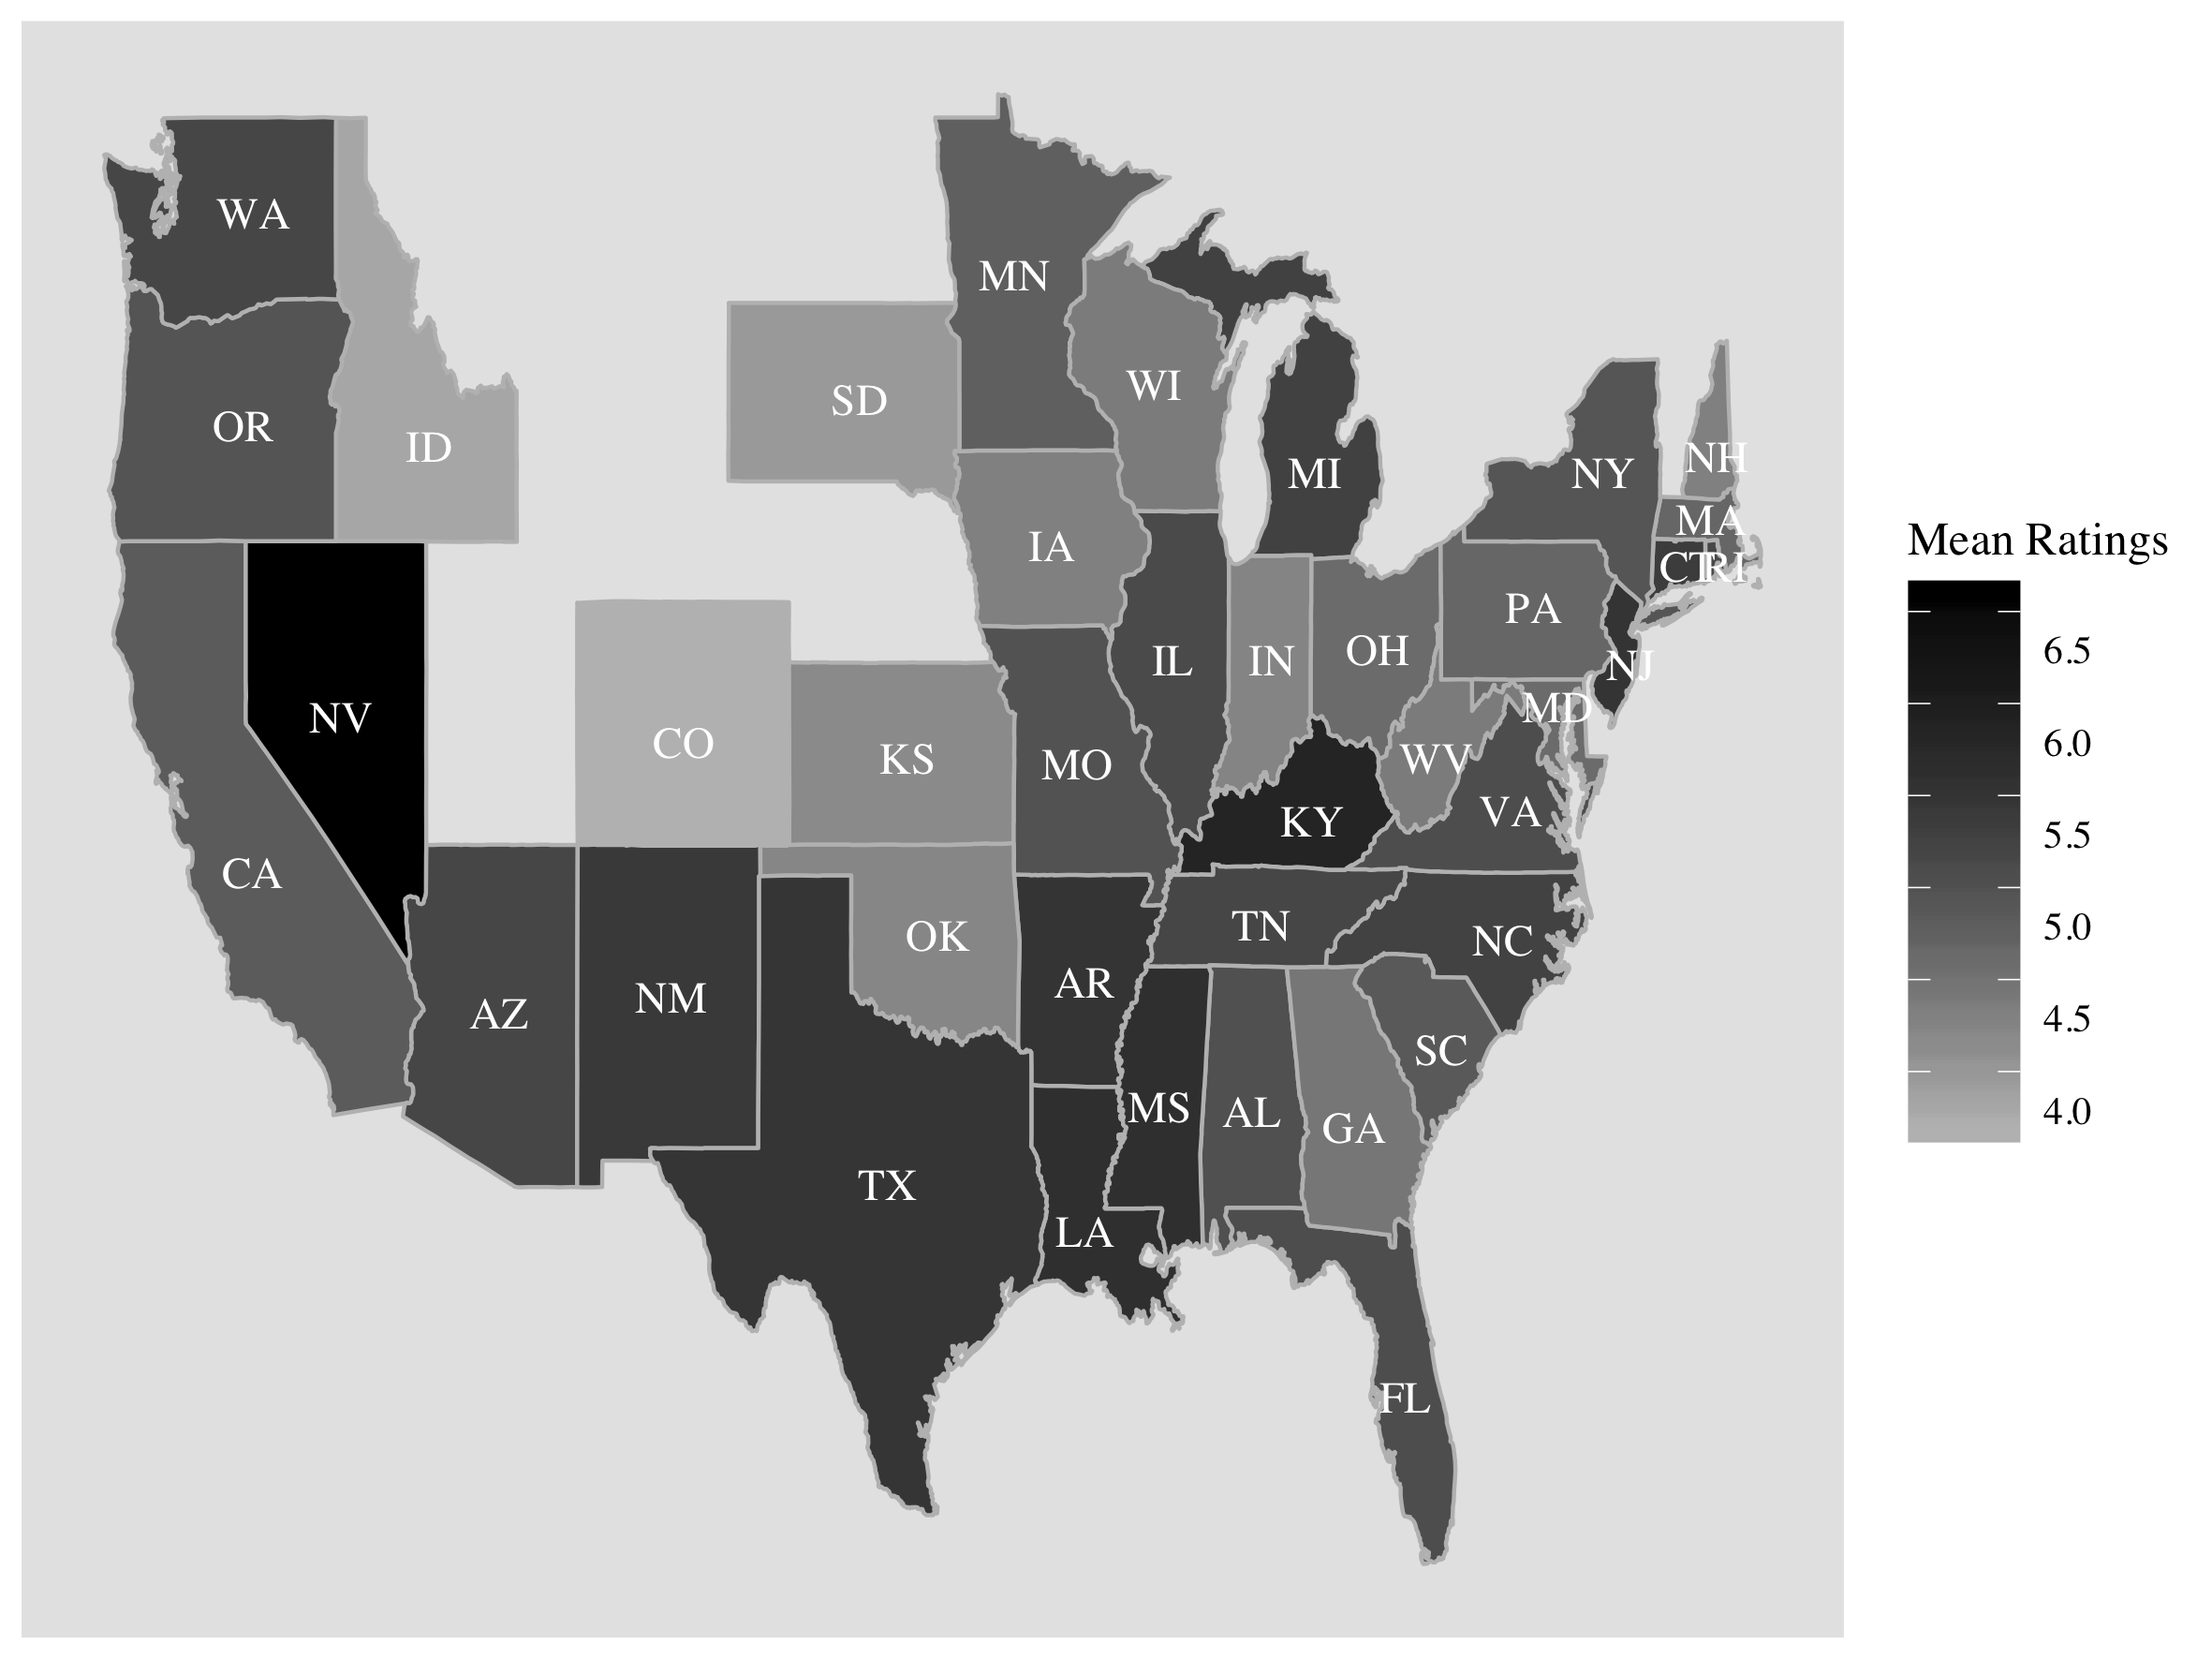
\includegraphics[width=0.8\textwidth]{figures/appendix/exp2.png}
    \caption{Mean Ratings by Birthplace (Experiment 2)}
    \label{fig:bp2}
  \figSpace
\end{figure}